% Options for packages loaded elsewhere
\PassOptionsToPackage{unicode}{hyperref}
\PassOptionsToPackage{hyphens}{url}
\PassOptionsToPackage{dvipsnames,svgnames,x11names}{xcolor}
%
\documentclass[
  letterpaper,
]{krantz}

\usepackage{amsmath,amssymb}
\usepackage{iftex}
\ifPDFTeX
  \usepackage[T1]{fontenc}
  \usepackage[utf8]{inputenc}
  \usepackage{textcomp} % provide euro and other symbols
\else % if luatex or xetex
  \usepackage{unicode-math}
  \defaultfontfeatures{Scale=MatchLowercase}
  \defaultfontfeatures[\rmfamily]{Ligatures=TeX,Scale=1}
\fi
\usepackage{lmodern}
\ifPDFTeX\else  
    % xetex/luatex font selection
\fi
% Use upquote if available, for straight quotes in verbatim environments
\IfFileExists{upquote.sty}{\usepackage{upquote}}{}
\IfFileExists{microtype.sty}{% use microtype if available
  \usepackage[]{microtype}
  \UseMicrotypeSet[protrusion]{basicmath} % disable protrusion for tt fonts
}{}
\makeatletter
\@ifundefined{KOMAClassName}{% if non-KOMA class
  \IfFileExists{parskip.sty}{%
    \usepackage{parskip}
  }{% else
    \setlength{\parindent}{0pt}
    \setlength{\parskip}{6pt plus 2pt minus 1pt}}
}{% if KOMA class
  \KOMAoptions{parskip=half}}
\makeatother
\usepackage{xcolor}
\usepackage{soul}
\setlength{\emergencystretch}{3em} % prevent overfull lines
\setcounter{secnumdepth}{5}
% Make \paragraph and \subparagraph free-standing
\ifx\paragraph\undefined\else
  \let\oldparagraph\paragraph
  \renewcommand{\paragraph}[1]{\oldparagraph{#1}\mbox{}}
\fi
\ifx\subparagraph\undefined\else
  \let\oldsubparagraph\subparagraph
  \renewcommand{\subparagraph}[1]{\oldsubparagraph{#1}\mbox{}}
\fi

\usepackage{color}
\usepackage{fancyvrb}
\newcommand{\VerbBar}{|}
\newcommand{\VERB}{\Verb[commandchars=\\\{\}]}
\DefineVerbatimEnvironment{Highlighting}{Verbatim}{commandchars=\\\{\}}
% Add ',fontsize=\small' for more characters per line
\usepackage{framed}
\definecolor{shadecolor}{RGB}{241,243,245}
\newenvironment{Shaded}{\begin{snugshade}}{\end{snugshade}}
\newcommand{\AlertTok}[1]{\textcolor[rgb]{0.68,0.00,0.00}{#1}}
\newcommand{\AnnotationTok}[1]{\textcolor[rgb]{0.37,0.37,0.37}{#1}}
\newcommand{\AttributeTok}[1]{\textcolor[rgb]{0.40,0.45,0.13}{#1}}
\newcommand{\BaseNTok}[1]{\textcolor[rgb]{0.68,0.00,0.00}{#1}}
\newcommand{\BuiltInTok}[1]{\textcolor[rgb]{0.00,0.23,0.31}{#1}}
\newcommand{\CharTok}[1]{\textcolor[rgb]{0.13,0.47,0.30}{#1}}
\newcommand{\CommentTok}[1]{\textcolor[rgb]{0.37,0.37,0.37}{#1}}
\newcommand{\CommentVarTok}[1]{\textcolor[rgb]{0.37,0.37,0.37}{\textit{#1}}}
\newcommand{\ConstantTok}[1]{\textcolor[rgb]{0.56,0.35,0.01}{#1}}
\newcommand{\ControlFlowTok}[1]{\textcolor[rgb]{0.00,0.23,0.31}{#1}}
\newcommand{\DataTypeTok}[1]{\textcolor[rgb]{0.68,0.00,0.00}{#1}}
\newcommand{\DecValTok}[1]{\textcolor[rgb]{0.68,0.00,0.00}{#1}}
\newcommand{\DocumentationTok}[1]{\textcolor[rgb]{0.37,0.37,0.37}{\textit{#1}}}
\newcommand{\ErrorTok}[1]{\textcolor[rgb]{0.68,0.00,0.00}{#1}}
\newcommand{\ExtensionTok}[1]{\textcolor[rgb]{0.00,0.23,0.31}{#1}}
\newcommand{\FloatTok}[1]{\textcolor[rgb]{0.68,0.00,0.00}{#1}}
\newcommand{\FunctionTok}[1]{\textcolor[rgb]{0.28,0.35,0.67}{#1}}
\newcommand{\ImportTok}[1]{\textcolor[rgb]{0.00,0.46,0.62}{#1}}
\newcommand{\InformationTok}[1]{\textcolor[rgb]{0.37,0.37,0.37}{#1}}
\newcommand{\KeywordTok}[1]{\textcolor[rgb]{0.00,0.23,0.31}{#1}}
\newcommand{\NormalTok}[1]{\textcolor[rgb]{0.00,0.23,0.31}{#1}}
\newcommand{\OperatorTok}[1]{\textcolor[rgb]{0.37,0.37,0.37}{#1}}
\newcommand{\OtherTok}[1]{\textcolor[rgb]{0.00,0.23,0.31}{#1}}
\newcommand{\PreprocessorTok}[1]{\textcolor[rgb]{0.68,0.00,0.00}{#1}}
\newcommand{\RegionMarkerTok}[1]{\textcolor[rgb]{0.00,0.23,0.31}{#1}}
\newcommand{\SpecialCharTok}[1]{\textcolor[rgb]{0.37,0.37,0.37}{#1}}
\newcommand{\SpecialStringTok}[1]{\textcolor[rgb]{0.13,0.47,0.30}{#1}}
\newcommand{\StringTok}[1]{\textcolor[rgb]{0.13,0.47,0.30}{#1}}
\newcommand{\VariableTok}[1]{\textcolor[rgb]{0.07,0.07,0.07}{#1}}
\newcommand{\VerbatimStringTok}[1]{\textcolor[rgb]{0.13,0.47,0.30}{#1}}
\newcommand{\WarningTok}[1]{\textcolor[rgb]{0.37,0.37,0.37}{\textit{#1}}}

\providecommand{\tightlist}{%
  \setlength{\itemsep}{0pt}\setlength{\parskip}{0pt}}\usepackage{longtable,booktabs,array}
\usepackage{calc} % for calculating minipage widths
% Correct order of tables after \paragraph or \subparagraph
\usepackage{etoolbox}
\makeatletter
\patchcmd\longtable{\par}{\if@noskipsec\mbox{}\fi\par}{}{}
\makeatother
% Allow footnotes in longtable head/foot
\IfFileExists{footnotehyper.sty}{\usepackage{footnotehyper}}{\usepackage{footnote}}
\makesavenoteenv{longtable}
\usepackage{graphicx}
\makeatletter
\def\maxwidth{\ifdim\Gin@nat@width>\linewidth\linewidth\else\Gin@nat@width\fi}
\def\maxheight{\ifdim\Gin@nat@height>\textheight\textheight\else\Gin@nat@height\fi}
\makeatother
% Scale images if necessary, so that they will not overflow the page
% margins by default, and it is still possible to overwrite the defaults
% using explicit options in \includegraphics[width, height, ...]{}
\setkeys{Gin}{width=\maxwidth,height=\maxheight,keepaspectratio}
% Set default figure placement to htbp
\makeatletter
\def\fps@figure{htbp}
\makeatother
\newlength{\cslhangindent}
\setlength{\cslhangindent}{1.5em}
\newlength{\csllabelwidth}
\setlength{\csllabelwidth}{3em}
\newlength{\cslentryspacingunit} % times entry-spacing
\setlength{\cslentryspacingunit}{\parskip}
\newenvironment{CSLReferences}[2] % #1 hanging-ident, #2 entry spacing
 {% don't indent paragraphs
  \setlength{\parindent}{0pt}
  % turn on hanging indent if param 1 is 1
  \ifodd #1
  \let\oldpar\par
  \def\par{\hangindent=\cslhangindent\oldpar}
  \fi
  % set entry spacing
  \setlength{\parskip}{#2\cslentryspacingunit}
 }%
 {}
\usepackage{calc}
\newcommand{\CSLBlock}[1]{#1\hfill\break}
\newcommand{\CSLLeftMargin}[1]{\parbox[t]{\csllabelwidth}{#1}}
\newcommand{\CSLRightInline}[1]{\parbox[t]{\linewidth - \csllabelwidth}{#1}\break}
\newcommand{\CSLIndent}[1]{\hspace{\cslhangindent}#1}

\usepackage{booktabs}
\usepackage{longtable}
\usepackage{array}
\usepackage{multirow}
\usepackage{wrapfig}
\usepackage{float}
\usepackage{colortbl}
\usepackage{pdflscape}
\usepackage{tabu}
\usepackage{threeparttable}
\usepackage{threeparttablex}
\usepackage[normalem]{ulem}
\usepackage{makecell}
\usepackage{xcolor}
\usepackage{amsmath}
\usepackage{caption}
\usepackage{fvextra}
\DefineVerbatimEnvironment{Highlighting}{Verbatim}{breaklines,commandchars=\\\{\}}
\makeatletter
\@ifpackageloaded{tcolorbox}{}{\usepackage[skins,breakable]{tcolorbox}}
\@ifpackageloaded{fontawesome5}{}{\usepackage{fontawesome5}}
\definecolor{quarto-callout-color}{HTML}{909090}
\definecolor{quarto-callout-note-color}{HTML}{0758E5}
\definecolor{quarto-callout-important-color}{HTML}{CC1914}
\definecolor{quarto-callout-warning-color}{HTML}{EB9113}
\definecolor{quarto-callout-tip-color}{HTML}{00A047}
\definecolor{quarto-callout-caution-color}{HTML}{FC5300}
\definecolor{quarto-callout-color-frame}{HTML}{acacac}
\definecolor{quarto-callout-note-color-frame}{HTML}{4582ec}
\definecolor{quarto-callout-important-color-frame}{HTML}{d9534f}
\definecolor{quarto-callout-warning-color-frame}{HTML}{f0ad4e}
\definecolor{quarto-callout-tip-color-frame}{HTML}{02b875}
\definecolor{quarto-callout-caution-color-frame}{HTML}{fd7e14}
\makeatother
\makeatletter
\makeatother
\makeatletter
\@ifpackageloaded{bookmark}{}{\usepackage{bookmark}}
\makeatother
\makeatletter
\@ifpackageloaded{caption}{}{\usepackage{caption}}
\AtBeginDocument{%
\ifdefined\contentsname
  \renewcommand*\contentsname{Table of contents}
\else
  \newcommand\contentsname{Table of contents}
\fi
\ifdefined\listfigurename
  \renewcommand*\listfigurename{List of Figures}
\else
  \newcommand\listfigurename{List of Figures}
\fi
\ifdefined\listtablename
  \renewcommand*\listtablename{List of Tables}
\else
  \newcommand\listtablename{List of Tables}
\fi
\ifdefined\figurename
  \renewcommand*\figurename{Figure}
\else
  \newcommand\figurename{Figure}
\fi
\ifdefined\tablename
  \renewcommand*\tablename{Table}
\else
  \newcommand\tablename{Table}
\fi
}
\@ifpackageloaded{float}{}{\usepackage{float}}
\floatstyle{ruled}
\@ifundefined{c@chapter}{\newfloat{codelisting}{h}{lop}}{\newfloat{codelisting}{h}{lop}[chapter]}
\floatname{codelisting}{Listing}
\newcommand*\listoflistings{\listof{codelisting}{List of Listings}}
\makeatother
\makeatletter
\@ifpackageloaded{caption}{}{\usepackage{caption}}
\@ifpackageloaded{subcaption}{}{\usepackage{subcaption}}
\makeatother
\makeatletter
\@ifpackageloaded{tcolorbox}{}{\usepackage[skins,breakable]{tcolorbox}}
\makeatother
\makeatletter
\@ifundefined{shadecolor}{\definecolor{shadecolor}{rgb}{.97, .97, .97}}
\makeatother
\makeatletter
\makeatother
\makeatletter
\makeatother
\ifLuaTeX
  \usepackage{selnolig}  % disable illegal ligatures
\fi
\IfFileExists{bookmark.sty}{\usepackage{bookmark}}{\usepackage{hyperref}}
\IfFileExists{xurl.sty}{\usepackage{xurl}}{} % add URL line breaks if available
\urlstyle{same} % disable monospaced font for URLs
\hypersetup{
  pdftitle={An Introduction to NFL Analytics with R},
  pdfauthor={Bradley J. Congelio},
  colorlinks=true,
  linkcolor={blue},
  filecolor={Maroon},
  citecolor={Blue},
  urlcolor={Blue},
  pdfcreator={LaTeX via pandoc}}

\title{An Introduction to NFL Analytics with R}
\author{Bradley J. Congelio}
\date{}

\begin{document}
\maketitle
\ifdefined\Shaded\renewenvironment{Shaded}{\begin{tcolorbox}[boxrule=0pt, interior hidden, breakable, borderline west={3pt}{0pt}{shadecolor}, enhanced, sharp corners, frame hidden]}{\end{tcolorbox}}\fi

\renewcommand*\contentsname{Table of contents}
{
\hypersetup{linkcolor=}
\setcounter{tocdepth}{2}
\tableofcontents
}
\bookmarksetup{startatroot}

\hypertarget{introduction}{%
\chapter{Introduction}\label{introduction}}

On April 27, 2020, Ben Baldwin hit send on a Tweet that announced the
birth of \texttt{nflfastR}, an R package designed to scrape NFL
play-by-play data, allowing the end-user to access it at speeds quicker
than similar predecessors (hence the name).

Thanks to the work of multiple people
(\href{https://twitter.com/mrcaseb}{@mrcaseB},
\href{https://twitter.com/benbbaldwin}{@benbbaldwin},
\href{https://twitter.com/_TanHo}{@TanHo},
\href{https://twitter.com/LeeSharpeNFL}{@LeeSharpeNFL}, and
\href{https://twitter.com/thomas_mock}{@thomas\_mock} \ldots{} to just
name a few), the process of getting started with advanced analytics
using NFL data is now easier than ever.

That said, and without getting too far into the weeds of the history
behind it all, the above-mentioned people are responsible in some shape
or form for the current status of the \texttt{nflverse}, which is a
superb collection of data and R-based packages that allows anybody the
ability to access deeply robust NFL data as far back as the 1999 season.

The \texttt{nflverse} as we know it today was initially birthed from the
\texttt{nflscrapR} project, which was started by the Carnegie Mellon
University student and profess duo of
\href{https://twitter.com/bklynmaks?lang=en}{Maksim Horowitz} and
\href{https://twitter.com/stat_sam}{Sam Ventura}. After Horowitz
graduated - and got hired by the Atlanta Hawks - the \texttt{nflscrapR}
package was taken over by fellow CMU student Ron Yurko (who would go on
to receive his Ph.D.~from the Statistics and Data Science program). The
trio's work on \texttt{nflscrapR} ultimately led to a peer-reviewed
paper titled ``\href{https://arxiv.org/pdf/1802.00998.pdf}{nflWAR: A
Reproducible Method for Offensive Player Evaluation in Football.}''
Ultimately, the \texttt{nflscrapR} project came to an end when the
specific .json feed used to gather NFL data changed. At this point, Ben
Baldwin and Sebastian Carl had already built upon the \texttt{nflscrapR}
project's foundations to create \texttt{nflfastR}. Ron officially marked
the end of the \texttt{nflscrapR} era and the beginning of the
\texttt{nflfastR} era with a tweet on September 14, 2020:\footnote{Thanks
  to Ben Baldwin for chatting with me on Discord and providing this
  brief understanding of the backstory.}

As a reply to his first tweet about the \texttt{nflfastR} project, Ben
explained that he created the original function to scrape NFL data for
the creation of his \href{https://rbsdm.com/stats/stats/}{NFL analytics
website}. Thankfully, he and Seb did not keep the creation to themselves
and released \texttt{nflfastR} to the public. Because of the ``open
source'' nature of R and R packages, a laundry list of companion
packages quickly developed alongside \texttt{nflfastR}. The original
\texttt{nflfastR} package is now part of the larger \texttt{nflverse} of
packages that drive the NFL analytics community on Twitter and beyond.

The creation of the \texttt{nflverse} allowed for anybody interested in
NFL analytics to easily access data, manipulate it to their liking, and
release their visualizations and/or metrics to the wider public. In
fact, it is now a regular occurrence for somebody to advance their R
programming ability because of the \texttt{nflverse} and then go on to
win the Big Data Bowl. As of the 2022 version of the Big Data Bowl, over
``30 participants have been hired to work in data and analytics roles in
sports, including 22 that were hired in football'' ({``Big Data Bowl:
The Annual Analytics Contest Explores Statistical Innovations in
Football,''} n.d.). Most recently, the
\href{https://www.boltsfromtheblue.com/2021/7/9/22570490/chargers-news-nfl-big-data-bowl}{Chargers
hired 2020 participate Alex Stern} and the
\href{https://twitter.com/sethwalder/status/1532721476209627136}{Chiefs
hired Marc Richards}, a member of the winning 2021 team, as a Football
Research Analyst.

Kevin Clark, in a 2018 article for
\href{https://www.theringer.com/nfl/2018/12/19/18148153/nfl-analytics-revolution}{\emph{The
Ringer}}, explained that despite not being as obvious as the
sabermetrics movement in baseball, the analytics movement in the NFL is
``happening in front of you all the time.'' The use of analytics in the
NFL did, however, predate Clark's article. In 2014, Eagles head coach
Doug Pederson explained that all decisions made by the organization -
from game planning to draft strategy - were to be informed by hard data
and analytics. Leading this early adoption of analytics, and reporting
directly to team Vice President Howie Roseman, were Joe Douglas and Alec
Halaby, ``a 31-year-old Harvard grad with a job description'' that had
an emphasis on ``integrating traditional and analytical methods in
football decision-making.'' The result? A ``blending of old-school
scouting and newer approaches'' that were often only seen in other
leagues, such as the NBA and MLB (Rosenthal 2018). Pederson believed in
and trusted the team's approach to analytics so much that a direct line
of communication was created between the two during games, with the
analytics department providing the head coach with math-based
recommendations for any scenario Pederson requested (Awbrey
2020).\footnote{Thanks, again, to Ben Baldwin for providing his personal
  knowledge about the ``early days'' of the Eagles' analytics
  department.}

In just under five years time since the publishing of that article, it
has become hard to ignore the analytic movement within the NFL. Yet,
there is still so much growth to happen in the marriage between the NFL
and advanced metrics. For example, there is no denying that the
sabermetrics movement drastically ``altered baseball's DNA'' Heifetz
(2019){]}. Moreover, as explained in Seth Partnow's outstanding
\href{https://www.amazon.com/Midrange-Theory-Basketballs-Evolution-Analytics/dp/1637270968/ref=tmm_pap_swatch_0?_encoding=UTF8\&qid=1656245879\&sr=8-4}{\emph{The
Midrange Theory: Basketball's Evolution in the Age of Analytics}}, the
analytics movement in the NBA essentially killed the midrange shot
(briefly: it is more beneficial to try to work the ball in directly
under the basket (for a high-percentage shot) or to take the 3-pointer,
as the possible additional point is statistically worth more despite the
lower success probability as opposed a 2-point midrange shot) as well as
the traditional, ``old-school'' center position.

Compared to both the NBA and MLB, the NFL is playing catch up in
analytics driving changes equivalent to the death of the midrange shot
or the plethora of additional tactics and changes to baseball because of
sabermetrics. Joe Banner, who served as the President of the Eagles from
2001-2012 and then the Chief Executive Officer of the Browns from
2012-2013, explained that some of the hesitation to incorporate
analytics into NFL game planning was a result of the game being ``very
much driven by conventional wisdom to an extreme degree'' (Fortier
2020). Perhaps nobody encapsulates this better than Pittsburgh Steelers
Head Coach Mike Tomlin. When asked about his position on analytics
during the 2015 season, Tomlin explained:

\begin{quote}
I think that's why you play the game. You can take analytics to baseball
and things like that but football is always going to be football. I got
a lot of respect for analytics and numbers, but I'm not going to make
judgements based on those numbers. The game is the game. It's an
emotional one played by emotional and driven men. That's an element of
the game you can't measure. Often times decisions such as that weigh
heavily into the equation (Kozora 2015).
\end{quote}

Given that Tomlin's quote is from 2015, perhaps the Steelers pivoted
since and are now more analytically inclined. That does not seem to be
the case. In a poll of NFL analytics staffers conducted by ESPN,
\href{https://www.espn.com/nfl/story/_/id/29939438/2020-nfl-analytics-survey-which-teams-most-least-analytically-inclined\#least}{the
Steelers were voted as one of the least analytically advanced teams in
the league.}

There is large gap between the least analytically inclined teams
(Washington, Tennessee, Cincinnati, New York Giants, and Pittsburgh) and
those voted as the most analytically inclined (Baltimore, Cleveland,
Philadelphia, and Houston). In the ESPN poll, the Browns were voted as
the analytics department producing the highest level of work. One of
those polled spoke to the fact that much of this outstanding work is a
result of General Manager Andrew Berry being a ``true believer,''
explaining that he is one of the ``rare guys you'll come across in life
where you think to yourself, `Man, this guy thinks at a different level.
Just pure genius.' He's one of them.''

\href{https://www.washingtonpost.com/sports/2020/01/16/nfls-analytics-movement-has-finally-reached-sports-mainstream/}{In
his article for the \emph{Washington Post}}, Sam Fortier argues that
many teams became inspired to more intimately introduce analytics into
game planning and on-field decisions after the 2017 season. On their run
to becoming Super Bowl Champions, the Philadelphia Eagles were
aggressive on 4th down, going for it 26 times during the season and
converting on 17 of those for a conversion percentage of 65.4\%. A quick
examination and visualization of data highlights the absolutely
staggering increase in 4th aggressiveness among NFL head coaches from
2017-2021:

\begin{figure}

{\centering 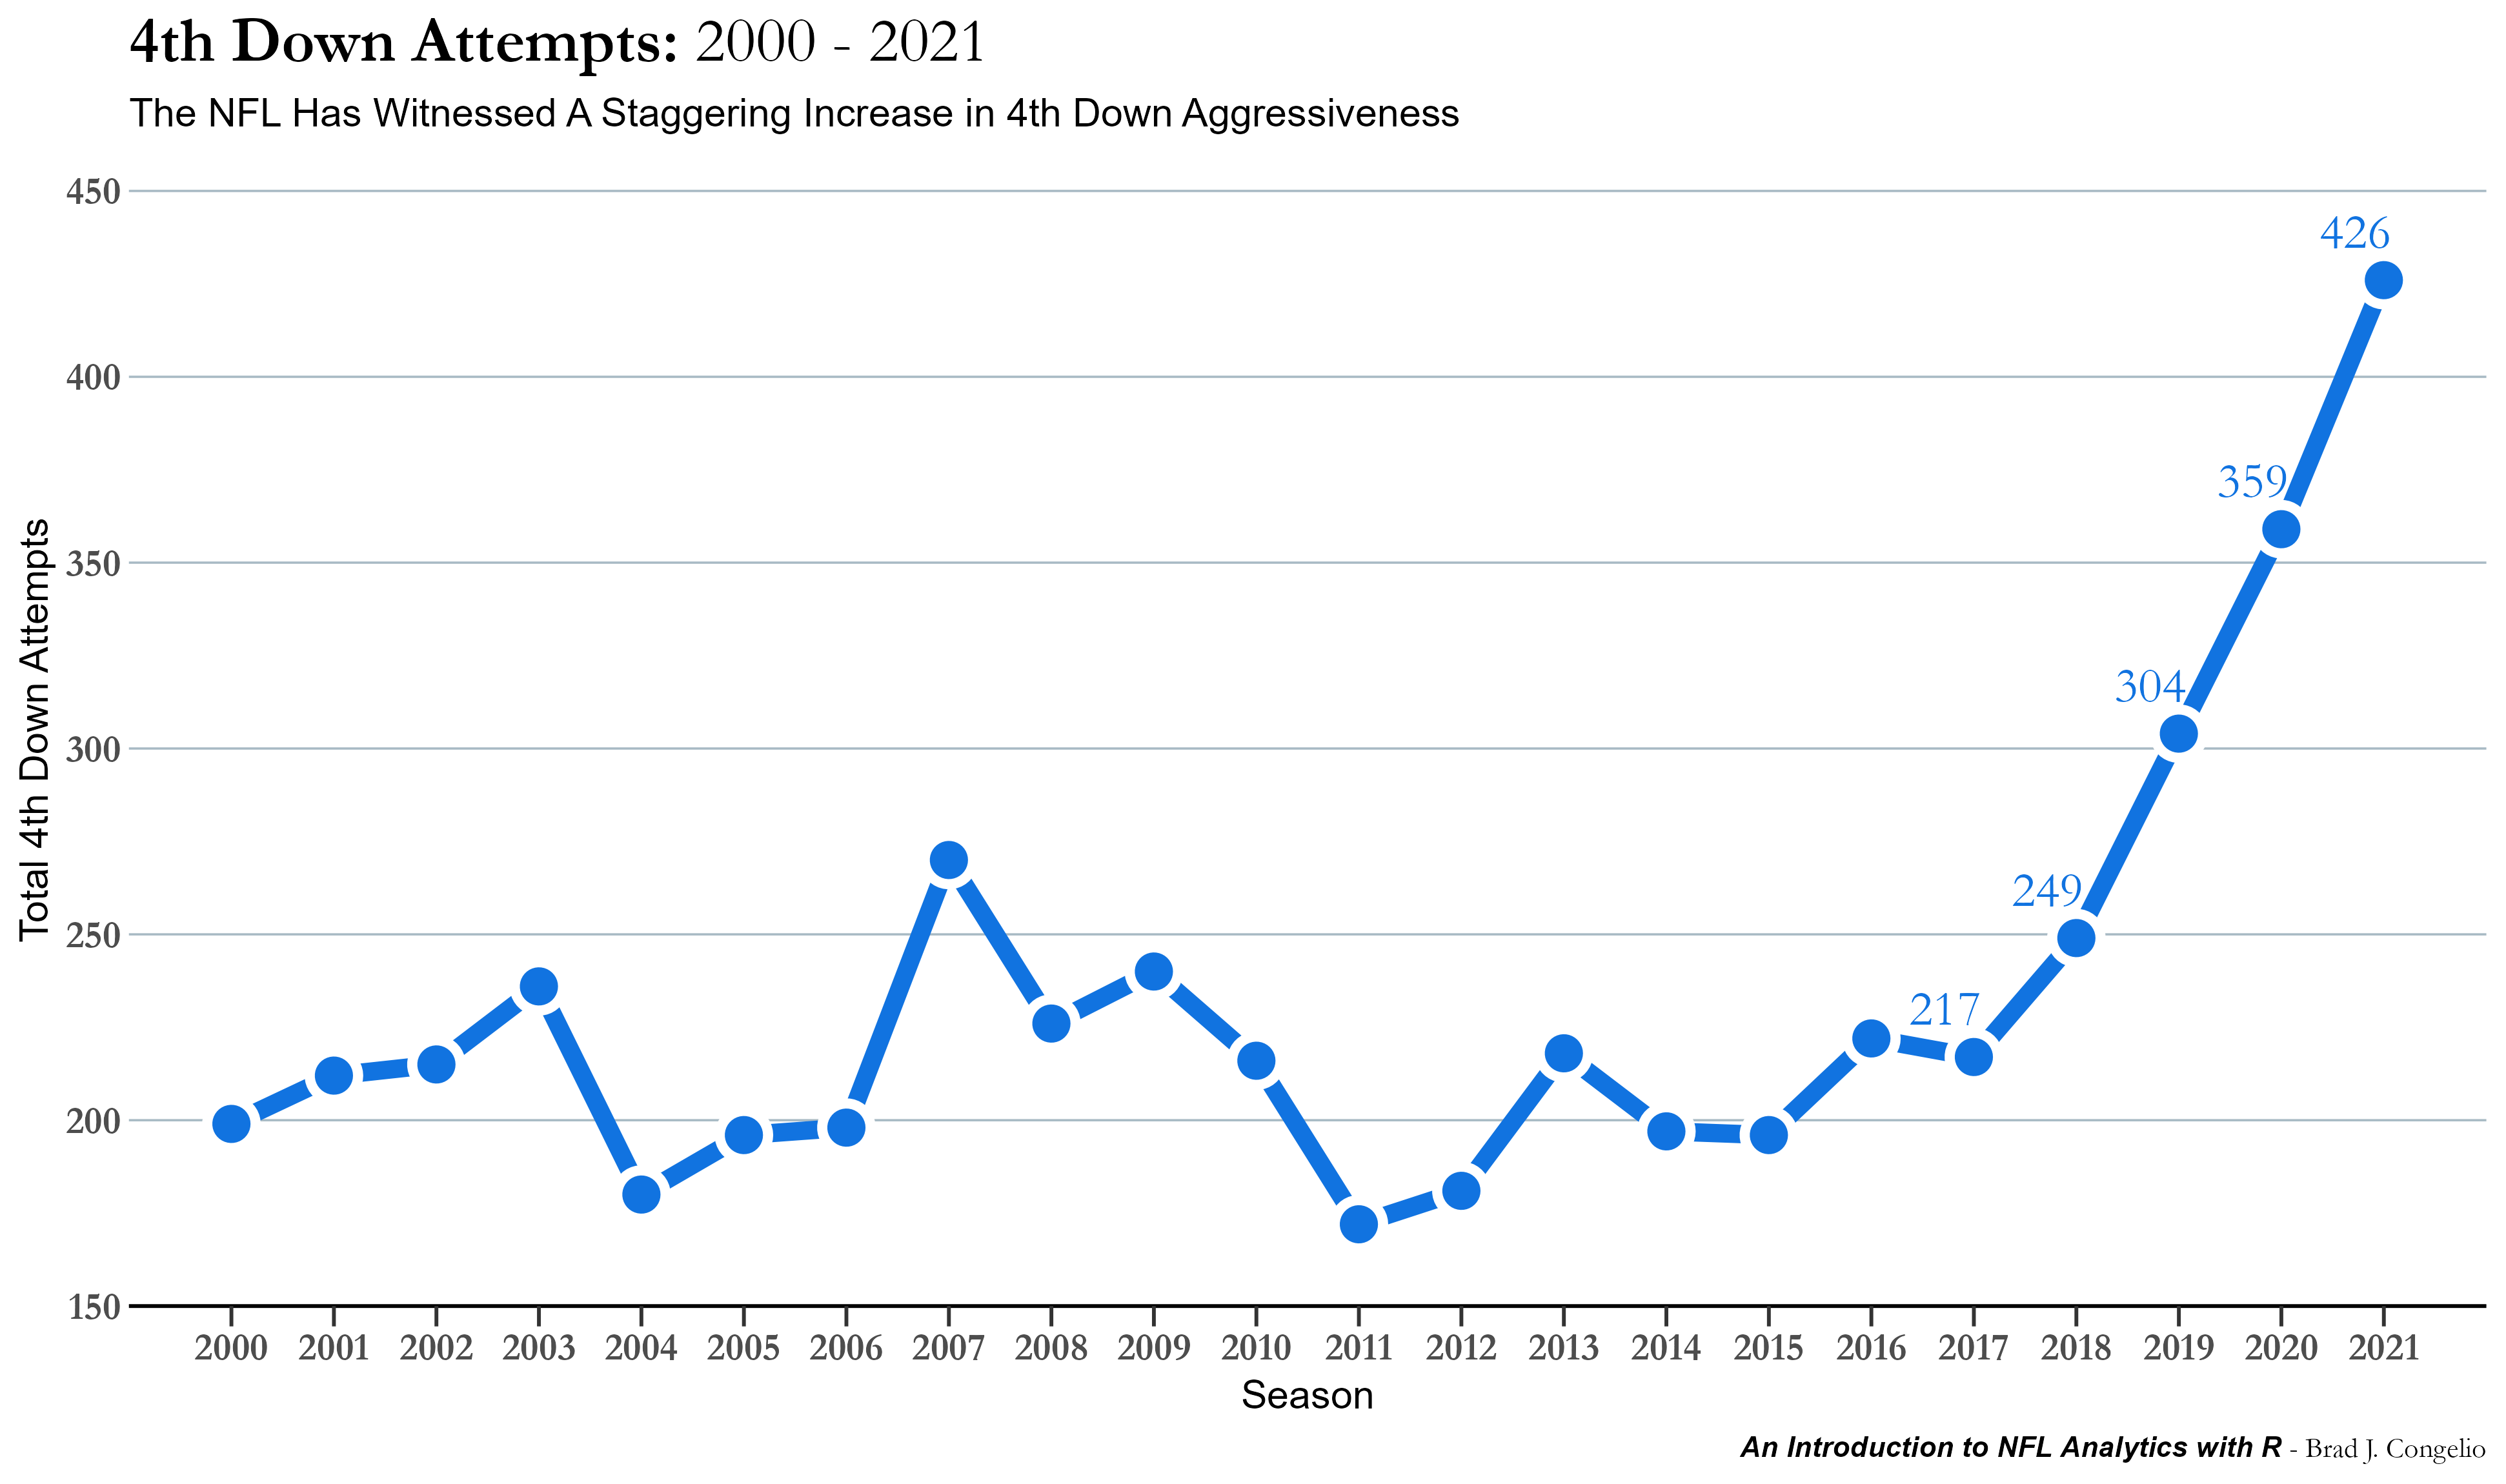
\includegraphics[width=9.71in,height=\textheight]{images/4th-down-attempts.png}

}

\caption{4th Down Attempts: 2000 - 2021}

\end{figure}

There has been a 96.3\% increase in the number of 4th down attempts from
just 2017 to 2021. In fact, the numbers may actually be higher as I was
quite conservative in building the above plot by only considering those
4th down attempts that took place when the offensive team had between a
5-to-95\% winning probability and those prior to the two-minute warning
of either half. Even with those conservative limitations, the increase
is staggering. The numbers, however, support this aggression. During
week one of both the 2020 and 2021 season, \emph{not} going for it on
4th down ``cost teams a cumulative 170 percentage points of win
probability'' (Bushnell 2021).

Ben Baldwin, using the \texttt{nfl4th} package that is part of the
\texttt{nflverse}, tracked the shift in NFL coaching mentality regarding
4th down decisions by comparing 2014's ``go for it percentage'' against
the same for 2020. When compared to the 2014 season, NFL coaches are now
much more in agreement with analytics on when to ``go for it'' on 4th
down in relation to the expected gain in win probability.

\begin{figure}

{\centering \includegraphics[width=36in,height=\textheight]{images/baldwin-graph-goforit.png}

}

\caption{Credit: Ben Baldwin}

\end{figure}

It should not be surprising then, considering Mike Tomlin's quote from
above and other NFL analytics staffers voting the Steelers as one of the
least analytically driven teams in the league, that Pittsburgh lost the
most win probability by either kicking or punting in ``go for it''
situations during the 2020 NFL season. On the other end, the Ravens and
Browns - two teams voted as the most analytically inclined - are the two
best organizations at knowing when to ``go for it'' on 4th down based on
win probability added. There seems to be a defined relationship between
teams buying into analytics and those who do not:

\begin{figure}

{\centering \includegraphics[width=36in,height=\textheight]{images/tomlin-go-for-it.png}

}

\caption{Credit: Ben Baldwin}

\end{figure}

The NFL's turn towards more aggressive 4th-down decisions is just one of
the many analytics-driven changes occurring in the league. Another
significant example is Defense-Adjusted Value over Average (or DVOA), a
formula created by Aaron Schatz, now the editor in chief of
\href{https://www.footballoutsiders.com/info/methods\#dvoa}{Football
Outsiders}, that sought to challenge the notion that teams should,
first, establish the running game in order to open up the passing game.
Some of these changes are apparent on televisions screens on Sunday
afternoons in the Fall, while others are occurring behind the scenes
(analytics departments working on scouting and draft preparation, for
example). Indeed, the use of analytics in the NFL is not as tightly
ingrained as we see in other prominent leagues. And we must remember
that there are certainly continued hold outs among some NFL coaches
(like Mike Tomlin).

Despite some coaching hold outs on fully embracing analytics, the
``thirst for knowledge in football is as excessive as any other sport
and the desire to get the most wins per dollar is just as high.'' As the
pipeline of data continues to grow, both internally in the league and
data that becomes publicly accessible, ``smart teams will continue to
leave no rock unturned as they push the limits on how far data can take
them.'' Joe Banner explained that while the NFL has long been a league
of coaches saying ``well, that is the way we've always done it,'' the
league is ripe for a major shift (Bechtold 2021).

Banner's belief that those teams searching for every competitive
advantage will ``leave no rock unturned'' is the driving force behind
this book. For all intents and purposes, the age of analytics in the NFL
is still in its infancy. Turning back, again, to the 2017 season, the
Eagles' management praised and credited the team's analytics department
as part of the reason they were able to win Super Bowl LII. Doing so
Danney Heifetz argues, ``changed the language of football.'' The NFL, he
explains, is a ``copycat league'' and, as witnessed with the increase in
4th down aggressiveness since 2017, teams immediately began to carbon
copy Philadelphia's approach to folding traditional football strategy
with a new age analytics approach. Because of the modernity of this
relationship between long-held football dogmas and analytics, nobody can
be quite sure what other impacts it will create on the gamesmanship of
football.

However, as Heifetz opines, both the NBA and MLB can serve as a roadmap
to where analytics will take the NFL. Importantly, the NFL's
relationship with analytics is still in its ``first frontier of what
will likely be a sweeping change over the next two decades.'' Because of
this, we cannot be sure what the next major impact analytics will make,
nor when it may occur. But, with the ever-growing amount of publicly
accessible data, it is only a matter of time until it is discovered. For
example, in an interview with Heifetz, Brian Burke - one of the
forefather's of NFL analytics and now a writer for ESPN - expressed his
belief that the next major impact will be ``quantifying how often
quarterbacks make the correct decision on the field.''

It seems that every new NFL season results in an amateur analyst
bringing a groundbreaking model and/or approach to the table. Unlike,
for example, MLB where there is little left to discover in terms of
sabermetrics and new approaches to understanding the game and its
associated strategy, the NFL is - for lack of a better phrase - an open
playing field. With more and more data becoming available to the public,
it is now easier than ever investigate your own ideas and suspicions and
to create your own models to confirm your intuition.

For example, I am originally from the greater Pittsburgh area and am a
big Steelers fan (which certainly explains some of the Steelers-centric
examples I use in the writing of this book). I was adamant in my belief
that Pittsburgh's TJ Watt should win the 2021 Defensive Player of the
Year award, despite many others calling for Los Angeles' Aaron Donald to
claim the title. In effort to prove my point, I sought out to design
what I coined \textbf{\emph{Adjusted Defensive Impact}}. To begin, I
wanted to explore the idea that not all defensive sacks are created
equal, as a player's true impact is not always perfectly represented by
top-level statistics.

To account for that, I opted to adjust and add statistical weight to
sack statistics. This was done over multiple areas. For instance, not
all players competed in all 17 regular-season games in 2021. To adjust
for this, I took the total of game played in the data (2,936) and
divided by 17 (a full season) to achieve a weighted adjustment of
0.0058. TJ Watt played in just 15 games in 2021. His adjusted equation,
therefore, is (17-`games') * 0.0058. The result? He gets a bit more
credit for this adjustment than, say, Myles Garrett who played all 17
regular-season games.

Going further with the model, I created a weighted adjustment for solo
sacks (0.90), a negative weighted adjustment (-0.14) for any sack
charted as ``unblocked,'' and a weighted adjustment to account for how
many times a player actually rushed the QB compared to how many
defensive snaps they played. Using data from the SIS Data Hub, the full
code is below:

\begin{Shaded}
\begin{Highlighting}[]
\FunctionTok{options}\NormalTok{(}\AttributeTok{digits =} \DecValTok{2}\NormalTok{)}

\NormalTok{pass.data }\OtherTok{\textless{}{-}}\NormalTok{ pass\_rush\_data }\SpecialCharTok{\%\textgreater{}\%}
  \FunctionTok{select}\NormalTok{(Player, Team, Games, }\StringTok{\textasciigrave{}}\AttributeTok{Pass Snaps}\StringTok{\textasciigrave{}}\NormalTok{, }\StringTok{\textasciigrave{}}\AttributeTok{Pass Rushes}\StringTok{\textasciigrave{}}\NormalTok{,}
         \StringTok{\textasciigrave{}}\AttributeTok{Solo Sacks}\StringTok{\textasciigrave{}}\NormalTok{, }\StringTok{\textasciigrave{}}\AttributeTok{Ast. Sacks}\StringTok{\textasciigrave{}}\NormalTok{, }\StringTok{\textasciigrave{}}\AttributeTok{Comb. Sacks}\StringTok{\textasciigrave{}}\NormalTok{, }
         \StringTok{\textasciigrave{}}\AttributeTok{Unblocked Sacks}\StringTok{\textasciigrave{}}\NormalTok{, Hurries, Hits) }\SpecialCharTok{\%\textgreater{}\%}
  \FunctionTok{rename}\NormalTok{(}\AttributeTok{total.snaps =} \StringTok{\textasciigrave{}}\AttributeTok{Pass Snaps}\StringTok{\textasciigrave{}}\NormalTok{,}
         \AttributeTok{total.rushes =} \StringTok{\textasciigrave{}}\AttributeTok{Pass Rushes}\StringTok{\textasciigrave{}}\NormalTok{,}
         \AttributeTok{solo.sacks =} \StringTok{\textasciigrave{}}\AttributeTok{Solo Sacks}\StringTok{\textasciigrave{}}\NormalTok{,}
         \AttributeTok{asst.sacks =} \StringTok{\textasciigrave{}}\AttributeTok{Ast. Sacks}\StringTok{\textasciigrave{}}\NormalTok{,}
         \AttributeTok{comb.sacks =} \StringTok{\textasciigrave{}}\AttributeTok{Comb. Sacks}\StringTok{\textasciigrave{}}\NormalTok{,}
         \AttributeTok{unblocked.sacks =} \StringTok{\textasciigrave{}}\AttributeTok{Unblocked Sacks}\StringTok{\textasciigrave{}}\NormalTok{,}
         \AttributeTok{player =}\NormalTok{ Player,}
         \AttributeTok{team =}\NormalTok{ Team,}
         \AttributeTok{games =}\NormalTok{ Games,}
         \AttributeTok{hurries =}\NormalTok{ Hurries,}
         \AttributeTok{hits =}\NormalTok{ Hits)}

\NormalTok{pass.data}\SpecialCharTok{$}\NormalTok{rush.percent }\OtherTok{\textless{}{-}}\NormalTok{ pass.data}\SpecialCharTok{$}\NormalTok{total.rushes }\SpecialCharTok{/}\NormalTok{ pass.data}\SpecialCharTok{$}\NormalTok{total.snaps}

\NormalTok{calculated.impact }\OtherTok{\textless{}{-}}\NormalTok{ pass.data }\SpecialCharTok{\%\textgreater{}\%}
  \FunctionTok{group\_by}\NormalTok{(player) }\SpecialCharTok{\%\textgreater{}\%}
  \FunctionTok{summarize}\NormalTok{(}
    \AttributeTok{adjusted.games =}\NormalTok{ (}\DecValTok{17} \SpecialCharTok{{-}}\NormalTok{ games) }\SpecialCharTok{*} \FloatTok{0.0058}\NormalTok{,}
    \AttributeTok{adjusted.solo =}\NormalTok{ solo.sacks }\SpecialCharTok{*} \FloatTok{0.9}\NormalTok{,}
    \AttributeTok{adjusted.unblocked =}\NormalTok{ unblocked.sacks }\SpecialCharTok{/} \SpecialCharTok{{-}}\FloatTok{0.14}\NormalTok{,}
    \AttributeTok{adjusted.rush.percent =} \FloatTok{0.81} \SpecialCharTok{{-}}\NormalTok{ rush.percent,}
    \AttributeTok{combined.impact =} \FunctionTok{sum}\NormalTok{(adjusted.games }\SpecialCharTok{+} 
\NormalTok{                            (solo.sacks }\SpecialCharTok{*} \FloatTok{0.9}\NormalTok{) }\SpecialCharTok{+} 
\NormalTok{                            (unblocked.sacks }\SpecialCharTok{*} \SpecialCharTok{{-}}\FloatTok{0.14}\NormalTok{) }\SpecialCharTok{+} 
\NormalTok{                            adjusted.rush.percent))}
\end{Highlighting}
\end{Shaded}

The end result? Taking into account the above adjusted defensive impact,
TJ Watt was absolutely dominant during the 2021 season:

\begin{figure}

{\centering 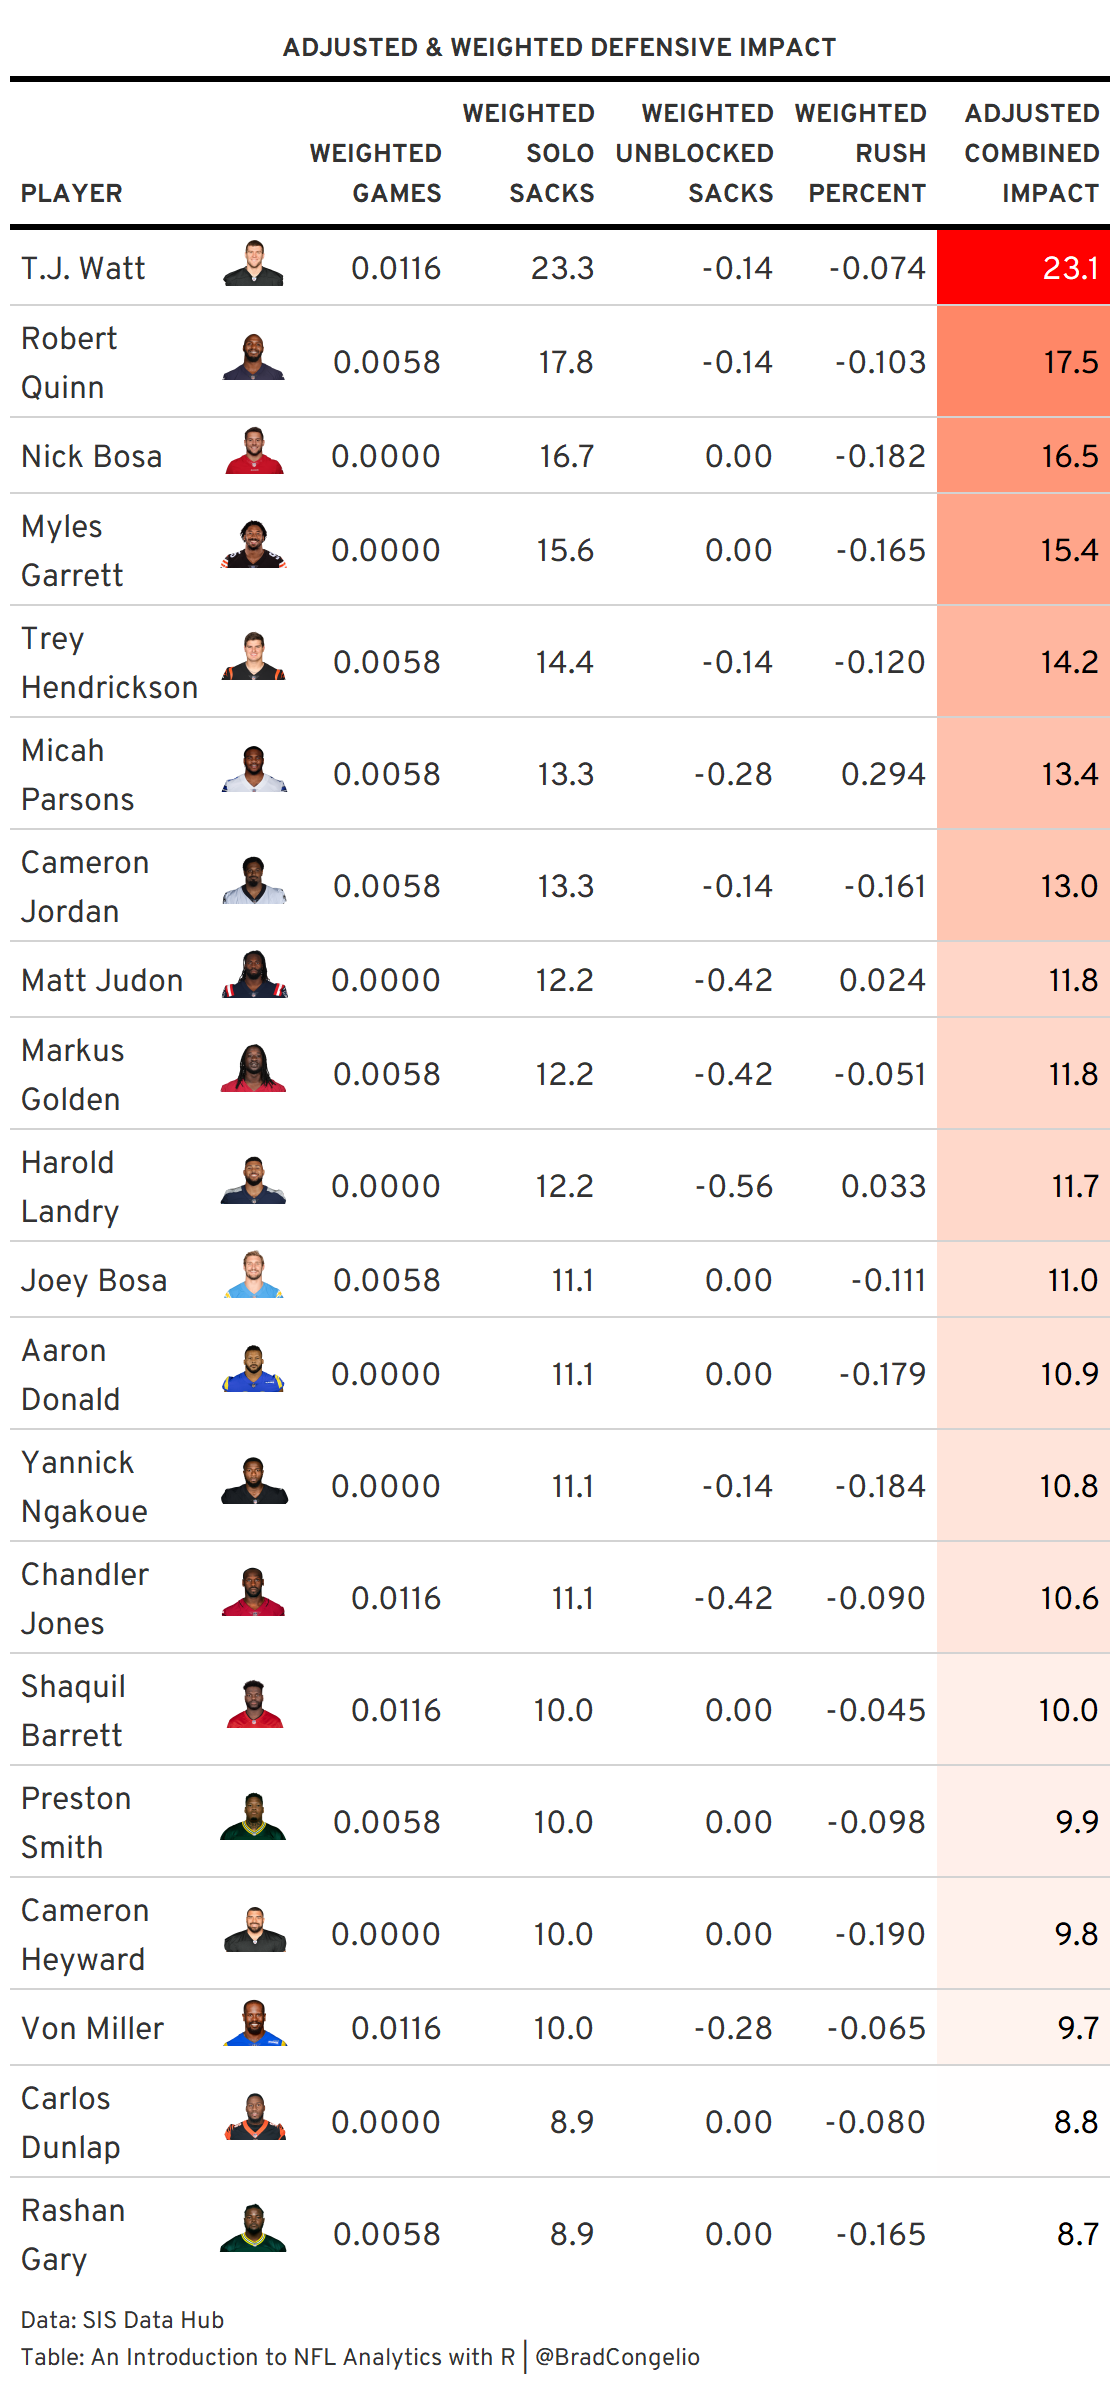
\includegraphics[width=2.8in,height=\textheight]{images/adjusteddefense.png}

}

\caption{Adjusted Defensive Impact}

\end{figure}

All of these examples - from Ben Baldwin's 4th-down model, to Football
Outsiders' DVOA, to my attempt to further quantify defensive player
impact - are just the leading edge of the burgeoning analytics movement
in the NFL. Moreover, the beauty of analytics is that you do not have to
be a mathematician or statistics buff in order to enter the fray. All it
takes is a genuine curiosity to explore what Bob Carroll, Pete Palmer,
and John Thorn coined as the ``\href{https://amzn.to/3y1GZTO}{Hidden
Game of Football}'' and the desire to learn, if you have not already,
the R programming language.

\hypertarget{who-this-book-is-for}{%
\subsection{Who This Book Is For}\label{who-this-book-is-for}}

Writing a book that is wholly dependent on the R programming language to
achieve the end goals is not an easy task, as there are likely two types
of people reading this: those with familiarity in R and those without.
If you are part of the former group, you can likely skip chapter 2 as it
is a primer on installing R and learning the language of the
\texttt{tidyverse}. On the other hand, if you are part of the latter
group, you should skip ahead to chapter 2 before even looking at chapter
1, which serves as an introduction to the \texttt{nflverse} with
examples. That said, this book can serve multiple audiences:

\begin{enumerate}
\def\labelenumi{\arabic{enumi}.}
\item
  Those interested in learning how to produce NFL analytics regardless
  of their current knowledge of the R programming language.
\item
  Professors who instruct data science courses can provide lessons
  through the lens of sport or, perhaps better, create their own Sport
  Analytics courses designed around the book. Moreover, future plans for
  this book include instruction reference guides to include PowerPoint
  templates, assignments/project instructions and grading rubrics, and
  quiz/exam content for online management systems (D2L, Canvas, Moodle,
  etc.).
\item
  Students are able to use this book in multiple ways. For example, in
  my Sport Analytics course, students are first introduced to R and the
  \texttt{tidyverse} using the built-in R data sets (\texttt{mtcars},
  \texttt{iris}, and \texttt{nycflights13}). While those data sets
  certainly serve a purpose, I have found that students grasp the
  concepts and language of the \texttt{tidyverse} more quickly when the
  class turns to using data from the \texttt{nflverse}. Because of this,
  students can use this book to start learning the R programming
  language using football terms (passing yards, first downs, air yards,
  completion percentage over expected) as opposed to the variables they
  may find much less interesting housed in the built-in data. Moreover,
  students already fluid in R can use this book to construct machine
  learning models using football data, for example, as part of
  assignments in data science/analytics courses.
\item
  Journalists, bloggers, and arm-chair quarterbacks alike can use the
  book to underpin their arguments and to provide hard data to backup
  their claims.
\end{enumerate}

It is also important to note that it is not expected for you to be an
expert in statistics, coding, or data modeling in order to find this
book useful. In fact, I self-taught myself the R programming language
after discovering its potential usefulness in my personal academic
research. I only ``became more serious'' about advancing my
understanding of the language's nuances, and more advanced methods,
after discovering the \texttt{nflscrapR} package and using it as my
learning tool for the deep dive into R. My decision to pursue an
academic certificate in the language was driven by the creation of my
Sport Analytics course, as the certificate provided the ``academic
training'' proof that was necessary to move the course through the
University's curriculum committee. Nonetheless, because of this
self-taught journey - and despite being an academic myself - I find that
I largely avoid the use of ``complicated jargon'' that is so evident in
most formal writing.

Because of this, and regardless of which chapter you begin with, I
believe that this book achieves its main goal: to provide a gentle
introduction to doing NFL analytics with R.

As this book is published online, it allows me to continue real-time
development of it. Because of this, make note of the following:

\begin{itemize}
\item
  \emph{Introduction to NFL Analytics with R} is published through CRC
  Press.
\item
  Please feel free to contribute to the book by filing an issue or
  making a pull request at the book's GitHub repository:
  \href{https://github.com/bcongelio/nfl-analytics-with-r-book}{\emph{Introduction
  to NFL Analytics with R} Github Repository}
\item
  The majority of the chapters conclude with exercises. In some cases,
  prepared data will be provided with a link to download the file. In
  other cases, you are expected to use the \texttt{nflverse} to collect
  the data yourself. In either case, the book's github repository for
  the exercises (link to the specific directory coming soon) will
  include the R files that contain the answers to each exercise.
\item
  Soon there will be a YouTube series to go along with the written
  version of this book. In brief, the videos will include my going over
  each chapter, step-by-step, with additional instruction and/or
  approaches.
\item
  Are you an instructor hoping to create or grow your Sport Analytics
  course? Future plans for this book include the creation of Instructor
  Materials to include an example syllabus plus structured lesson plans,
  exercises, assignments, quizzes, and exams. As well, templates for
  lectures will be included in PowerPoint form so you may edit to fit
  your specific needs.
\end{itemize}

\hypertarget{overview-of-chapters}{%
\section{Overview of Chapters}\label{overview-of-chapters}}

\begin{itemize}
\item
  \textbf{Chapter 1} provides an overview of the \texttt{nflverse} with
  specific attention paid to the difference between using
  \texttt{nflfastR} versus \texttt{nflreadr}. Serving as the first dive
  into analytics, the chapter showcases how to use \texttt{nflreadr} to
  retrieve both compiled weekly NFL stats and the deeply robust
  play-by-play statistics. In both cases, exercises are provided.
  Readers will do their first coding by, first, using the weekly stats
  to determine the 2021 leaders in air yards per attempt. Second,
  readers will use the play-by-play statistics from the 2021 season to
  create a brand new metric (QB aggressiveness on 3rd down pass
  attempts). Afterward, readers will learn how to retrieve multiple
  seasons of data at once.
\item
  \textbf{Chapter 2} covers the process of downloading both R and
  RStudio, as well as the necessary packages to do NFL analytics. As one
  of the most important chapters in the book (especially for those new
  to the R programming language), readers take a deep dive into
  wrangling NFL data with the \texttt{tidyverse} package. To begin,
  readers will learn about the \texttt{dplyr} pipe
  (\texttt{\%\textgreater{}\%}) and use, in exercises, the six most
  important verbs in the \texttt{dplyr} language: \texttt{filer()},
  \texttt{select()}, \texttt{arrange()}, \texttt{summarize()},
  \texttt{mutate()}, and \texttt{group\_by()}. At the conclusion of the
  chapter, multiple exercises are provided to allow readers to practice
  using the \texttt{dplyr} verbs, relational operators within the
  \texttt{filter()} function and creating ``new stats'' by using the
  \texttt{summarize()} function. Moreover, readers will determine the
  relationship between the \texttt{dplyr} language and important
  variables within the \texttt{nflverse} data such as
  \texttt{player\_name} and \texttt{player\_id}, which is important for
  correct manipulation and cleaning of data.
\item
  \textbf{Chapter 3} examines the numerous and, often, bewildering
  amount of functions ``underneath the hood'' of the packages that makes
  up the \texttt{nflverse}. For example, \texttt{load\_pbp()} and
  \texttt{load\_player\_stats()} are included in both \texttt{nflfastR}
  and \texttt{nflreadr}. However, \texttt{load\_nextgen\_stats()},
  \texttt{load\_pfr\_stats()}, and \texttt{load\_contracts()} are all
  part of just \texttt{nflreadr}. Because of this complexity, readers
  will learn how to efficiently operate within the \texttt{nflverse}.
  Moreover, chapter 3 provides dozens of examples and exercises related
  to all of the various functions included. For example, readers will
  learn to use \texttt{load\_nextgen\_stats()} to determine which
  running backs get to the line of scrimmage the quickest and will use
  \texttt{load\_pfr\_stats()} to explore advanced defensive metrics
  across multiple seasons.
\item
  \textbf{Chapter 4} moves readers from data cleaning and manipulation
  to an introduction to data visualization using \texttt{ggplot2}. As
  well, chapter 4 provides further instruction on \texttt{nflverse}
  functions such as \texttt{clean\_player\_names()},
  \texttt{clean\_team\_abbrs()}, and \texttt{clean\_homeaway()}. As
  well, to prep for data visualization, readers will be introduced to
  the \texttt{teams\_colors\_logos} and \texttt{load\_rosters} functions
  as well as the \texttt{nflplotR} package, which provides ``functions
  and geoms to help visualization of NFL related analysis'' (Carl 2022).
  Readers will produce multiple types of visualizations, including
  \texttt{geom\_bar}, \texttt{geom\_point}, \texttt{geom\_density}, and
  more. As well, readers will learn to use \texttt{facet\_wrap} and
  \texttt{facet\_grid} to display data over multiple seasons. For
  visualizations that include team logos or player headshots,
  instruction will cover both how to do the coding manually using
  \texttt{teams\_colors\_logos} or \texttt{load\_rosters} and to use the
  \texttt{nflplotr} package to avoid the need to use \texttt{left\_join}
  to merge \texttt{teams\_colors\_logos} to your data frame. At the
  conclusion of the chapter, readers will be introduced to the
  \texttt{gt} and \texttt{gtExtras} packages for creating sleek tables
  as well as be walked through the creation of their first Shiny App.
\item
  \textbf{Chapter 5} introduces advanced methods in R using
  \texttt{nflverse} data, with a specific focus on modeling and machine
  learning. To streamline the process of learning, readers will be
  introduced to \texttt{tidymodels}, a ``collection of packages for
  modeling and machine learning using \texttt{tidyverse} principles''
  (Silge, n.d.). Readers will first be introduced to the modeling
  process by creating and running a simple linear regression model.
  After, regressions are built upon with multiple linear regressions,
  binary regressions, and binomial regression. Readers will then begin
  working with more advanced methods of machine learning, such as
  k-means clustering and building an XGBoost model.
\end{itemize}

\hypertarget{about-the-author}{%
\section*{About The Author}\label{about-the-author}}
\addcontentsline{toc}{section}{About The Author}

\markright{About The Author}

I (Bradley Congelio) am currently an Assistant Professor in the College
of Business at \href{https://www.kutztown.edu/}{Kutztown University of
Pennsylvania}. Aside from my core area of instruction, I also instruct
the very popular Sport Analytics (SPT 313) course.

I earned my Ph.D.~from the University of Western Ontario and received a
specialized certificate in R for Data Analytics from the University of
California, San Diego in 2021. I am a proud undergraduate alumni of
\href{https://westliberty.edu/}{West Liberty University} and am a strong
advocate of a broad-based liberal arts education.

My research focuses on using big data, the R programming language, and
analytics to explore the impact of professional stadiums on neighboring
communities. I use the proprietary Zillow ZTRAX database as well as U.S.
Census and other forms of data to create robust, applied, and useful
insight into how best to protect those living in areas where stadiums
are proposed for construction.

As well, my work in sport analytics, specifically the NFL, has been
featured on numerous media outlets, including the \emph{USA Today} and
\emph{Sports Illustrated}.

Finally, my most recent academic, peer-reviewed publications include:

\begin{enumerate}
\def\labelenumi{\arabic{enumi}.}
\item
  Congelio, B. (2022). 'Examining the Impact of New Stadium Construction
  on Local Property Prices Using Data Analytics and the Zillow ZTRAX
  Database.'' \emph{Journal of Business, Economics, and Technology}
  Spring 2022, 39-55.
\item
  Congelio, B. (2021). ``Monitoring the Policing of Olympic Host Cities:
  A Novel Approach Using Data Analytics and the LA2028 Olympic Summer
  Games.'' \emph{Journal of Olympic Studies} 2(2), 129-145.
\item
  Congelio, B. ``Predicting the Impact of a New Stadium on Surrounding
  Neighborhoods Through the Use of a \emph{k}-means Unsupervised
  Clustering Algorithm.'' \ul{Currently under peer review.}
\item
  Congelio, B. ``Examining Megaevent's Impact on Foot Traffic to Local
  Businesses Using Mobility and Demographic Aggregation Data.''
  \ul{Currently under peer review and funded by a \$15,000 grant.}
\end{enumerate}

\hypertarget{why-a-book-instead-of-working-in-analytics}{%
\subsection{Why A Book Instead of Working in
Analytics?}\label{why-a-book-instead-of-working-in-analytics}}

I am sometimes asked why I spend time in the classroom teaching this
material rather than taking my domain knowledge to the ``industry side''
and working in the NFL or an otherwise NFL-connected outlet.

The honest and, likely boring, answer is this: I love teaching. My
favorite experience in the classroom yet is always in my Sport Analytics
course. The frustration and sense of helplessness is palpable in the
first weeks of the semester as students attempt to wrap their head
around, what a former student called, ``this {[}censored{]} foreign
language.'' I insist that they keep pushing through the exercises and
assignments. Often, there is line out my door and extending down the
hallway during office hours comprised of just students from the Sport
Analytics class.

And then something amazing happens.

Typically about halfway through the semester, I start seeing the light
bulbs go off. Instead of cursing in anger at the ``foreign language,''
students begin randomly cursing in excitement as the flow of the
\texttt{tidyverse} language ``clicks.'' Once that happens, it is off to
the races because, once they understand speaking in \texttt{tidyverse},
learning more difficult packages (like \texttt{tidymodels}) seems
doable.

And that is why I teach. That moment where I realize my lecturing,
assisting, explaining, and gentle nudging are all finally paying
dividends - not for me, though. For the students.

This book serves as an extension of that classroom experience. As a
reader of this book, you are now a ``student'' and I hope you do not
hesitate to reach out to me if you ever have any questions or, more
importantly, \emph{when (not if)} you have that ``light bulb moment''
and everything begins to click for you.

\hypertarget{technical-details}{%
\section*{Technical Details}\label{technical-details}}
\addcontentsline{toc}{section}{Technical Details}

\markright{Technical Details}

This book was written using RStudio's
\href{https://rstudio.github.io/visual-markdown-editing/}{Visual Editor
for R Markdown}. It was published using the \texttt{Quarto} publishing
system built on \texttt{Pandoc}. As well, the following packages were
used in this book:

\begin{table}

\caption{Packages Used In This Book}
\centering
\begin{tabular}[t]{l|l|l}
\hline
package & version & source\\
\hline
arrow & 10.0.1 & CRAN (R 4.1.3)\\
\hline
bonsai & 0.2.1 & CRAN (R 4.1.3)\\
\hline
caret & 6.0-94 & CRAN (R 4.1.3)\\
\hline
cowplot & 1.1.1 & CRAN (R 4.1.1)\\
\hline
cropcircles & 0.2.1 & CRAN (R 4.1.3)\\
\hline
doParallel & 1.0.17 & CRAN (R 4.1.3)\\
\hline
dplyr & 1.1.1 & CRAN (R 4.1.3)\\
\hline
extrafont & 0.19 & CRAN (R 4.1.3)\\
\hline
factoextra & 1.0.7 & CRAN (R 4.1.1)\\
\hline
geomtextpath & 0.1.1 & CRAN (R 4.1.3)\\
\hline
ggcorrplot & 0.1.4 & CRAN (R 4.1.3)\\
\hline
ggfx & 1.0.1 & CRAN (R 4.1.3)\\
\hline
ggimage & 0.3.1 & CRAN (R 4.1.3)\\
\hline
ggplot2 & 3.4.2 & CRAN (R 4.1.3)\\
\hline
ggpmisc & 0.5.2 & CRAN (R 4.1.3)\\
\hline
ggrepel & 0.9.2 & CRAN (R 4.1.3)\\
\hline
ggridges & 0.5.4 & CRAN (R 4.1.3)\\
\hline
ggtext & 0.1.2 & CRAN (R 4.1.3)\\
\hline
glue & 1.6.2 & CRAN (R 4.1.3)\\
\hline
gt & 0.8.0 & CRAN (R 4.1.3)\\
\hline
gtExtras & 0.4.5 & CRAN (R 4.1.3)\\
\hline
lightgbm & 3.3.5 & CRAN (R 4.1.3)\\
\hline
magick & 2.7.3 & CRAN (R 4.1.1)\\
\hline
nflfastR & 4.5.1 & CRAN (R 4.1.3)\\
\hline
nflreadr & 1.3.2 & CRAN (R 4.1.3)\\
\hline
nflverse & 1.0.2 & https://nflverse.r-universe.dev (R 4.1.3)\\
\hline
nnet & 7.3-16 & CRAN (R 4.1.1)\\
\hline
RColorBrewer & 1.1-3 & CRAN (R 4.1.3)\\
\hline
reshape2 & 1.4.4 & CRAN (R 4.1.1)\\
\hline
scales & 1.2.1 & CRAN (R 4.1.3)\\
\hline
tidymodels & 1.0.0 & CRAN (R 4.1.3)\\
\hline
tidyverse & 2.0.0 & CRAN (R 4.1.3)\\
\hline
vroom & 1.6.1 & CRAN (R 4.1.3)\\
\hline
webshot & 0.5.4 & CRAN (R 4.1.3)\\
\hline
\end{tabular}
\end{table}

Finally, please note that this book uses the \texttt{dplyr} pipe
operator (\texttt{\%\textgreater{}\%}) as opposed to the new, built-in
pipe operator released with version 4.1 of R
(\texttt{\textbar{}\textgreater{}}). It is likely that you can work
through the exercises and examples in this book by using either
operator. I maintain my use of the \texttt{dplyr} pipe operator for no
other reason than personal preference.

\hypertarget{license}{%
\section{License}\label{license}}

The online version of this book is published with the
\href{https://creativecommons.org/licenses/by-nc-nd/4.0/}{Creative
Commons Attribution-NonCommercial-NoDerivatives 4.0 International (CC
BY-NC-ND 4.0) license.}

\bookmarksetup{startatroot}

\hypertarget{an-introduction-to-nfl-analytics-and-the-r-programming-language}{%
\chapter{An Introduction to NFL Analytics and the R Programming
Language}\label{an-introduction-to-nfl-analytics-and-the-r-programming-language}}

\hypertarget{introduction-1}{%
\section{Introduction}\label{introduction-1}}

It might seem odd to begin an introductory book with coding and
visualization in Chapter 1, while placing information about learning the
basics of the \texttt{tidyverse} in a later chapter. But there is good
reason for this pedagogical approach being utilized in this book. As
explained by Hadley Wickham and Garrett Grolemund in their outstanding
book \href{https://r4ds.had.co.nz/index.html}{\emph{R for Data
Science}}\emph{,} the process of reading in and then cleaning data is
not exactly the most exciting part of doing analytics. As evidence
suggest, early excitement about and integration into a topic increases
the likelihood of following up and learning the ``boring'' material.

Because of this, I follow the approach of Wickham and Grolemund and
provide data that is already, for the most part, ``tidied'' and ready to
be used. We will however, in later chapters, pull raw data directly from
it source (such as \texttt{nflreadr}, Pro Football Reference, and Sports
Info Solutions) that requires manipulation and cleaning before any
significant analysis can begin.

\begin{tcolorbox}[enhanced jigsaw, left=2mm, toprule=.15mm, opacitybacktitle=0.6, leftrule=.75mm, bottomrule=.15mm, colbacktitle=quarto-callout-important-color!10!white, breakable, colback=white, bottomtitle=1mm, toptitle=1mm, title=\textcolor{quarto-callout-important-color}{\faExclamation}\hspace{0.5em}{Important}, coltitle=black, titlerule=0mm, arc=.35mm, opacityback=0, colframe=quarto-callout-important-color-frame, rightrule=.15mm]

I am assuming, while you may not have a full grasp of the
\texttt{tidyverse} yet, \textbf{that you do currently have base R and
RStudio installed}. If you do not, more detailed instructions are
provided in Chapter 2. If you would rather jump right into this
material, you can download base R and RStudio at the following links.
Once both are installed, you can return to this point in the chapter to
follow along.

To download/install base R:
\href{https://cran.rstudio.com/}{cran.rstudio.com}\\
To download/install RStudio:
\href{https://posit.co/download/rstudio-desktop/}{RStudio Desktop}
(scroll to bottom of page for Mac options)

\end{tcolorbox}

Moreover, as briefly outlined in the Preface, we move through the
process of learning NFL analytics via a close relationship with
investigative inquiry. In this instance, we will define the process of
investigative inquiry as one that seeks both knowledge and information
about a problem/question through data-based research. To that end, we
will routinely use the process throughout this book to uncover insights,
patterns, and trends relating to both players and teams that serve to
help us answer the problem/question we are examining.

While it can - and should - be entertaining to develop visualization and
models around arbitrarily picked statistics and metrics, it is important
to remember that the end goal of the process is to glean useful insights
that, ultimately, can be shared with the public. Much like the work done
by a data analyst for a Fortune 500 company, the work you produce as a
result of this book should do two things: (1.) provide deeper insight
and knowledge about NFL teams and players and (2.) effectively
communicate a story.

This is why the process of investigative inquiry is ingrained, as much
as possible, into every example provided in the coming chapters. In
doing so, the standard outline for completing an investigate inquiry is
modified to fit the needs of this book - specifically, the addition of
communicating your findings to the public at the end.

\hypertarget{the-investigate-inquiry-outline}{%
\section{The Investigate Inquiry
Outline}\label{the-investigate-inquiry-outline}}

\begin{enumerate}
\def\labelenumi{\arabic{enumi}.}
\item
  \textbf{Identify the problem or question}. The first step in any
  investigative inquiry is to clearly define the problem or question
  that you are trying to answer. Many times, fans have questions about
  their individuals favorite team and/or players. For example, the 2022
  Los Angeles Rams - the defending Super Bowl Champions - were
  eliminated from playoff contention with three weeks remaining in the
  season. With the early exit, the Rams tied the 1999 Denver Broncos for
  the earliest elimination from playoff contention for any prior Super
  Bowl Champion. The Rams' early elimination can be explained by the
  high number of injuries during the season, including Matthew Stafford,
  Cooper Kupp, and Aaron Donald. However, another factor that was
  routinely discussed during the season, was the team's inability to
  keep offensive linemen healthy. In this specific example, in terms of
  \emph{identifying the problem or question}, a potential problem or
  question to explore is: how many unique combinations of offensive
  linemen did the 2022 LA Rams use and what sort of impact did this have
  on the team's playmaking ability? Have other teams in recent history
  faced the same amount of offensive line turnover yet still make the
  playoffs? As you can see, there are a number of different avenues in
  which the \emph{problem or question} surrounding the Rams' offensive
  line injury issues can be explored.
\item
  \textbf{Gather data}. With a question or problem determined, we now
  turn to the process of finding and gathering the necessary data to
  find answers. Unfortunately, data is not always going to be available
  to answer your investigate inquiry. For example, the NFL's tracking
  data is only released in partial form during the annual Big Data Bowl.
  In the event that your question or problem requires data that is not
  available, you must loop back to Step 1 and reconfigure your question
  to match available data. In the case of the 2022 LA Rams' offensive
  line, access to data that can answer the question is available through
  two cores avenues: the \texttt{load\_participation} and
  \texttt{load\_snap\_counts} functions within the \texttt{nflverse}
  family of packages.
\item
  \textbf{Clean and prepare the data}. It is not often that the data you
  obtain to answer your question will be perfectly prepared for
  immediate analysis. As will be explored below, the data collected to
  explore the Rams' offensive line combinations required both (1.) a
  critical thought process on how to best solve oddities in the data
  while still producing reliable information and (2.) cleaning and
  preparation to make the changes as a result of that critical thinking
  process. As you progress through the many examples and exercises in
  this book, you will often be presented with prepared data sets that
  require you to determine the best approach to data manipulation
  through this critical thinking and cleaning/preparation process.
\item
  \textbf{Analyze the data}. After problem solving to ensure the data is
  as reliable and consistent as possible, we can turn to analyzing the
  data. In this case, since we are concerned with unique combinations of
  offensive linemen, we can quickly get results by using the
  \texttt{n\_distinct()} function within \texttt{dplyr}.
\item
  \textbf{Visualize the data}. There are generally two options for
  visualizing data: plotting with \texttt{ggplot} or creating a table
  with \texttt{gt} and the outstanding companion package
  \texttt{gtExtras}. Considering the following can help determine
  whether to present your findings in chart or table format.

  \begin{itemize}
  \item
    \textbf{The type of data you are working with}. If you have a large
    amount of numerical data that needs to be compared or analyzed, a
    table may be the most effective way to present this information. On
    the other hand, if you want to highlight trends or patterns in your
    data, a chart can help illustrate the information in a more clear
    manner.
  \item
    \textbf{The purpose of your visualization}. You must consider what
    you ultimately want to communicate with your visualization. If you
    want to provide a detailed breakdown of your data, a table is
    usually more appropriate. However, if you want to show the overall
    trend or pattern in your data, a chart is going to be more
    effective.
  \item
    \textbf{The audience for your visualization}. As you determine
    whether to use a chart or a table, think about who will be viewing
    your visualization and what level of detail they need. If your
    audience is familiar with the data and needs to see precise values,
    a table may be a better choice. If your audience is not as familiar
    with the data and you want to highlight the main trends or patterns,
    a chart my be more effective.
  \end{itemize}
\item
  \textbf{Interpret and communicate the results}. Lastly, it is time to
  communicate your results to the public. Whether this be through
  Twitter, a team blog, or a message board, there are numerous items to
  consider when preparing to build your story/narrative for sharing.
  This will be covered further in Chapter 4 as well.
\end{enumerate}

With a clear direction via the investigative inquiry process, we can
turn to taking a deeper dive into the LA Rams' 2022 offensive linemen
issue.

\hypertarget{investigating-the-rams-2022-offensive-line}{%
\section{Investigating the Rams' 2022 Offensive
Line}\label{investigating-the-rams-2022-offensive-line}}

The ``Super Bowl hangover'' is real.

At least for the loser of the big game.

Since the AFL and NFL merged in 1970, a total of 15 of the 51 losers of
the Super Bowl went on to miss the playoffs the following season, while
13 failed to even achieve a winning record. Teams coming off a Super
Bowl victory have generally fared better, with the winners putting
together a .500 record or better 45 out of 51 times.

Of those six teams to not achieve a .500 record after winning the Super
Bowl, only a few have been as downright terrible as the 2022 Los Angeles
Rams.

As explained by Mike Ehrmann, the Rams' poor Super Bowl defense is
``what happens when a laundry list of things go wildly wrong at the same
time'' (Kirschner 2022). As outlined above in our investigative inquiry
outline, one of the core items on the Rams' laundry list of bad luck was
the absurd amount of offensive linemen ending up on the injured list.
This, combined with losing Andrew Whitworth to retirement after the
Super Bowl, led to quarterback Matthew Stafford being sacked on
8.6-percent of his dropback attempts (a rate that nearly doubled from
the previous season).

Given that context, just \emph{how} historically bad was the Rams' 2022
offensive line turnover? We can being diving into the data to find our
results and build our story.

\hypertarget{unique-offensive-line-combinations-how-to-collect-the-data}{%
\subsection{Unique Offensive Line Combinations: How to Collect The
Data?}\label{unique-offensive-line-combinations-how-to-collect-the-data}}

To begin obtaining and preparing the data to determine the number of
unique offensive line combinations the Rams had in the 2022 season, we
turn to two possible options: the \texttt{load\_participation()} and
\texttt{load\_snap\_counts()} functions within the \texttt{nflreadr}
package. The \texttt{load\_participation()} function will return, if
\texttt{include\_pbp\ =\ TRUE,} a list of every player ID number that
was on the field for each play, whereas \texttt{load\_snap\_counts()}
returns - on a per game basis - the percentage of snaps each player was
on the field for.

In the end, using \texttt{load\_snap\_counts()} creates the most
accurate, reliable, and straightforward way in each to collect unique
offensive line combinations. The \texttt{load\_participation()} function
results in several oddities in the data (not with the collection of it
by the \texttt{nflverse} maintainers, but with individual NFL team
strategies and formations). To highlight this, the following code
selects the first offensive play for each team, in each game, up to week
15 of the 2022 season.

\begin{Shaded}
\begin{Highlighting}[]
\NormalTok{participation }\OtherTok{\textless{}{-}}\NormalTok{ nflreadr}\SpecialCharTok{::}\FunctionTok{load\_participation}\NormalTok{(}\DecValTok{2022}\NormalTok{, }\AttributeTok{include\_pbp =} \ConstantTok{TRUE}\NormalTok{)}
\NormalTok{rosters }\OtherTok{\textless{}{-}}\NormalTok{ nflreadr}\SpecialCharTok{::}\FunctionTok{load\_rosters}\NormalTok{(}\DecValTok{2022}\NormalTok{) }\SpecialCharTok{\%\textgreater{}\%}
  \FunctionTok{select}\NormalTok{(full\_name, gsis\_id, depth\_chart\_position)}

\NormalTok{oline\_participation }\OtherTok{\textless{}{-}}\NormalTok{ participation }\SpecialCharTok{\%\textgreater{}\%}
  \FunctionTok{filter}\NormalTok{(play\_type }\SpecialCharTok{\%in\%} \FunctionTok{c}\NormalTok{(}\StringTok{"pass"}\NormalTok{, }\StringTok{"run"}\NormalTok{)) }\SpecialCharTok{\%\textgreater{}\%}
  \FunctionTok{group\_by}\NormalTok{(nflverse\_game\_id, possession\_team, fixed\_drive) }\SpecialCharTok{\%\textgreater{}\%}
  \FunctionTok{filter}\NormalTok{(fixed\_drive }\SpecialCharTok{==} \DecValTok{1} \SpecialCharTok{|}\NormalTok{ fixed\_drive }\SpecialCharTok{==} \DecValTok{2}\NormalTok{) }\SpecialCharTok{\%\textgreater{}\%}
  \FunctionTok{filter}\NormalTok{(}\FunctionTok{row\_number}\NormalTok{() }\SpecialCharTok{==} \DecValTok{1}\NormalTok{) }\SpecialCharTok{\%\textgreater{}\%}
  \FunctionTok{select}\NormalTok{(nflverse\_game\_id, play\_id, possession\_team, }
\NormalTok{         offense\_personnel, offense\_players) }\SpecialCharTok{\%\textgreater{}\%}
\NormalTok{  dplyr}\SpecialCharTok{::}\FunctionTok{mutate}\NormalTok{(}\AttributeTok{gsis\_id =}\NormalTok{ stringr}\SpecialCharTok{::}\FunctionTok{str\_split}\NormalTok{(offense\_players, }\StringTok{";"}\NormalTok{)) }\SpecialCharTok{\%\textgreater{}\%}
\NormalTok{  tidyr}\SpecialCharTok{::}\FunctionTok{unnest}\NormalTok{(}\FunctionTok{c}\NormalTok{(gsis\_id)) }\SpecialCharTok{\%\textgreater{}\%}
  \FunctionTok{left\_join}\NormalTok{(rosters, }\AttributeTok{by =} \FunctionTok{c}\NormalTok{(}\StringTok{"gsis\_id"} \OtherTok{=} \StringTok{"gsis\_id"}\NormalTok{))}

\NormalTok{oline\_participation }\OtherTok{\textless{}{-}}\NormalTok{ oline\_participation }\SpecialCharTok{\%\textgreater{}\%}
  \FunctionTok{filter}\NormalTok{(depth\_chart\_position }\SpecialCharTok{\%in\%} \FunctionTok{c}\NormalTok{(}\StringTok{"T"}\NormalTok{, }\StringTok{"G"}\NormalTok{, }\StringTok{"C"}\NormalTok{)) }\SpecialCharTok{\%\textgreater{}\%}
  \FunctionTok{group\_by}\NormalTok{(nflverse\_game\_id, possession\_team) }\SpecialCharTok{\%\textgreater{}\%}
  \FunctionTok{mutate}\NormalTok{(}\AttributeTok{starting\_line =} \FunctionTok{toString}\NormalTok{(full\_name)) }\SpecialCharTok{\%\textgreater{}\%}
  \FunctionTok{select}\NormalTok{(nflverse\_game\_id, possession\_team, }
\NormalTok{         offense\_personnel, starting\_line) }\SpecialCharTok{\%\textgreater{}\%}
  \FunctionTok{distinct}\NormalTok{()}
\end{Highlighting}
\end{Shaded}

While the output using the \texttt{load\_participation()} function is
correct, a quick examination of the \texttt{offense\_personnel} column
causes concern about the viability of this approach to calculate the
total number of unique offensive line combinations. A grouping and
summing of the \texttt{offense\_personnel} column highlights the issue.

\begin{Shaded}
\begin{Highlighting}[]
\NormalTok{oline\_participation }\SpecialCharTok{\%\textgreater{}\%}
  \FunctionTok{group\_by}\NormalTok{(offense\_personnel) }\SpecialCharTok{\%\textgreater{}\%}
  \FunctionTok{summarize}\NormalTok{(}\AttributeTok{total =} \FunctionTok{n}\NormalTok{())}
\end{Highlighting}
\end{Shaded}

\begin{verbatim}
# A tibble: 14 x 2
   offense_personnel                        total
   <chr>                                    <int>
 1 1 RB, 0 TE, 4 WR                             4
 2 1 RB, 1 TE, 3 WR                           240
 3 1 RB, 2 TE, 2 WR                           171
 4 1 RB, 3 TE, 1 WR                            19
 5 2 QB, 1 RB, 1 TE, 2 WR                       4
 6 2 RB, 0 TE, 3 WR                             1
 7 2 RB, 1 TE, 2 WR                            89
 8 2 RB, 2 TE, 1 WR                            14
 9 3 RB, 1 TE, 1 WR                             1
10 6 OL, 1 RB, 0 TE, 3 WR                       2
11 6 OL, 1 RB, 1 TE, 2 WR                      12
12 6 OL, 1 RB, 2 TE, 1 WR                       1
13 6 OL, 2 RB, 0 TE, 2 WR                       1
14 7 OL, 0 RB, 0 TE, 0 WR,1 P,1 LS,1 DL,1 K     1
\end{verbatim}

\begin{Shaded}
\begin{Highlighting}[]
\NormalTok{oline\_participation}
\end{Highlighting}
\end{Shaded}

\begin{verbatim}
# A tibble: 560 x 4
# Groups:   nflverse_game_id, possession_team [557]
   nflverse_game_id possession_team offense_personnel starting_line             
   <chr>            <chr>           <chr>             <chr>                     
 1 2022_01_BAL_NYJ  NYJ             1 RB, 2 TE, 2 WR  George Fant, Alijah Vera-~
 2 2022_01_BAL_NYJ  BAL             2 RB, 1 TE, 2 WR  Ben Powers, Morgan Moses,~
 3 2022_01_BUF_LA   BUF             1 RB, 1 TE, 3 WR  Ryan Bates, Dion Dawkins,~
 4 2022_01_BUF_LA   LA              1 RB, 1 TE, 3 WR  Rob Havenstein, Brian All~
 5 2022_01_CLE_CAR  CAR             1 RB, 1 TE, 3 WR  Ikem Ekwonu, Taylor Moton~
 6 2022_01_CLE_CAR  CLE             1 RB, 1 TE, 3 WR  Jedrick Wills, James Huds~
 7 2022_01_DEN_SEA  SEA             1 RB, 2 TE, 2 WR  Phil Haynes, Abraham Luca~
 8 2022_01_DEN_SEA  DEN             1 RB, 2 TE, 2 WR  Garett Bolles, Lloyd Cush~
 9 2022_01_GB_MIN   MIN             1 RB, 1 TE, 3 WR  Christian Darrisaw, Ezra ~
10 2022_01_GB_MIN   GB              1 RB, 2 TE, 2 WR  Royce Newman, Jake Hanson~
# ... with 550 more rows
\end{verbatim}

Of concern are rows 10 through 14. In 15 different cases, a team ran its
first play of the game with six offensive linemen. And, in one case, the
resulting data indicates that the Dallas Cowboys ran their first play in
week 5 against the LA Rams with seven offensive linemen, one punter, one
long snapper, and a kicker.

In the first case, the data is correct that the teams ran their first
offensive play with six offensive linemen. For example, in its week 3
game against the Steelers, the data list the Cleveland Browns as having
started Jack Conklin (tackle), Jedrick Wills Jr.~(tackle), Joel Bitonio
(guard), Michael Dunn (guard), Wyatt Teller (guard), and Ethan Pocic
(center). Viewing the NFL's All-22 film of this specific play confirms
that, indeed, all six offensive linemen were on the field for the
Browns' first snap of the game.

\begin{figure}

{\centering 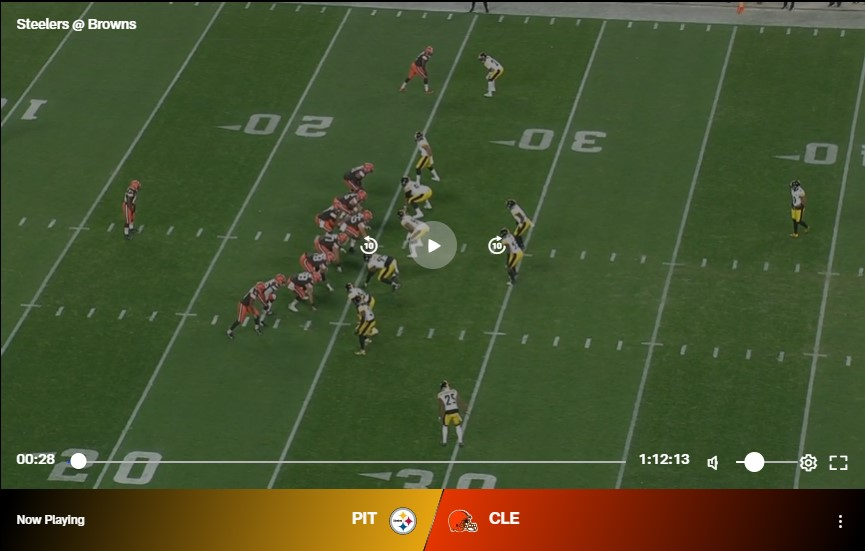
\includegraphics{images/all-22-screenshot.jpg}

}

\caption{Steelers vs.~Browns: 6 Offensive Linemen}

\end{figure}

In the second case, Dallas' offense personnel on its ``first play'' from
scrimmage is the result of the Cowboys returning a fumble for a
touchdown on the Rams' first offensive possession with a botched snap on
the ensuing extra point attempt. Because of that, the extra point
attempt is no longer scored as an \texttt{extra\_point} in the
\texttt{play\_type} variable within the play-by-play data, but a rushing
attempt. As a result of this oddity, the data is correct in listing
Dallas' first offensive play as coming out of an extra point personnel
grouping.

Both of these examples are problematic as a team's ``starting offensive
line'' is considered to be just five players: the left tackle, the left
guard, the center, the right guard, and the right tackle. In order to
correctly determine the number of combinations used, we need to first
determine the five most-commonly used offensive linemen for each team.
Because of the off-the-wall situations that can occur in football,
building offensive line combinations through personnel groupings in the
play-by--play data is tricky, at best.

To avoid these situations, we can turn to the
\texttt{load\_snap\_counts()} function with the \texttt{nflreadr}
package to determine the number of unique offensive line combinations.
The process to do so occurs over several steps and involves
decision-making on our end on how best to accurately represent the five
core offensive linemen for each team.

\begin{Shaded}
\begin{Highlighting}[]
\NormalTok{oline\_snap\_counts }\OtherTok{\textless{}{-}}\NormalTok{ nflreadr}\SpecialCharTok{::}\FunctionTok{load\_snap\_counts}\NormalTok{(}\AttributeTok{seasons =} \DecValTok{2022}\NormalTok{)}

\NormalTok{oline\_snap\_counts }\OtherTok{\textless{}{-}}\NormalTok{ oline\_snap\_counts }\SpecialCharTok{\%\textgreater{}\%}
  \FunctionTok{select}\NormalTok{(game\_id, week, player, position, team, offense\_pct) }\SpecialCharTok{\%\textgreater{}\%}
  \FunctionTok{filter}\NormalTok{(position }\SpecialCharTok{\%in\%} \FunctionTok{c}\NormalTok{(}\StringTok{"T"}\NormalTok{, }\StringTok{"G"}\NormalTok{, }\StringTok{"C"}\NormalTok{)) }\SpecialCharTok{\%\textgreater{}\%}
  \FunctionTok{group\_by}\NormalTok{(game\_id, team) }\SpecialCharTok{\%\textgreater{}\%}
  \FunctionTok{arrange}\NormalTok{(}\SpecialCharTok{{-}}\NormalTok{offense\_pct) }\SpecialCharTok{\%\textgreater{}\%}
\NormalTok{  dplyr}\SpecialCharTok{::}\FunctionTok{slice}\NormalTok{(}\DecValTok{1}\SpecialCharTok{:}\DecValTok{5}\NormalTok{) }\SpecialCharTok{\%\textgreater{}\%}
  \FunctionTok{ungroup}\NormalTok{()}

\NormalTok{oline\_snap\_counts}
\end{Highlighting}
\end{Shaded}

\begin{verbatim}
# A tibble: 2,840 x 6
   game_id          week player             position team  offense_pct
   <chr>           <int> <chr>              <chr>    <chr>       <dbl>
 1 2022_01_BAL_NYJ     1 Ben Powers         G        BAL          1   
 2 2022_01_BAL_NYJ     1 Morgan Moses       T        BAL          1   
 3 2022_01_BAL_NYJ     1 Kevin Zeitler      G        BAL          1   
 4 2022_01_BAL_NYJ     1 Tyler Linderbaum   C        BAL          1   
 5 2022_01_BAL_NYJ     1 Patrick Mekari     G        BAL          0.57
 6 2022_01_BAL_NYJ     1 Max Mitchell       T        NYJ          1   
 7 2022_01_BAL_NYJ     1 Laken Tomlinson    G        NYJ          1   
 8 2022_01_BAL_NYJ     1 Alijah Vera-Tucker G        NYJ          1   
 9 2022_01_BAL_NYJ     1 George Fant        T        NYJ          1   
10 2022_01_BAL_NYJ     1 Connor McGovern    C        NYJ          1   
# ... with 2,830 more rows
\end{verbatim}

First, we obtain snap count data from the 2022 season and write it into
a data frame titled \texttt{oline\_snap\_counts}. After, we select just
the necessary columns and then filter out the \texttt{position}
information to include only tackles, guards, and centers. After grouping
each individual offensive line by \texttt{game\_id} and his respective
\texttt{team}, we arrange each player's snap count in descending order
using \texttt{offense\_pct}.

And this is where a decision needs to be made on how to best construct
the five starting offensive linemen for each team. By including
\texttt{slice(1:5)}, we are essentially selecting \emph{just} the five
offensive linemen with the most snap counts in that singular game.

Are these five plays necessarily the same five that started the game as
the two tackles, two guards, and one center? Perhaps not. But,
hypothetically, a team's starting center could have been injured a
series or two into the game and the second-string center played the bulk
of the snaps in that game.

Because of such situations, we can make the argument that the five
offensive line players with the highest percentage of snap counts for
each unique \texttt{game\_id} are to be considered the combination of
players used most often in that game.

Next, let's make the decision to arrange each team's offensive line, by
game, in alphabetical order. Since we do not have a reliable way to
include \emph{specific} offensive line positions (that is, we have
\emph{just} tackle instead of \emph{left} tackle or \emph{right}
tackle), we can build our combination numbers strictly based on the five
downed linemen, regardless of specific position on the line of
scrimmage.

After, we use the \texttt{toString()} function to place all five names
into a single column (\texttt{starting\_line}) and then filter out the
data to include just one \texttt{game\_id} for the linemen.

\begin{Shaded}
\begin{Highlighting}[]
\NormalTok{oline\_snap\_counts }\OtherTok{\textless{}{-}}\NormalTok{ oline\_snap\_counts }\SpecialCharTok{\%\textgreater{}\%}
  \FunctionTok{group\_by}\NormalTok{(game\_id, team) }\SpecialCharTok{\%\textgreater{}\%}
  \FunctionTok{arrange}\NormalTok{(player, }\AttributeTok{.by\_group =} \ConstantTok{TRUE}\NormalTok{)}

\NormalTok{oline\_final\_data }\OtherTok{\textless{}{-}}\NormalTok{ oline\_snap\_counts }\SpecialCharTok{\%\textgreater{}\%}
  \FunctionTok{group\_by}\NormalTok{(game\_id, week, team) }\SpecialCharTok{\%\textgreater{}\%}
  \FunctionTok{mutate}\NormalTok{(}\AttributeTok{starting\_line =} \FunctionTok{toString}\NormalTok{(player)) }\SpecialCharTok{\%\textgreater{}\%}
  \FunctionTok{select}\NormalTok{(game\_id, week, team, starting\_line) }\SpecialCharTok{\%\textgreater{}\%}
  \FunctionTok{distinct}\NormalTok{(game\_id, }\AttributeTok{.keep\_all =} \ConstantTok{TRUE}\NormalTok{)}
\end{Highlighting}
\end{Shaded}

The end result includes the \texttt{game\_id}, the \texttt{week}, the
\texttt{team} abbreviation, and the \texttt{starting\_line} column that
includes the names of the five offensive line players with the highest
snap count percentage for that specific game.

\begin{verbatim}
# A tibble: 568 x 4
# Groups:   game_id, week, team [568]
   game_id          week team  starting_line                                    
   <chr>           <int> <chr> <chr>                                            
 1 2022_01_BAL_NYJ     1 BAL   Ben Powers, Kevin Zeitler, Morgan Moses, Patrick~
 2 2022_01_BAL_NYJ     1 NYJ   Alijah Vera-Tucker, Connor McGovern, George Fant~
 3 2022_01_BUF_LA      1 BUF   Dion Dawkins, Mitch Morse, Rodger Saffold, Ryan ~
 4 2022_01_BUF_LA      1 LA    Brian Allen, Coleman Shelton, David Edwards, Jos~
 5 2022_01_CLE_CAR     1 CAR   Austin Corbett, Brady Christensen, Ikem Ekwonu, ~
 6 2022_01_CLE_CAR     1 CLE   Ethan Pocic, James Hudson, Jedrick Wills Jr., Jo~
 7 2022_01_DEN_SEA     1 DEN   Cameron Fleming, Dalton Risner, Garett Bolles, G~
 8 2022_01_DEN_SEA     1 SEA   Abraham Lucas, Austin Blythe, Charles Cross, Gab~
 9 2022_01_GB_MIN      1 GB    Jake Hanson, Jon Runyan, Josh Myers, Royce Newma~
10 2022_01_GB_MIN      1 MIN   Brian O'Neill, Christian Darrisaw, Ed Ingram, Ez~
# ... with 558 more rows
\end{verbatim}

With the data cleaned and prepared, we are now able to take our first
look at the results. In the code below, we are grouping by all 32 NFL
team and then summarizing the total number of unique offensive line
combinations used during the 2022 regular season.

\begin{Shaded}
\begin{Highlighting}[]
\NormalTok{total\_combos }\OtherTok{\textless{}{-}}\NormalTok{ oline\_final\_data }\SpecialCharTok{\%\textgreater{}\%}
  \FunctionTok{group\_by}\NormalTok{(team) }\SpecialCharTok{\%\textgreater{}\%}
  \FunctionTok{summarize}\NormalTok{(}\AttributeTok{combos =} \FunctionTok{n\_distinct}\NormalTok{(starting\_line)) }\SpecialCharTok{\%\textgreater{}\%}
  \FunctionTok{arrange}\NormalTok{(}\SpecialCharTok{{-}}\NormalTok{combos)}
\end{Highlighting}
\end{Shaded}

Despite much of the media focus being on the Rams' poor performance,
given their title of defending Super Bowl Champions, the Arizona
Cardinals had nearly as many unique offensive line combinations at the
conclusion of the season.

With the data cleaned and prepared, let's use it to create a
\texttt{ggplot} graph and compare the relationship between a team's
number of unique offensive lines against its winning percentage. To
complete this, we first need to join the winning percentages to our
existing \texttt{total\_combos} data frame.

\hypertarget{unique-offensive-line-combinations-vs.-win-percentage}{%
\subsection{Unique Offensive Line Combinations vs.~Win
Percentage}\label{unique-offensive-line-combinations-vs.-win-percentage}}

To bring in the individual winning percentages, we will use the
\texttt{get\_nfl\_standings()} function from \texttt{espnscrapeR} and
then combine the two sets of data on team abbreviations via a
\texttt{left\_join()}. Unfortunately, the team abbreviation returned
from \texttt{espnscrapeR} does not match up with those used in the
\texttt{nflverse} for both the Los Angeles Rams and the Washington
Commanders (LAR vs.~LA and WSH vs.~WAS). As evidenced in the below code,
correcting this issue is simple with the \texttt{clean\_team\_abbrs()}
function in the \texttt{nflreadr} package.

\begin{Shaded}
\begin{Highlighting}[]
\NormalTok{records }\OtherTok{\textless{}{-}}\NormalTok{ espnscrapeR}\SpecialCharTok{::}\FunctionTok{get\_nfl\_standings}\NormalTok{(}\AttributeTok{season =} \DecValTok{2022}\NormalTok{) }\SpecialCharTok{\%\textgreater{}\%}
  \FunctionTok{select}\NormalTok{(team\_abb, win\_pct)}
\end{Highlighting}
\end{Shaded}

\begin{verbatim}
Returning 2022
\end{verbatim}

\begin{Shaded}
\begin{Highlighting}[]
\NormalTok{records}\SpecialCharTok{$}\NormalTok{team\_abb }\OtherTok{\textless{}{-}}\NormalTok{ nflreadr}\SpecialCharTok{::}\FunctionTok{clean\_team\_abbrs}\NormalTok{(records}\SpecialCharTok{$}\NormalTok{team\_abb)}

\NormalTok{total\_combos }\OtherTok{\textless{}{-}}\NormalTok{ total\_combos }\SpecialCharTok{\%\textgreater{}\%}
  \FunctionTok{left\_join}\NormalTok{(records, }\AttributeTok{by =} \FunctionTok{c}\NormalTok{(}\StringTok{"team"} \OtherTok{=} \StringTok{"team\_abb"}\NormalTok{))}

\NormalTok{total\_combos}
\end{Highlighting}
\end{Shaded}

\begin{verbatim}
# A tibble: 32 x 3
   team  combos win_pct
   <chr>  <int>   <dbl>
 1 LA        13   0.294
 2 ARI       12   0.235
 3 CHI       10   0.176
 4 WAS       10   0.5  
 5 DEN        9   0.294
 6 NO         9   0.412
 7 NYJ        9   0.412
 8 GB         8   0.471
 9 TB         8   0.471
10 BUF        7   0.812
# ... with 22 more rows
\end{verbatim}

After collecting team records and merging them into the offensive line
combination data, we can use \texttt{ggplot} to visualize the data.
Individual team logos are used in place of the typical
\texttt{geom\_point} by using the \texttt{nflplotR} package.

\begin{tcolorbox}[enhanced jigsaw, left=2mm, toprule=.15mm, opacitybacktitle=0.6, leftrule=.75mm, bottomrule=.15mm, colbacktitle=quarto-callout-important-color!10!white, breakable, colback=white, bottomtitle=1mm, toptitle=1mm, title=\textcolor{quarto-callout-important-color}{\faExclamation}\hspace{0.5em}{Important}, coltitle=black, titlerule=0mm, arc=.35mm, opacityback=0, colframe=quarto-callout-important-color-frame, rightrule=.15mm]

Please note in the below \texttt{ggplot} coding that we are using a
custom theme, \texttt{nfl\_analytics\_theme()}. If you wish to replicate
the below visualization using the theme, run the below code to place the
theme into your RStudio environment allowing you to call it within
\texttt{ggplot}. Be sure to install and run the \texttt{ggtext} package
as the theme uses the package's \texttt{element\_markdown()} function.

\end{tcolorbox}

\begin{Shaded}
\begin{Highlighting}[]
\NormalTok{nfl\_analytics\_theme }\OtherTok{\textless{}{-}} \ControlFlowTok{function}\NormalTok{(..., }\AttributeTok{base\_size =} \DecValTok{12}\NormalTok{) \{}
  
  \FunctionTok{theme}\NormalTok{(}
    \AttributeTok{text =} \FunctionTok{element\_text}\NormalTok{(}\AttributeTok{family =} \StringTok{"Roboto"}\NormalTok{,}
                        \AttributeTok{size =}\NormalTok{ base\_size,}
                        \AttributeTok{color =} \StringTok{"black"}\NormalTok{),}
    \AttributeTok{axis.ticks =} \FunctionTok{element\_blank}\NormalTok{(),}
    \AttributeTok{axis.title =} \FunctionTok{element\_text}\NormalTok{(}\AttributeTok{face =} \StringTok{"bold"}\NormalTok{),}
    \AttributeTok{axis.text =} \FunctionTok{element\_text}\NormalTok{(}\AttributeTok{face =} \StringTok{"bold"}\NormalTok{),}
    \AttributeTok{plot.title.position =} \StringTok{"plot"}\NormalTok{,}
    \AttributeTok{plot.title =} \FunctionTok{element\_markdown}\NormalTok{(}\AttributeTok{size =} \DecValTok{16}\NormalTok{,}
                                  \AttributeTok{vjust =}\NormalTok{ .}\DecValTok{02}\NormalTok{,}
                                  \AttributeTok{hjust =} \FloatTok{0.5}\NormalTok{),}
    \AttributeTok{plot.subtitle =} \FunctionTok{element\_markdown}\NormalTok{(}\AttributeTok{hjust =} \FloatTok{0.5}\NormalTok{),}
    \AttributeTok{plot.caption =} \FunctionTok{element\_markdown}\NormalTok{(}\AttributeTok{size =} \DecValTok{8}\NormalTok{),}
    \AttributeTok{panel.grid.minor =} \FunctionTok{element\_blank}\NormalTok{(),}
    \AttributeTok{panel.grid.major =}  \FunctionTok{element\_line}\NormalTok{(}\AttributeTok{color =} \StringTok{"\#d0d0d0"}\NormalTok{),}
    \AttributeTok{panel.background =} \FunctionTok{element\_rect}\NormalTok{(}\AttributeTok{fill =} \StringTok{"\#f7f7f7"}\NormalTok{),}
    \AttributeTok{plot.background =} \FunctionTok{element\_rect}\NormalTok{(}\AttributeTok{fill =} \StringTok{"\#f7f7f7"}\NormalTok{),}
    \AttributeTok{panel.border =} \FunctionTok{element\_blank}\NormalTok{(),}
    \AttributeTok{legend.background =} \FunctionTok{element\_rect}\NormalTok{(}\AttributeTok{color =} \StringTok{"\#F7F7F7"}\NormalTok{),}
    \AttributeTok{legend.key =} \FunctionTok{element\_rect}\NormalTok{(}\AttributeTok{color =} \StringTok{"\#F7F7F7"}\NormalTok{),}
    \AttributeTok{legend.title =} \FunctionTok{element\_text}\NormalTok{(}\AttributeTok{face =} \StringTok{"bold"}\NormalTok{),}
    \AttributeTok{legend.title.align =} \FloatTok{0.5}\NormalTok{,}
    \AttributeTok{strip.text =} \FunctionTok{element\_text}\NormalTok{(}\AttributeTok{face =} \StringTok{"bold"}\NormalTok{))}
\NormalTok{\}}
\end{Highlighting}
\end{Shaded}

\begin{Shaded}
\begin{Highlighting}[]
\FunctionTok{ggplot}\NormalTok{(}\AttributeTok{data =}\NormalTok{ total\_combos, }\FunctionTok{aes}\NormalTok{(}\AttributeTok{x =}\NormalTok{ combos, }\AttributeTok{y =}\NormalTok{ win\_pct)) }\SpecialCharTok{+}
  \FunctionTok{geom\_line}\NormalTok{(}\AttributeTok{stat =} \StringTok{"smooth"}\NormalTok{, }\AttributeTok{method =} \StringTok{"lm"}\NormalTok{,}
            \AttributeTok{size =}\NormalTok{ .}\DecValTok{7}\NormalTok{, }\AttributeTok{color =} \StringTok{"blue"}\NormalTok{,}
            \AttributeTok{alpha =} \FloatTok{0.25}\NormalTok{) }\SpecialCharTok{+}
\NormalTok{  nflplotR}\SpecialCharTok{::}\FunctionTok{geom\_mean\_lines}\NormalTok{(}\FunctionTok{aes}\NormalTok{(}\AttributeTok{v\_var =}\NormalTok{ combos, }\AttributeTok{h\_var =}\NormalTok{ win\_pct),}
                            \AttributeTok{color =} \StringTok{"black"}\NormalTok{, }\AttributeTok{size =}\NormalTok{ .}\DecValTok{8}\NormalTok{) }\SpecialCharTok{+}
\NormalTok{  nflplotR}\SpecialCharTok{::}\FunctionTok{geom\_nfl\_logos}\NormalTok{(}\FunctionTok{aes}\NormalTok{(}\AttributeTok{team\_abbr =}\NormalTok{ team), }\AttributeTok{width =} \FloatTok{0.065}\NormalTok{) }\SpecialCharTok{+}
  \FunctionTok{scale\_x\_reverse}\NormalTok{(}\AttributeTok{breaks =}\NormalTok{ scales}\SpecialCharTok{::}\FunctionTok{pretty\_breaks}\NormalTok{(}\AttributeTok{n =} \DecValTok{12}\NormalTok{)) }\SpecialCharTok{+}
  \FunctionTok{scale\_y\_continuous}\NormalTok{(}\AttributeTok{breaks =}\NormalTok{ scales}\SpecialCharTok{::}\FunctionTok{pretty\_breaks}\NormalTok{(}\AttributeTok{n =} \DecValTok{6}\NormalTok{),}
                     \AttributeTok{labels =}\NormalTok{ scales}\SpecialCharTok{::}\FunctionTok{label\_number}\NormalTok{(}\AttributeTok{accuracy =} \FloatTok{0.001}\NormalTok{)) }\SpecialCharTok{+}
  \FunctionTok{nfl\_analytics\_theme}\NormalTok{() }\SpecialCharTok{+}
  \FunctionTok{xlab}\NormalTok{(}\StringTok{"\# of Unique Offensive Line Combinations"}\NormalTok{) }\SpecialCharTok{+}
  \FunctionTok{ylab}\NormalTok{(}\StringTok{"Win Percentage"}\NormalTok{) }\SpecialCharTok{+}
  \FunctionTok{labs}\NormalTok{(}\AttributeTok{title =} \StringTok{"**Unique Offensive Line Combinations vs. Win Percentage**"}\NormalTok{,}
       \AttributeTok{subtitle =} \StringTok{"*Through Week \#15*"}\NormalTok{,}
       \AttributeTok{caption =} \StringTok{"*An Introduction to NFL Analytics With R*\textless{}br\textgreater{}**Brad J. Congelio**"}\NormalTok{)}
\end{Highlighting}
\end{Shaded}

\begin{verbatim}
Warning: Using `size` aesthetic for lines was deprecated in ggplot2 3.4.0.
i Please use `linewidth` instead.
\end{verbatim}

\begin{verbatim}
`geom_smooth()` using formula = 'y ~ x'
\end{verbatim}

\begin{verbatim}
Warning: Using the `size` aesthetic with geom_segment was deprecated in ggplot2 3.4.0.
i Please use the `linewidth` aesthetic instead.
\end{verbatim}

\begin{figure}[H]

{\centering 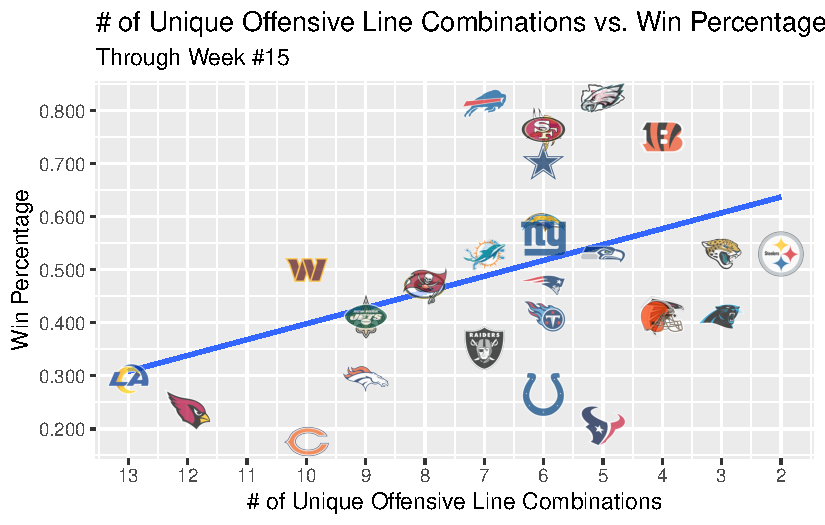
\includegraphics{01-nfl-analytics-and-r_files/figure-pdf/plot-combos-1.pdf}

}

\end{figure}

As can be seen in the resulting graph - which shows little, if any,
statistical correlation - there are still teams with worse records than
the Rams and Cardinals that have fewer unique offensive line
combinations (the Houston Texans and the Chicago Bears, for example).
Perhaps there is a metric that correlates more strongly with a team's
number of offensive line combinations?

To begin exploring that, we can hypothesize that more offensive line
combinations leads to more quarterback pressures as the various member
of the offensive line never have time to properly ``gel.''

\hypertarget{unique-offensive-line-combinations-vs.-pressure-rate}{%
\subsection{Unique Offensive Line Combinations vs.~Pressure
Rate}\label{unique-offensive-line-combinations-vs.-pressure-rate}}

Rather than calculate the data ourselves (which is the total number
dropbacks divided by the total number of pressures), we can turn away
from \texttt{nflverse} data and retrieve the information from the
\href{https://pro.sisdatahub.com/}{SIS Data Hub}. After downloading the
spreadsheet, we can read it into the RStudio environment using
\texttt{vroom} and then merge the information into the existing
\texttt{total\_combos} data frame by matching on the individual team
abbreviations.

\begin{Shaded}
\begin{Highlighting}[]
\NormalTok{pressure\_rate }\OtherTok{\textless{}{-}} \FunctionTok{vroom}\NormalTok{(}\StringTok{"./example\_data/csv/ch1\_pressurerate.csv"}\NormalTok{)}

\NormalTok{total\_combos }\OtherTok{\textless{}{-}}\NormalTok{ total\_combos }\SpecialCharTok{\%\textgreater{}\%}
  \FunctionTok{left\_join}\NormalTok{(pressure\_rate, }\AttributeTok{by =} \FunctionTok{c}\NormalTok{(}\StringTok{"team"} \OtherTok{=} \StringTok{"team\_abbr"}\NormalTok{))}
\end{Highlighting}
\end{Shaded}

\begin{verbatim}
# A tibble: 32 x 5
   team  combos win_pct season pressure_percent
   <chr>  <int>   <dbl>  <dbl>            <dbl>
 1 LA        13   0.294   2022             34.7
 2 ARI       12   0.235   2022             26.5
 3 CHI       10   0.176   2022             42.3
 4 WAS       10   0.5     2022             38.4
 5 DEN        9   0.294   2022             33.8
 6 NO         9   0.412   2022             28.2
 7 NYJ        9   0.412   2022             33.9
 8 GB         8   0.471   2022             25.4
 9 TB         8   0.471   2022             19.6
10 BUF        7   0.812   2022             31.8
# ... with 22 more rows
\end{verbatim}

With the pressure rate now merged with our unique offensive line
combination data, we can make slight adjustments to our prior
\texttt{ggplot} code to examine any potential relationship.

\begin{Shaded}
\begin{Highlighting}[]
\FunctionTok{ggplot}\NormalTok{(}\AttributeTok{data =}\NormalTok{ total\_combos, }\FunctionTok{aes}\NormalTok{(}\AttributeTok{x =}\NormalTok{ combos, }\AttributeTok{y =}\NormalTok{ pressure\_percent)) }\SpecialCharTok{+}
  \FunctionTok{geom\_line}\NormalTok{(}\AttributeTok{stat =} \StringTok{"smooth"}\NormalTok{, }\AttributeTok{method =} \StringTok{"lm"}\NormalTok{,}
            \AttributeTok{size =}\NormalTok{ .}\DecValTok{7}\NormalTok{, }\AttributeTok{color =} \StringTok{"blue"}\NormalTok{,}
            \AttributeTok{alpha =} \FloatTok{0.25}\NormalTok{) }\SpecialCharTok{+}
\NormalTok{  nflplotR}\SpecialCharTok{::}\FunctionTok{geom\_mean\_lines}\NormalTok{(}\FunctionTok{aes}\NormalTok{(}\AttributeTok{v\_var =}\NormalTok{ combos, }\AttributeTok{h\_var =}\NormalTok{ pressure\_percent),}
                            \AttributeTok{color =} \StringTok{"black"}\NormalTok{, }\AttributeTok{size =}\NormalTok{ .}\DecValTok{8}\NormalTok{) }\SpecialCharTok{+}
\NormalTok{  nflplotR}\SpecialCharTok{::}\FunctionTok{geom\_nfl\_logos}\NormalTok{(}\FunctionTok{aes}\NormalTok{(}\AttributeTok{team\_abbr =}\NormalTok{ team), }\AttributeTok{width =} \FloatTok{0.065}\NormalTok{) }\SpecialCharTok{+}
  \FunctionTok{scale\_x\_reverse}\NormalTok{(}\AttributeTok{breaks =}\NormalTok{ scales}\SpecialCharTok{::}\FunctionTok{pretty\_breaks}\NormalTok{(}\AttributeTok{n =} \DecValTok{12}\NormalTok{)) }\SpecialCharTok{+}
  \FunctionTok{scale\_y\_reverse}\NormalTok{(}\AttributeTok{breaks =}\NormalTok{ scales}\SpecialCharTok{::}\FunctionTok{pretty\_breaks}\NormalTok{(}\AttributeTok{n =} \DecValTok{6}\NormalTok{),}
                     \AttributeTok{labels =}\NormalTok{ scales}\SpecialCharTok{::}\FunctionTok{percent\_format}\NormalTok{(}\AttributeTok{scale =} \DecValTok{1}\NormalTok{,}
                                                     \AttributeTok{accuracy =} \FloatTok{0.1}\NormalTok{)) }\SpecialCharTok{+}
  \FunctionTok{nfl\_analytics\_theme}\NormalTok{() }\SpecialCharTok{+}
  \FunctionTok{xlab}\NormalTok{(}\StringTok{"\# of Unique Offensive Line Combinations"}\NormalTok{) }\SpecialCharTok{+}
  \FunctionTok{ylab}\NormalTok{(}\StringTok{"Pressure Rate (per Dropback)"}\NormalTok{) }\SpecialCharTok{+}
  \FunctionTok{labs}\NormalTok{(}\AttributeTok{title =} \StringTok{"Unique Offensive Line Combinations vs. Pressure Rate"}\NormalTok{,}
       \AttributeTok{subtitle =} \StringTok{"2022 Season"}\NormalTok{,}
       \AttributeTok{caption =} \StringTok{"*An Introduction to NFL Analytics with R*\textless{}br\textgreater{}**Brad J. Congelio**"}\NormalTok{)}
\end{Highlighting}
\end{Shaded}

\begin{verbatim}
`geom_smooth()` using formula = 'y ~ x'
\end{verbatim}

\begin{figure}[H]

{\centering 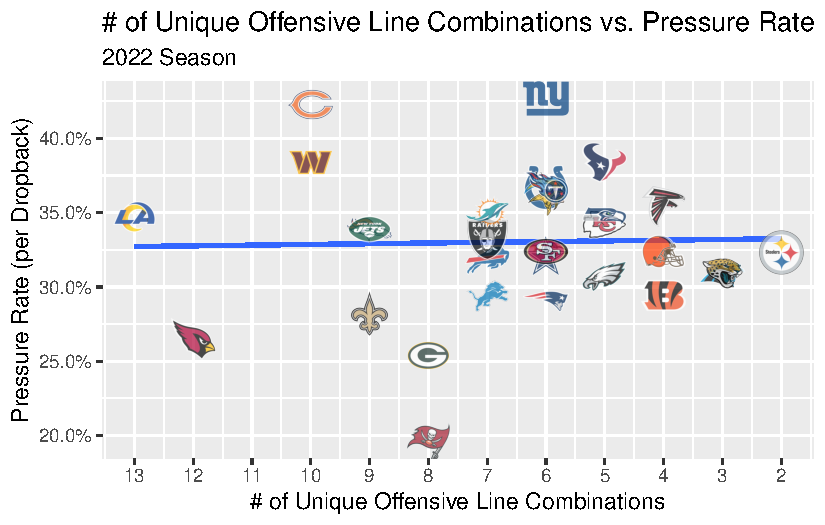
\includegraphics{01-nfl-analytics-and-r_files/figure-pdf/plot-pressure-rate-1.pdf}

}

\end{figure}

Again, there does not seem to be any statistical correlation between a
team's number of unique offensive line combinations and the pressure
rate per dropback allowed. Rather than examining the pressure per
dropback rate, perhaps there is a correlation between a the number of
unique offensive line combinations and the total number of quarterback
hits allowed through the season? To determine the validity of that
hypothesis, we can use data from \texttt{nflreadr} to collect total QB
hits.

\hypertarget{unique-offensive-line-combinations-vs.-qb-hits-allowed}{%
\subsection{Unique Offensive Line Combinations vs.~QB Hits
Allowed}\label{unique-offensive-line-combinations-vs.-qb-hits-allowed}}

To begin, we can collect the QB hit data from \texttt{nflreadr} being
sure to \texttt{group\_by()} the \texttt{posteam} variable in order to
calculate the number of QB hits allowed by each team's offensive line.
After, we can merge the data into the \texttt{total\_combos} data frame
and produce the plot.

\begin{Shaded}
\begin{Highlighting}[]
\NormalTok{pbp }\OtherTok{\textless{}{-}}\NormalTok{ nflreadr}\SpecialCharTok{::}\FunctionTok{load\_pbp}\NormalTok{(}\DecValTok{2022}\NormalTok{)}

\NormalTok{qb\_hits }\OtherTok{\textless{}{-}}\NormalTok{ pbp }\SpecialCharTok{\%\textgreater{}\%}
  \FunctionTok{filter}\NormalTok{(}\SpecialCharTok{!}\FunctionTok{is.na}\NormalTok{(posteam)) }\SpecialCharTok{\%\textgreater{}\%}
  \FunctionTok{group\_by}\NormalTok{(posteam) }\SpecialCharTok{\%\textgreater{}\%}
  \FunctionTok{summarize}\NormalTok{(}\AttributeTok{total\_qb\_hits =} \FunctionTok{sum}\NormalTok{(qb\_hit }\SpecialCharTok{==} \DecValTok{1}\NormalTok{, }\AttributeTok{na.rm =} \ConstantTok{TRUE}\NormalTok{))}

\NormalTok{qb\_hits\_combined }\OtherTok{\textless{}{-}} \FunctionTok{left\_join}\NormalTok{(}
\NormalTok{  total\_combos, qb\_hits, }\AttributeTok{by =} \FunctionTok{c}\NormalTok{(}\StringTok{"team"} \OtherTok{=} \StringTok{"posteam"}\NormalTok{))}
\end{Highlighting}
\end{Shaded}

After first filtering out any data that does not include
\texttt{posteam} information, we can \texttt{group\_by()} each
individual offensive unit and then calculate the total sum of QB hits
for each.

\begin{Shaded}
\begin{Highlighting}[]
\FunctionTok{ggplot}\NormalTok{(}\AttributeTok{data =}\NormalTok{ qb\_hits\_combined, }\FunctionTok{aes}\NormalTok{(}\AttributeTok{x =}\NormalTok{ combos, }\AttributeTok{y =}\NormalTok{ total\_qb\_hits)) }\SpecialCharTok{+}
    \FunctionTok{geom\_line}\NormalTok{(}\AttributeTok{stat =} \StringTok{"smooth"}\NormalTok{, }\AttributeTok{method =} \StringTok{"lm"}\NormalTok{,}
              \AttributeTok{size =}\NormalTok{ .}\DecValTok{7}\NormalTok{, }\AttributeTok{color =} \StringTok{"blue"}\NormalTok{,}
              \AttributeTok{alpha =} \FloatTok{0.25}\NormalTok{) }\SpecialCharTok{+}
\NormalTok{  nflplotR}\SpecialCharTok{::}\FunctionTok{geom\_mean\_lines}\NormalTok{(}\FunctionTok{aes}\NormalTok{(}\AttributeTok{v\_var =}\NormalTok{ combos, }\AttributeTok{h\_var =}\NormalTok{ total\_qb\_hits),}
                            \AttributeTok{color =} \StringTok{"black"}\NormalTok{, }\AttributeTok{size =}\NormalTok{ .}\DecValTok{8}\NormalTok{) }\SpecialCharTok{+}
\NormalTok{  nflplotR}\SpecialCharTok{::}\FunctionTok{geom\_nfl\_logos}\NormalTok{(}\FunctionTok{aes}\NormalTok{(}\AttributeTok{team\_abbr =}\NormalTok{ team), }\AttributeTok{width =} \FloatTok{0.065}\NormalTok{) }\SpecialCharTok{+}
  \FunctionTok{scale\_x\_reverse}\NormalTok{(}\AttributeTok{breaks =}\NormalTok{ scales}\SpecialCharTok{::}\FunctionTok{pretty\_breaks}\NormalTok{()) }\SpecialCharTok{+}
  \FunctionTok{scale\_y\_reverse}\NormalTok{(}\AttributeTok{breaks =}\NormalTok{ scales}\SpecialCharTok{::}\FunctionTok{pretty\_breaks}\NormalTok{()) }\SpecialCharTok{+}
  \FunctionTok{nfl\_analytics\_theme}\NormalTok{() }\SpecialCharTok{+}
  \FunctionTok{xlab}\NormalTok{(}\StringTok{"\# of Unique Offensive Line Combinations"}\NormalTok{) }\SpecialCharTok{+}
  \FunctionTok{ylab}\NormalTok{(}\StringTok{"Total QB Hits Allowed"}\NormalTok{) }\SpecialCharTok{+}
  \FunctionTok{labs}\NormalTok{(}\AttributeTok{title =} \StringTok{"Unique Offensive Line Combinations vs. QB Hits Allowed"}\NormalTok{,}
       \AttributeTok{subtitle =} \StringTok{"2022 Season"}\NormalTok{,}
       \AttributeTok{caption =} \StringTok{"*An Introduction to NFl Analytics with R*\textless{}br\textgreater{}**Brad J. Congelio**"}\NormalTok{)}
\end{Highlighting}
\end{Shaded}

\begin{verbatim}
`geom_smooth()` using formula = 'y ~ x'
\end{verbatim}

\begin{figure}[H]

{\centering 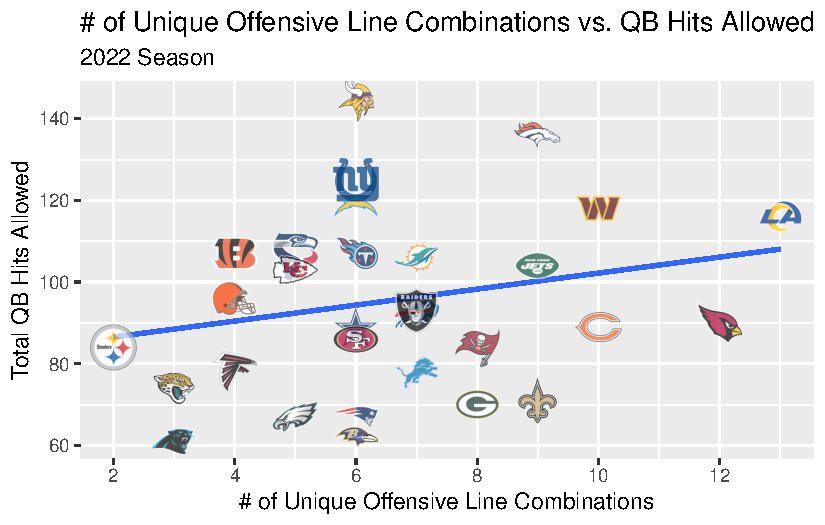
\includegraphics{01-nfl-analytics-and-r_files/figure-pdf/plot-combos-qb-hits-1.pdf}

}

\end{figure}

There is again very little, if any, correlation between a team's unique
number of offensive line combinations and the number of times its
quarterback is hit on passing attempts.

\hypertarget{unique-offensive-line-combinations-vs.-adjusted-sack-rate}{%
\subsection{Unique Offensive Line Combinations vs.~Adjusted Sack
Rate}\label{unique-offensive-line-combinations-vs.-adjusted-sack-rate}}

In the previous examples, both pressure rate and QB hits are unadjusted
metrics, meaning the results are not manipulated to account for context
within the data. To add an example of a metric that \emph{is} adjusted
to our list of examples, we will use Adjusted Sack Rate from
\href{https://www.footballoutsiders.com/}{Football Outsiders}. Aaron
Schatz, in an article introducing the measurements in December of 2003,
explained his findings that the league-wide sack rate varied based on
both the down and yards to go.

\begin{longtable}[]{@{}
  >{\centering\arraybackslash}p{(\columnwidth - 10\tabcolsep) * \real{0.2687}}
  >{\raggedright\arraybackslash}p{(\columnwidth - 10\tabcolsep) * \real{0.1343}}
  >{\raggedright\arraybackslash}p{(\columnwidth - 10\tabcolsep) * \real{0.1343}}
  >{\raggedright\arraybackslash}p{(\columnwidth - 10\tabcolsep) * \real{0.1493}}
  >{\raggedright\arraybackslash}p{(\columnwidth - 10\tabcolsep) * \real{0.1642}}
  >{\raggedright\arraybackslash}p{(\columnwidth - 10\tabcolsep) * \real{0.1493}}@{}}
\caption{2003 NFL Sack Rate - Aaron Schatz
(FootballOutsiders.com)}\tabularnewline
\toprule\noalign{}
\endfirsthead
\endhead
\bottomrule\noalign{}
\endlastfoot
\textbf{YARDS TO GO} & \textbf{1-4} & \textbf{5-8} & \textbf{9-12} &
\textbf{13-16} & \textbf{\textgreater17} \\
\textbf{1st Down} & \emph{1.5\%} & \emph{5.4\%} & \emph{4.8\%} &
\emph{3.3\%} & \emph{5.6\%} \\
\textbf{2nd Down} & \emph{5.6\%} & \emph{4.7\%} & \emph{5.0\%} &
\emph{6.1\%} & \emph{4.5\%} \\
\textbf{3rd/4th Down} & \emph{5.9\%} & \emph{8.2\%} & \emph{10.5\%} &
\emph{7.6\%} & \emph{11.1\%} \\
\end{longtable}

As a result of this, Schatz designed Adjusted Sack Rate which accounts
for the number of pass attempts, down, distance, and - importantly - the
team's opponent. We can plot the Adjusted Sack Rate for each team from
the 2022 season against the unique number of offensive line
combinations.

\begin{Shaded}
\begin{Highlighting}[]
\NormalTok{adjusted\_sack\_rate }\OtherTok{\textless{}{-}} 
  \FunctionTok{vroom}\NormalTok{(}\StringTok{"https://raw.githubusercontent.com/bcongelio/nfl{-}analytics{-}with{-}r{-}book/origin/example\_data/csv/adjusted\_sack\_rate.csv"}\NormalTok{)}
\end{Highlighting}
\end{Shaded}

\begin{Shaded}
\begin{Highlighting}[]
\NormalTok{adjusted\_sack\_rate }\SpecialCharTok{\%\textgreater{}\%}
  \FunctionTok{filter}\NormalTok{(season }\SpecialCharTok{==} \DecValTok{2022}\NormalTok{) }\SpecialCharTok{\%\textgreater{}\%}
  \FunctionTok{ggplot}\NormalTok{(}\FunctionTok{aes}\NormalTok{(}\AttributeTok{x =}\NormalTok{ combos, }\AttributeTok{y =}\NormalTok{ adj\_sack\_rate)) }\SpecialCharTok{+}
  \FunctionTok{geom\_line}\NormalTok{(}\AttributeTok{stat =} \StringTok{"smooth"}\NormalTok{, }\AttributeTok{method =} \StringTok{"lm"}\NormalTok{,}
            \AttributeTok{size =}\NormalTok{ .}\DecValTok{7}\NormalTok{,}
            \AttributeTok{color =} \StringTok{"blue"}\NormalTok{,}
            \AttributeTok{alpha =} \FloatTok{0.25}\NormalTok{) }\SpecialCharTok{+}
\NormalTok{  nflplotR}\SpecialCharTok{::}\FunctionTok{geom\_mean\_lines}\NormalTok{(}\FunctionTok{aes}\NormalTok{(}\AttributeTok{v\_var =}\NormalTok{ combos, }\AttributeTok{h\_var =}\NormalTok{ adj\_sack\_rate),}
                            \AttributeTok{color =} \StringTok{"black"}\NormalTok{, }\AttributeTok{size =}\NormalTok{ .}\DecValTok{8}\NormalTok{) }\SpecialCharTok{+}
\NormalTok{  nflplotR}\SpecialCharTok{::}\FunctionTok{geom\_nfl\_logos}\NormalTok{(}\FunctionTok{aes}\NormalTok{(}\AttributeTok{team\_abbr =}\NormalTok{ team), }\AttributeTok{width =} \FloatTok{0.065}\NormalTok{) }\SpecialCharTok{+}
  \FunctionTok{scale\_x\_reverse}\NormalTok{(}\AttributeTok{breaks =}\NormalTok{ scales}\SpecialCharTok{::}\FunctionTok{pretty\_breaks}\NormalTok{()) }\SpecialCharTok{+}
  \FunctionTok{scale\_y\_reverse}\NormalTok{(}\AttributeTok{breaks =}\NormalTok{ scales}\SpecialCharTok{::}\FunctionTok{pretty\_breaks}\NormalTok{(),}
                     \AttributeTok{labels =}\NormalTok{ scales}\SpecialCharTok{::}\FunctionTok{percent\_format}\NormalTok{(}\AttributeTok{scale =} \DecValTok{1}\NormalTok{)) }\SpecialCharTok{+}
  \FunctionTok{xlab}\NormalTok{(}\StringTok{"\# of Unique Offensive Line Combinations"}\NormalTok{) }\SpecialCharTok{+}
  \FunctionTok{ylab}\NormalTok{(}\StringTok{"Adjusted Sack Rate"}\NormalTok{) }\SpecialCharTok{+}
  \FunctionTok{labs}\NormalTok{(}\AttributeTok{title =} \StringTok{"**Unique Offensive Line Combinations vs. Adjusted Sack Rate**"}\NormalTok{,}
       \AttributeTok{subtitle =} \StringTok{"*2022 Season*"}\NormalTok{,}
       \AttributeTok{caption =} \StringTok{"*An Introduction to NFL Analytics with R*\textless{}br\textgreater{}**Brad J. Congelio**"}\NormalTok{) }\SpecialCharTok{+}
  \FunctionTok{nfl\_analytics\_theme}\NormalTok{()}
\end{Highlighting}
\end{Shaded}

\begin{verbatim}
`geom_smooth()` using formula = 'y ~ x'
\end{verbatim}

\begin{figure}[H]

{\centering 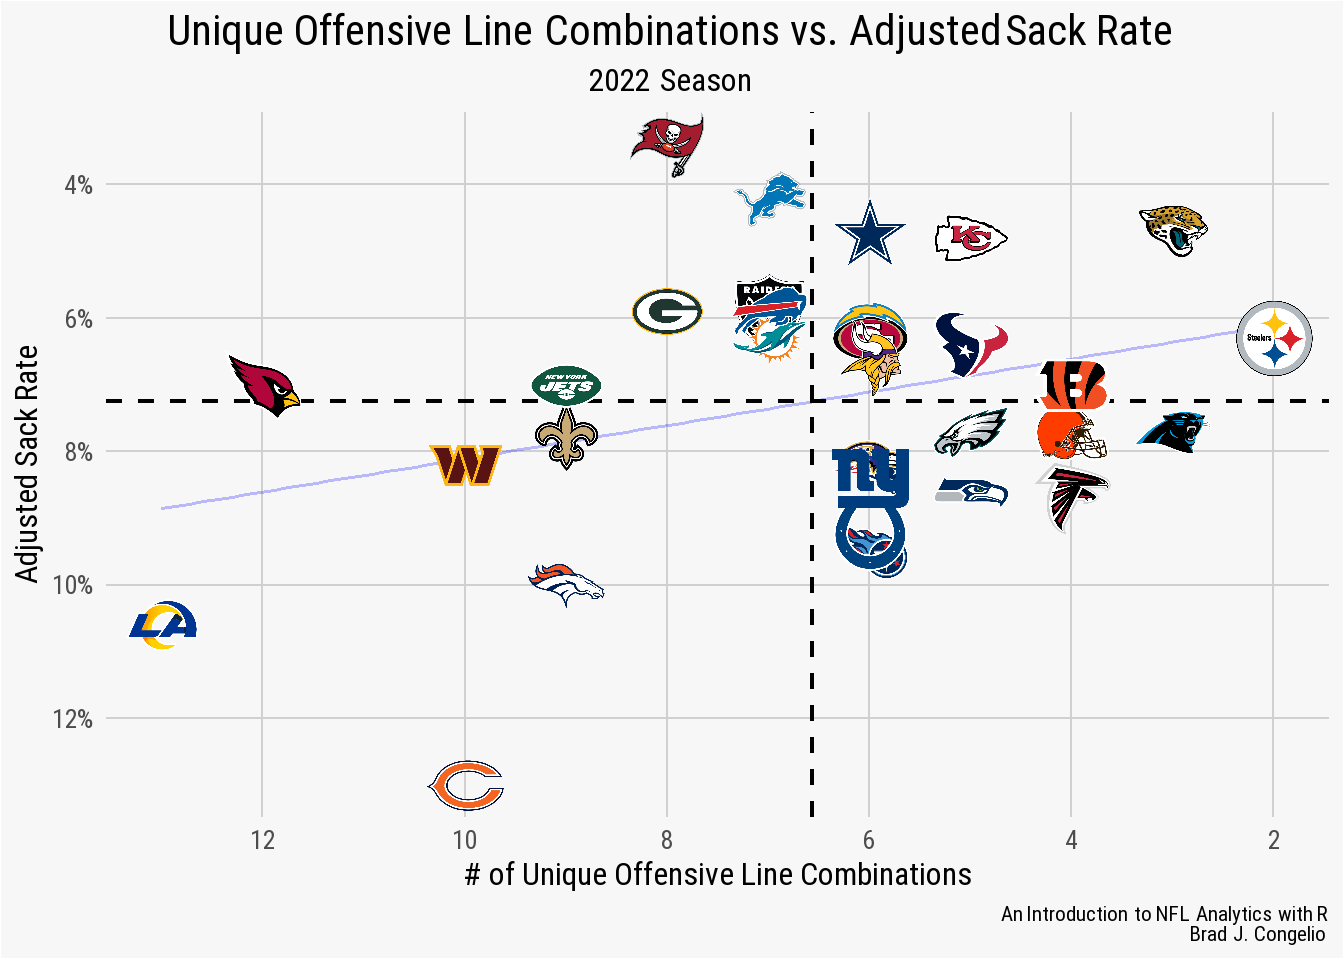
\includegraphics{01-nfl-analytics-and-r_files/figure-pdf/asr-2022-plot-1.pdf}

}

\end{figure}

The graph shows that, in general, those teams with higher numbers of
unique offensive line combinations trend towards the lower-left quadrant
and some - the Rams and Bears - are significantly below the league
average, indicating a worse adjusted sack rate (with the Arizona
Cardinals being an outlier). Compared to the prior metrics (pressure
rate and QB hits), it seems that adjusted sack rate may be impacted by
the consistency of a team's offensive linemen.

Using the \texttt{adjusted\_sack\_rate} data, we can easily visualize
the same results over the last three NFL seasons to see if there is any
consistency between the offensive line combinations and a team's
adjusted sack rate.

\begin{Shaded}
\begin{Highlighting}[]
\NormalTok{adjusted\_sack\_rate }\SpecialCharTok{\%\textgreater{}\%}
  \FunctionTok{ggplot}\NormalTok{(}\FunctionTok{aes}\NormalTok{(}\AttributeTok{x =}\NormalTok{ combos, }\AttributeTok{y =}\NormalTok{ adj\_sack\_rate)) }\SpecialCharTok{+}
  \FunctionTok{geom\_line}\NormalTok{(}\AttributeTok{stat =} \StringTok{"smooth"}\NormalTok{, }\AttributeTok{method =} \StringTok{"lm"}\NormalTok{,}
            \AttributeTok{size =}\NormalTok{ .}\DecValTok{7}\NormalTok{,}
            \AttributeTok{color =} \StringTok{"blue"}\NormalTok{,}
            \AttributeTok{alpha =} \FloatTok{0.25}\NormalTok{) }\SpecialCharTok{+}
\NormalTok{  nflplotR}\SpecialCharTok{::}\FunctionTok{geom\_mean\_lines}\NormalTok{(}\FunctionTok{aes}\NormalTok{(}\AttributeTok{v\_var =}\NormalTok{ combos, }\AttributeTok{h\_var =}\NormalTok{ adj\_sack\_rate),}
                            \AttributeTok{color =} \StringTok{"black"}\NormalTok{, }\AttributeTok{size =}\NormalTok{ .}\DecValTok{8}\NormalTok{) }\SpecialCharTok{+}
\NormalTok{  nflplotR}\SpecialCharTok{::}\FunctionTok{geom\_nfl\_logos}\NormalTok{(}\FunctionTok{aes}\NormalTok{(}\AttributeTok{team\_abbr =}\NormalTok{ team), }\AttributeTok{width =} \FloatTok{0.065}\NormalTok{) }\SpecialCharTok{+}
  \FunctionTok{scale\_x\_reverse}\NormalTok{(}\AttributeTok{breaks =}\NormalTok{ scales}\SpecialCharTok{::}\FunctionTok{pretty\_breaks}\NormalTok{()) }\SpecialCharTok{+}
  \FunctionTok{scale\_y\_reverse}\NormalTok{(}\AttributeTok{breaks =}\NormalTok{ scales}\SpecialCharTok{::}\FunctionTok{pretty\_breaks}\NormalTok{(),}
                  \AttributeTok{labels =}\NormalTok{ scales}\SpecialCharTok{::}\FunctionTok{percent\_format}\NormalTok{(}\AttributeTok{scale =} \DecValTok{1}\NormalTok{)) }\SpecialCharTok{+}
  \FunctionTok{xlab}\NormalTok{(}\StringTok{"\# of Unique Offensive Line Combinations"}\NormalTok{) }\SpecialCharTok{+}
  \FunctionTok{ylab}\NormalTok{(}\StringTok{"Adjusted Sack Rate"}\NormalTok{) }\SpecialCharTok{+}
  \FunctionTok{labs}\NormalTok{(}\AttributeTok{title =} \StringTok{"**Unique Offensive Line Combinations vs. Adjusted Sack Rate**"}\NormalTok{,}
       \AttributeTok{subtitle =} \StringTok{"*2020 {-} 2022 Seasons*"}\NormalTok{,}
       \AttributeTok{caption =} \StringTok{"*An Introduction to NFL Analytics with R*\textless{}br\textgreater{}**Brad J. Congelio**"}\NormalTok{) }\SpecialCharTok{+}
  \FunctionTok{nfl\_analytics\_theme}\NormalTok{() }\SpecialCharTok{+}
  \FunctionTok{facet\_wrap}\NormalTok{(}\SpecialCharTok{\textasciitilde{}}\NormalTok{season, }\AttributeTok{nrow =} \DecValTok{2}\NormalTok{)}
\end{Highlighting}
\end{Shaded}

\begin{verbatim}
`geom_smooth()` using formula = 'y ~ x'
\end{verbatim}

\begin{figure}[H]

{\centering 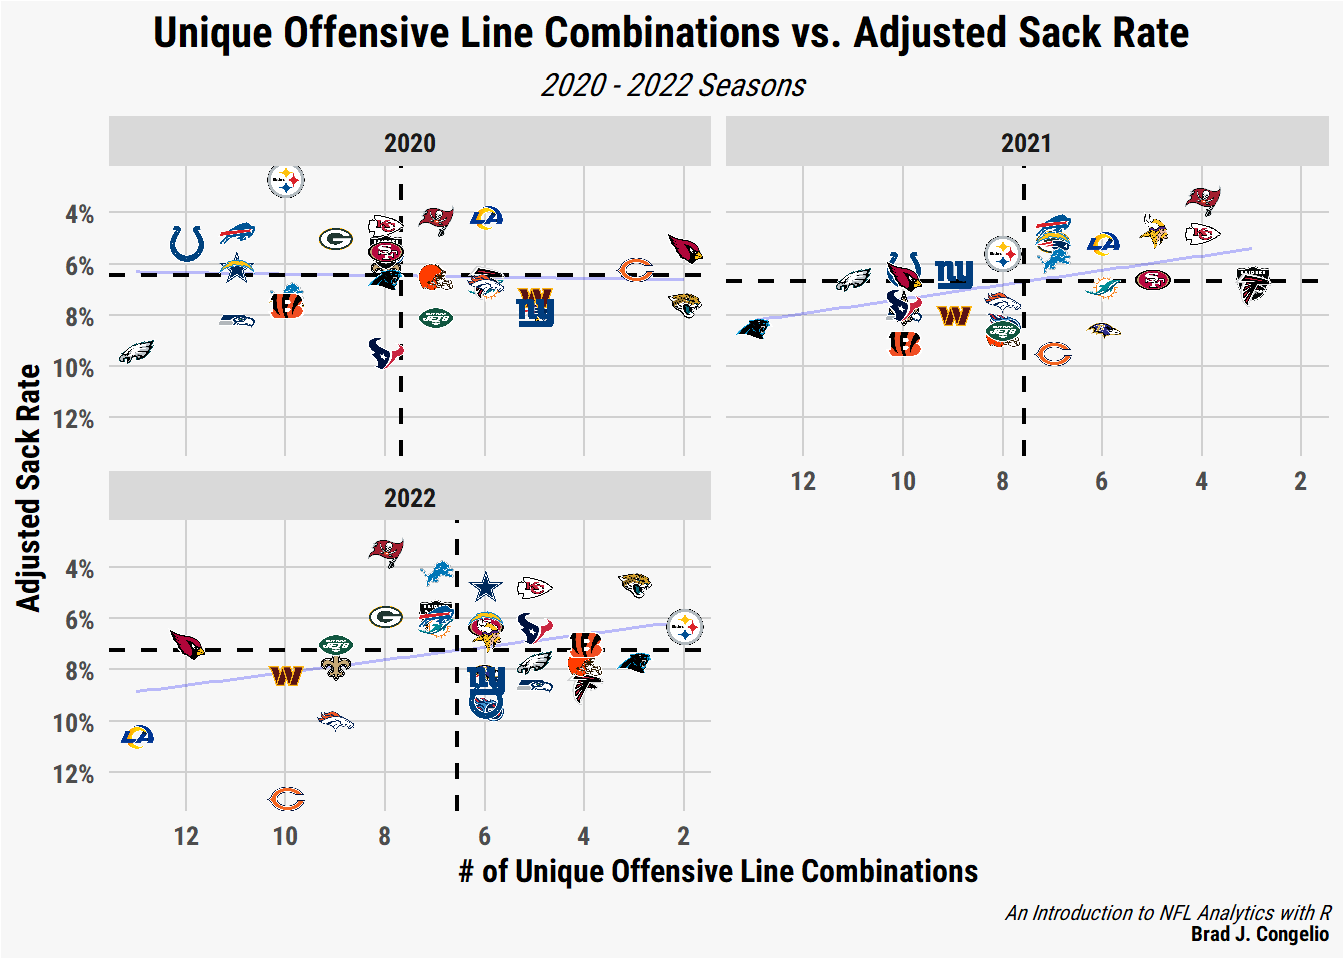
\includegraphics{01-nfl-analytics-and-r_files/figure-pdf/asr-facet-plot-1.pdf}

}

\end{figure}

Given the result of just the 2022 season, the output for the 2021 season
remains consistent, perhaps even more so with less spread from the line
of best fit. In 2021, the Carolina Panthers had the most unique
offensive line combinations as well as one of the worst adjusted sack
rates in the league, while those teams with fewer combinations generally
trend towards the upper-right quadrant of the plot.

However, the consistency between the 2022 and 2021 seasons is not found
in the 2020 season. The Philadelphia Eagles had the most unique
combinations in 2020 (13 in total), but were all but tied with the
Houston Texans for worst adjusted sack rate (9.4\% to 9.5\%). Moreover,
the Pittsburgh Steelers, Buffalo Bills, and Indianapolis Colts - despite
all having more than 10 unique offensive line combinations - are among
the best in adjusted sack rate.

Why is there this sudden departure from the consistency in 2022 and
2021?

The answer is within the context of data, in that Ben Roethlisberger -
the long-time quarterback for the Steelers - had one of the fastest Time
to Throw scores in modern NFL history, getting rid of the ball, on
average, in just 2.19 seconds after the snap. Philip Rivers, of the
Colts, was nearly as quick to release the ball with an average of 2.39
seconds. It proved to be quite difficult for opposing defenses to get to
either Roethlisberger or Rivers given these incredibly quick
snap-to-release times.

It should be noted that the same contextual explanation does not hold
true for Buffalo. In the 2020 season, Josh Allen released the ball, on
average, 3.04 seconds after the snap which is plenty of time for the
opposing defense to generate pressure and record sacks. Because of this,
if we were to add statistical weight using average time to throw, the
Buffalo Bills would remain an outlier in this specific season while both
the Steelers and Colts would likely regress closer to the mean for those
teams with higher numbers of offensive line combinations.

While pressure rate and QB hits did not prove to impacted by a team's
number of line combinations, there is a broad relationship (though not
strong enough to begin using the term ``correlation'') between the
number of combinations and adjusted sack rate.

To continue this exploration, let's pivot away from exploring the impact
of offensive line combinations on the quarterback and examine any
potential correlation with the running game and run blocking, while
using metrics that are adjusted, as the additional context and weighting
seemed to be helpful in finding relationships. We can gather statistics
provided by \href{https://www.footballoutsiders.com/}{Football
Outsiders} concerning the performance of offensive lines.

\hypertarget{unique-offensive-line-combinations-vs.-adjusted-line-yards}{%
\subsection{Unique Offensive Line Combinations vs.~Adjusted Line
Yards}\label{unique-offensive-line-combinations-vs.-adjusted-line-yards}}

\begin{enumerate}
\def\labelenumi{\arabic{enumi}.}
\tightlist
\item
  \textbf{Adjusted Line Yards} - derived by Football Outsiders with a
  regression analysis, this metric takes the total of a team's total
  rushing attempts and assigns a quantitative value to the offensive
  line's impact. Any run that ends with a loss of yards results in 120\%
  of the value being placed on the offensive line, while a 0-4 yard rush
  is 100\%, a 5-10 yard rush is 50\%, and anything over 11 yards is a
  0\% value. As explained by Football Outsiders, if a running back
  breaks free for a 50-yard gain, just how much of that is the offensive
  line responsible for? Adjusted Line Yards produces a numeric value as
  the answer to that question.
\item
  \textbf{Power Rank} - a ranking between 1 (best) and 32 (worst), power
  rank is the result of the power success metric, which is the
  percentage of rushing attempts on 3rd or 4th down, with two or less
  yards to go, that resulted in either a 1st down or a touchdown.
\item
  \textbf{Stuffed Rank} - again provided in the data frame as a ranking
  between 1 and 32, stuffed rank is the percentage of rushing attempts
  where the running back was tackled at, or behind, the line of
  scrimmage.
\end{enumerate}

To begin, we can gather the necessary data into a data frame called
\texttt{fb\_outsiders\_oline}.

\begin{Shaded}
\begin{Highlighting}[]
\NormalTok{fb\_outsiders\_oline }\OtherTok{\textless{}{-}}
  \FunctionTok{vroom}\NormalTok{(}\StringTok{"https://raw.githubusercontent.com/bcongelio/nfl{-}analytics{-}with{-}r{-}book/origin/example\_data/csv/fboutsiders\_line\_stats.csv"}\NormalTok{)}
\end{Highlighting}
\end{Shaded}

\begin{verbatim}
Rows: 32 Columns: 5
-- Column specification --------------------------------------------------------
Delimiter: ","
chr (1): team
dbl (4): combos, adj_line_yards, power_rank, stuffed_rank

i Use `spec()` to retrieve the full column specification for this data.
i Specify the column types or set `show_col_types = FALSE` to quiet this message.
\end{verbatim}

\begin{Shaded}
\begin{Highlighting}[]
\NormalTok{fb\_outsiders\_oline}
\end{Highlighting}
\end{Shaded}

\begin{verbatim}
# A tibble: 32 x 5
   team  combos adj_line_yards power_rank stuffed_rank
   <chr>  <dbl>          <dbl>      <dbl>        <dbl>
 1 LV         7           4.93         23            6
 2 GB         8           4.85         18            2
 3 KC         5           4.82         31            9
 4 SF         6           4.7          26           22
 5 ATL        4           4.68         17            5
 6 PHI        5           4.66          7            7
 7 DET        7           4.66         20           18
 8 MIA        7           4.61         30           14
 9 CAR        3           4.56         14           11
10 PIT        2           4.54          1            4
# ... with 22 more rows
\end{verbatim}

You can see in the output of the data that \texttt{power\_rank} and
\texttt{stuffed\_rank} are both in a ``ranked format,'' meaning the team
with the best power success score (the Pittsburgh Steelers) are ranked
1st while the team with the worst (the Minnesota Vikings) are ranked
32nd. The \texttt{adj\_line\_yards} variable is provided in its
unranked, raw format. Because of this, let's first use both
\texttt{power\_rank} and \texttt{stuffed\_rank} and use the
\texttt{cowplot} package to view them together, and then construct the
plot for \texttt{adj\_line\_yards} separately since it operates on a
differing y-axis scale.

\begin{Shaded}
\begin{Highlighting}[]
\NormalTok{power\_rank\_plot }\OtherTok{\textless{}{-}} \FunctionTok{ggplot}\NormalTok{(fb\_outsiders\_oline, }\FunctionTok{aes}\NormalTok{(}\AttributeTok{x =}\NormalTok{ combos, }\AttributeTok{y =}\NormalTok{ power\_rank)) }\SpecialCharTok{+}
\NormalTok{  nflplotR}\SpecialCharTok{::}\FunctionTok{geom\_mean\_lines}\NormalTok{(}\FunctionTok{aes}\NormalTok{(}\AttributeTok{v\_var =}\NormalTok{ combos, }\AttributeTok{h\_var =}\NormalTok{ power\_rank),}
                            \AttributeTok{color =} \StringTok{"black"}\NormalTok{,}
                            \AttributeTok{size =}\NormalTok{ .}\DecValTok{8}\NormalTok{) }\SpecialCharTok{+}
\NormalTok{  nflplotR}\SpecialCharTok{::}\FunctionTok{geom\_nfl\_logos}\NormalTok{(}\FunctionTok{aes}\NormalTok{(}\AttributeTok{team\_abbr =}\NormalTok{ team), }\AttributeTok{width =} \FloatTok{0.065}\NormalTok{) }\SpecialCharTok{+}
  \FunctionTok{scale\_x\_reverse}\NormalTok{(}\AttributeTok{breaks =}\NormalTok{ scales}\SpecialCharTok{::}\FunctionTok{pretty\_breaks}\NormalTok{()) }\SpecialCharTok{+}
  \FunctionTok{scale\_y\_reverse}\NormalTok{(}\AttributeTok{breaks =} \FunctionTok{seq}\NormalTok{(}\DecValTok{1}\NormalTok{, }\DecValTok{32}\NormalTok{, }\DecValTok{2}\NormalTok{)) }\SpecialCharTok{+}
  \FunctionTok{labs}\NormalTok{(}\AttributeTok{title =} \StringTok{"**Unique Offensive Line Combinations vs. Power Ranking**"}\NormalTok{,}
       \AttributeTok{subtitle =} \StringTok{"*2022 Season  |  FootballOutsiders.com*"}\NormalTok{,}
       \AttributeTok{caption =} \StringTok{"*An Introduction to NFL Analytics with R*\textless{}br\textgreater{}**Brad J. Congelio**"}\NormalTok{) }\SpecialCharTok{+}
  \FunctionTok{xlab}\NormalTok{(}\StringTok{"\# of Unique Offensive Line Combinations"}\NormalTok{) }\SpecialCharTok{+}
  \FunctionTok{ylab}\NormalTok{(}\StringTok{"Power Ranking (1 = best, 32 = worst)"}\NormalTok{) }\SpecialCharTok{+}
  \FunctionTok{nfl\_analytics\_theme}\NormalTok{()}

\NormalTok{stuffed\_rank\_plot }\OtherTok{\textless{}{-}} \FunctionTok{ggplot}\NormalTok{(fb\_outsiders\_oline, }\FunctionTok{aes}\NormalTok{(}\AttributeTok{x =}\NormalTok{ combos, }\AttributeTok{y =}\NormalTok{ stuffed\_rank)) }\SpecialCharTok{+}
  \FunctionTok{geom\_smooth}\NormalTok{(}\AttributeTok{method =} \StringTok{"lm"}\NormalTok{, }\AttributeTok{se =} \ConstantTok{FALSE}\NormalTok{, }\AttributeTok{size =} \FloatTok{0.8}\NormalTok{, }\AttributeTok{alpha =}\NormalTok{ .}\DecValTok{08}\NormalTok{) }\SpecialCharTok{+}
\NormalTok{  nflplotR}\SpecialCharTok{::}\FunctionTok{geom\_mean\_lines}\NormalTok{(}\FunctionTok{aes}\NormalTok{(}\AttributeTok{v\_var =}\NormalTok{ combos, }\AttributeTok{h\_var =}\NormalTok{ stuffed\_rank),}
                            \AttributeTok{color =} \StringTok{"black"}\NormalTok{,}
                            \AttributeTok{size =}\NormalTok{ .}\DecValTok{8}\NormalTok{) }\SpecialCharTok{+}
\NormalTok{  nflplotR}\SpecialCharTok{::}\FunctionTok{geom\_nfl\_logos}\NormalTok{(}\FunctionTok{aes}\NormalTok{(}\AttributeTok{team\_abbr =}\NormalTok{ team), }\AttributeTok{width =} \FloatTok{0.065}\NormalTok{) }\SpecialCharTok{+}
  \FunctionTok{scale\_x\_reverse}\NormalTok{(}\AttributeTok{breaks =}\NormalTok{ scales}\SpecialCharTok{::}\FunctionTok{pretty\_breaks}\NormalTok{()) }\SpecialCharTok{+}
  \FunctionTok{scale\_y\_reverse}\NormalTok{(}\AttributeTok{breaks =} \FunctionTok{seq}\NormalTok{(}\DecValTok{1}\NormalTok{, }\DecValTok{32}\NormalTok{, }\DecValTok{2}\NormalTok{)) }\SpecialCharTok{+}
  \FunctionTok{labs}\NormalTok{(}\AttributeTok{title =} \StringTok{"**Unique Offensive Line Combinations vs. Stuffed Rank**"}\NormalTok{,}
       \AttributeTok{subtitle =} \StringTok{"*2022 Season  |  FootballOutsiders.com*"}\NormalTok{,}
       \AttributeTok{caption =} \StringTok{"*An Introduction to NFL Analytics with R*\textless{}br\textgreater{}**Brad J. Congelio**"}\NormalTok{)}\SpecialCharTok{+}
  \FunctionTok{xlab}\NormalTok{(}\StringTok{"\# of Unique Offensive Line Combinations"}\NormalTok{) }\SpecialCharTok{+}
  \FunctionTok{ylab}\NormalTok{(}\StringTok{"Stuffed Ranking (1 = best, 32 = worst)"}\NormalTok{) }\SpecialCharTok{+}
  \FunctionTok{nfl\_analytics\_theme}\NormalTok{()}

\FunctionTok{plot\_grid}\NormalTok{(power\_rank\_plot, stuffed\_rank\_plot, }\AttributeTok{ncol =} \DecValTok{1}\NormalTok{)}
\end{Highlighting}
\end{Shaded}

\begin{verbatim}
Warning in grid.Call(C_textBounds, as.graphicsAnnot(x$label), x$x, x$y, : font
family 'Roboto' not found in PostScript font database

Warning in grid.Call(C_textBounds, as.graphicsAnnot(x$label), x$x, x$y, : font
family 'Roboto' not found in PostScript font database

Warning in grid.Call(C_textBounds, as.graphicsAnnot(x$label), x$x, x$y, : font
family 'Roboto' not found in PostScript font database

Warning in grid.Call(C_textBounds, as.graphicsAnnot(x$label), x$x, x$y, : font
family 'Roboto' not found in PostScript font database

Warning in grid.Call(C_textBounds, as.graphicsAnnot(x$label), x$x, x$y, : font
family 'Roboto' not found in PostScript font database

Warning in grid.Call(C_textBounds, as.graphicsAnnot(x$label), x$x, x$y, : font
family 'Roboto' not found in PostScript font database

Warning in grid.Call(C_textBounds, as.graphicsAnnot(x$label), x$x, x$y, : font
family 'Roboto' not found in PostScript font database

Warning in grid.Call(C_textBounds, as.graphicsAnnot(x$label), x$x, x$y, : font
family 'Roboto' not found in PostScript font database

Warning in grid.Call(C_textBounds, as.graphicsAnnot(x$label), x$x, x$y, : font
family 'Roboto' not found in PostScript font database

Warning in grid.Call(C_textBounds, as.graphicsAnnot(x$label), x$x, x$y, : font
family 'Roboto' not found in PostScript font database
\end{verbatim}

\begin{verbatim}
`geom_smooth()` using formula = 'y ~ x'
\end{verbatim}

\begin{verbatim}
Warning in grid.Call(C_textBounds, as.graphicsAnnot(x$label), x$x, x$y, : font
family 'Roboto' not found in PostScript font database

Warning in grid.Call(C_textBounds, as.graphicsAnnot(x$label), x$x, x$y, : font
family 'Roboto' not found in PostScript font database

Warning in grid.Call(C_textBounds, as.graphicsAnnot(x$label), x$x, x$y, : font
family 'Roboto' not found in PostScript font database

Warning in grid.Call(C_textBounds, as.graphicsAnnot(x$label), x$x, x$y, : font
family 'Roboto' not found in PostScript font database

Warning in grid.Call(C_textBounds, as.graphicsAnnot(x$label), x$x, x$y, : font
family 'Roboto' not found in PostScript font database
\end{verbatim}

\begin{figure}[H]

{\centering 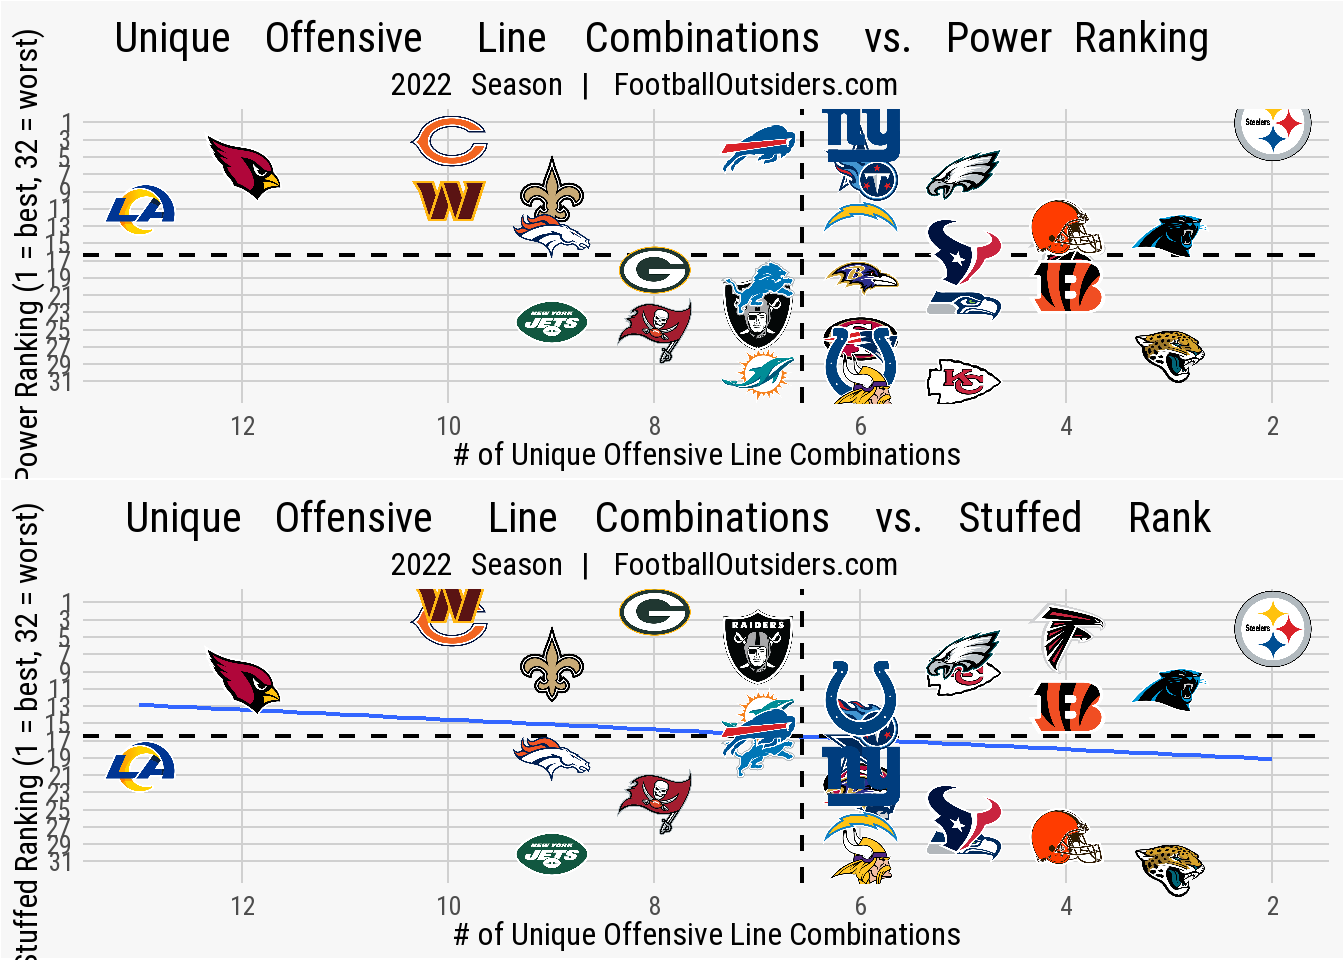
\includegraphics{01-nfl-analytics-and-r_files/figure-pdf/power-and-stuff-cowplot-1.pdf}

}

\end{figure}

Based on the results, it does not seem that the number of unique
offensive line combinations has impact on either power rank or stuffed
rank. The Los Angeles Rams and Arizona Cardinals, despite have the two
highest unique line combinations, are among the best in the league in
the metric. In fact, the opposite seems to be true in that the Minnesota
Vikings, with just six unique line combinations during the 2022 season,
are last in the league in power ranking. The Rams performed in bit worse
when comparing line combinations to stuffed rank, but the Cardinals are
still among the best in the league. The Vikings again are at the bottom,
only under performed by the Jacksonville Jaguars (who had just three
unique combinations throughout the season).

\begin{Shaded}
\begin{Highlighting}[]
\FunctionTok{ggplot}\NormalTok{(fb\_outsiders\_oline, }\FunctionTok{aes}\NormalTok{(}\AttributeTok{x =}\NormalTok{ combos, }\AttributeTok{y =}\NormalTok{ adj\_line\_yards)) }\SpecialCharTok{+}
  \FunctionTok{geom\_smooth}\NormalTok{(}\AttributeTok{method =} \StringTok{"lm"}\NormalTok{, }\AttributeTok{se =} \ConstantTok{FALSE}\NormalTok{, }\AttributeTok{size =} \FloatTok{0.8}\NormalTok{, }\AttributeTok{alpha =}\NormalTok{ .}\DecValTok{08}\NormalTok{) }\SpecialCharTok{+}
\NormalTok{  nflplotR}\SpecialCharTok{::}\FunctionTok{geom\_mean\_lines}\NormalTok{(}\FunctionTok{aes}\NormalTok{(}\AttributeTok{v\_var =}\NormalTok{ combos, }\AttributeTok{h\_var =}\NormalTok{ adj\_line\_yards),}
                            \AttributeTok{color =} \StringTok{"black"}\NormalTok{, }\AttributeTok{size =}\NormalTok{ .}\DecValTok{8}\NormalTok{) }\SpecialCharTok{+}
\NormalTok{  nflplotR}\SpecialCharTok{::}\FunctionTok{geom\_nfl\_logos}\NormalTok{(}\FunctionTok{aes}\NormalTok{(}\AttributeTok{team\_abbr =}\NormalTok{ team), }\AttributeTok{width =} \FloatTok{0.065}\NormalTok{) }\SpecialCharTok{+}
  \FunctionTok{scale\_x\_reverse}\NormalTok{(}\AttributeTok{breaks =}\NormalTok{ scales}\SpecialCharTok{::}\FunctionTok{pretty\_breaks}\NormalTok{()) }\SpecialCharTok{+}
  \FunctionTok{scale\_y\_continuous}\NormalTok{(}\AttributeTok{breaks =}\NormalTok{ scales}\SpecialCharTok{::}\FunctionTok{pretty\_breaks}\NormalTok{()) }\SpecialCharTok{+}
  \FunctionTok{labs}\NormalTok{(}\AttributeTok{title =} \StringTok{"**Unique Offensive Line Combinations vs. Adjusted Line Yards**"}\NormalTok{,}
       \AttributeTok{subtitle =} \StringTok{"*2022 Season  |  FootballOutsiders.com*"}\NormalTok{,}
       \AttributeTok{caption =} \StringTok{"*An Introduction to NFL Analytics with R*\textless{}br\textgreater{}**Brad J. Congelio**"}\NormalTok{) }\SpecialCharTok{+}
  \FunctionTok{xlab}\NormalTok{(}\StringTok{"\# of Unique Offensive Line Combinations"}\NormalTok{) }\SpecialCharTok{+}
  \FunctionTok{ylab}\NormalTok{(}\StringTok{"Adjusted Line Yards"}\NormalTok{) }\SpecialCharTok{+}
  \FunctionTok{nfl\_analytics\_theme}\NormalTok{()}
\end{Highlighting}
\end{Shaded}

\begin{verbatim}
`geom_smooth()` using formula = 'y ~ x'
\end{verbatim}

\begin{figure}[H]

{\centering 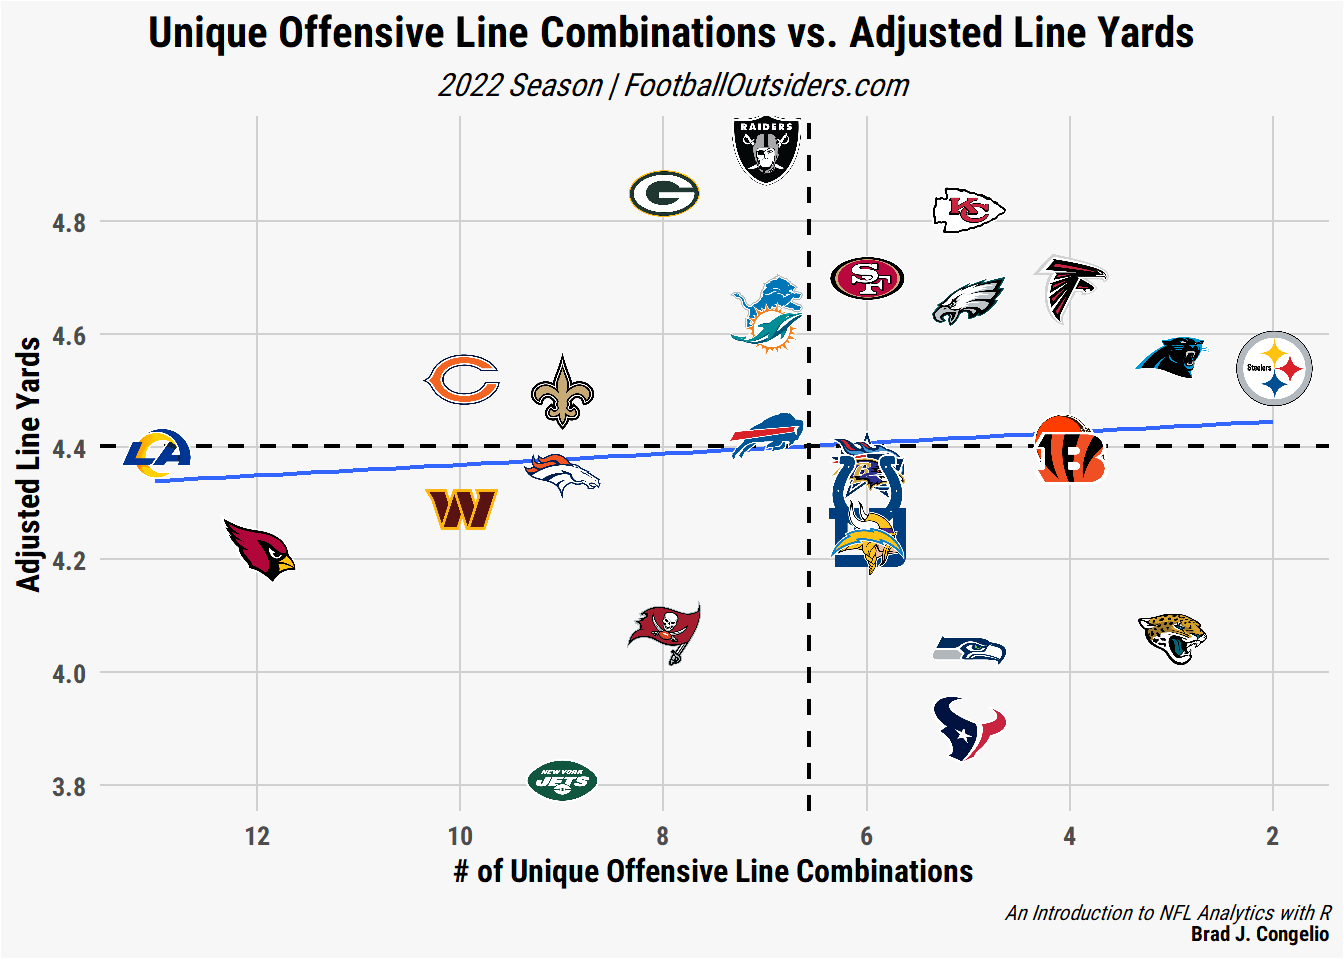
\includegraphics{01-nfl-analytics-and-r_files/figure-pdf/adj-yard-line-plot-1.pdf}

}

\end{figure}

Comparing a team's unique offensive line combinations to adjusted line
yards is more promising than power and stuffed rank, as the team's with
the highest amount of combinations begin to fall under the
league-average line for ALY. There are still several teams that, despite
having a low number of combinations through the season, performed poorly
such as the Houston Texans, Seattle Seahawks, and the Jaguars.

So what do we make of this?

Given that adjusted line yards is constructed to measure the
responsibility of the offensive line, it is logical to also want to
consider the ``performance'' of the running back. A running back that is
able to avoid early hits, or break tackles and earn yards after contact,
can overcome an under performing offensive line (whether that be from
lack of talent or lack of cohesiveness from a high number of
combinations). In the description of the adjusted line yards metrics,
Football Outsiders confirms this, writing that a ``team with a very good
running back will appear higher no matter how bad their line, and a team
with a great line will appear lower if the running back is terrible.''

For the last exploration in this topic, we can bring in
\texttt{Elusive\ Rating}, which is a signature statistic from Pro
Football Focus that quantifies the ``success and impact of a runner with
the ball independently of the blocking. Let's bring in the data that
contains all of the information from \texttt{fb\_outsiders\_oline}, but
with the addition of an averaged \texttt{elusive} rating for each team
from PFF.

\begin{Shaded}
\begin{Highlighting}[]
\NormalTok{oline\_combo\_elusive }\OtherTok{\textless{}{-}}
  \FunctionTok{vroom}\NormalTok{(}\StringTok{"https://raw.githubusercontent.com/bcongelio/nfl{-}analytics{-}with{-}r{-}book/origin/example\_data/csv/online\_combo\_elusive.csv"}\NormalTok{)}
\end{Highlighting}
\end{Shaded}

Because we want to determine if the elusiveness of a team's stable of
running backs directly impacts the offensive line's Adjusted Line Yards,
we can create a new variable that use the team's
\texttt{elusive\_rating} to, in an elementary fashion, add weight to the
\texttt{adj\_line\_yards}. While there are numerous approaches to doing
so (such as ranking, categorical weighting, logarithmic weighting, using
coefficients from a regression model, etc.), we will conduct a more
simple type of feature engineering by first using the \texttt{scale()}
package to standardize the values, resulting in each team receiving what
is called a `z-score' (or the total standard deviations away from the
mean). After, we will created the \texttt{weighted\_aly} metric by
subtracting each team's z-score from the existing
\texttt{adj\_line\_yards}, and then plot the results.

\begin{Shaded}
\begin{Highlighting}[]
\NormalTok{oline\_combo\_elusive }\OtherTok{\textless{}{-}}\NormalTok{ oline\_combo\_elusive }\SpecialCharTok{\%\textgreater{}\%}
  \FunctionTok{mutate}\NormalTok{(}\AttributeTok{adjusted\_elu =} \FunctionTok{scale}\NormalTok{(avg\_elu),}
         \AttributeTok{weighted\_aly =}\NormalTok{ adj\_line\_yards }\SpecialCharTok{{-}}\NormalTok{ adjusted\_elu)}

\NormalTok{online\_combo\_test }\OtherTok{\textless{}{-}}\NormalTok{ oline\_combo\_elusive }\SpecialCharTok{\%\textgreater{}\%}
  \FunctionTok{mutate}\NormalTok{(}\AttributeTok{weighted\_aly =}\NormalTok{ adj\_line\_yards }\SpecialCharTok{{-}}\NormalTok{ adjusted\_elu)}

\FunctionTok{ggplot}\NormalTok{(oline\_combo\_elusive, }\FunctionTok{aes}\NormalTok{(}\AttributeTok{x =}\NormalTok{ combos, }\AttributeTok{y =}\NormalTok{ weighted\_aly)) }\SpecialCharTok{+}
  \FunctionTok{geom\_smooth}\NormalTok{(}\AttributeTok{method =} \StringTok{"lm"}\NormalTok{, }\AttributeTok{se =} \ConstantTok{FALSE}\NormalTok{, }\AttributeTok{size =} \FloatTok{0.8}\NormalTok{, }\AttributeTok{alpha =}\NormalTok{ .}\DecValTok{08}\NormalTok{) }\SpecialCharTok{+}
\NormalTok{  nflplotR}\SpecialCharTok{::}\FunctionTok{geom\_mean\_lines}\NormalTok{(}\FunctionTok{aes}\NormalTok{(}\AttributeTok{v\_var =}\NormalTok{ combos, }\AttributeTok{h\_var =}\NormalTok{ weighted\_aly),}
                            \AttributeTok{color =} \StringTok{"black"}\NormalTok{, }\AttributeTok{size =}\NormalTok{ .}\DecValTok{8}\NormalTok{) }\SpecialCharTok{+}
\NormalTok{  nflplotR}\SpecialCharTok{::}\FunctionTok{geom\_nfl\_logos}\NormalTok{(}\FunctionTok{aes}\NormalTok{(}\AttributeTok{team\_abbr =}\NormalTok{ team), }\AttributeTok{width =} \FloatTok{0.065}\NormalTok{) }\SpecialCharTok{+}
  \FunctionTok{scale\_x\_reverse}\NormalTok{(}\AttributeTok{breaks =}\NormalTok{ scales}\SpecialCharTok{::}\FunctionTok{pretty\_breaks}\NormalTok{()) }\SpecialCharTok{+}
  \FunctionTok{scale\_y\_continuous}\NormalTok{(}\AttributeTok{breaks =}\NormalTok{ scales}\SpecialCharTok{::}\FunctionTok{pretty\_breaks}\NormalTok{()) }\SpecialCharTok{+}
  \FunctionTok{labs}\NormalTok{(}\AttributeTok{title =} \StringTok{"**Unique Offensive Line Combinations vs. Weighted Adjusted Line Yards**"}\NormalTok{,}
       \AttributeTok{subtitle =} \StringTok{"*2022 Season  |  Adjusted with PFF\textquotesingle{}s \textquotesingle{}Elusive\textquotesingle{}*"}\NormalTok{,}
       \AttributeTok{caption =} \StringTok{"*An Introduction to NFL Analytics with R*\textless{}br\textgreater{}**Brad J. Congelio**"}\NormalTok{)}\SpecialCharTok{+}
  \FunctionTok{xlab}\NormalTok{(}\StringTok{"\# of Unique Offensive Line Combinations"}\NormalTok{) }\SpecialCharTok{+}
  \FunctionTok{ylab}\NormalTok{(}\StringTok{"Weighted Adjusted Line Yards"}\NormalTok{) }\SpecialCharTok{+}
  \FunctionTok{nfl\_analytics\_theme}\NormalTok{()}
\end{Highlighting}
\end{Shaded}

\begin{verbatim}
`geom_smooth()` using formula = 'y ~ x'
\end{verbatim}

\begin{figure}[H]

{\centering 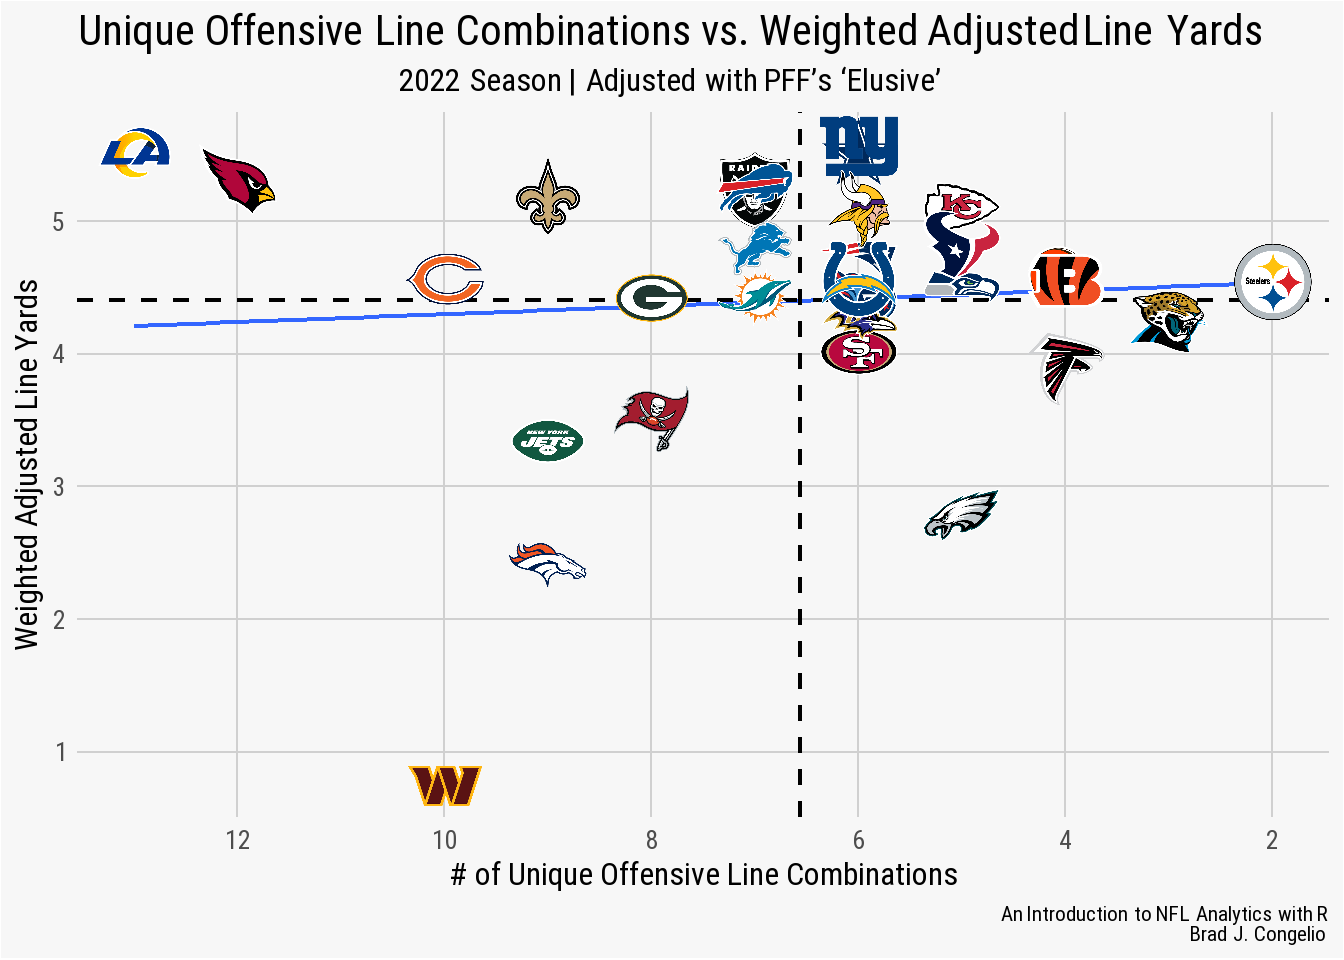
\includegraphics{01-nfl-analytics-and-r_files/figure-pdf/plotting-weighted-elusive-1.pdf}

}

\end{figure}

Despite having two of the bottom four scores in \texttt{elusive\_rating}
(21.4 and 21.8), the Rams and the Cardinals are in the league's top five
for \texttt{Weighted\ Adjusted\ Line\ Yard}. This is an indication that
each team's offensive line is proficient at run blocking and that any
perceived shortcoming in the ground game was the result of a lack of
elusive running backs. Conversely, the Washington Commanders unweighted
\texttt{Adjusted\ Line\ Yards} was 4.29 but, when account for the high
elusiveness score among the team's running backs, the metric dipped to a
league-worst 2.14 weighted adjusted line yards.

While there is certainly more examination that could be conducted, these
preliminary results seem to indicate that a higher number of unique
offensive line combinations has little impact on both the passing and
rushing games, with the exception of a general relationship with the
number of combinations and a team's adjusted sack rate. Even then, there
are caveats within the data that force us to consider further ways to
contextualize the data such as a quarterback's average time to release.

\hypertarget{exploring-explosive-plays-per-touchdown-drive}{%
\section{Exploring Explosive Plays per Touchdown
Drive}\label{exploring-explosive-plays-per-touchdown-drive}}

In November of 2022, Warren Sharp - of
\href{https://www.sharpfootballanalysis.com/}{Sharp Football Analysis} -
tweeted perhaps the most ridiculous statistic of the 2022 NFL season.

Heading into their week 9 bye week, the Steelers' longest play resulting
in a touchdown was just eight yards, or less than what is required for a
1st down. Perhaps making it worse, the touchdown came early in the
season, on a pass from Mitch Trubisky to Pat Freiermuth in a week 2
contest against the New England Patriots.

However, the statistics as presented by Sharp do not tell the complete
story as it isolates the entirety of a touchdown drive to a single play.
While the team's longest touchdown scoring play was just eight yards,
this does not mean that there was a lack of explosive, high-yardage
plays earlier in the drive that helped the Steelers get closer to the
endzone.

To determine if this is the case, we can construct a metric that explore
explosive plays per touchdown drive during the 2022 season.

\begin{Shaded}
\begin{Highlighting}[]
\NormalTok{pbp }\OtherTok{\textless{}{-}}\NormalTok{ nflreadr}\SpecialCharTok{::}\FunctionTok{load\_pbp}\NormalTok{(}\DecValTok{2022}\NormalTok{)}

\NormalTok{explosive }\OtherTok{\textless{}{-}}\NormalTok{ pbp }\SpecialCharTok{\%\textgreater{}\%}
  \FunctionTok{filter}\NormalTok{(}\SpecialCharTok{!}\FunctionTok{is.na}\NormalTok{(posteam) }\SpecialCharTok{\&}
           \SpecialCharTok{!}\FunctionTok{is.na}\NormalTok{(yards\_gained)}
         \SpecialCharTok{\&}\NormalTok{ fixed\_drive\_result }\SpecialCharTok{==} \StringTok{"Touchdown"}\NormalTok{) }\SpecialCharTok{\%\textgreater{}\%}
  \FunctionTok{filter}\NormalTok{(special }\SpecialCharTok{==} \DecValTok{0} \SpecialCharTok{\&}\NormalTok{ fumble }\SpecialCharTok{==} \DecValTok{0} \SpecialCharTok{\&}\NormalTok{ interception }\SpecialCharTok{==} \DecValTok{0}\NormalTok{) }\SpecialCharTok{\%\textgreater{}\%}
  \FunctionTok{group\_by}\NormalTok{(posteam, game\_id, drive) }\SpecialCharTok{\%\textgreater{}\%}
  \FunctionTok{summarize}\NormalTok{(}\AttributeTok{max\_yards =} \FunctionTok{max}\NormalTok{(yards\_gained)) }\SpecialCharTok{\%\textgreater{}\%}
  \FunctionTok{mutate}\NormalTok{(}\AttributeTok{explosive\_play =} \FunctionTok{if\_else}\NormalTok{(max\_yards }\SpecialCharTok{\textgreater{}=} \DecValTok{20}\NormalTok{, }\DecValTok{1}\NormalTok{, }\DecValTok{0}\NormalTok{)) }\SpecialCharTok{\%\textgreater{}\%}
  \FunctionTok{ungroup}\NormalTok{() }\SpecialCharTok{\%\textgreater{}\%}
  \FunctionTok{group\_by}\NormalTok{(posteam) }\SpecialCharTok{\%\textgreater{}\%}
  \FunctionTok{summarize}\NormalTok{(}\AttributeTok{tds\_no\_explosive =} \FunctionTok{sum}\NormalTok{(explosive\_play }\SpecialCharTok{==} \DecValTok{0}\NormalTok{),}
            \AttributeTok{tds\_explosive =} \FunctionTok{sum}\NormalTok{(explosive\_play }\SpecialCharTok{==} \DecValTok{1}\NormalTok{),}
            \AttributeTok{total\_drives =} \FunctionTok{sum}\NormalTok{(tds\_no\_explosive }\SpecialCharTok{+}\NormalTok{ tds\_explosive),}
            \AttributeTok{percent\_no\_exp =}\NormalTok{ tds\_no\_explosive }\SpecialCharTok{/}\NormalTok{ total\_drives,}
            \AttributeTok{percent\_w\_exp =}\NormalTok{ tds\_explosive }\SpecialCharTok{/}\NormalTok{ total\_drives) }\SpecialCharTok{\%\textgreater{}\%}
  \FunctionTok{select}\NormalTok{(posteam, percent\_w\_exp, percent\_no\_exp)}
\end{Highlighting}
\end{Shaded}

After collecting the play-by-play information for the 2022 NFL season,
we use \texttt{filter()} to gather only those
\texttt{fixed\_drive\_result} rows that include \texttt{Touchdown} and
then remove any play that is a special teams play and includes a fumble
or interception. This is done as we only want those touchdowns scored by
the offense, not a fumble or interception return for a score. Because of
this, the results of total touchdowns is lower than the ``official''
number from Pro Football Reference, as the site's ``Touchdown Log''
includes this data.

We then use \texttt{group\_by()} on \texttt{posteam}, \texttt{game\_id},
and \texttt{drive} in order to create the column \texttt{max\_yards}
with \texttt{summarize()}. The resulting numeric value in
\texttt{max\_yards} represents the largest amount of yards gained on a
single play, per drive. The important \texttt{explosive\_play} metric is
returned, in a binary \texttt{1} or \texttt{0} format, based on whether
or not the \texttt{max\_yards} in each drive was greater than or equal
to 20 yards. With this calculation complete, we \texttt{ungroup()} the
data and then group it only by \texttt{posteam} to determine the
results. After finding the percent of drives with an explosive play and
those without, we can plot the results.

\begin{Shaded}
\begin{Highlighting}[]
\FunctionTok{ggplot}\NormalTok{(explosive, }\FunctionTok{aes}\NormalTok{(}\AttributeTok{y =} \FunctionTok{reorder}\NormalTok{(posteam, percent\_w\_exp),}
                      \AttributeTok{x =}\NormalTok{ percent\_w\_exp)) }\SpecialCharTok{+}
  \FunctionTok{geom\_col}\NormalTok{(}\FunctionTok{aes}\NormalTok{(}\AttributeTok{color =}\NormalTok{ posteam, }\AttributeTok{fill =}\NormalTok{ posteam), }\AttributeTok{width =} \FloatTok{0.5}\NormalTok{) }\SpecialCharTok{+}
\NormalTok{  nflplotR}\SpecialCharTok{::}\FunctionTok{scale\_color\_nfl}\NormalTok{(}\AttributeTok{type =} \StringTok{"secondary"}\NormalTok{) }\SpecialCharTok{+}
\NormalTok{  nflplotR}\SpecialCharTok{::}\FunctionTok{scale\_fill\_nfl}\NormalTok{(}\AttributeTok{alpha =} \FloatTok{0.5}\NormalTok{) }\SpecialCharTok{+}
  \FunctionTok{nfl\_analytics\_theme}\NormalTok{() }\SpecialCharTok{+}
  \FunctionTok{theme}\NormalTok{(}\AttributeTok{axis.text.y =} \FunctionTok{element\_nfl\_logo}\NormalTok{(}\AttributeTok{size =}\NormalTok{ .}\DecValTok{65}\NormalTok{)) }\SpecialCharTok{+}
  \FunctionTok{scale\_x\_continuous}\NormalTok{(}\AttributeTok{expand =} \FunctionTok{c}\NormalTok{(}\DecValTok{0}\NormalTok{,}\DecValTok{0}\NormalTok{),}
                     \AttributeTok{breaks =}\NormalTok{ scales}\SpecialCharTok{::}\FunctionTok{pretty\_breaks}\NormalTok{(}\AttributeTok{n =} \DecValTok{5}\NormalTok{),}
                     \AttributeTok{label =}\NormalTok{ scales}\SpecialCharTok{::}\FunctionTok{percent\_format}\NormalTok{()) }\SpecialCharTok{+}
  \FunctionTok{labs}\NormalTok{(}\AttributeTok{title =} \StringTok{"**Which Team Has The Highest \% of Explosive Plays per TD Drive?**"}\NormalTok{,}
       \AttributeTok{subtitle =} \StringTok{"*2022 Season*"}\NormalTok{,}
       \AttributeTok{caption =} \StringTok{"*An Introduction to NFL Analytics with R*\textless{}br\textgreater{}**Brad J. Congelio**"}\NormalTok{) }\SpecialCharTok{+}
  \FunctionTok{xlab}\NormalTok{(}\StringTok{"Percent of TD Drives with an Explosive Play (20+ Yards)"}\NormalTok{) }\SpecialCharTok{+}
  \FunctionTok{ylab}\NormalTok{(}\StringTok{""}\NormalTok{)}
\end{Highlighting}
\end{Shaded}

\begin{figure}[H]

{\centering 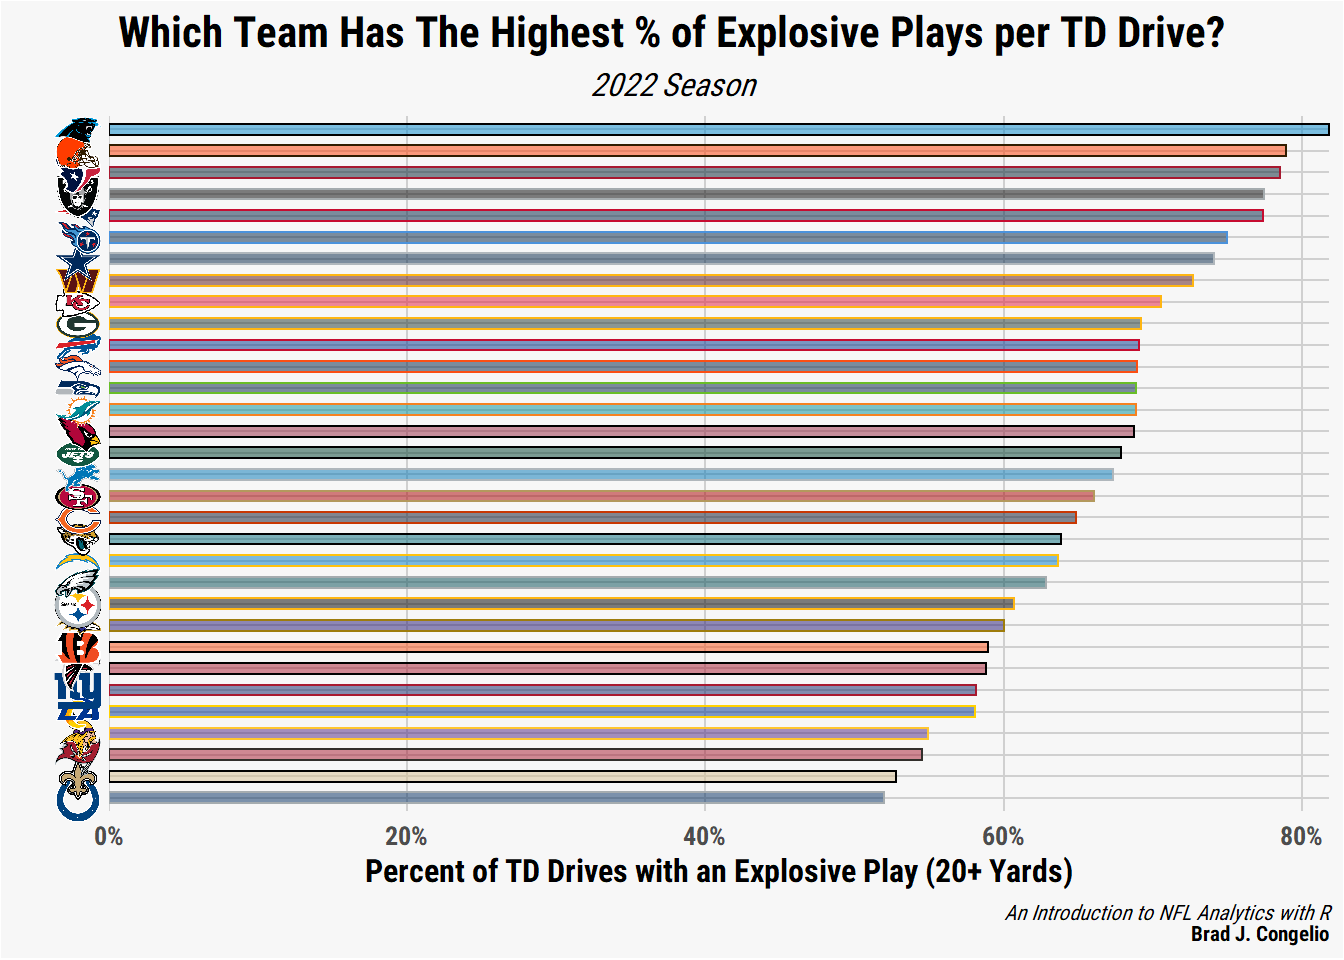
\includegraphics{01-nfl-analytics-and-r_files/figure-pdf/explosive-play-plot-1.pdf}

}

\end{figure}

The Carolina Panthers had a play that gained 20 or more yards on nearly
82\% of their touchdown drives, while the Indianapolis Colts had a
league-worst 52\% of touchdown drives including an explosive plays.
Notably, the Steelers are the near bottom as well with result of just
under 61\%. Given the statistic in Sharp's tweet, we can make an
assumption that Pittsburgh (as well as other the other teams with lower
percentages) methodically ``marched down'' the field on the way to
scoring touchdowns while teams such as the Panthers and Cleveland Browns
heavily relied on at least one big ``homerun'' play per touchdown drive
in order to move the ball

\bookmarksetup{startatroot}

\hypertarget{wrangling-nfl-data-in-the-tidyverse}{%
\chapter{\texorpdfstring{Wrangling NFL Data in the
\texttt{tidyverse}}{Wrangling NFL Data in the tidyverse}}\label{wrangling-nfl-data-in-the-tidyverse}}

\hypertarget{downloading-r-and-rstudio}{%
\section{Downloading R and RStudio}\label{downloading-r-and-rstudio}}

Prior to downloading R and RStudio, it is important to explain the
difference between the two, as they are separate pieces of our analytics
puzzle that are used for differing purposes. R is the core programming
language used for statistical computing and graphics. R provides a wide
range of statistical and graphical techniques and has a large community
of users who develop and maintain a multitude of packages (essentially
libraries of pre-written functions) that extend the capabilities and
ease of coding. While R can be run from your computer's command line, it
is also has an integrated development environment (IDE) in RStudio that
provides a graphical user interface for working with R scripts, data
files, and packages.

RStudio is free to download and use and provides a user-friendly
interface for writing R code, organizing projects and files, and working
with both big and small data. Regularly updated by the
\href{https://posit.co/}{Posit team}, RStudio includes many features
that are specifically designed to making working with R easier,
including syntax highlighting, code suggestions, robust debugging tools,
and a built-in package manager.

\begin{tcolorbox}[enhanced jigsaw, left=2mm, toprule=.15mm, opacitybacktitle=0.6, leftrule=.75mm, bottomrule=.15mm, colbacktitle=quarto-callout-important-color!10!white, breakable, colback=white, bottomtitle=1mm, toptitle=1mm, title=\textcolor{quarto-callout-important-color}{\faExclamation}\hspace{0.5em}{Important}, coltitle=black, titlerule=0mm, arc=.35mm, opacityback=0, colframe=quarto-callout-important-color-frame, rightrule=.15mm]

It is important that you download and successfully install R before
proceeding to install RStudio on your computer.

\end{tcolorbox}

\hypertarget{downloading-r}{%
\subsection{Downloading R}\label{downloading-r}}

\begin{enumerate}
\def\labelenumi{\arabic{enumi}.}
\tightlist
\item
  To download R, visit the official R website at
  \url{https://www.r-project.org/}
\item
  Click on the `CRAN' link at the top of the page, directly underneath
  the word `Download.' This will bring you to the Comprehensive R
  Archive Network.
\item
  Each mirror that hosts a copy of R is sorted by country. Select a
  mirror that is geographically close to you.
\item
  Click on the version of R that is appropriate for your operating
  system (Linux, macOS, or Windows).
\item
  Select the `base' option to download an updated version of R to your
  computer.
\item
  Open the downloaded file and follow the provided installation
  instructions.
\end{enumerate}

\hypertarget{downloading-rstudio}{%
\subsection{Downloading RStudio}\label{downloading-rstudio}}

\begin{enumerate}
\def\labelenumi{\arabic{enumi}.}
\tightlist
\item
  To download RStudio, visit the official RStudio website at
  \url{https://posit.co}
\item
  Click on the `Download RStudio' button in the top-right of the page.
\item
  Scroll down and select `Download' within the `RStudio Desktop - Free'
  box.
\item
  Open the downloaded file and follow the provided installation
  instructions.
\end{enumerate}

\hypertarget{the-layout-of-rstudio}{%
\subsection{The Layout of RStudio}\label{the-layout-of-rstudio}}

When you open RStudio for the first time, you will see the interface
laid out as in the picture below (sourced from the
\href{https://docs.posit.co/ide/user/ide/guide/ui/ui-panes.html}{official
RStudio documentation from posit}).

\begin{figure}

{\centering 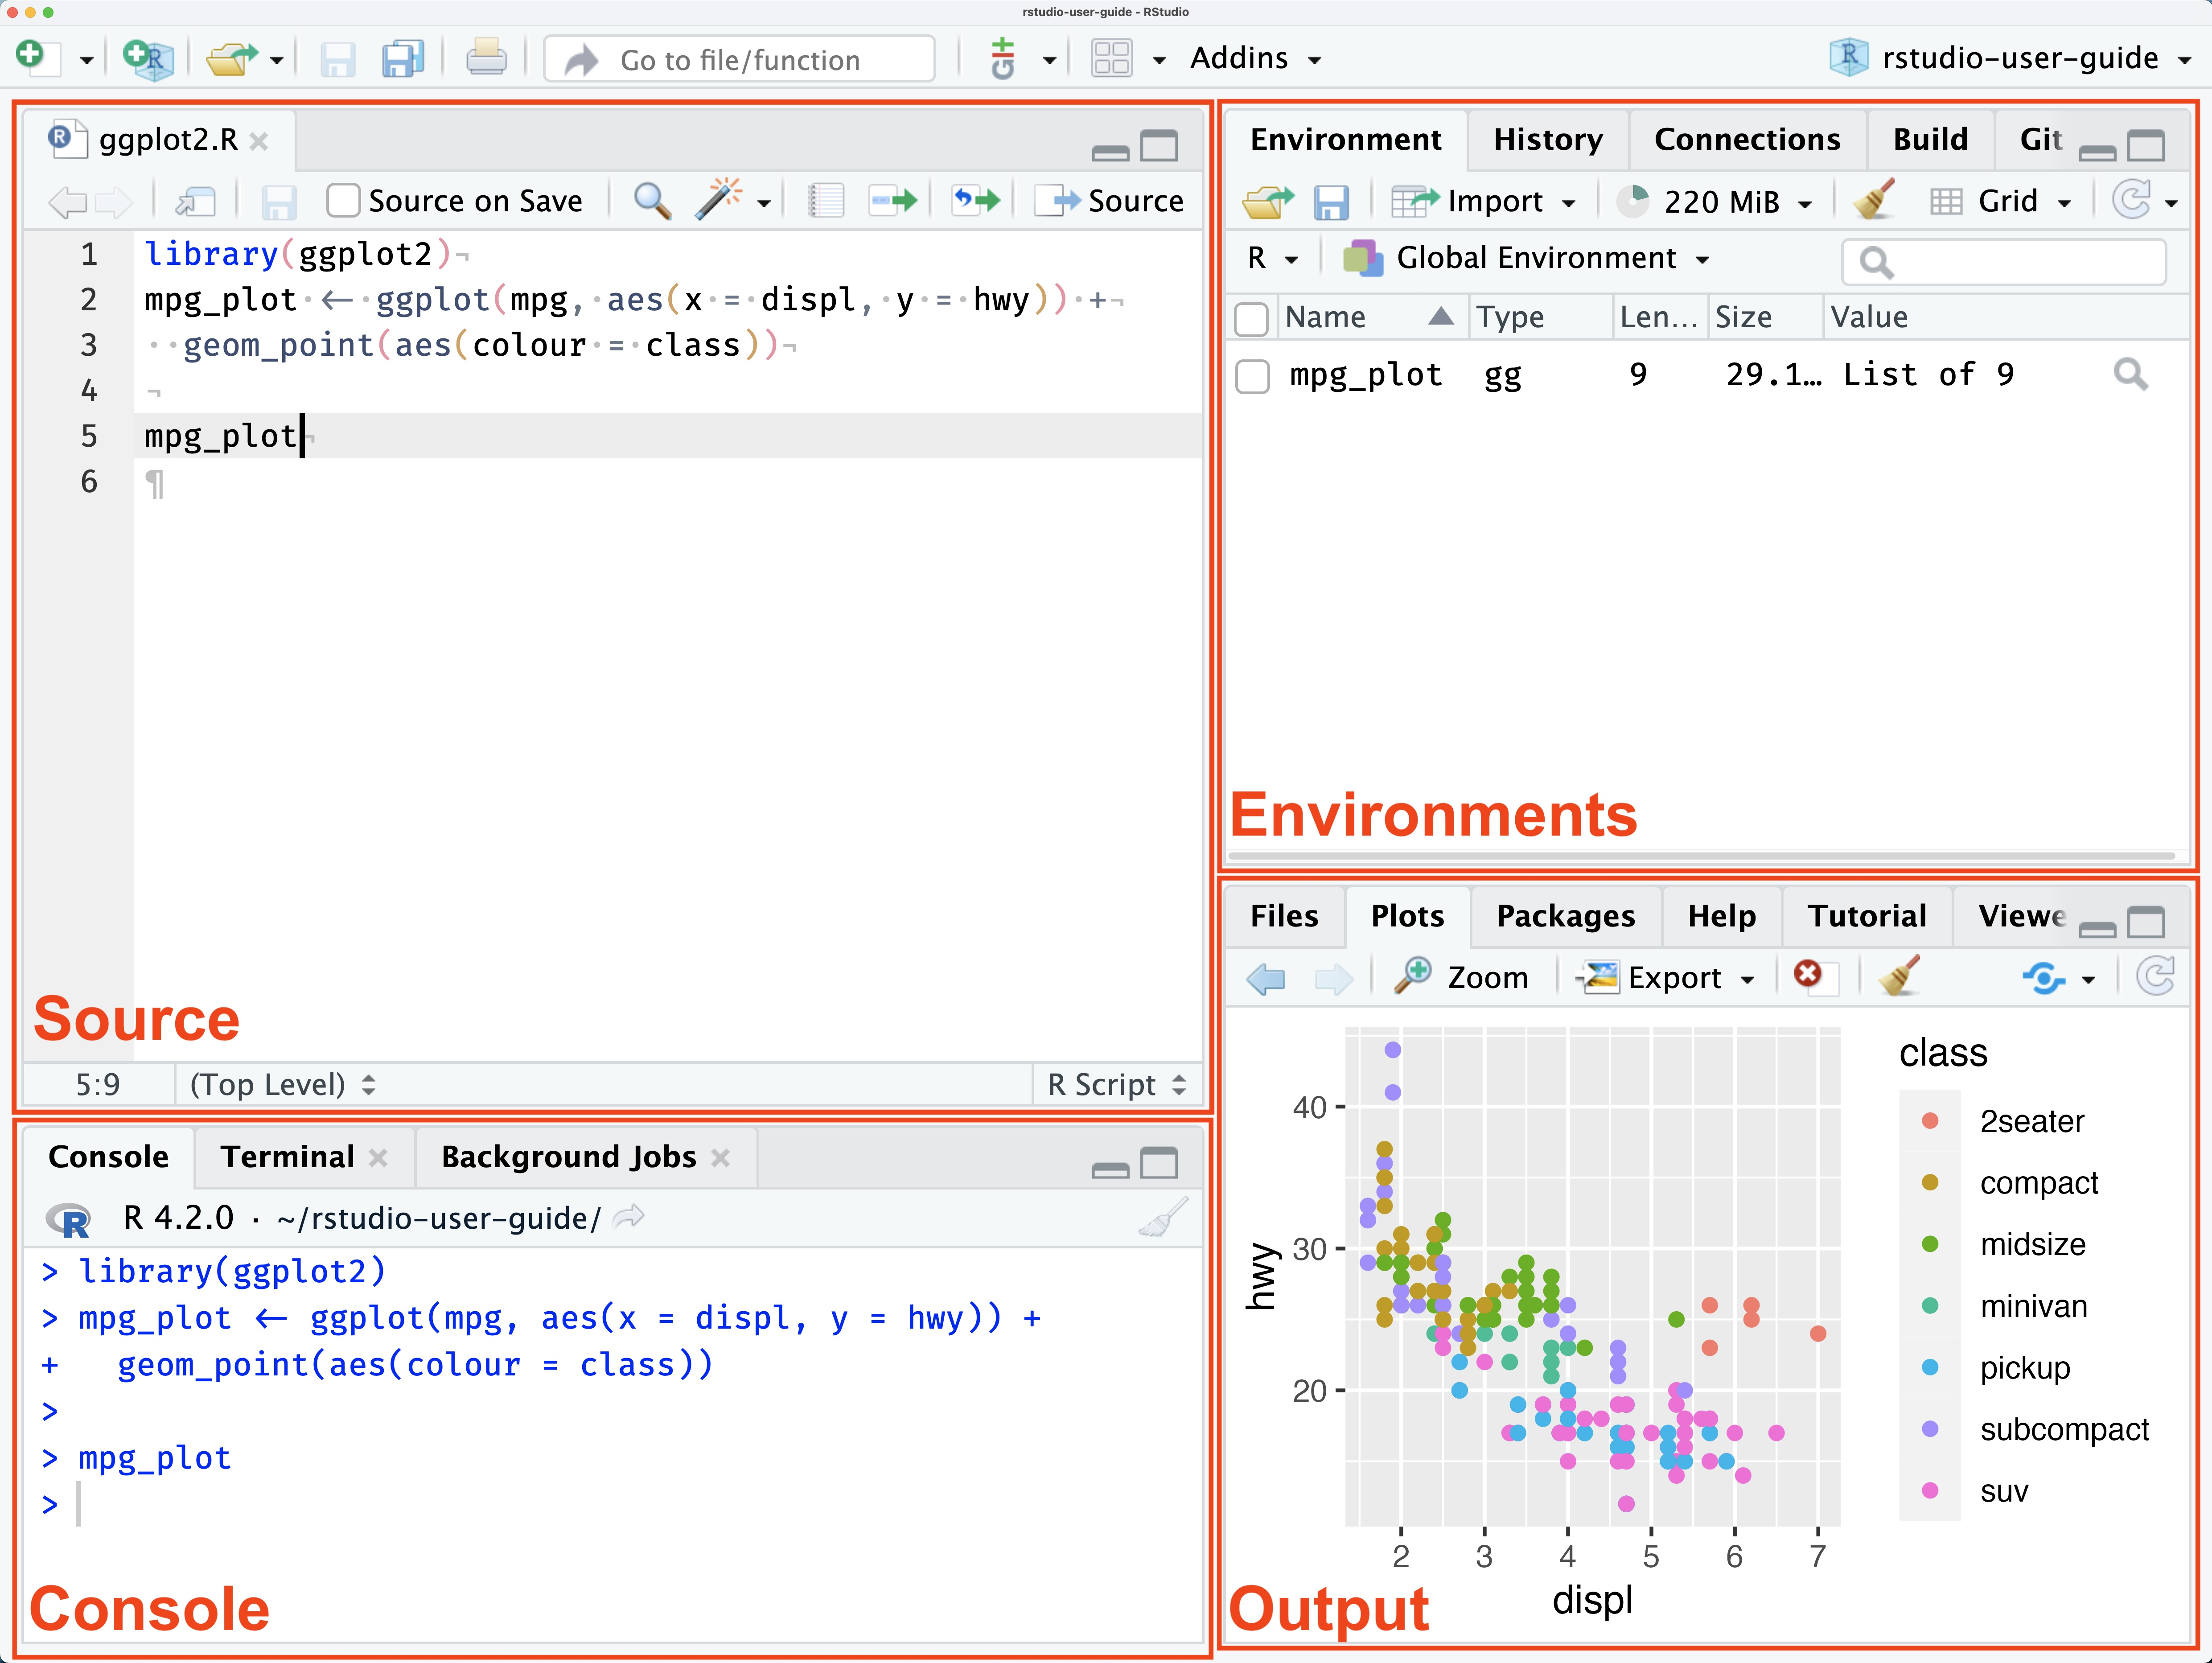
\includegraphics[width=4.58333in,height=\textheight]{images/rstudio-panes-with-labels.jpeg}

}

\end{figure}

As you can see, RStudio provides a graphical interface for working with
R and is sorted into four main panes, each of which serves a specific
purpose.

\begin{enumerate}
\def\labelenumi{\arabic{enumi}.}
\tightlist
\item
  \textbf{The source pane}: In the upper-left, the source pane is where
  you write and run your R code. It serves as the main working pane
  within RStudio.
\item
  \textbf{The console pane:} the console pane serves multiple functions,
  including allowing you to interact directly with R by typing commands
  and receiving the output. Additionally, any errors outputted by code
  ran in the source pane will be detailed in the console, allowing you
  to troubleshoot and debug.
\item
  \textbf{Environment and history pane}: this pane, in the upper-right,
  displays information about the current R environment and command
  history. Perhaps more important, it displays the information of all
  the R-created objects currently stored in your computer's memory
  including data sets, vectors, lists, etc.
\item
  \textbf{Files, plots, packages, and help pane}: in the bottom-right,
  this pane provides access to numerous RStudio tools and resources
  including the ability to browse and navigate through the files and
  folders on your computer and view the output of plots and graphics. As
  well, the `Packages' tab gives you the ability to manage any R
  packages that you have installed on your system and to view each
  packages' help documentation.
\end{enumerate}

\hypertarget{running-code-in-rstudio}{%
\subsection{Running Code in RStudio}\label{running-code-in-rstudio}}

To begin writing code in RStudio you first need to open a new R script.
To do so, select `File -\textgreater{} New File -\textgreater{} R
Script.' A new script tab, titled \texttt{Untitled\ 1} will open in your
RStudio's source pane. To run a line of code - or multiple lines of code
- you can do one of two options:

\begin{enumerate}
\def\labelenumi{\arabic{enumi}.}
\tightlist
\item
  Place your cursor directly at the end of the last line of code, or
  highlight all the code you wish to run, and press `Ctrl + Enter'
  (Windows) or `Command + Enter' (Mac).
\item
  Place your cursor directly at the end of the last line of code, or
  highlight all the code you wish to run, and then use your mouse to
  click the `Run' button in the source pane's toolbar.
\end{enumerate}

As a working example, let's do a simple addition problem within the the
source pane:

\begin{Shaded}
\begin{Highlighting}[]
\DecValTok{2} \SpecialCharTok{+} \DecValTok{2}
\end{Highlighting}
\end{Shaded}

After following one of the two above options for running the addition
problem, the output in your console should appear like below:

\begin{figure}

{\centering 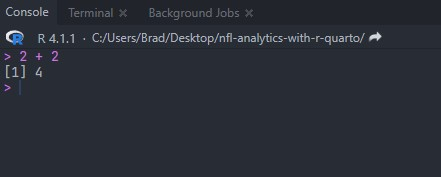
\includegraphics{images/example_console_output.jpg}

}

\end{figure}

\begin{tcolorbox}[enhanced jigsaw, left=2mm, toprule=.15mm, opacitybacktitle=0.6, leftrule=.75mm, bottomrule=.15mm, colbacktitle=quarto-callout-tip-color!10!white, breakable, colback=white, bottomtitle=1mm, toptitle=1mm, title=\textcolor{quarto-callout-tip-color}{\faLightbulb}\hspace{0.5em}{Tip}, coltitle=black, titlerule=0mm, arc=.35mm, opacityback=0, colframe=quarto-callout-tip-color-frame, rightrule=.15mm]

It is important to notice the \texttt{\textgreater{}} after the output
in the console. That indicates that the coding process has completely
run and RStudio is ready to run the next task that you submit. If you
have an error in your code, you will notice that the
\texttt{\textgreater{}} is replaced by what my students refer to as the
`hanging plus sign', \texttt{+}.

You receive the \texttt{+} sign when RStudio is expecting a continuation
of the code. Several issues can cause this to happen, including
forgetting to provide an equal number of opening and closing parenthesis
or mistakenly including a pipe, \texttt{\%\textgreater{}\%}, after the
last line of code.

In any case, when you see the \texttt{+} in the console, simply use your
mouse to click within the console and hit your keyboard's escape key.
Doing so exits the prompt and resets the console to include the
\texttt{\textgreater{}} symbol.

\end{tcolorbox}

\hypertarget{installing-and-loading-necessary-packages}{%
\section{Installing and Loading Necessary
Packages}\label{installing-and-loading-necessary-packages}}

Installing and loading packages is an important part of working with
RStudio, as they provide additional functionality that allow you to more
efficiently conduct data analysis and/or modeling. Several packages are
widely used through this book, including the ever-important
\texttt{tidyverse}, the \texttt{nflverse} family of packages to retrieve
NFL statistics and data, and many others such as \texttt{tidymodels}
when we tackle building and testing advanced models in Chapter 5.

To begin, let's install both \texttt{tidyverse} and \texttt{nflverse}.
In your source pane, you can install a package by using the
\texttt{install.packages()} function. To complete the code, you simply
supply the package name within quotation marks.

\begin{Shaded}
\begin{Highlighting}[]
\FunctionTok{install.packages}\NormalTok{(}\StringTok{"tidyverse"}\NormalTok{)}
\FunctionTok{install.packages}\NormalTok{(}\StringTok{"nflverse"}\NormalTok{)}
\end{Highlighting}
\end{Shaded}

After running the code, your console pane will output what is going on
``behind the scenes.'' When complete, you will again see the
\texttt{\textgreater{}} symbol within the console. At this point, you
are able to load the packages you just installed.

\begin{Shaded}
\begin{Highlighting}[]
\FunctionTok{library}\NormalTok{(tidyverse)}
\FunctionTok{library}\NormalTok{(nflverse)}
\end{Highlighting}
\end{Shaded}

\hypertarget{the-tidyverse-and-its-verbs}{%
\section{\texorpdfstring{The \texttt{tidyverse} and Its
Verbs}{The tidyverse and Its Verbs}}\label{the-tidyverse-and-its-verbs}}

The \texttt{tidyverse}, now installed and loaded within RStudio, is a
collection of R packages designed for data manipulation, visualization,
and analysis. It was developed by Hadley Wickham, the Chief Scientist at
Posit, and a varied team of contributors. The goal of the
\texttt{tidyverse} is to provide a consistent, easy-to-understand set of
functions and syntax for working with data in R.

The core principle of the \texttt{tidyverse} is ``tidy data,'' which is
the development team's belief in creating a standard way of organizing
data sets. To that end, a ``tidy'' data set is one that is comprised of
observations (rows) and variables (columns) with each variable being a
distinct piece of information and each observation being a unit of
analysis.

Installing and loading the \texttt{tidyverse} results eight of the core
packages automatically being loaded and ready to use:

\begin{enumerate}
\def\labelenumi{\arabic{enumi}.}
\tightlist
\item
  \textbf{dplyr:} ``dplyr provides a grammar of data manipulation,
  providing a consistent set of verbs that solve the most common data
  manipulation challenges.''
\item
  \textbf{tidyr:} ``tidyr provides a set of functions that help you get
  to tidy data. Tidy data is data with a consistent form: in brief,
  every variable goes in a column, and every column is a variable.''
\item
  \textbf{readr:} ``readr provides a fast and friendly way to read
  rectangular data (like csv, tsv, and fwf). It is deigned to flexibly
  parse many types of data found in the wild, while still cleanly
  failing when data unexpectedly changes.''
\item
  \textbf{purrr:} ``purrr enhances R's functional programming (FP)
  toolkit by providing a complete and consistent set of tools for
  working with functions and vectors. Once you master the basic
  concepts, purrr allows you to replace many for loops with code that is
  easier to write and more expressive.''
\item
  \textbf{tibble}: ``tibble is a modern re-imagining of the data frame,
  keeping what time has proven to be effective, and throwing out what it
  has not. Tibbles are data.frames that are lazy and surly; they do less
  and complain more forcing you to confront problems earlier, typically
  leading to cleaner, more expressive code.''
\item
  \textbf{stringr:} ``stringr provides a cohesive set of functions
  designed to make working with strings as easy as possible. It is built
  on top of stringi, which uses the ICU C library to provide fast,
  correct implementations of common string manipulations.''
\item
  \textbf{forcats:} ``forcats provides a suite of useful tools that
  solve common problems with factors. R uses factors to handle
  categorical variables, variables that have a fixed and known set of
  possible values.''
\item
  \textbf{ggplot2:} ``ggplot2 is a system for declaratively creating
  graphics, based on The Grammar of Graphics. You provide the data, tell
  ggplot2 how to map the variables to aesthetics, what graphical
  primitives to use, and it takes care of the details'' (Wickham 2022).
\end{enumerate}

Aside from the core eight packages, the \texttt{tidyverse} will also
install a multiple of other packages such as \texttt{rvest} (for web
scraping), \texttt{readxl} (for reading Excel sheets in the RStudio
environment), \texttt{lubridate} (a very powerful tool for working with
times and dates), and \texttt{magrittr} (the package that provides the
pipe \texttt{\%\textgreater{}\%}). As well, prior versions of the
\texttt{tidyverse} utilized the \texttt{modelr} package. Modeling is now
handled in the \texttt{tidyverse} by the \texttt{tidymodels} package.

\hypertarget{the-flow-of-the-tidyverse}{%
\section{\texorpdfstring{The Flow of the
\texttt{tidyverse}}{The Flow of the tidyverse}}\label{the-flow-of-the-tidyverse}}

The underlying design of coding in the \texttt{tidyverse}, aside from
the \texttt{dplyr} verbs, are both the assignment statement
(\texttt{\textless{}-}) and the pipe (\texttt{\%\textgreater{}\%}).
Please note, as mentioned in the book's Preface, that I still use the
pipe (\texttt{\%\textgreater{}\%}) that is part of the \texttt{magrittr}
package and not the native pipe operator
(\texttt{\textbar{}\textgreater{}}) included in the 4.1 release of R.
The choice of pipe operator you use is your decision to make, as either
will work seamlessly within the examples and activities provided in this
book.

As I explain to my Sports Analytics students, the language and flow of
the \texttt{tidyverse} can seem like a foreign language at first. But,
it is important that you stick with it because, sooner rather than
later, the light bulb above your head will go off. Before detailing the
in's and out's of the \texttt{tidyverse} in the below section, let's
first dissect an example of the \texttt{tidyverse} workflow.

\begin{Shaded}
\begin{Highlighting}[]
\NormalTok{pbp }\OtherTok{\textless{}{-}}\NormalTok{ nflreadr}\SpecialCharTok{::}\FunctionTok{load\_pbp}\NormalTok{(}\DecValTok{2022}\NormalTok{) }\SpecialCharTok{\%\textgreater{}\%}
  \FunctionTok{filter}\NormalTok{(posteam }\SpecialCharTok{==} \StringTok{"PHI"} \SpecialCharTok{\&}\NormalTok{ rush }\SpecialCharTok{==} \DecValTok{1}\NormalTok{) }\SpecialCharTok{\%\textgreater{}\%}
  \FunctionTok{group\_by}\NormalTok{(rusher) }\SpecialCharTok{\%\textgreater{}\%}
  \FunctionTok{summarize}\NormalTok{(}\AttributeTok{success\_rate =} \FunctionTok{mean}\NormalTok{(success))}
\end{Highlighting}
\end{Shaded}

The given example involves multiple iterations of the \texttt{tidyverse}
paradigm. At the outset of my Sport Analytics course, when introducing
the concepts of the \texttt{tidyverse}, I emphasize that it is possible
to ``talk your way through'' the process from the beginning to your end
goal (especially once you have you have a more comprehensive
understanding of the \texttt{dplyr} verbs, which are expounded upon in
the subsequent section). The following stepwise method illustrates this
using the above example of code:

\begin{enumerate}
\def\labelenumi{\arabic{enumi}.}
\tightlist
\item
  We first create a data set, denoted by \texttt{pbp}, by utilizing the
  \texttt{load\_pbp} function from the \texttt{nflreadr} package. To
  talk through this, you can say ``\texttt{pbp}is an copy of
  \texttt{nflreadr::load\_pbp(2022)}.'' While R purists may laugh at
  teaching the \texttt{tidyverse} in such language, it does indeed work.
  Going forward, the assignment operator (\texttt{\textless{}-}) simply
  implies that ``\emph{something is}.'' In this case, our \texttt{pbp}
  data frame \emph{is} the container for the play-by-play data we are
  collecting from \texttt{nflreadr}.
\item
  We then move into our first pipe operator
  (\texttt{\%\textgreater{}\%}). Again, R language purist will likely
  develop a eye twitch upon reading this, but I explain to my students
  that the pipe operator serves as a \emph{``\ldots{} and then''}
  command. In terms of the ``talk it out'' method above, the flow would
  be: ``\texttt{pbp} is a copy of \texttt{nflreadr::load\_pbp(2022)} and
  then \ldots{}''
\item
  After the pipe operator (or the first ``and then \ldots{}'' command),
  we move into our first \texttt{dplyr} verb. In this case, we are using
  the \texttt{filter} verb to select just the Philadelphia Eagles as the
  offensive team and just offensive plays that are rush attempts. With
  another pipe operator, we are including a second ``\emph{\ldots{} and
  then''} command.
\item
  To finish the example, we are grouping by each individual rusher on
  the Eagles ``\emph{and then''} summarize the average success rate for
  each rusher.
\end{enumerate}

\textbf{To put it together, ``talking it out'' from beginning to end
results in:}

``First, create a data set called \texttt{pbp} that is a copy of
\texttt{nflreadr::load\_pbp(2022)} \emph{and then} \texttt{filter} for
all instances where the \texttt{posteam} is \texttt{PHI} and
\texttt{rush\ ==\ 1} \emph{and then} \texttt{group\_by} each individual
rusher, \emph{and then} summarize the average success rate for each
rusher into a new column titled \texttt{success\_rate}.''

To showcase this visually, the ``talking through'' method is inputted
into the example code below:

\begin{Shaded}
\begin{Highlighting}[]
\NormalTok{pbp }\OtherTok{\textless{}{-}} \StringTok{"is"}\NormalTok{ nflreadr}\SpecialCharTok{::}\FunctionTok{load\_pbp}\NormalTok{(}\DecValTok{2022}\NormalTok{) }\SpecialCharTok{\%\textgreater{}\%} \StringTok{"... and then"}
  \FunctionTok{filter}\NormalTok{(posteam }\SpecialCharTok{==} \StringTok{"PHI"} \SpecialCharTok{\&}\NormalTok{ rush }\SpecialCharTok{==} \DecValTok{1}\NormalTok{) }\SpecialCharTok{\%\textgreater{}\%} \StringTok{"... and then"}
  \FunctionTok{group\_by}\NormalTok{(rusher) }\SpecialCharTok{\%\textgreater{}\%} \StringTok{"... and then"}
  \FunctionTok{summarize}\NormalTok{(}\AttributeTok{success\_rate =} \FunctionTok{mean}\NormalTok{(success))}
\end{Highlighting}
\end{Shaded}

\hypertarget{working-with-nfl-data-and-the-dplyr-verbs}{%
\section{\texorpdfstring{Working With NFL Data and the \texttt{dplyr}
Verbs}{Working With NFL Data and the dplyr Verbs}}\label{working-with-nfl-data-and-the-dplyr-verbs}}

Of the packages nestled within the \texttt{tidyverse}, \texttt{dplyr} is
perhaps the most important in terms of wrangling and cleaning data. As
mentioned above, \texttt{dplyr} is a powerful tool for data manipulation
in R as it provides a key set of functions, known as verbs, that are
designed to be easy to use and understand. The verbs can be used to
filter, group, summarize, rearrange, and transform all types of data
sets. For those just starting their NFL analytics endeavors in the R
programming language, the following four \texttt{dplyr} verbs are
perhaps the most important. Specific examples of working with these
verbs, as well as others, follow below.

\begin{enumerate}
\def\labelenumi{\arabic{enumi}.}
\tightlist
\item
  \texttt{filter}: the \texttt{filter()} verb allows you to subset data
  based on certain criteria. For example, you can use \texttt{filter()}
  to keep only those rows in a data set where a certain variable meets a
  certain conditions (ie., more than 100 completed passes). Moreover,
  the \texttt{filter()} verb can be used in conjunction with logical
  operators such as \texttt{\&} and \texttt{\textbar{}} to create more
  complex criteria.
\item
  \texttt{group\_by()}: the \texttt{group\_by()} verb allows you to
  group a data set by one or more variables. It is a useful tool when
  you want to perform an operation on each group, such as calculating a
  summary statistic (ie, intended air yards per quarterback) or when
  creating a plot.
\item
  \texttt{summarize()}: the \texttt{summarize()} verb allows you to
  reduce a data set to a single summary value. The \texttt{summarize()}
  verb is often used in conjunction with the \texttt{group\_by()}
  function, allowing you to group the data by one or more variables. The
  \texttt{summarize()} verb allows for a wide range of summary
  statistics, including means, medians, standard deviations, and more.
  You can also use it to calculate custom summary statistics.
\item
  \texttt{mutate()}: the \texttt{mutate()} verbs allows you to create
  new variables within your data while also preserving existing ones.
\end{enumerate}

\hypertarget{nfl-data-and-the-filter-verb}{%
\subsection{\texorpdfstring{NFL Data and the \texttt{filter()}
verb}{NFL Data and the filter() verb}}\label{nfl-data-and-the-filter-verb}}

The \texttt{filter()} verb allows you to extract specific rows from your
dataset based on one, or multiple, supplied conditions. The conditions
are supplied to the \texttt{filter()} verb by using logical operators,
listed in the below table, that ultimately evaluate to either
\texttt{TRUE} or \texttt{FALSE} in each row of the dataset. The
\texttt{filter()} process returns a data set that includes only those
rows that meet the specified conditions.

\begin{longtable}[]{@{}cc@{}}
\toprule\noalign{}
Logical Operator & Meaning \\
\midrule\noalign{}
\endhead
\bottomrule\noalign{}
\endlastfoot
\texttt{==} & equal to \\
\texttt{!=} & not equal to \\
\texttt{\textless{}} & less than \\
\texttt{\textless{}=} & less than or equal to \\
\texttt{\textgreater{}} & greater than \\
\texttt{\textgreater{}=} & greater than or equal to \\
\texttt{!} & not \\
\texttt{\&} & and \\
\texttt{\textbar{}} & or \\
\texttt{\%in\%} & includes \\
\texttt{c()} & used to combine arguments into a vector \\
\texttt{is.na} & checks for missing values \\
\texttt{!is.na} & is not missing specific values \\
\end{longtable}

In order to work through specific examples of the above logical
operators, we will use 2022 play-by-play data from \texttt{nflreadr}. To
begin, let's read in the data:

\begin{tcolorbox}[enhanced jigsaw, left=2mm, toprule=.15mm, opacitybacktitle=0.6, leftrule=.75mm, bottomrule=.15mm, colbacktitle=quarto-callout-note-color!10!white, breakable, colback=white, bottomtitle=1mm, toptitle=1mm, title=\textcolor{quarto-callout-note-color}{\faInfo}\hspace{0.5em}{Note}, coltitle=black, titlerule=0mm, arc=.35mm, opacityback=0, colframe=quarto-callout-note-color-frame, rightrule=.15mm]

Please note that a more detailed overview of reading in
\texttt{nflreadr} data is provided in Chapter 3. For the purposes of
learning about the \texttt{filter()} verb, please make sure you have
both the \texttt{tidyverse} and \texttt{nflreadr} loaded by running the
following:

\texttt{library(tidyverse})\\
\texttt{library(nflreadr)}

If you have difficult with the above step, please see the
\protect\hyperlink{installing-and-loading-necessary-packages}{Installing
and Loading Necessary Packages} section above.

\end{tcolorbox}

\begin{Shaded}
\begin{Highlighting}[]
\NormalTok{pbp }\OtherTok{\textless{}{-}}\NormalTok{ nflreadr}\SpecialCharTok{::}\FunctionTok{load\_pbp}\NormalTok{(}\DecValTok{2022}\NormalTok{)}
\end{Highlighting}
\end{Shaded}

After running the above code, you will have a data set titled
\texttt{pbp} placed into your RStudio environment consisting of 50,147
observations over 372 variables. With the data set loaded, let's create
a new data set titled \texttt{ne\_offense} that contains \emph{only
those plays where the New England Patriots are the offensive team}.

\begin{Shaded}
\begin{Highlighting}[]
\NormalTok{ne\_offense }\OtherTok{\textless{}{-}}\NormalTok{ pbp }\SpecialCharTok{\%\textgreater{}\%}
  \FunctionTok{filter}\NormalTok{(posteam }\SpecialCharTok{==} \StringTok{"NE"}\NormalTok{)}

\NormalTok{ne\_offense}
\end{Highlighting}
\end{Shaded}

\begin{verbatim}
-- nflverse play by play data --------------------------------------------------
\end{verbatim}

\begin{verbatim}
i Data updated: 2023-02-28 04:24:38 EST
\end{verbatim}

\begin{verbatim}
# A tibble: 1,323 x 372
   play_id game_id old_g~1 home_~2 away_~3 seaso~4  week posteam poste~5 defteam
     <dbl> <chr>   <chr>   <chr>   <chr>   <chr>   <int> <chr>   <chr>   <chr>  
 1      44 2022_0~ 202209~ MIA     NE      REG         1 NE      away    MIA    
 2      59 2022_0~ 202209~ MIA     NE      REG         1 NE      away    MIA    
 3      83 2022_0~ 202209~ MIA     NE      REG         1 NE      away    MIA    
 4     109 2022_0~ 202209~ MIA     NE      REG         1 NE      away    MIA    
 5     130 2022_0~ 202209~ MIA     NE      REG         1 NE      away    MIA    
 6     154 2022_0~ 202209~ MIA     NE      REG         1 NE      away    MIA    
 7     175 2022_0~ 202209~ MIA     NE      REG         1 NE      away    MIA    
 8     196 2022_0~ 202209~ MIA     NE      REG         1 NE      away    MIA    
 9     236 2022_0~ 202209~ MIA     NE      REG         1 NE      away    MIA    
10     571 2022_0~ 202209~ MIA     NE      REG         1 NE      away    MIA    
# ... with 1,313 more rows, 362 more variables: side_of_field <chr>,
#   yardline_100 <dbl>, game_date <chr>, quarter_seconds_remaining <dbl>,
#   half_seconds_remaining <dbl>, game_seconds_remaining <dbl>,
#   game_half <chr>, quarter_end <dbl>, drive <dbl>, sp <dbl>, qtr <dbl>,
#   down <dbl>, goal_to_go <dbl>, time <chr>, yrdln <chr>, ydstogo <dbl>,
#   ydsnet <dbl>, desc <chr>, play_type <chr>, yards_gained <dbl>,
#   shotgun <dbl>, no_huddle <dbl>, qb_dropback <dbl>, qb_kneel <dbl>, ...
\end{verbatim}

The output shows that the \texttt{posteam} variable contains only
\texttt{NE}, which is the abbreviation for the New England Patriots in
the \texttt{nflreadr} play-by-play data. In the code that produced
\texttt{ne\_offense}, \textbf{it is important to notice that:}

\begin{enumerate}
\def\labelenumi{\arabic{enumi}.}
\tightlist
\item
  the ``equal to'' logical operator consist of \emph{TWO} equal signs,
  not one.
\item
  the team abbreviation (\texttt{NE}) is in quotation marks.
\end{enumerate}

In the first, a single equal sign (\texttt{=}) can be used as a synonym
for assignment (\texttt{\textless{}-}) but is most often used when
passing values into functions. To avoid confusion with this possibility,
\textbf{the test for equality when using \texttt{filter()}} \textbf{is
always \texttt{==}}.

In the second, you must use quotation marks around the character-based
value you are placing into the \texttt{filter()} verb because, if not, R
will interpret \texttt{posteam} incorrectly and ultimately generate an
error. On the other hand, you \emph{do not}~need to include quotation
marks if you are filtering out numeric-based variables. Below are
incorrect and correct examples of both:

\begin{Shaded}
\begin{Highlighting}[]
\NormalTok{ne\_offense }\OtherTok{\textless{}{-}}\NormalTok{ pbp }\SpecialCharTok{\%\textgreater{}\%}
  \FunctionTok{filter}\NormalTok{(posteam }\SpecialCharTok{==}\NormalTok{ NE) }\CommentTok{\#this is incorrect.}
                        \DocumentationTok{\#\#Character values must be in quotation marks.}

\NormalTok{ne\_offense }\OtherTok{\textless{}{-}}\NormalTok{ pbp }\SpecialCharTok{\%\textgreater{}\%}
  \FunctionTok{filter}\NormalTok{(posteam }\SpecialCharTok{==} \StringTok{"NE"}\NormalTok{) }\CommentTok{\#this is correct for character values.}

\NormalTok{ne\_offense }\OtherTok{\textless{}{-}}\NormalTok{ pbp }\SpecialCharTok{\%\textgreater{}\%}
  \FunctionTok{filter}\NormalTok{(air\_yards }\SpecialCharTok{\textgreater{}=} \StringTok{"5"}\NormalTok{) }\CommentTok{\#this is incorrect.}
                           \CommentTok{\#Numeric values do not need quotation marks.}

\NormalTok{ne\_offense }\OtherTok{\textless{}{-}}\NormalTok{ pbp }\SpecialCharTok{\%\textgreater{}\%}
  \FunctionTok{filter}\NormalTok{(air\_yards }\SpecialCharTok{\textgreater{}=} \DecValTok{5}\NormalTok{) }\CommentTok{\#this is correct for numeric values.}
\end{Highlighting}
\end{Shaded}

How do we approach the logical operators if we want to retrieve every
offensive team in the \texttt{pbp} data \emph{except} for New England?
In that case, we can use the ``not equal to'' (\texttt{!=}) operator:

\begin{Shaded}
\begin{Highlighting}[]
\NormalTok{not\_ne\_offense }\OtherTok{\textless{}{-}}\NormalTok{ pbp }\SpecialCharTok{\%\textgreater{}\%}
  \FunctionTok{filter}\NormalTok{(posteam }\SpecialCharTok{!=} \StringTok{"NE"}\NormalTok{)}
\end{Highlighting}
\end{Shaded}

The resulting data set titled \texttt{not\_ne\_offense} will still
include all 372 variables housed within the \texttt{nflreadr}
play-by-play data, but will not include any row in which New England is
the offensive (\texttt{posteam}) team.

\textbf{Continuing with examples, how do we use the \texttt{filter()}}
\textbf{verb on multiple teams at once?} For instance, let's use the
above filtering process for offensive teams but only retrieve
information from the play-by-play data for the four teams that comprise
the AFC East (Buffalo Bills, Miami Dolphins, New England Patriots, and
the New York Jets). There are, in fact, two logical operators that can
produce the results we are looking for: the ``or'' logical operator
(\texttt{\textbar{}}) or by using the ``includes'' logical operator
(\texttt{\%in\%}) combined with the ``concatenate'' operator
(\texttt{c()}). Let's start with using the ``or'' operator.

\begin{Shaded}
\begin{Highlighting}[]
\NormalTok{afc\_east }\OtherTok{\textless{}{-}}\NormalTok{ pbp }\SpecialCharTok{\%\textgreater{}\%}
  \FunctionTok{filter}\NormalTok{(posteam }\SpecialCharTok{==} \StringTok{"NE"} \SpecialCharTok{|}\NormalTok{ posteam }\SpecialCharTok{==} \StringTok{"MIA"}
         \SpecialCharTok{|}\NormalTok{ posteam }\SpecialCharTok{==} \StringTok{"NYJ"} \SpecialCharTok{|}\NormalTok{ posteam }\SpecialCharTok{==} \StringTok{"BUF"}\NormalTok{)}
\end{Highlighting}
\end{Shaded}

By using the \texttt{\textbar{}} logical operator, which translates to
the word ``or'', we can string together for separate filters for
\texttt{posteam} within the play-by-platy data. That said, it probably
seems odd to have to include the \texttt{posteam} argument four
different times, rather than being able to do this:

\begin{Shaded}
\begin{Highlighting}[]
\NormalTok{afc\_east }\OtherTok{\textless{}{-}}\NormalTok{ pbp }\SpecialCharTok{\%\textgreater{}\%}
  \FunctionTok{filter}\NormalTok{(posteam }\SpecialCharTok{==} \StringTok{"NE"} \SpecialCharTok{|} \StringTok{"MIA"} \SpecialCharTok{|} \StringTok{"NYJ"} \SpecialCharTok{|} \StringTok{"BUF"}\NormalTok{)}
\end{Highlighting}
\end{Shaded}

While the above example logically makes sense (verbally saying
``\texttt{posteam} equals NE or MIA or NYJ or BUF''), it unfortunately
results in an error. To that end, if you'd rather avoid the need to type
\texttt{posteam} four different times, as in the above example, you can
switch to using the \texttt{\%in\%} operator combined with \texttt{c()}.
It is possible to combine just \texttt{filter()} and the \texttt{\%in\%}
operator to retrieve one specific team. But, as in the above example
where, we will receive an error if we try to do it for multiple teams
without including the \texttt{c()} operator, as such:

\begin{Shaded}
\begin{Highlighting}[]
\NormalTok{afc\_east }\OtherTok{\textless{}{-}}\NormalTok{ pbp }\SpecialCharTok{\%\textgreater{}\%}
  \FunctionTok{filter}\NormalTok{(posteam }\SpecialCharTok{\%in\%} \FunctionTok{c}\NormalTok{(}\StringTok{"NE"}\NormalTok{, }\StringTok{"MIA"}\NormalTok{, }\StringTok{"NYJ"}\NormalTok{, }\StringTok{"BUF"}\NormalTok{))}

\NormalTok{afc\_east}
\end{Highlighting}
\end{Shaded}

\begin{verbatim}
-- nflverse play by play data --------------------------------------------------
\end{verbatim}

\begin{verbatim}
i Data updated: 2023-02-28 04:24:38 EST
\end{verbatim}

\begin{verbatim}
# A tibble: 5,625 x 372
   play_id game_id old_g~1 home_~2 away_~3 seaso~4  week posteam poste~5 defteam
     <dbl> <chr>   <chr>   <chr>   <chr>   <chr>   <int> <chr>   <chr>   <chr>  
 1      43 2022_0~ 202209~ NYJ     BAL     REG         1 NYJ     home    BAL    
 2      68 2022_0~ 202209~ NYJ     BAL     REG         1 NYJ     home    BAL    
 3      89 2022_0~ 202209~ NYJ     BAL     REG         1 NYJ     home    BAL    
 4     115 2022_0~ 202209~ NYJ     BAL     REG         1 NYJ     home    BAL    
 5     136 2022_0~ 202209~ NYJ     BAL     REG         1 NYJ     home    BAL    
 6     172 2022_0~ 202209~ NYJ     BAL     REG         1 NYJ     home    BAL    
 7     391 2022_0~ 202209~ NYJ     BAL     REG         1 NYJ     home    BAL    
 8     412 2022_0~ 202209~ NYJ     BAL     REG         1 NYJ     home    BAL    
 9     436 2022_0~ 202209~ NYJ     BAL     REG         1 NYJ     home    BAL    
10     469 2022_0~ 202209~ NYJ     BAL     REG         1 NYJ     home    BAL    
# ... with 5,615 more rows, 362 more variables: side_of_field <chr>,
#   yardline_100 <dbl>, game_date <chr>, quarter_seconds_remaining <dbl>,
#   half_seconds_remaining <dbl>, game_seconds_remaining <dbl>,
#   game_half <chr>, quarter_end <dbl>, drive <dbl>, sp <dbl>, qtr <dbl>,
#   down <dbl>, goal_to_go <dbl>, time <chr>, yrdln <chr>, ydstogo <dbl>,
#   ydsnet <dbl>, desc <chr>, play_type <chr>, yards_gained <dbl>,
#   shotgun <dbl>, no_huddle <dbl>, qb_dropback <dbl>, qb_kneel <dbl>, ...
\end{verbatim}

The above approach is a simplified version of first creating a vector of
the team abbreviations and then passing that into the \texttt{filter()}
argument. For example, we can create the following vector that appears
in the ``Values'' area of your RStudio environment, and then use that to
retrieve the same results in did in the above code:

\begin{Shaded}
\begin{Highlighting}[]
\NormalTok{afc\_east\_teams\_vector }\OtherTok{\textless{}{-}} \FunctionTok{c}\NormalTok{(}\StringTok{"NE"}\NormalTok{, }\StringTok{"MIA"}\NormalTok{, }\StringTok{"NYJ"}\NormalTok{, }\StringTok{"BUF"}\NormalTok{)}

\NormalTok{afc\_east }\OtherTok{\textless{}{-}}\NormalTok{ pbp }\SpecialCharTok{\%\textgreater{}\%}
  \FunctionTok{filter}\NormalTok{(posteam }\SpecialCharTok{\%in\%}\NormalTok{ afc\_east\_teams\_vector)}

\NormalTok{afc\_east\_teams\_vector}
\end{Highlighting}
\end{Shaded}

\begin{verbatim}
[1] "NE"  "MIA" "NYJ" "BUF"
\end{verbatim}

In other cases, we may need to do the opposite of above - that is,
select all teams \emph{except} for specific ones. For example, using
data from \href{pff.com}{Pro Football Focus} regarding a quarterback's
average time to throw, let's determine how to \emph{remove} all AFC
North teams (Pittsburgh, Cleveland, Baltimore, and Cincinnati) from the
data set while leaving all other teams intact. Such a procedure is
necessary, for example, if we wanted to explore the average time to
throw for the combined AFC North teams against the rest of the NFL.

We cannot leave the data as is and find the averages outright. We must
remove the AFC North teams in order to avoid ``baking them into'' the
league-wide average, thus skewing the results of our analysis. To
complete this process, we turn to the \texttt{!} (``is not'') logical
operator.

To begin, we will use the \texttt{vroom} package to read in the data.

\begin{Shaded}
\begin{Highlighting}[]
\NormalTok{time\_in\_pocket }\OtherTok{\textless{}{-}}
  \FunctionTok{vroom}\NormalTok{(}\StringTok{"https://raw.githubusercontent.com/bcongelio/nfl{-}analytics{-}with{-}r{-}book/origin/example\_data/csv/time\_in\_pocket.csv"}\NormalTok{)}
\end{Highlighting}
\end{Shaded}

\begin{verbatim}
# A tibble: 30 x 5
   player          position team_name player_game_count avg_time_to_throw
   <chr>           <chr>    <chr>                 <dbl>             <dbl>
 1 Patrick Mahomes QB       KC                       20              2.85
 2 Tom Brady       QB       TB                       18              2.31
 3 Justin Herbert  QB       LAC                      18              2.75
 4 Joe Burrow      QB       CIN                      19              2.51
 5 Josh Allen      QB       BUF                      18              2.92
 6 Kirk Cousins    QB       MIN                      18              2.7 
 7 Trevor Lawrence QB       JAX                      19              2.51
 8 Geno Smith      QB       SEA                      18              2.79
 9 Daniel Jones    QB       NYG                      18              3.03
10 Jalen Hurts     QB       PHI                      18              2.86
# ... with 20 more rows
\end{verbatim}

The structure and organization of the data is quite similar to the data
sets we worked with in our above examples, despite coming from a
different source (PFF vs.~\texttt{nflreadr}). Our
\texttt{time\_in\_pocket} data includes a quarterback's name on each row
with his corresponding \texttt{team}, \texttt{player\_game\_count}, and
\texttt{avg\_time\_to\_throw}. Again, we are seeking to compare the
average time to release - combined - for the AFC North against the rest
of the NFL. In order to avoid skewing the results by ``baking in data''
(that is, not removing AFC North teams prior to finding the NFL
average), we can use the \texttt{!} logical operator to remove all four
teams at once (as oppose to structuring the \texttt{filter()} to include
four separate \texttt{team\_name\ !=} for all four different AFC North
teams.

\begin{Shaded}
\begin{Highlighting}[]
\NormalTok{time\_in\_pocket\_no\_afcn }\OtherTok{\textless{}{-}}\NormalTok{ time\_in\_pocket }\SpecialCharTok{\%\textgreater{}\%}
  \FunctionTok{filter}\NormalTok{(}\SpecialCharTok{!}\NormalTok{team\_name }\SpecialCharTok{\%in\%} \FunctionTok{c}\NormalTok{(}\StringTok{"PIT"}\NormalTok{, }\StringTok{"BAL"}\NormalTok{, }\StringTok{"CIN"}\NormalTok{, }\StringTok{"CLE"}\NormalTok{))}

\NormalTok{time\_in\_pocket\_no\_afcn}
\end{Highlighting}
\end{Shaded}

\begin{verbatim}
# A tibble: 26 x 5
   player          position team_name player_game_count avg_time_to_throw
   <chr>           <chr>    <chr>                 <dbl>             <dbl>
 1 Patrick Mahomes QB       KC                       20              2.85
 2 Tom Brady       QB       TB                       18              2.31
 3 Justin Herbert  QB       LAC                      18              2.75
 4 Josh Allen      QB       BUF                      18              2.92
 5 Kirk Cousins    QB       MIN                      18              2.7 
 6 Trevor Lawrence QB       JAX                      19              2.51
 7 Geno Smith      QB       SEA                      18              2.79
 8 Daniel Jones    QB       NYG                      18              3.03
 9 Jalen Hurts     QB       PHI                      18              2.86
10 Jared Goff      QB       DET                      17              2.7 
# ... with 16 more rows
\end{verbatim}

With Pittsburgh, Baltimore, Cincinnati, and Cleveland removed from the
data set, we can - for the sake of completing the analysis - take our
new \texttt{time\_in\_pocket\_afcn} data set and find the league-wide
average for \texttt{avg\_time\_to\_throw}.

\begin{Shaded}
\begin{Highlighting}[]
\NormalTok{time\_in\_pocket\_no\_afcn }\SpecialCharTok{\%\textgreater{}\%}
  \FunctionTok{summarize}\NormalTok{(}\AttributeTok{combined\_average =} \FunctionTok{mean}\NormalTok{(avg\_time\_to\_throw))}
\end{Highlighting}
\end{Shaded}

\begin{verbatim}
# A tibble: 1 x 1
  combined_average
             <dbl>
1             2.76
\end{verbatim}

\begin{Shaded}
\begin{Highlighting}[]
\NormalTok{time\_in\_pocket }\SpecialCharTok{\%\textgreater{}\%}
  \FunctionTok{filter}\NormalTok{(team\_name }\SpecialCharTok{\%in\%} \FunctionTok{c}\NormalTok{(}\StringTok{"PIT"}\NormalTok{, }\StringTok{"BAL"}\NormalTok{, }\StringTok{"CIN"}\NormalTok{, }\StringTok{"CLE"}\NormalTok{)) }\SpecialCharTok{\%\textgreater{}\%}
  \FunctionTok{summarize}\NormalTok{(}\AttributeTok{combined\_average =} \FunctionTok{mean}\NormalTok{(avg\_time\_to\_throw))}
\end{Highlighting}
\end{Shaded}

\begin{verbatim}
# A tibble: 1 x 1
  combined_average
             <dbl>
1             2.89
\end{verbatim}

The AFC North quarterbacks had an average time to throw of 2.76 seconds
while the rest of the NFL averaged 2.89 seconds, meaning the AFC North
QBs released the ball, on average, 0.13 seconds quicker than the rest of
the quarterbacks in the league.

So far, all our \texttt{filter()} operations have include just one
logical operator, or multiple values built into one operator using the
\texttt{\%in\%} option. However, because of the structure of the logical
operators, we are able to construct a single \texttt{filter()} combined
with various operator requests. For example, let's gather only those
rows that fit the following specifications:

\begin{enumerate}
\def\labelenumi{\arabic{enumi}.}
\tightlist
\item
  that play occurs on 2nd down.
\item
  the play must be a pass play.
\item
  the play must include a charted QB hit.
\item
  the play must result in a complete pass.
\item
  the pass must have an air yards amount that is greater than or equal
  to the yards to go.
\end{enumerate}

\begin{tcolorbox}[enhanced jigsaw, left=2mm, toprule=.15mm, opacitybacktitle=0.6, leftrule=.75mm, bottomrule=.15mm, colbacktitle=quarto-callout-tip-color!10!white, breakable, colback=white, bottomtitle=1mm, toptitle=1mm, title=\textcolor{quarto-callout-tip-color}{\faLightbulb}\hspace{0.5em}{Tip}, coltitle=black, titlerule=0mm, arc=.35mm, opacityback=0, colframe=quarto-callout-tip-color-frame, rightrule=.15mm]

Compiling the above \texttt{filter()} requires knowledge of the variable
names within \texttt{nflreadr} play-by-play data. This is covered in
Chapter 3.

That said, it is important to point out that many of the above variables
have data values that are structured in binary - that is, the value is
either 1 or 0.

In the above list, the \texttt{qb\_hit} variable is binary. A play
\emph{with} a QB hit is denoted by the inclusion of a numeric \texttt{1}
in the data, while the inclusion of a numeric \texttt{0} indicates that
a QB hit did not occur.

\end{tcolorbox}

Building the \texttt{filter()} based on the above specifications
requires the use of both character and numeric values:

\begin{Shaded}
\begin{Highlighting}[]
\NormalTok{multiple\_filters }\OtherTok{\textless{}{-}}\NormalTok{ pbp }\SpecialCharTok{\%\textgreater{}\%}
  \FunctionTok{filter}\NormalTok{(down }\SpecialCharTok{==} \DecValTok{2} \SpecialCharTok{\&}\NormalTok{ play\_type }\SpecialCharTok{==} \StringTok{"pass"} \SpecialCharTok{\&}
\NormalTok{           qb\_hit }\SpecialCharTok{==} \DecValTok{1} \SpecialCharTok{\&}
\NormalTok{           complete\_pass }\SpecialCharTok{==} \DecValTok{1} \SpecialCharTok{\&} 
\NormalTok{           air\_yards }\SpecialCharTok{\textgreater{}=}\NormalTok{ ydstogo)}
\end{Highlighting}
\end{Shaded}

The resulting data set, \texttt{multiple\_filters}, indicates that
exactly 105 such instances took place during the 2002 NFL season.

Lastly, in some instances, it is necessary to use \texttt{filter()} to
remove rows that may provide you with incorrect information if include.
To showcase this, it is necessary to also include the
\texttt{summarize()} verb, which is covered in greater detail in the
following two section. For example, let's gather information from the
play-by-play data that will provide the total amount of yards per
scrimmage - combined - for the 2022 regular season. Using our knowledge
from the prior example, we can write code that first uses the
\texttt{filter()} verb to retrieve just those rows that took place
during the regular season and then uses the \texttt{summarize()} verb to
distill the information down to the singular, combined total:

\begin{Shaded}
\begin{Highlighting}[]
\NormalTok{total\_yards }\OtherTok{\textless{}{-}}\NormalTok{ pbp }\SpecialCharTok{\%\textgreater{}\%}
  \FunctionTok{filter}\NormalTok{(season\_type }\SpecialCharTok{==} \StringTok{"REG"}\NormalTok{) }\SpecialCharTok{\%\textgreater{}\%}
  \FunctionTok{summarize}\NormalTok{(}\AttributeTok{yards =} \FunctionTok{sum}\NormalTok{(yards\_gained, }\AttributeTok{na.rm =} \ConstantTok{TRUE}\NormalTok{))}

\NormalTok{total\_yards}
\end{Highlighting}
\end{Shaded}

\begin{verbatim}
# A tibble: 1 x 1
   yards
   <dbl>
1 184444
\end{verbatim}

How many total scrimmage yards did NFL teams earn during the 2022 NFL
regular season? According to the results from our above code, the answer
is 184,444. However, that is incorrect.

The right answer, in fact, is 184,332 total scrimmage yards. How did the
results of our above coding come up 112 shorts of the correct answer (as
provided by the
\href{https://www.pro-football-reference.com/years/2022/\#all_team_stats}{2022
Team Stats page on Pro Football Reference})?

The difference is the result of the above code including all plays,
including 2-point conversion attempts. Because a 2-point conversion is
technically considered an extra point attempt - not a play from
scrimmage or an official down - no player stats are officially record
for the play. We can verify this is the case by using the
\texttt{filter()} verb to include only those rows that include
regular-season games and those plays that do not include information
pertaining to \texttt{down}:

\begin{Shaded}
\begin{Highlighting}[]
\NormalTok{two\_points }\OtherTok{\textless{}{-}}\NormalTok{ pbp }\SpecialCharTok{\%\textgreater{}\%}
  \FunctionTok{filter}\NormalTok{(season\_type }\SpecialCharTok{==} \StringTok{"REG"} \SpecialCharTok{\&} \FunctionTok{is.na}\NormalTok{(down)) }\SpecialCharTok{\%\textgreater{}\%}
  \FunctionTok{summarize}\NormalTok{(}\AttributeTok{total =} \FunctionTok{n}\NormalTok{(),}
            \AttributeTok{total\_yards =} \FunctionTok{sum}\NormalTok{(yards\_gained, }\AttributeTok{na.rm =} \ConstantTok{TRUE}\NormalTok{))}

\NormalTok{two\_points}
\end{Highlighting}
\end{Shaded}

\begin{verbatim}
# A tibble: 1 x 2
  total total_yards
  <int>       <dbl>
1  8137         112
\end{verbatim}

The results show that exactly 112 scrimmage yards were gained on places
missing \texttt{down} information. There was, of course, not 8,137
2-point conversion attempts during the 2022 regular season. There are
many other instances within the data that do not include information for
\texttt{down}, including: kickoffs, extra points, time outs, the end of
a quarter, etc. We can be more specific with our \texttt{filter()}
argument in the above code to include only the binary argument for the
\texttt{two\_point\_attempt} variable:

\begin{Shaded}
\begin{Highlighting}[]
\NormalTok{two\_points\_true }\OtherTok{\textless{}{-}}\NormalTok{ pbp }\SpecialCharTok{\%\textgreater{}\%}
  \FunctionTok{filter}\NormalTok{(season\_type }\SpecialCharTok{==} \StringTok{"REG"} \SpecialCharTok{\&}\NormalTok{ two\_point\_attempt }\SpecialCharTok{==} \DecValTok{1}\NormalTok{) }\SpecialCharTok{\%\textgreater{}\%}
  \FunctionTok{summarize}\NormalTok{(}\AttributeTok{total =} \FunctionTok{n}\NormalTok{(),}
            \AttributeTok{total\_yards =} \FunctionTok{sum}\NormalTok{(yards\_gained, }\AttributeTok{na.rm =} \ConstantTok{TRUE}\NormalTok{))}

\NormalTok{two\_points\_true}
\end{Highlighting}
\end{Shaded}

\begin{verbatim}
# A tibble: 1 x 2
  total total_yards
  <int>       <dbl>
1   119         112
\end{verbatim}

By altering the `\texttt{is.na(down)} argument to the binary indicator
for \texttt{two\_point\_attempt}, we see that there were 119 2-point
conversion attempts in the 2022 regular season while maintain the
correct 112 yards that explains our difference from above. To account
for our new-found knowledge that we must remove 2-point conversions to
calculate the correct amount of total scrimmage yards, we can again use
the \texttt{!is.na()} operator (where \texttt{!is.na()} means ``is not
missing this specific variable) to remove all rows that do not include
information pertaining to \texttt{down}:

\begin{Shaded}
\begin{Highlighting}[]
\NormalTok{total\_yards\_correct }\OtherTok{\textless{}{-}}\NormalTok{ pbp }\SpecialCharTok{\%\textgreater{}\%}
  \FunctionTok{filter}\NormalTok{(season\_type }\SpecialCharTok{==} \StringTok{"REG"} \SpecialCharTok{\&} \SpecialCharTok{!}\FunctionTok{is.na}\NormalTok{(down)) }\SpecialCharTok{\%\textgreater{}\%}
  \FunctionTok{summarize}\NormalTok{(}\AttributeTok{yards =} \FunctionTok{sum}\NormalTok{(yards\_gained, }\AttributeTok{na.rm =} \ConstantTok{TRUE}\NormalTok{))}

\NormalTok{total\_yards\_correct}
\end{Highlighting}
\end{Shaded}

\begin{verbatim}
# A tibble: 1 x 1
   yards
   <dbl>
1 184332
\end{verbatim}

By filtering out any row that does not include the \texttt{down} for a
given play, we correctly calculated the total amount of scrimmage yards
- 184,332 - for the 2022 NFL regular season.

\hypertarget{nfl-data-and-the-group_by-verb}{%
\subsection{\texorpdfstring{NFL Data and the \texttt{group\_by()}
verb}{NFL Data and the group\_by() verb}}\label{nfl-data-and-the-group_by-verb}}

As mentioned above, the \texttt{group\_by()} verb allows you to group
data by one or more specific variables in order to retrieve, among other
actions, summary statistics. To showcase how \texttt{group\_by()} is
used within the \texttt{nflverse} data, let's first gather the 2022
regular season statistics and then use the \texttt{summarize()} verb to
get the average success rate on rushing plays.

As well, we immediately make use of the \texttt{filter()} function to
sort the data : (1.) we first instruct to \texttt{filter()} the data to
include just those instances where the \texttt{play\_type} equals
\texttt{run}, (2.) we then say it must also be \texttt{play\ ==\ 1},
meaning there was no penalty or other interruption that ``cancelled
out'' the play, and (3.) we lastly pass the argument that the
\texttt{down} cannot be missing by using \texttt{!is.na} as a missing
down is indicative of a two-point conversion attempt.

\begin{Shaded}
\begin{Highlighting}[]
\NormalTok{rushing\_success\_ungrouped }\OtherTok{\textless{}{-}}\NormalTok{ pbp }\SpecialCharTok{\%\textgreater{}\%}
  \FunctionTok{filter}\NormalTok{(play\_type }\SpecialCharTok{==} \StringTok{"run"} \SpecialCharTok{\&}\NormalTok{ play }\SpecialCharTok{==} \DecValTok{1} \SpecialCharTok{\&} \SpecialCharTok{!}\FunctionTok{is.na}\NormalTok{(down)) }\SpecialCharTok{\%\textgreater{}\%}
  \FunctionTok{summarize}\NormalTok{(}\AttributeTok{success\_rate =} \FunctionTok{mean}\NormalTok{(success))}

\NormalTok{rushing\_success\_ungrouped}
\end{Highlighting}
\end{Shaded}

\begin{verbatim}
# A tibble: 1 x 1
  success_rate
         <dbl>
1        0.431
\end{verbatim}

Without including the \texttt{group\_by()} verb within the above code,
the output is the average success rate for rushing plays for all 32 NFL
teams, wherein success rate is the percentage of rushing plays that
resulted in an EPA above zero. In this case, approximately 43\% of NFL
rushes had a positive success rate.

That said, we are interested in examining the success rate by team, not
league-wide average. To do so, we add the \texttt{posteam} variable into
the \texttt{group\_by()} verb.

\begin{Shaded}
\begin{Highlighting}[]
\NormalTok{rushing\_success\_grouped }\OtherTok{\textless{}{-}}\NormalTok{ pbp }\SpecialCharTok{\%\textgreater{}\%}
  \FunctionTok{filter}\NormalTok{(play\_type }\SpecialCharTok{==} \StringTok{"run"} \SpecialCharTok{\&}\NormalTok{ play }\SpecialCharTok{==} \DecValTok{1} \SpecialCharTok{\&} \SpecialCharTok{!}\FunctionTok{is.na}\NormalTok{(down)) }\SpecialCharTok{\%\textgreater{}\%}
  \FunctionTok{group\_by}\NormalTok{(posteam) }\SpecialCharTok{\%\textgreater{}\%}
  \FunctionTok{summarize}\NormalTok{(}\AttributeTok{success\_rate =} \FunctionTok{mean}\NormalTok{(success)) }\SpecialCharTok{\%\textgreater{}\%}
  \FunctionTok{arrange}\NormalTok{(}\SpecialCharTok{{-}}\NormalTok{success\_rate)}

\NormalTok{rushing\_success\_grouped }\SpecialCharTok{\%\textgreater{}\%}
  \FunctionTok{slice}\NormalTok{(}\DecValTok{1}\SpecialCharTok{:}\DecValTok{10}\NormalTok{)}
\end{Highlighting}
\end{Shaded}

\begin{verbatim}
# A tibble: 10 x 2
   posteam success_rate
   <chr>          <dbl>
 1 PHI            0.526
 2 BUF            0.488
 3 BAL            0.478
 4 GB             0.476
 5 PIT            0.470
 6 ATL            0.463
 7 KC             0.459
 8 NYG            0.454
 9 CIN            0.454
10 LV             0.449
\end{verbatim}

In the above example, we have added the offensive team into the
\texttt{group\_by()} verb, while also arranging the data in descending
order by \texttt{success\_rate}, and then used \texttt{slice()} to
gather just the ten teams with the highest rushing success rate. The
Philadelphia Eagles led the NFL in rushing success rate during the 2022
NFL regular season at 52.3\%. By removing the \texttt{slice()} function
in the above example, we can see that Tampa Bay maintained the worst
rushing success rate in the league at 37.3\%.

While determining the rushing success rate of teams is interesting, we
can also determine the same metric for individual running backs as well.
To do so, we simply replace the variable in the \texttt{group\_by()}
verb. In the below example, we replace the \texttt{posteam} variable
with the \texttt{rusher} variable to see which running backs have the
highest success rate.

\begin{Shaded}
\begin{Highlighting}[]
\NormalTok{running\_back\_success }\OtherTok{\textless{}{-}}\NormalTok{ pbp }\SpecialCharTok{\%\textgreater{}\%}
  \FunctionTok{filter}\NormalTok{(play\_type }\SpecialCharTok{==} \StringTok{"run"} \SpecialCharTok{\&}\NormalTok{ play }\SpecialCharTok{==} \DecValTok{1} \SpecialCharTok{\&} \SpecialCharTok{!}\FunctionTok{is.na}\NormalTok{(down)) }\SpecialCharTok{\%\textgreater{}\%}
  \FunctionTok{group\_by}\NormalTok{(rusher) }\SpecialCharTok{\%\textgreater{}\%}
  \FunctionTok{summarize}\NormalTok{(}\AttributeTok{success\_rate =} \FunctionTok{mean}\NormalTok{(success)) }\SpecialCharTok{\%\textgreater{}\%}
  \FunctionTok{arrange}\NormalTok{(}\SpecialCharTok{{-}}\NormalTok{success\_rate)}

\NormalTok{running\_back\_success }\SpecialCharTok{\%\textgreater{}\%}
  \FunctionTok{slice}\NormalTok{(}\DecValTok{1}\SpecialCharTok{:}\DecValTok{10}\NormalTok{)}
\end{Highlighting}
\end{Shaded}

\begin{verbatim}
# A tibble: 10 x 2
   rusher      success_rate
   <chr>              <dbl>
 1 A.Davis                1
 2 B.Aiyuk                1
 3 B.Allen                1
 4 B.Skowronek            1
 5 C.Kmet                 1
 6 C.Sutton               1
 7 C.Wilson               1
 8 D.Bellinger            1
 9 D.Brown                1
10 D.Gray                 1
\end{verbatim}

The output, unfortunately, is not all that helpful. Because we did not
use the \texttt{filter()} verb to stipulate a minimum number of rushing
attempts, the output is saying that - for example, Daniel Bellinger, a
tight end, was among the most successful rushers in the league with a
100\% rushing success rate. To correct this, we must add a second metric
to our \texttt{summarize()} verb (we will call it \texttt{n\_rushes})
and then use the \texttt{filter()} verb afterwards to include a minimum
number of rushes required to be included in the final output.

As well, we will provide an additional argument in the first
\texttt{filter()} verb that stops the output from including any rushing
attempt that does not include the running back's name. The
\texttt{n\_rushes()} in the \texttt{summarize()} verb allows us to now
include the number of attempts, per individual rusher, that fall within
the first \texttt{filter()} parameter. Afterwards, we include a second
\texttt{filter()} argument to include just those rushers with at least
200 attempts.

\begin{Shaded}
\begin{Highlighting}[]
\NormalTok{running\_back\_success\_min }\OtherTok{\textless{}{-}}\NormalTok{ pbp }\SpecialCharTok{\%\textgreater{}\%}
  \FunctionTok{filter}\NormalTok{(play\_type }\SpecialCharTok{==} \StringTok{"run"} \SpecialCharTok{\&}\NormalTok{ play }\SpecialCharTok{==} \DecValTok{1} \SpecialCharTok{\&}
           \SpecialCharTok{!}\FunctionTok{is.na}\NormalTok{(down) }\SpecialCharTok{\&}
           \SpecialCharTok{!}\FunctionTok{is.na}\NormalTok{(rusher)) }\SpecialCharTok{\%\textgreater{}\%}
  \FunctionTok{group\_by}\NormalTok{(rusher) }\SpecialCharTok{\%\textgreater{}\%}
  \FunctionTok{summarize}\NormalTok{(}\AttributeTok{success\_rate =} \FunctionTok{mean}\NormalTok{(success),}
            \AttributeTok{n\_rushes =} \FunctionTok{n}\NormalTok{()) }\SpecialCharTok{\%\textgreater{}\%}
  \FunctionTok{filter}\NormalTok{(n\_rushes }\SpecialCharTok{\textgreater{}=} \DecValTok{200}\NormalTok{) }\SpecialCharTok{\%\textgreater{}\%}
  \FunctionTok{arrange}\NormalTok{(}\SpecialCharTok{{-}}\NormalTok{success\_rate)}

\NormalTok{running\_back\_success\_min }\SpecialCharTok{\%\textgreater{}\%}
  \FunctionTok{slice}\NormalTok{(}\DecValTok{1}\SpecialCharTok{:}\DecValTok{10}\NormalTok{)}
\end{Highlighting}
\end{Shaded}

\begin{verbatim}
# A tibble: 10 x 3
   rusher      success_rate n_rushes
   <chr>              <dbl>    <int>
 1 M.Sanders          0.483      294
 2 I.Pacheco          0.469      207
 3 A.Jones            0.465      213
 4 J.Jacobs           0.444      340
 5 N.Chubb            0.434      302
 6 T.Allgeier         0.429      210
 7 Ja.Williams        0.427      262
 8 T.Etienne          0.424      250
 9 J.Mixon            0.422      249
10 B.Robinson         0.420      205
\end{verbatim}

Unsurprisingly, Miles Sanders - a running back for the Eagles, who lead
the NFL in team success rate - is the leader in rushing success among
individual players with 49\% of his attempts gaining positive EPA.

Much like the \texttt{filter()} verb, we are able to supply multiple
arguments within one \texttt{group\_by()} verb. This is necessary, for
example, when you want to examine results over the course of multiple
seasons. Let's explore this by determining each team's yards after catch
between 2010 and 2022. To start, we will retrieve all NFL play-by-play
data from those seasons.

\begin{tcolorbox}[enhanced jigsaw, left=2mm, toprule=.15mm, opacitybacktitle=0.6, leftrule=.75mm, bottomrule=.15mm, colbacktitle=quarto-callout-caution-color!10!white, breakable, colback=white, bottomtitle=1mm, toptitle=1mm, title=\textcolor{quarto-callout-caution-color}{\faFire}\hspace{0.5em}{Caution}, coltitle=black, titlerule=0mm, arc=.35mm, opacityback=0, colframe=quarto-callout-caution-color-frame, rightrule=.15mm]

Loading in multiple seasons of play-by-play data can be taxing on your
computer's memory. RStudio's memory usage monitor, located in
`Environment' toolbar tell you how much data is currently being stored
in memory. As needed, you can click on the usage monitor and select
`Free Unused Memory' to purge any data that is no longer also in your
`Environment.'

\end{tcolorbox}

\begin{Shaded}
\begin{Highlighting}[]
\NormalTok{multiple\_seasons }\OtherTok{\textless{}{-}}\NormalTok{ nflreadr}\SpecialCharTok{::}\FunctionTok{load\_pbp}\NormalTok{(}\DecValTok{2010}\SpecialCharTok{:}\DecValTok{2022}\NormalTok{)}
\end{Highlighting}
\end{Shaded}

Once the data set is loaded, we can think ahead to what is needed in the
\texttt{group\_by()} verb. In this case, we are exploring team results
on a season basis. Because of this, we will include \emph{both}
\texttt{posteam} and \texttt{season} in the \texttt{group\_by()} verb.

\begin{Shaded}
\begin{Highlighting}[]
\NormalTok{yac\_seasons }\OtherTok{\textless{}{-}}\NormalTok{ multiple\_seasons }\SpecialCharTok{\%\textgreater{}\%}
  \FunctionTok{filter}\NormalTok{(season\_type }\SpecialCharTok{==} \StringTok{"REG"} \SpecialCharTok{\&}
           \SpecialCharTok{!}\FunctionTok{is.na}\NormalTok{(posteam) }\SpecialCharTok{\&}
           \SpecialCharTok{!}\FunctionTok{is.na}\NormalTok{(yards\_after\_catch)) }\SpecialCharTok{\%\textgreater{}\%}
  \FunctionTok{group\_by}\NormalTok{(season, posteam) }\SpecialCharTok{\%\textgreater{}\%}
  \FunctionTok{summarize}\NormalTok{(}\AttributeTok{total\_yac =} \FunctionTok{sum}\NormalTok{(yards\_after\_catch, }\AttributeTok{na.rm =} \ConstantTok{TRUE}\NormalTok{))}
\end{Highlighting}
\end{Shaded}

\hypertarget{nfl-data-and-the-summarize-verb}{%
\subsection{\texorpdfstring{NFL Data and the \texttt{summarize()}
verb}{NFL Data and the summarize() verb}}\label{nfl-data-and-the-summarize-verb}}

As we've seen, the \texttt{summarize()} function can be used to find
summary statistics based whichever option we pass to it via the
\texttt{group\_by()} verb. However, it can also be used to create new
metrics built off data included in the \texttt{nflverse} play-by-play
data.

Let's examine which teams were the most aggressive on 3rd and short
passing attempts during the 2022 season. Of course, determining our
definition of both what ``short'' is on 3rd down and ``aggressive'' is
quite subjective. For the purposes of this example, however, let's
assume that 3rd and short is considered 3rd down with five or less yards
to go and that ``aggressive'' is a quarterback's air yards being to, at
minimum, the first-down marker.

Must like our above examples working with rushing success rate, we begin
constructing the metric with the \texttt{filter()} argument. In this
case, we are filtering for just pass plays, we want the down to equal 3,
the yards to go to be equal to or less than 5, we want it to be an
official play, and we do not want it to be missing the down information.
After the initial \texttt{filter()} process, we include the
\texttt{posteam} variable within our \texttt{group\_by()} verb.

In our \texttt{summarize()} section, we are first getting the total
number of times each team passed the ball on 3rd down with no more than
five yards to go. After, we are creating a new \texttt{aggressiveness}
column that counts the number of times a quarterback's air yards were,
at minimum, the required yards for a first down. Next, we create another
new column titled \texttt{percentage} that takes \texttt{aggressiveness}
and divides it by \texttt{total}.

\begin{Shaded}
\begin{Highlighting}[]
\NormalTok{team\_aggressiveness }\OtherTok{\textless{}{-}}\NormalTok{ pbp }\SpecialCharTok{\%\textgreater{}\%}
  \FunctionTok{filter}\NormalTok{(play\_type }\SpecialCharTok{==} \StringTok{"pass"} \SpecialCharTok{\&}
\NormalTok{           down }\SpecialCharTok{==} \DecValTok{3} \SpecialCharTok{\&}
\NormalTok{           ydstogo }\SpecialCharTok{\textless{}=} \DecValTok{5} \SpecialCharTok{\&}
\NormalTok{           play }\SpecialCharTok{==} \DecValTok{1} \SpecialCharTok{\&}
           \SpecialCharTok{!}\FunctionTok{is.na}\NormalTok{(down)) }\SpecialCharTok{\%\textgreater{}\%}
  \FunctionTok{group\_by}\NormalTok{(posteam) }\SpecialCharTok{\%\textgreater{}\%}
  \FunctionTok{summarize}\NormalTok{(}\AttributeTok{total =} \FunctionTok{n}\NormalTok{(),}
            \AttributeTok{aggressiveness =} \FunctionTok{sum}\NormalTok{(air\_yards }\SpecialCharTok{\textgreater{}=}\NormalTok{ ydstogo, }\AttributeTok{na.rm =} \ConstantTok{TRUE}\NormalTok{),}
            \AttributeTok{percentage =}\NormalTok{ aggressiveness }\SpecialCharTok{/}\NormalTok{ total) }\SpecialCharTok{\%\textgreater{}\%}
  \FunctionTok{arrange}\NormalTok{(}\SpecialCharTok{{-}}\NormalTok{percentage)}

\NormalTok{team\_aggressiveness }\SpecialCharTok{\%\textgreater{}\%}
  \FunctionTok{slice}\NormalTok{(}\DecValTok{1}\SpecialCharTok{:}\DecValTok{10}\NormalTok{)}
\end{Highlighting}
\end{Shaded}

\begin{verbatim}
# A tibble: 10 x 4
   posteam total aggressiveness percentage
   <chr>   <int>          <int>      <dbl>
 1 LV         60             50      0.833
 2 BUF        61             47      0.770
 3 ARI        58             44      0.759
 4 SF         67             50      0.746
 5 PIT        79             58      0.734
 6 SEA        60             44      0.733
 7 NE         54             39      0.722
 8 TB         92             66      0.717
 9 MIA        62             43      0.694
10 CHI        42             29      0.690
\end{verbatim}

The Las Vegas Raiders, based on our definitions, are the most aggressive
passing team in the league on 3rd and short as just over 83\% of their
air yards were at - or past - the required yardage for a first down. On
the other end of the spectrum, the New York Giants were the least
aggressive team during the 2022 regular season, at 49.1\%.

\hypertarget{nfl-data-and-the-mutate-verb}{%
\subsection{\texorpdfstring{NFL Data and the \texttt{mutate()}
verb}{NFL Data and the mutate() verb}}\label{nfl-data-and-the-mutate-verb}}

In the our example above working with the \texttt{summarize()} verb, our
output includes only the information contained in our
\texttt{group\_by()} and then whatever information we provided in the
\texttt{summarize()} (such as \texttt{total}, \texttt{aggressiveness},
and \texttt{percentage}).

What if, however, you wanted to create new variables and then
\texttt{summarize()} those? That is where the \texttt{mutate} verb is
used.

As an example, let's explore individual quarterback's average completion
percentage over expected for specific air yard distances. To start, we
can attempt to do this simply by including both \texttt{passer} and
\texttt{air\_yards} in the \texttt{group\_by} verb.

\begin{Shaded}
\begin{Highlighting}[]
\NormalTok{airyards\_cpoe }\OtherTok{\textless{}{-}}\NormalTok{ pbp }\SpecialCharTok{\%\textgreater{}\%}
  \FunctionTok{group\_by}\NormalTok{(passer, air\_yards) }\SpecialCharTok{\%\textgreater{}\%}
  \FunctionTok{summarize}\NormalTok{(}\AttributeTok{avg\_cpoe =} \FunctionTok{mean}\NormalTok{(cpoe, }\AttributeTok{na.rm =} \ConstantTok{TRUE}\NormalTok{))}
\end{Highlighting}
\end{Shaded}

Your output is going to include the \texttt{avg\_cpoe} for each
quarterback at each and every distance of \texttt{air\_yards}. Not only
is it difficult to find meaning in, but it would prove to be difficult -
if not impossible - to visualize with \texttt{ggplot}. To correct this
issue, we must use the \texttt{mutate()} verb.

Rather than \texttt{summarize()} the completion percentage over expected
for each distance of \texttt{air\_yards}, we can use the
\texttt{mutate()} verb to bundle together a grouping of distances. In
the below example, we are using the \texttt{mutate()} verb to create a
new variable titled \texttt{ay\_distance} using the
\texttt{case\_when()} verb.

\begin{Shaded}
\begin{Highlighting}[]
\NormalTok{airyards\_cpoe\_mutate }\OtherTok{\textless{}{-}}\NormalTok{ pbp }\SpecialCharTok{\%\textgreater{}\%}
  \FunctionTok{filter}\NormalTok{(}\SpecialCharTok{!}\FunctionTok{is.na}\NormalTok{(cpoe)) }\SpecialCharTok{\%\textgreater{}\%}
  \FunctionTok{mutate}\NormalTok{(}
    \AttributeTok{ay\_distance =} \FunctionTok{case\_when}\NormalTok{(}
\NormalTok{      air\_yards }\SpecialCharTok{\textless{}} \DecValTok{0} \SpecialCharTok{\textasciitilde{}} \StringTok{"Negative"}\NormalTok{,}
\NormalTok{      air\_yards }\SpecialCharTok{\textgreater{}=} \DecValTok{0} \SpecialCharTok{\&}\NormalTok{ air\_yards }\SpecialCharTok{\textless{}} \DecValTok{10} \SpecialCharTok{\textasciitilde{}} \StringTok{"Short"}\NormalTok{,}
\NormalTok{      air\_yards }\SpecialCharTok{\textgreater{}=} \DecValTok{10} \SpecialCharTok{\&}\NormalTok{ air\_yards }\SpecialCharTok{\textless{}} \DecValTok{20} \SpecialCharTok{\textasciitilde{}} \StringTok{"Medium"}\NormalTok{,}
\NormalTok{      air\_yards }\SpecialCharTok{\textgreater{}=} \DecValTok{20} \SpecialCharTok{\textasciitilde{}} \StringTok{"Deep"}\NormalTok{)) }\SpecialCharTok{\%\textgreater{}\%}
  \FunctionTok{group\_by}\NormalTok{(passer, ay\_distance) }\SpecialCharTok{\%\textgreater{}\%}
  \FunctionTok{summarize}\NormalTok{(}\AttributeTok{avg\_cpoe =} \FunctionTok{mean}\NormalTok{(cpoe))}
\end{Highlighting}
\end{Shaded}

With the \texttt{air\_yards} data now binned into four different
groupings, we can examine quarterbacks at specific distances.

\begin{Shaded}
\begin{Highlighting}[]
\NormalTok{airyards\_cpoe\_mutate }\SpecialCharTok{\%\textgreater{}\%}
  \FunctionTok{filter}\NormalTok{(ay\_distance }\SpecialCharTok{==} \StringTok{"Medium"}\NormalTok{) }\SpecialCharTok{\%\textgreater{}\%}
  \FunctionTok{arrange}\NormalTok{(}\SpecialCharTok{{-}}\NormalTok{avg\_cpoe) }\SpecialCharTok{\%\textgreater{}\%}
  \FunctionTok{slice}\NormalTok{(}\DecValTok{1}\SpecialCharTok{:}\DecValTok{10}\NormalTok{)}
\end{Highlighting}
\end{Shaded}

\begin{verbatim}
# A tibble: 82 x 3
# Groups:   passer [82]
   passer     ay_distance avg_cpoe
   <chr>      <chr>          <dbl>
 1 A.Brown    Medium        -6.09 
 2 A.Cooper   Medium       -43.1  
 3 A.Dalton   Medium         5.01 
 4 A.Rodgers  Medium         2.02 
 5 B.Allen    Medium        44.5  
 6 B.Hoyer    Medium       -44.0  
 7 B.Mayfield Medium       -15.4  
 8 B.Perkins  Medium         0.266
 9 B.Purdy    Medium         9.72 
10 B.Rypien   Medium        18.0  
# ... with 72 more rows
\end{verbatim}

\hypertarget{core-skills-for-tidy-data}{%
\section{Core Skills for Tidy Data}\label{core-skills-for-tidy-data}}

With your new understanding of the \texttt{tidyverse} flow in the R
programming language, we are now going to hone these core skills by
taking a dataset from ingestion through the cleaning and prepping
process so that it is prepared for eventual data visualization (which
will be done in Chapter 4 of this book). To do so, we are going to use
data provided by \href{https://www.sportsinfosolutions.com/}{Sports Info
Solutions}. Based out of Allentown, Pennsylvania, SIS collects its
play-by-play and then does a manual hand-charting process to provide
weekly data that covers a vast array of specific occurrences in football
(defensive scheme, pre-snap motion, wide receivers formations, offensive
personnel, drop type, and more).

In this example, we are going to compare the \texttt{Boom\%} and the
\texttt{Bust\%} for each quarterback in the data, wherein the
\texttt{Boom\%} correlates to any pass attempt by the quarterback that
resulted in an expected points add (EPA) of at least 1 and
\texttt{Bust\%} is any pass attempt that resulted in an EPA of at least
-1. In order to prepare the data for visualization in \texttt{ggplot},
we will:

\begin{enumerate}
\def\labelenumi{\arabic{enumi}.}
\tightlist
\item
  Import and examine the data.
\item
  Deal with missing values in the data.
\item
  Charge variable types to match what it needed for visualization.
\item
  Using the \texttt{mutate()} verb to correct and create new metrics
  within the data.
\item
  Merging the data with a secondary dataset.
\end{enumerate}

\hypertarget{importing-and-conducting-exploratory-data-analysis}{%
\subsection{Importing and Conducting Exploratory Data
Analysis}\label{importing-and-conducting-exploratory-data-analysis}}

To start, let's examine data from Sports Info Solutions by reading in
the data from this book's Git repository using the \texttt{Vroom}
package.

\begin{Shaded}
\begin{Highlighting}[]
\NormalTok{sis\_data }\OtherTok{\textless{}{-}}
  \FunctionTok{vroom}\NormalTok{(}\StringTok{"https://raw.githubusercontent.com/bcongelio/nfl{-}analytics{-}with{-}r{-}book/origin/example\_data/csv/sis\_boom\_bust.csv"}\NormalTok{)}
\end{Highlighting}
\end{Shaded}

Using \texttt{vroom}, we are reading in the \texttt{.csv} file into our
environment and assigning it the name \texttt{sis\_data}. With access to
the data, we can begin our exploratory data analysis - the importance of
which cannot be understated. The process of EDA results in several key
items:

\begin{enumerate}
\def\labelenumi{\arabic{enumi}.}
\tightlist
\item
  EDA helps to identify potential issues in the data set, such as
  missing or erroneous data, outliers, or inconsistent values - all of
  which must be addressed prior to further analysis or visualization.
\item
  Conducting an EDA allows you to gain a deeper understanding of the
  distribution, variability, and relationships between all the variables
  contained in the data set, thus allowing you to make informed
  decisions on appropriate statistical techniques, models, and
  visualizations that can best analyze and communicate the data
  effectively.
\item
  The EDA process can help you discover patterns or trends in the data
  that may be of interest or relevance to your research question, or
  help you discover to questions to answer.
\end{enumerate}

To start the process of EDA on our newly created \texttt{sis\_data}
dataset, let's examine the current status fo the data set:

\begin{Shaded}
\begin{Highlighting}[]
\NormalTok{sis\_data}
\end{Highlighting}
\end{Shaded}

\begin{verbatim}
# A tibble: 107 x 14
   Season Player      Team    Att Point~1 PE Pe~2 Point~3 PAA P~4    EPA Posit~5
    <dbl> <chr>       <chr> <dbl>   <dbl>   <dbl>   <dbl>   <dbl>  <dbl> <chr>  
 1   2022 Patrick Ma~ Chie~   648    180.   0.267   101.    0.149 119.   52.70% 
 2   2022 Justin Her~ Char~   699    138.   0.187    54.2   0.074  -8.11 46.30% 
 3   2022 Trevor Law~ Jagu~   584    123.   0.202    48.0   0.079  32.8  48.90% 
 4   2022 Jared Goff  Lions   587    121.   0.199    48.4   0.079  64.7  49.00% 
 5   2022 Jalen Hurts Eagl~   460    106.   0.213    48.1   0.097  10.9  45.80% 
 6   2022 <NA>        <NA>    439    104.   0.12     41.2   0.087   8.92 45.70% 
 7   2022 Kirk Cousi~ Viki~   643    104.   0.151    24.0   0.035 -12.7  45.70% 
 8   2022 Tua Tagova~ Dolp~   400    102.   0.243    44.9   0.107  66.2  50.40% 
 9   2022 Joe Burrow  Beng~   606    102.   0.158    25.7   0.04   19.4  49.50% 
10   2022 Josh Allen  Bills   567    100.   0.167    29.4   0.049  47.9  50.30% 
# ... with 97 more rows, 4 more variables: PAR <dbl>, WAR <dbl>, `Boom%` <chr>,
#   `Bust%` <chr>, and abbreviated variable names 1: `Points Earned`,
#   2: `PE Per Play`, 3: `Points Above Avg`, 4: `PAA Per Play`, 5: `Positive%`
\end{verbatim}

The results immediately bring to light several issues in the data:

\begin{enumerate}
\def\labelenumi{\arabic{enumi}.}
\tightlist
\item
  There are several instances of missing data (as indicated by
  \texttt{NA} values in the 6th row).
\item
  Many of the column names are not in \texttt{tidy} format.
  Specifically, the \texttt{Boom\%} and \texttt{Bust\%} columns, because
  of the inclusion of the percentage sign, require the small ticks at
  either end of the word. The same issue is apparent in
  \texttt{Points\ Earned} as it includes a space between the word and,
  finally, many of the variable names are in full caps.
\item
  The \texttt{Boom\%} and \texttt{Bust\%} columns are both listed as
  \texttt{\textless{}chr\textgreater{}} which indicates that they are
  currently character-based columns, rather than the needed
  numeric-based column.
\item
  The above issue is caused by all the values within \texttt{Boom\%} and
  \texttt{Bust\%} containing a percentage sign at the tail end.
\item
  Lastly, the \texttt{team} variable for Baker Mayfield's has a value of
  ``2 teams'' since he played for both the Carolina Panthers and Los
  Angeles Rams during the 2022 season.
\end{enumerate}

To begin dealing with these issues, let's first tackle cleaning the
variable names and then selecting just those columns relevant to our
forthcoming data visualization in Chapter 4:

\begin{Shaded}
\begin{Highlighting}[]
\NormalTok{sis\_data }\OtherTok{\textless{}{-}}\NormalTok{ sis\_data }\SpecialCharTok{\%\textgreater{}\%}
\NormalTok{  janitor}\SpecialCharTok{::}\FunctionTok{clean\_names}\NormalTok{() }\SpecialCharTok{\%\textgreater{}\%}
  \FunctionTok{select}\NormalTok{(player, team, att, boom\_percent, bust\_percent)}

\NormalTok{sis\_data}
\end{Highlighting}
\end{Shaded}

\begin{verbatim}
# A tibble: 107 x 5
   player          team       att boom_percent bust_percent
   <chr>           <chr>    <dbl> <chr>        <chr>       
 1 Patrick Mahomes Chiefs     648 25.10%       12.50%      
 2 Justin Herbert  Chargers   699 21.20%       15.90%      
 3 Trevor Lawrence Jaguars    584 23.70%       15.20%      
 4 Jared Goff      Lions      587 23.60%       13.30%      
 5 Jalen Hurts     Eagles     460 23.50%       16.10%      
 6 <NA>            <NA>       439 <NA>         10.10%      
 7 Kirk Cousins    Vikings    643 21.30%       17.40%      
 8 Tua Tagovailoa  Dolphins   400 28.50%       15.70%      
 9 Joe Burrow      Bengals    606 23.60%       14.80%      
10 Josh Allen      Bills      567 23.20%       12.70%      
# ... with 97 more rows
\end{verbatim}

In the above code, we are using the \texttt{clean\_names()} function
within the \texttt{janitor} package to automatically rework the column
names into a \texttt{tidy} format. After, we use the \texttt{select()}
verb to keep only five of the included columns of data (\texttt{player},
\texttt{team}, \texttt{att}, \texttt{boom\_percent}, and
\texttt{bust\_percent}). With the column names clean and easy to
implement within our code, and with the relevant columns selected, we
can move to the process of dealing with the missing data.

\hypertarget{dealing-with-missing-data}{%
\subsection{Dealing with Missing Data}\label{dealing-with-missing-data}}

Dealing with missing data is an important step in the exploratory data
analysis process, as its inclusion can introduce bias, reduce
statistical power, and ultimately influence the validity of your
research findings. In any case, a missing value within an RStudio
dataset is represented by \texttt{NA} values and there are several
different approaches to handling the missing data in an effective
manner.

A data set can present missing data for a variety of reasons, including
participant non-responses (such in social science research), measurement
error, or simple data processing issues. The process of handling missing
data is ultimately the result of the end goal of the analysis. In some
case, conducting a imputation (such as replacing all \texttt{NA} values
with the mean of all existing data) is used. In other cases, a more
complex method can be utilized such as using the \texttt{mice} package,
which can impute missing data based on several different machine
learning approaches (predictive mean matching, logistic regression,
Bayesian polytomous regression, proportional odds model, etc.).
Ultimately, the choice of method for handling missing data depends on
the attributes of the data set, your research question, and your domain
knowledge of what the data represents.

To begin exploring missing values in our \texttt{sis\_data} dataset, we
can run the following code:

\begin{Shaded}
\begin{Highlighting}[]
\NormalTok{sis\_data\_missing }\OtherTok{\textless{}{-}}\NormalTok{ sis\_data }\SpecialCharTok{\%\textgreater{}\%}
  \FunctionTok{filter\_all}\NormalTok{(}\FunctionTok{any\_vars}\NormalTok{(}\FunctionTok{is.na}\NormalTok{(.)))}

\NormalTok{sis\_data\_missing}
\end{Highlighting}
\end{Shaded}

\begin{verbatim}
# A tibble: 1 x 5
  player team    att boom_percent bust_percent
  <chr>  <chr> <dbl> <chr>        <chr>       
1 <NA>   <NA>    439 <NA>         10.10%      
\end{verbatim}

By using \texttt{filter\_all()} across all of our variables
(\texttt{any\_vars}), we can filter for any missing value, indicated by
including \texttt{is.na} in the \texttt{filter()}. The output shows each
row within the data set that includes at least one missing value. In
this case, we only have one row with missing data, with values for
\texttt{player}, \texttt{team}, and \texttt{boom\_percent} all missing.
Given the nature of our data, it is not prudent to impute a value in
place of the missing data as we have no ability to accurately determine
who the player is.

Instead, we will return to our original data set (\texttt{sis\_data})
and use the \texttt{na.omit} function to drop any row that includes
missing data:

\begin{Shaded}
\begin{Highlighting}[]
\NormalTok{sis\_data }\OtherTok{\textless{}{-}} \FunctionTok{na.omit}\NormalTok{(sis\_data)}
\end{Highlighting}
\end{Shaded}

In the above code, we are simply ``recreating'' our existing dataset but
using \texttt{na.omit} to drop rows that include \texttt{NA} values.
Once complete, we can move onto the next step of the data
preparation/cleaning process.

\hypertarget{changing-variable-types}{%
\subsection{Changing Variable Types}\label{changing-variable-types}}

As discovered in the exploratory data analysis process, we know that
four columns (\texttt{player}, \texttt{team}, \texttt{boom\_percent},
and \texttt{bust\_percent}) are listed as a \texttt{character} data type
while each quarterback's number of attempts (\texttt{att}) is listed as
a numeric. While we do want both player and team names to be a
character-based datatype, we need both the boom and bust percentage for
each quarterback to be a numeric value rather than a character.

Moreover, the values in each \texttt{boom\_percent} and
\texttt{bust\_percent} include a percentage sign at the tail-end.

Because of this, we have two issues we need to correct:

\begin{enumerate}
\def\labelenumi{\arabic{enumi}.}
\tightlist
\item
  correctly changing the variable type for \texttt{boom\_percent} and
  \texttt{bust\_percent}
\item
  removing the \texttt{\%} from the end of each value in
  \texttt{boom\_percent} and \texttt{bust\_percent}
\end{enumerate}

Much like many things while working in the R programming language, there
exists more than one way to tackle the above issues. In this specific
case, we will first look at a method that uses the \texttt{stringr}
package before switching the columns from \texttt{character} to
\texttt{numeric} using an approach rooted in base R. After, we will use
a much easier method to do both at one time.

\begin{tcolorbox}[enhanced jigsaw, left=2mm, toprule=.15mm, opacitybacktitle=0.6, leftrule=.75mm, bottomrule=.15mm, colbacktitle=quarto-callout-note-color!10!white, breakable, colback=white, bottomtitle=1mm, toptitle=1mm, title=\textcolor{quarto-callout-note-color}{\faInfo}\hspace{0.5em}{Note}, coltitle=black, titlerule=0mm, arc=.35mm, opacityback=0, colframe=quarto-callout-note-color-frame, rightrule=.15mm]

It is important to note here that I do not necessarily endorse using the
first method below to change variable types and to drop the percentage
sign, as the second option is ideal.

However, it is important to see how both methods work as there could be
a case, somewhere down the road when you are exploring and preparing
data yourself, that the first option is the \emph{only} or \emph{best}
option.

As mentioned, there are typically multiple ways to get to the same
endpoint in the R programming language. Showcasing both methods below
simply provides you more options in your toolkit for tidying data.

\end{tcolorbox}

\hypertarget{method-1-using-stringr-and-changing-variables}{%
\subsubsection{\texorpdfstring{Method \#1: Using \texttt{stringr} and
Changing
Variables}{Method \#1: Using stringr and Changing Variables}}\label{method-1-using-stringr-and-changing-variables}}

In the below example, we are creating an ``example'' data frame titled
\texttt{sis\_data\_stringr} from our current iteration of SIS data and
then pipe into the \texttt{mutate()} verb (covered in more depth in the
below \texttt{Creating\ New\ Variables} section). It is within this
\texttt{mutate()} verb that we can drop the percentage sign.

We first indicate that we are going to \texttt{mutate()} our already
existing columns (both \texttt{boom\_percent} and
\texttt{bust\_percent}). After, we use an \texttt{=} sign to indicate
that the following string is the argument to create or, in our case,
edit the existing values in the column.

We then use the \texttt{str\_remove} function from the \texttt{stringr}
package to locate the \texttt{\%} sign in each value and remove it.

Afterwards, we dive into base R (that is, not \texttt{tidyverse}
structure) and use the \texttt{as.numeric} function to change both of
the boom and bust columns to the correct data type (using the
\texttt{\$} sign to notate that we are working on just one specific
column in the data.

\begin{Shaded}
\begin{Highlighting}[]
\NormalTok{sis\_data\_stringr }\OtherTok{\textless{}{-}}\NormalTok{ sis\_data }\SpecialCharTok{\%\textgreater{}\%}
  \FunctionTok{mutate}\NormalTok{(}\AttributeTok{boom\_percent =} \FunctionTok{str\_remove}\NormalTok{(boom\_percent, }\StringTok{"\%"}\NormalTok{),}
         \AttributeTok{bust\_percent =} \FunctionTok{str\_remove}\NormalTok{(bust\_percent, }\StringTok{"\%"}\NormalTok{))}

\NormalTok{sis\_data\_stringr}\SpecialCharTok{$}\NormalTok{boom\_percent }\OtherTok{\textless{}{-}}
  \FunctionTok{as.numeric}\NormalTok{(}\FunctionTok{as.character}\NormalTok{(sis\_data\_stringr}\SpecialCharTok{$}\NormalTok{boom\_percent))}
\NormalTok{sis\_data\_stringr}\SpecialCharTok{$}\NormalTok{bust\_percent }\OtherTok{\textless{}{-}}
  \FunctionTok{as.numeric}\NormalTok{(}\FunctionTok{as.character}\NormalTok{(sis\_data\_stringr}\SpecialCharTok{$}\NormalTok{bust\_percent))}

\NormalTok{sis\_data\_stringr}
\end{Highlighting}
\end{Shaded}

\begin{verbatim}
# A tibble: 106 x 5
   player          team       att boom_percent bust_percent
   <chr>           <chr>    <dbl>        <dbl>        <dbl>
 1 Patrick Mahomes Chiefs     648         25.1         12.5
 2 Justin Herbert  Chargers   699         21.2         15.9
 3 Trevor Lawrence Jaguars    584         23.7         15.2
 4 Jared Goff      Lions      587         23.6         13.3
 5 Jalen Hurts     Eagles     460         23.5         16.1
 6 Kirk Cousins    Vikings    643         21.3         17.4
 7 Tua Tagovailoa  Dolphins   400         28.5         15.7
 8 Joe Burrow      Bengals    606         23.6         14.8
 9 Josh Allen      Bills      567         23.2         12.7
10 Geno Smith      Seahawks   572         20.6         17.6
# ... with 96 more rows
\end{verbatim}

Our output shows that \texttt{att}, \texttt{boom\_percent}, and
\texttt{bust\_percent} are now all three numeric and, moreover, the
tailing percentage sign in each boom and bust value is now removed. At
this point, the data is prepped and properly structured for the
visualization process.

\hypertarget{method-2-using-the-parse_number-function-in-readr}{%
\subsubsection{\texorpdfstring{Method \#2: Using the
\texttt{parse\_number} Function in
\texttt{readr}}{Method \#2: Using the parse\_number Function in readr}}\label{method-2-using-the-parse_number-function-in-readr}}

While the above example using \texttt{stringr} and base R is suitable
for our needs, we can use the \texttt{readr} package - and its
\texttt{parse\_number()} function - to achieve the same results in a
less verbose manner.

\begin{Shaded}
\begin{Highlighting}[]
\NormalTok{sis\_data }\OtherTok{\textless{}{-}}\NormalTok{ sis\_data }\SpecialCharTok{\%\textgreater{}\%}
  \FunctionTok{mutate}\NormalTok{(}\AttributeTok{boom\_percent =}\NormalTok{ readr}\SpecialCharTok{::}\FunctionTok{parse\_number}\NormalTok{(boom\_percent),}
         \AttributeTok{bust\_percent =}\NormalTok{ readr}\SpecialCharTok{::}\FunctionTok{parse\_number}\NormalTok{(bust\_percent))}

\NormalTok{sis\_data}
\end{Highlighting}
\end{Shaded}

\begin{verbatim}
# A tibble: 106 x 5
   player          team       att boom_percent bust_percent
   <chr>           <chr>    <dbl>        <dbl>        <dbl>
 1 Patrick Mahomes Chiefs     648         25.1         12.5
 2 Justin Herbert  Chargers   699         21.2         15.9
 3 Trevor Lawrence Jaguars    584         23.7         15.2
 4 Jared Goff      Lions      587         23.6         13.3
 5 Jalen Hurts     Eagles     460         23.5         16.1
 6 Kirk Cousins    Vikings    643         21.3         17.4
 7 Tua Tagovailoa  Dolphins   400         28.5         15.7
 8 Joe Burrow      Bengals    606         23.6         14.8
 9 Josh Allen      Bills      567         23.2         12.7
10 Geno Smith      Seahawks   572         20.6         17.6
# ... with 96 more rows
\end{verbatim}

The above example, using \texttt{readr}, is quite similar to the first
version that used \texttt{stringr} in that we are using the
\texttt{mutate()} verb to edit our existing \texttt{boom\_percent} and
\texttt{bust\_percent} columns. In this case, however, we are replacing
our \texttt{stringer} argument with the \texttt{parse\_number()}
function from the \texttt{readr} package. When finished, you can see in
the output that not only are both boom and bust correctly listed as
numeric, but the \texttt{parse\_number()} function automatically
recognized and dropped the tailing percentage sign.

While both examples get us to the same endpoint, using the
\texttt{readr} package allows us to get there with less work.

\hypertarget{correct-and-create-new-variables-using-mutate}{%
\subsection{\texorpdfstring{Correct and Create New Variables Using
\texttt{mutate}}{Correct and Create New Variables Using mutate}}\label{correct-and-create-new-variables-using-mutate}}

The \texttt{mutate()} verb is a powerful and widely used tool that
allows us to create new variables (columns) based on existing ones
within our data set. To that end, the \texttt{mutate()} verb applies a
user-supplied argument to each row of the data set to create the new
metric. Additionally, the \texttt{mutate()} verb - when combined with
the \texttt{case\_when()} argument - allows us to make correction to the
data (such as the aforementioned issues with Mayfield's teams).

The syntax of the \texttt{mutate()} verb follows the \texttt{tidyverse}
flow like many of the other \texttt{dplyr} verbs:

\begin{Shaded}
\begin{Highlighting}[]
\FunctionTok{mutate}\NormalTok{(}\AttributeTok{new\_column\_name =} \FunctionTok{user\_supplied\_argument}\NormalTok{(existing\_column\_name))}
\end{Highlighting}
\end{Shaded}

The \texttt{mutate()} verb is highly flexible, allowing us to create a
new column based on a wide-range of functions and arguments, including
mathematical operations, logical operations, string operation, and many
more - including applying functions from other packages.

Importantly, the \texttt{mutate()} verb allows us to create new
variables \textbf{without changing the original data set}. While the
\texttt{summarize()} verb can also create new columns based on various
functions and argument, it also distills the dat aset down to just the
columns created within the \texttt{summarize()} function (plus any
column including in the \texttt{group\_by()}). Conversely, the
\texttt{mutate()} verb creates the new column and adds it on to the
current iteration of the data set.

To showcase this, let's create a new column in our \texttt{sis\_data}
that calculate the difference between a quarterback's
\texttt{boom\_percent} and \texttt{bust\_percent}. This is also a great
time to limit the quarterbacks we include based on the number of
attempts for each. Not doing so results in oddities in the data, such as
Christian McCaffrey (a running back) having a 100-percent boom
percentage on one passing attempt. To avoid such occurrences, let's add
the \texttt{filter()} verb prior to our \texttt{mutate()} and limit the
data to just those quarterbacks with at least 200 passing attempts:

\begin{Shaded}
\begin{Highlighting}[]
\NormalTok{sis\_data }\OtherTok{\textless{}{-}}\NormalTok{ sis\_data }\SpecialCharTok{\%\textgreater{}\%}
  \FunctionTok{filter}\NormalTok{(att }\SpecialCharTok{\textgreater{}=} \DecValTok{200}\NormalTok{) }\SpecialCharTok{\%\textgreater{}\%}
  \FunctionTok{mutate}\NormalTok{(}\AttributeTok{difference =}\NormalTok{ boom\_percent }\SpecialCharTok{{-}}\NormalTok{ bust\_percent)}

\NormalTok{sis\_data}
\end{Highlighting}
\end{Shaded}

\begin{verbatim}
# A tibble: 33 x 6
   player          team       att boom_percent bust_percent difference
   <chr>           <chr>    <dbl>        <dbl>        <dbl>      <dbl>
 1 Patrick Mahomes Chiefs     648         25.1         12.5      12.6 
 2 Justin Herbert  Chargers   699         21.2         15.9       5.3 
 3 Trevor Lawrence Jaguars    584         23.7         15.2       8.5 
 4 Jared Goff      Lions      587         23.6         13.3      10.3 
 5 Jalen Hurts     Eagles     460         23.5         16.1       7.4 
 6 Kirk Cousins    Vikings    643         21.3         17.4       3.90
 7 Tua Tagovailoa  Dolphins   400         28.5         15.7      12.8 
 8 Joe Burrow      Bengals    606         23.6         14.8       8.8 
 9 Josh Allen      Bills      567         23.2         12.7      10.5 
10 Geno Smith      Seahawks   572         20.6         17.6       3   
# ... with 23 more rows
\end{verbatim}

In the above example, by using the \texttt{mutate()} verb, we created a
new column in our existing \texttt{sis\_data} data set that calculates
the difference between a quarterback's \texttt{boom\_percent} and
\texttt{bust\_percent}. Importantly, as mentioned, this is done while
keeping the rest of the dataset in place unlike using the
\texttt{summarize()} verb.

As mentioned in the introduction to this section, it is possible to
include other function within the \texttt{mutate()} verb. In fact, doing
so is necessary if we wish to make the correction to Baker Mayfield's
team. Currently, Mayfield's value for \texttt{team} is listed as
\texttt{2\ teams}. Instead, let's replace that with his most recent team
in the 2022 NFL season (Rams).

To make this correction, we will begin by using the \texttt{mutate()}
verb on the existing \texttt{team} column in our data set. However,
where we calculated the different between boom and bust percent in the
above example of \texttt{mutate()}, we will now use the
\texttt{case\_when()} function.

The \texttt{case\_when()} function allows us to either correct values,
or create new columns, based on multiple conditions and values. The
syntax of \texttt{case\_when()} is as follows:

\begin{Shaded}
\begin{Highlighting}[]
\FunctionTok{mutate}\NormalTok{(}\AttributeTok{column\_name =} \FunctionTok{case\_when}\NormalTok{(}
\NormalTok{  condition\_1 }\SpecialCharTok{==}\NormalTok{ value\_1 }\SpecialCharTok{\textasciitilde{}}\NormalTok{ new\_value,}
  \ConstantTok{TRUE} \SpecialCharTok{\textasciitilde{}}\NormalTok{ default\_value))}
\end{Highlighting}
\end{Shaded}

In the above code, we are essentially saying: ``if condition\_1 equals
value\_1, then replace the column\_name's existing value with this
new\_value.'' The final argument,
\texttt{TRUE\ \textasciitilde{}\ default\_value}, specifies the default
value to be used if none of the prior conditions are \texttt{TRUE}.

To make this more concrete, let's work through it using our issue with
Baker Mayfield. In order to make the correction, we need to supply the
\texttt{case\_when()} argument three items from the data: the column
name that we are applying the \texttt{mutate()} to (in this case,
\texttt{team}), the first condition (in this case, \texttt{player}), and
the value of that condition (in this case, \texttt{Baker\ Mayfield}).
Next, we need to include the new value (in this case, \texttt{Rams}),
and then supply what to do if the above condition is not \texttt{TRUE}.
In other words, if the \texttt{player} is not \texttt{Baker\ Mayfield}
then simply keep the existing \texttt{team} in place.

Following that verbal walk through of the process, we can place the
conditions and values into the correct spot in the relevant code:

\begin{Shaded}
\begin{Highlighting}[]
\NormalTok{sis\_data }\OtherTok{\textless{}{-}}\NormalTok{ sis\_data }\SpecialCharTok{\%\textgreater{}\%}
  \FunctionTok{mutate}\NormalTok{(}\AttributeTok{team =} \FunctionTok{case\_when}\NormalTok{(}
\NormalTok{    player }\SpecialCharTok{==} \StringTok{"Baker Mayfield"} \SpecialCharTok{\textasciitilde{}} \StringTok{"Rams"}\NormalTok{,}
    \ConstantTok{TRUE} \SpecialCharTok{\textasciitilde{}}\NormalTok{ team))}

\NormalTok{sis\_data }\SpecialCharTok{\%\textgreater{}\%}
  \FunctionTok{filter}\NormalTok{(player }\SpecialCharTok{==} \StringTok{"Baker Mayfield"}\NormalTok{)}
\end{Highlighting}
\end{Shaded}

\begin{verbatim}
# A tibble: 1 x 6
  player         team    att boom_percent bust_percent difference
  <chr>          <chr> <dbl>        <dbl>        <dbl>      <dbl>
1 Baker Mayfield Rams    335           17         18.9      -1.90
\end{verbatim}

By filtering the data down to include just Baker Mayfield, we can make
sure that his team is now listed as the Rams. Further, a continued look
at the data shows no other players' teams were changed in the process:

\begin{Shaded}
\begin{Highlighting}[]
\NormalTok{sis\_data}
\end{Highlighting}
\end{Shaded}

\begin{verbatim}
# A tibble: 33 x 6
   player          team       att boom_percent bust_percent difference
   <chr>           <chr>    <dbl>        <dbl>        <dbl>      <dbl>
 1 Patrick Mahomes Chiefs     648         25.1         12.5      12.6 
 2 Justin Herbert  Chargers   699         21.2         15.9       5.3 
 3 Trevor Lawrence Jaguars    584         23.7         15.2       8.5 
 4 Jared Goff      Lions      587         23.6         13.3      10.3 
 5 Jalen Hurts     Eagles     460         23.5         16.1       7.4 
 6 Kirk Cousins    Vikings    643         21.3         17.4       3.90
 7 Tua Tagovailoa  Dolphins   400         28.5         15.7      12.8 
 8 Joe Burrow      Bengals    606         23.6         14.8       8.8 
 9 Josh Allen      Bills      567         23.2         12.7      10.5 
10 Geno Smith      Seahawks   572         20.6         17.6       3   
# ... with 23 more rows
\end{verbatim}

With that, our \texttt{sis\_data} data set is nearly complete and ready
for visualization. Before doing so, though, we can use the
\texttt{load\_teams} function within \texttt{nflreadr} to combine the
appropriate team colors to each quarterback in the data, allowing us to
customize the appearance of the data visualization.

\hypertarget{merging-datasets-with-dplyr-and-mutating-joins}{%
\subsection{\texorpdfstring{Merging Datasets with \texttt{dplyr} and
Mutating
Joins}{Merging Datasets with dplyr and Mutating Joins}}\label{merging-datasets-with-dplyr-and-mutating-joins}}

Mutating joins are a manipulation technique that allows us to add,
modify, or remove columns in a data set based on a shared variable or a
set of variables. The process is done by matching rows in the data sets
based on an matching identifier between the two. Once completed, the
matching data from the second data set is added to the first or,
conversely, the data within the first dataset is modified as needed to
include the incoming data from the second data set.

There are four common mutating joins in the \texttt{dplyr} package:

\begin{enumerate}
\def\labelenumi{\arabic{enumi}.}
\tightlist
\item
  \texttt{left\_join()}: a \texttt{left\_join()} adds all the columns
  from the first dataset by only matching columns from the second data
  set.
\item
  \texttt{right\_join()}: a \texttt{right\_join()} is the opposite of
  the \texttt{left\_join()} process in that it adds all the columns from
  the second data set and only matches those columns from the first.
\item
  \texttt{inner\_join()}: a \texttt{inner\_join()} will only match rows
  found in both data sets.
\item
  \texttt{full\_join()}: a \texttt{full\_join()} will include all the
  rows and columns from both data sets.
\end{enumerate}

In this instance, using our \texttt{sis\_data} data set, we will need to
conduct a \texttt{left\_join()} to bring in NFL team color information.
To start, we can use the \texttt{load\_teams()} function in
\texttt{nflreadr} to load the team information and then use
\texttt{select()} to keep just the information we needed for the merging
process:

\begin{tcolorbox}[enhanced jigsaw, left=2mm, toprule=.15mm, opacitybacktitle=0.6, leftrule=.75mm, bottomrule=.15mm, colbacktitle=quarto-callout-note-color!10!white, breakable, colback=white, bottomtitle=1mm, toptitle=1mm, title=\textcolor{quarto-callout-note-color}{\faInfo}\hspace{0.5em}{Note}, coltitle=black, titlerule=0mm, arc=.35mm, opacityback=0, colframe=quarto-callout-note-color-frame, rightrule=.15mm]

Please note that a much deeper dive into the \texttt{nflverse} functions
is included in Chapter 3, including a more detailed approach to working
with individual team data. The below code will be expanded upon in the
next chapter but, for now, allows us to walk through the merging
process.

\end{tcolorbox}

\begin{Shaded}
\begin{Highlighting}[]
\NormalTok{teams }\OtherTok{\textless{}{-}}\NormalTok{ nflreadr}\SpecialCharTok{::}\FunctionTok{load\_teams}\NormalTok{(}\AttributeTok{current =} \ConstantTok{TRUE}\NormalTok{) }\SpecialCharTok{\%\textgreater{}\%}
  \FunctionTok{select}\NormalTok{(team\_abbr, team\_nick, team\_name, team\_color, team\_color2)}

\NormalTok{teams}
\end{Highlighting}
\end{Shaded}

\begin{verbatim}
-- nflverse team graphics ------------------------------------------------------
\end{verbatim}

\begin{verbatim}
i Data updated: 2023-06-04 12:23:30 EDT
\end{verbatim}

\begin{verbatim}
# A tibble: 32 x 5
   team_abbr team_nick team_name          team_color team_color2
   <chr>     <chr>     <chr>              <chr>      <chr>      
 1 ARI       Cardinals Arizona Cardinals  #97233F    #000000    
 2 ATL       Falcons   Atlanta Falcons    #A71930    #000000    
 3 BAL       Ravens    Baltimore Ravens   #241773    #9E7C0C    
 4 BUF       Bills     Buffalo Bills      #00338D    #C60C30    
 5 CAR       Panthers  Carolina Panthers  #0085CA    #000000    
 6 CHI       Bears     Chicago Bears      #0B162A    #C83803    
 7 CIN       Bengals   Cincinnati Bengals #FB4F14    #000000    
 8 CLE       Browns    Cleveland Browns   #FF3C00    #311D00    
 9 DAL       Cowboys   Dallas Cowboys     #002244    #B0B7BC    
10 DEN       Broncos   Denver Broncos     #002244    #FB4F14    
# ... with 22 more rows
\end{verbatim}

For educational purposes, we use the above code to bring in each NFL's
team abbreviation, nickname, and full name. Along with identifying
information for each team, we also have selected \texttt{team\_color}
and \texttt{team\_color2} (which correspond to each team's primary and
secondary colors).

As mentioned, we will use the \texttt{left\_join()} function to merge
this information into our \texttt{sis\_data}. The basic syntax of a
\texttt{left\_join} includes a call to the original data set, the data
set to be merged in, and then an argument to stipulate which variable
the join should match on:

\begin{Shaded}
\begin{Highlighting}[]
\NormalTok{data\_set1 }\OtherTok{\textless{}{-}}\NormalTok{ data\_set1 }\SpecialCharTok{\%\textgreater{}\%}
  \FunctionTok{left\_join}\NormalTok{(data\_set2, }\AttributeTok{by =} \FunctionTok{c}\NormalTok{(}\StringTok{"variable\_1"} \OtherTok{=} \StringTok{"variable\_2"}\NormalTok{))}
\end{Highlighting}
\end{Shaded}

The above code is stating: ``use \texttt{data\_set1}, \emph{and then}
conduct a \texttt{left\_join} with \texttt{data\_set2}, by matching
\texttt{variable\_1} from \texttt{data\_set1} to corresponding
\texttt{variable\_2} from \texttt{data\_set2}.''

To conduct the join, \textbf{we must determine which variable in
\texttt{teams}} \textbf{matching a corresponding variable in
\texttt{sis\_data}}. We can use the \texttt{slice()} function to compare
the first row of data from each:

\begin{Shaded}
\begin{Highlighting}[]
\NormalTok{sis\_data }\SpecialCharTok{\%\textgreater{}\%}
  \FunctionTok{slice}\NormalTok{(}\DecValTok{1}\NormalTok{)}
\end{Highlighting}
\end{Shaded}

\begin{verbatim}
# A tibble: 1 x 6
  player          team     att boom_percent bust_percent difference
  <chr>           <chr>  <dbl>        <dbl>        <dbl>      <dbl>
1 Patrick Mahomes Chiefs   648         25.1         12.5       12.6
\end{verbatim}

\begin{Shaded}
\begin{Highlighting}[]
\NormalTok{teams }\SpecialCharTok{\%\textgreater{}\%}
  \FunctionTok{slice}\NormalTok{(}\DecValTok{1}\NormalTok{)}
\end{Highlighting}
\end{Shaded}

\begin{verbatim}
-- nflverse team graphics ------------------------------------------------------
\end{verbatim}

\begin{verbatim}
i Data updated: 2023-06-04 12:23:30 EDT
\end{verbatim}

\begin{verbatim}
# A tibble: 1 x 5
  team_abbr team_nick team_name         team_color team_color2
  <chr>     <chr>     <chr>             <chr>      <chr>      
1 ARI       Cardinals Arizona Cardinals #97233F    #000000    
\end{verbatim}

In \texttt{sis\_data}, the \texttt{team} column includes the nickname of
the NFL team (in this case, the Chiefs). The corresponding variable in
our \texttt{teams} data set is the column titled \texttt{team\_nick}.
Knowing that, we can conduct the \texttt{left\_join} using \texttt{team}
for \texttt{variable\_1} from the above example syntax and
\texttt{team\_nick} for \texttt{variable\_2}.

\begin{tcolorbox}[enhanced jigsaw, left=2mm, toprule=.15mm, opacitybacktitle=0.6, leftrule=.75mm, bottomrule=.15mm, colbacktitle=quarto-callout-tip-color!10!white, breakable, colback=white, bottomtitle=1mm, toptitle=1mm, title=\textcolor{quarto-callout-tip-color}{\faLightbulb}\hspace{0.5em}{Tip}, coltitle=black, titlerule=0mm, arc=.35mm, opacityback=0, colframe=quarto-callout-tip-color-frame, rightrule=.15mm]

Notice that the columns containing the corresponding data do not have
the same name (\texttt{team} vs.~\texttt{team\_nick}).

It is important to remember that the name of the columns \emph{do
not}~have to match. It is the values contained within the column that
must match.

\end{tcolorbox}

\begin{Shaded}
\begin{Highlighting}[]
\NormalTok{sis\_data }\OtherTok{\textless{}{-}}\NormalTok{ sis\_data }\SpecialCharTok{\%\textgreater{}\%}
  \FunctionTok{left\_join}\NormalTok{(teams, }\AttributeTok{by =} \FunctionTok{c}\NormalTok{(}\StringTok{"team"} \OtherTok{=} \StringTok{"team\_nick"}\NormalTok{))}

\NormalTok{sis\_data}
\end{Highlighting}
\end{Shaded}

\begin{verbatim}
# A tibble: 33 x 10
   player    team    att boom_~1 bust_~2 diffe~3 team_~4 team_~5 team_~6 team_~7
   <chr>     <chr> <dbl>   <dbl>   <dbl>   <dbl> <chr>   <chr>   <chr>   <chr>  
 1 Patrick ~ Chie~   648    25.1    12.5   12.6  KC      Kansas~ #E31837 #FFB612
 2 Justin H~ Char~   699    21.2    15.9    5.3  LAC     Los An~ #007BC7 #ffc20e
 3 Trevor L~ Jagu~   584    23.7    15.2    8.5  JAX     Jackso~ #006778 #000000
 4 Jared Go~ Lions   587    23.6    13.3   10.3  DET     Detroi~ #0076B6 #B0B7BC
 5 Jalen Hu~ Eagl~   460    23.5    16.1    7.4  PHI     Philad~ #004C54 #A5ACAF
 6 Kirk Cou~ Viki~   643    21.3    17.4    3.90 MIN     Minnes~ #4F2683 #FFC62F
 7 Tua Tago~ Dolp~   400    28.5    15.7   12.8  MIA     Miami ~ #008E97 #F58220
 8 Joe Burr~ Beng~   606    23.6    14.8    8.8  CIN     Cincin~ #FB4F14 #000000
 9 Josh All~ Bills   567    23.2    12.7   10.5  BUF     Buffal~ #00338D #C60C30
10 Geno Smi~ Seah~   572    20.6    17.6    3    SEA     Seattl~ #002244 #69be28
# ... with 23 more rows, and abbreviated variable names 1: boom_percent,
#   2: bust_percent, 3: difference, 4: team_abbr, 5: team_name, 6: team_color,
#   7: team_color2
\end{verbatim}

You can see in the output that our two data sets correctly merged on the
\texttt{team} and \texttt{team\_nick} columns. Moreover, to illustrate
what happens doing the joining process, please note these two items:

\begin{enumerate}
\def\labelenumi{\arabic{enumi}.}
\tightlist
\item
  The \texttt{team\_nick} column from our \texttt{teams} data set is not
  included in our merged \texttt{sis\_data}, as it is dropped after
  matching/merging with the \texttt{team} information from our original
  data set.
\item
  While the \texttt{team\_nick} column was dropped, the other team
  identifiers (\texttt{team\_abbr} and \texttt{team\_name}) were kept
  intact, as they were not used in the matching process. As well,
  \texttt{team\_color} and \texttt{team\_color2} are now correctly
  matched with each quarterback's team.
\end{enumerate}

\hypertarget{exercises}{%
\section{Exercises}\label{exercises}}

Create a data frame titled \texttt{pbp} that contains the play-by-play
information for the 2022 regular season by running the following code:

\begin{Shaded}
\begin{Highlighting}[]
\NormalTok{pbp }\OtherTok{\textless{}{-}}\NormalTok{ nflreadr}\SpecialCharTok{::}\FunctionTok{load\_pbp}\NormalTok{(}\DecValTok{2022}\NormalTok{) }\SpecialCharTok{\%\textgreater{}\%}
  \FunctionTok{filter}\NormalTok{(season\_type }\SpecialCharTok{==} \StringTok{"REG"}\NormalTok{)}
\end{Highlighting}
\end{Shaded}

After, using the data in \texttt{pbp}, complete the following:

\hypertarget{exercise-1}{%
\subsection{\texorpdfstring{\textbf{Exercise
1}}{Exercise 1}}\label{exercise-1}}

\begin{enumerate}
\def\labelenumi{\arabic{enumi}.}
\tightlist
\item
  Use \texttt{filter()} to select only Patrick Mahomes and all passes
  that resulted in interceptions.
\item
  Add a \texttt{summarize()} to determine the average air yards
  (\texttt{air\_yards}) for his combined interceptions.
\end{enumerate}

\hypertarget{exercise-2}{%
\subsection{\texorpdfstring{\textbf{Exercise
2}}{Exercise 2}}\label{exercise-2}}

\begin{enumerate}
\def\labelenumi{\arabic{enumi}.}
\tightlist
\item
  In a data frame titled \texttt{wide\_receivers}, find the average
  yards after catch (\texttt{yards\_after\_catch}) and average yards
  after catch EPA (\texttt{yac\_epa}) for the top-10 receivers in total
  receiving yards. In doing so, you will need to use
  \texttt{group\_by()} on \texttt{receiver}.
\end{enumerate}

\hypertarget{exercise-3}{%
\subsection{\texorpdfstring{\textbf{Exercise
3}}{Exercise 3}}\label{exercise-3}}

\begin{enumerate}
\def\labelenumi{\arabic{enumi}.}
\tightlist
\item
  In a data frame titled \texttt{qb\_hits}, find the total number of
  times each defensive unit (\texttt{defteam}) recorded a QB hit
  (\texttt{qb\_hit}).
\end{enumerate}

\hypertarget{exercise-4}{%
\subsection{\texorpdfstring{\textbf{Exercise
4}}{Exercise 4}}\label{exercise-4}}

\begin{enumerate}
\def\labelenumi{\arabic{enumi}.}
\item
  After running the following code, add a column titled
  \texttt{difference} using that \texttt{mutate()} verb that calculates
  the difference between each quarterback's \texttt{total\_completions}
  and \texttt{total\_incompletions}.

\begin{Shaded}
\begin{Highlighting}[]
\NormalTok{cmp\_inc }\OtherTok{\textless{}{-}}\NormalTok{ pbp }\SpecialCharTok{\%\textgreater{}\%}
  \FunctionTok{filter}\NormalTok{(complete\_pass }\SpecialCharTok{==} \DecValTok{1} \SpecialCharTok{|}
\NormalTok{           incomplete\_pass }\SpecialCharTok{==} \DecValTok{1} \SpecialCharTok{|}
\NormalTok{           interception }\SpecialCharTok{==} \DecValTok{1}\NormalTok{, }\SpecialCharTok{!}\FunctionTok{is.na}\NormalTok{(down)) }\SpecialCharTok{\%\textgreater{}\%}
  \FunctionTok{group\_by}\NormalTok{(passer) }\SpecialCharTok{\%\textgreater{}\%}
  \FunctionTok{summarize}\NormalTok{(}\AttributeTok{total\_completions =} \FunctionTok{sum}\NormalTok{(complete\_pass }\SpecialCharTok{==} \DecValTok{1}\NormalTok{, }\AttributeTok{na.rm =} \ConstantTok{TRUE}\NormalTok{),}
            \AttributeTok{total\_incompletions =} \FunctionTok{sum}\NormalTok{(incomplete\_pass }\SpecialCharTok{==} \DecValTok{1}\NormalTok{, }\AttributeTok{na.rm =} \ConstantTok{TRUE}\NormalTok{)) }\SpecialCharTok{\%\textgreater{}\%}
  \FunctionTok{filter}\NormalTok{(total\_completions }\SpecialCharTok{\textgreater{}=} \DecValTok{180}\NormalTok{)}
\end{Highlighting}
\end{Shaded}
\end{enumerate}

\hypertarget{exercise-5}{%
\subsection{\texorpdfstring{\textbf{Exercise
5}}{Exercise 5}}\label{exercise-5}}

\begin{enumerate}
\def\labelenumi{\arabic{enumi}.}
\item
  After running the following code, use the \texttt{left\_join()}
  function to merge the two data frames together into a single data
  frame titled \texttt{rb\_success\_combined}.

\begin{Shaded}
\begin{Highlighting}[]
\NormalTok{roster\_information }\OtherTok{\textless{}{-}}\NormalTok{ nflreadr}\SpecialCharTok{::}\FunctionTok{load\_rosters}\NormalTok{(}\DecValTok{2022}\NormalTok{) }\SpecialCharTok{\%\textgreater{}\%}
  \FunctionTok{select}\NormalTok{(full\_name, gsis\_id, headshot\_url)}

\NormalTok{rb\_success }\OtherTok{\textless{}{-}}\NormalTok{ pbp }\SpecialCharTok{\%\textgreater{}\%}
  \FunctionTok{group\_by}\NormalTok{(rusher\_player\_id) }\SpecialCharTok{\%\textgreater{}\%}
  \FunctionTok{filter}\NormalTok{(}\SpecialCharTok{!}\FunctionTok{is.na}\NormalTok{(rusher) }\SpecialCharTok{\&} \SpecialCharTok{!}\FunctionTok{is.na}\NormalTok{(success)) }\SpecialCharTok{\%\textgreater{}\%}
  \FunctionTok{summarize}\NormalTok{(}\AttributeTok{total\_success =} \FunctionTok{sum}\NormalTok{(success, }\AttributeTok{na.rm =} \ConstantTok{TRUE}\NormalTok{)) }\SpecialCharTok{\%\textgreater{}\%}
  \FunctionTok{arrange}\NormalTok{(}\SpecialCharTok{{-}}\NormalTok{total\_success) }\SpecialCharTok{\%\textgreater{}\%}
  \FunctionTok{slice}\NormalTok{(}\DecValTok{1}\SpecialCharTok{:}\DecValTok{10}\NormalTok{)}
\end{Highlighting}
\end{Shaded}
\end{enumerate}

\bookmarksetup{startatroot}

\hypertarget{nfl-analytics-with-the-nflverse-family-of-packages}{%
\chapter{\texorpdfstring{NFL Analytics with the \texttt{nflverse} Family
of
Packages}{NFL Analytics with the nflverse Family of Packages}}\label{nfl-analytics-with-the-nflverse-family-of-packages}}

As mentioned in the Preface of this book, the \texttt{nflverse} has
drastically expanded since the inception of \texttt{nflfastR} in April
of 2020. In total, the current version of the \texttt{nflverse} is
comprised of five separate R packages:

\begin{enumerate}
\def\labelenumi{\arabic{enumi}.}
\tightlist
\item
  \texttt{nflfastR}
\item
  \texttt{nflseedR}
\item
  \texttt{nfl4th}
\item
  \texttt{nflreadr}
\item
  \texttt{nflplotR}
\end{enumerate}

Installing the \texttt{nflverse} as a package in R will automatically
install all five packages. However, the core focus of this book will be
on \texttt{nflreadr}. It is understandable if you are confused by that,
since the Preface of this book introduced the \texttt{nflfastR} package.
The \texttt{nflreadr} package, as explained by its author
(\href{https://tanho.ca/}{Tan Ho}), is a ``minimal package for
downloading data from \texttt{nflverse} repositories.'' The data that
\emph{is} the \texttt{nflverse} is stored across five different GitHub
repositories. Using \texttt{nflreadr} allows for easy access to any of
these data sources. For lack of a better term, \texttt{nflreadr} acts as
a shortcut of sorts while also operating with less dependencies.

As you will see in this chapter, using \texttt{nflreadr::} while coding
provides nearly identical functions to those available when using
\texttt{nflfastR::}. In fact, \texttt{nflfastR::}, in many instances,
now calls, ``under the hood,'' the equivalent function in
\texttt{nflreadr::}. Because of the coalescing between the two, many of
the new functions being developed are available only when using
\texttt{nflreadr::}. For example, \texttt{nflreadr::} allows you to
access data pertaining to the NFL Combine, draft picks, contracts,
trades, injury information, and access to statistics on Pro Football
Reference.

While \texttt{nflfastR} did initially serve as the foundation of the
``amateur NFL analytics'' movement, the \texttt{nflreadr} package has
superseded it and now serves as the ``catchall'' package for all the
various bits and pieces of the \texttt{nflverse}. Because of this, and
to maintain consistency throughout, this book - nearly exclusively -
will use \texttt{nflreadr::} when calling functions housed within the
\texttt{nflverse} rather than \texttt{nflfastR::}.

The below diagram visualizes the relationship between \texttt{nflfastR}
and \texttt{nflreadr}.

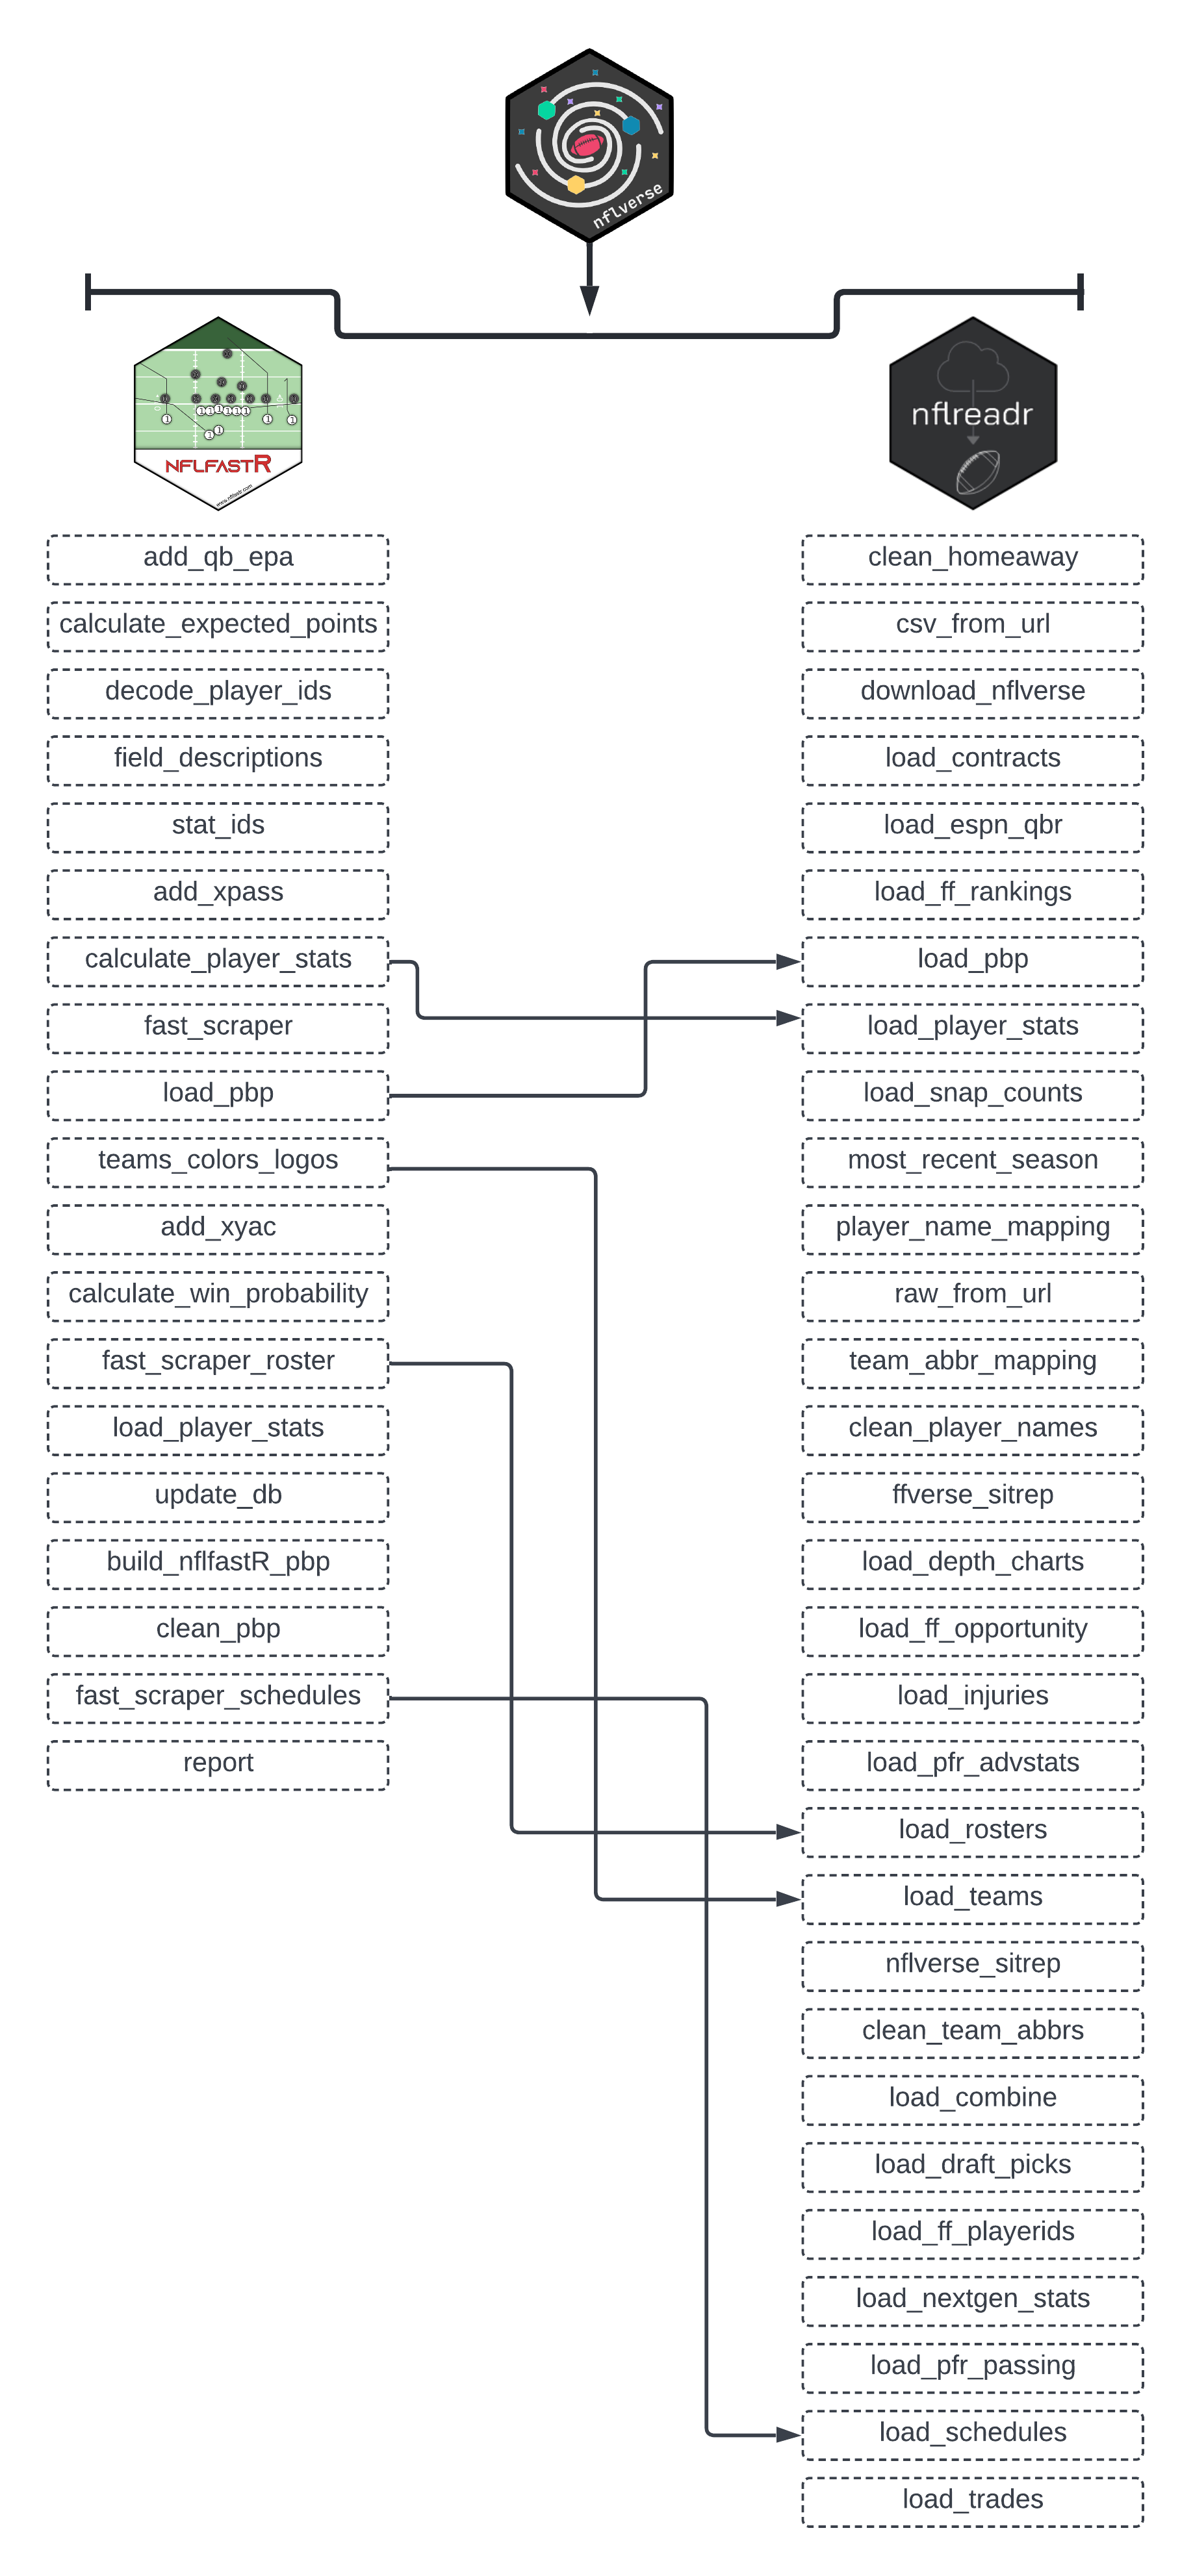
\includegraphics[width=1\textwidth,height=\textheight]{images/updated-diagram.png}

The purpose of this chapter is to explore \texttt{nflreadr} data in an
introductory fashion using, what I believe, are the two most important
functions in the \texttt{nflverse}: (1.) \texttt{load\_player\_stats()}
and (2.) \texttt{load\_pbp()}. It makes the assumption that you are
versed in the R programming language. If you are not, please start with
Chapter 2 where you can learn about R and the \texttt{tidyverse}
language using examples from the \texttt{nflverse}.

\hypertarget{nflreadr-an-introduction-to-the-data}{%
\section{\texorpdfstring{\texttt{nflreadr}: An Introduction to the
Data}{nflreadr: An Introduction to the Data}}\label{nflreadr-an-introduction-to-the-data}}

The most important part of the \texttt{nflverse} is, of course, the
data. To begin, we will examine the core data that underpins the
\texttt{nflverse}: weekly player stats and the more detailed
play-by--play data. Using \texttt{nflreadr}, the end user is able to
collect weekly top-level stats via the \texttt{load\_player\_stats()}
function or the much more robust play-by-play numbers by using the
\texttt{load\_pbp()} function.

As you may imagine, there is a \textbf{very important distinction
between the \texttt{load\_player\_stats()}} \textbf{and
\texttt{load\_pbp()}}. As mentioned, \texttt{load\_player\_stats()} will
provide you with weekly, pre-calculated statistics for either offense or
kicking. Conversely, \texttt{load\_pbp()} will provide over 350 metrics
for every single play of every single game dating back to 1999.

The \texttt{load\_player\_stats()} function includes the following
offensive information:

\begin{Shaded}
\begin{Highlighting}[]
\NormalTok{offensive.stats }\OtherTok{\textless{}{-}}\NormalTok{ nflreadr}\SpecialCharTok{::}\FunctionTok{load\_player\_stats}\NormalTok{(}\DecValTok{2021}\NormalTok{)}

\FunctionTok{ls}\NormalTok{(offensive.stats)}
\end{Highlighting}
\end{Shaded}

\begin{verbatim}
 [1] "air_yards_share"             "attempts"                   
 [3] "carries"                     "completions"                
 [5] "dakota"                      "fantasy_points"             
 [7] "fantasy_points_ppr"          "headshot_url"               
 [9] "interceptions"               "pacr"                       
[11] "passing_2pt_conversions"     "passing_air_yards"          
[13] "passing_epa"                 "passing_first_downs"        
[15] "passing_tds"                 "passing_yards"              
[17] "passing_yards_after_catch"   "player_display_name"        
[19] "player_id"                   "player_name"                
[21] "position"                    "position_group"             
[23] "racr"                        "receiving_2pt_conversions"  
[25] "receiving_air_yards"         "receiving_epa"              
[27] "receiving_first_downs"       "receiving_fumbles"          
[29] "receiving_fumbles_lost"      "receiving_tds"              
[31] "receiving_yards"             "receiving_yards_after_catch"
[33] "recent_team"                 "receptions"                 
[35] "rushing_2pt_conversions"     "rushing_epa"                
[37] "rushing_first_downs"         "rushing_fumbles"            
[39] "rushing_fumbles_lost"        "rushing_tds"                
[41] "rushing_yards"               "sack_fumbles"               
[43] "sack_fumbles_lost"           "sack_yards"                 
[45] "sacks"                       "season"                     
[47] "season_type"                 "special_teams_tds"          
[49] "target_share"                "targets"                    
[51] "week"                        "wopr"                       
\end{verbatim}

As well, switching the \texttt{stat\_type} to ``kicking'' provides the
following information:

\begin{Shaded}
\begin{Highlighting}[]
\NormalTok{kicking.stats }\OtherTok{\textless{}{-}}\NormalTok{ nflreadr}\SpecialCharTok{::}\FunctionTok{load\_player\_stats}\NormalTok{(}\DecValTok{2021}\NormalTok{,}
                                             \AttributeTok{stat\_type =} \StringTok{"kicking"}\NormalTok{)}

\FunctionTok{ls}\NormalTok{(kicking.stats)}
\end{Highlighting}
\end{Shaded}

\begin{verbatim}
 [1] "fg_att"              "fg_blocked"          "fg_blocked_distance"
 [4] "fg_blocked_list"     "fg_long"             "fg_made"            
 [7] "fg_made_0_19"        "fg_made_20_29"       "fg_made_30_39"      
[10] "fg_made_40_49"       "fg_made_50_59"       "fg_made_60_"        
[13] "fg_made_distance"    "fg_made_list"        "fg_missed"          
[16] "fg_missed_0_19"      "fg_missed_20_29"     "fg_missed_30_39"    
[19] "fg_missed_40_49"     "fg_missed_50_59"     "fg_missed_60_"      
[22] "fg_missed_distance"  "fg_missed_list"      "fg_pct"             
[25] "gwfg_att"            "gwfg_blocked"        "gwfg_distance"      
[28] "gwfg_made"           "gwfg_missed"         "pat_att"            
[31] "pat_blocked"         "pat_made"            "pat_missed"         
[34] "pat_pct"             "player_id"           "player_name"        
[37] "season"              "season_type"         "team"               
[40] "week"               
\end{verbatim}

While the data returned is not as rich as the play-by-play data we will
covering next, the \texttt{load\_player\_stats()} function is extremely
helpful when you need to quickly (and correctly!) recreate the official
stats listed on either the NFL's website or on
\href{https://www.pro-football-reference.com/}{Pro Football Reference}.

As an example, let's say you need to get Patrick Mahomes' total passing
yard and attempts from the 2022 season. You could do so via
\texttt{load\_pbp()} but, if you do not need further context (such as
down, distance, quarter, etc.), using \texttt{load\_player\_stats()} is
much more efficient.

\hypertarget{getting-player-stats-via-load_player_stats}{%
\subsection{\texorpdfstring{Getting Player Stats via
\texttt{load\_player\_stats()}}{Getting Player Stats via load\_player\_stats()}}\label{getting-player-stats-via-load_player_stats}}

We can generate a data frame titled \texttt{mahomes\_pyards} but running
the following code:

\begin{Shaded}
\begin{Highlighting}[]
\NormalTok{mahomes\_pyards }\OtherTok{\textless{}{-}}\NormalTok{ nflreadr}\SpecialCharTok{::}\FunctionTok{load\_player\_stats}\NormalTok{(}\AttributeTok{seasons =} \DecValTok{2022}\NormalTok{)}
\end{Highlighting}
\end{Shaded}

In the above example, we specified that the returned data be from the
2022 season. It needs to be noted that running
\texttt{load\_play\_stats()} (without a specific season) will return the
newest season in the data. Moreover, separating two seasons with a colon
(\texttt{:}) will provide multiple seasons of data. In our working
example, the \texttt{mahomes\_pyards} data frame contains statistics for
every player from every week of the 2022 season.

It is important to note that the structure of the data returned by
\texttt{load\_player\_stats()} includes passing yards, rushing yards,
receiving yards, etc. for each player. As a result, the data returns -
for example - the week-by-week statistics for rushing and receiving for
Peyton Manning, not just his passing numbers. Because of this, we can
calculate Peyton's rushing statistics from 2000 to 2022.

\begin{verbatim}
# A tibble: 1 x 4
  carries rushing_yards rushing_tds rush_epa
    <int>         <dbl>       <int>    <dbl>
1     409           531          18   -0.740
\end{verbatim}

Knowing that Peyton's average rushing EPA from 2000 to the end of his
career was -0.740 is not going to win you final Jeopardy nor is it going
to be helpful in any sort of Twitter football discourse. When working
with \texttt{load\_player\_stats()}, it is important that you know the
variable names that are useful to the research you are doing.

\begin{tcolorbox}[enhanced jigsaw, left=2mm, toprule=.15mm, opacitybacktitle=0.6, leftrule=.75mm, bottomrule=.15mm, colbacktitle=quarto-callout-tip-color!10!white, breakable, colback=white, bottomtitle=1mm, toptitle=1mm, title=\textcolor{quarto-callout-tip-color}{\faLightbulb}\hspace{0.5em}{Tip}, coltitle=black, titlerule=0mm, arc=.35mm, opacityback=0, colframe=quarto-callout-tip-color-frame, rightrule=.15mm]

The relevant passing statistics housed in \texttt{load\_player\_stats()}
includes:

\begin{verbatim}
 [1] "completions"               "attempts"                 
 [3] "passing_yards"             "passing_tds"              
 [5] "interceptions"             "sacks"                    
 [7] "sack_yards"                "sack_fumbles"             
 [9] "sack_fumbles_lost"         "passing_air_yards"        
[11] "passing_yards_after_catch" "passing_first_downs"      
[13] "passing_epa"               "passing_2pt_conversions"  
[15] "pacr"                      "dakota"                   
\end{verbatim}

The columns relevant to rushing statistics in
\texttt{load\_player\_stats()} are:

\begin{verbatim}
[1] "carries"                 "rushing_yards"          
[3] "rushing_tds"             "rushing_fumbles"        
[5] "rushing_fumbles_lost"    "rushing_first_downs"    
[7] "rushing_epa"             "rushing_2pt_conversions"
\end{verbatim}

Lastly, the columns for receiving statistics in
\texttt{load\_player\_stats()} include:

\begin{verbatim}
 [1] "receptions"                  "targets"                    
 [3] "receiving_yards"             "receiving_tds"              
 [5] "receiving_fumbles"           "receiving_fumbles_lost"     
 [7] "receiving_air_yards"         "receiving_yards_after_catch"
 [9] "receiving_first_downs"       "receiving_epa"              
[11] "receiving_2pt_conversions"   "racr"                       
[13] "target_share"                "air_yards_share"            
\end{verbatim}

\end{tcolorbox}

Continuing with our above example working with
\texttt{load\_player\_stats()} and Patrick Mahomes, we can find his
total passing yards during the 2022 regular season by using the
\texttt{filter()} function to sort the data for either
\texttt{player\_name} or \texttt{player\_display\_name} as well the the
\texttt{season\_type} and then use \texttt{summarize()} to get the total
of his \texttt{passing\_yards} over the course of the regular season.

\begin{Shaded}
\begin{Highlighting}[]
\NormalTok{mahomes\_pyards }\OtherTok{\textless{}{-}}\NormalTok{ mahomes\_pyards }\SpecialCharTok{\%\textgreater{}\%}
  \FunctionTok{filter}\NormalTok{(player\_name }\SpecialCharTok{==} \StringTok{"P.Mahomes"} \SpecialCharTok{\&}\NormalTok{ season\_type }\SpecialCharTok{==} \StringTok{"REG"}\NormalTok{) }\SpecialCharTok{\%\textgreater{}\%}
  \FunctionTok{summarize}\NormalTok{(}\AttributeTok{passing\_yards =} \FunctionTok{sum}\NormalTok{(passing\_yards))}

\NormalTok{mahomes\_pyards}
\end{Highlighting}
\end{Shaded}

\begin{verbatim}
# A tibble: 1 x 1
  passing_yards
          <dbl>
1          5250
\end{verbatim}

The above code returns a result of 5,250 passing yards which is an exact
match from the data provided by
\href{https://www.pro-football-reference.com/players/M/MahoPa00.htm}{Pro
Football Reference.} In the above example, we used the \texttt{filter()}
function on the \texttt{player\_name} column in the data. You will get
the same result if you replace that with
\texttt{player\_display\_name\ ==\ "Patrick\ Mahomes"}. While there is
no difference in how the data is collected, there will be a difference
if you were to visualize the data frame and wished to display the player
names along with their respective statistics. In most cases, in order to
maintain a clean design, using the \texttt{player\_name} option is best
as it allows you to plot just the player's first initial and last name.

We can build upon the passing yards example to replicate the vast
majority of statistics found in
the\href{https://www.pro-football-reference.com/players/M/MahoPa00.htm\#passing}{``Passing''
data table for Mahomes from Pro Football Reference}.

\begin{Shaded}
\begin{Highlighting}[]
\NormalTok{mahomes\_pfr }\OtherTok{\textless{}{-}}\NormalTok{ nflreadr}\SpecialCharTok{::}\FunctionTok{load\_player\_stats}\NormalTok{(}\AttributeTok{seasons =} \DecValTok{2022}\NormalTok{) }\SpecialCharTok{\%\textgreater{}\%}
  \FunctionTok{filter}\NormalTok{(player\_name }\SpecialCharTok{==} \StringTok{"P.Mahomes"} \SpecialCharTok{\&}\NormalTok{ season\_type }\SpecialCharTok{==} \StringTok{"REG"}\NormalTok{) }\SpecialCharTok{\%\textgreater{}\%}
  \FunctionTok{summarize}\NormalTok{(}
    \AttributeTok{completions =} \FunctionTok{sum}\NormalTok{(completions),}
    \AttributeTok{attempts =} \FunctionTok{sum}\NormalTok{(attempts),}
    \AttributeTok{cmp\_pct =}\NormalTok{ completions }\SpecialCharTok{/}\NormalTok{ attempts,}
    \AttributeTok{yards =} \FunctionTok{sum}\NormalTok{(passing\_yards),}
    \AttributeTok{touchdowns =} \FunctionTok{sum}\NormalTok{(passing\_tds),}
    \AttributeTok{td\_pct =}\NormalTok{ touchdowns }\SpecialCharTok{/}\NormalTok{ attempts }\SpecialCharTok{*} \DecValTok{100}\NormalTok{,}
    \AttributeTok{interceptions =} \FunctionTok{sum}\NormalTok{(interceptions),}
    \AttributeTok{int\_pct =}\NormalTok{ interceptions }\SpecialCharTok{/}\NormalTok{ attempts }\SpecialCharTok{*} \DecValTok{100}\NormalTok{,}
    \AttributeTok{first\_down =} \FunctionTok{sum}\NormalTok{(passing\_first\_downs),}
    \AttributeTok{yards\_attempt =}\NormalTok{ yards }\SpecialCharTok{/}\NormalTok{ attempts,}
    \AttributeTok{adj\_yards\_attempt =}\NormalTok{ (yards }\SpecialCharTok{+} \DecValTok{20} \SpecialCharTok{*}\NormalTok{ touchdowns }\SpecialCharTok{{-}} \DecValTok{45} \SpecialCharTok{*}\NormalTok{ interceptions) }\SpecialCharTok{/}\NormalTok{ attempts,}
    \AttributeTok{yards\_completions =}\NormalTok{ yards }\SpecialCharTok{/}\NormalTok{ completions,}
    \AttributeTok{yards\_game =}\NormalTok{ yards }\SpecialCharTok{/} \DecValTok{17}\NormalTok{,}
    \AttributeTok{sacks =} \FunctionTok{sum}\NormalTok{(sacks),}
    \AttributeTok{sack\_yards =} \FunctionTok{sum}\NormalTok{(sack\_yards),}
    \AttributeTok{sack\_pct =}\NormalTok{ sacks }\SpecialCharTok{/}\NormalTok{ (attempts }\SpecialCharTok{+}\NormalTok{ sacks) }\SpecialCharTok{*} \DecValTok{100}\NormalTok{)}

\NormalTok{mahomes\_pfr}
\end{Highlighting}
\end{Shaded}

\begin{verbatim}
# A tibble: 1 x 16
  complet~1 attem~2 cmp_pct yards touch~3 td_pct inter~4 int_pct first~5 yards~6
      <int>   <int>   <dbl> <dbl>   <int>  <dbl>   <dbl>   <dbl>   <dbl>   <dbl>
1       435     648   0.671  5250      41   6.33      12    1.85     272    8.10
# ... with 6 more variables: adj_yards_attempt <dbl>, yards_completions <dbl>,
#   yards_game <dbl>, sacks <dbl>, sack_yards <dbl>, sack_pct <dbl>, and
#   abbreviated variable names 1: completions, 2: attempts, 3: touchdowns,
#   4: interceptions, 5: first_down, 6: yards_attempt
\end{verbatim}

What if we wanted to find Mahomes' adjusted yards gained per pass
attempt for every one of his seasons between 2018 and 2022? It is as
simple as gathering all the data from years
(\texttt{seasons\ =\ 2018:2022}), using the same \texttt{filter()} from
above, and then using \texttt{group\_by()} on the \texttt{season}
variable.

\begin{Shaded}
\begin{Highlighting}[]
\NormalTok{mahomes\_adjusted\_yards }\OtherTok{\textless{}{-}}\NormalTok{ nflreadr}\SpecialCharTok{::}\FunctionTok{load\_player\_stats}\NormalTok{(}\AttributeTok{seasons =} \DecValTok{2018}\SpecialCharTok{:}\DecValTok{2022}\NormalTok{) }\SpecialCharTok{\%\textgreater{}\%}
  \FunctionTok{filter}\NormalTok{(player\_name }\SpecialCharTok{==} \StringTok{"P.Mahomes"} \SpecialCharTok{\&}\NormalTok{ season\_type }\SpecialCharTok{==} \StringTok{"REG"}\NormalTok{) }\SpecialCharTok{\%\textgreater{}\%}
  \FunctionTok{group\_by}\NormalTok{(season) }\SpecialCharTok{\%\textgreater{}\%}
  \FunctionTok{summarize}\NormalTok{(}
    \AttributeTok{adj\_yards\_attempt =}\NormalTok{ (}\FunctionTok{sum}\NormalTok{(passing\_yards) }\SpecialCharTok{+} \DecValTok{20} \SpecialCharTok{*}
                           \FunctionTok{sum}\NormalTok{(passing\_tds) }\SpecialCharTok{{-}} \DecValTok{45} \SpecialCharTok{*}
                           \FunctionTok{sum}\NormalTok{(interceptions)) }\SpecialCharTok{/} \FunctionTok{sum}\NormalTok{(attempts))}

\NormalTok{mahomes\_adjusted\_yards}
\end{Highlighting}
\end{Shaded}

\begin{verbatim}
# A tibble: 5 x 2
  season adj_yards_attempt
   <int>             <dbl>
1   2018              9.58
2   2019              8.94
3   2020              8.89
4   2021              7.59
5   2022              8.53
\end{verbatim}

Based on the data output, Mahomes' best year for adjusted yards gained
per pass attempt was 2018 with 9.58 adjusted yards. How does this
compare to other quarterbacks from the same season? We can find the
answer by doing slight modifications to our above code. Rather than
filtering the information out to just Patrick Mahomes, we will add the
\texttt{player\_name} variable as the argument in the
\texttt{group\_by()} function.

\begin{Shaded}
\begin{Highlighting}[]
\NormalTok{all\_qbs\_adjusted }\OtherTok{\textless{}{-}}\NormalTok{ nflreadr}\SpecialCharTok{::}\FunctionTok{load\_player\_stats}\NormalTok{(}\AttributeTok{seasons =} \DecValTok{2018}\NormalTok{) }\SpecialCharTok{\%\textgreater{}\%}
  \FunctionTok{filter}\NormalTok{(season\_type }\SpecialCharTok{==} \StringTok{"REG"} \SpecialCharTok{\&}\NormalTok{ position }\SpecialCharTok{==} \StringTok{"QB"}\NormalTok{) }\SpecialCharTok{\%\textgreater{}\%}
  \FunctionTok{group\_by}\NormalTok{(player\_name) }\SpecialCharTok{\%\textgreater{}\%}
  \FunctionTok{summarize}\NormalTok{(}
    \AttributeTok{adj\_yards\_attempt =}\NormalTok{ (}\FunctionTok{sum}\NormalTok{(passing\_yards) }\SpecialCharTok{+} \DecValTok{20} \SpecialCharTok{*}
                           \FunctionTok{sum}\NormalTok{(passing\_tds) }\SpecialCharTok{{-}} \DecValTok{45} \SpecialCharTok{*}
                           \FunctionTok{sum}\NormalTok{(interceptions)) }\SpecialCharTok{/} \FunctionTok{sum}\NormalTok{(attempts)) }\SpecialCharTok{\%\textgreater{}\%}
  \FunctionTok{arrange}\NormalTok{(}\SpecialCharTok{{-}}\NormalTok{adj\_yards\_attempt)}

\NormalTok{all\_qbs\_adjusted}
\end{Highlighting}
\end{Shaded}

\begin{verbatim}
# A tibble: 73 x 2
   player_name   adj_yards_attempt
   <chr>                     <dbl>
 1 N.Sudfeld                 21   
 2 G.Gilbert                 13.3 
 3 M.Barkley                 11.7 
 4 K.Allen                    9.87
 5 C.Henne                    9.67
 6 P.Mahomes                  9.58
 7 M.Glennon                  9.24
 8 D.Brees                    9.01
 9 R.Wilson                   8.98
10 R.Fitzpatrick              8.80
# ... with 63 more rows
\end{verbatim}

Mahomes, with an adjusted yards per pass attempt of 9.58, finishes in
sixth place in the 2018 season behind C. Henne (9.67), K. Allen (9.87),
and then three others that have results between 10 and 20. This is a
situation where I tell my students the results do not pass the ``eye
test.'' Why? It is unlikely that an adjusted yards per pass attempt of
21 and 13.3 for Nate Sudfeld and Garrett Gilbert, respectively, are from
a season worth of data. The results for Kyle Allen and Matt Barkley are
questionable, as well.

\begin{tcolorbox}[enhanced jigsaw, left=2mm, toprule=.15mm, opacitybacktitle=0.6, leftrule=.75mm, bottomrule=.15mm, colbacktitle=quarto-callout-important-color!10!white, breakable, colback=white, bottomtitle=1mm, toptitle=1mm, title=\textcolor{quarto-callout-important-color}{\faExclamation}\hspace{0.5em}{Important}, coltitle=black, titlerule=0mm, arc=.35mm, opacityback=0, colframe=quarto-callout-important-color-frame, rightrule=.15mm]

You will often discover artificially-inflated statistics like above when
the players have limited number of pass attempts/rushing
attempts/receptions/etc. compared to the other players on the list. To
confirm this, we can add \texttt{pass\_attempts\ =\ sum(attempts)} to
the above code to compare the number of attempts Sudfeld and Gilbert had
compared to the rest of the list.

\begin{Shaded}
\begin{Highlighting}[]
\NormalTok{all\_qbs\_adjusted\_with\_attempts }\OtherTok{\textless{}{-}}
\NormalTok{  nflreadr}\SpecialCharTok{::}\FunctionTok{load\_player\_stats}\NormalTok{(}\AttributeTok{seasons =} \DecValTok{2018}\NormalTok{) }\SpecialCharTok{\%\textgreater{}\%}
  \FunctionTok{filter}\NormalTok{(season\_type }\SpecialCharTok{==} \StringTok{"REG"} \SpecialCharTok{\&}\NormalTok{ position }\SpecialCharTok{==} \StringTok{"QB"}\NormalTok{) }\SpecialCharTok{\%\textgreater{}\%}
  \FunctionTok{group\_by}\NormalTok{(player\_name) }\SpecialCharTok{\%\textgreater{}\%}
  \FunctionTok{summarize}\NormalTok{(}
    \AttributeTok{pass\_attempts =} \FunctionTok{sum}\NormalTok{(attempts),}
    \AttributeTok{adj\_yards\_attempt =}\NormalTok{ (}\FunctionTok{sum}\NormalTok{(passing\_yards) }\SpecialCharTok{+} \DecValTok{20} \SpecialCharTok{*}
                           \FunctionTok{sum}\NormalTok{(passing\_tds) }\SpecialCharTok{{-}} \DecValTok{45} \SpecialCharTok{*}
                           \FunctionTok{sum}\NormalTok{(interceptions)) }\SpecialCharTok{/} \FunctionTok{sum}\NormalTok{(attempts)) }\SpecialCharTok{\%\textgreater{}\%}
  \FunctionTok{arrange}\NormalTok{(}\SpecialCharTok{{-}}\NormalTok{adj\_yards\_attempt)}

\NormalTok{all\_qbs\_adjusted\_with\_attempts}
\end{Highlighting}
\end{Shaded}

\begin{verbatim}
# A tibble: 73 x 3
   player_name   pass_attempts adj_yards_attempt
   <chr>                 <int>             <dbl>
 1 N.Sudfeld                 2             21   
 2 G.Gilbert                 3             13.3 
 3 M.Barkley                25             11.7 
 4 K.Allen                  31              9.87
 5 C.Henne                   3              9.67
 6 P.Mahomes               580              9.58
 7 M.Glennon                21              9.24
 8 D.Brees                 489              9.01
 9 R.Wilson                427              8.98
10 R.Fitzpatrick           246              8.80
# ... with 63 more rows
\end{verbatim}

The results are even worse than initially thought. There are a total of
six players with an inflated adjusted yards per pass attempt:

\begin{enumerate}
\def\labelenumi{\arabic{enumi}.}
\tightlist
\item
  Nate Sudfeld (2 attempts, 21 adjusted yards).
\item
  Garrett Gilbert (3 attempts, 13.3 adjusted yards).
\item
  Matt Barkley (25 attempts, 11.7 adjusted yards).
\item
  Kyle Allen (31 attempts, 9.87 adjusted yards).
\item
  Chris Henne (3 attempts, 9.67 adjusted yards).
\end{enumerate}

To remove those players with inflated statistics resulting from a lack
of attempts, we can apply a second \texttt{filter()} at the end of our
above code to limit the results to just those quarterbacks with no less
than 100 pass attempts in the 2018 season.

\begin{Shaded}
\begin{Highlighting}[]
\NormalTok{all\_qbs\_attempts\_100 }\OtherTok{\textless{}{-}}
\NormalTok{  nflreadr}\SpecialCharTok{::}\FunctionTok{load\_player\_stats}\NormalTok{(}\AttributeTok{seasons =} \DecValTok{2018}\NormalTok{) }\SpecialCharTok{\%\textgreater{}\%}
  \FunctionTok{filter}\NormalTok{(season\_type }\SpecialCharTok{==} \StringTok{"REG"} \SpecialCharTok{\&}\NormalTok{ position }\SpecialCharTok{==} \StringTok{"QB"}\NormalTok{) }\SpecialCharTok{\%\textgreater{}\%}
  \FunctionTok{group\_by}\NormalTok{(player\_name) }\SpecialCharTok{\%\textgreater{}\%}
  \FunctionTok{summarize}\NormalTok{(}
    \AttributeTok{pass\_attempts =} \FunctionTok{sum}\NormalTok{(attempts),}
    \AttributeTok{adj\_yards\_attempt =}\NormalTok{ (}\FunctionTok{sum}\NormalTok{(passing\_yards) }\SpecialCharTok{+} \DecValTok{20} \SpecialCharTok{*}
                           \FunctionTok{sum}\NormalTok{(passing\_tds) }\SpecialCharTok{{-}} \DecValTok{45} \SpecialCharTok{*}
                           \FunctionTok{sum}\NormalTok{(interceptions)) }\SpecialCharTok{/} \FunctionTok{sum}\NormalTok{(attempts)) }\SpecialCharTok{\%\textgreater{}\%}
  \FunctionTok{filter}\NormalTok{(pass\_attempts }\SpecialCharTok{\textgreater{}=} \DecValTok{100}\NormalTok{) }\SpecialCharTok{\%\textgreater{}\%}
  \FunctionTok{arrange}\NormalTok{(}\SpecialCharTok{{-}}\NormalTok{adj\_yards\_attempt)}

\NormalTok{all\_qbs\_attempts\_100}
\end{Highlighting}
\end{Shaded}

\end{tcolorbox}

After including a \texttt{filter()} to the code to remove those
quarterbacks with less than 100 attempts, it is clear that Mahomes has
the best adjusted pass yards per attempt (9.58) in the 2018 season with
Drew Brees in second place with 9.01. Based on our previous examples, we
know that a Mahomes 9.58 adjusted pass yards per attempt in 2018 was his
career high (and is also the highest in the 2018 season). How do his
other seasons stack up? Is his lowest adjusted pass yards (7.59) in 2021
still the best among NFL quarterbacks in that specific season?

To find the answer, we can make slight adjustments to our existing code.

\begin{Shaded}
\begin{Highlighting}[]
\NormalTok{best\_adjusted\_yards }\OtherTok{\textless{}{-}}
\NormalTok{  nflreadr}\SpecialCharTok{::}\FunctionTok{load\_player\_stats}\NormalTok{(}\AttributeTok{seasons =} \DecValTok{2018}\SpecialCharTok{:}\DecValTok{2022}\NormalTok{) }\SpecialCharTok{\%\textgreater{}\%}
  \FunctionTok{filter}\NormalTok{(season\_type }\SpecialCharTok{==} \StringTok{"REG"} \SpecialCharTok{\&}\NormalTok{ position }\SpecialCharTok{==} \StringTok{"QB"}\NormalTok{) }\SpecialCharTok{\%\textgreater{}\%}
  \FunctionTok{group\_by}\NormalTok{(season, player\_name) }\SpecialCharTok{\%\textgreater{}\%}
  \FunctionTok{summarize}\NormalTok{(}
    \AttributeTok{pass\_attempts =} \FunctionTok{sum}\NormalTok{(attempts),}
    \AttributeTok{adj\_yards\_attempt =}\NormalTok{ (}\FunctionTok{sum}\NormalTok{(passing\_yards) }\SpecialCharTok{+} \DecValTok{20} \SpecialCharTok{*}
                           \FunctionTok{sum}\NormalTok{(passing\_tds) }\SpecialCharTok{{-}} \DecValTok{45} \SpecialCharTok{*}
                           \FunctionTok{sum}\NormalTok{(interceptions)) }\SpecialCharTok{/} \FunctionTok{sum}\NormalTok{(attempts)) }\SpecialCharTok{\%\textgreater{}\%}
  \FunctionTok{filter}\NormalTok{(pass\_attempts }\SpecialCharTok{\textgreater{}=} \DecValTok{100}\NormalTok{) }\SpecialCharTok{\%\textgreater{}\%}
  \FunctionTok{ungroup}\NormalTok{() }\SpecialCharTok{\%\textgreater{}\%}
  \FunctionTok{group\_by}\NormalTok{(season) }\SpecialCharTok{\%\textgreater{}\%}
  \FunctionTok{filter}\NormalTok{(adj\_yards\_attempt }\SpecialCharTok{==} \FunctionTok{max}\NormalTok{(adj\_yards\_attempt))}
\end{Highlighting}
\end{Shaded}

\begin{verbatim}
`summarise()` has grouped output by 'season'. You can override using the
`.groups` argument.
\end{verbatim}

\begin{Shaded}
\begin{Highlighting}[]
\NormalTok{best\_adjusted\_yards}
\end{Highlighting}
\end{Shaded}

\begin{verbatim}
# A tibble: 5 x 4
# Groups:   season [5]
  season player_name  pass_attempts adj_yards_attempt
   <int> <chr>                <int>             <dbl>
1   2018 P.Mahomes              580              9.58
2   2019 R.Tannehill            286             10.2 
3   2020 A.Rodgers              526              9.57
4   2021 J.Burrow               520              8.96
5   2022 T.Tagovailoa           400              9.22
\end{verbatim}

To get the answer, we've created code that follows along with our prior
examples. However, after using \texttt{filter()} to limit the number of
attempts each quarterback must have, we use \texttt{ungroup()} to remove
the previous grouping between \texttt{season} and \texttt{player\_name}
and then use \texttt{group\_by()} again on just the \texttt{season}
information in the data. After, we use \texttt{filter()} to select just
the highest adjusted yards per attempt for each individual season. As a
result, we can see that Mahomes only led the NFL in this specific metric
in the 2018 season. In fact, between the 2018 and 2022 seasons, Ryan
Tannehill had the highest adjusted yards per attempt with 10.2 (but
notice he had just 286 passing attempts).

As mentioned, the \texttt{load\_player\_stats()} information is provided
on a week-by-week basis. In our above example, we are aggregating all
regular season weeks into a season-long metric. Given the structure of
the data, we can take a similar approach but to determine the leaders on
a week-by-week basis. To showcase this, we can determine the leader in
rushing EPA for every week during the 2022 regular season.

\begin{Shaded}
\begin{Highlighting}[]
\NormalTok{rushing\_epa\_leader }\OtherTok{\textless{}{-}}\NormalTok{ nflreadr}\SpecialCharTok{::}\FunctionTok{load\_player\_stats}\NormalTok{(}\AttributeTok{season =} \DecValTok{2022}\NormalTok{) }\SpecialCharTok{\%\textgreater{}\%}
  \FunctionTok{filter}\NormalTok{(season\_type }\SpecialCharTok{==} \StringTok{"REG"} \SpecialCharTok{\&}\NormalTok{ position }\SpecialCharTok{==} \StringTok{"RB"}\NormalTok{) }\SpecialCharTok{\%\textgreater{}\%}
  \FunctionTok{filter}\NormalTok{(}\SpecialCharTok{!}\FunctionTok{is.na}\NormalTok{(rushing\_epa)) }\SpecialCharTok{\%\textgreater{}\%}
  \FunctionTok{group\_by}\NormalTok{(week, player\_name) }\SpecialCharTok{\%\textgreater{}\%}
  \FunctionTok{summarize}\NormalTok{(}
    \AttributeTok{carries =}\NormalTok{ carries,}
    \AttributeTok{rush\_epa =}\NormalTok{ rushing\_epa) }\SpecialCharTok{\%\textgreater{}\%}
  \FunctionTok{filter}\NormalTok{(carries }\SpecialCharTok{\textgreater{}=} \DecValTok{10}\NormalTok{) }\SpecialCharTok{\%\textgreater{}\%}
  \FunctionTok{ungroup}\NormalTok{() }\SpecialCharTok{\%\textgreater{}\%}
  \FunctionTok{group\_by}\NormalTok{(week) }\SpecialCharTok{\%\textgreater{}\%}
  \FunctionTok{filter}\NormalTok{(rush\_epa }\SpecialCharTok{==} \FunctionTok{max}\NormalTok{(rush\_epa))}
\end{Highlighting}
\end{Shaded}

\begin{verbatim}
# A tibble: 18 x 4
# Groups:   week [18]
    week player_name carries rush_epa
   <int> <chr>         <int>    <dbl>
 1     1 D.Swift          15    10.0 
 2     2 A.Jones          15     8.08
 3     3 C.Patterson      17     5.76
 4     4 R.Penny          17     9.73
 5     5 A.Ekeler         16    11.6 
 6     6 K.Drake          10     6.72
 7     7 J.Jacobs         20     6.93
 8     8 T.Etienne        24     9.68
 9     9 J.Mixon          22    11.3 
10    10 A.Jones          24     5.47
11    11 J.Cook           11     2.92
12    12 M.Sanders        21     6.72
13    13 T.Pollard        12     3.97
14    14 M.Sanders        17     8.95
15    15 T.Allgeier       17    10.5 
16    16 D.Foreman        21     7.22
17    17 A.Ekeler         10    10.0 
18    18 A.Mattison       10     5.85
\end{verbatim}

Rather than using the \texttt{season} variable in the
\texttt{group\_by()} function, we instead use \texttt{week} to calculate
the leader in rushing EPA. The results show that the weekly leader is
varied, with only Austin Ekeler and Aaron Jones appearing on the list
more than once. The Bengals' Joe Mixon produced the largest rushing EPA
in the 2022 season, recording 11.3 in week 9 while James Cook's 2.92
output in week 11 was the ``least'' of the best weekly performances.

Much like we did with the passing statistics, we can use the rushing
data in \texttt{load\_player\_stats()} to replicate the majority found
on Pro Football Reference. To do so, let's use Joe Mixon's week 9
performance from the 2022 season.

\begin{Shaded}
\begin{Highlighting}[]
\NormalTok{mixon\_week\_9 }\OtherTok{\textless{}{-}}\NormalTok{ nflreadr}\SpecialCharTok{::}\FunctionTok{load\_player\_stats}\NormalTok{(}\AttributeTok{seasons =} \DecValTok{2022}\NormalTok{) }\SpecialCharTok{\%\textgreater{}\%}
  \FunctionTok{filter}\NormalTok{(player\_name }\SpecialCharTok{==} \StringTok{"J.Mixon"} \SpecialCharTok{\&}\NormalTok{ week }\SpecialCharTok{==} \DecValTok{9}\NormalTok{) }\SpecialCharTok{\%\textgreater{}\%}
  \FunctionTok{summarize}\NormalTok{(}
    \AttributeTok{rushes =} \FunctionTok{sum}\NormalTok{(carries),}
    \AttributeTok{yards =} \FunctionTok{sum}\NormalTok{(rushing\_yards),}
    \AttributeTok{yards\_att =}\NormalTok{ yards }\SpecialCharTok{/}\NormalTok{ rushes,}
    \AttributeTok{tds =} \FunctionTok{sum}\NormalTok{(rushing\_tds),}
    \AttributeTok{first\_down =} \FunctionTok{sum}\NormalTok{(rushing\_first\_downs))}

\NormalTok{mixon\_week\_9}
\end{Highlighting}
\end{Shaded}

\begin{verbatim}
# A tibble: 1 x 5
  rushes yards yards_att   tds first_down
   <int> <dbl>     <dbl> <int>      <dbl>
1     22   153      6.95     4         12
\end{verbatim}

Mixon gained a total of 153 yards on the ground on 22 carries, which is
just under 7 yards per attempt. Four of those carries resulting in
touchdowns, while 12 of them kept drives alive with first downs. Other
contextual statistics for this performance, such as yards after contact,
are not included in \texttt{load\_player\_stats()} but can be retrieved
using other functions within the \texttt{nflverse()} (which are covered
later in this chapter).

Finally, we can use the \texttt{load\_player\_stats()} function to
explore wide receiver performances. As listed above, the wide receivers
statistics housed within \texttt{load\_player\_stats()} include those to
be expected: yards, touchdowns, air yards, yards after catch, etc.
Rather than working with those in an example, let's use \texttt{wopr}
which stands for \texttt{Weighted\ Opportunity\ Rating}, which is a
weighted average that contextualizes how much value any one wide
receivers bring to a fantasy football team. The equation is already
built into the data, but for clarity it is as follows:

\[
1.5 * target share + 0.7 * air yards share
\]

We can use \texttt{wopr} to determine which wide receiver was the most
valuable to fantasy football owners during the 2022 season.

\begin{Shaded}
\begin{Highlighting}[]
\NormalTok{receivers\_wopr }\OtherTok{\textless{}{-}}\NormalTok{ nflreadr}\SpecialCharTok{::}\FunctionTok{load\_player\_stats}\NormalTok{(}\AttributeTok{seasons =} \DecValTok{2022}\NormalTok{) }\SpecialCharTok{\%\textgreater{}\%}
  \FunctionTok{filter}\NormalTok{(season\_type }\SpecialCharTok{==} \StringTok{"REG"} \SpecialCharTok{\&}\NormalTok{ position }\SpecialCharTok{==} \StringTok{"WR"}\NormalTok{) }\SpecialCharTok{\%\textgreater{}\%}
  \FunctionTok{group\_by}\NormalTok{(player\_name) }\SpecialCharTok{\%\textgreater{}\%}
  \FunctionTok{summarize}\NormalTok{(}
    \AttributeTok{total\_wopr =} \FunctionTok{sum}\NormalTok{(wopr)) }\SpecialCharTok{\%\textgreater{}\%}
  \FunctionTok{arrange}\NormalTok{(}\SpecialCharTok{{-}}\NormalTok{total\_wopr)}

\NormalTok{receivers\_wopr}
\end{Highlighting}
\end{Shaded}

\begin{verbatim}
# A tibble: 225 x 2
   player_name total_wopr
   <chr>            <dbl>
 1 D.Moore           13.9
 2 D.Adams           13.4
 3 T.Hill            12.4
 4 A.Brown           12.2
 5 J.Jefferson       11.9
 6 C.Lamb            11.8
 7 A.Cooper          11.8
 8 D.Johnson         11.2
 9 D.London          10.9
10 D.Metcalf         10.7
# ... with 215 more rows
\end{verbatim}

D.J. Moore led the NFL in the 2022 season with a 13.9 Weighted
Opportunity Rating, followed closely by Davante Adams with 13.4.
However, before deciding that D.J. Moore is worth the number one pick in
your upcoming fantasy football draft, it is worth exploring if there is
a relationship between a high Weight Opportunity Rating and a player's
total fantasy points. To do so, we can take our above code that was used
to gather each player's \texttt{WOPR} over the course of the season and
add \texttt{total\_ff\ =\ sum(fantasy\_points)} and also calculate a new
metric called ``Fantasy Points per Weighted Opportunity'' which is
simply the total of a player's points divided by the \texttt{wopr}.

\begin{Shaded}
\begin{Highlighting}[]
\NormalTok{receivers\_wopr\_ff\_context }\OtherTok{\textless{}{-}}
\NormalTok{  nflreadr}\SpecialCharTok{::}\FunctionTok{load\_player\_stats}\NormalTok{(}\AttributeTok{seasons =} \DecValTok{2022}\NormalTok{) }\SpecialCharTok{\%\textgreater{}\%}
  \FunctionTok{filter}\NormalTok{(season\_type }\SpecialCharTok{==} \StringTok{"REG"} \SpecialCharTok{\&}\NormalTok{ position }\SpecialCharTok{==} \StringTok{"WR"}\NormalTok{) }\SpecialCharTok{\%\textgreater{}\%}
  \FunctionTok{group\_by}\NormalTok{(player\_name) }\SpecialCharTok{\%\textgreater{}\%}
  \FunctionTok{summarize}\NormalTok{(}
    \AttributeTok{total\_wopr =} \FunctionTok{sum}\NormalTok{(wopr),}
    \AttributeTok{total\_ff =} \FunctionTok{sum}\NormalTok{(fantasy\_points),}
    \AttributeTok{ff\_per\_wopr =}\NormalTok{ total\_ff }\SpecialCharTok{/}\NormalTok{ total\_wopr) }\SpecialCharTok{\%\textgreater{}\%}
  \FunctionTok{arrange}\NormalTok{(}\SpecialCharTok{{-}}\NormalTok{total\_wopr)}

\NormalTok{receivers\_wopr\_ff\_context}
\end{Highlighting}
\end{Shaded}

\begin{verbatim}
# A tibble: 225 x 4
   player_name total_wopr total_ff ff_per_wopr
   <chr>            <dbl>    <dbl>       <dbl>
 1 D.Moore           13.9    136.         9.76
 2 D.Adams           13.4    236.        17.6 
 3 T.Hill            12.4    222.        17.9 
 4 A.Brown           12.2    212.        17.4 
 5 J.Jefferson       11.9    241.        20.3 
 6 C.Lamb            11.8    195.        16.5 
 7 A.Cooper          11.8    168         14.2 
 8 D.Johnson         11.2     94.7        8.48
 9 D.London          10.9    107.         9.77
10 D.Metcalf         10.7    137.        12.7 
# ... with 215 more rows
\end{verbatim}

There are several insights evident in the results. Of the top
\texttt{wopr} earners in the 2022 season. only Diontae Johnson scored
fewer fantasy points than D.J. Moore (94.7 to 136). Given the
relationship between \texttt{total\_wopr} and \texttt{total\_ff}, a
lower \texttt{ff\_per\_wopr} is indicative of less stellar play. In this
case, Moore maintained a large amount of both the team's
\texttt{target\_share} and \texttt{air\_yards\_share}, but was not able
to translate that into a higher amount of fantasy points (as evidenced
by a lower \texttt{ff\_per\_wopr} score). On the other hand, Justin
Jefferson's \texttt{ff\_per\_wopr} score of 20.3 argues that he used his
amount of \texttt{target\_share} and \texttt{air\_yards\_share} to
increase the amount of fantasy points he produced.

Based on the above examples, it is clear that the
\texttt{load\_player\_stats()} function is useful when needing to
aggregate statistics on a weekly or season-long basis. While this does
allow for easy matching of official statistics, it does not provide the
ability to add context to the findings. For example, we know that
Patrick Mahomes had the highest adjusted pass yards per attempt during
the 2018 regular season with 9.58. But, what if we wanted to explore
that same metric but only on passes that took place on 3rd down with 10
or less yards to go?

Unfortunately, the \texttt{load\_player\_stats()} function does not
provide ability to distill the statistics into specific situations.
Because of this, we must turn to the \texttt{load\_pbp()} function.

\hypertarget{using-load_pbp-to-add-context-to-statistics}{%
\section{\texorpdfstring{Using \texttt{load\_pbp()} to Add Context to
Statistics}{Using load\_pbp() to Add Context to Statistics}}\label{using-load_pbp-to-add-context-to-statistics}}

Using the \texttt{load\_pbp()} function is preferable when you are
looking to add context to a player's statistics, as the
\texttt{load\_player\_stats()} function is, for all intents and
purposes, aggregated statistics that limit your ability to find deeper
meaning.

The \texttt{load\_pbp()} function provides over 350 various metrics, as
listed below:

\begin{Shaded}
\begin{Highlighting}[]
\NormalTok{pbp.data }\OtherTok{\textless{}{-}}\NormalTok{ nflreadr}\SpecialCharTok{::}\FunctionTok{load\_pbp}\NormalTok{(}\DecValTok{2022}\NormalTok{)}
\FunctionTok{ls}\NormalTok{(pbp.data)}
\end{Highlighting}
\end{Shaded}

\begin{verbatim}
  [1] "aborted_play"                        
  [2] "air_epa"                             
  [3] "air_wpa"                             
  [4] "air_yards"                           
  [5] "assist_tackle"                       
  [6] "assist_tackle_1_player_id"           
  [7] "assist_tackle_1_player_name"         
  [8] "assist_tackle_1_team"                
  [9] "assist_tackle_2_player_id"           
 [10] "assist_tackle_2_player_name"         
 [11] "assist_tackle_2_team"                
 [12] "assist_tackle_3_player_id"           
 [13] "assist_tackle_3_player_name"         
 [14] "assist_tackle_3_team"                
 [15] "assist_tackle_4_player_id"           
 [16] "assist_tackle_4_player_name"         
 [17] "assist_tackle_4_team"                
 [18] "away_coach"                          
 [19] "away_score"                          
 [20] "away_team"                           
 [21] "away_timeouts_remaining"             
 [22] "away_wp"                             
 [23] "away_wp_post"                        
 [24] "blocked_player_id"                   
 [25] "blocked_player_name"                 
 [26] "comp_air_epa"                        
 [27] "comp_air_wpa"                        
 [28] "comp_yac_epa"                        
 [29] "comp_yac_wpa"                        
 [30] "complete_pass"                       
 [31] "cp"                                  
 [32] "cpoe"                                
 [33] "def_wp"                              
 [34] "defensive_extra_point_attempt"       
 [35] "defensive_extra_point_conv"          
 [36] "defensive_two_point_attempt"         
 [37] "defensive_two_point_conv"            
 [38] "defteam"                             
 [39] "defteam_score"                       
 [40] "defteam_score_post"                  
 [41] "defteam_timeouts_remaining"          
 [42] "desc"                                
 [43] "div_game"                            
 [44] "down"                                
 [45] "drive"                               
 [46] "drive_end_transition"                
 [47] "drive_end_yard_line"                 
 [48] "drive_ended_with_score"              
 [49] "drive_first_downs"                   
 [50] "drive_game_clock_end"                
 [51] "drive_game_clock_start"              
 [52] "drive_inside20"                      
 [53] "drive_play_count"                    
 [54] "drive_play_id_ended"                 
 [55] "drive_play_id_started"               
 [56] "drive_quarter_end"                   
 [57] "drive_quarter_start"                 
 [58] "drive_real_start_time"               
 [59] "drive_start_transition"              
 [60] "drive_start_yard_line"               
 [61] "drive_time_of_possession"            
 [62] "drive_yards_penalized"               
 [63] "end_clock_time"                      
 [64] "end_yard_line"                       
 [65] "ep"                                  
 [66] "epa"                                 
 [67] "extra_point_attempt"                 
 [68] "extra_point_prob"                    
 [69] "extra_point_result"                  
 [70] "fantasy"                             
 [71] "fantasy_id"                          
 [72] "fantasy_player_id"                   
 [73] "fantasy_player_name"                 
 [74] "fg_prob"                             
 [75] "field_goal_attempt"                  
 [76] "field_goal_result"                   
 [77] "first_down"                          
 [78] "first_down_pass"                     
 [79] "first_down_penalty"                  
 [80] "first_down_rush"                     
 [81] "fixed_drive"                         
 [82] "fixed_drive_result"                  
 [83] "forced_fumble_player_1_player_id"    
 [84] "forced_fumble_player_1_player_name"  
 [85] "forced_fumble_player_1_team"         
 [86] "forced_fumble_player_2_player_id"    
 [87] "forced_fumble_player_2_player_name"  
 [88] "forced_fumble_player_2_team"         
 [89] "fourth_down_converted"               
 [90] "fourth_down_failed"                  
 [91] "fumble"                              
 [92] "fumble_forced"                       
 [93] "fumble_lost"                         
 [94] "fumble_not_forced"                   
 [95] "fumble_out_of_bounds"                
 [96] "fumble_recovery_1_player_id"         
 [97] "fumble_recovery_1_player_name"       
 [98] "fumble_recovery_1_team"              
 [99] "fumble_recovery_1_yards"             
[100] "fumble_recovery_2_player_id"         
[101] "fumble_recovery_2_player_name"       
[102] "fumble_recovery_2_team"              
[103] "fumble_recovery_2_yards"             
[104] "fumbled_1_player_id"                 
[105] "fumbled_1_player_name"               
[106] "fumbled_1_team"                      
[107] "fumbled_2_player_id"                 
[108] "fumbled_2_player_name"               
[109] "fumbled_2_team"                      
[110] "game_date"                           
[111] "game_half"                           
[112] "game_id"                             
[113] "game_seconds_remaining"              
[114] "game_stadium"                        
[115] "goal_to_go"                          
[116] "half_sack_1_player_id"               
[117] "half_sack_1_player_name"             
[118] "half_sack_2_player_id"               
[119] "half_sack_2_player_name"             
[120] "half_seconds_remaining"              
[121] "home_coach"                          
[122] "home_opening_kickoff"                
[123] "home_score"                          
[124] "home_team"                           
[125] "home_timeouts_remaining"             
[126] "home_wp"                             
[127] "home_wp_post"                        
[128] "id"                                  
[129] "incomplete_pass"                     
[130] "interception"                        
[131] "interception_player_id"              
[132] "interception_player_name"            
[133] "jersey_number"                       
[134] "kick_distance"                       
[135] "kicker_player_id"                    
[136] "kicker_player_name"                  
[137] "kickoff_attempt"                     
[138] "kickoff_downed"                      
[139] "kickoff_fair_catch"                  
[140] "kickoff_in_endzone"                  
[141] "kickoff_inside_twenty"               
[142] "kickoff_out_of_bounds"               
[143] "kickoff_returner_player_id"          
[144] "kickoff_returner_player_name"        
[145] "lateral_interception_player_id"      
[146] "lateral_interception_player_name"    
[147] "lateral_kickoff_returner_player_id"  
[148] "lateral_kickoff_returner_player_name"
[149] "lateral_punt_returner_player_id"     
[150] "lateral_punt_returner_player_name"   
[151] "lateral_receiver_player_id"          
[152] "lateral_receiver_player_name"        
[153] "lateral_receiving_yards"             
[154] "lateral_reception"                   
[155] "lateral_recovery"                    
[156] "lateral_return"                      
[157] "lateral_rush"                        
[158] "lateral_rusher_player_id"            
[159] "lateral_rusher_player_name"          
[160] "lateral_rushing_yards"               
[161] "lateral_sack_player_id"              
[162] "lateral_sack_player_name"            
[163] "location"                            
[164] "name"                                
[165] "nfl_api_id"                          
[166] "no_huddle"                           
[167] "no_score_prob"                       
[168] "old_game_id"                         
[169] "opp_fg_prob"                         
[170] "opp_safety_prob"                     
[171] "opp_td_prob"                         
[172] "order_sequence"                      
[173] "out_of_bounds"                       
[174] "own_kickoff_recovery"                
[175] "own_kickoff_recovery_player_id"      
[176] "own_kickoff_recovery_player_name"    
[177] "own_kickoff_recovery_td"             
[178] "pass"                                
[179] "pass_attempt"                        
[180] "pass_defense_1_player_id"            
[181] "pass_defense_1_player_name"          
[182] "pass_defense_2_player_id"            
[183] "pass_defense_2_player_name"          
[184] "pass_length"                         
[185] "pass_location"                       
[186] "pass_oe"                             
[187] "pass_touchdown"                      
[188] "passer"                              
[189] "passer_id"                           
[190] "passer_jersey_number"                
[191] "passer_player_id"                    
[192] "passer_player_name"                  
[193] "passing_yards"                       
[194] "penalty"                             
[195] "penalty_player_id"                   
[196] "penalty_player_name"                 
[197] "penalty_team"                        
[198] "penalty_type"                        
[199] "penalty_yards"                       
[200] "play"                                
[201] "play_clock"                          
[202] "play_deleted"                        
[203] "play_id"                             
[204] "play_type"                           
[205] "play_type_nfl"                       
[206] "posteam"                             
[207] "posteam_score"                       
[208] "posteam_score_post"                  
[209] "posteam_timeouts_remaining"          
[210] "posteam_type"                        
[211] "punt_attempt"                        
[212] "punt_blocked"                        
[213] "punt_downed"                         
[214] "punt_fair_catch"                     
[215] "punt_in_endzone"                     
[216] "punt_inside_twenty"                  
[217] "punt_out_of_bounds"                  
[218] "punt_returner_player_id"             
[219] "punt_returner_player_name"           
[220] "punter_player_id"                    
[221] "punter_player_name"                  
[222] "qb_dropback"                         
[223] "qb_epa"                              
[224] "qb_hit"                              
[225] "qb_hit_1_player_id"                  
[226] "qb_hit_1_player_name"                
[227] "qb_hit_2_player_id"                  
[228] "qb_hit_2_player_name"                
[229] "qb_kneel"                            
[230] "qb_scramble"                         
[231] "qb_spike"                            
[232] "qtr"                                 
[233] "quarter_end"                         
[234] "quarter_seconds_remaining"           
[235] "receiver"                            
[236] "receiver_id"                         
[237] "receiver_jersey_number"              
[238] "receiver_player_id"                  
[239] "receiver_player_name"                
[240] "receiving_yards"                     
[241] "replay_or_challenge"                 
[242] "replay_or_challenge_result"          
[243] "result"                              
[244] "return_team"                         
[245] "return_touchdown"                    
[246] "return_yards"                        
[247] "roof"                                
[248] "run_gap"                             
[249] "run_location"                        
[250] "rush"                                
[251] "rush_attempt"                        
[252] "rush_touchdown"                      
[253] "rusher"                              
[254] "rusher_id"                           
[255] "rusher_jersey_number"                
[256] "rusher_player_id"                    
[257] "rusher_player_name"                  
[258] "rushing_yards"                       
[259] "sack"                                
[260] "sack_player_id"                      
[261] "sack_player_name"                    
[262] "safety"                              
[263] "safety_player_id"                    
[264] "safety_player_name"                  
[265] "safety_prob"                         
[266] "score_differential"                  
[267] "score_differential_post"             
[268] "season"                              
[269] "season_type"                         
[270] "series"                              
[271] "series_result"                       
[272] "series_success"                      
[273] "shotgun"                             
[274] "side_of_field"                       
[275] "solo_tackle"                         
[276] "solo_tackle_1_player_id"             
[277] "solo_tackle_1_player_name"           
[278] "solo_tackle_1_team"                  
[279] "solo_tackle_2_player_id"             
[280] "solo_tackle_2_player_name"           
[281] "solo_tackle_2_team"                  
[282] "sp"                                  
[283] "special"                             
[284] "special_teams_play"                  
[285] "spread_line"                         
[286] "st_play_type"                        
[287] "stadium"                             
[288] "stadium_id"                          
[289] "start_time"                          
[290] "success"                             
[291] "surface"                             
[292] "tackle_for_loss_1_player_id"         
[293] "tackle_for_loss_1_player_name"       
[294] "tackle_for_loss_2_player_id"         
[295] "tackle_for_loss_2_player_name"       
[296] "tackle_with_assist"                  
[297] "tackle_with_assist_1_player_id"      
[298] "tackle_with_assist_1_player_name"    
[299] "tackle_with_assist_1_team"           
[300] "tackle_with_assist_2_player_id"      
[301] "tackle_with_assist_2_player_name"    
[302] "tackle_with_assist_2_team"           
[303] "tackled_for_loss"                    
[304] "td_player_id"                        
[305] "td_player_name"                      
[306] "td_prob"                             
[307] "td_team"                             
[308] "temp"                                
[309] "third_down_converted"                
[310] "third_down_failed"                   
[311] "time"                                
[312] "time_of_day"                         
[313] "timeout"                             
[314] "timeout_team"                        
[315] "total"                               
[316] "total_away_comp_air_epa"             
[317] "total_away_comp_air_wpa"             
[318] "total_away_comp_yac_epa"             
[319] "total_away_comp_yac_wpa"             
[320] "total_away_epa"                      
[321] "total_away_pass_epa"                 
[322] "total_away_pass_wpa"                 
[323] "total_away_raw_air_epa"              
[324] "total_away_raw_air_wpa"              
[325] "total_away_raw_yac_epa"              
[326] "total_away_raw_yac_wpa"              
[327] "total_away_rush_epa"                 
[328] "total_away_rush_wpa"                 
[329] "total_away_score"                    
[330] "total_home_comp_air_epa"             
[331] "total_home_comp_air_wpa"             
[332] "total_home_comp_yac_epa"             
[333] "total_home_comp_yac_wpa"             
[334] "total_home_epa"                      
[335] "total_home_pass_epa"                 
[336] "total_home_pass_wpa"                 
[337] "total_home_raw_air_epa"              
[338] "total_home_raw_air_wpa"              
[339] "total_home_raw_yac_epa"              
[340] "total_home_raw_yac_wpa"              
[341] "total_home_rush_epa"                 
[342] "total_home_rush_wpa"                 
[343] "total_home_score"                    
[344] "total_line"                          
[345] "touchback"                           
[346] "touchdown"                           
[347] "two_point_attempt"                   
[348] "two_point_conv_result"               
[349] "two_point_conversion_prob"           
[350] "vegas_home_wp"                       
[351] "vegas_home_wpa"                      
[352] "vegas_wp"                            
[353] "vegas_wpa"                           
[354] "weather"                             
[355] "week"                                
[356] "wind"                                
[357] "wp"                                  
[358] "wpa"                                 
[359] "xpass"                               
[360] "xyac_epa"                            
[361] "xyac_fd"                             
[362] "xyac_mean_yardage"                   
[363] "xyac_median_yardage"                 
[364] "xyac_success"                        
[365] "yac_epa"                             
[366] "yac_wpa"                             
[367] "yardline_100"                        
[368] "yards_after_catch"                   
[369] "yards_gained"                        
[370] "ydsnet"                              
[371] "ydstogo"                             
[372] "yrdln"                               
\end{verbatim}

The amount of information contained in the \texttt{nflverse}
play-by-play data can be overwhelming. Luckily, the \texttt{nflreadr}
website includes a searchable directory of all the variables with a
brief description of what each one means. You can visit that here:
\href{https://nflreadr.nflverse.com/articles/dictionary_pbp.html}{nflreadr
Field Descriptions}.

We can recreate our examination of 2018 adjusted pass yards per attempt
to just those passes on 3rd down with 10 or less yards to go by running
the following code:

\begin{Shaded}
\begin{Highlighting}[]
\NormalTok{pbp }\OtherTok{\textless{}{-}}\NormalTok{ nflreadr}\SpecialCharTok{::}\FunctionTok{load\_pbp}\NormalTok{(}\DecValTok{2018}\NormalTok{) }\SpecialCharTok{\%\textgreater{}\%}
  \FunctionTok{filter}\NormalTok{(season\_type }\SpecialCharTok{==} \StringTok{"REG"}\NormalTok{)}

\NormalTok{adjusted\_yards }\OtherTok{\textless{}{-}}\NormalTok{ pbp }\SpecialCharTok{\%\textgreater{}\%}
  \FunctionTok{group\_by}\NormalTok{(passer\_player\_name) }\SpecialCharTok{\%\textgreater{}\%}
  \FunctionTok{filter}\NormalTok{(down }\SpecialCharTok{==} \DecValTok{3} \SpecialCharTok{\&}\NormalTok{ ydstogo }\SpecialCharTok{\textless{}=} \DecValTok{10}\NormalTok{) }\SpecialCharTok{\%\textgreater{}\%}
  \FunctionTok{filter}\NormalTok{(complete\_pass }\SpecialCharTok{==} \DecValTok{1} \SpecialCharTok{|}\NormalTok{ incomplete\_pass }\SpecialCharTok{==} \DecValTok{1} \SpecialCharTok{|}
\NormalTok{           interception }\SpecialCharTok{==} \DecValTok{1} \SpecialCharTok{\&} 
           \SpecialCharTok{!}\FunctionTok{is.na}\NormalTok{(down)) }\SpecialCharTok{\%\textgreater{}\%}
  \FunctionTok{summarize}\NormalTok{(}
    \AttributeTok{total\_attempts =} \FunctionTok{n}\NormalTok{(),}
    \AttributeTok{adj\_yards =}\NormalTok{ (}\FunctionTok{sum}\NormalTok{(yards\_gained) }\SpecialCharTok{+} \DecValTok{20} \SpecialCharTok{*} \FunctionTok{sum}\NormalTok{(touchdown }\SpecialCharTok{==} \DecValTok{1}\NormalTok{) }\SpecialCharTok{{-}} \DecValTok{45} \SpecialCharTok{*} 
                   \FunctionTok{sum}\NormalTok{(interception }\SpecialCharTok{==} \DecValTok{1}\NormalTok{)) }\SpecialCharTok{/}\NormalTok{ total\_attempts) }\SpecialCharTok{\%\textgreater{}\%}
  \FunctionTok{filter}\NormalTok{(total\_attempts }\SpecialCharTok{\textgreater{}=} \DecValTok{50}\NormalTok{) }\SpecialCharTok{\%\textgreater{}\%}
  \FunctionTok{arrange}\NormalTok{(}\SpecialCharTok{{-}}\NormalTok{adj\_yards)}

\NormalTok{adjusted\_yards}
\end{Highlighting}
\end{Shaded}

\begin{verbatim}
# A tibble: 32 x 3
   passer_player_name total_attempts adj_yards
   <chr>                       <int>     <dbl>
 1 A.Rodgers                      98     11.3 
 2 P.Mahomes                     102     10.3 
 3 R.Wilson                      104     10.3 
 4 E.Manning                     119      9.18
 5 M.Mariota                      79      8.43
 6 M.Ryan                        117      8.26
 7 J.Winston                      66      8.05
 8 D.Brees                        97      7.99
 9 D.Prescott                    104      7.87
10 J.Flacco                       74      7.84
# ... with 22 more rows
\end{verbatim}

Because the \texttt{load\_pbp()} data is not pre-aggregated, we must do
a bit of the work ourselves before we are able to achieve our answer. To
start, we load the 2018 play-by-play data into a data frame titled
\texttt{pbp} but using the \texttt{load\_pbp()} function with the
\texttt{season} argument set to ``2018.'' As well, we use the
\texttt{filter()} function to make sure the data gathered into our
\texttt{pbp} data frame is only the regular season statistics. Once the
play-by-play is loaded, we create a data frame off of it titled
\texttt{adjusted\_yards} wherein we use \texttt{group\_by()} to
calculate the metric for each individual quarterback, then ensure that
we are collecting the play-by-play data for only those plays that took
place on 3rd down with ten or less yards to go.

We then use a second \texttt{filter()} to gather those plays where
\texttt{complete\_pass\ ==\ 1} \emph{or}
\texttt{incomplete\_pass\ ==\ 1} \emph{or} \texttt{interception\ ==\ 1}
\emph{and} the \texttt{down} is not missing (which usually indicates a
2-point conversion attempt). As a result, each quarterback has an exact
match to the number of complete passes, attempts, and interceptions as
found in the official statistics of the season.

Despite leading the league in adjusted pass yard per attempt in 2018,
Mahomes finished a whole yard behind Aaron Rodgers when exploring the
same metric on 3rd down with 10 or less yards to go (and was tied for
second place with Russel Wilson).

\begin{tcolorbox}[enhanced jigsaw, left=2mm, toprule=.15mm, opacitybacktitle=0.6, leftrule=.75mm, bottomrule=.15mm, colbacktitle=quarto-callout-tip-color!10!white, breakable, colback=white, bottomtitle=1mm, toptitle=1mm, title=\textcolor{quarto-callout-tip-color}{\faLightbulb}\hspace{0.5em}{Tip}, coltitle=black, titlerule=0mm, arc=.35mm, opacityback=0, colframe=quarto-callout-tip-color-frame, rightrule=.15mm]

Why is it necessary to use such a long list of specifications in the
\texttt{filter()} function in order to match the official QB statistics
found elsewhere?

That is a good question, especially since there are other variables
within the play-by-play data that would seemingly return the correct
results (such as \texttt{pass\ ==\ 1} or
\texttt{play\_type\ ==\ "pass"}. We can view the differences in all
three methods by doing the following.

\begin{Shaded}
\begin{Highlighting}[]
\NormalTok{pbp }\OtherTok{\textless{}{-}}\NormalTok{ nflreadr}\SpecialCharTok{::}\FunctionTok{load\_pbp}\NormalTok{(}\DecValTok{2018}\NormalTok{) }\SpecialCharTok{\%\textgreater{}\%}
  \FunctionTok{filter}\NormalTok{(season\_type }\SpecialCharTok{==} \StringTok{"REG"}\NormalTok{)}

\NormalTok{pbp }\SpecialCharTok{\%\textgreater{}\%}
  \FunctionTok{filter}\NormalTok{(complete\_pass }\SpecialCharTok{==} \DecValTok{1} \SpecialCharTok{|}\NormalTok{ incomplete\_pass }\SpecialCharTok{==} \DecValTok{1} \SpecialCharTok{|}
\NormalTok{           interception }\SpecialCharTok{==} \DecValTok{1} \SpecialCharTok{\&}
           \SpecialCharTok{!}\FunctionTok{is.na}\NormalTok{(down)) }\SpecialCharTok{\%\textgreater{}\%}
  \FunctionTok{filter}\NormalTok{(passer\_player\_name }\SpecialCharTok{==} \StringTok{"P.Mahomes"}\NormalTok{) }\SpecialCharTok{\%\textgreater{}\%}
  \FunctionTok{summarize}\NormalTok{(}\AttributeTok{total\_attempts =} \FunctionTok{n}\NormalTok{())}
\end{Highlighting}
\end{Shaded}

\begin{verbatim}
# A tibble: 1 x 1
  total_attempts
           <int>
1            580
\end{verbatim}

\begin{Shaded}
\begin{Highlighting}[]
\NormalTok{pass\_numbers }\OtherTok{\textless{}{-}}\NormalTok{ pbp }\SpecialCharTok{\%\textgreater{}\%}
  \FunctionTok{filter}\NormalTok{(passer\_player\_name }\SpecialCharTok{==} \StringTok{"P.Mahomes"}\NormalTok{) }\SpecialCharTok{\%\textgreater{}\%}
  \FunctionTok{summarize}\NormalTok{(}
    \AttributeTok{using\_pass =} \FunctionTok{sum}\NormalTok{(pass }\SpecialCharTok{==} \DecValTok{1}\NormalTok{, }\AttributeTok{na.rm =} \ConstantTok{TRUE}\NormalTok{),}
    \AttributeTok{using\_playtype =} \FunctionTok{sum}\NormalTok{(play\_type }\SpecialCharTok{==} \StringTok{"pass"}\NormalTok{),}
    \AttributeTok{using\_filter =} \DecValTok{580}\NormalTok{)}

\NormalTok{pass\_numbers}
\end{Highlighting}
\end{Shaded}

\begin{verbatim}
# A tibble: 1 x 3
  using_pass using_playtype using_filter
       <int>          <int>        <dbl>
1        606            606          580
\end{verbatim}

We know that Patrick Mahomes attempted 580 passes during the 2022
regular season. We can match that number exactly using the
\texttt{filter()} method for \texttt{complete\_pass},
\texttt{incomplete\_pass}, \texttt{interception}, and removing plays
with a missing \texttt{down} observation. When trying to replicate this
number using either the \texttt{pass\ ==\ 1} variable in the
play-by-play data or \texttt{play\_type\ ==\ "pass"}, we get just over
20 more passes than expected.

The main reason for this is the inclusion of the \texttt{qb\_spike},
\texttt{qb\_scramble}, and \texttt{sack} variables. We can actually use
the code above that was used to create the \texttt{pass\_numbers} data
frame, add an additional \texttt{filter()} to account for these, and get
the correct number of passing attempts for each method.

\begin{Shaded}
\begin{Highlighting}[]
\NormalTok{pass\_numbers\_correct }\OtherTok{\textless{}{-}}\NormalTok{ pbp }\SpecialCharTok{\%\textgreater{}\%}
  \FunctionTok{filter}\NormalTok{(passer\_player\_name }\SpecialCharTok{==} \StringTok{"P.Mahomes"}\NormalTok{) }\SpecialCharTok{\%\textgreater{}\%}
  \FunctionTok{filter}\NormalTok{(qb\_spike }\SpecialCharTok{==} \DecValTok{0} \SpecialCharTok{\&}\NormalTok{ qb\_scramble }\SpecialCharTok{==} \DecValTok{0} \SpecialCharTok{\&}\NormalTok{ sack }\SpecialCharTok{==} \DecValTok{0}\NormalTok{) }\SpecialCharTok{\%\textgreater{}\%}
  \FunctionTok{summarize}\NormalTok{(}
    \AttributeTok{using\_pass =} \FunctionTok{sum}\NormalTok{(pass }\SpecialCharTok{==} \DecValTok{1}\NormalTok{, }\AttributeTok{na.rm =} \ConstantTok{TRUE}\NormalTok{),}
    \AttributeTok{using\_playtype =} \FunctionTok{sum}\NormalTok{(play\_type }\SpecialCharTok{==} \StringTok{"pass"}\NormalTok{),}
    \AttributeTok{using\_filter =} \DecValTok{580}\NormalTok{)}

\NormalTok{pass\_numbers\_correct}
\end{Highlighting}
\end{Shaded}

\begin{verbatim}
# A tibble: 1 x 3
  using_pass using_playtype using_filter
       <int>          <int>        <dbl>
1        580            580          580
\end{verbatim}

By using \texttt{filter()} to remove any play that included a QB spike,
a QB scramble, or a sack, we get 580 attempts when using both
\texttt{pass\ ==\ 1} and \texttt{play\_type\ ==\ "pass"} which
replicates the official statistics from the 2018 season for Patrick
Mahomes.

\textbf{\emph{What about the use of \texttt{passer}
vs.~\texttt{passer\_player\_name}?}}

It is also important to remember that you will receive differing numbers
based on your use of \texttt{passer} and \texttt{passer\_player\_name}.
The \texttt{passer} variable is created internally by the
\texttt{nflverse} system and is used to ``mimic'' the statistics without
spikes, scrambles, or sacks in the data. The
\texttt{passer\_player\_name} variable comes from the official
statistics and inherently includes this information.

The following, with the first method using \texttt{group\_by(passer)}
and the second using \texttt{group\_by(passer\_player\_name)} returns
differing results.

\begin{Shaded}
\begin{Highlighting}[]
\NormalTok{passer\_grouping }\OtherTok{\textless{}{-}}\NormalTok{ pbp }\SpecialCharTok{\%\textgreater{}\%}
  \FunctionTok{filter}\NormalTok{(complete\_pass }\SpecialCharTok{==} \DecValTok{1} \SpecialCharTok{|}
\NormalTok{           incomplete\_pass }\SpecialCharTok{==} \DecValTok{1} \SpecialCharTok{|}
\NormalTok{           interception }\SpecialCharTok{==} \DecValTok{1} \SpecialCharTok{\&} \SpecialCharTok{!}\FunctionTok{is.na}\NormalTok{(down)) }\SpecialCharTok{\%\textgreater{}\%}
  \FunctionTok{group\_by}\NormalTok{(passer) }\SpecialCharTok{\%\textgreater{}\%}
  \FunctionTok{summarize}\NormalTok{(}\AttributeTok{total\_attempts =} \FunctionTok{n}\NormalTok{()) }\SpecialCharTok{\%\textgreater{}\%}
  \FunctionTok{arrange}\NormalTok{(}\SpecialCharTok{{-}}\NormalTok{total\_attempts) }\SpecialCharTok{\%\textgreater{}\%}
  \FunctionTok{slice}\NormalTok{(}\DecValTok{1}\SpecialCharTok{:}\DecValTok{5}\NormalTok{)}

\NormalTok{passer\_player\_grouping }\OtherTok{\textless{}{-}}\NormalTok{ pbp }\SpecialCharTok{\%\textgreater{}\%}
  \FunctionTok{filter}\NormalTok{(complete\_pass }\SpecialCharTok{==} \DecValTok{1} \SpecialCharTok{|}
\NormalTok{           incomplete\_pass }\SpecialCharTok{==} \DecValTok{1} \SpecialCharTok{|}
\NormalTok{           interception }\SpecialCharTok{==} \DecValTok{1} \SpecialCharTok{\&} \SpecialCharTok{!}\FunctionTok{is.na}\NormalTok{(down)) }\SpecialCharTok{\%\textgreater{}\%}
  \FunctionTok{group\_by}\NormalTok{(passer\_player\_name) }\SpecialCharTok{\%\textgreater{}\%}
  \FunctionTok{summarize}\NormalTok{(}\AttributeTok{total\_attempts =} \FunctionTok{n}\NormalTok{()) }\SpecialCharTok{\%\textgreater{}\%}
  \FunctionTok{arrange}\NormalTok{(}\SpecialCharTok{{-}}\NormalTok{total\_attempts) }\SpecialCharTok{\%\textgreater{}\%}
  \FunctionTok{slice}\NormalTok{(}\DecValTok{1}\SpecialCharTok{:}\DecValTok{5}\NormalTok{)}

\NormalTok{passer\_grouping}
\end{Highlighting}
\end{Shaded}

\begin{verbatim}
# A tibble: 5 x 2
  passer           total_attempts
  <chr>                     <int>
1 B.Roethlisberger            672
2 A.Luck                      637
3 M.Ryan                      607
4 K.Cousins                   603
5 A.Rodgers                   595
\end{verbatim}

\begin{Shaded}
\begin{Highlighting}[]
\NormalTok{passer\_player\_grouping}
\end{Highlighting}
\end{Shaded}

\begin{verbatim}
# A tibble: 5 x 2
  passer_player_name total_attempts
  <chr>                       <int>
1 B.Roethlisberger              675
2 A.Luck                        639
3 M.Ryan                        608
4 K.Cousins                     606
5 A.Rodgers                     597
\end{verbatim}

When grouping by \texttt{passer}, we get a total attempts of 672 for Ben
Roethlisberger. That number increases to 675 when grouping by
\texttt{passer\_player\_name}. Again, this is because the
\texttt{passer} variable is created by the \texttt{nflverse} and
automatically removes spikes, scrambles, and sacks while
\texttt{passer\_player\_name} includes all three.

We can run the following code to determine where the difference of three
passing attempts is coming from between \texttt{passer} and
\texttt{passer\_player\_name}.

\begin{Shaded}
\begin{Highlighting}[]
\NormalTok{roethlisberger\_difference }\OtherTok{\textless{}{-}}\NormalTok{ pbp }\SpecialCharTok{\%\textgreater{}\%}
  \FunctionTok{filter}\NormalTok{(complete\_pass }\SpecialCharTok{==} \DecValTok{1} \SpecialCharTok{|}
\NormalTok{           incomplete\_pass }\SpecialCharTok{==} \DecValTok{1} \SpecialCharTok{|}
\NormalTok{           interception }\SpecialCharTok{==} \DecValTok{1} \SpecialCharTok{\&} \SpecialCharTok{!}\FunctionTok{is.na}\NormalTok{(down)) }\SpecialCharTok{\%\textgreater{}\%}
  \FunctionTok{group\_by}\NormalTok{(passer\_player\_name) }\SpecialCharTok{\%\textgreater{}\%}
  \FunctionTok{summarize}\NormalTok{(}\AttributeTok{total\_attempts =} \FunctionTok{n}\NormalTok{(),}
            \AttributeTok{spikes =} \FunctionTok{sum}\NormalTok{(qb\_spike }\SpecialCharTok{==} \DecValTok{1}\NormalTok{),}
            \AttributeTok{scramble =} \FunctionTok{sum}\NormalTok{(qb\_scramble }\SpecialCharTok{==} \DecValTok{1}\NormalTok{),}
            \AttributeTok{sacks =} \FunctionTok{sum}\NormalTok{(sack }\SpecialCharTok{==} \DecValTok{1}\NormalTok{)) }\SpecialCharTok{\%\textgreater{}\%}
  \FunctionTok{arrange}\NormalTok{(}\SpecialCharTok{{-}}\NormalTok{total\_attempts) }\SpecialCharTok{\%\textgreater{}\%}
  \FunctionTok{slice}\NormalTok{(}\DecValTok{1}\SpecialCharTok{:}\DecValTok{5}\NormalTok{)}

\NormalTok{roethlisberger\_difference}
\end{Highlighting}
\end{Shaded}

\begin{verbatim}
# A tibble: 5 x 5
  passer_player_name total_attempts spikes scramble sacks
  <chr>                       <int>  <int>    <int> <int>
1 B.Roethlisberger              675      3        0     0
2 A.Luck                        639      2        0     0
3 M.Ryan                        608      1        0     0
4 K.Cousins                     606      3        0     0
5 A.Rodgers                     597      2        0     0
\end{verbatim}

In the case of Roethlisberger, the three pass attempt difference was the
result of the \texttt{passer\_player\_name} grouping including three QB
spikes in the data. \textbf{Aside from when attempting to replicate the
official statistics, it is better to use just \texttt{passer} as it
removes those instances where a QB spike, scramble, or sack my skew the
results of your data.}

\end{tcolorbox}

To continue working with \texttt{load\_pbp()} data, let's create a
metric that examines a QB's aggressiveness on 3rd down passing attempts.
The metric is designed to determine which QBs in the NFL are most
aggressive in 3rd down situations by gauging how often they throw the
ball to, or pass, the first down line. It is an interesting metric to
explore as, just like many metrics in the NFL, not all air yards are
created equal. For example, eight air yards on 1st and 10 are less
valuable than the same eight air yards on 3rd and 5.

\begin{Shaded}
\begin{Highlighting}[]
\NormalTok{pbp }\OtherTok{\textless{}{-}}\NormalTok{ nflreadr}\SpecialCharTok{::}\FunctionTok{load\_pbp}\NormalTok{(}\DecValTok{2022}\NormalTok{)}

\NormalTok{aggressiveness }\OtherTok{\textless{}{-}}\NormalTok{ pbp }\SpecialCharTok{\%\textgreater{}\%}
  \FunctionTok{filter}\NormalTok{(complete\_pass }\SpecialCharTok{==} \DecValTok{1} \SpecialCharTok{|}
\NormalTok{           incomplete\_pass }\SpecialCharTok{==} \DecValTok{1} \SpecialCharTok{|}
\NormalTok{           interception }\SpecialCharTok{==} \DecValTok{1} \SpecialCharTok{\&}
           \SpecialCharTok{!}\FunctionTok{is.na}\NormalTok{(down)) }\SpecialCharTok{\%\textgreater{}\%}
  \FunctionTok{filter}\NormalTok{(down }\SpecialCharTok{==} \DecValTok{3} \SpecialCharTok{\&}\NormalTok{ ydstogo }\SpecialCharTok{\textgreater{}=} \DecValTok{5} \SpecialCharTok{\&}\NormalTok{ ydstogo }\SpecialCharTok{\textless{}=} \DecValTok{10}\NormalTok{) }\SpecialCharTok{\%\textgreater{}\%}
  \FunctionTok{group\_by}\NormalTok{(passer) }\SpecialCharTok{\%\textgreater{}\%}
  \FunctionTok{summarize}\NormalTok{(}
    \AttributeTok{team =} \FunctionTok{last}\NormalTok{(posteam),}
    \AttributeTok{total =} \FunctionTok{n}\NormalTok{(),}
    \AttributeTok{aggressive =} \FunctionTok{sum}\NormalTok{(air\_yards }\SpecialCharTok{\textgreater{}=}\NormalTok{ ydstogo, }\AttributeTok{na.rm =} \ConstantTok{TRUE}\NormalTok{),}
    \AttributeTok{percentage =}\NormalTok{ aggressive }\SpecialCharTok{/}\NormalTok{ total) }\SpecialCharTok{\%\textgreater{}\%}
  \FunctionTok{filter}\NormalTok{(total }\SpecialCharTok{\textgreater{}=} \DecValTok{50}\NormalTok{) }\SpecialCharTok{\%\textgreater{}\%}
  \FunctionTok{arrange}\NormalTok{(}\SpecialCharTok{{-}}\NormalTok{percentage) }\SpecialCharTok{\%\textgreater{}\%}
  \FunctionTok{slice}\NormalTok{(}\DecValTok{1}\SpecialCharTok{:}\DecValTok{10}\NormalTok{)}

\NormalTok{aggressiveness}
\end{Highlighting}
\end{Shaded}

\begin{verbatim}
# A tibble: 10 x 5
   passer    team  total aggressive percentage
   <chr>     <chr> <int>      <int>      <dbl>
 1 P.Mahomes KC       75         55      0.733
 2 K.Pickett PIT      54         36      0.667
 3 M.Jones   NE       56         36      0.643
 4 D.Carr    LV       74         47      0.635
 5 R.Wilson  DEN      63         40      0.635
 6 G.Smith   SEA      65         41      0.631
 7 A.Dalton  NO       55         34      0.618
 8 J.Hurts   PHI      65         40      0.615
 9 K.Cousins MIN      84         51      0.607
10 J.Allen   BUF      61         35      0.574
\end{verbatim}

Following our above example, we use \texttt{filter()} on the
play-by-play data to calculate the total number of attempts for each
quarterback on 3rd down when there were between 5 and 10 yards to go for
a first down. Because we want to make sure we are not gathering attempts
with spikes, scrambles, etc., we use \texttt{passer} in the
\texttt{group\_by()} function and then calculate the \texttt{total}
attempts for each quarterback. After, we find the total number of times
each quarterback was \texttt{aggressive} by finding the sum of attempts
where the \texttt{air\_yards} of the pass were greater than or equal to
the required \texttt{ydstogo}. The two numbers are then divided
(\texttt{aggressive} / \texttt{total}) to get each quarterback's
percentage.

As you can see in the output of \texttt{aggressiveness}, Mahomes was the
most aggressive quarterback in 3rd down passing situation in the 2022
season, passing to, or beyond, the line of gain just over 73\% of the
time.

One item to consider, however, is the concept of ``garbage time.'' Are
the above results, perhaps, skewed by including quarterbacks that were
forced to work the ball downfield while attempting a game-winning drive?

\hypertarget{qb-aggressiveness-filtering-for-garbage-time}{%
\subsubsection{QB Aggressiveness: Filtering for ``Garbage
Time?''}\label{qb-aggressiveness-filtering-for-garbage-time}}

To examine the impact of ``garbage time'' statistics, we can add an
additional \texttt{filter()} that removes those plays that take place
within the last 2-minutes of the half and when the probability of
winning for either team is over 95\% or under .05\%.

Let's add the ``garbage time'' filter to the code we've already
prepared:

\begin{Shaded}
\begin{Highlighting}[]
\NormalTok{aggressiveness\_garbage }\OtherTok{\textless{}{-}}\NormalTok{ pbp }\SpecialCharTok{\%\textgreater{}\%}
  \FunctionTok{filter}\NormalTok{(complete\_pass }\SpecialCharTok{==} \DecValTok{1} \SpecialCharTok{|}
\NormalTok{           incomplete\_pass }\SpecialCharTok{==} \DecValTok{1} \SpecialCharTok{|}
\NormalTok{           interception }\SpecialCharTok{==} \DecValTok{1} \SpecialCharTok{\&}
           \SpecialCharTok{!}\FunctionTok{is.na}\NormalTok{(down)) }\SpecialCharTok{\%\textgreater{}\%}
  \FunctionTok{filter}\NormalTok{(down }\SpecialCharTok{==} \DecValTok{3} \SpecialCharTok{\&}\NormalTok{ ydstogo }\SpecialCharTok{\textgreater{}=} \DecValTok{5} \SpecialCharTok{\&}\NormalTok{ ydstogo }\SpecialCharTok{\textless{}=} \DecValTok{10}\NormalTok{) }\SpecialCharTok{\%\textgreater{}\%}
  \FunctionTok{filter}\NormalTok{(wp }\SpecialCharTok{\textgreater{}}\NormalTok{ .}\DecValTok{05} \SpecialCharTok{\&}\NormalTok{ wp }\SpecialCharTok{\textless{}}\NormalTok{ .}\DecValTok{95} \SpecialCharTok{\&}\NormalTok{ half\_seconds\_remaining }\SpecialCharTok{\textgreater{}} \DecValTok{120}\NormalTok{) }\SpecialCharTok{\%\textgreater{}\%}
  \FunctionTok{group\_by}\NormalTok{(passer) }\SpecialCharTok{\%\textgreater{}\%}
  \FunctionTok{summarize}\NormalTok{(}
    \AttributeTok{team =} \FunctionTok{last}\NormalTok{(posteam),}
    \AttributeTok{total =} \FunctionTok{n}\NormalTok{(),}
    \AttributeTok{aggressive =} \FunctionTok{sum}\NormalTok{(air\_yards }\SpecialCharTok{\textgreater{}=}\NormalTok{ ydstogo, }\AttributeTok{na.rm =} \ConstantTok{TRUE}\NormalTok{),}
    \AttributeTok{percentage =}\NormalTok{ aggressive }\SpecialCharTok{/}\NormalTok{ total) }\SpecialCharTok{\%\textgreater{}\%}
  \FunctionTok{filter}\NormalTok{(total }\SpecialCharTok{\textgreater{}=} \DecValTok{50}\NormalTok{) }\SpecialCharTok{\%\textgreater{}\%}
  \FunctionTok{arrange}\NormalTok{(}\SpecialCharTok{{-}}\NormalTok{percentage) }\SpecialCharTok{\%\textgreater{}\%}
  \FunctionTok{slice}\NormalTok{(}\DecValTok{1}\SpecialCharTok{:}\DecValTok{10}\NormalTok{)}
  
\NormalTok{aggressiveness\_garbage}
\end{Highlighting}
\end{Shaded}

\begin{verbatim}
# A tibble: 10 x 5
   passer     team  total aggressive percentage
   <chr>      <chr> <int>      <int>      <dbl>
 1 P.Mahomes  KC       67         48      0.716
 2 K.Cousins  MIN      63         41      0.651
 3 G.Smith    SEA      50         32      0.64 
 4 D.Carr     LV       61         38      0.623
 5 D.Prescott DAL      52         28      0.538
 6 J.Herbert  LAC      71         38      0.535
 7 J.Burrow   CIN      67         35      0.522
 8 T.Lawrence JAX      69         35      0.507
 9 T.Brady    TB       70         35      0.5  
10 A.Rodgers  GB       53         26      0.491
\end{verbatim}

We are now using the same code, but have included three new items to the
\texttt{filter()}. First, we are stipulating that, aside from the down
and distance inclusion, we only want those plays that occurred when the
offense's win probability (the \texttt{wp} variable) was between 5\% and
95\%, as well as ensuring that the plays did not happen after the
two-minute warning of either half.

The decision on range of the win probability numbers is very much a
personal preference. When \texttt{nflfastR} was first released, analyst
often used a 20-80\% range for the win probability cutoff point.
However, Sebastian Carl - one of the creators of the \texttt{nflverse}
explained in the package's Discord:

\begin{quote}
Sebastian Carl: ``I am generally very conservative with filtering plays
using wp. Especially the vegas wp model can reach \textgreater85\% probs
early in the game because it incorporates market lines. I never
understood the 20\% \textless= wp \textless= 80\%''garbage time''
filter. This is removing a ton of plays. My general advice is a lower
boundary of something around 5\% (i.e., 5\% \textless= wp \textless=
95\%).
\end{quote}

Ben Baldwin followed up on Carl's thoughts:

\begin{quote}
Ben Baldwin: ``agree with this. 20-80\% should only be used as a filter
for looking at how run-heavy a team is (because outside of this range is
when teams change behavior a lot). and possibly how teams behave on 4th
downs. but not for team or player performance.''
\end{quote}

Based on that advice, I typically stick to the 5-95\% range when
filtering for win probability in the \texttt{nflverse} play-by-play
data. And, in this case, it did have an impact. In fact, when accounting
for ``garbage time,'' Kenny Pickett went from being the second most
aggressive QB in the league to not even being in the top ten.
Conversely, Kirk Cousin went from being the ninth most aggressive
quarterback to the second when accounting for win probability and the
time left in the half.

That said, I more often than not do not concern myself with removing
``garbage time'' statistics. Despite the robust amount of data provided
by the \texttt{nflverse} play-by-play function, the information still
lacks great amount of granularity and, because of this, I believe
removing ``garbage time'' plays often does more harm than good in the
data analysis process.

\hypertarget{more-examples-using-load_pbp-data}{%
\section{\texorpdfstring{More Examples Using \texttt{load\_pbp()}
Data}{More Examples Using load\_pbp() Data}}\label{more-examples-using-load_pbp-data}}

\hypertarget{qb-air-yards-epa-by-down}{%
\subsection{QB Air Yards EPA by Down}\label{qb-air-yards-epa-by-down}}

To continue working with quarterback information using the
\texttt{load\_pbp()} function, we can explore each quarterback's air
yards EPA for 1st, 2nd, and 3rd down.

\begin{Shaded}
\begin{Highlighting}[]
\NormalTok{pbp }\OtherTok{\textless{}{-}}\NormalTok{ nflreadr}\SpecialCharTok{::}\FunctionTok{load\_pbp}\NormalTok{(}\DecValTok{2022}\NormalTok{) }\SpecialCharTok{\%\textgreater{}\%}
  \FunctionTok{filter}\NormalTok{(season\_type }\SpecialCharTok{==} \StringTok{"REG"}\NormalTok{)}

\NormalTok{qb\_ay\_by\_down }\OtherTok{\textless{}{-}}\NormalTok{ pbp }\SpecialCharTok{\%\textgreater{}\%}
  \FunctionTok{filter}\NormalTok{(complete\_pass }\SpecialCharTok{==} \DecValTok{1} \SpecialCharTok{|}
\NormalTok{           incomplete\_pass }\SpecialCharTok{==} \DecValTok{1} \SpecialCharTok{|}
\NormalTok{           interception }\SpecialCharTok{==} \DecValTok{1} \SpecialCharTok{\&}
           \SpecialCharTok{!}\FunctionTok{is.na}\NormalTok{(down)) }\SpecialCharTok{\%\textgreater{}\%}
  \FunctionTok{filter}\NormalTok{(down }\SpecialCharTok{\textless{}=} \DecValTok{3}\NormalTok{) }\SpecialCharTok{\%\textgreater{}\%}
  \FunctionTok{group\_by}\NormalTok{(passer, down) }\SpecialCharTok{\%\textgreater{}\%}
  \FunctionTok{summarize}\NormalTok{(}
    \AttributeTok{attempts =} \FunctionTok{n}\NormalTok{(),}
    \AttributeTok{team =} \FunctionTok{last}\NormalTok{(posteam),}
    \AttributeTok{mean\_airepa =} \FunctionTok{mean}\NormalTok{(air\_epa, }\AttributeTok{na.rm =} \ConstantTok{TRUE}\NormalTok{)) }\SpecialCharTok{\%\textgreater{}\%}
  \FunctionTok{filter}\NormalTok{(attempts }\SpecialCharTok{\textgreater{}=} \DecValTok{80}\NormalTok{) }\SpecialCharTok{\%\textgreater{}\%}
  \FunctionTok{arrange}\NormalTok{(}\SpecialCharTok{{-}}\NormalTok{mean\_airepa)}

\NormalTok{qb\_ay\_by\_down}
\end{Highlighting}
\end{Shaded}

Josh Allen, Dak Prescott, and Tua Tagovailoa were all outstanding on 3rd
down during the 2022 season, all recording over 1.00 in mean air yards
EPA.

\hypertarget{measuring-impact-of-offensive-line}{%
\subsection{Measuring Impact of Offensive
Line}\label{measuring-impact-of-offensive-line}}

Brian Burke - prior to moving to ESPN - used to host his own blog where
he showcased his analytics work. In November of 2014, he wrote a post
that detailed his process in determining how to value an offensive
line's performance over the course of an NFL season.

The process of making such a valuation is understandably difficult as,
as Burke pointed out, an offensive line's performance on the field is
often characterized by the overall absence of stats. The less sacks,
short yardage plays, tackles for loss, and quarterback scrambles - for
example - the better. But how can the performance of an offensive line
be quantified based on statistics that are absent?

To do so, Burke devised a rather ingenious method that is simple at its
core: to measure the value of an offensive line's play, we must
determine the impact in which the opposing defensive line had on the
game.

In his 2014 work on the topic, Burke used quarterback sacks, tackles for
losses, short gains, tipped passes, and quarterback hits to provide a
quantifiable valuation to a defensive line to then calculate the
opposing valuation of the offensive line. Building upon this philosophy,
we can build the same sort of study using the publicly available data in
the \texttt{nflverse} play-by-play data by first using the following
standard metrics:

\begin{enumerate}
\def\labelenumi{\arabic{enumi}.}
\tightlist
\item
  sacks
\item
  QB hits
\item
  tackles for loss
\item
  yards gained less than/equal to 2
\item
  forcing a QB scramble
\end{enumerate}

To add more context, we can also create two new variables in the data
that dictate whether a \texttt{qb\_hit} and \texttt{incomplete\_pass}
are present in the same play, and the same for \texttt{qb\_hit} and
\texttt{interception}.

\begin{Shaded}
\begin{Highlighting}[]
\NormalTok{pbp }\OtherTok{\textless{}{-}}\NormalTok{ nflreadr}\SpecialCharTok{::}\FunctionTok{load\_pbp}\NormalTok{(}\DecValTok{2022}\NormalTok{) }\SpecialCharTok{\%\textgreater{}\%}
  \FunctionTok{filter}\NormalTok{(season\_type }\SpecialCharTok{==} \StringTok{"REG"}\NormalTok{) }\SpecialCharTok{\%\textgreater{}\%}
  \FunctionTok{mutate}\NormalTok{(}\AttributeTok{qbh\_inc =} \FunctionTok{ifelse}\NormalTok{(qb\_hit }\SpecialCharTok{==} \DecValTok{1} \SpecialCharTok{\&}\NormalTok{ incomplete\_pass }\SpecialCharTok{==} \DecValTok{1}\NormalTok{, }\DecValTok{1}\NormalTok{,}\DecValTok{0}\NormalTok{),}
         \AttributeTok{qb\_int =} \FunctionTok{ifelse}\NormalTok{(qb\_hit }\SpecialCharTok{==} \DecValTok{1} \SpecialCharTok{\&}\NormalTok{ interception }\SpecialCharTok{==} \DecValTok{1}\NormalTok{, }\DecValTok{1}\NormalTok{,}\DecValTok{0}\NormalTok{))}

\NormalTok{pitt\_plays }\OtherTok{\textless{}{-}}\NormalTok{ pbp }\SpecialCharTok{\%\textgreater{}\%}
  \FunctionTok{filter}\NormalTok{(posteam }\SpecialCharTok{==} \StringTok{"PIT"}\NormalTok{) }\SpecialCharTok{\%\textgreater{}\%}
  \FunctionTok{group\_by}\NormalTok{(week) }\SpecialCharTok{\%\textgreater{}\%}
  \FunctionTok{summarize}\NormalTok{(}
    \AttributeTok{total\_plays =} \FunctionTok{sum}\NormalTok{(play\_type }\SpecialCharTok{==} \StringTok{"run"} \SpecialCharTok{|}
\NormalTok{                        play\_type }\SpecialCharTok{==} \StringTok{"pass"}\NormalTok{, }\AttributeTok{na.rm =} \ConstantTok{TRUE}\NormalTok{))}

\NormalTok{pitt\_line\_value }\OtherTok{\textless{}{-}}\NormalTok{ pbp }\SpecialCharTok{\%\textgreater{}\%}
  \FunctionTok{filter}\NormalTok{(sack }\SpecialCharTok{==} \DecValTok{1} \SpecialCharTok{|}
\NormalTok{           tackled\_for\_loss }\SpecialCharTok{==} \DecValTok{1} \SpecialCharTok{|}
\NormalTok{           yards\_gained }\SpecialCharTok{\textless{}=} \DecValTok{2} \SpecialCharTok{|}
\NormalTok{           qb\_scramble }\SpecialCharTok{==} \DecValTok{1} \SpecialCharTok{|}
\NormalTok{           qb\_hit }\SpecialCharTok{==} \DecValTok{1} \SpecialCharTok{|}
\NormalTok{           qbh\_inc }\SpecialCharTok{==} \DecValTok{1} \SpecialCharTok{|}
\NormalTok{           qb\_int }\SpecialCharTok{==} \DecValTok{1}\NormalTok{) }\SpecialCharTok{\%\textgreater{}\%}
  \FunctionTok{filter}\NormalTok{(posteam }\SpecialCharTok{==} \StringTok{"PIT"}\NormalTok{) }\SpecialCharTok{\%\textgreater{}\%}
  \FunctionTok{group\_by}\NormalTok{(posteam, week) }\SpecialCharTok{\%\textgreater{}\%}
  \FunctionTok{left\_join}\NormalTok{(pitt\_plays, }\AttributeTok{by =} \FunctionTok{c}\NormalTok{(}\StringTok{"week"} \OtherTok{=} \StringTok{"week"}\NormalTok{)) }\SpecialCharTok{\%\textgreater{}\%}
  \FunctionTok{summarize}\NormalTok{(}\AttributeTok{opponent =} \FunctionTok{unique}\NormalTok{(defteam),}
            \AttributeTok{sum\_wpa =} \FunctionTok{sum}\NormalTok{(wpa, }\AttributeTok{na.rm =} \ConstantTok{TRUE}\NormalTok{),}
            \AttributeTok{avg\_wpa =}\NormalTok{ (sum\_wpa }\SpecialCharTok{/} \FunctionTok{unique}\NormalTok{(total\_plays) }\SpecialCharTok{*} \DecValTok{100}\NormalTok{))}
\end{Highlighting}
\end{Shaded}

However, as Burke pointed out in his initial study of the topic,
calculating the number for just Pittsburgh, as above, does not provide
enough information to draw a meaningful conclusion because even the most
elite offensive lines in the NFL cannot avoid negative-pointed plays. In
order to build this assumption into the data, we can gather the same
information as above, but for the entire NFL minus the Steelers, and
then calculate the difference in the Steelers' weekly WPA to the
league-wide average WPA.

\begin{Shaded}
\begin{Highlighting}[]
\NormalTok{nfl\_plays }\OtherTok{\textless{}{-}}\NormalTok{ pbp }\SpecialCharTok{\%\textgreater{}\%}
  \FunctionTok{filter}\NormalTok{(posteam }\SpecialCharTok{!=} \StringTok{"PIT"}\NormalTok{) }\SpecialCharTok{\%\textgreater{}\%}
  \FunctionTok{group\_by}\NormalTok{(week, posteam) }\SpecialCharTok{\%\textgreater{}\%}
  \FunctionTok{summarize}\NormalTok{(}\AttributeTok{total\_plays =} \FunctionTok{sum}\NormalTok{(play\_type }\SpecialCharTok{==} \StringTok{"run"} \SpecialCharTok{|}\NormalTok{ play\_type }\SpecialCharTok{==} \StringTok{"pass"}\NormalTok{,}
                              \AttributeTok{na.rm =} \ConstantTok{TRUE}\NormalTok{))}

\NormalTok{nfl\_line\_value }\OtherTok{\textless{}{-}}\NormalTok{ pbp }\SpecialCharTok{\%\textgreater{}\%}
  \FunctionTok{filter}\NormalTok{(posteam }\SpecialCharTok{!=} \StringTok{"PIT"}\NormalTok{) }\SpecialCharTok{\%\textgreater{}\%}
  \FunctionTok{filter}\NormalTok{(sack }\SpecialCharTok{==} \DecValTok{1} \SpecialCharTok{|}
\NormalTok{           tackled\_for\_loss }\SpecialCharTok{==} \DecValTok{1} \SpecialCharTok{|}
\NormalTok{           yards\_gained }\SpecialCharTok{\textless{}=} \DecValTok{2} \SpecialCharTok{|}
\NormalTok{           qb\_scramble }\SpecialCharTok{==} \DecValTok{1} \SpecialCharTok{|}
\NormalTok{           qb\_hit }\SpecialCharTok{==} \DecValTok{1} \SpecialCharTok{|}
\NormalTok{           qbh\_inc }\SpecialCharTok{==} \DecValTok{1} \SpecialCharTok{|}
\NormalTok{           qb\_int }\SpecialCharTok{==} \DecValTok{1}\NormalTok{) }\SpecialCharTok{\%\textgreater{}\%}
  \FunctionTok{left\_join}\NormalTok{(nfl\_plays,}
            \AttributeTok{by =} \FunctionTok{c}\NormalTok{(}\StringTok{"posteam"} \OtherTok{=} \StringTok{"posteam"}\NormalTok{, }\StringTok{"week"} \OtherTok{=} \StringTok{"week"}\NormalTok{)) }\SpecialCharTok{\%\textgreater{}\%}
  \FunctionTok{group\_by}\NormalTok{(week) }\SpecialCharTok{\%\textgreater{}\%}
  \FunctionTok{mutate}\NormalTok{(}\AttributeTok{nfl\_weekly\_plays =} \FunctionTok{sum}\NormalTok{(}\FunctionTok{unique}\NormalTok{(total\_plays))) }\SpecialCharTok{\%\textgreater{}\%}
  \FunctionTok{summarize}\NormalTok{(}\AttributeTok{nfl\_sum\_wpa =} \FunctionTok{sum}\NormalTok{(wpa, }\AttributeTok{na.rm =} \ConstantTok{TRUE}\NormalTok{),}
            \AttributeTok{nfl\_avg\_wpa =}\NormalTok{ (nfl\_sum\_wpa }\SpecialCharTok{/} \FunctionTok{unique}\NormalTok{(nfl\_weekly\_plays) }\SpecialCharTok{*} \DecValTok{100}\NormalTok{))}
\end{Highlighting}
\end{Shaded}

We can now merge the NFL data back into the Steelers data to conduct the
final calculation.

\begin{Shaded}
\begin{Highlighting}[]
\NormalTok{pitt\_line\_value }\OtherTok{\textless{}{-}}\NormalTok{ pitt\_line\_value }\SpecialCharTok{\%\textgreater{}\%}
  \FunctionTok{left\_join}\NormalTok{(nfl\_line\_value, }\AttributeTok{by =} \FunctionTok{c}\NormalTok{(}\StringTok{"week"} \OtherTok{=} \StringTok{"week"}\NormalTok{))}

\NormalTok{pitt\_line\_value }\OtherTok{\textless{}{-}}\NormalTok{ pitt\_line\_value }\SpecialCharTok{\%\textgreater{}\%}
  \FunctionTok{mutate}\NormalTok{(}\AttributeTok{final\_value =}\NormalTok{ avg\_wpa }\SpecialCharTok{{-}}\NormalTok{ nfl\_avg\_wpa) }\SpecialCharTok{\%\textgreater{}\%}
  \FunctionTok{select}\NormalTok{(week, opponent, final\_value)}

\NormalTok{pitt\_line\_value }\SpecialCharTok{\%\textgreater{}\%}
  \FunctionTok{print}\NormalTok{(}\AttributeTok{n =} \DecValTok{17}\NormalTok{)}
\end{Highlighting}
\end{Shaded}

The output provides a quantitative value of the Steelers' offensive line
performance over the course of the season in the \texttt{final\_value}
column. We've structured the data so that we can make the argument that
the Steelers' offensive line, in week 1, provided 1.55\% more WPA than
the rest of the NFL. In week 11, against New Orleans, the offensive line
added a 1.11\% chance of winning the game compared to all the other
offensive line performances that specific week.

Conversely, negative numbers indicate that the play of the offensive
line took away that percentage amount towards the probability of
winning.

Unsurprisingly, the numbers across the board for the Steelers' offensive
line remain small, indicated that the group's performance provided
little to no help in earning victories for Pittsburgh.

\hypertarget{retrieving-working-with-data-for-multiple-seasons}{%
\section{Retrieving \& Working With Data for Multiple
Seasons}\label{retrieving-working-with-data-for-multiple-seasons}}

In the case of both \texttt{load\_pbp()} and
\texttt{load\_player\_stats()}, it is possible to load data over
multiple seasons.

In our above example calculating average air yard per attempt, it is
important to note that Russell Wilson's league-leading average of 9.89
air yards per attempt is calculated using \emph{all} passing attempts,
meaning pass attempts that were both complete and incomplete.

In our first example of working with data across multiple seasons, let's
examine average air yards for only completed passes. To begin, we will
retrieve the play-by-play data for the last five seasons:

\begin{Shaded}
\begin{Highlighting}[]
\NormalTok{ay\_five\_years }\OtherTok{\textless{}{-}}\NormalTok{ nflreadr}\SpecialCharTok{::}\FunctionTok{load\_pbp}\NormalTok{(}\DecValTok{2017}\SpecialCharTok{:}\DecValTok{2022}\NormalTok{)}
\end{Highlighting}
\end{Shaded}

To retrieve multiple seasons of data, a colon \texttt{:} is placed
between the years that you want. When you run the code,
\texttt{nflreadr} will output the data to include the play-by-play data
starting with the oldest season (in this case, the 2017 NFL season).

Once you have the data collected, we can run code that looks quite
similar to our code above that explored 2021's air yards per attempt
leaders using \texttt{load\_player\_stats()}. In this case, however, we
are including an additional \texttt{filter()} to gather those passing
attempts that resulted \emph{only} in complete passes:

\begin{Shaded}
\begin{Highlighting}[]
\NormalTok{average\_airyards }\OtherTok{\textless{}{-}}\NormalTok{ ay\_five\_years }\SpecialCharTok{\%\textgreater{}\%}
  \FunctionTok{group\_by}\NormalTok{(passer\_id) }\SpecialCharTok{\%\textgreater{}\%}
  \FunctionTok{filter}\NormalTok{(season\_type }\SpecialCharTok{==} \StringTok{"REG"} \SpecialCharTok{\&}\NormalTok{ complete\_pass }\SpecialCharTok{==} \DecValTok{1}\NormalTok{) }\SpecialCharTok{\%\textgreater{}\%}
  \FunctionTok{summarize}\NormalTok{(}\AttributeTok{player =} \FunctionTok{first}\NormalTok{(passer\_player\_name),}
            \AttributeTok{completions =} \FunctionTok{sum}\NormalTok{(complete\_pass),}
            \AttributeTok{air.yards =} \FunctionTok{sum}\NormalTok{(air\_yards),}
            \AttributeTok{average =}\NormalTok{ air.yards }\SpecialCharTok{/}\NormalTok{ completions) }\SpecialCharTok{\%\textgreater{}\%}
  \FunctionTok{filter}\NormalTok{(completions }\SpecialCharTok{\textgreater{}=} \DecValTok{1000}\NormalTok{) }\SpecialCharTok{\%\textgreater{}\%}
  \FunctionTok{arrange}\NormalTok{(}\SpecialCharTok{{-}}\NormalTok{average)}

\NormalTok{average\_airyards}
\end{Highlighting}
\end{Shaded}

\begin{verbatim}
# A tibble: 28 x 5
   passer_id  player      completions air.yards average
   <chr>      <chr>             <dbl>     <dbl>   <dbl>
 1 00-0031503 J.Winston          1081      8830    8.17
 2 00-0033537 D.Watson           1285      9019    7.02
 3 00-0034857 J.Allen            1604     10912    6.80
 4 00-0029263 R.Wilson           1895     12742    6.72
 5 00-0034796 L.Jackson          1055      7046    6.68
 6 00-0026143 M.Ryan             2263     14694    6.49
 7 00-0033077 D.Prescott         1874     12105    6.46
 8 00-0034855 B.Mayfield         1386      8889    6.41
 9 00-0029701 R.Tannehill        1261      8043    6.38
10 00-0026498 M.Stafford         1874     11763    6.28
# ... with 18 more rows
\end{verbatim}

Of those QBs with at least 1,000 complete passes since the 2017 season,
Jameis Winston has the highest average air yards per complete pass at
8.17.

\hypertarget{working-with-the-various-nflreadr-functions}{%
\section{\texorpdfstring{Working with the Various \texttt{nflreadr}
Functions}{Working with the Various nflreadr Functions}}\label{working-with-the-various-nflreadr-functions}}

The \texttt{nflreadr} package comes with a multitude of ``under the
hood'' functions designed to provide you with supplemental data, items
for data visualization, and utilities for efficiently collecting and
storing the data on your system. You can view the entire list of these
options using the \texttt{ls} to output all the objects in the package.

\begin{Shaded}
\begin{Highlighting}[]
\FunctionTok{ls}\NormalTok{(}\StringTok{"package:nflreadr"}\NormalTok{)}
\end{Highlighting}
\end{Shaded}

\begin{verbatim}
 [1] "clean_homeaway"               "clean_player_names"          
 [3] "clean_team_abbrs"             "clear_cache"                 
 [5] "csv_from_url"                 "dictionary_combine"          
 [7] "dictionary_contracts"         "dictionary_depth_charts"     
 [9] "dictionary_draft_picks"       "dictionary_espn_qbr"         
[11] "dictionary_ff_opportunity"    "dictionary_ff_playerids"     
[13] "dictionary_ff_rankings"       "dictionary_injuries"         
[15] "dictionary_nextgen_stats"     "dictionary_participation"    
[17] "dictionary_pbp"               "dictionary_pfr_passing"      
[19] "dictionary_player_stats"      "dictionary_rosters"          
[21] "dictionary_schedules"         "dictionary_snap_counts"      
[23] "dictionary_trades"            "ffverse_sitrep"              
[25] "get_current_season"           "get_current_week"            
[27] "get_latest_season"            "join_coalesce"               
[29] "load_combine"                 "load_contracts"              
[31] "load_depth_charts"            "load_draft_picks"            
[33] "load_espn_qbr"                "load_ff_opportunity"         
[35] "load_ff_playerids"            "load_ff_rankings"            
[37] "load_from_url"                "load_injuries"               
[39] "load_nextgen_stats"           "load_officials"              
[41] "load_participation"           "load_pbp"                    
[43] "load_pfr_advstats"            "load_pfr_passing"            
[45] "load_player_stats"            "load_players"                
[47] "load_rosters"                 "load_rosters_weekly"         
[49] "load_schedules"               "load_snap_counts"            
[51] "load_teams"                   "load_trades"                 
[53] "most_recent_season"           "nflverse_download"           
[55] "nflverse_game_id"             "nflverse_releases"           
[57] "nflverse_sitrep"              "parquet_from_url"            
[59] "player_name_mapping"          "progressively"               
[61] "qs_from_url"                  "raw_from_url"                
[63] "rbindlist_with_attrs"         "rds_from_url"                
[65] "team_abbr_mapping"            "team_abbr_mapping_norelocate"
\end{verbatim}

Going forward in this chapter, we will be exploring specific use cases
for the functions provided by \texttt{nflreadr} - but not all of them.
For example, the \texttt{dictionary\_} functions can more easily be used
directly on the \texttt{nflreadr} website where the package's
maintainers keep a copy of each. Many, like the dictionary for
play-by-play data, includes a search feature to allow you to quickly
find how the variables you are looking for is provided in the column
name. Others, like the \texttt{clear\_cache()} function is used only
when you want to wipe any memoized data stored by \texttt{nflreadr} -
often needed if you are troubleshooting a pesky error message - or
\texttt{join\_coalesce()} which is an experimental function that is only
used internally to help build player IDs into the data. The
\texttt{load\_pbp()} and \texttt{load\_player\_stats()} function will
also not be covered here, as the first portion of this chapter explored
the use of both in great detail. We will briefly discuss the use of
\texttt{load\_players()} and \texttt{load\_rosters()} but a more
detailed discussion of each is provided in Chapter 4: Data Visualization
with NFL Analytics. The remaining functions will be presented in the
order provided on the
\href{https://nflreadr.nflverse.com/reference/index.html}{\texttt{nflreadr}
function reference website.}

\hypertarget{the-load_participation-function}{%
\subsection{\texorpdfstring{The \texttt{load\_participation()}
Function}{The load\_participation() Function}}\label{the-load_participation-function}}

The \texttt{load\_participation()} function allows us to create a data
frame of player participation data dating back to 2016 with an option to
infuse that information into the existing \texttt{nflreadr} play-by-play
data. The resulting data frame, when not including play-by-play data,
includes information pertaining to: the individual game ID, the play ID,
the possession team, what formation the offense was in, the layout of
the offensive personnel, how many defenders were in the box, the
defensive personnel, the number of rushers on pass players, and the
unique ID number for each player on the field for that specific play.

Despite the \texttt{load\_participation()} function being one of the
newest editions to the \texttt{nflreadr} package, it is already being
used to create contextual analysis regarding a team's use of its players
out out formations. For example,
\href{https://twitter.com/josephjefe}{Joseph Hefner} uses the data to
create tables (built with the \texttt{gt} and \texttt{gtExtras}
packages) that calculates not only each player's rate of usage out of
different personnel packages, but how the team's EPA per play and pass
rate fluctuate with each. In the spirit of R's open-source nature, he
also created a
\href{https://josephjefe.shinyapps.io/formations_app/}{Team Formation
ShinyApp} that allows anybody to explore the data and output the results
in .png format.

To build a data frame of 2022 participation data, that includes complete
play-by-play, you must pass both the \texttt{season} and
\texttt{include\_pbp} argument with the \texttt{load\_participation()}
function.

\begin{Shaded}
\begin{Highlighting}[]
\NormalTok{participation }\OtherTok{\textless{}{-}}
\NormalTok{  nflreadr}\SpecialCharTok{::}\FunctionTok{load\_participation}\NormalTok{(}\AttributeTok{season =} \DecValTok{2022}\NormalTok{, }\AttributeTok{include\_pbp =} \ConstantTok{TRUE}\NormalTok{)}

\NormalTok{participation}
\end{Highlighting}
\end{Shaded}

\begin{verbatim}
-- nflverse play-by-play participation -----------------------------------------
\end{verbatim}

\begin{verbatim}
i Data updated: 2023-02-28 04:50:58 EST
\end{verbatim}

\begin{verbatim}
# A tibble: 49,969 x 383
   nflverse_ga~1 play_id posse~2 offen~3 offen~4 defen~5 defen~6 numbe~7 playe~8
   <chr>           <int> <chr>   <chr>   <chr>     <int> <chr>     <int> <chr>  
 1 2022_01_BAL_~       1 ""      <NA>    <NA>         NA <NA>         NA ""     
 2 2022_01_BAL_~      43 "BAL"   <NA>    <NA>         NA <NA>         NA "47969~
 3 2022_01_BAL_~      68 "NYJ"   SINGLE~ 1 RB, ~       7 3 DL, ~      NA "53536~
 4 2022_01_BAL_~      89 "NYJ"   SHOTGUN 1 RB, ~       6 3 DL, ~       4 "53536~
 5 2022_01_BAL_~     115 "NYJ"   SINGLE~ 1 RB, ~       7 3 DL, ~      NA "53536~
 6 2022_01_BAL_~     136 "NYJ"   SHOTGUN 1 RB, ~       7 3 DL, ~       4 "53536~
 7 2022_01_BAL_~     172 "NYJ"   <NA>    <NA>         NA <NA>         NA "53059~
 8 2022_01_BAL_~     202 "BAL"   SINGLE~ 2 RB, ~       7 4 DL, ~       3 "44929~
 9 2022_01_BAL_~     230 "BAL"   SHOTGUN 2 RB, ~       6 4 DL, ~       3 "44929~
10 2022_01_BAL_~     254 "BAL"   EMPTY   1 RB, ~       5 4 DL, ~      NA "44929~
# ... with 49,959 more rows, 374 more variables: offense_players <chr>,
#   defense_players <chr>, n_offense <int>, n_defense <int>, old_game_id <chr>,
#   home_team <chr>, away_team <chr>, season_type <chr>, week <int>,
#   posteam <chr>, posteam_type <chr>, defteam <chr>, side_of_field <chr>,
#   yardline_100 <dbl>, game_date <chr>, quarter_seconds_remaining <dbl>,
#   half_seconds_remaining <dbl>, game_seconds_remaining <dbl>,
#   game_half <chr>, quarter_end <dbl>, drive <dbl>, sp <dbl>, qtr <dbl>, ...
\end{verbatim}

Rather than exploring the data at the league-level, let's take a
micro-approach to the participation data and examine the the 2022
Pittsburgh Steelers. It is important to note that the participation
data, as gathered using the \texttt{load\_participation()} function, is
not fully prepped for immediate analysis as the
\texttt{players\_on\_play}, \texttt{offense\_players}, and
\texttt{defense\_players} information (which contains the unique player
identification numbers) are separated by a delimiter (in this case, a
semicolon) in what are called ``concatenated strings'' or ``delimited
strings.'' While this is a compact way to store the values in the core
data frame, it does require us to clean the information through the
``splitting'' or ``tokenizing'' process. As you will see in the below
code, we are going to place the unique identifiers into separate rows,
based on formation, by utilizing the \texttt{separate\_rows()} function
in \texttt{tidyr}.

\begin{tcolorbox}[enhanced jigsaw, left=2mm, toprule=.15mm, opacitybacktitle=0.6, leftrule=.75mm, bottomrule=.15mm, colbacktitle=quarto-callout-tip-color!10!white, breakable, colback=white, bottomtitle=1mm, toptitle=1mm, title=\textcolor{quarto-callout-tip-color}{\faLightbulb}\hspace{0.5em}{Tip}, coltitle=black, titlerule=0mm, arc=.35mm, opacityback=0, colframe=quarto-callout-tip-color-frame, rightrule=.15mm]

If you use \texttt{load\_participation()} but set
\texttt{include\_pbp\ =\ FALSE} it is important to remember that the
\texttt{posteam} variable that is part of the play-by-play data will not
exist. Instead, the offensive team is indicated by the
\texttt{possession\_team} column.

If you gather the participation data \emph{with} play-by-play
information, you can use either \texttt{possession\_team} or
\texttt{posteam} for any filtering.

The same is not true when looking at defensive participation data. A
defensive team variable is not provided without including the
play-by-play in the data. Once set to \texttt{TRUE}, the defensive team
is housed under the typical \texttt{defteam} column.

\end{tcolorbox}

\begin{Shaded}
\begin{Highlighting}[]
\NormalTok{participation\_split }\OtherTok{\textless{}{-}}\NormalTok{ participation }\SpecialCharTok{\%\textgreater{}\%}
  \FunctionTok{filter}\NormalTok{(}\SpecialCharTok{!}\FunctionTok{is.na}\NormalTok{(offense\_formation)) }\SpecialCharTok{\%\textgreater{}\%}
  \FunctionTok{filter}\NormalTok{(posteam }\SpecialCharTok{==} \StringTok{"PIT"}\NormalTok{) }\SpecialCharTok{\%\textgreater{}\%}
\NormalTok{  tidyr}\SpecialCharTok{::}\FunctionTok{separate\_rows}\NormalTok{(offense\_players, }\AttributeTok{sep =} \StringTok{";"}\NormalTok{) }\SpecialCharTok{\%\textgreater{}\%}
  \FunctionTok{group\_by}\NormalTok{(offense\_personnel, offense\_players) }\SpecialCharTok{\%\textgreater{}\%}
  \FunctionTok{summarize}\NormalTok{(}\AttributeTok{total =} \FunctionTok{n}\NormalTok{()) }\SpecialCharTok{\%\textgreater{}\%}
  \FunctionTok{ungroup}\NormalTok{()}
\end{Highlighting}
\end{Shaded}

\begin{verbatim}
`summarise()` has grouped output by 'offense_personnel'. You can override using
the `.groups` argument.
\end{verbatim}

\begin{Shaded}
\begin{Highlighting}[]
\NormalTok{participation\_split}
\end{Highlighting}
\end{Shaded}

\begin{verbatim}
# A tibble: 157 x 3
   offense_personnel offense_players total
   <chr>             <chr>           <int>
 1 1 RB, 1 TE, 3 WR  00-0032897          3
 2 1 RB, 1 TE, 3 WR  00-0033869        262
 3 1 RB, 1 TE, 3 WR  00-0034142         37
 4 1 RB, 1 TE, 3 WR  00-0034347        781
 5 1 RB, 1 TE, 3 WR  00-0034768        781
 6 1 RB, 1 TE, 3 WR  00-0034785        744
 7 1 RB, 1 TE, 3 WR  00-0034928        235
 8 1 RB, 1 TE, 3 WR  00-0035216        745
 9 1 RB, 1 TE, 3 WR  00-0035217         25
10 1 RB, 1 TE, 3 WR  00-0035222        258
# ... with 147 more rows
\end{verbatim}

We are doing quite a few things in the above example:

\begin{enumerate}
\def\labelenumi{\arabic{enumi}.}
\tightlist
\item
  \textbf{Those rows where the is an `NA' value for
  \texttt{offense\_formation}} \textbf{are removed.} The participation
  data includes information for kickoffs, extra points, field goals,
  punts, QB kneels, no plays, and more. It is possible to remove items
  using
  \texttt{play\_type\ ==\ "run"\ \textbar{}\ play\_type\ ==\ "pass"} but
  such an approach, if done with the Steelers, results in one fake punt
  being included in the data (as the \texttt{play\_type} was listed as
  ``run''). If you wish to include plays such as fake punts, you do so
  by filtering for only specific play types.
\item
  \textbf{Only those rows that includes `PIT' as the \texttt{posteam}}
  \textbf{are included.}
\item
  \textbf{The \texttt{separate\_rows()}} \textbf{function from
  \texttt{tidyr}} \textbf{is used to conduct the splitting of the
  concatenated players identifiers in the \texttt{offense\_players}}
  \textbf{column}. The \texttt{separate\_rows()} function needs just two
  arguments to complete the process - the column name and the delimiter
  (provided in the argument as \texttt{sep\ =}).
\item
  \textbf{The newly split data is then grouped by
  \texttt{offense\_personnel}} \textbf{and \texttt{offense\_players}}
  \textbf{in order to calculate the number of times each specific ID was
  associated with personnel package}. The resulting data frame lists the
  offense formation type for each player that participated in it, along
  with the player's respective participation count.
\end{enumerate}

As is, the \texttt{load\_participation()} data does not include any way
to further identify players outside of the unique players IDs. Because
of this, it is necessary to use the \texttt{load\_rosters()} function to
include this information (this process is included below in the
\texttt{load\_rosters()} section).

\hypertarget{the-load_rosters-and-load_rosters_weekly-functions}{%
\subsection{\texorpdfstring{The \texttt{load\_rosters()} and
\texttt{load\_rosters\_weekly()}
Functions}{The load\_rosters() and load\_rosters\_weekly() Functions}}\label{the-load_rosters-and-load_rosters_weekly-functions}}

The \texttt{load\_rosters()} function houses a multitude of useful tools
for use in the \texttt{nflverse}. With player information dating back to
1920, \texttt{load\_rosters()} will provide you with basic demographic
information about each player in the NFL such as their name, birth date,
height, weight, the college and high school they attended, and items
regarding primary position and depth chart position.

Importantly, \texttt{load\_rosters()} also provides the unique
identifier for each player over nine different sources: the
\texttt{gsis\_id} (which is the core ID used in \texttt{nflverse} data),
\texttt{sleeper\_id}, \texttt{espn\_id}, \texttt{yahoo\_id},
\texttt{rotowire\_id}, \texttt{pff\_id}, \texttt{fantasy\_data\_id},
\texttt{sportradar\_id}, and \texttt{pfr\_id}. The different IDs become
extremely useful when using data collected from outside the
\texttt{nflverse}, or when combining data from two outside sources, as
matching the information can be done by matching the various IDs as
needed. As well, as outlined in Chapter 4: Data Visualization with NFL
Analytics, the URLs for player headshots are included in
\texttt{load\_rosters()} data.

Let's return to our \texttt{participation\_split} data frame that we
just built while working with the \texttt{load\_participation()}
function. While the data is formatted and prepared for analysis, there
is no information that allows for easy identification of each player
(aside from unique IDs, which is not helpful). To correct this, we can
bring in the 2022 Pittsburgh Steelers roster information.

\begin{Shaded}
\begin{Highlighting}[]
\NormalTok{rosters }\OtherTok{\textless{}{-}}\NormalTok{ nflreadr}\SpecialCharTok{::}\FunctionTok{load\_rosters}\NormalTok{(}\DecValTok{2022}\NormalTok{)}
\end{Highlighting}
\end{Shaded}

The only argument you must provide the \texttt{load\_rosters()} function
is the years in which you want to collect roster information (in this
specific case, 2022). While we know we only want the Steelers' roster,
it is not suggested to use \texttt{filter()} to gather any specific team
at this point. Case in point: doing so with this example will result in
the \texttt{gsis\_id} \emph{00-0036326} having an ``NA'' value for a
name, despite having over 380 snaps in the 1 RB, 1TE, 3 WR offensive
formation. The player associated with that \texttt{gsis\_id} is Chase
Claypool, who the Steelers traded to the Bears on November 1 of 2022.
Because of this, no player name will be associated with that specific
\texttt{gsis\_id} on the Steelers' roster (with the end result being a
missing value).

\begin{tcolorbox}[enhanced jigsaw, left=2mm, toprule=.15mm, opacitybacktitle=0.6, leftrule=.75mm, bottomrule=.15mm, colbacktitle=quarto-callout-note-color!10!white, breakable, colback=white, bottomtitle=1mm, toptitle=1mm, title=\textcolor{quarto-callout-note-color}{\faInfo}\hspace{0.5em}{Note}, coltitle=black, titlerule=0mm, arc=.35mm, opacityback=0, colframe=quarto-callout-note-color-frame, rightrule=.15mm]

You may notice that the resulting data frame, titled
\texttt{pit\_roster}, has 80 players on the roster despite NFL teams
only being permitted to have 53 active players at a time.

This is because the information collected with \texttt{load\_rosters()}
includes not only active players, but those listed on the practice squad
and injured reserve. Additionally, you may notice players listed as
\texttt{R/Retired} (such as Stephon Tuitt in our data frame, who retired
at the end of the 2022 season). In these situations, this
\texttt{status} indicates that the player is listed as
`reserved-retired' and that the team continues to hold the player's
rights until the official expiration of their contract. In this case,
Tuitt could not come out of retirement prior to his contract ending and
play with another team unless first released or traded by Pittsburgh.

\end{tcolorbox}

Despite the wealth of information in the roster information, only the
\texttt{gsis\_id} and the \texttt{full\_name} is required to complete
our \texttt{participation\_split} data frame. Rather than bringing
unnecessary information over during the merge, we can select just the
two columns we need and then use \texttt{left\_join()} to merge each
player's name on the matching ID in the \texttt{offense\_players} column
and \texttt{gsis\_id} from the roster information.

\begin{Shaded}
\begin{Highlighting}[]
\NormalTok{rosters }\OtherTok{\textless{}{-}}\NormalTok{ nflreadr}\SpecialCharTok{::}\FunctionTok{load\_rosters}\NormalTok{(}\DecValTok{2022}\NormalTok{)}

\NormalTok{rosters }\OtherTok{\textless{}{-}}\NormalTok{ rosters }\SpecialCharTok{\%\textgreater{}\%}
  \FunctionTok{select}\NormalTok{(gsis\_id, full\_name)}

\NormalTok{participation\_split }\OtherTok{\textless{}{-}}\NormalTok{ participation\_split }\SpecialCharTok{\%\textgreater{}\%}
  \FunctionTok{left\_join}\NormalTok{(rosters, }\AttributeTok{by =} \FunctionTok{c}\NormalTok{(}\StringTok{"offense\_players"} \OtherTok{=} \StringTok{"gsis\_id"}\NormalTok{))}

\NormalTok{participation\_split}
\end{Highlighting}
\end{Shaded}

\begin{verbatim}
# A tibble: 157 x 4
   offense_personnel offense_players total full_name        
   <chr>             <chr>           <int> <chr>            
 1 1 RB, 1 TE, 3 WR  00-0032897          3 Derek Watt       
 2 1 RB, 1 TE, 3 WR  00-0033869        262 Mitchell Trubisky
 3 1 RB, 1 TE, 3 WR  00-0034142         37 J.C. Hassenauer  
 4 1 RB, 1 TE, 3 WR  00-0034347        781 James Daniels    
 5 1 RB, 1 TE, 3 WR  00-0034768        781 Chukwuma Okorafor
 6 1 RB, 1 TE, 3 WR  00-0034785        744 Mason Cole       
 7 1 RB, 1 TE, 3 WR  00-0034928        235 Steven Sims      
 8 1 RB, 1 TE, 3 WR  00-0035216        745 Diontae Johnson  
 9 1 RB, 1 TE, 3 WR  00-0035217         25 Benny Snell      
10 1 RB, 1 TE, 3 WR  00-0035222        258 Zach Gentry      
# ... with 147 more rows
\end{verbatim}

\begin{tcolorbox}[enhanced jigsaw, left=2mm, toprule=.15mm, opacitybacktitle=0.6, leftrule=.75mm, bottomrule=.15mm, colbacktitle=quarto-callout-tip-color!10!white, breakable, colback=white, bottomtitle=1mm, toptitle=1mm, title=\textcolor{quarto-callout-tip-color}{\faLightbulb}\hspace{0.5em}{Tip}, coltitle=black, titlerule=0mm, arc=.35mm, opacityback=0, colframe=quarto-callout-tip-color-frame, rightrule=.15mm]

The \texttt{load\_rosters()} data is capable of providing data for
multiple seasons at once. Through each season, a player's
\texttt{gsis\_id} will remain static. Despite this, when merging
multiple years of participation data with multiple years of roster
information, the data must be matched on the \texttt{season} variable
was well. This process involves including \texttt{season} in both the
participation data \texttt{group\_by()} and the roster information, as
seen below.

\begin{Shaded}
\begin{Highlighting}[]
\NormalTok{participation\_multi\_years }\OtherTok{\textless{}{-}}
  \FunctionTok{load\_participation}\NormalTok{(}\AttributeTok{season =} \DecValTok{2018}\SpecialCharTok{:}\DecValTok{2022}\NormalTok{, }\AttributeTok{include\_pbp =} \ConstantTok{TRUE}\NormalTok{)}

\NormalTok{participation\_2018\_2022 }\OtherTok{\textless{}{-}}\NormalTok{ participation\_multi\_years }\SpecialCharTok{\%\textgreater{}\%}
  \FunctionTok{filter}\NormalTok{(}\SpecialCharTok{!}\FunctionTok{is.na}\NormalTok{(offense\_formation)) }\SpecialCharTok{\%\textgreater{}\%}
  \FunctionTok{filter}\NormalTok{(posteam }\SpecialCharTok{==} \StringTok{"PIT"}\NormalTok{) }\SpecialCharTok{\%\textgreater{}\%}
\NormalTok{  tidyr}\SpecialCharTok{::}\FunctionTok{separate\_rows}\NormalTok{(offense\_players, }\AttributeTok{sep =} \StringTok{";"}\NormalTok{) }\SpecialCharTok{\%\textgreater{}\%}
  \FunctionTok{group\_by}\NormalTok{(season, offense\_personnel, offense\_players) }\SpecialCharTok{\%\textgreater{}\%}
  \FunctionTok{summarize}\NormalTok{(}\AttributeTok{total =} \FunctionTok{n}\NormalTok{())}

\NormalTok{rosters\_2018\_2022 }\OtherTok{\textless{}{-}}\NormalTok{ nflreadr}\SpecialCharTok{::}\FunctionTok{load\_rosters}\NormalTok{(}\DecValTok{2018}\SpecialCharTok{:}\DecValTok{2022}\NormalTok{) }\SpecialCharTok{\%\textgreater{}\%}
  \FunctionTok{select}\NormalTok{(season, gsis\_id, full\_name)}

\NormalTok{participation\_2018\_2022 }\OtherTok{\textless{}{-}}\NormalTok{ participation\_2018\_2022 }\SpecialCharTok{\%\textgreater{}\%}
  \FunctionTok{left\_join}\NormalTok{(rosters\_2018\_2022,}
            \AttributeTok{by =} \FunctionTok{c}\NormalTok{(}\StringTok{"season"}\NormalTok{, }\StringTok{"offense\_players"} \OtherTok{=} \StringTok{"gsis\_id"}\NormalTok{))}
\end{Highlighting}
\end{Shaded}

\end{tcolorbox}

If your analysis requires providing great granularity, the
\texttt{load\_rosters\_weekly()} function provides the same information
as \texttt{load\_rosters()} but structures it in weekly format by season
(or over multiple seasons, if needed).

\hypertarget{the-load_teams-function}{%
\subsection{\texorpdfstring{The \texttt{load\_teams()}
Function}{The load\_teams() Function}}\label{the-load_teams-function}}

A tool heavily used in the data visualization process, the
\texttt{load\_teams()} function provides information pertaining to each
NFL team's colors and logos, as well as providing a way to merge data
frames that have differing values for teams.

More often than not, we will be using \texttt{left\_join} to bring in
team information (colors, logos, etc.) into a another data frame. We
will utilize this function heavily in the example below.

However, it is important to note the one argument that
\texttt{load\_teams()} accepts: \texttt{current}. Depending on the time
span of your data, it is possible that you have teams included prior to
relation (like the St.~Louis Rams). If you are sure that you do not have
such a scenario, you can use \texttt{load\_teams(current\ =\ TRUE)}
which will bring in just the current 32 NFL teams.

However, if you need to include teams before expansion, you can use
\texttt{load\_teams(current\ =\ FALSE)} which will result in a data
frame with 36 NFL teams.

\hypertarget{the-load_officials-function}{%
\subsection{\texorpdfstring{The \texttt{load\_officials()}
Function}{The load\_officials() Function}}\label{the-load_officials-function}}

The \texttt{load\_officials()} data will return data, from 2015 to
present, outlining which officials were assigned to which game. The data
also includes information regarding each referee's position, jersey
number, and their official NFL ID number. Importantly, the data is
structured to also include both a \texttt{game\_id} and
\texttt{game\_key} that are sorted by \texttt{season} and \texttt{week},
allowing you to merge the information other data frames.

With the data, we can - for example - examine which NFL officiating
crews called the most penalties during the 2022 NFL season. Doing so
requires a bit of work in order to assign a unique \texttt{crew\_id} to
each stable of officials ``working'' under a lead referee.

As an example, we can create data frame called \texttt{nfl\_officials}
that contains the official and referee information for each game during
the 2022 season. After, in order to get the referee for each crew, use
\texttt{filter()} to select those crew members with the ``Referee''
position and then create a new column titled \texttt{crew\_id} that
takes the numeric official ID for each distinct Referee.

\begin{Shaded}
\begin{Highlighting}[]
\NormalTok{nfl\_officials }\OtherTok{\textless{}{-}}\NormalTok{ nflreadr}\SpecialCharTok{::}\FunctionTok{load\_officials}\NormalTok{(}\AttributeTok{seasons =} \DecValTok{2022}\NormalTok{)}

\NormalTok{referees }\OtherTok{\textless{}{-}}\NormalTok{ nfl\_officials }\SpecialCharTok{\%\textgreater{}\%}
  \FunctionTok{filter}\NormalTok{(position }\SpecialCharTok{==} \StringTok{"Referee"}\NormalTok{) }\SpecialCharTok{\%\textgreater{}\%}
  \FunctionTok{mutate}\NormalTok{(}\AttributeTok{crew\_id =} \FunctionTok{match}\NormalTok{(official\_id, }\FunctionTok{unique}\NormalTok{(official\_id)))}
\end{Highlighting}
\end{Shaded}

With a unique \texttt{crew\_id} associated with each Referee, we can now
use \texttt{left\_join()} to bring that information back into our
\texttt{nfl\_officials} data by merging the \texttt{game\_id} and
\texttt{crew\_id} to the corresponding \texttt{game\_id}.

\begin{Shaded}
\begin{Highlighting}[]
\NormalTok{nfl\_officials }\OtherTok{\textless{}{-}}\NormalTok{ nfl\_officials }\SpecialCharTok{\%\textgreater{}\%}
  \FunctionTok{left\_join}\NormalTok{(referees }\SpecialCharTok{\%\textgreater{}\%} \FunctionTok{select}\NormalTok{(game\_id, crew\_id), }\AttributeTok{by =} \StringTok{"game\_id"}\NormalTok{)}
\end{Highlighting}
\end{Shaded}

The resulting \texttt{nfl\_officials} data frame now includes all the
original information and now a consistent \texttt{crew\_id} for each
team that the referee works with.

\begin{Shaded}
\begin{Highlighting}[]
\NormalTok{nfl\_officials}
\end{Highlighting}
\end{Shaded}

\begin{verbatim}
-- nflverse officials ----------------------------------------------------------
\end{verbatim}

\begin{verbatim}
i Data updated: 2023-02-02 02:02:37 EST
\end{verbatim}

\begin{verbatim}
# A tibble: 2,065 x 10
   game_id  game_~1 offic~2 posit~3 jerse~4 offic~5 season seaso~6  week crew_id
   <chr>    <chr>   <chr>   <chr>     <int> <chr>    <int> <chr>   <int>   <int>
 1 2022090~ 58838   Nathan~ Field ~      42 174       2022 REG         1       1
 2 2022090~ 58838   Matt E~ Back J~      96 178       2022 REG         1       1
 3 2022090~ 58838   Mike C~ Down J~      63 168       2022 REG         1       1
 4 2022090~ 58838   Eugene~ Side J~     103 108       2022 REG         1       1
 5 2022090~ 58838   Jeff S~ Line J~      45 23        2022 REG         1       1
 6 2022090~ 58838   Carl C~ Referee      51 3         2022 REG         1       1
 7 2022090~ 58838   Brando~ Umpire        0 201       2022 REG         1       1
 8 2022091~ 58839   Mike M~ Umpire        0 206       2022 REG         1       2
 9 2022091~ 58839   John J~ Field ~     117 86        2022 REG         1       2
10 2022091~ 58839   Danny ~ Down J~     113 172       2022 REG         1       2
# ... with 2,055 more rows, and abbreviated variable names 1: game_key,
#   2: official_name, 3: position, 4: jersey_number, 5: official_id,
#   6: season_type
\end{verbatim}

To calculate the total number of penalties flagged by each crew, we must
first bring in the play-by-play from the 2022 season. After, we will use
\texttt{filter()} to gather only those plays where a flag was thrown,
and then \texttt{select()} the relevant columns, and finally
\texttt{summarize()} by the \texttt{old\_game\_id} to get the total
penalties called and the total penalty yards as a result of those
penalties.

After, we conduct another \texttt{left\_join()} to bring in the specific
penalty information into our \texttt{nfl\_officials} data frame.

\begin{Shaded}
\begin{Highlighting}[]
\NormalTok{penalty\_pbp }\OtherTok{\textless{}{-}}\NormalTok{ nflreadr}\SpecialCharTok{::}\FunctionTok{load\_pbp}\NormalTok{(}\AttributeTok{seasons =} \DecValTok{2022}\NormalTok{)}

\NormalTok{penalties }\OtherTok{\textless{}{-}}\NormalTok{ penalty\_pbp }\SpecialCharTok{\%\textgreater{}\%}
  \FunctionTok{filter}\NormalTok{(penalty }\SpecialCharTok{==} \DecValTok{1}\NormalTok{) }\SpecialCharTok{\%\textgreater{}\%}
  \FunctionTok{select}\NormalTok{(game\_id, old\_game\_id, season, play\_id,}
\NormalTok{         desc, home\_team, away\_team,}
\NormalTok{         posteam, defteam, week, penalty\_team,}
\NormalTok{         penalty\_type, penalty, penalty\_player\_id,}
\NormalTok{         penalty\_player\_name, penalty\_yards) }\SpecialCharTok{\%\textgreater{}\%}
  \FunctionTok{group\_by}\NormalTok{(old\_game\_id) }\SpecialCharTok{\%\textgreater{}\%}
  \FunctionTok{summarize}\NormalTok{(}\AttributeTok{total\_called =} \FunctionTok{sum}\NormalTok{(penalty }\SpecialCharTok{==} \DecValTok{1}\NormalTok{, }\AttributeTok{na.rm =} \ConstantTok{TRUE}\NormalTok{),}
            \AttributeTok{total\_yards =} \FunctionTok{sum}\NormalTok{(penalty\_yards, }\AttributeTok{na.rm =} \ConstantTok{TRUE}\NormalTok{))}

\NormalTok{nfl\_officials }\OtherTok{\textless{}{-}}\NormalTok{ nfl\_officials }\SpecialCharTok{\%\textgreater{}\%}
  \FunctionTok{left\_join}\NormalTok{(penalties, }\AttributeTok{by =} \FunctionTok{c}\NormalTok{(}\StringTok{"game\_id"} \OtherTok{=} \StringTok{"old\_game\_id"}\NormalTok{)) }\SpecialCharTok{\%\textgreater{}\%}
  \FunctionTok{select}\NormalTok{(game\_id, official\_name, position,}
\NormalTok{         crew\_id, total\_called, total\_yards)}
\end{Highlighting}
\end{Shaded}

With the data now combined, we can \texttt{group\_by()} each game's
unique \texttt{game\_id} and then use \texttt{summarize()} to sum the
penalties called and the penalty yardage. After arranging the results in
descending order by the total number of penalties, we can see that
Referee Carl Cheffers, and his crew, called the most penalties during
the 2022 NFL season with 223 and, unsurprisingly, also had the highest
amount of penalty yards with 1,916.

\begin{Shaded}
\begin{Highlighting}[]
\NormalTok{nfl\_officials }\SpecialCharTok{\%\textgreater{}\%}
  \FunctionTok{group\_by}\NormalTok{(game\_id) }\SpecialCharTok{\%\textgreater{}\%}
  \FunctionTok{filter}\NormalTok{(position }\SpecialCharTok{==} \StringTok{"Referee"}\NormalTok{) }\SpecialCharTok{\%\textgreater{}\%}
  \FunctionTok{ungroup}\NormalTok{() }\SpecialCharTok{\%\textgreater{}\%}
  \FunctionTok{group\_by}\NormalTok{(crew\_id) }\SpecialCharTok{\%\textgreater{}\%}
  \FunctionTok{summarize}\NormalTok{(}\AttributeTok{referee =} \FunctionTok{unique}\NormalTok{(official\_name),}
            \AttributeTok{all\_pen =} \FunctionTok{sum}\NormalTok{(total\_called, }\AttributeTok{na.rm =} \ConstantTok{TRUE}\NormalTok{),}
            \AttributeTok{all\_yards =} \FunctionTok{sum}\NormalTok{(total\_yards, }\AttributeTok{na.rm =} \ConstantTok{TRUE}\NormalTok{)) }\SpecialCharTok{\%\textgreater{}\%}
  \FunctionTok{arrange}\NormalTok{(}\FunctionTok{desc}\NormalTok{(all\_pen)) }\SpecialCharTok{\%\textgreater{}\%}
  \FunctionTok{slice}\NormalTok{(}\DecValTok{1}\SpecialCharTok{:}\DecValTok{10}\NormalTok{)}
\end{Highlighting}
\end{Shaded}

\begin{verbatim}
# A tibble: 10 x 4
   crew_id referee        all_pen all_yards
     <int> <chr>            <int>     <dbl>
 1       1 Carl Cheffers      223      1916
 2      11 Scott Novak        204      1584
 3       6 Brad Allen         203      1511
 4      16 Clete Blakeman     203      1562
 5       5 Shawn Hochuli      199      1780
 6       4 Clay Martin        198      1684
 7      17 Adrian Hill        193      1564
 8       2 Alex Kemp          192      1602
 9      10 Tra Blake          189      1545
10      15 Ronald Torbert     185      1549
\end{verbatim}

\hypertarget{the-load_trades-function}{%
\subsection{\texorpdfstring{The \texttt{load\_trades()}
Function}{The load\_trades() Function}}\label{the-load_trades-function}}

The \texttt{load\_trades()} function returns a data frames that includes
all trades in the NFL on a season-by-season basis with information
pertaining to: \texttt{trade\_id}, \texttt{season},
\texttt{trade\_date}, \texttt{gave}, \texttt{received},
\texttt{pick\_season}, \texttt{pick\_round}, \texttt{pick\_number},
\texttt{conditional}, \texttt{pfr\_id}, \texttt{pfr\_name}.

For example, we can gather every trade involving the New England
Patriots with the following code:

\begin{Shaded}
\begin{Highlighting}[]
\NormalTok{ne\_trades }\OtherTok{\textless{}{-}}\NormalTok{ nflreadr}\SpecialCharTok{::}\FunctionTok{load\_trades}\NormalTok{(}\AttributeTok{seasons =} \DecValTok{2000}\SpecialCharTok{:}\DecValTok{2022}\NormalTok{) }\SpecialCharTok{\%\textgreater{}\%}
  \FunctionTok{filter}\NormalTok{(gave }\SpecialCharTok{==} \StringTok{"NE"} \SpecialCharTok{|}\NormalTok{ received }\SpecialCharTok{==} \StringTok{"NE"}\NormalTok{)}

\NormalTok{ne\_trades}
\end{Highlighting}
\end{Shaded}

\begin{verbatim}
-- nflverse trades (via PFR / Lee Sharpe) --------------------------------------
\end{verbatim}

\begin{verbatim}
i Data updated: 2023-06-04 12:23:55 EDT
\end{verbatim}

\begin{verbatim}
# A tibble: 506 x 11
   trade_id season trade_date gave  received pick_season pick_~1 pick_~2 condi~3
      <dbl>  <dbl> <date>     <chr> <chr>          <dbl>   <dbl>   <dbl>   <dbl>
 1      704   2002 2002-03-11 GB    NE              2002       4     126       0
 2      704   2002 2002-03-11 NE    GB                NA      NA      NA      NA
 3      716   2002 2002-04-20 NE    WAS             2002       1      32       0
 4      716   2002 2002-04-20 NE    WAS             2002       3      96       0
 5      716   2002 2002-04-20 NE    WAS             2002       7     234       0
 6      716   2002 2002-04-20 WAS   NE              2002       1      21       0
 7      725   2002 2002-04-21 DEN   NE              2002       4     117       0
 8      725   2002 2002-04-21 NE    DEN             2002       4     131       0
 9      725   2002 2002-04-21 NE    DEN             2002       5     144       0
10      727   2002 2002-04-21 DAL   NE              2002       7     237       0
# ... with 496 more rows, 2 more variables: pfr_id <chr>, pfr_name <chr>, and
#   abbreviated variable names 1: pick_round, 2: pick_number, 3: conditional
\end{verbatim}

If you want to view a trade that involves a specific player, you can do
the same as above but \texttt{filter()} for a specific player. As an
example, we do search for the trade that resulted in the New England
Patriots sending Drew Bledsoe to the Buffalo Bills.

\begin{Shaded}
\begin{Highlighting}[]
\NormalTok{bledsoe\_trade }\OtherTok{\textless{}{-}}\NormalTok{ nflreadr}\SpecialCharTok{::}\FunctionTok{load\_trades}\NormalTok{() }\SpecialCharTok{\%\textgreater{}\%}
  \FunctionTok{filter}\NormalTok{(trade\_id }\SpecialCharTok{==}\NormalTok{ trade\_id[pfr\_name }\SpecialCharTok{\%in\%} \FunctionTok{c}\NormalTok{(}\StringTok{"Drew Bledsoe"}\NormalTok{)])}

\NormalTok{bledsoe\_trade}
\end{Highlighting}
\end{Shaded}

\begin{verbatim}
-- nflverse trades (via PFR / Lee Sharpe) --------------------------------------
\end{verbatim}

\begin{verbatim}
i Data updated: 2023-06-04 12:23:55 EDT
\end{verbatim}

\begin{verbatim}
# A tibble: 2 x 11
  trade~1 season trade_date gave  recei~2 pick_~3 pick_~4 pick_~5 condi~6 pfr_id
    <dbl>  <dbl> <date>     <chr> <chr>     <dbl>   <dbl>   <dbl>   <dbl> <chr> 
1     728   2002 2002-04-22 BUF   NE         2003       1      14       0 HaynM~
2     728   2002 2002-04-22 NE    BUF          NA      NA      NA      NA BledD~
# ... with 1 more variable: pfr_name <chr>, and abbreviated variable names
#   1: trade_id, 2: received, 3: pick_season, 4: pick_round, 5: pick_number,
#   6: conditional
\end{verbatim}

Since the \texttt{load\_trades()} function also includes NFL Draft round
and pick numbers (if included in a trade), we can also - for example -
determine all trades that involved a top ten pick switching hands.

\begin{Shaded}
\begin{Highlighting}[]
\NormalTok{top\_ten\_picks }\OtherTok{\textless{}{-}}\NormalTok{ nflreadr}\SpecialCharTok{::}\FunctionTok{load\_trades}\NormalTok{() }\SpecialCharTok{\%\textgreater{}\%}
  \FunctionTok{filter}\NormalTok{(pick\_round }\SpecialCharTok{==} \DecValTok{1} \SpecialCharTok{\&}\NormalTok{ pick\_number }\SpecialCharTok{\textless{}=} \DecValTok{10}\NormalTok{)}

\NormalTok{top\_ten\_picks}
\end{Highlighting}
\end{Shaded}

\begin{verbatim}
-- nflverse trades (via PFR / Lee Sharpe) --------------------------------------
\end{verbatim}

\begin{verbatim}
i Data updated: 2023-06-04 12:23:55 EDT
\end{verbatim}

\begin{verbatim}
# A tibble: 57 x 11
   trade_id season trade_date gave  received pick_season pick_~1 pick_~2 condi~3
      <dbl>  <dbl> <date>     <chr> <chr>          <dbl>   <dbl>   <dbl>   <dbl>
 1      711   2002 2002-04-20 DAL   KC              2002       1       6       0
 2      711   2002 2002-04-20 KC    DAL             2002       1       8       0
 3      661   2003 2003-04-26 CHI   NYJ             2003       1       4       0
 4      662   2003 2003-04-26 ARI   NO              2003       1       6       0
 5       16   2004 2004-04-24 CLE   DET             2004       1       7       0
 6       16   2004 2004-04-24 DET   CLE             2004       1       6       0
 7       64   2005 2005-03-03 OAK   MIN             2005       1       7       0
 8      189   2007 2007-03-22 ATL   HOU             2007       1      10       0
 9      189   2007 2007-03-22 HOU   ATL             2007       1       8       0
10      197   2007 2007-04-28 SF    NE              2008       1       7       0
# ... with 47 more rows, 2 more variables: pfr_id <chr>, pfr_name <chr>, and
#   abbreviated variable names 1: pick_round, 2: pick_number, 3: conditional
\end{verbatim}

\hypertarget{the-load_draft_picks-function}{%
\subsection{\texorpdfstring{The \texttt{load\_draft\_picks()}
Function}{The load\_draft\_picks() Function}}\label{the-load_draft_picks-function}}

The \texttt{load\_draft\_picks()} function will load information
pertaining to every draft pick dating back to 1980. Aside from the
information you would expect (the player's name, the team that draft,
round, pick number, position, etc.), the \texttt{load\_draft\_picks()}
function also includes data regarding how many seasons the player
played, the amount of times they were named to Pro Bowls, and top-level
statistics regarding rushing, passing, receiving, and defensive metrics.

The \texttt{load\_draft\_picks()} function can be used to explore
multiple different facets of the NFL Draft. For example, there is a
belief in the analytics community to never draft a running back in the
first round. Without getting into the reasoning behind that belief, we
can quickly create a visualization of career rushing yards per running
back compared to their draft position.

\begin{Shaded}
\begin{Highlighting}[]
\NormalTok{draft\_picks }\OtherTok{\textless{}{-}}\NormalTok{ nflreadr}\SpecialCharTok{::}\FunctionTok{load\_draft\_picks}\NormalTok{()}
\NormalTok{teams }\OtherTok{\textless{}{-}}\NormalTok{ nflreadr}\SpecialCharTok{::}\FunctionTok{load\_teams}\NormalTok{()}

\NormalTok{rb\_picks }\OtherTok{\textless{}{-}}\NormalTok{ draft\_picks }\SpecialCharTok{\%\textgreater{}\%}
  \FunctionTok{filter}\NormalTok{(position }\SpecialCharTok{==} \StringTok{"RB"}\NormalTok{) }\SpecialCharTok{\%\textgreater{}\%}
  \FunctionTok{select}\NormalTok{(pick, team, rush\_atts, rush\_yards) }\SpecialCharTok{\%\textgreater{}\%}
  \FunctionTok{filter}\NormalTok{(pick }\SpecialCharTok{\textless{}=} \DecValTok{100}\NormalTok{)}

\NormalTok{rb\_picks }\OtherTok{\textless{}{-}}\NormalTok{ rb\_picks }\SpecialCharTok{\%\textgreater{}\%}
  \FunctionTok{left\_join}\NormalTok{(teams, }\AttributeTok{by =} \FunctionTok{c}\NormalTok{(}\StringTok{"team"} \OtherTok{=} \StringTok{"team\_abbr"}\NormalTok{))}
\end{Highlighting}
\end{Shaded}

\begin{Shaded}
\begin{Highlighting}[]
\FunctionTok{ggplot}\NormalTok{(}\AttributeTok{data =}\NormalTok{ rb\_picks, }\FunctionTok{aes}\NormalTok{(}\AttributeTok{x =}\NormalTok{ rush\_yards, }\AttributeTok{y =}\NormalTok{ pick)) }\SpecialCharTok{+}
  \FunctionTok{geom\_point}\NormalTok{(}\AttributeTok{color =}\NormalTok{ rb\_picks}\SpecialCharTok{$}\NormalTok{team\_color, }\AttributeTok{size =}\NormalTok{ rb\_picks}\SpecialCharTok{$}\NormalTok{rush\_atts }\SpecialCharTok{/} \DecValTok{500}\NormalTok{) }\SpecialCharTok{+}
  \FunctionTok{scale\_y\_continuous}\NormalTok{(}\AttributeTok{breaks =}\NormalTok{ scales}\SpecialCharTok{::}\FunctionTok{pretty\_breaks}\NormalTok{()) }\SpecialCharTok{+}
  \FunctionTok{scale\_x\_continuous}\NormalTok{(}\AttributeTok{breaks =}\NormalTok{ scales}\SpecialCharTok{::}\FunctionTok{pretty\_breaks}\NormalTok{(),}
                     \AttributeTok{labels =}\NormalTok{ scales}\SpecialCharTok{::}\FunctionTok{comma\_format}\NormalTok{()) }\SpecialCharTok{+}
  \FunctionTok{geom\_smooth}\NormalTok{(}\AttributeTok{se =} \ConstantTok{FALSE}\NormalTok{) }\SpecialCharTok{+}
  \FunctionTok{xlab}\NormalTok{(}\StringTok{"Career Rushing Yards"}\NormalTok{) }\SpecialCharTok{+}
  \FunctionTok{ylab}\NormalTok{(}\StringTok{"Pick Number"}\NormalTok{) }\SpecialCharTok{+}
  \FunctionTok{nfl\_analytics\_theme}\NormalTok{() }\SpecialCharTok{+}
  \FunctionTok{labs}\NormalTok{(}\AttributeTok{title =} \StringTok{"**Career Rushing Yards vs. Pick Number**"}\NormalTok{,}
       \AttributeTok{subtitle =} \StringTok{"1980 to 2022"}\NormalTok{,}
       \AttributeTok{caption =} \StringTok{"*An Introduction to NFL Analytics with R*\textless{}br\textgreater{}**Brad J. Congelio**"}\NormalTok{)}
\end{Highlighting}
\end{Shaded}

\begin{verbatim}
`geom_smooth()` using method = 'loess' and formula = 'y ~ x'
\end{verbatim}

\begin{verbatim}
Warning: Removed 10 rows containing non-finite values (`stat_smooth()`).
\end{verbatim}

\begin{verbatim}
Warning: Removed 146 rows containing missing values (`geom_point()`).
\end{verbatim}

\begin{figure}[H]

{\centering 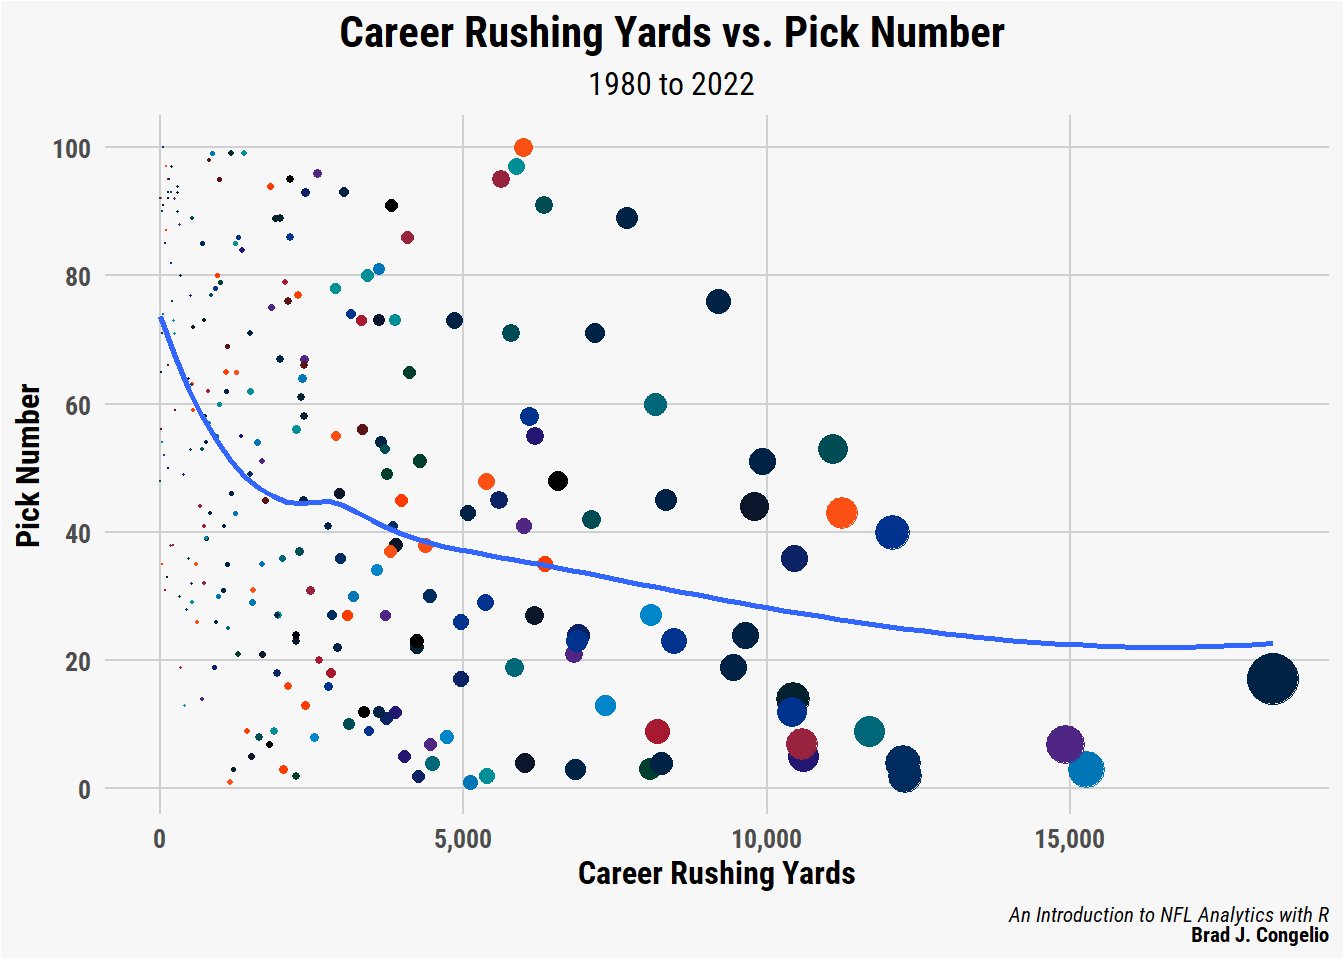
\includegraphics{03-nfl-analytics-functions_files/figure-pdf/running-back-plot-1.pdf}

}

\end{figure}

According to the plot, there has been a limited number of running backs
draft in the top 20 to go over 10,000 career yards. However, there are
more running backs - some still active - drafted in the mid-range of the
draft that are approaching, or have eclipsed, the 10,000 yard mark.

\hypertarget{the-load_combine-function}{%
\subsection{\texorpdfstring{The \texttt{load\_combine()}
Function}{The load\_combine() Function}}\label{the-load_combine-function}}

The \texttt{load\_combine()} function provides NFL Combine data dating
back to 2000. Aside from biographical information for each player
(including eventual draft position), the data include the player's
scores in the 40-yard dash, the bench press, the vertical, the broad
jump, the cone drill, and the shuttle drill.

We can join information from \texttt{load\_combine()} with outside
information to determine if there is any correlation between a running
back's 40-yard dash time in the combine and the total number of rushing
yard accumulated during his career.

\begin{Shaded}
\begin{Highlighting}[]
\NormalTok{combine\_data }\OtherTok{\textless{}{-}}\NormalTok{ nflreadr}\SpecialCharTok{::}\FunctionTok{load\_combine}\NormalTok{() }\SpecialCharTok{\%\textgreater{}\%}
  \FunctionTok{select}\NormalTok{(pfr\_id, forty) }\SpecialCharTok{\%\textgreater{}\%}
  \FunctionTok{filter}\NormalTok{(}\SpecialCharTok{!}\FunctionTok{is.na}\NormalTok{(pfr\_id) }\SpecialCharTok{\&} \SpecialCharTok{!}\FunctionTok{is.na}\NormalTok{(forty))}

\NormalTok{rosters }\OtherTok{\textless{}{-}}\NormalTok{ nflreadr}\SpecialCharTok{::}\FunctionTok{load\_rosters}\NormalTok{(}\DecValTok{2000}\SpecialCharTok{:}\DecValTok{2022}\NormalTok{) }\SpecialCharTok{\%\textgreater{}\%}
  \FunctionTok{select}\NormalTok{(gsis\_id, pfr\_id) }\SpecialCharTok{\%\textgreater{}\%}
  \FunctionTok{distinct}\NormalTok{(gsis\_id, }\AttributeTok{.keep\_all =} \ConstantTok{TRUE}\NormalTok{)}

\NormalTok{player\_stats }\OtherTok{\textless{}{-}}\NormalTok{ nflreadr}\SpecialCharTok{::}\FunctionTok{load\_player\_stats}\NormalTok{(}\AttributeTok{seasons =} \ConstantTok{TRUE}\NormalTok{,}
                                            \AttributeTok{stat\_type =} \StringTok{"offense"}\NormalTok{) }\SpecialCharTok{\%\textgreater{}\%}
  \FunctionTok{filter}\NormalTok{(position }\SpecialCharTok{==} \StringTok{"RB"} \SpecialCharTok{\&} \SpecialCharTok{!}\FunctionTok{is.na}\NormalTok{(player\_name) }\SpecialCharTok{\&}
\NormalTok{           season\_type }\SpecialCharTok{==} \StringTok{"REG"}\NormalTok{) }\SpecialCharTok{\%\textgreater{}\%}
  \FunctionTok{group\_by}\NormalTok{(player\_name, player\_id) }\SpecialCharTok{\%\textgreater{}\%}
  \FunctionTok{summarize}\NormalTok{(}\AttributeTok{total\_yards =} \FunctionTok{sum}\NormalTok{(rushing\_yards, }\AttributeTok{na.rm =} \ConstantTok{TRUE}\NormalTok{),}
            \AttributeTok{team =} \FunctionTok{last}\NormalTok{(recent\_team))}

\NormalTok{player\_stats }\OtherTok{\textless{}{-}}\NormalTok{ player\_stats }\SpecialCharTok{\%\textgreater{}\%}
  \FunctionTok{left\_join}\NormalTok{(rosters, }\AttributeTok{by =} \FunctionTok{c}\NormalTok{(}\StringTok{"player\_id"} \OtherTok{=} \StringTok{"gsis\_id"}\NormalTok{))}

\NormalTok{player\_stats }\OtherTok{\textless{}{-}}\NormalTok{ player\_stats }\SpecialCharTok{\%\textgreater{}\%}
  \FunctionTok{filter}\NormalTok{(}\SpecialCharTok{!}\FunctionTok{is.na}\NormalTok{(pfr\_id))}

\NormalTok{player\_stats }\OtherTok{\textless{}{-}}\NormalTok{ player\_stats }\SpecialCharTok{\%\textgreater{}\%}
  \FunctionTok{left\_join}\NormalTok{(combine\_data, }\AttributeTok{by =} \FunctionTok{c}\NormalTok{(}\StringTok{"pfr\_id"} \OtherTok{=} \StringTok{"pfr\_id"}\NormalTok{)) }\SpecialCharTok{\%\textgreater{}\%}
  \FunctionTok{filter}\NormalTok{(}\SpecialCharTok{!}\FunctionTok{is.na}\NormalTok{(forty))}

\NormalTok{player\_stats }\OtherTok{\textless{}{-}}\NormalTok{ player\_stats }\SpecialCharTok{\%\textgreater{}\%}
  \FunctionTok{left\_join}\NormalTok{(teams, }\AttributeTok{by =} \FunctionTok{c}\NormalTok{(}\StringTok{"team"} \OtherTok{=} \StringTok{"team\_abbr"}\NormalTok{))}
\end{Highlighting}
\end{Shaded}

\begin{Shaded}
\begin{Highlighting}[]
\FunctionTok{ggplot}\NormalTok{(}\AttributeTok{data =}\NormalTok{ player\_stats, }\FunctionTok{aes}\NormalTok{(}\AttributeTok{x =}\NormalTok{ forty, }\AttributeTok{y =}\NormalTok{ total\_yards)) }\SpecialCharTok{+}
  \FunctionTok{geom\_point}\NormalTok{(}\AttributeTok{color =}\NormalTok{ player\_stats}\SpecialCharTok{$}\NormalTok{team\_color, }\AttributeTok{size =} \FloatTok{3.5}\NormalTok{) }\SpecialCharTok{+}
  \FunctionTok{geom\_smooth}\NormalTok{(}\AttributeTok{method =}\NormalTok{ lm, }\AttributeTok{se =} \ConstantTok{FALSE}\NormalTok{,}
              \AttributeTok{color =} \StringTok{"black"}\NormalTok{,}
              \AttributeTok{linetype =} \StringTok{"dashed"}\NormalTok{,}
              \AttributeTok{size =} \FloatTok{0.8}\NormalTok{) }\SpecialCharTok{+}
  \FunctionTok{scale\_x\_continuous}\NormalTok{(}\AttributeTok{breaks =}\NormalTok{ scales}\SpecialCharTok{::}\FunctionTok{pretty\_breaks}\NormalTok{()) }\SpecialCharTok{+}
  \FunctionTok{scale\_y\_continuous}\NormalTok{(}\AttributeTok{breaks =}\NormalTok{ scales}\SpecialCharTok{::}\FunctionTok{pretty\_breaks}\NormalTok{(),}
                     \AttributeTok{labels =}\NormalTok{ scales}\SpecialCharTok{::}\FunctionTok{comma\_format}\NormalTok{()) }\SpecialCharTok{+}
  \FunctionTok{nfl\_analytics\_theme}\NormalTok{() }\SpecialCharTok{+}
  \FunctionTok{xlab}\NormalTok{(}\StringTok{"Forty{-}Yard Dash Time"}\NormalTok{) }\SpecialCharTok{+}
  \FunctionTok{ylab}\NormalTok{(}\StringTok{"Career Rushing Yards"}\NormalTok{) }\SpecialCharTok{+}
  \FunctionTok{labs}\NormalTok{(}\AttributeTok{title =} \StringTok{"**Forty{-}Yard Dash Time vs. Career Rushing Yards**"}\NormalTok{,}
       \AttributeTok{subtitle =} \StringTok{"2000 to 2022"}\NormalTok{,}
       \AttributeTok{caption =} \StringTok{"*An Introduction to NFL Analytics with R*\textless{}br\textgreater{}**Brad J. Congelio**"}\NormalTok{)}
\end{Highlighting}
\end{Shaded}

\begin{verbatim}
Warning: Using `size` aesthetic for lines was deprecated in ggplot2 3.4.0.
i Please use `linewidth` instead.
\end{verbatim}

\begin{verbatim}
`geom_smooth()` using formula = 'y ~ x'
\end{verbatim}

\begin{figure}[H]

{\centering 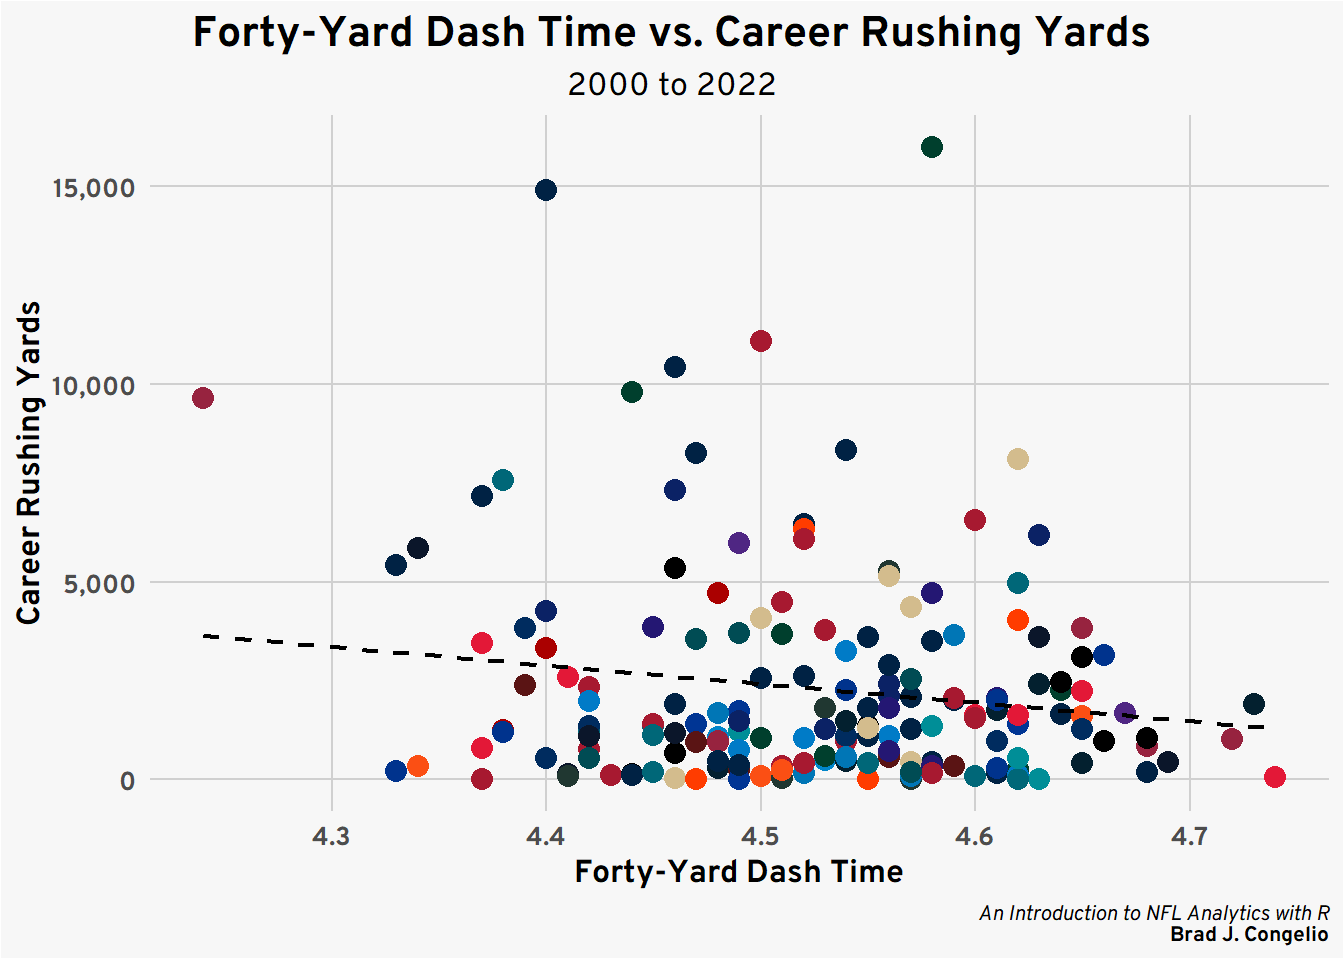
\includegraphics{03-nfl-analytics-functions_files/figure-pdf/running-back-40-plot-1.pdf}

}

\end{figure}

The visualization indicates that there is little, if any, direct
correlation between a running back's 40-yard dash time and his career
total rushing yards. There are likely other factors that contribute to
total rushing yards, such as a running back's agility and vision and -
perhaps most important - the quality of the offensive line over the
duration of the running back's career.

\hypertarget{the-load_nextgen_stats-function}{%
\subsection{\texorpdfstring{The \texttt{load\_nextgen\_stats()}
Function}{The load\_nextgen\_stats() Function}}\label{the-load_nextgen_stats-function}}

The \texttt{load\_nextgen\_stats()} function retrieves player-level
weekly statistics as provided by NFL Next Gen Stats dating back to the
2016 season. While three different stat types are provided (passing,
receiving, and rushing), it is important to note that the data will only
contain those players above a minimum number of attempts as determined
by the NFL Next Gen Stats team.

To illustrate what can be done with the \texttt{load\_nextgen\_stats()}
function, we will gather information to create two different plots.
First, we can plot each quarterback's average time to throw against
their average completed air yards. Second, we will construct a graph to
highlight which running backs had more actual rushing yards than the NGS
``expected rushing yards'' model.

\begin{Shaded}
\begin{Highlighting}[]
\NormalTok{ngs\_data\_passing }\OtherTok{\textless{}{-}}\NormalTok{ nflreadr}\SpecialCharTok{::}\FunctionTok{load\_nextgen\_stats}\NormalTok{(}\AttributeTok{seasons =} \DecValTok{2022}\NormalTok{,}
                                                 \AttributeTok{stat\_type =} \StringTok{"passing"}\NormalTok{) }\SpecialCharTok{\%\textgreater{}\%}
  \FunctionTok{filter}\NormalTok{(week }\SpecialCharTok{==} \DecValTok{0}\NormalTok{) }\SpecialCharTok{\%\textgreater{}\%}
  \FunctionTok{select}\NormalTok{(player\_display\_name, team\_abbr,}
\NormalTok{         avg\_time\_to\_throw, avg\_completed\_air\_yards)}

\NormalTok{ngs\_data\_passing }\OtherTok{\textless{}{-}}\NormalTok{ ngs\_data\_passing }\SpecialCharTok{\%\textgreater{}\%}
  \FunctionTok{left\_join}\NormalTok{(teams, }\AttributeTok{b =} \FunctionTok{c}\NormalTok{(}\StringTok{"team\_abbr"} \OtherTok{=} \StringTok{"team\_abbr"}\NormalTok{))}
\end{Highlighting}
\end{Shaded}

\begin{Shaded}
\begin{Highlighting}[]
\FunctionTok{ggplot}\NormalTok{(}\AttributeTok{data =}\NormalTok{ ngs\_data\_passing, }\FunctionTok{aes}\NormalTok{(}\AttributeTok{x =}\NormalTok{ avg\_time\_to\_throw,}
                                    \AttributeTok{y =}\NormalTok{ avg\_completed\_air\_yards)) }\SpecialCharTok{+}
  \FunctionTok{geom\_hline}\NormalTok{(}\AttributeTok{yintercept =} \FunctionTok{mean}\NormalTok{(ngs\_data\_passing}\SpecialCharTok{$}\NormalTok{avg\_completed\_air\_yards),}
             \AttributeTok{color =} \StringTok{"black"}\NormalTok{, }\AttributeTok{size =} \FloatTok{0.8}\NormalTok{, }\AttributeTok{linetype =} \StringTok{"dashed"}\NormalTok{) }\SpecialCharTok{+}
  \FunctionTok{geom\_vline}\NormalTok{(}\AttributeTok{xintercept =} \FunctionTok{mean}\NormalTok{(ngs\_data\_passing}\SpecialCharTok{$}\NormalTok{avg\_time\_to\_throw),}
             \AttributeTok{color =} \StringTok{"black"}\NormalTok{, }\AttributeTok{size =} \FloatTok{0.8}\NormalTok{, }\AttributeTok{linetype =} \StringTok{"dashed"}\NormalTok{) }\SpecialCharTok{+}
  \FunctionTok{geom\_point}\NormalTok{(}\AttributeTok{size =} \FloatTok{3.5}\NormalTok{, }\AttributeTok{color =}\NormalTok{ ngs\_data\_passing}\SpecialCharTok{$}\NormalTok{team\_color) }\SpecialCharTok{+}
  \FunctionTok{scale\_x\_continuous}\NormalTok{(}\AttributeTok{breaks =}\NormalTok{ scales}\SpecialCharTok{::}\FunctionTok{pretty\_breaks}\NormalTok{(),}
                     \AttributeTok{labels =}\NormalTok{ scales}\SpecialCharTok{::}\FunctionTok{comma\_format}\NormalTok{()) }\SpecialCharTok{+}
  \FunctionTok{scale\_y\_continuous}\NormalTok{(}\AttributeTok{breaks =}\NormalTok{ scales}\SpecialCharTok{::}\FunctionTok{pretty\_breaks}\NormalTok{(),}
                     \AttributeTok{labels =}\NormalTok{ scales}\SpecialCharTok{::}\FunctionTok{comma\_format}\NormalTok{()) }\SpecialCharTok{+}
  \FunctionTok{geom\_text\_repel}\NormalTok{(}\FunctionTok{aes}\NormalTok{(}\AttributeTok{label =}\NormalTok{ player\_display\_name),}
                  \AttributeTok{family =} \StringTok{"Roboto"}\NormalTok{, }\AttributeTok{fontface =} \StringTok{"bold"}\NormalTok{, }\AttributeTok{size =} \FloatTok{3.5}\NormalTok{) }\SpecialCharTok{+}
  \FunctionTok{nfl\_analytics\_theme}\NormalTok{() }\SpecialCharTok{+}
  \FunctionTok{xlab}\NormalTok{(}\StringTok{"Average Time to Throw"}\NormalTok{) }\SpecialCharTok{+}
  \FunctionTok{ylab}\NormalTok{(}\StringTok{"Average Completed Air Yards"}\NormalTok{) }\SpecialCharTok{+}
  \FunctionTok{labs}\NormalTok{(}\AttributeTok{title =} \StringTok{"**Avgerage Time to Throw vs. Average Air Yards**"}\NormalTok{,}
       \AttributeTok{subtitle =} \StringTok{"2022 Regular Season"}\NormalTok{,}
       \AttributeTok{caption =} \StringTok{"*An Introduction to NFL Analytics with R*\textless{}br\textgreater{}**Brad J. Congelio**"}\NormalTok{)}
\end{Highlighting}
\end{Shaded}

\begin{verbatim}
Warning: Removed 2 rows containing missing values (`geom_point()`).
\end{verbatim}

\begin{verbatim}
Warning: ggrepel: 8 unlabeled data points (too many overlaps). Consider
increasing max.overlaps
\end{verbatim}

\begin{figure}[H]

{\centering 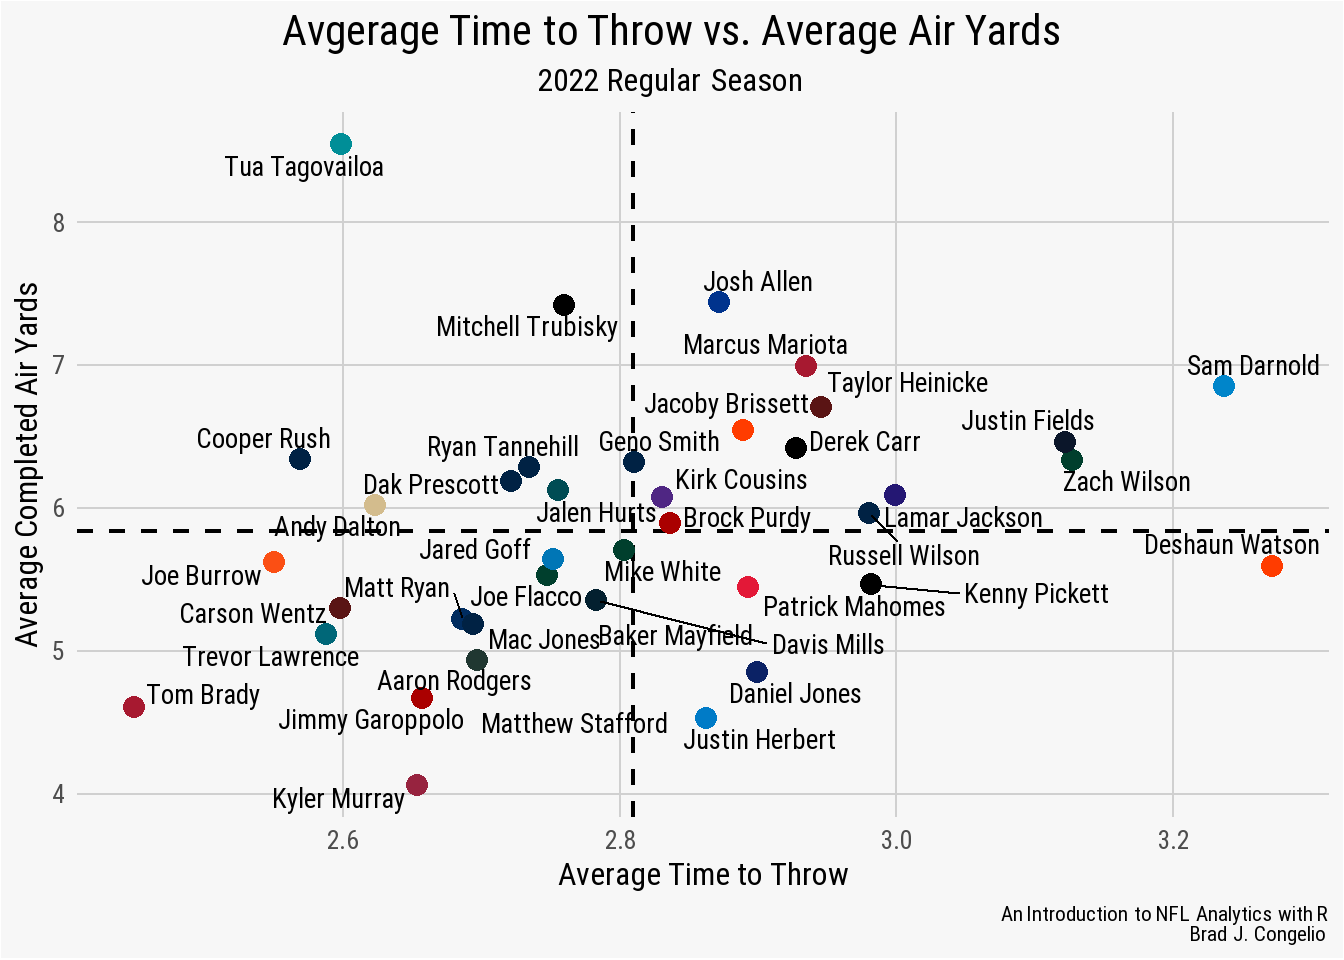
\includegraphics{03-nfl-analytics-functions_files/figure-pdf/ngs-passing-plot-1.pdf}

}

\end{figure}

The resulting plot shows that Dak Prescott, Jalen Hurts, and Ryan
Tannehill had an average completed air yard above the NFL average
despite getting rid of the ball quicker than most other quarterbacks in
the league. Conversely, Patrick Mahomes, Daniel Jones, and Justin
Herbert has under average completed air yards despite holding on to the
ball longer than the rest of the league (on average).

\begin{Shaded}
\begin{Highlighting}[]
\NormalTok{ngs\_data\_rushing }\OtherTok{\textless{}{-}}\NormalTok{ nflreadr}\SpecialCharTok{::}\FunctionTok{load\_nextgen\_stats}\NormalTok{(}\AttributeTok{seasons =} \DecValTok{2022}\NormalTok{,}
                                                 \AttributeTok{stat\_type =} \StringTok{"rushing"}\NormalTok{) }\SpecialCharTok{\%\textgreater{}\%}
  \FunctionTok{filter}\NormalTok{(week }\SpecialCharTok{==} \DecValTok{0}\NormalTok{) }\SpecialCharTok{\%\textgreater{}\%}
  \FunctionTok{select}\NormalTok{(player\_display\_name, team\_abbr, expected\_rush\_yards,}
\NormalTok{         rush\_yards\_over\_expected) }\SpecialCharTok{\%\textgreater{}\%}
  \FunctionTok{mutate}\NormalTok{(}\AttributeTok{actual\_rush\_yards =}\NormalTok{ expected\_rush\_yards }\SpecialCharTok{+}\NormalTok{ rush\_yards\_over\_expected)}

\NormalTok{ngs\_data\_rushing }\OtherTok{\textless{}{-}}\NormalTok{ ngs\_data\_rushing }\SpecialCharTok{\%\textgreater{}\%}
  \FunctionTok{left\_join}\NormalTok{(teams, }\AttributeTok{by =} \FunctionTok{c}\NormalTok{(}\StringTok{"team\_abbr"} \OtherTok{=} \StringTok{"team\_abbr"}\NormalTok{))}
\end{Highlighting}
\end{Shaded}

\begin{Shaded}
\begin{Highlighting}[]
\FunctionTok{ggplot}\NormalTok{(}\AttributeTok{data =}\NormalTok{ ngs\_data\_rushing, }\FunctionTok{aes}\NormalTok{(}\AttributeTok{x =}\NormalTok{ expected\_rush\_yards,}
                                    \AttributeTok{y =}\NormalTok{ actual\_rush\_yards)) }\SpecialCharTok{+}
  \FunctionTok{geom\_smooth}\NormalTok{(}\AttributeTok{method =}\NormalTok{ lm, }\AttributeTok{se =} \ConstantTok{FALSE}\NormalTok{,}
              \AttributeTok{color =} \StringTok{"black"}\NormalTok{,}
              \AttributeTok{size =} \FloatTok{0.8}\NormalTok{,}
              \AttributeTok{linetype =} \StringTok{"dashed"}\NormalTok{) }\SpecialCharTok{+}
  \FunctionTok{geom\_point}\NormalTok{(}\AttributeTok{size =} \FloatTok{3.5}\NormalTok{, }\AttributeTok{color =}\NormalTok{ ngs\_data\_rushing}\SpecialCharTok{$}\NormalTok{team\_color) }\SpecialCharTok{+}
  \FunctionTok{scale\_x\_continuous}\NormalTok{(}\AttributeTok{breaks =}\NormalTok{ scales}\SpecialCharTok{::}\FunctionTok{pretty\_breaks}\NormalTok{(),}
                     \AttributeTok{labels =}\NormalTok{ scales}\SpecialCharTok{::}\FunctionTok{comma\_format}\NormalTok{()) }\SpecialCharTok{+}
  \FunctionTok{scale\_y\_continuous}\NormalTok{(}\AttributeTok{breaks =}\NormalTok{ scales}\SpecialCharTok{::}\FunctionTok{pretty\_breaks}\NormalTok{(),}
                     \AttributeTok{labels =}\NormalTok{ scales}\SpecialCharTok{::}\FunctionTok{comma\_format}\NormalTok{()) }\SpecialCharTok{+}
  \FunctionTok{geom\_text\_repel}\NormalTok{(}\FunctionTok{aes}\NormalTok{(}\AttributeTok{label =}\NormalTok{ player\_display\_name),}
                  \AttributeTok{family =} \StringTok{"Roboto"}\NormalTok{,}
                  \AttributeTok{fontface =} \StringTok{"bold"}\NormalTok{, }\AttributeTok{size =} \FloatTok{3.5}\NormalTok{) }\SpecialCharTok{+}
  \FunctionTok{nfl\_analytics\_theme}\NormalTok{() }\SpecialCharTok{+}
  \FunctionTok{xlab}\NormalTok{(}\StringTok{"Expected Rush Yards"}\NormalTok{) }\SpecialCharTok{+}
  \FunctionTok{ylab}\NormalTok{(}\StringTok{"Actual Rush Yards"}\NormalTok{) }\SpecialCharTok{+}
  \FunctionTok{labs}\NormalTok{(}\AttributeTok{title =} \StringTok{"Expected Rush Yards vs. Actual Rush Yards"}\NormalTok{,}
       \AttributeTok{subtitle =} \StringTok{"2022 Regular Season"}\NormalTok{,}
       \AttributeTok{caption =} \StringTok{"*An Introduction to NFL Analytics with R*\textless{}br\textgreater{}**Brad J. Congelio**"}\NormalTok{)}
\end{Highlighting}
\end{Shaded}

\begin{verbatim}
`geom_smooth()` using formula = 'y ~ x'
\end{verbatim}

\begin{verbatim}
Warning: Removed 1 rows containing missing values (`geom_point()`).
\end{verbatim}

\begin{verbatim}
Warning: ggrepel: 38 unlabeled data points (too many overlaps). Consider
increasing max.overlaps
\end{verbatim}

\begin{figure}[H]

{\centering 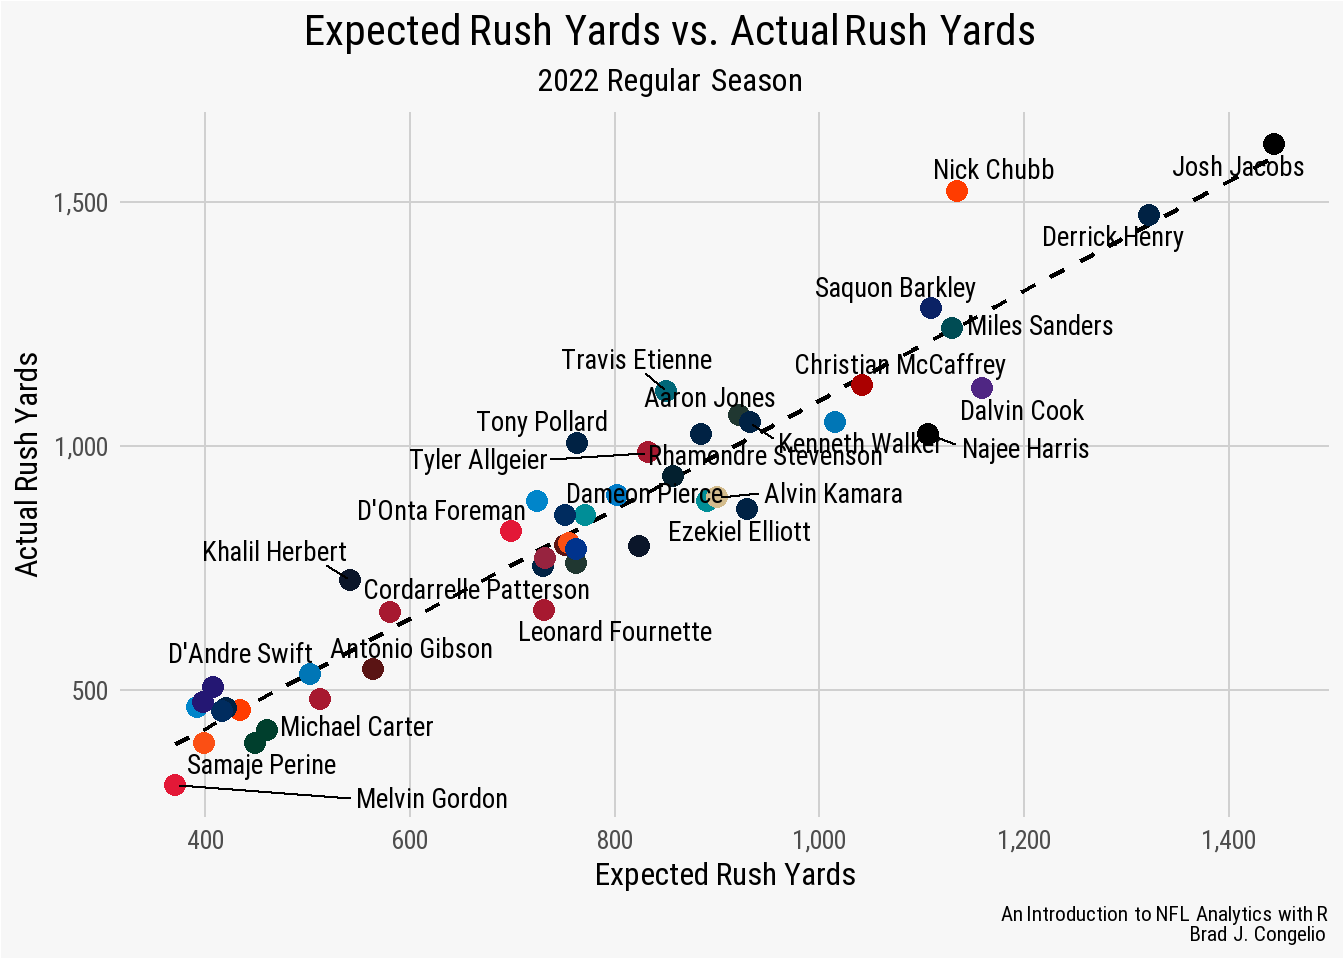
\includegraphics{03-nfl-analytics-functions_files/figure-pdf/ngs-rushing-plot-1.pdf}

}

\end{figure}

After plotting the rushing data from Next Gen Stats, we can see that
Nick Chubb was well above the expected yardage metric while Ezekiel
Elliott, Alvin Kamara, Najee Harris, and Dalvin Cook all had actual
rushing yards that fell below what was expected by the model.

\hypertarget{the-load_espn_qbr-function}{%
\subsection{\texorpdfstring{The \texttt{load\_espn\_qbr()}
Function}{The load\_espn\_qbr() Function}}\label{the-load_espn_qbr-function}}

With information dating back to the 2006 season, the
\texttt{load\_espn\_qbr()} function provides a multitude of data points,
including:

\begin{enumerate}
\def\labelenumi{\arabic{enumi}.}
\tightlist
\item
  \texttt{qbr\_total} - the adjusted total QBR which is calculated on a
  scale of 0-100 based on the strength of the defenses played.
\item
  \texttt{pts\_added} - the number of total points added by a
  quarterback adjusted above the average level of all other QBs.
\item
  \texttt{epa\_total} - the total number of expected points added for
  each quarterback as calculated by ESPN's win probability model.
\item
  \texttt{pass} - the total of expected points added for just pass
  plays.
\item
  \texttt{run} - the total of expected points added for just run plays.
\item
  \texttt{qbr\_raw} - the QBR without adjustment for strength of
  defense.
\item
  \texttt{sack} - the adjustment for expected points added for sacks.
\end{enumerate}

While the QBR metric has fallen out of grace among the analytics
community in recent years, we can still compare the difference between
the adjusted and unadjusted QBR scores to visualize the impact of
defensive strength on the total.

\begin{Shaded}
\begin{Highlighting}[]
\NormalTok{espn\_qbr }\OtherTok{\textless{}{-}}\NormalTok{ nflreadr}\SpecialCharTok{::}\FunctionTok{load\_espn\_qbr}\NormalTok{(}\AttributeTok{seasons =} \DecValTok{2022}\NormalTok{) }\SpecialCharTok{\%\textgreater{}\%}
  \FunctionTok{select}\NormalTok{(name\_short, team\_abb, qbr\_total, qbr\_raw)}

\NormalTok{espn\_qbr }\OtherTok{\textless{}{-}}\NormalTok{ espn\_qbr }\SpecialCharTok{\%\textgreater{}\%}
  \FunctionTok{left\_join}\NormalTok{(teams, }\AttributeTok{by =} \FunctionTok{c}\NormalTok{(}\StringTok{"team\_abb"} \OtherTok{=} \StringTok{"team\_abbr"}\NormalTok{))}
\end{Highlighting}
\end{Shaded}

\begin{Shaded}
\begin{Highlighting}[]
\FunctionTok{ggplot}\NormalTok{(}\AttributeTok{data =}\NormalTok{ espn\_qbr, }\FunctionTok{aes}\NormalTok{(}\AttributeTok{x =}\NormalTok{ qbr\_total, }\AttributeTok{y =}\NormalTok{ qbr\_raw)) }\SpecialCharTok{+}
  \FunctionTok{geom\_smooth}\NormalTok{(}\AttributeTok{method =}\NormalTok{ lm, }\AttributeTok{se =} \ConstantTok{FALSE}\NormalTok{,}
              \AttributeTok{color =} \StringTok{"black"}\NormalTok{,}
              \AttributeTok{linetype =} \StringTok{"dashed"}\NormalTok{,}
              \AttributeTok{size =} \FloatTok{0.8}\NormalTok{) }\SpecialCharTok{+}
  \FunctionTok{geom\_point}\NormalTok{(}\AttributeTok{color =}\NormalTok{ espn\_qbr}\SpecialCharTok{$}\NormalTok{team\_color, }\AttributeTok{size =} \FloatTok{3.5}\NormalTok{) }\SpecialCharTok{+}
  \FunctionTok{scale\_x\_continuous}\NormalTok{(}\AttributeTok{breaks =}\NormalTok{ scales}\SpecialCharTok{::}\FunctionTok{pretty\_breaks}\NormalTok{()) }\SpecialCharTok{+}
  \FunctionTok{scale\_y\_continuous}\NormalTok{(}\AttributeTok{breaks =}\NormalTok{ scales}\SpecialCharTok{::}\FunctionTok{pretty\_breaks}\NormalTok{()) }\SpecialCharTok{+}
  \FunctionTok{nfl\_analytics\_theme}\NormalTok{() }\SpecialCharTok{+}
  \FunctionTok{xlab}\NormalTok{(}\StringTok{"QBR {-} Adjusted"}\NormalTok{) }\SpecialCharTok{+}
  \FunctionTok{ylab}\NormalTok{(}\StringTok{"QBR {-} Unadjusted"}\NormalTok{) }\SpecialCharTok{+}
  \FunctionTok{labs}\NormalTok{(}\AttributeTok{title =} \StringTok{"QBR: Adjusted vs. Adjusted Scores"}\NormalTok{,}
       \AttributeTok{subtitle =} \StringTok{"Based on ESPN\textquotesingle{}s Model: 2022 Regular Season"}\NormalTok{,}
       \AttributeTok{caption =} \StringTok{"*An Introduction to NFL Analytics with R*\textless{}br\textgreater{}**Brad J. Congelio**"}\NormalTok{)}
\end{Highlighting}
\end{Shaded}

\begin{verbatim}
`geom_smooth()` using formula = 'y ~ x'
\end{verbatim}

\begin{verbatim}
Warning: Removed 4 rows containing missing values (`geom_point()`).
\end{verbatim}

\begin{figure}[H]

{\centering 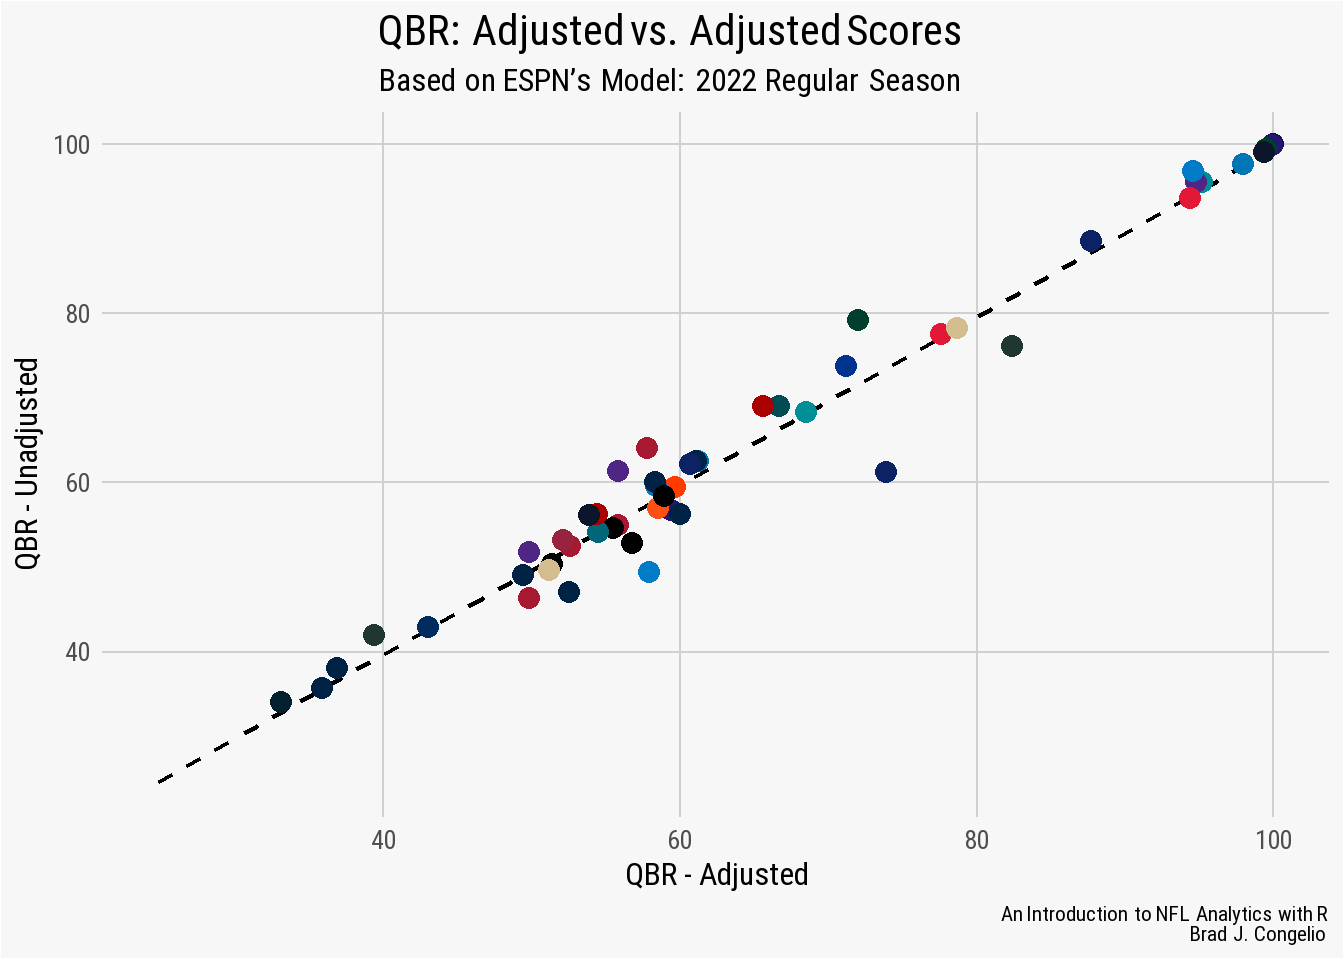
\includegraphics{03-nfl-analytics-functions_files/figure-pdf/qbr-adjusted-plot-1.pdf}

}

\end{figure}

\hypertarget{the-load_pfr_advstats-function}{%
\subsection{\texorpdfstring{The \texttt{load\_pfr\_advstats()}
Function}{The load\_pfr\_advstats() Function}}\label{the-load_pfr_advstats-function}}

The \texttt{load\_pfr\_advstats()} function provides statistics from Pro
Football Reference starting with the 2018 season for passing, rushing,
receiving, and defense. The function allows for collecting the data at
either the weekly or season level with the \texttt{summary\_level}
argument.

To begin exploring the data, let's examine the relationship between the
number of dropped passes each quarterback endured during the 2022
regular season compared to the total number of \texttt{bad\_throws}
charted by Pro Football Reference. An argument can be made that a
dropped pass without the pass being considered ``bad'' is the fault of
the wide receiver, while a dropped pass that \emph{is} charted as
``bad'' falls on the quarterback.

\begin{tcolorbox}[enhanced jigsaw, left=2mm, toprule=.15mm, opacitybacktitle=0.6, leftrule=.75mm, bottomrule=.15mm, colbacktitle=quarto-callout-important-color!10!white, breakable, colback=white, bottomtitle=1mm, toptitle=1mm, title=\textcolor{quarto-callout-important-color}{\faExclamation}\hspace{0.5em}{Important}, coltitle=black, titlerule=0mm, arc=.35mm, opacityback=0, colframe=quarto-callout-important-color-frame, rightrule=.15mm]

When working with data from \texttt{load\_pfr\_advstats()}, it is
important to remember that you must use the
\texttt{clean\_team\_abbrs()} function from \texttt{nflreadr} as there
is a difference between the abbreviations used by PFR and the
abbreviations used within the \texttt{nflverse}.

\end{tcolorbox}

\begin{Shaded}
\begin{Highlighting}[]
\NormalTok{pfr\_stats\_pass }\OtherTok{\textless{}{-}}\NormalTok{ nflreadr}\SpecialCharTok{::}\FunctionTok{load\_pfr\_advstats}\NormalTok{(}\AttributeTok{seasons =} \DecValTok{2022}\NormalTok{,}
                                              \AttributeTok{stat\_type =} \StringTok{"pass"}\NormalTok{,}
                                              \AttributeTok{summary\_level =} \StringTok{"season"}\NormalTok{) }\SpecialCharTok{\%\textgreater{}\%}
  \FunctionTok{select}\NormalTok{(player, pass\_attempts, team, drops, bad\_throws) }\SpecialCharTok{\%\textgreater{}\%}
  \FunctionTok{filter}\NormalTok{(pass\_attempts }\SpecialCharTok{\textgreater{}=} \DecValTok{400}\NormalTok{)}

\NormalTok{pfr\_stats\_pass}\SpecialCharTok{$}\NormalTok{team }\OtherTok{\textless{}{-}} \FunctionTok{clean\_team\_abbrs}\NormalTok{(pfr\_stats\_pass}\SpecialCharTok{$}\NormalTok{team)}

\NormalTok{pfr\_stats\_pass }\OtherTok{\textless{}{-}}\NormalTok{ pfr\_stats\_pass }\SpecialCharTok{\%\textgreater{}\%}
  \FunctionTok{left\_join}\NormalTok{(teams, }\AttributeTok{by =} \FunctionTok{c}\NormalTok{(}\StringTok{"team"} \OtherTok{=} \StringTok{"team\_abbr"}\NormalTok{))}
\end{Highlighting}
\end{Shaded}

\begin{Shaded}
\begin{Highlighting}[]
\FunctionTok{ggplot}\NormalTok{(}\AttributeTok{data =}\NormalTok{ pfr\_stats\_pass, }\FunctionTok{aes}\NormalTok{(}\AttributeTok{x =}\NormalTok{ bad\_throws, }\AttributeTok{y =}\NormalTok{ drops)) }\SpecialCharTok{+}
  \FunctionTok{geom\_hline}\NormalTok{(}\AttributeTok{yintercept =} \FunctionTok{mean}\NormalTok{(pfr\_stats\_pass}\SpecialCharTok{$}\NormalTok{drops),}
             \AttributeTok{color =} \StringTok{"black"}\NormalTok{, }\AttributeTok{linetype =} \StringTok{"dashed"}\NormalTok{, }\AttributeTok{size =} \FloatTok{0.8}\NormalTok{) }\SpecialCharTok{+}
  \FunctionTok{geom\_vline}\NormalTok{(}\AttributeTok{xintercept =} \FunctionTok{mean}\NormalTok{(pfr\_stats\_pass}\SpecialCharTok{$}\NormalTok{bad\_throws),}
             \AttributeTok{color =} \StringTok{"black"}\NormalTok{, }\AttributeTok{linetype =} \StringTok{"dashed"}\NormalTok{, }\AttributeTok{size =} \FloatTok{0.8}\NormalTok{) }\SpecialCharTok{+}
  \FunctionTok{geom\_point}\NormalTok{(}\AttributeTok{color =}\NormalTok{ pfr\_stats\_pass}\SpecialCharTok{$}\NormalTok{team\_color, }\AttributeTok{size =} \FloatTok{3.5}\NormalTok{) }\SpecialCharTok{+}
  \FunctionTok{scale\_x\_continuous}\NormalTok{(}\AttributeTok{breaks =}\NormalTok{ scales}\SpecialCharTok{::}\FunctionTok{pretty\_breaks}\NormalTok{()) }\SpecialCharTok{+}
  \FunctionTok{scale\_y\_continuous}\NormalTok{(}\AttributeTok{breaks =}\NormalTok{ scales}\SpecialCharTok{::}\FunctionTok{pretty\_breaks}\NormalTok{()) }\SpecialCharTok{+}
  \FunctionTok{nfl\_analytics\_theme}\NormalTok{() }\SpecialCharTok{+}
  \FunctionTok{geom\_text\_repel}\NormalTok{(}\FunctionTok{aes}\NormalTok{(}\AttributeTok{label =}\NormalTok{ player),}
                  \AttributeTok{family =} \StringTok{"Roboto"}\NormalTok{, }\AttributeTok{fontface =} \StringTok{"bold"}\NormalTok{, }\AttributeTok{size =} \FloatTok{3.5}\NormalTok{) }\SpecialCharTok{+}
  \FunctionTok{xlab}\NormalTok{(}\StringTok{"Bad Throws"}\NormalTok{) }\SpecialCharTok{+}
  \FunctionTok{ylab}\NormalTok{(}\StringTok{"Drops"}\NormalTok{) }\SpecialCharTok{+}
  \FunctionTok{labs}\NormalTok{(}\AttributeTok{title =} \StringTok{"**QB Bad Throws vs. WR Drops**"}\NormalTok{,}
       \AttributeTok{subtitle =} \StringTok{"2022 Regular Season"}\NormalTok{,}
       \AttributeTok{caption =} \StringTok{"*An Introduction to NFL Analytics with R*\textless{}br\textgreater{}**Brad J. Congelio**"}\NormalTok{)}
\end{Highlighting}
\end{Shaded}

\begin{figure}[H]

{\centering 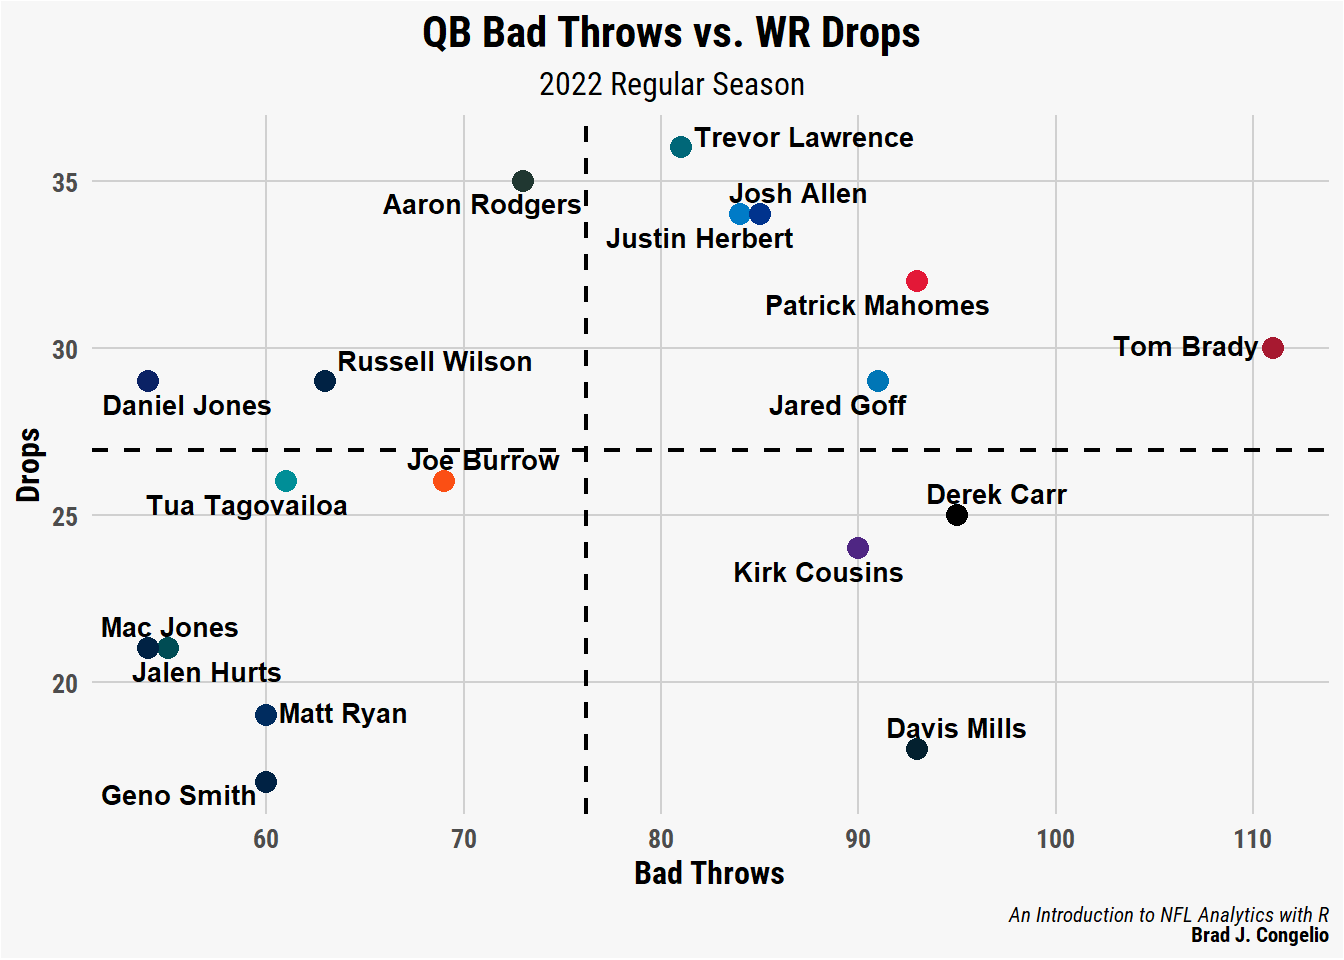
\includegraphics{03-nfl-analytics-functions_files/figure-pdf/qb-pfr-stats-plot-1.pdf}

}

\end{figure}

Quarterbacks such as Patrick Mahomes, Josh Allen, and Tom Brady had some
of the highest drop numbers in the league but were also charted as
having the highest number of bad throws, as well. This indicates that -
without additional context - the wide receivers may not be as much at
fault for the drops compared to the wide receivers that dropped passes
from Daniel Jones and Russell Wilson, both of whom had a lower number of
bad throws.

By using the rushing data provided by \texttt{load\_pfr\_advstats()}, we
can examine how ``hard'' it is to tackle a running back by examining the
relationship between their yards before contact and yards after contact.

\begin{tcolorbox}[enhanced jigsaw, left=2mm, toprule=.15mm, opacitybacktitle=0.6, leftrule=.75mm, bottomrule=.15mm, colbacktitle=quarto-callout-important-color!10!white, breakable, colback=white, bottomtitle=1mm, toptitle=1mm, title=\textcolor{quarto-callout-important-color}{\faExclamation}\hspace{0.5em}{Important}, coltitle=black, titlerule=0mm, arc=.35mm, opacityback=0, colframe=quarto-callout-important-color-frame, rightrule=.15mm]

Because the list of running backs with more than 200 attempts includes
Christian McCaffrey, it is necessary to use the \texttt{case\_when()}
function to switch his \texttt{tm} from \texttt{2TMS} to the team that
he finished the season with (\texttt{SF}). Otherwise, using
\texttt{left\_join()} for team colors would not work for McCafffrey
since \texttt{2TMS} is not a recognized team abbreviation.

\end{tcolorbox}

\begin{Shaded}
\begin{Highlighting}[]
\NormalTok{pfr\_stats\_rush }\OtherTok{\textless{}{-}}\NormalTok{ nflreadr}\SpecialCharTok{::}\FunctionTok{load\_pfr\_advstats}\NormalTok{(}\AttributeTok{seasons =} \DecValTok{2022}\NormalTok{,}
                                              \AttributeTok{stat\_type =} \StringTok{"rush"}\NormalTok{,}
                                              \AttributeTok{summary\_level =} \StringTok{"season"}\NormalTok{) }\SpecialCharTok{\%\textgreater{}\%}
  \FunctionTok{select}\NormalTok{(player, tm, att, ybc, yac) }\SpecialCharTok{\%\textgreater{}\%}
  \FunctionTok{filter}\NormalTok{(att }\SpecialCharTok{\textgreater{}=} \DecValTok{200}\NormalTok{) }\SpecialCharTok{\%\textgreater{}\%}
  \FunctionTok{mutate}\NormalTok{(}\AttributeTok{tm =} \FunctionTok{case\_when}\NormalTok{(}
\NormalTok{    player }\SpecialCharTok{==} \StringTok{"Christian McCaffrey"} \SpecialCharTok{\textasciitilde{}} \StringTok{"SF"}\NormalTok{,}
    \ConstantTok{TRUE} \SpecialCharTok{\textasciitilde{}}\NormalTok{ tm))}

\NormalTok{pfr\_stats\_rush}\SpecialCharTok{$}\NormalTok{tm }\OtherTok{\textless{}{-}} \FunctionTok{clean\_team\_abbrs}\NormalTok{(pfr\_stats\_rush}\SpecialCharTok{$}\NormalTok{tm)}

\NormalTok{pfr\_stats\_rush }\OtherTok{\textless{}{-}}\NormalTok{ pfr\_stats\_rush }\SpecialCharTok{\%\textgreater{}\%}
  \FunctionTok{left\_join}\NormalTok{(teams, }\AttributeTok{by =} \FunctionTok{c}\NormalTok{(}\StringTok{"tm"} \OtherTok{=} \StringTok{"team\_abbr"}\NormalTok{))}
\end{Highlighting}
\end{Shaded}

\begin{Shaded}
\begin{Highlighting}[]
\FunctionTok{ggplot}\NormalTok{(}\AttributeTok{data =}\NormalTok{ pfr\_stats\_rush, }\FunctionTok{aes}\NormalTok{(}\AttributeTok{x =}\NormalTok{ ybc, }\AttributeTok{y =}\NormalTok{ yac)) }\SpecialCharTok{+}
  \FunctionTok{geom\_hline}\NormalTok{(}\AttributeTok{yintercept =} \FunctionTok{mean}\NormalTok{(pfr\_stats\_rush}\SpecialCharTok{$}\NormalTok{yac),}
             \AttributeTok{color =} \StringTok{"black"}\NormalTok{, }\AttributeTok{linetype =} \StringTok{"dashed"}\NormalTok{, }\AttributeTok{size =} \FloatTok{0.8}\NormalTok{) }\SpecialCharTok{+}
  \FunctionTok{geom\_vline}\NormalTok{(}\AttributeTok{xintercept =} \FunctionTok{mean}\NormalTok{(pfr\_stats\_rush}\SpecialCharTok{$}\NormalTok{ybc),}
             \AttributeTok{color =} \StringTok{"black"}\NormalTok{, }\AttributeTok{linetype =} \StringTok{"dashed"}\NormalTok{, }\AttributeTok{size =} \FloatTok{0.8}\NormalTok{) }\SpecialCharTok{+}
  \FunctionTok{geom\_point}\NormalTok{(}\AttributeTok{color =}\NormalTok{ pfr\_stats\_rush}\SpecialCharTok{$}\NormalTok{team\_color, }\AttributeTok{size =} \FloatTok{3.5}\NormalTok{) }\SpecialCharTok{+}
  \FunctionTok{scale\_x\_continuous}\NormalTok{(}\AttributeTok{breaks =}\NormalTok{ scales}\SpecialCharTok{::}\FunctionTok{pretty\_breaks}\NormalTok{()) }\SpecialCharTok{+}
  \FunctionTok{scale\_y\_continuous}\NormalTok{(}\AttributeTok{breaks =}\NormalTok{ scales}\SpecialCharTok{::}\FunctionTok{pretty\_breaks}\NormalTok{()) }\SpecialCharTok{+}
  \FunctionTok{nfl\_analytics\_theme}\NormalTok{() }\SpecialCharTok{+}
  \FunctionTok{geom\_text\_repel}\NormalTok{(}\FunctionTok{aes}\NormalTok{(}\AttributeTok{label =}\NormalTok{ player),}
                  \AttributeTok{family =} \StringTok{"Roboto"}\NormalTok{, }\AttributeTok{fontface =} \StringTok{"bold"}\NormalTok{, }\AttributeTok{size =} \FloatTok{3.5}\NormalTok{) }\SpecialCharTok{+}
  \FunctionTok{xlab}\NormalTok{(}\StringTok{"Yards Before Contact"}\NormalTok{) }\SpecialCharTok{+}
  \FunctionTok{ylab}\NormalTok{(}\StringTok{"Yards After Contact"}\NormalTok{) }\SpecialCharTok{+}
  \FunctionTok{labs}\NormalTok{(}\AttributeTok{title =} \StringTok{"**Running Backs: Yards Before and After Contact**"}\NormalTok{,}
       \AttributeTok{subtitle =} \StringTok{"2022 Regular Season"}\NormalTok{,}
       \AttributeTok{caption =} \StringTok{"*An Introduction to NFL Analytics with R*\textless{}br\textgreater{}**Brad J. Congelio**"}\NormalTok{)}
\end{Highlighting}
\end{Shaded}

\begin{figure}[H]

{\centering 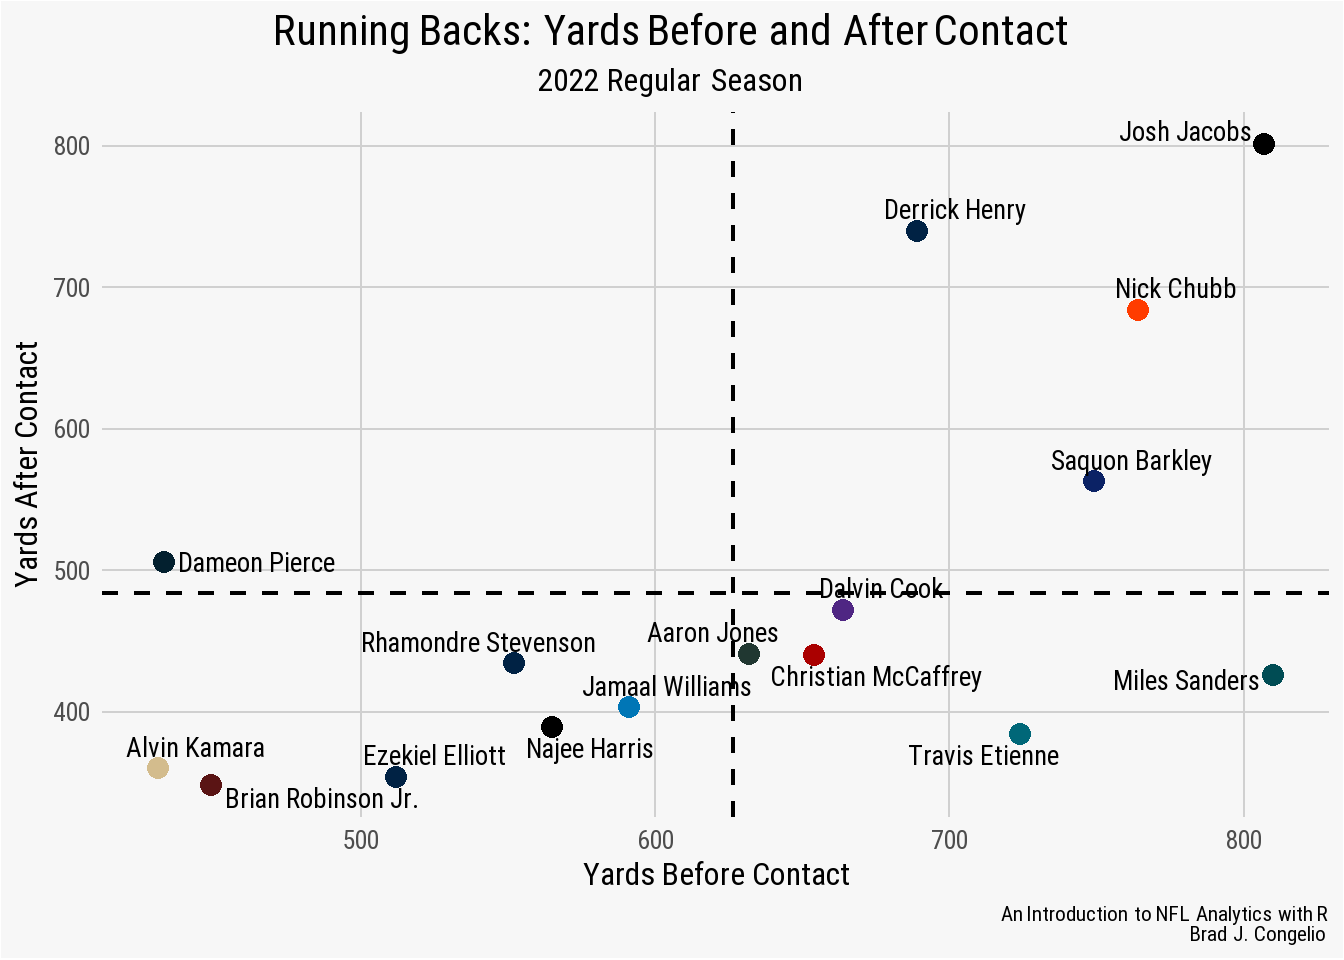
\includegraphics{03-nfl-analytics-functions_files/figure-pdf/pfr-rush-stats-plot-1.pdf}

}

\end{figure}

In the same vein as the running back statistics, we can use
\texttt{load\_pfr\_advstats()} to explore which wide receivers gained
the most yardage after catching the ball.

\begin{Shaded}
\begin{Highlighting}[]
\NormalTok{pfr\_stats\_rec }\OtherTok{\textless{}{-}}\NormalTok{ nflreadr}\SpecialCharTok{::}\FunctionTok{load\_pfr\_advstats}\NormalTok{(}\AttributeTok{seasons =} \DecValTok{2022}\NormalTok{, }\AttributeTok{stat\_type =} \StringTok{"rec"}\NormalTok{,}
                                             \AttributeTok{summary\_level =} \StringTok{"season"}\NormalTok{) }\SpecialCharTok{\%\textgreater{}\%}
  \FunctionTok{filter}\NormalTok{(rec }\SpecialCharTok{\textgreater{}=} \DecValTok{80} \SpecialCharTok{\&}\NormalTok{ pos }\SpecialCharTok{==} \StringTok{"WR"}\NormalTok{) }\SpecialCharTok{\%\textgreater{}\%}
  \FunctionTok{select}\NormalTok{(player, tm, rec, ybc, yac)}

\NormalTok{pfr\_stats\_rec }\OtherTok{\textless{}{-}}\NormalTok{ pfr\_stats\_rec }\SpecialCharTok{\%\textgreater{}\%}
  \FunctionTok{left\_join}\NormalTok{(teams, }\AttributeTok{by =} \FunctionTok{c}\NormalTok{(}\StringTok{"tm"} \OtherTok{=} \StringTok{"team\_abbr"}\NormalTok{))}
\end{Highlighting}
\end{Shaded}

\begin{Shaded}
\begin{Highlighting}[]
\FunctionTok{ggplot}\NormalTok{(}\AttributeTok{data =}\NormalTok{ pfr\_stats\_rec, }\FunctionTok{aes}\NormalTok{(}\AttributeTok{x =}\NormalTok{ ybc, }\AttributeTok{y =}\NormalTok{ yac)) }\SpecialCharTok{+}
  \FunctionTok{geom\_hline}\NormalTok{(}\AttributeTok{yintercept =} \FunctionTok{mean}\NormalTok{(pfr\_stats\_rec}\SpecialCharTok{$}\NormalTok{yac),}
             \AttributeTok{color =} \StringTok{"black"}\NormalTok{, }\AttributeTok{linetype =} \StringTok{"dashed"}\NormalTok{, }\AttributeTok{size =} \FloatTok{0.8}\NormalTok{) }\SpecialCharTok{+}
  \FunctionTok{geom\_vline}\NormalTok{(}\AttributeTok{xintercept =} \FunctionTok{mean}\NormalTok{(pfr\_stats\_rec}\SpecialCharTok{$}\NormalTok{ybc),}
             \AttributeTok{color =} \StringTok{"black"}\NormalTok{, }\AttributeTok{linetype =} \StringTok{"dashed"}\NormalTok{, }\AttributeTok{size =} \FloatTok{0.8}\NormalTok{) }\SpecialCharTok{+}
  \FunctionTok{geom\_point}\NormalTok{(}\AttributeTok{color =}\NormalTok{ pfr\_stats\_rec}\SpecialCharTok{$}\NormalTok{team\_color, }\AttributeTok{size =} \FloatTok{3.5}\NormalTok{) }\SpecialCharTok{+}
  \FunctionTok{scale\_x\_continuous}\NormalTok{(}\AttributeTok{breaks =}\NormalTok{ scales}\SpecialCharTok{::}\FunctionTok{pretty\_breaks}\NormalTok{(),}
                     \AttributeTok{labels =}\NormalTok{ scales}\SpecialCharTok{::}\FunctionTok{comma\_format}\NormalTok{()) }\SpecialCharTok{+}
  \FunctionTok{scale\_y\_continuous}\NormalTok{(}\AttributeTok{breaks =}\NormalTok{ scales}\SpecialCharTok{::}\FunctionTok{pretty\_breaks}\NormalTok{()) }\SpecialCharTok{+}
  \FunctionTok{nfl\_analytics\_theme}\NormalTok{() }\SpecialCharTok{+}
  \FunctionTok{geom\_text\_repel}\NormalTok{(}\FunctionTok{aes}\NormalTok{(}\AttributeTok{label =}\NormalTok{ player),}
                  \AttributeTok{family =} \StringTok{"Roboto"}\NormalTok{, }\AttributeTok{fontface =} \StringTok{"bold"}\NormalTok{, }\AttributeTok{size =} \FloatTok{3.5}\NormalTok{) }\SpecialCharTok{+}
  \FunctionTok{xlab}\NormalTok{(}\StringTok{"Yards At Point of Catch"}\NormalTok{) }\SpecialCharTok{+}
  \FunctionTok{ylab}\NormalTok{(}\StringTok{"Yards After Catch"}\NormalTok{) }\SpecialCharTok{+}
  \FunctionTok{labs}\NormalTok{(}\AttributeTok{title =} \StringTok{"**Yards at Point of Catch vs. Yards After Catch"}\NormalTok{,}
       \AttributeTok{subtitle =} \StringTok{"2022 Regular Season"}\NormalTok{,}
       \AttributeTok{caption =} \StringTok{"*An Introduction to NFl Analytics with R*\textless{}br\textgreater{}**Brad J. Congelio**"}\NormalTok{)}
\end{Highlighting}
\end{Shaded}

\begin{figure}[H]

{\centering 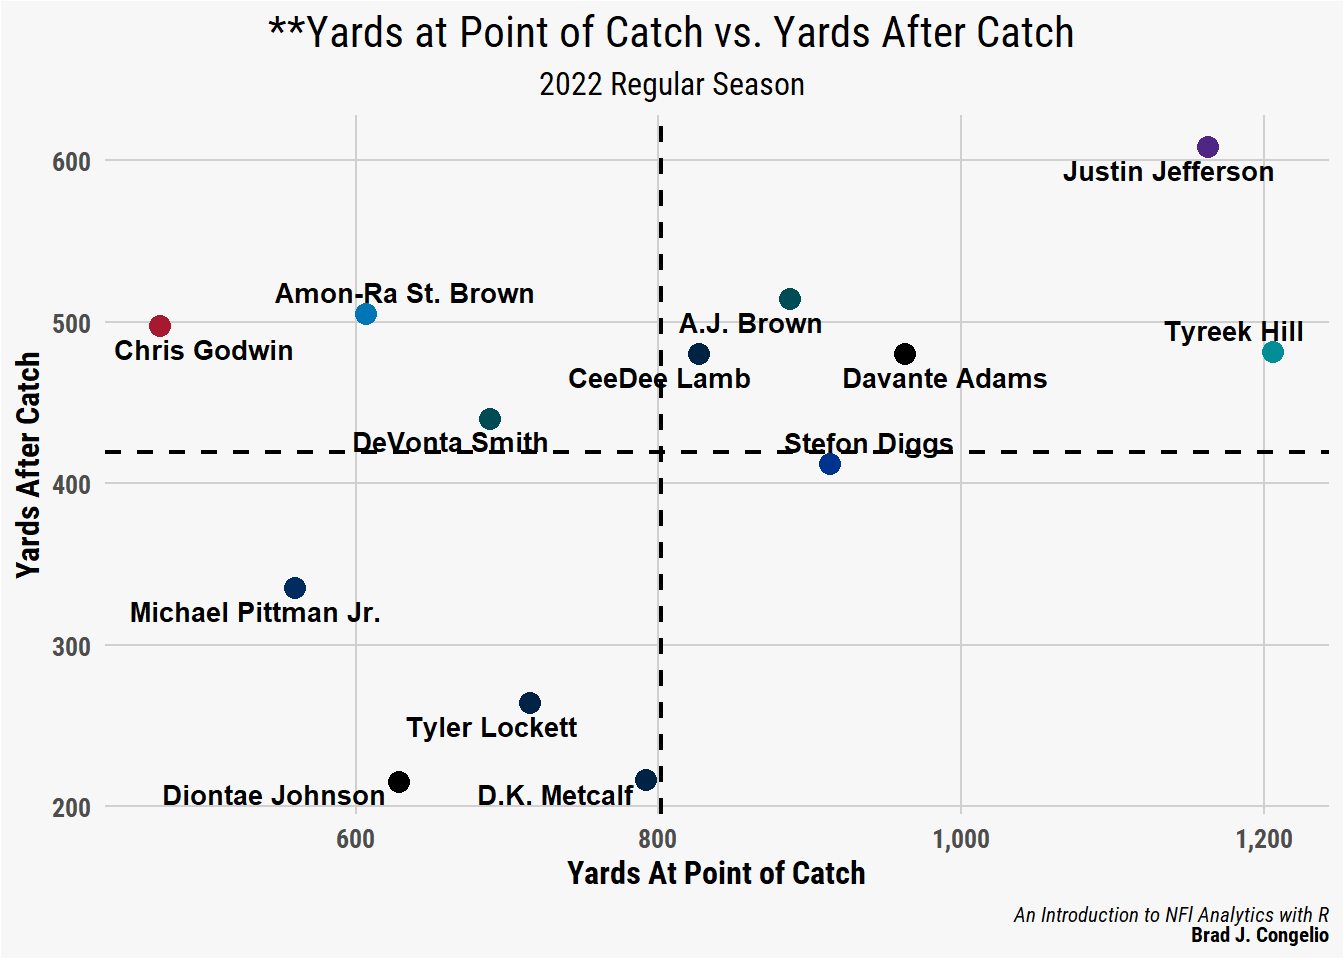
\includegraphics{03-nfl-analytics-functions_files/figure-pdf/pfr-rec-stats-plot-1.pdf}

}

\end{figure}

Given the outstanding season that Justin Jefferson had in 2022, it is
unsurprising to see him in the upper-right quadrant of the plot. Of his
1,809 receiving yards in the season, just under 1,200 of them came
through air yards while he gained just over an additional 600 yards on
the ground after the catch. On the other hand, D.K. Metcalf and Diontae
Johnson were more often than not tackled almost immediately after
catching the football.

Given the structure of the data collected from
\texttt{load\_pfr\_advstats()}, the information can also be aggregated
to define team total. For example, we can use the defensive statistics
for blitzes and sacks from individual players to calculate the
relationship between a team's total number of blitzes against the number
of sacks those blitzes produce.

\begin{Shaded}
\begin{Highlighting}[]
\NormalTok{pfr\_stats\_def }\OtherTok{\textless{}{-}}\NormalTok{ nflreadr}\SpecialCharTok{::}\FunctionTok{load\_pfr\_advstats}\NormalTok{(}\AttributeTok{seasons =} \DecValTok{2022}\NormalTok{,}
                                             \AttributeTok{stat\_type =} \StringTok{"def"}\NormalTok{,}
                                             \AttributeTok{summary\_level =} \StringTok{"season"}\NormalTok{) }\SpecialCharTok{\%\textgreater{}\%}
  \FunctionTok{filter}\NormalTok{(}\SpecialCharTok{!}\NormalTok{tm }\SpecialCharTok{\%in\%} \FunctionTok{c}\NormalTok{(}\StringTok{"2TM"}\NormalTok{, }\StringTok{"3TM"}\NormalTok{)) }\SpecialCharTok{\%\textgreater{}\%}
  \FunctionTok{select}\NormalTok{(tm, bltz, sk) }\SpecialCharTok{\%\textgreater{}\%}
  \FunctionTok{group\_by}\NormalTok{(tm) }\SpecialCharTok{\%\textgreater{}\%}
  \FunctionTok{summarize}\NormalTok{(}\AttributeTok{total\_blitz =} \FunctionTok{sum}\NormalTok{(bltz, }\AttributeTok{na.rm =} \ConstantTok{TRUE}\NormalTok{),}
            \AttributeTok{total\_sack =} \FunctionTok{sum}\NormalTok{(sk, }\AttributeTok{na.rm =} \ConstantTok{TRUE}\NormalTok{))}

\NormalTok{pfr\_stats\_def }\OtherTok{\textless{}{-}}\NormalTok{ pfr\_stats\_def }\SpecialCharTok{\%\textgreater{}\%}
  \FunctionTok{left\_join}\NormalTok{(teams, }\AttributeTok{by =} \FunctionTok{c}\NormalTok{(}\StringTok{"tm"} \OtherTok{=} \StringTok{"team\_abbr"}\NormalTok{))}
\end{Highlighting}
\end{Shaded}

\begin{Shaded}
\begin{Highlighting}[]
\FunctionTok{ggplot}\NormalTok{(}\AttributeTok{data =}\NormalTok{ pfr\_stats\_def, }\FunctionTok{aes}\NormalTok{(}\AttributeTok{x =}\NormalTok{ total\_blitz, }\AttributeTok{y =}\NormalTok{ total\_sack)) }\SpecialCharTok{+}
  \FunctionTok{geom\_hline}\NormalTok{(}\AttributeTok{yintercept =} \FunctionTok{mean}\NormalTok{(pfr\_stats\_def}\SpecialCharTok{$}\NormalTok{total\_sack),}
             \AttributeTok{color =} \StringTok{"black"}\NormalTok{, }\AttributeTok{linetype =} \StringTok{"dashed"}\NormalTok{, }\AttributeTok{size =} \FloatTok{0.8}\NormalTok{) }\SpecialCharTok{+}
  \FunctionTok{geom\_vline}\NormalTok{(}\AttributeTok{xintercept =} \FunctionTok{mean}\NormalTok{(pfr\_stats\_def}\SpecialCharTok{$}\NormalTok{total\_blitz),}
             \AttributeTok{color =} \StringTok{"black"}\NormalTok{, }\AttributeTok{linetype =} \StringTok{"dashed"}\NormalTok{, }\AttributeTok{size =} \FloatTok{0.8}\NormalTok{) }\SpecialCharTok{+}
  \FunctionTok{geom\_image}\NormalTok{(}\FunctionTok{aes}\NormalTok{(}\AttributeTok{image =}\NormalTok{ team\_logo\_wikipedia), }\AttributeTok{asp =} \DecValTok{16}\SpecialCharTok{/}\DecValTok{9}\NormalTok{) }\SpecialCharTok{+}
  \FunctionTok{scale\_x\_continuous}\NormalTok{(}\AttributeTok{breaks =}\NormalTok{ scales}\SpecialCharTok{::}\FunctionTok{pretty\_breaks}\NormalTok{()) }\SpecialCharTok{+}
  \FunctionTok{scale\_y\_continuous}\NormalTok{(}\AttributeTok{breaks =}\NormalTok{ scales}\SpecialCharTok{::}\FunctionTok{pretty\_breaks}\NormalTok{()) }\SpecialCharTok{+}
  \FunctionTok{nfl\_analytics\_theme}\NormalTok{() }\SpecialCharTok{+}
  \FunctionTok{xlab}\NormalTok{(}\StringTok{"Total Blitzes"}\NormalTok{) }\SpecialCharTok{+}
  \FunctionTok{ylab}\NormalTok{(}\StringTok{"Total Sacks"}\NormalTok{) }\SpecialCharTok{+}
  \FunctionTok{labs}\NormalTok{(}\AttributeTok{title =} \StringTok{"**Total Blitzes vs. Total Sacks**"}\NormalTok{,}
       \AttributeTok{subtitle =} \StringTok{"2022 Regular Season"}\NormalTok{,}
       \AttributeTok{caption =} \StringTok{"*An Introduction to NFL Analytics with R*\textless{}br\textgreater{}**Brad J. Congelio**"}\NormalTok{)}
\end{Highlighting}
\end{Shaded}

\begin{figure}[H]

{\centering 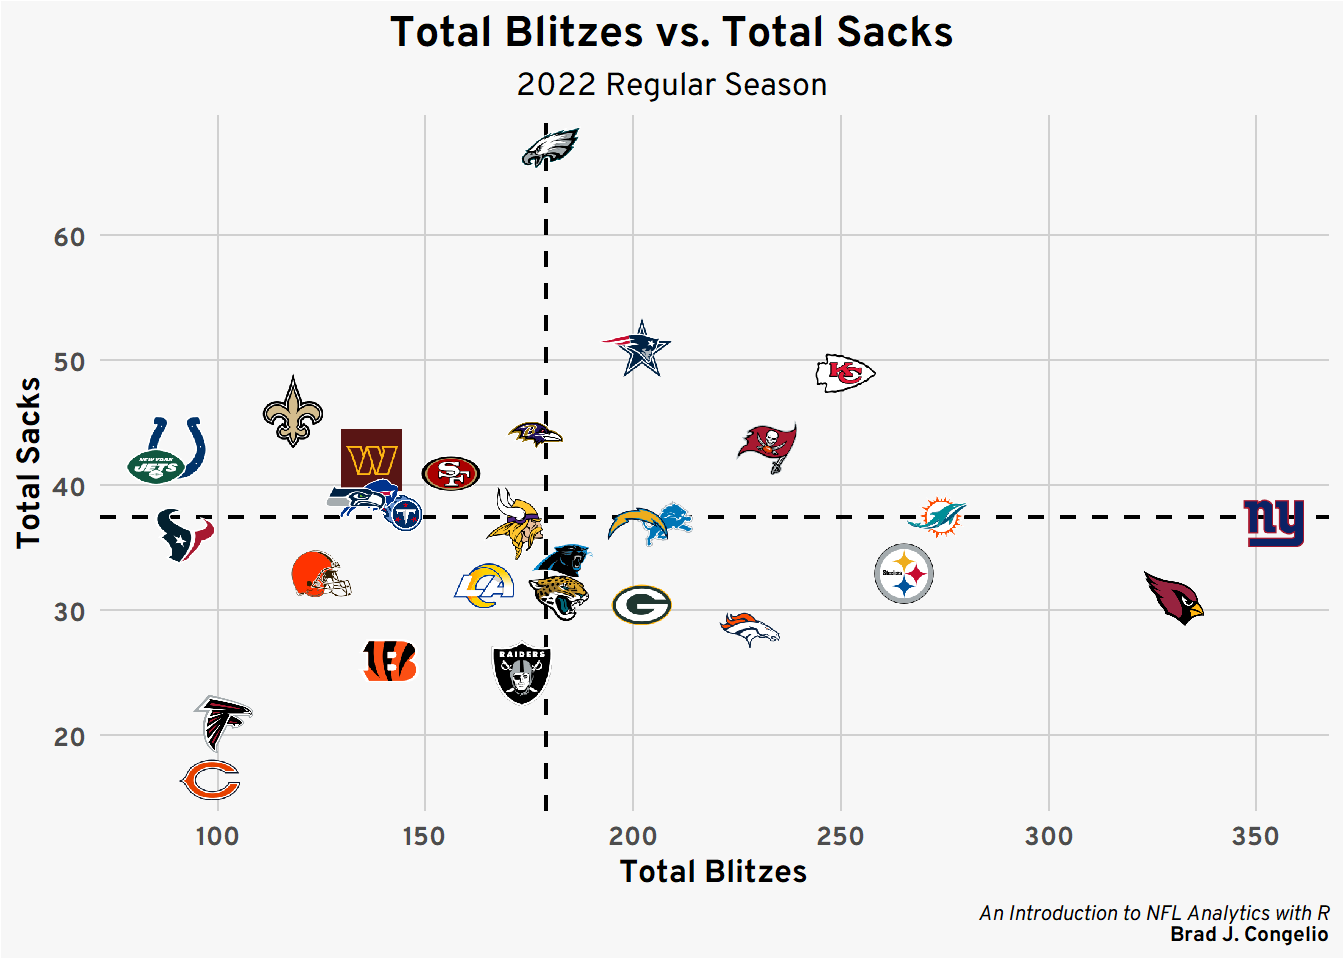
\includegraphics{03-nfl-analytics-functions_files/figure-pdf/blitz-sacks-plot-1.pdf}

}

\end{figure}

The Philadelphia Eagles were absolutely dominate during the 2022 regular
season when it came to turning blitzes into sacks. On the other hand,
the Arizona Cardinals, New York Giants, and Pittsburgh Steelers produced
high amounts of pressure with blitzes but were not able to convert them
into sacks as a consistent basis.

\hypertarget{the-load_snap_counts-function}{%
\subsection{\texorpdfstring{The \texttt{load\_snap\_counts()}
Function}{The load\_snap\_counts() Function}}\label{the-load_snap_counts-function}}

The \texttt{load\_snap\_counts()} function returns week-level snap
counts for all players from Pro Football Reference dating back to the
2012 season.

\hypertarget{the-load_contracts-function}{%
\subsection{\texorpdfstring{The \texttt{load\_contracts()}
Function}{The load\_contracts() Function}}\label{the-load_contracts-function}}

The \texttt{load\_contracts()} function brings in data from
\href{https://overthecap.com/}{OverTheCap.com}. It is important to
remember that much of the information is ``nested'' and, if you wish to
see the yearly information, you must use the \texttt{unnest()} function
from \texttt{tidyr}. To highlight this, we can run the following code to
bring in the data as it is stored in the \texttt{nflverse}.

\begin{Shaded}
\begin{Highlighting}[]
\NormalTok{nfl\_contracts }\OtherTok{\textless{}{-}}\NormalTok{ nflreadr}\SpecialCharTok{::}\FunctionTok{load\_contracts}\NormalTok{()}

\FunctionTok{colnames}\NormalTok{(nfl\_contracts)}
\end{Highlighting}
\end{Shaded}

\begin{verbatim}
 [1] "player"              "position"            "team"               
 [4] "is_active"           "year_signed"         "years"              
 [7] "value"               "apy"                 "guaranteed"         
[10] "apy_cap_pct"         "inflated_value"      "inflated_apy"       
[13] "inflated_guaranteed" "player_page"         "otc_id"             
[16] "date_of_birth"       "height"              "weight"             
[19] "college"             "draft_year"          "draft_round"        
[22] "draft_overall"       "draft_team"          "cols"               
\end{verbatim}

The returned data includes the contract information for the year in
which it was signed, but does not include a year-by-year breakdown of
money paid and other relevant information. This data is stored in the
\texttt{cols} information and needs to be ``opened'' up in order to
view, like below.

\begin{Shaded}
\begin{Highlighting}[]
\NormalTok{nfl\_contracts\_unnested }\OtherTok{\textless{}{-}}\NormalTok{ nfl\_contracts }\SpecialCharTok{\%\textgreater{}\%}
\NormalTok{  tidyr}\SpecialCharTok{::}\FunctionTok{unnest}\NormalTok{(cols, }\AttributeTok{name\_sep =} \StringTok{"\_"}\NormalTok{) }\SpecialCharTok{\%\textgreater{}\%}
  \FunctionTok{select}\NormalTok{(player, year, cash\_paid) }\SpecialCharTok{\%\textgreater{}\%}
  \FunctionTok{filter}\NormalTok{(year }\SpecialCharTok{!=} \StringTok{"Total"}\NormalTok{) }\SpecialCharTok{\%\textgreater{}\%}
  \FunctionTok{mutate}\NormalTok{(}\AttributeTok{cash\_paid =} \FunctionTok{as.numeric}\NormalTok{(}\FunctionTok{as.character}\NormalTok{(cash\_paid)))}
\end{Highlighting}
\end{Shaded}

After using the \texttt{unnest} function, we use \texttt{select()} to
gather just the player's name, the year, and the cash paid for each
year. After, we use \texttt{filter()} to remove the column that tallies
the total of the player's contact and then \texttt{mutate()} the
\texttt{cash\_paid} column in order to turn it into a number rather than
a character.

We can now bring in other information to compare a player's cash paid to
their performance on the field. I am going to use an example from the
final research project from one of my former Sport Analytics students,
Matt Dougherty.\footnote{Matt was in my SPT 313 class during the Spring
  2023 semester and asked more questions and showed more willingness to
  learn coding and analytics than all of my prior classes combined. If
  he is not yet hired by an NFL team, it is a complete injustice.} We
will compare a player's yearly pay against their DAKOTA score (which is
the adjusted EPA + CPOE composite based on the coefficients which best
predict adjusted EPA/play). In order to do so, we must merge each
quarterback's DAKOTA composite based on the year.

\begin{Shaded}
\begin{Highlighting}[]
\NormalTok{nfl\_contracts\_unnested }\OtherTok{\textless{}{-}}\NormalTok{ nfl\_contracts }\SpecialCharTok{\%\textgreater{}\%}
\NormalTok{  tidyr}\SpecialCharTok{::}\FunctionTok{unnest}\NormalTok{(cols, }\AttributeTok{name\_sep =} \StringTok{"\_"}\NormalTok{) }\SpecialCharTok{\%\textgreater{}\%}
  \FunctionTok{select}\NormalTok{(player, year, cash\_paid) }\SpecialCharTok{\%\textgreater{}\%}
  \FunctionTok{filter}\NormalTok{(year }\SpecialCharTok{!=} \StringTok{"Total"}\NormalTok{) }\SpecialCharTok{\%\textgreater{}\%}
  \FunctionTok{mutate}\NormalTok{(}\AttributeTok{cash\_paid =} \FunctionTok{as.numeric}\NormalTok{(}\FunctionTok{as.character}\NormalTok{(cash\_paid)),}
         \AttributeTok{year =} \FunctionTok{as.numeric}\NormalTok{(}\FunctionTok{as.character}\NormalTok{(year))) }\SpecialCharTok{\%\textgreater{}\%}
  \FunctionTok{filter}\NormalTok{(year }\SpecialCharTok{==} \DecValTok{2022}\NormalTok{)}

\NormalTok{dakota\_composite }\OtherTok{\textless{}{-}}\NormalTok{ nflreadr}\SpecialCharTok{::}\FunctionTok{load\_player\_stats}\NormalTok{(}\DecValTok{2022}\NormalTok{) }\SpecialCharTok{\%\textgreater{}\%}
  \FunctionTok{filter}\NormalTok{(position }\SpecialCharTok{==} \StringTok{"QB"}\NormalTok{) }\SpecialCharTok{\%\textgreater{}\%}
  \FunctionTok{group\_by}\NormalTok{(player\_display\_name, season) }\SpecialCharTok{\%\textgreater{}\%}
  \FunctionTok{summarize}\NormalTok{(}\AttributeTok{attempts =} \FunctionTok{sum}\NormalTok{(attempts, }\AttributeTok{na.rm =} \ConstantTok{TRUE}\NormalTok{),}
            \AttributeTok{mean\_dakota =} \FunctionTok{mean}\NormalTok{(dakota, }\AttributeTok{na.rm =} \ConstantTok{TRUE}\NormalTok{)) }\SpecialCharTok{\%\textgreater{}\%}
  \FunctionTok{filter}\NormalTok{(attempts }\SpecialCharTok{\textgreater{}=} \DecValTok{200}\NormalTok{)}

\NormalTok{teams }\OtherTok{\textless{}{-}}\NormalTok{ nflreadr}\SpecialCharTok{::}\FunctionTok{load\_teams}\NormalTok{(}\AttributeTok{current =} \ConstantTok{TRUE}\NormalTok{)}

\NormalTok{nfl\_contracts\_unnested }\OtherTok{\textless{}{-}}\NormalTok{ nfl\_contracts\_unnested }\SpecialCharTok{\%\textgreater{}\%}
  \FunctionTok{left\_join}\NormalTok{(dakota\_composite, }\AttributeTok{by =} \FunctionTok{c}\NormalTok{(}\StringTok{"player"} \OtherTok{=} \StringTok{"player\_display\_name"}\NormalTok{))}

\NormalTok{nfl\_contracts\_unnested }\OtherTok{\textless{}{-}} \FunctionTok{na.omit}\NormalTok{(nfl\_contracts\_unnested)}

\NormalTok{nfl\_contracts\_unnested }\OtherTok{\textless{}{-}}\NormalTok{ nfl\_contracts\_unnested }\SpecialCharTok{\%\textgreater{}\%}
  \FunctionTok{distinct}\NormalTok{(player, year, }\AttributeTok{.keep\_all =} \ConstantTok{TRUE}\NormalTok{)}
\end{Highlighting}
\end{Shaded}

\begin{Shaded}
\begin{Highlighting}[]
\FunctionTok{ggplot}\NormalTok{(}\AttributeTok{data =}\NormalTok{ nfl\_contracts\_unnested,}
       \FunctionTok{aes}\NormalTok{(}\AttributeTok{x =}\NormalTok{ cash\_paid, }\AttributeTok{y =}\NormalTok{ mean\_dakota)) }\SpecialCharTok{+}
  \FunctionTok{geom\_hline}\NormalTok{(}\AttributeTok{yintercept =} \FunctionTok{mean}\NormalTok{(nfl\_contracts\_unnested}\SpecialCharTok{$}\NormalTok{mean\_dakota),}
             \AttributeTok{color =} \StringTok{"black"}\NormalTok{, }\AttributeTok{linetype =} \StringTok{"dashed"}\NormalTok{, }\AttributeTok{size =} \FloatTok{0.8}\NormalTok{) }\SpecialCharTok{+}
  \FunctionTok{geom\_vline}\NormalTok{(}\AttributeTok{xintercept =} \FunctionTok{mean}\NormalTok{(nfl\_contracts\_unnested}\SpecialCharTok{$}\NormalTok{cash\_paid),}
             \AttributeTok{color =} \StringTok{"black"}\NormalTok{, }\AttributeTok{linetype =} \StringTok{"dashed"}\NormalTok{, }\AttributeTok{size =} \FloatTok{0.8}\NormalTok{) }\SpecialCharTok{+}
  \FunctionTok{geom\_point}\NormalTok{(}\AttributeTok{size =} \FloatTok{3.5}\NormalTok{) }\SpecialCharTok{+}
  \FunctionTok{scale\_x\_continuous}\NormalTok{(}\AttributeTok{breaks =}\NormalTok{ scales}\SpecialCharTok{::}\FunctionTok{pretty\_breaks}\NormalTok{(),}
                     \AttributeTok{labels =}\NormalTok{ scales}\SpecialCharTok{::}\FunctionTok{dollar\_format}\NormalTok{()) }\SpecialCharTok{+}
  \FunctionTok{scale\_y\_continuous}\NormalTok{(}\AttributeTok{breaks =}\NormalTok{ scales}\SpecialCharTok{::}\FunctionTok{pretty\_breaks}\NormalTok{()) }\SpecialCharTok{+}
  \FunctionTok{xlab}\NormalTok{(}\StringTok{"Cash Paid (in millions)"}\NormalTok{) }\SpecialCharTok{+}
  \FunctionTok{ylab}\NormalTok{(}\StringTok{"Mean DAKOTA Composite"}\NormalTok{) }\SpecialCharTok{+}
  \FunctionTok{geom\_text\_repel}\NormalTok{(}\FunctionTok{aes}\NormalTok{(}\AttributeTok{label =}\NormalTok{ player),}
                  \AttributeTok{family =} \StringTok{"Roboto"}\NormalTok{, }\AttributeTok{fontface =} \StringTok{"bold"}\NormalTok{, }\AttributeTok{size =} \FloatTok{3.5}\NormalTok{) }\SpecialCharTok{+}
  \FunctionTok{nfl\_analytics\_theme}\NormalTok{() }\SpecialCharTok{+}
  \FunctionTok{labs}\NormalTok{(}\AttributeTok{title =} \StringTok{"Cash Paid vs. Mean DAKOTA Composite"}\NormalTok{,}
       \AttributeTok{subtitle =} \StringTok{"2022 Regular Season"}\NormalTok{,}
       \AttributeTok{caption =} \StringTok{"*An Introduction to NFL Analytics with R*\textless{}br\textgreater{}**Brad J. Congelio**"}\NormalTok{)}
\end{Highlighting}
\end{Shaded}

\begin{verbatim}
Warning: ggrepel: 3 unlabeled data points (too many overlaps). Consider
increasing max.overlaps
\end{verbatim}

\begin{figure}[H]

{\centering 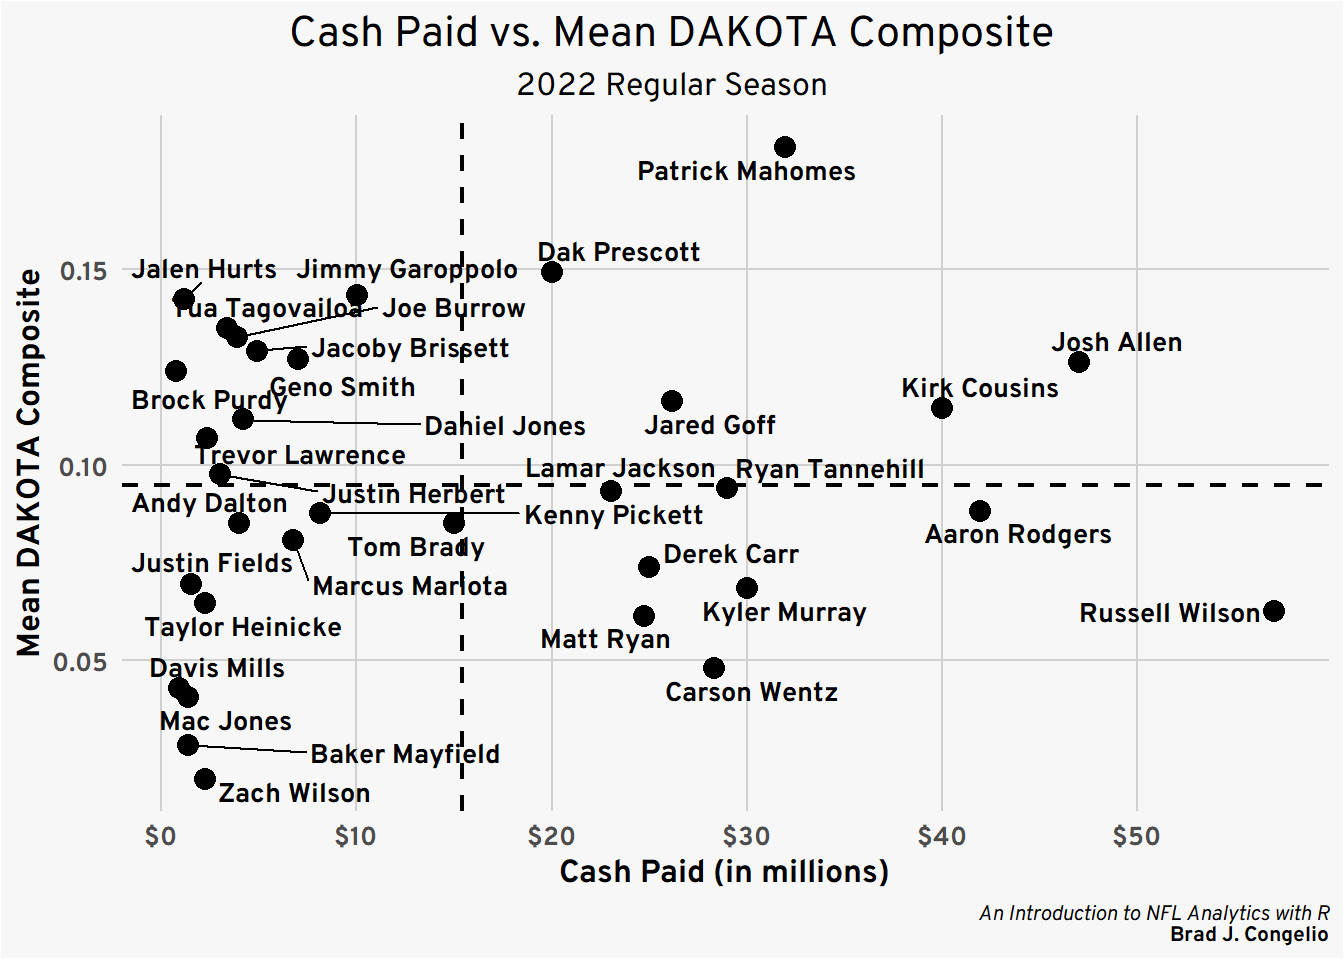
\includegraphics{03-nfl-analytics-functions_files/figure-pdf/cash-paid-dakota-plot-1.pdf}

}

\end{figure}

Those players in the upper-right quadrant (Mahomes, Allen, Cousins,
etc.) are among the highest paid quarterbacks in the league, but also
are the highest performing players based on the DAKOTA composite. On the
other hand, those QBs in the lower-right quadrant are - based on the
DAKOTA composite - overpaid relevant to their performance on the field.
The lower-left QBs are not highly paid, but also do not perform well.
Those players in the upper-left performed extremely well (some better
than those in the upper-right) but come with a team-friendly contract
(in terms of pure cash paid).

\hypertarget{exercises-1}{%
\section{Exercises}\label{exercises-1}}

\hypertarget{exercise-1-1}{%
\subsection{\texorpdfstring{\textbf{Exercise
1}}{Exercise 1}}\label{exercise-1-1}}

\begin{enumerate}
\def\labelenumi{\arabic{enumi}.}
\tightlist
\item
  Load data from the 2010 to 2022 regular seasons into a data frame
  titled \texttt{pbp}.
\item
  In a data frame titled \texttt{rushing\_success}, determine how many
  rushing attempts each offensive team had on 1st down.
\item
  Determine how many of those attempts resulted in a positive EPA
  (\texttt{success}).
\item
  Calculate the percentage of the results into a column titled
  \texttt{success\_pct}.
\item
  Arrange the results in descending order by \texttt{success\_pct}.
\end{enumerate}

\hypertarget{exercise-2-1}{%
\subsection{Exercise 2}\label{exercise-2-1}}

Load data from the 2022 regular season into a data frame titled
\texttt{pbp\_2022}.

\begin{enumerate}
\def\labelenumi{\arabic{enumi}.}
\tightlist
\item
  In a data frame titled \texttt{qb\_short\_third}, determine how many
  3rd down passing attempts each QB had.
\item
  Determine the number of times the QB's air yards was less than the
  required yards to go.
\item
  In a column titled \texttt{ay\_percent}, calculate the percentage of
  these results.
\item
  Filter the results to those QBs with 100 or more attempts.
\item
  Arrange the results in descending order by \texttt{ay\_percent}.
\end{enumerate}

\hypertarget{exercise-3-1}{%
\subsection{Exercise 3}\label{exercise-3-1}}

Tom Brady had a long and storied career, serving as a full-time started
in the NFL from 2001 to 2022. The \texttt{qb\_epa} metric gives a
quarterback credit for EPA up to the point where a receivers lost a
fumble after a completed catch. For this question, create data frame
titled \texttt{tom\_brady} and find Brady's average \texttt{qb\_epa} per
season, from 2001 to 2022. After, arrange in descending order by his
average QB EPA.

\hypertarget{exercise-4-1}{%
\subsection{Exercise 4}\label{exercise-4-1}}

Create a data frame titled \texttt{made\_field\_goals} and find, between
the 2000 and 2022 season, the number of field goal attempts and
percentage made on all kicks greater than 40-yards in distance.

\hypertarget{exercise-5-1}{%
\subsection{Exercise 5}\label{exercise-5-1}}

On December 11 of the 2005 season, Pittsburgh's Jerome Bettis trucked
Bears linebacker Brian Urlacher. You can view the play here:
\href{https://www.youtube.com/watch?v=u0mtG-8DWYk}{Bettis Trucks
Urlacher}. Using the \texttt{load\_pbp} function, find this specific
play (using the video for contextual clues). After, determine how much
win probability this individual play added (that is: the differnece
between \texttt{home\_wp} and \texttt{home\_wp\_post}.

\bookmarksetup{startatroot}

\hypertarget{data-visualization-with-nfl-data}{%
\chapter{Data Visualization with NFL
Data}\label{data-visualization-with-nfl-data}}

Effective data visualization is an important part of any data analysis
project as it helps in highlighting key insights into the data,
identifying trends, patterns, and anomalies, as while as allowing you to
communicate results to the outside world.

Jim Stikeleather, writing for the \emph{Harvard Business Review},
outlined three key elements that make a successful data visualization
(albeit, leaving \emph{us} to decide the definition of what a
``successful'' data visualization is). Despite that philosophical gap,
the three elements provided by Stikeleather are succinct enough to allow
us to build a framework in this chapter for how to successfully craft an
NFL analytics data visualization. In his piece, Stikeleather outlines
the following three characteristics of a successful data visualization:
it understands the audience, it sets up a clear framework, and it tells
a story (Stikeleather 2013).

To illustrate the importance of these three elements, let's take a look
at example visualizations using NFL data to further contextualize each
one.

\hypertarget{data-viz-must-understand-the-audience}{%
\section{Data Viz Must Understand the
Audience}\label{data-viz-must-understand-the-audience}}

As explained by Stikeleather, the core purpose of a data visualization
is to take ``great quantities of information'' and then convey that
information in such a way that it is ``easily assimilated by the
consumers of the information.'' In other words, the process of data
visualization should allow for a great quantity of data to be distilled
into an easily consumable (and understandable!) format.

Speaking specifically to NFL analytics, when doing visualizations we
must be conscious about whether or not the intended audience will
understand the terminology and concepts we use in the plot. For example,
most all NFL fans understand the ``non-advanced'' statistics in the
sport. But, when plots start using metrics such as EPA or completion
percentage over expected, for example, the audience looking at the plot
may very well have little understanding of what is being conveyed.

Because of this, any data viz I create never fails to include
``directables'' within the plot. These ``directables'' may be arrows
that indicate which trend on the plot are ``good'' or they can be text
within a scatterplot that explains what each quadrant means. Or, for
example, I sometimes include a textual explanation of the ``equation''
used to develop a metric as seen below:

\begin{figure}

{\centering 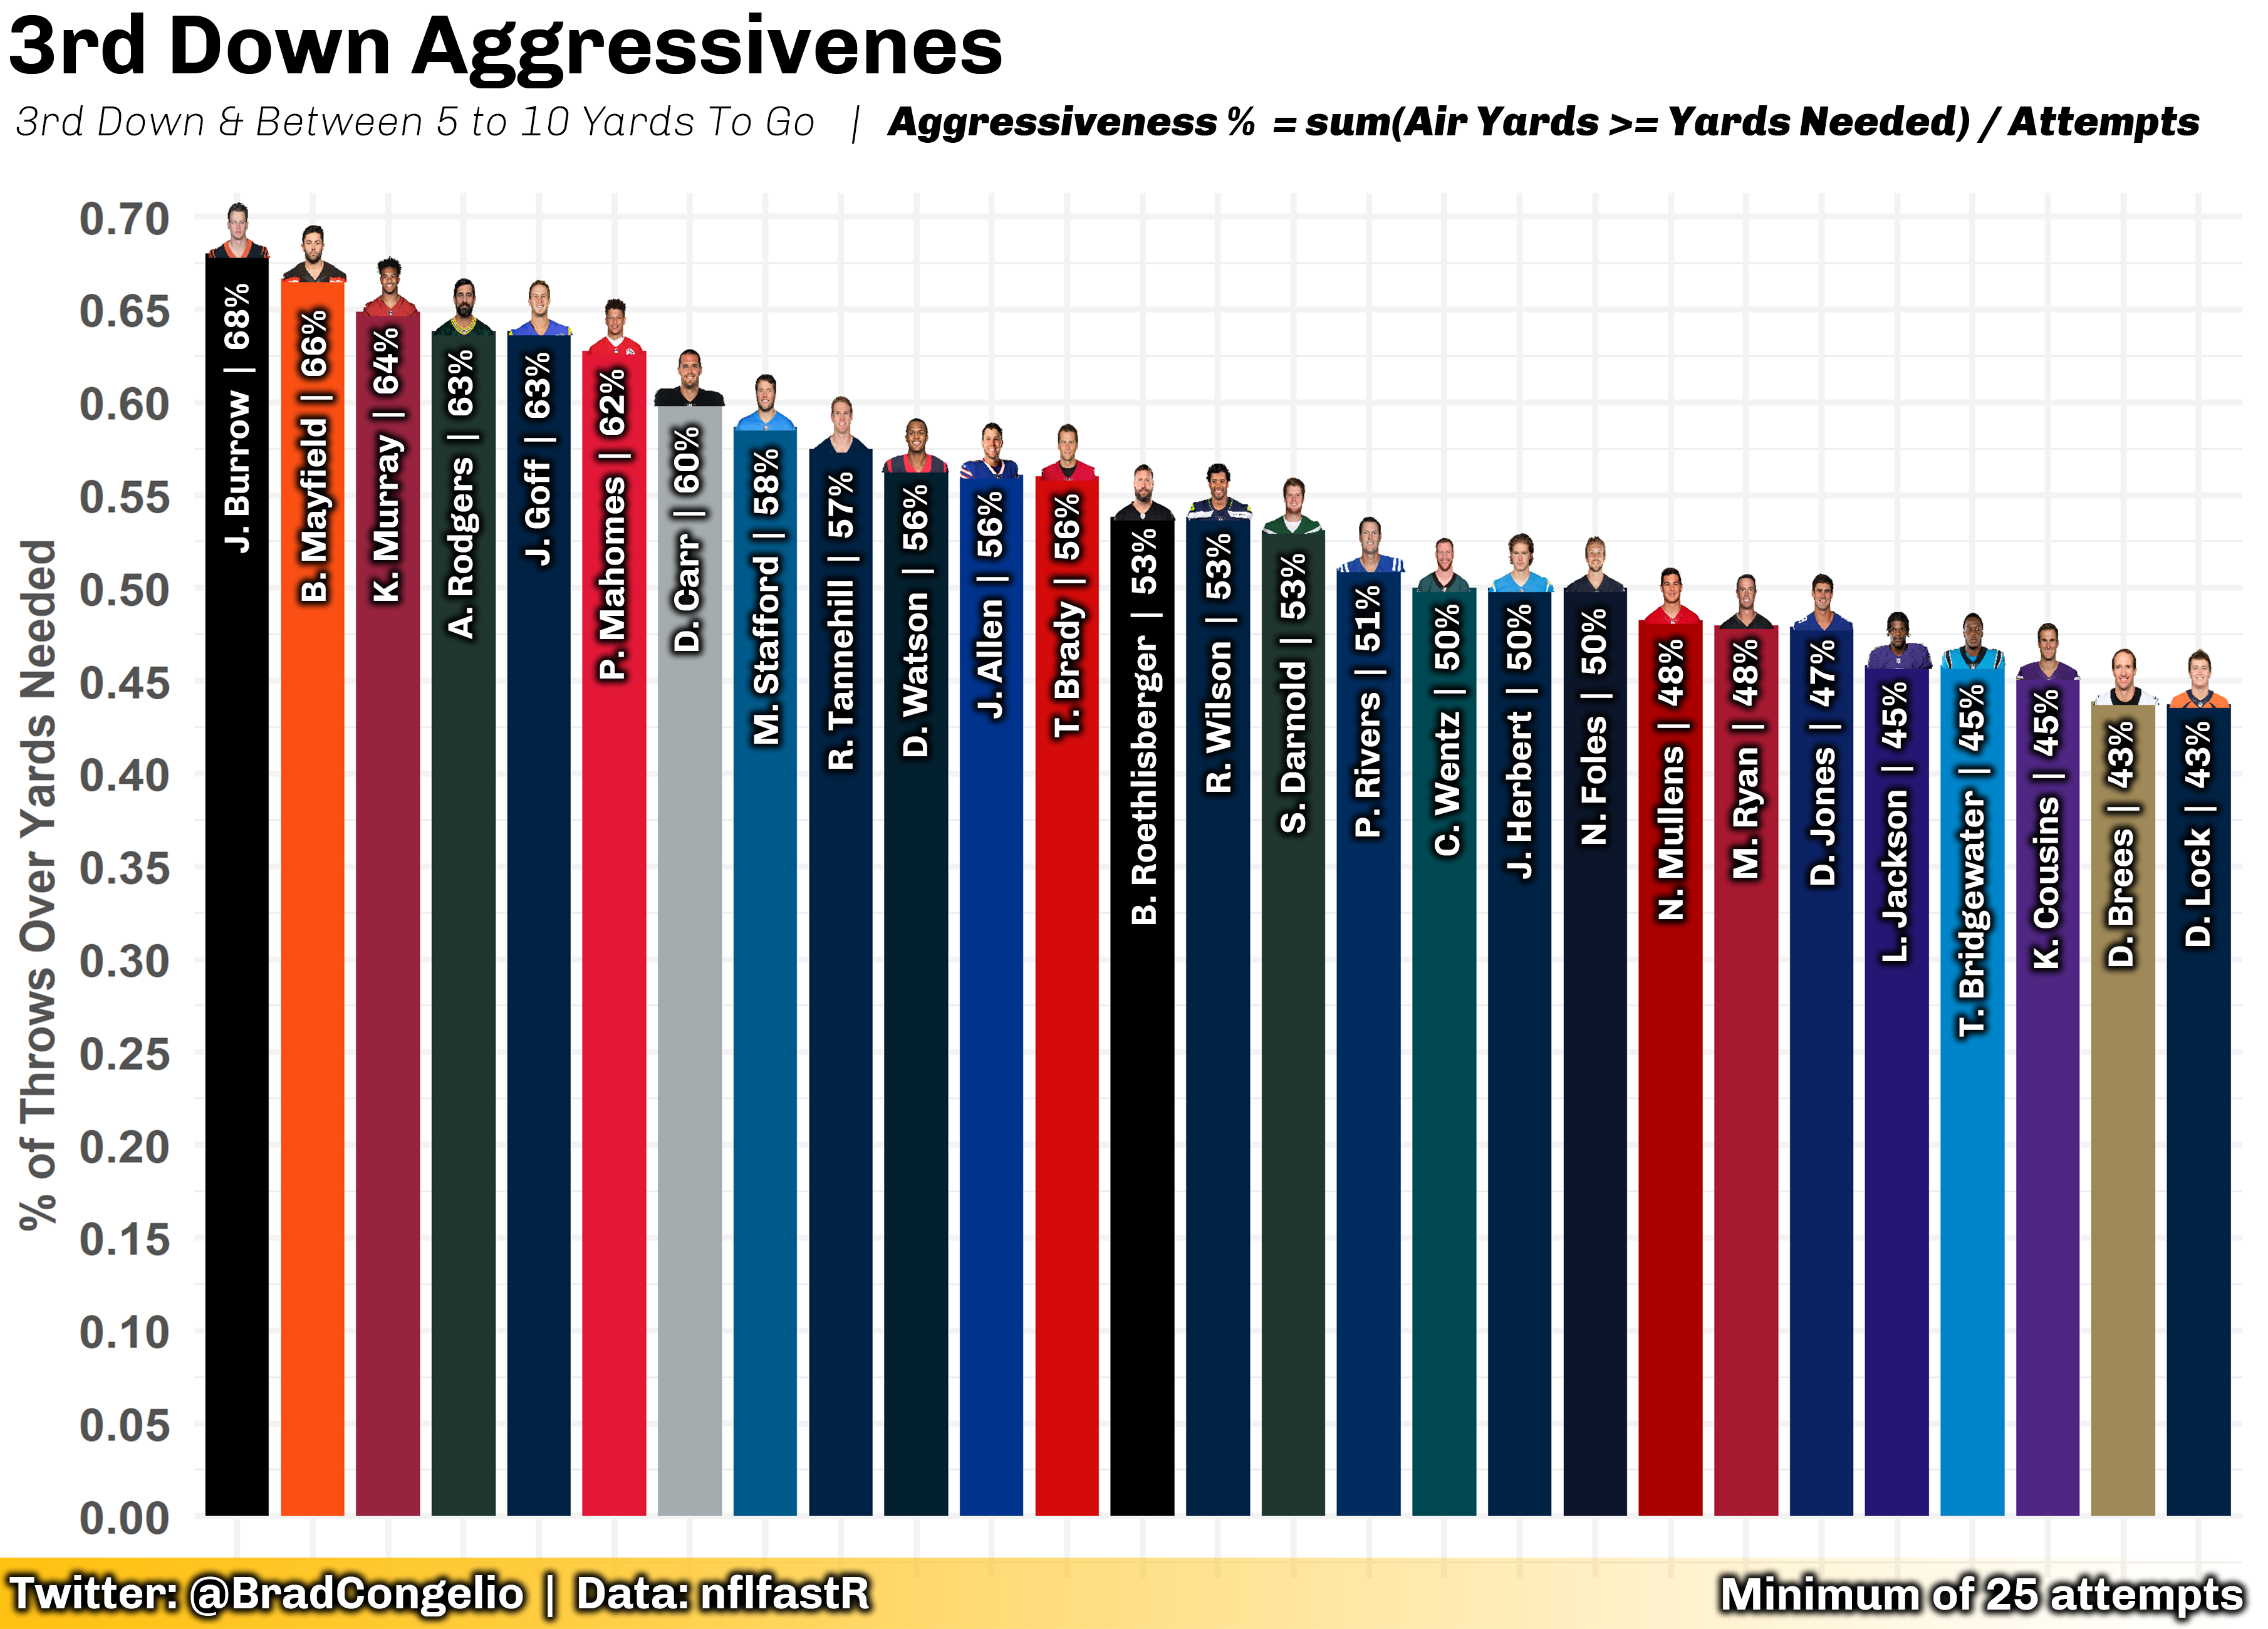
\includegraphics[width=4.58333in,height=\textheight]{images/finished-aggressiveness.png}

}

\end{figure}

The above plot explores which QBs, from the 2020 season, were most
aggressive on 3rd down with between 5 to 10 yards to go. Since
``aggressiveness'' is not a typical, day-to-day metric discussed by NFL
fans, I included a ``directable'' within the subtitle of the plot that
explained that the plot, first, was examining just 3rd down pass
attempts within a specific yard range. And, second, I made the decision
to include how ``aggressiveness'' was calculated by including the simple
equation within the subtitle as well. Doing so allows even the most
casual of NFL fans to easily understand what the plot is showing - in
this case, that Joe Burrow's 3rd down pass attempts with between 5 to 10
yards to go made it to the line of gain, or more, on 68\% of his
attempts. On the other hand, Drew Lock and Drew Brees were the least
aggressive QBs in the line based on the same metric.

\hypertarget{setting-up-for-data-viz}{%
\section{Setting Up for Data Viz}\label{setting-up-for-data-viz}}

While most of your journey through NFL analytics in this book required
you to use the \texttt{tidyverse} and a handful of other packages, the
process of creating compelling and meaningful data visualizations will
require you to utilize multitudes of other packages. Of course, the most
important is \texttt{ggplot2} which is already installed via the
\texttt{tidyverse}. However, in order to recreate the visualizations
included in this chapter, it is required that you install other R
packages. To install the necessary packages, you can run the following
code in RStudio:

\begin{Shaded}
\begin{Highlighting}[]
\FunctionTok{install.packages}\NormalTok{(}\FunctionTok{c}\NormalTok{(}\StringTok{"extrafont"}\NormalTok{,}
                   \StringTok{"ggrepel"}\NormalTok{,}
                   \StringTok{"ggimage"}\NormalTok{,}
                   \StringTok{"ggridges"}\NormalTok{,}
                   \StringTok{"ggtext"}\NormalTok{,}
                   \StringTok{"ggfx"}\NormalTok{,}
                   \StringTok{"geomtextpath"}\NormalTok{,}
                   \StringTok{"cropcircles"}\NormalTok{,}
                   \StringTok{"magick"}\NormalTok{,}
                   \StringTok{"glue"}\NormalTok{,}
                   \StringTok{"gt"}\NormalTok{,}
                   \StringTok{"gtExtras"}\NormalTok{))}
\end{Highlighting}
\end{Shaded}

\hypertarget{the-basics-of-using-ggplot2}{%
\section{\texorpdfstring{The Basics of Using
\texttt{ggplot2}}{The Basics of Using ggplot2}}\label{the-basics-of-using-ggplot2}}

The basics of any \texttt{ggplot} visualization involves three basic
calls to information in a data set as well as stipulation which type of
geom you would like to use:

\begin{enumerate}
\def\labelenumi{\arabic{enumi}.}
\tightlist
\item
  the data set to be used in the visualization
\item
  an aesthetic calls for the x-axis
\item
  an aesthetic call for the y-axis
\item
  your desired geom type
\end{enumerate}

\begin{Shaded}
\begin{Highlighting}[]
\FunctionTok{ggplot}\NormalTok{(}\AttributeTok{data =} \StringTok{\textquotesingle{}dataset\_name\textquotesingle{}}\NormalTok{, }\FunctionTok{aes}\NormalTok{(}\AttributeTok{x =} \StringTok{\textquotesingle{}x\_axsis\textquotesingle{}}\NormalTok{, }\AttributeTok{y =} \StringTok{\textquotesingle{}y\_axis\textquotesingle{}}\NormalTok{)) }\SpecialCharTok{+}
  \FunctionTok{geom\_type}\NormalTok{()}
\end{Highlighting}
\end{Shaded}

To showcase this, let's use data from Sports Info Solutions that
pertains quarterback statistic when using play action versus when not
using play action. To start, collect the data using the \texttt{vroom}
function.

\begin{Shaded}
\begin{Highlighting}[]
\NormalTok{play\_action\_data }\OtherTok{\textless{}{-}}
  \FunctionTok{vroom}\NormalTok{(}\StringTok{"https://raw.githubusercontent.com/bcongelio/nfl{-}analytics{-}with{-}r{-}book/origin/example\_data/csv/play\_action\_data.csv"}\NormalTok{)}
\end{Highlighting}
\end{Shaded}

To provide an easy-to-understand example of building a visualization
with \texttt{ggplot}, let's use each QB's total yardage when using play
action and when not. In this case, our two variable names are
\texttt{yds} and \texttt{pa\_yds} with the \texttt{yds} variable being
place on the x-axis and the \texttt{pa\_yds} variable being placed on
the y-axis.

\begin{tcolorbox}[enhanced jigsaw, left=2mm, toprule=.15mm, opacitybacktitle=0.6, leftrule=.75mm, bottomrule=.15mm, colbacktitle=quarto-callout-tip-color!10!white, breakable, colback=white, bottomtitle=1mm, toptitle=1mm, title=\textcolor{quarto-callout-tip-color}{\faLightbulb}\hspace{0.5em}{Tip}, coltitle=black, titlerule=0mm, arc=.35mm, opacityback=0, colframe=quarto-callout-tip-color-frame, rightrule=.15mm]

It is important to remember which axis is which as you begin to learn
using \texttt{ggplot}:

The x-axis is the horizontal axis that runs left-to-right.

The y-axis is the vertical axis that runs top-to-bottom.

\end{tcolorbox}

\begin{Shaded}
\begin{Highlighting}[]
\FunctionTok{ggplot}\NormalTok{(}\AttributeTok{data =}\NormalTok{ play\_action\_data, }\FunctionTok{aes}\NormalTok{(}\AttributeTok{x =}\NormalTok{ yds, }\AttributeTok{y =}\NormalTok{ pa\_yds)) }\SpecialCharTok{+}
  \FunctionTok{geom\_point}\NormalTok{()}
\end{Highlighting}
\end{Shaded}

\begin{figure}[H]

{\centering 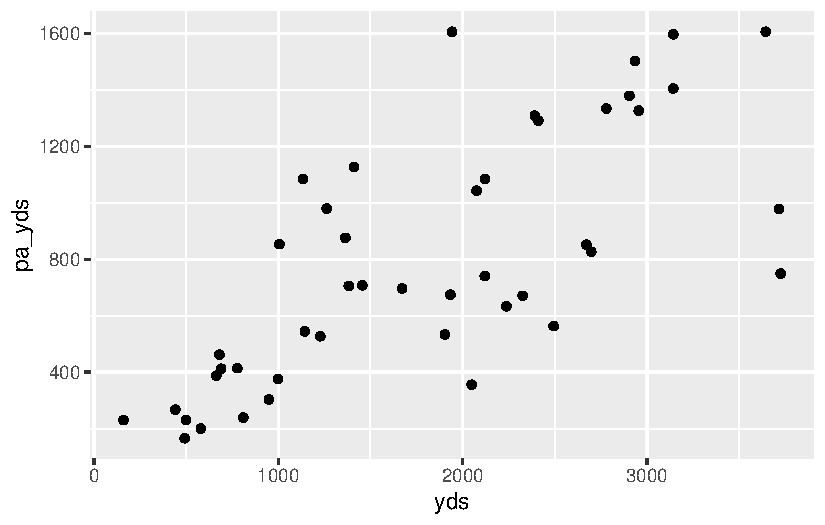
\includegraphics{04-nfl-analytics-visualization_files/figure-pdf/example-pa-action-plot-1.pdf}

}

\end{figure}

\hypertarget{building-a-data-viz-a-step-by-step-process}{%
\section{Building A Data Viz: A Step-by-Step
Process}\label{building-a-data-viz-a-step-by-step-process}}

The outputted scatter plot is an excellent starting point for a more
finely detailed visualization. While we are able to see the relationship
between non-play action passing yards and those attempts that included
play action, we are unable to discern which specific point is which
quarterback - among other issues. To provide more detail and to
``prettify'' the plot, let's discuss doing the following:

\begin{tcolorbox}[enhanced jigsaw, left=2mm, toprule=.15mm, opacitybacktitle=0.6, leftrule=.75mm, bottomrule=.15mm, colbacktitle=quarto-callout-note-color!10!white, breakable, colback=white, bottomtitle=1mm, toptitle=1mm, title=\textcolor{quarto-callout-note-color}{\faInfo}\hspace{0.5em}{Note}, coltitle=black, titlerule=0mm, arc=.35mm, opacityback=0, colframe=quarto-callout-note-color-frame, rightrule=.15mm]

Our data visualization ``to do list'':

\begin{enumerate}
\def\labelenumi{\arabic{enumi}.}
\tightlist
\item
  Adding team colors to each point.
\item
  Increasing the size of each point.
\item
  Adding player names to each point.
\item
  Increasing the number of ticks on each axis.
\item
  Provide the numeric values in correct format (that is, including a
  \texttt{,} to correctly show thousands).
\item
  Rename the title of each axis.
\item
  Provide a title, subtitle, and caption for the plot.
\item
  Add mean lines to both the x-axis and y-axis
\item
  Change \texttt{theme} elements to make data viz more appealing.
\end{enumerate}

\end{tcolorbox}

\hypertarget{adding-team-colors-to-each-point}{%
\subsection{Adding Team Colors to Each
Point}\label{adding-team-colors-to-each-point}}

\begin{tcolorbox}[enhanced jigsaw, left=2mm, toprule=.15mm, opacitybacktitle=0.6, leftrule=.75mm, bottomrule=.15mm, colbacktitle=quarto-callout-note-color!10!white, breakable, colback=white, bottomtitle=1mm, toptitle=1mm, title=\textcolor{quarto-callout-note-color}{\faInfo}\hspace{0.5em}{Note}, coltitle=black, titlerule=0mm, arc=.35mm, opacityback=0, colframe=quarto-callout-note-color-frame, rightrule=.15mm]

Much like anything in the R language, there are multiple ways to go
about add team colors (and logos, player headshots, etc.) to
visualizations.

First, we can merge team color information into our
\texttt{play\_action\_data} and then manually set the colors in our
\texttt{geom\_point} call.

Second, we can conduct the same merge but then use the
\texttt{nflplotRr} package (which is part of the \texttt{nflverse}) to
bring the colors in.

Both examples will be included in the below example.

\end{tcolorbox}

To start, we will load team information using the \texttt{load\_teams}
function within \texttt{nflreadr}. In this case, we are requesting that
the package provide only the 32 current NFL teams with by including the
\texttt{current\ =\ TRUE} argument. Conversely, setting the argument to
\texttt{current\ =\ FALSE} will result in historical NFL teams being
included in the data (the Oakland Raiders and St.~Louis Rams, for
example, will be included in the data). We will also use the
\texttt{select()} verb from \texttt{dplyr} to gather just the variables
we know we will need (\texttt{team\_abbr}, \texttt{team\_nick},
\texttt{team\_color}, and \texttt{team\_color2}.

\begin{tcolorbox}[enhanced jigsaw, left=2mm, toprule=.15mm, opacitybacktitle=0.6, leftrule=.75mm, bottomrule=.15mm, colbacktitle=quarto-callout-important-color!10!white, breakable, colback=white, bottomtitle=1mm, toptitle=1mm, title=\textcolor{quarto-callout-important-color}{\faExclamation}\hspace{0.5em}{Important}, coltitle=black, titlerule=0mm, arc=.35mm, opacityback=0, colframe=quarto-callout-important-color-frame, rightrule=.15mm]

We are only including the \texttt{team\_abbr} variable in this example
because we are going to create the plot both with and without the use of
\texttt{nflplotR}. As of the writing of this book, the newest
development version of the package is 1.1.0.9004 and does not yet (if
ever) provide support to use team nicknames. Because of this, we must
include \texttt{team\_abbr} in our merge since it is the team name
version that is standardized for use in \texttt{nflplotr}.

\end{tcolorbox}

After collecting the team information needed, we can conduct a
\texttt{left\_join()} to match the information by \texttt{team} in
\texttt{play\_action\_data} and \texttt{team\_nick} in the team
information from \texttt{load\_teams()} and then confirm the merge was
successful by viewing the columns names in \texttt{play\_action\_data}
with \texttt{colnames()}.

\begin{Shaded}
\begin{Highlighting}[]
\NormalTok{teams }\OtherTok{\textless{}{-}}\NormalTok{ nflreadr}\SpecialCharTok{::}\FunctionTok{load\_teams}\NormalTok{(}\AttributeTok{current =} \ConstantTok{TRUE}\NormalTok{) }\SpecialCharTok{\%\textgreater{}\%}
  \FunctionTok{select}\NormalTok{(team\_abbr, team\_nick, team\_color, team\_color2)}

\NormalTok{play\_action\_data }\OtherTok{\textless{}{-}}\NormalTok{ play\_action\_data }\SpecialCharTok{\%\textgreater{}\%}
  \FunctionTok{left\_join}\NormalTok{(teams, }\AttributeTok{by =} \FunctionTok{c}\NormalTok{(}\StringTok{"team"} \OtherTok{=} \StringTok{"team\_nick"}\NormalTok{))}

\FunctionTok{colnames}\NormalTok{(play\_action\_data)}
\end{Highlighting}
\end{Shaded}

With the team color information now built into our
\texttt{play\_action\_data}, we can incorporate the team color specific
to each point by including the \texttt{color} argument within our
\texttt{geom\_point}.

\begin{Shaded}
\begin{Highlighting}[]
\FunctionTok{ggplot}\NormalTok{(}\AttributeTok{data =}\NormalTok{ play\_action\_data, }\FunctionTok{aes}\NormalTok{(}\AttributeTok{x =}\NormalTok{ yds, }\AttributeTok{y =}\NormalTok{ pa\_yds)) }\SpecialCharTok{+}
  \FunctionTok{geom\_point}\NormalTok{(}\AttributeTok{color =}\NormalTok{ play\_action\_data}\SpecialCharTok{$}\NormalTok{team\_color)}
\end{Highlighting}
\end{Shaded}

\begin{figure}[H]

{\centering 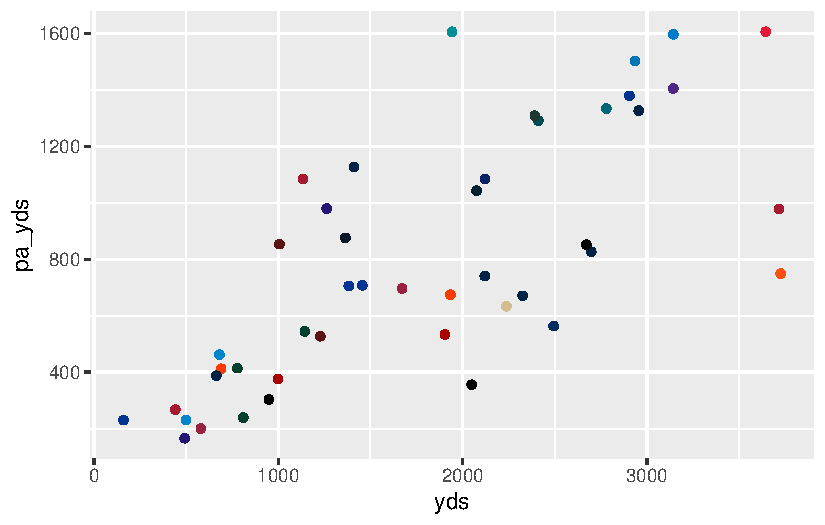
\includegraphics{04-nfl-analytics-visualization_files/figure-pdf/adding-team-color-no-nflplotr-1.pdf}

}

\end{figure}

\begin{tcolorbox}[enhanced jigsaw, left=2mm, toprule=.15mm, opacitybacktitle=0.6, leftrule=.75mm, bottomrule=.15mm, colbacktitle=quarto-callout-important-color!10!white, breakable, colback=white, bottomtitle=1mm, toptitle=1mm, title=\textcolor{quarto-callout-important-color}{\faExclamation}\hspace{0.5em}{Important}, coltitle=black, titlerule=0mm, arc=.35mm, opacityback=0, colframe=quarto-callout-important-color-frame, rightrule=.15mm]

You may notice that we used the the \texttt{\$} special operator to
extract the \texttt{team\_color} information within our
\texttt{play\_action\_data} data frame. This is an extremely important
distinction, as using the \texttt{aes()} argument from \texttt{ggplot}
and not using the \texttt{\$} operator will result in a custom scale
color being applied to each team, without the correct team colors
associating with the correct team.

To see this for yourself, you can run the example following code.
Remember, this is an incorrect approach and serves to only highlight why
the \texttt{\$} special operator was used in the above code.

\begin{Shaded}
\begin{Highlighting}[]
\FunctionTok{ggplot}\NormalTok{(}\AttributeTok{data =}\NormalTok{ play\_action\_data, }\FunctionTok{aes}\NormalTok{(}\AttributeTok{x =}\NormalTok{ yds, }\AttributeTok{y =}\NormalTok{ pa\_yds)) }\SpecialCharTok{+}
  \FunctionTok{geom\_point}\NormalTok{(}\FunctionTok{aes}\NormalTok{(}\AttributeTok{color =}\NormalTok{ team\_color))}
\end{Highlighting}
\end{Shaded}

\begin{figure}[H]

{\centering 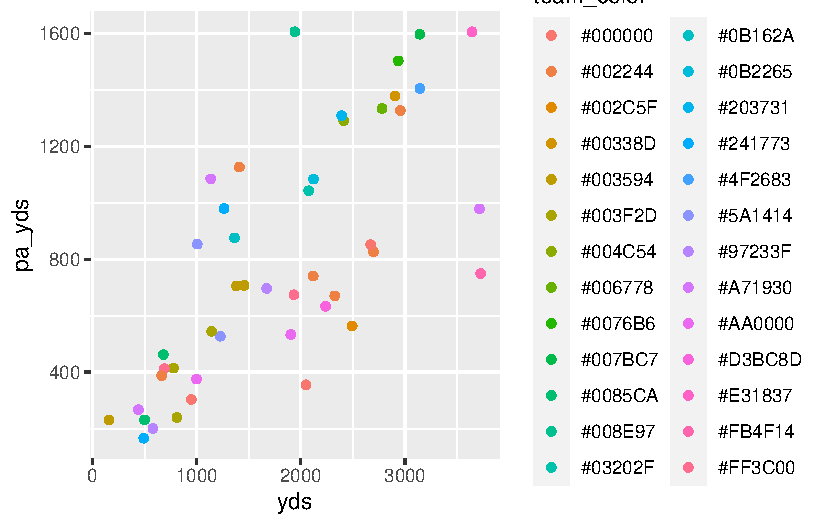
\includegraphics{04-nfl-analytics-visualization_files/figure-pdf/incorrect-use-of-aes-1.pdf}

}

\end{figure}

\end{tcolorbox}

As mentioned, the same result can be achieved using the
\texttt{nflplotR} package. The following code will do so:

\begin{Shaded}
\begin{Highlighting}[]
\FunctionTok{ggplot}\NormalTok{(}\AttributeTok{data =}\NormalTok{ play\_action\_data, }\FunctionTok{aes}\NormalTok{(}\AttributeTok{x =}\NormalTok{ yds, }\AttributeTok{y =}\NormalTok{ pa\_yds)) }\SpecialCharTok{+}
  \FunctionTok{geom\_point}\NormalTok{(}\FunctionTok{aes}\NormalTok{(}\AttributeTok{color =}\NormalTok{ team\_abbr)) }\SpecialCharTok{+}
\NormalTok{  nflplotR}\SpecialCharTok{::}\FunctionTok{scale\_color\_nfl}\NormalTok{(}\AttributeTok{type =} \StringTok{"primary"}\NormalTok{)}
\end{Highlighting}
\end{Shaded}

\begin{figure}[H]

{\centering 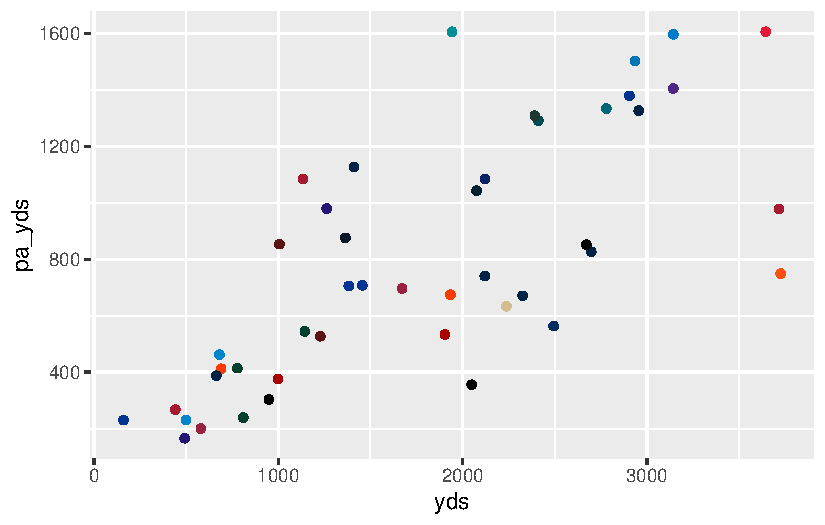
\includegraphics{04-nfl-analytics-visualization_files/figure-pdf/adding-color-with-nflplotr-1.pdf}

}

\end{figure}

In the above example, you will notice that we are including the team
color information in an \texttt{aes()} call within the
\texttt{geom\_point()} function. This is because we ultimately control
the specific of the custom scale through the use of
\texttt{scale\_color\_nfl} in the \texttt{nflplotR} package, which also
allows us to select whether we want to display the primary or secondary
team color.

Given the two examples above, a couple items regarding the use of
\texttt{nflplotR} should become apparent.

\begin{enumerate}
\def\labelenumi{\arabic{enumi}.}
\tightlist
\item
  If your data already includes team names in \texttt{team\_abbr} format
  (that is: BAL, CIN, DET, DAL, etc.), then using \texttt{nflplotR} is
  likely a more efficient option as you do not need to merge in team
  color information. In other words, our \texttt{play\_action\_data}
  information could contain just the variables for \texttt{player},
  \texttt{team\_abbr}, \texttt{yds}, and \texttt{pa\_yds} and
  \texttt{nflplotR} would still work as the package, ``behind the
  scenes'', will automatically correlate the \texttt{team\_abbr} with
  the correct color for each team.
\item
  However, if your data does not include teams in \texttt{team\_abbr}
  format and you must merge in information manually, it is likely more
  efficient to use the \texttt{\$} special operator to bring the team
  colors in without using the \texttt{aes()} call within
  \texttt{geom\_point()}.
\end{enumerate}

Finally, because we have both \texttt{team\_color} and
\texttt{team\_color2} - the primary and secondary colors for each team -
in the data, we can get fancy and create points that are filled with the
primary team color and outlined by the secondary team color. Doing so
simply requires changing the type of our \texttt{geom\_point}. In the
below example, we are specifying that we want a specific type of
\texttt{geom\_point} by using \texttt{shape\ =\ 21} and then providing
the \texttt{fill} color and the outline color with \texttt{color}. In
each case, we are again using the \texttt{\$} special operator to select
the primary and secondary color associated with each team.

\begin{Shaded}
\begin{Highlighting}[]
\FunctionTok{ggplot}\NormalTok{(}\AttributeTok{data =}\NormalTok{ play\_action\_data, }\FunctionTok{aes}\NormalTok{(}\AttributeTok{x =}\NormalTok{ yds, }\AttributeTok{y =}\NormalTok{ pa\_yds)) }\SpecialCharTok{+}
  \FunctionTok{geom\_point}\NormalTok{(}\AttributeTok{shape =} \DecValTok{21}\NormalTok{,}
             \AttributeTok{fill =}\NormalTok{ play\_action\_data}\SpecialCharTok{$}\NormalTok{team\_color,}
             \AttributeTok{color =}\NormalTok{ play\_action\_data}\SpecialCharTok{$}\NormalTok{team\_color2)}
\end{Highlighting}
\end{Shaded}

\begin{figure}[H]

{\centering 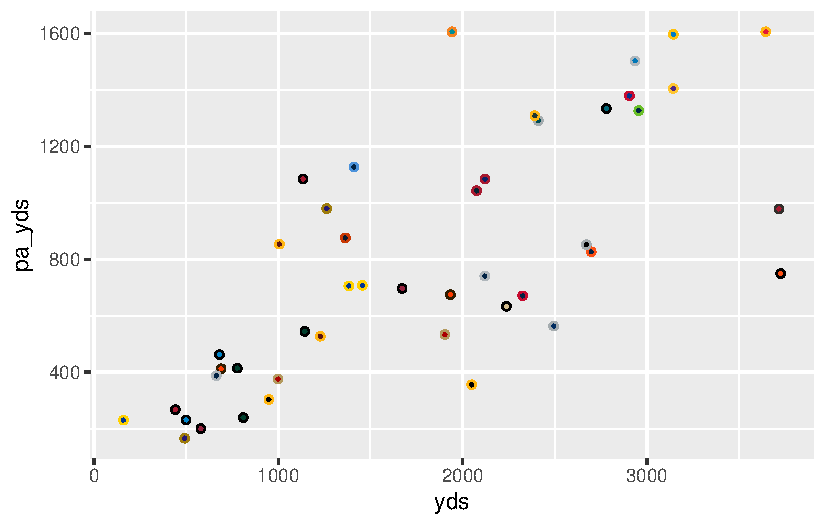
\includegraphics{04-nfl-analytics-visualization_files/figure-pdf/adding-shape-21-to-plot-1.pdf}

}

\end{figure}

With team colors correctly associated with each point, we can turn back
to our ``to do list'' to see what part of the job is next.

\begin{tcolorbox}[enhanced jigsaw, left=2mm, toprule=.15mm, opacitybacktitle=0.6, leftrule=.75mm, bottomrule=.15mm, colbacktitle=quarto-callout-note-color!10!white, breakable, colback=white, bottomtitle=1mm, toptitle=1mm, title=\textcolor{quarto-callout-note-color}{\faInfo}\hspace{0.5em}{Note}, coltitle=black, titlerule=0mm, arc=.35mm, opacityback=0, colframe=quarto-callout-note-color-frame, rightrule=.15mm]

Our data visualization ``to do list'':

\begin{enumerate}
\def\labelenumi{\arabic{enumi}.}
\item
  \st{Adding team colors to each point.}
\item
  Increasing the size of each point.
\item
  Adding player names to each point.
\item
  Increasing the number of ticks on each axis.
\item
  Provide the numeric values in correct format (that is, including a ,
  to correctly show thousands).
\item
  Rename the title of each axis.
\item
  Provide a title, subtitle, and caption for the plot.
\item
  Add mean lines to both the x-axis and y-axis.
\item
  Change \texttt{theme} elements to make data viz more appealing.
\end{enumerate}

\end{tcolorbox}

\hypertarget{increasing-the-size-of-each-point}{%
\subsection{Increasing The Size of Each
Point}\label{increasing-the-size-of-each-point}}

Determining when and how to resize the individual points in a
scatterplot is a multifaceted decision. To that end, there is no hard
and fast rule for doing so as it depends on both the specific goals and
context of the visualization. There are, however, some general
guidelines to keep in mind:

\begin{enumerate}
\def\labelenumi{\arabic{enumi}.}
\tightlist
\item
  Data density: if you have a lot of data points within your plot,
  making the points smaller may help to reduce issues of
  overlapping/overplotting. Not only is this more aesthetically
  pleasing, but it can also help in making it easier to see patterns.
\item
  Importance of individual points: if certain points within the
  scatterplot are important, we may want to increase the size of those
  specific points to make them standout.
\item
  Visual aesthetics: the size of the points can be adjusted simply for
  visual appeal.
\item
  Contextual factors: can the size of the points be used to highlight
  even more uniqueness in the data? For example, given the right data
  structure, we can size individual dots to show the spread in total
  attempts across the quarterbacks.
\end{enumerate}

Given the above guidelines, the resizing of the points in our
\texttt{play\_action\_data} data frame is going to be a strictly
aesthetic decision. We cannot, as mentioned above, alter the size of
each specific points based on each quarterback's number of attempts as
the data provides attempts for \emph{both} play action and non-play
action passes. Moreover, we \emph{could}~create a new column that add
both attempt numbers to get a QB's cumulative total but that does not
have a distinct correlation to the data on either axis.

\begin{tcolorbox}[enhanced jigsaw, left=2mm, toprule=.15mm, opacitybacktitle=0.6, leftrule=.75mm, bottomrule=.15mm, colbacktitle=quarto-callout-caution-color!10!white, breakable, colback=white, bottomtitle=1mm, toptitle=1mm, title=\textcolor{quarto-callout-caution-color}{\faFire}\hspace{0.5em}{Caution}, coltitle=black, titlerule=0mm, arc=.35mm, opacityback=0, colframe=quarto-callout-caution-color-frame, rightrule=.15mm]

For the sake of educational purposes, we can alter the size of each
specific point to correlate to the total number of play action attempts
for each quarterback (and then divide this by 25 in order to decrease
the size of the points to fit them all onto the plot).

Again: it is important to point out that this not a good approach to
data visualization, as the size of the dots correlates to just one of
the variables being explored in the plot.

\begin{Shaded}
\begin{Highlighting}[]
\FunctionTok{ggplot}\NormalTok{(}\AttributeTok{data =}\NormalTok{ play\_action\_data, }\FunctionTok{aes}\NormalTok{(}\AttributeTok{x =}\NormalTok{ yds, }\AttributeTok{y =}\NormalTok{ pa\_yds)) }\SpecialCharTok{+}
  \FunctionTok{geom\_point}\NormalTok{(}\AttributeTok{shape =} \DecValTok{21}\NormalTok{,}
             \AttributeTok{fill =}\NormalTok{ play\_action\_data}\SpecialCharTok{$}\NormalTok{team\_color,}
             \AttributeTok{color =}\NormalTok{ play\_action\_data}\SpecialCharTok{$}\NormalTok{team\_color2,}
             \AttributeTok{size =}\NormalTok{ play\_action\_data}\SpecialCharTok{$}\NormalTok{pa\_att }\SpecialCharTok{/} \DecValTok{25}\NormalTok{)}
\end{Highlighting}
\end{Shaded}

\begin{figure}[H]

{\centering 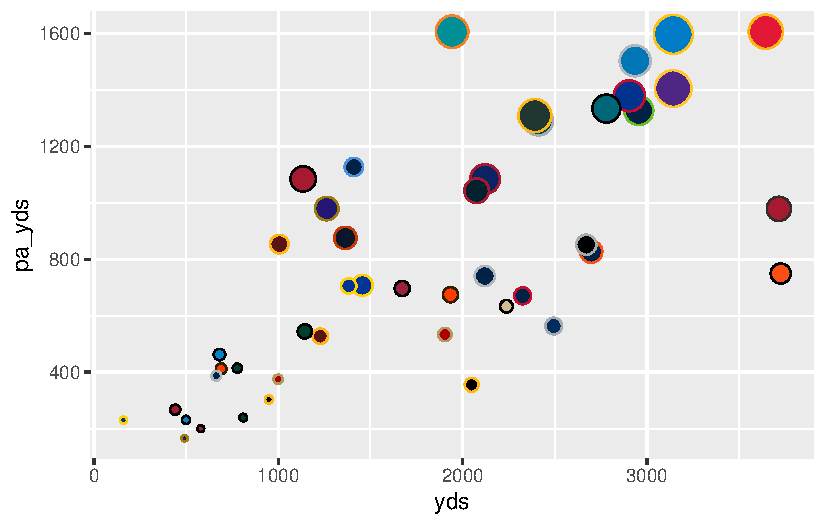
\includegraphics{04-nfl-analytics-visualization_files/figure-pdf/incorrect-use-of-sizing-1.pdf}

}

\end{figure}

\end{tcolorbox}

In order to maintain correct visualization standards, we can resize the
points for nothing more than aesthetic purposes (that is: making them
bigger so they are easier to see). To do so, we still add the
\texttt{size} argument to our \texttt{geom\_point} but simply provide a
numeric value to apply uniformly across all the points. To process of
selecting the numeric value is a case of trial and error - inputting and
running, changing and running, and changing and running again until you
find the size that provides easier to see points without adding overlap
into the visualization.

\begin{Shaded}
\begin{Highlighting}[]
\FunctionTok{ggplot}\NormalTok{(}\AttributeTok{data =}\NormalTok{ play\_action\_data, }\FunctionTok{aes}\NormalTok{(}\AttributeTok{x =}\NormalTok{ yds, }\AttributeTok{y =}\NormalTok{ pa\_yds)) }\SpecialCharTok{+}
  \FunctionTok{geom\_point}\NormalTok{(}\AttributeTok{shape =} \DecValTok{21}\NormalTok{,}
             \AttributeTok{fill =}\NormalTok{ play\_action\_data}\SpecialCharTok{$}\NormalTok{team\_color,}
             \AttributeTok{color =}\NormalTok{ play\_action\_data}\SpecialCharTok{$}\NormalTok{team\_color2,}
             \AttributeTok{size =} \FloatTok{4.5}\NormalTok{)}
\end{Highlighting}
\end{Shaded}

\begin{figure}[H]

{\centering 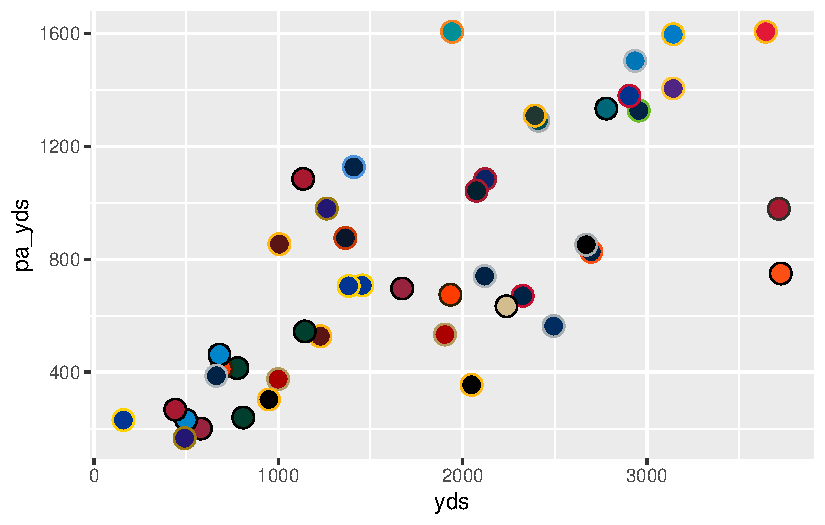
\includegraphics{04-nfl-analytics-visualization_files/figure-pdf/adding-correct-size-to-points-1.pdf}

}

\end{figure}

With the size of each point adequately adjusted, we can move on to the
next part of our data visualization ``to do list.''

\begin{tcolorbox}[enhanced jigsaw, left=2mm, toprule=.15mm, opacitybacktitle=0.6, leftrule=.75mm, bottomrule=.15mm, colbacktitle=quarto-callout-note-color!10!white, breakable, colback=white, bottomtitle=1mm, toptitle=1mm, title=\textcolor{quarto-callout-note-color}{\faInfo}\hspace{0.5em}{Note}, coltitle=black, titlerule=0mm, arc=.35mm, opacityback=0, colframe=quarto-callout-note-color-frame, rightrule=.15mm]

Our data visualization ``to do list'':

\begin{enumerate}
\def\labelenumi{\arabic{enumi}.}
\item
  \st{Adding team colors to each point.}
\item
  \st{Increasing the size of each point.}
\item
  Adding player names to each point.
\item
  Increasing the number of ticks on each axis.
\item
  Provide the numeric values in correct format (that is, including a ,
  to correctly show thousands).
\item
  Rename the title of each axis.
\item
  Provide a title, subtitle, and caption for the plot.
\item
  Add mean lines to both the x-axis and y-axis.
\item
  Change \texttt{theme} elements to make data viz more appealing.
\end{enumerate}

\end{tcolorbox}

\hypertarget{adding-player-names-to-each-point}{%
\subsection{Adding Player Names to Each
Point}\label{adding-player-names-to-each-point}}

While the our current plot includes team-specific colors for the points,
we are still not able to discern - for the most part - which player
belongs to which point. To rectify this, we will turn to using the
\texttt{ggrepel} package, which is designed to improve the readability
of text labels on plots by automatically repelling overlapping labels,
if any. \texttt{ggrepel} operates out of two main functions:
\texttt{geom\_text\_repel} and \texttt{geom\_label\_repel}. Both provide
the same end result, with the core different being
\texttt{geom\_label\_repel} adding a customized label under each
player's name.

We can do a bare minimum addition of the player names by adding one
additional line of code using \texttt{geom\_text\_repel}, wrapping it in
an \texttt{aes()} call, and specifying which variable in the
\texttt{play\_action\_data} is the \texttt{label} we would like to
display.

\begin{Shaded}
\begin{Highlighting}[]
\FunctionTok{ggplot}\NormalTok{(}\AttributeTok{data =}\NormalTok{ play\_action\_data, }\FunctionTok{aes}\NormalTok{(}\AttributeTok{x =}\NormalTok{ yds, }\AttributeTok{y =}\NormalTok{ pa\_yds)) }\SpecialCharTok{+}
  \FunctionTok{geom\_point}\NormalTok{(}\AttributeTok{shape =} \DecValTok{21}\NormalTok{,}
             \AttributeTok{fill =}\NormalTok{ play\_action\_data}\SpecialCharTok{$}\NormalTok{team\_color,}
             \AttributeTok{color =}\NormalTok{ play\_action\_data}\SpecialCharTok{$}\NormalTok{team\_color2,}
             \AttributeTok{size =} \FloatTok{4.5}\NormalTok{) }\SpecialCharTok{+}
  \FunctionTok{geom\_text\_repel}\NormalTok{(}\FunctionTok{aes}\NormalTok{(}\AttributeTok{label =}\NormalTok{ player))}
\end{Highlighting}
\end{Shaded}

\begin{verbatim}
Warning: ggrepel: 4 unlabeled data points (too many overlaps). Consider
increasing max.overlaps
\end{verbatim}

\begin{figure}[H]

{\centering 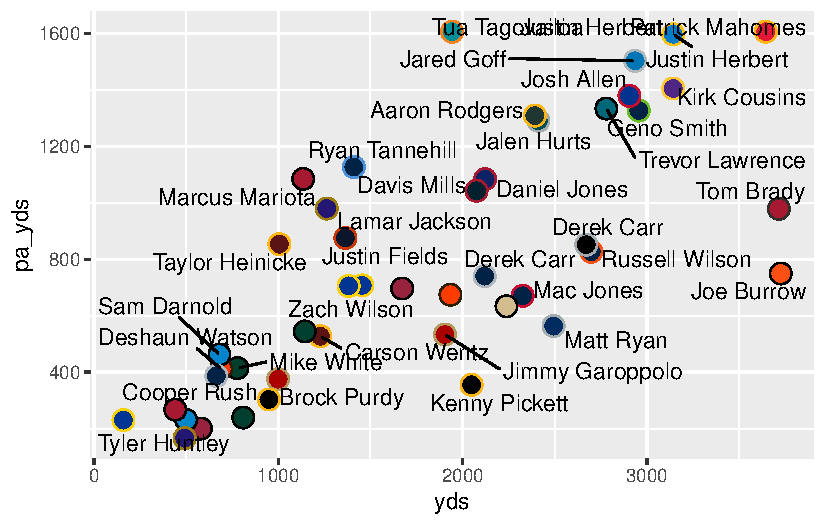
\includegraphics{04-nfl-analytics-visualization_files/figure-pdf/basic-addition-of-player-name-1.pdf}

}

\end{figure}

While it is a good first attempt at adding the names, many of them are
awkwardly close to the respective point. Luckily, the \texttt{ggrepel}
package provides plenty of built-in customization options:

\begin{longtable}[]{@{}
  >{\centering\arraybackslash}p{(\columnwidth - 2\tabcolsep) * \real{0.4077}}
  >{\centering\arraybackslash}p{(\columnwidth - 2\tabcolsep) * \real{0.5923}}@{}}
\toprule\noalign{}
\begin{minipage}[b]{\linewidth}\centering
\texttt{ggrepel} Option\footnote{As listed on the \texttt{ggrepel}
  website: \url{https://ggrepel.slowkow.com/articles/examples.html}}
\end{minipage} & \begin{minipage}[b]{\linewidth}\centering
Description of Option
\end{minipage} \\
\midrule\noalign{}
\endhead
\bottomrule\noalign{}
\endlastfoot
seed & a random numeric seed number for the purposes of recreating the
same layout \\
force & force of repulsion between overlapping text labels \\
force\_pull & force of attraction between each text label and its data
point \\
direction & move the text labels in either ``x'' or ``y'' directions \\
nudge\_x & adjust the starting x-axis starting position of the label \\
nudge\_y & adjust the starting y-axis starting position of the label \\
box.padding & padding around the text label \\
point.padding & padding around the labeled data point \\
arrow & renders the line segment as an arrow \\
\end{longtable}

Of the above options, the our current issue with name and point spacing
can be resolved by including a numeric value to the
\texttt{box.padding}. Moreover, we can control the look and style of the
text (such as size, font family, font face, etc.) in much the same way.
To make these changes, we can set the \texttt{box.padding} to 0.45, set
the size of the text to 3 using \texttt{size} as well as switch the font
to `Roboto' using \texttt{family}, and - finally - make it bold using
\texttt{fontface}.

\begin{Shaded}
\begin{Highlighting}[]
\FunctionTok{ggplot}\NormalTok{(}\AttributeTok{data =}\NormalTok{ play\_action\_data, }\FunctionTok{aes}\NormalTok{(}\AttributeTok{x =}\NormalTok{ yds, }\AttributeTok{y =}\NormalTok{ pa\_yds)) }\SpecialCharTok{+}
  \FunctionTok{geom\_point}\NormalTok{(}\AttributeTok{shape =} \DecValTok{21}\NormalTok{,}
             \AttributeTok{fill =}\NormalTok{ play\_action\_data}\SpecialCharTok{$}\NormalTok{team\_color,}
             \AttributeTok{color =}\NormalTok{ play\_action\_data}\SpecialCharTok{$}\NormalTok{team\_color2,}
             \AttributeTok{size =} \FloatTok{4.5}\NormalTok{) }\SpecialCharTok{+}
  \FunctionTok{geom\_text\_repel}\NormalTok{(}\FunctionTok{aes}\NormalTok{(}\AttributeTok{label =}\NormalTok{ player),}
                  \AttributeTok{box.padding =} \FloatTok{0.45}\NormalTok{,}
                  \AttributeTok{size =} \DecValTok{3}\NormalTok{,}
                  \AttributeTok{family =} \StringTok{"Roboto"}\NormalTok{,}
                  \AttributeTok{fontface =} \StringTok{"bold"}\NormalTok{)}
\end{Highlighting}
\end{Shaded}

\begin{verbatim}
Warning: ggrepel: 11 unlabeled data points (too many overlaps). Consider
increasing max.overlaps
\end{verbatim}

\begin{figure}[H]

{\centering 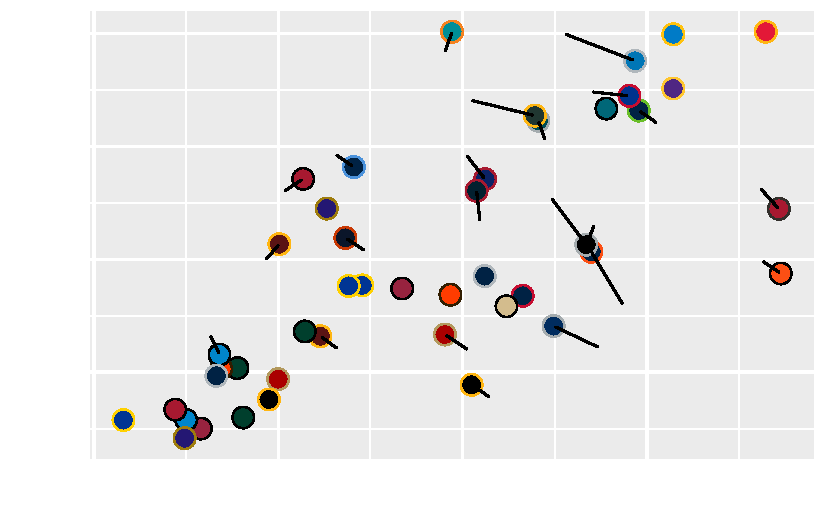
\includegraphics{04-nfl-analytics-visualization_files/figure-pdf/add-ggrepel-options-1.pdf}

}

\end{figure}

The plot, as is, is understandable in that we are able to associate each
point with a specific quarterback to examine how a quarterback's total
passing yardage is split between play action and non-play action passes.
While the graph could hypothetically ``standalone'' as is - minus a need
for a title - we can still do work on it to make it more presentable.
Let's return to our data visualization ``to do list.''

\begin{tcolorbox}[enhanced jigsaw, left=2mm, toprule=.15mm, opacitybacktitle=0.6, leftrule=.75mm, bottomrule=.15mm, colbacktitle=quarto-callout-note-color!10!white, breakable, colback=white, bottomtitle=1mm, toptitle=1mm, title=\textcolor{quarto-callout-note-color}{\faInfo}\hspace{0.5em}{Note}, coltitle=black, titlerule=0mm, arc=.35mm, opacityback=0, colframe=quarto-callout-note-color-frame, rightrule=.15mm]

Our data visualization ``to do list'':

\begin{enumerate}
\def\labelenumi{\arabic{enumi}.}
\item
  \st{Adding team colors to each point.}
\item
  \st{Increasing the size of each point.}
\item
  \st{Adding player names to each point.}
\item
  Increasing the number of ticks on each axis.
\item
  Provide the numeric values in correct format (that is, including a ,
  to correctly show thousands).
\item
  Rename the title of each axis.
\item
  Provide a title, subtitle, and caption for the plot.
\item
  Add mean lines to both x-axis and y-axis.
\item
  Change \texttt{theme} elements to make data viz more appealing.
\end{enumerate}

\end{tcolorbox}

\hypertarget{editing-axis-ticks-and-values}{%
\subsection{Editing Axis Ticks and
Values}\label{editing-axis-ticks-and-values}}

Because steps 4 and 5 from the above ``to do list'' can be accomplished
with the same package, we will lump both together and complete them at
once.

Let's first examine the idea of increasing the number of ticks on each
axis. The ``axis ticks'' refer to the specific spots on each axis
wherein a numeric data point resides. With our current visualization, we
currently have ``1000, 2000, 3000'' on the x-axis and ``400, 800, 1200,
1600'' on the y-axis.

We may want to increase the number of axis ticks in this visualization
as it can provide a more detailed view of the data being presented.
Typically, increasing the number of tickets will show more granularity
in the data and make it easier to interpret the values represented by
each point. In this specific case, we can look at the cluster of points
represented by Andy Dalton, Mac Jones, and Matt Ryan. Given the current
structure of the axis ticks, we can guess that Matt Ryan has roughly
2,500 yards on non-play action passing attempts. Given we know Matt
Ryan's amount, we can make guesses that Andy Dalton may be around 2,300
and Mac Jones somewhere between the two.

By increasing the number of values on each axis, we have the ability to
see more specific results. Conversely, we must be careful to not add too
many so that the data becomes overwhelming to interpret. Much like the
size of \texttt{geom\_point} was a case of trial and error, so is
selecting an appropriate amount of ticks.

However, before implementing these changes, we need to segue into a
discussion on continuous and discrete data.

\begin{tcolorbox}[enhanced jigsaw, left=2mm, toprule=.15mm, opacitybacktitle=0.6, leftrule=.75mm, bottomrule=.15mm, colbacktitle=quarto-callout-important-color!10!white, breakable, colback=white, bottomtitle=1mm, toptitle=1mm, title=\textcolor{quarto-callout-important-color}{\faExclamation}\hspace{0.5em}{Important}, coltitle=black, titlerule=0mm, arc=.35mm, opacityback=0, colframe=quarto-callout-important-color-frame, rightrule=.15mm]

When implementing changes to either the x- or y-axis in \texttt{ggplot},
you will be working with either continuous or discrete data, and using
the \texttt{scale\_x\_continuous} or \texttt{scale\_x\_discrete}
functions (or replacing \texttt{x} with \texttt{y} when working with the
opposite axis). In either case, both functions allow you to customize
the axis of a plot but are used for different types of data.

\texttt{scale\_x\_continuous} is used for continuous (or numeric) data,
where the axis is represented by a continuous range of numeric values.
The values within a continuous axis can take on any number within the
given range.

\texttt{scale\_x\_discrete} is used for discrete data (or often
character-based data). You will see this function used when working with
variables such as player names, teams, college names, etc. In any case,
discrete data is limited to a specific set of categories.

Please know that \texttt{ggplot} will throw an error if you try to apply
a continuous scale to discrete data, or the opposite, that reads:
\texttt{Error:\ Discrete\ value\ supplied\ to\ continuous\ scale}.

\end{tcolorbox}

In the case of our current plot, we now know we will be using the
\texttt{scales\_x\_continuous} and \texttt{scale\_y\_continuous}
functions as both contain continuous (numeric) data. To make the
changes, we can turn to the \texttt{scales} package and its
\texttt{pretty\_breaks} function to change the number of ``breaks'' (or
ticks) on each axis. By placing \texttt{n\ =\ 6} within the
\texttt{pretty\_breaks} argument, we are requesting a total of six axis
ticks on both the x- and y-axis.

\begin{Shaded}
\begin{Highlighting}[]
\FunctionTok{ggplot}\NormalTok{(}\AttributeTok{data =}\NormalTok{ play\_action\_data, }\FunctionTok{aes}\NormalTok{(}\AttributeTok{x =}\NormalTok{ yds, }\AttributeTok{y =}\NormalTok{ pa\_yds)) }\SpecialCharTok{+}
  \FunctionTok{geom\_point}\NormalTok{(}\AttributeTok{shape =} \DecValTok{21}\NormalTok{,}
             \AttributeTok{fill =}\NormalTok{ play\_action\_data}\SpecialCharTok{$}\NormalTok{team\_color,}
             \AttributeTok{color =}\NormalTok{ play\_action\_data}\SpecialCharTok{$}\NormalTok{team\_color2,}
             \AttributeTok{size =} \FloatTok{4.5}\NormalTok{) }\SpecialCharTok{+}
  \FunctionTok{geom\_text\_repel}\NormalTok{(}\FunctionTok{aes}\NormalTok{(}\AttributeTok{label =}\NormalTok{ player),}
                  \AttributeTok{box.padding =} \FloatTok{0.45}\NormalTok{,}
                  \AttributeTok{size =} \DecValTok{3}\NormalTok{,}
                  \AttributeTok{family =} \StringTok{"Roboto"}\NormalTok{,}
                  \AttributeTok{fontface =} \StringTok{"bold"}\NormalTok{) }\SpecialCharTok{+}
  \FunctionTok{scale\_x\_continuous}\NormalTok{(}\AttributeTok{breaks =}\NormalTok{ scales}\SpecialCharTok{::}\FunctionTok{pretty\_breaks}\NormalTok{(}\AttributeTok{n =} \DecValTok{6}\NormalTok{)) }\SpecialCharTok{+}
  \FunctionTok{scale\_y\_continuous}\NormalTok{(}\AttributeTok{breaks =}\NormalTok{ scales}\SpecialCharTok{::}\FunctionTok{pretty\_breaks}\NormalTok{(}\AttributeTok{n =} \DecValTok{6}\NormalTok{))}
\end{Highlighting}
\end{Shaded}

\begin{verbatim}
Warning: ggrepel: 11 unlabeled data points (too many overlaps). Consider
increasing max.overlaps
\end{verbatim}

\begin{figure}[H]

{\centering 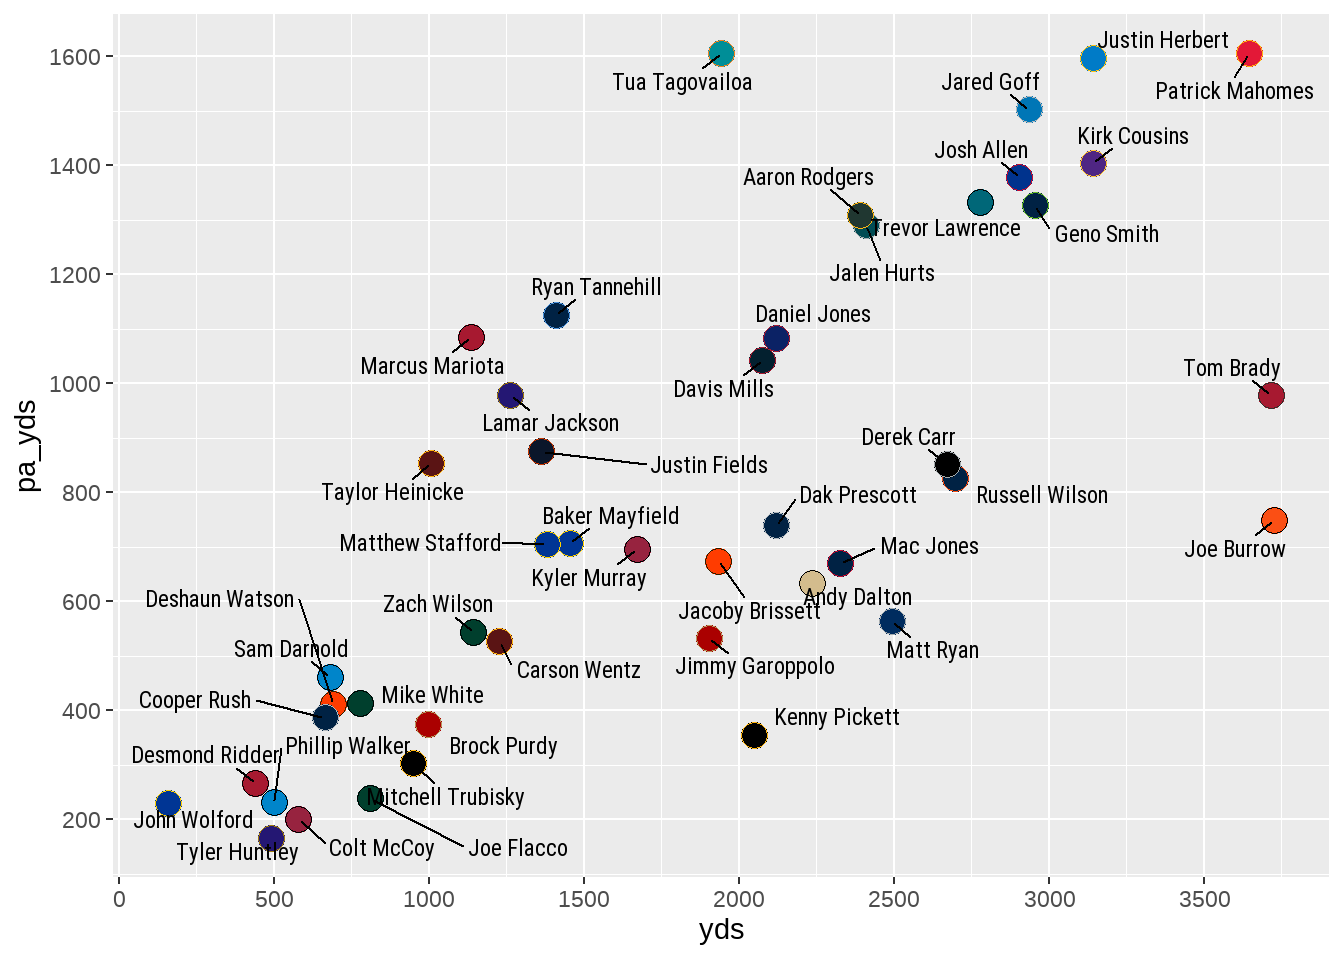
\includegraphics{04-nfl-analytics-visualization_files/figure-pdf/add-breaks-with-scales-1.pdf}

}

\end{figure}

Despite our request to build the plot with six ticks on each axis, you
will see the generated visualization includes seven on the x-axis and
eight on the y-axis. \emph{This does not mean your code with
\texttt{pretty\_breaks}} \emph{did not work}. Instead, the
\texttt{pretty\_breaks} function is designed to internally determine the
best axis tick optimization based on your requested number. To that end,
the function - ``under the hood'' - determined that seven and eight
ticks, respectively, was the most optimized way to display the data
given our desire to have at least six on each.

With the number of axis ticks corrected, we can turn our attention to
getting the labels of the axis ticks into correct numeric format. Within
the same \texttt{scale\_x\_continuous} or \texttt{scale\_y\_continuous}
arguments, we will use the \texttt{labels} function, combined with
another tool from the \texttt{scales} package to make the adjustments.

\begin{Shaded}
\begin{Highlighting}[]
\FunctionTok{ggplot}\NormalTok{(}\AttributeTok{data =}\NormalTok{ play\_action\_data, }\FunctionTok{aes}\NormalTok{(}\AttributeTok{x =}\NormalTok{ yds, }\AttributeTok{y =}\NormalTok{ pa\_yds)) }\SpecialCharTok{+}
  \FunctionTok{geom\_point}\NormalTok{(}\AttributeTok{shape =} \DecValTok{21}\NormalTok{,}
             \AttributeTok{fill =}\NormalTok{ play\_action\_data}\SpecialCharTok{$}\NormalTok{team\_color,}
             \AttributeTok{color =}\NormalTok{ play\_action\_data}\SpecialCharTok{$}\NormalTok{team\_color2,}
             \AttributeTok{size =} \FloatTok{4.5}\NormalTok{) }\SpecialCharTok{+}
  \FunctionTok{geom\_text\_repel}\NormalTok{(}\FunctionTok{aes}\NormalTok{(}\AttributeTok{label =}\NormalTok{ player),}
                  \AttributeTok{box.padding =} \FloatTok{0.45}\NormalTok{,}
                  \AttributeTok{size =} \DecValTok{3}\NormalTok{,}
                  \AttributeTok{family =} \StringTok{"Roboto"}\NormalTok{,}
                  \AttributeTok{fontface =} \StringTok{"bold"}\NormalTok{) }\SpecialCharTok{+}
  \FunctionTok{scale\_x\_continuous}\NormalTok{(}\AttributeTok{breaks =}\NormalTok{ scales}\SpecialCharTok{::}\FunctionTok{pretty\_breaks}\NormalTok{(}\AttributeTok{n =} \DecValTok{6}\NormalTok{),}
                     \AttributeTok{labels =}\NormalTok{ scales}\SpecialCharTok{::}\FunctionTok{label\_comma}\NormalTok{()) }\SpecialCharTok{+}
  \FunctionTok{scale\_y\_continuous}\NormalTok{(}\AttributeTok{breaks =}\NormalTok{ scales}\SpecialCharTok{::}\FunctionTok{pretty\_breaks}\NormalTok{(}\AttributeTok{n =} \DecValTok{6}\NormalTok{),}
                     \AttributeTok{labels =}\NormalTok{ scales}\SpecialCharTok{::}\FunctionTok{label\_comma}\NormalTok{())}
\end{Highlighting}
\end{Shaded}

\begin{verbatim}
Warning: ggrepel: 11 unlabeled data points (too many overlaps). Consider
increasing max.overlaps
\end{verbatim}

\begin{figure}[H]

{\centering 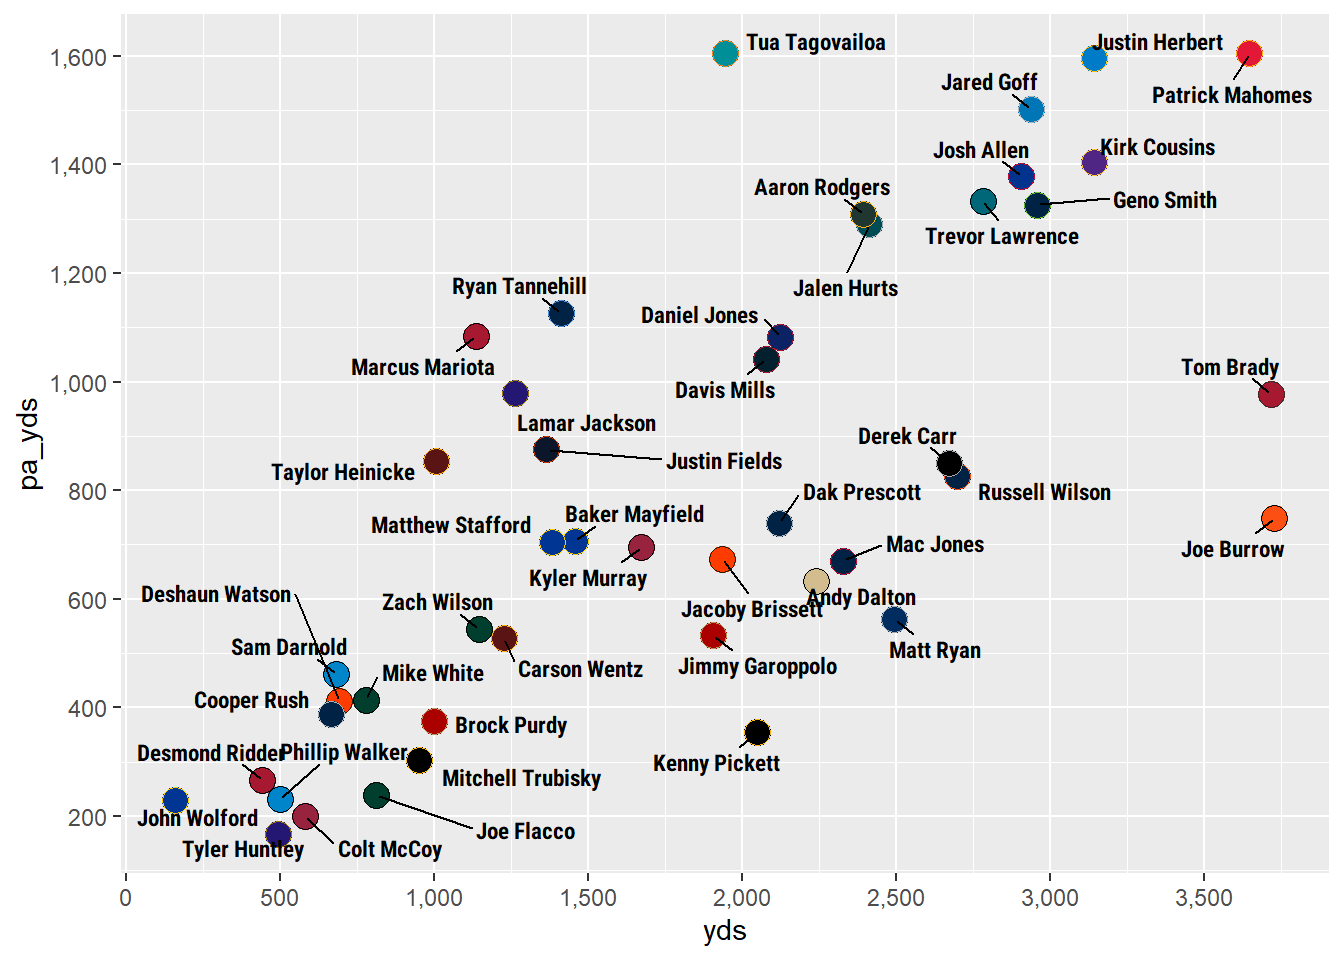
\includegraphics{04-nfl-analytics-visualization_files/figure-pdf/add-commas-to-values-1.pdf}

}

\end{figure}

By adding a \texttt{labels} option to both \texttt{scale\_x\_continuous}
and \texttt{scale\_y\_continuous}, we can use the
\texttt{label\_comma()} option from within the \texttt{scales} package
to easily add a comma into numbers that are in the thousands.

With much of the heavy lifting for our visualization now complete, we
can move on to the final steps in our ``to do list.''

\begin{tcolorbox}[enhanced jigsaw, left=2mm, toprule=.15mm, opacitybacktitle=0.6, leftrule=.75mm, bottomrule=.15mm, colbacktitle=quarto-callout-note-color!10!white, breakable, colback=white, bottomtitle=1mm, toptitle=1mm, title=\textcolor{quarto-callout-note-color}{\faInfo}\hspace{0.5em}{Note}, coltitle=black, titlerule=0mm, arc=.35mm, opacityback=0, colframe=quarto-callout-note-color-frame, rightrule=.15mm]

\textbf{Our data visualization ``to do list'':}

\begin{enumerate}
\def\labelenumi{\arabic{enumi}.}
\item
  \st{Adding team colors to each point.}
\item
  \st{Increasing the size of each point.}
\item
  \st{Adding player names to each point.}
\item
  \st{Increasing the number of ticks on each axis.}
\item
  \st{Provide the numeric values in correct format (that is, including a
  , to correctly show thousands).}
\item
  Rename the title of each axis.
\item
  Provide a title, subtitle, and caption for the plot.
\item
  Add mean lines to both x-axis and y-axis.
\item
  Change \texttt{theme} elements to make data viz more appealing.
\end{enumerate}

\end{tcolorbox}

\hypertarget{changing-axis-titles-and-adding-title-subtitle-and-caption}{%
\subsection{Changing Axis Titles and Adding Title, Subtitle, and
Caption}\label{changing-axis-titles-and-adding-title-subtitle-and-caption}}

Much like our last section, we can work on changing the title of each
axis and adding a title, subtitle, and caption for the plot within one
section, as all this is added and/or changed by using \texttt{labs()}.

\begin{Shaded}
\begin{Highlighting}[]
\FunctionTok{ggplot}\NormalTok{(}\AttributeTok{data =}\NormalTok{ play\_action\_data, }\FunctionTok{aes}\NormalTok{(}\AttributeTok{x =}\NormalTok{ yds, }\AttributeTok{y =}\NormalTok{ pa\_yds)) }\SpecialCharTok{+}
  \FunctionTok{geom\_point}\NormalTok{(}\AttributeTok{shape =} \DecValTok{21}\NormalTok{,}
             \AttributeTok{fill =}\NormalTok{ play\_action\_data}\SpecialCharTok{$}\NormalTok{team\_color,}
             \AttributeTok{color =}\NormalTok{ play\_action\_data}\SpecialCharTok{$}\NormalTok{team\_color2,}
             \AttributeTok{size =} \FloatTok{4.5}\NormalTok{) }\SpecialCharTok{+}
  \FunctionTok{geom\_text\_repel}\NormalTok{(}\FunctionTok{aes}\NormalTok{(}\AttributeTok{label =}\NormalTok{ player),}
                  \AttributeTok{box.padding =} \FloatTok{0.45}\NormalTok{,}
                  \AttributeTok{size =} \DecValTok{3}\NormalTok{,}
                  \AttributeTok{family =} \StringTok{"Roboto"}\NormalTok{,}
                  \AttributeTok{fontface =} \StringTok{"bold"}\NormalTok{) }\SpecialCharTok{+}
  \FunctionTok{scale\_x\_continuous}\NormalTok{(}\AttributeTok{breaks =}\NormalTok{ scales}\SpecialCharTok{::}\FunctionTok{pretty\_breaks}\NormalTok{(}\AttributeTok{n =} \DecValTok{6}\NormalTok{),}
                     \AttributeTok{labels =}\NormalTok{ scales}\SpecialCharTok{::}\FunctionTok{label\_comma}\NormalTok{()) }\SpecialCharTok{+}
  \FunctionTok{scale\_y\_continuous}\NormalTok{(}\AttributeTok{breaks =}\NormalTok{ scales}\SpecialCharTok{::}\FunctionTok{pretty\_breaks}\NormalTok{(}\AttributeTok{n =} \DecValTok{6}\NormalTok{),}
                     \AttributeTok{labels =}\NormalTok{ scales}\SpecialCharTok{::}\FunctionTok{label\_comma}\NormalTok{()) }\SpecialCharTok{+}
  \FunctionTok{labs}\NormalTok{(}\AttributeTok{x =} \StringTok{"Non{-}Play Action Yards"}\NormalTok{,}
       \AttributeTok{y =} \StringTok{"Play Action Yards"}\NormalTok{,}
       \AttributeTok{title =} \StringTok{"**Cumulative Passing Yards**"}\NormalTok{,}
       \AttributeTok{subtitle =} \StringTok{"*Non{-}Play Action vs. Play Action*"}\NormalTok{,}
       \AttributeTok{caption =} \StringTok{"*An Introduction to NFL Analytics with R*\textless{}br\textgreater{}**Brad J. Congelio**"}\NormalTok{)}
\end{Highlighting}
\end{Shaded}

\begin{verbatim}
Warning: ggrepel: 17 unlabeled data points (too many overlaps). Consider
increasing max.overlaps
\end{verbatim}

\begin{figure}[H]

{\centering 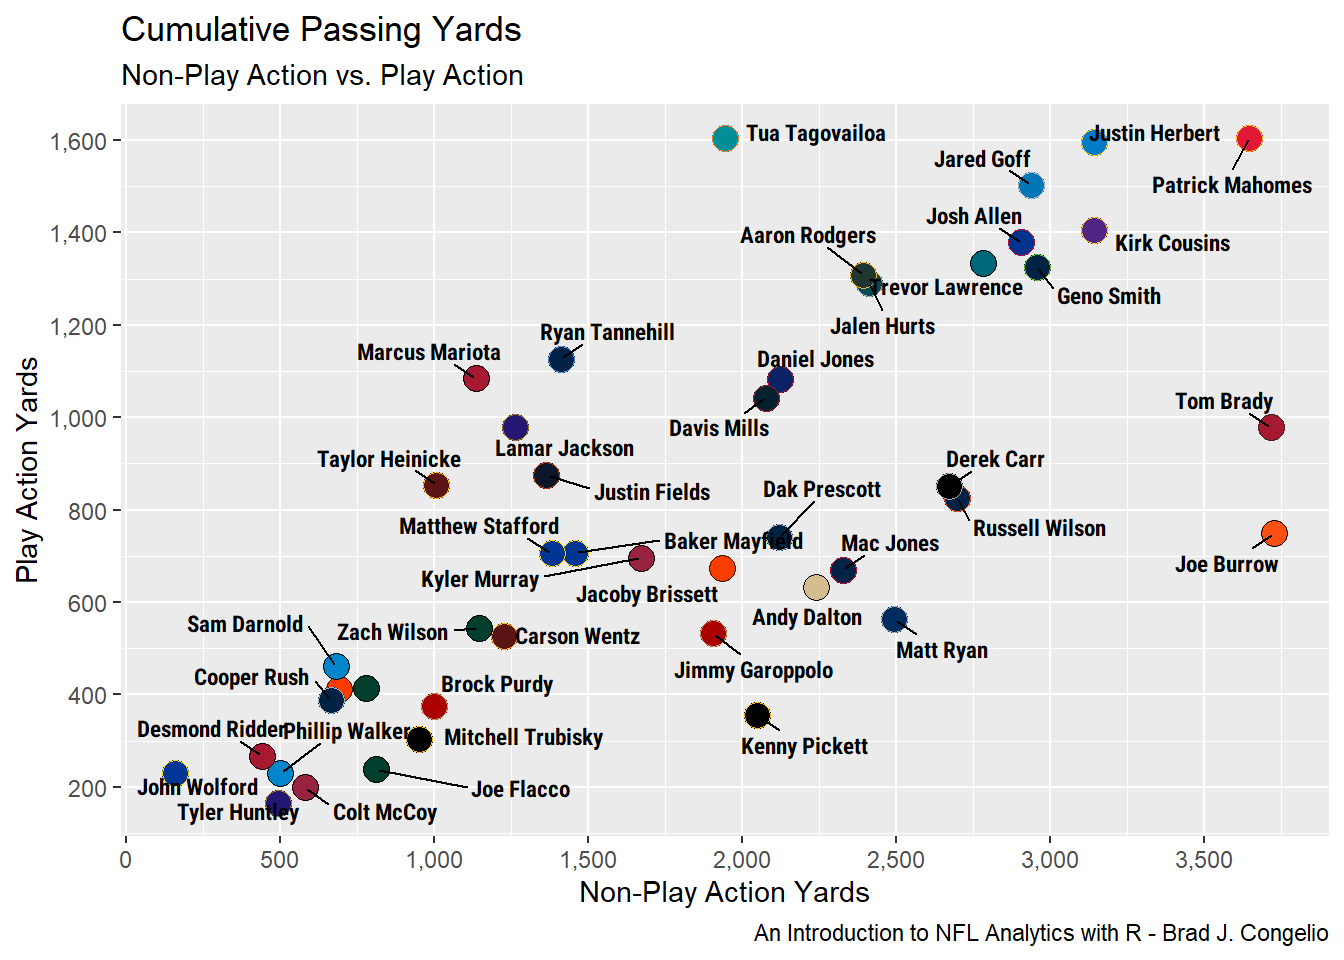
\includegraphics{04-nfl-analytics-visualization_files/figure-pdf/using-labs-for-title-caption-sub-1.pdf}

}

\end{figure}

Within the new \texttt{labs()}, we are placing a total of five items:
\texttt{x} (allowing us to name the x-axis outside the confines of what
it is called in the beginning \texttt{aes()} call, \texttt{y} (allowing
us to name the y-axis), \texttt{title} (allowing us to add a title to
the top of the plot), \texttt{subtitle} (allowing us to add a subtitle
below the title and provide more contextual information), and
\texttt{caption} (allowing us to provide information about where the
graph come from and who designed it). We will explore ways to change the
font, size, color, and more of these items when we move on to the last
item of our ``to do list.''

\begin{tcolorbox}[enhanced jigsaw, left=2mm, toprule=.15mm, opacitybacktitle=0.6, leftrule=.75mm, bottomrule=.15mm, colbacktitle=quarto-callout-note-color!10!white, breakable, colback=white, bottomtitle=1mm, toptitle=1mm, title=\textcolor{quarto-callout-note-color}{\faInfo}\hspace{0.5em}{Note}, coltitle=black, titlerule=0mm, arc=.35mm, opacityback=0, colframe=quarto-callout-note-color-frame, rightrule=.15mm]

\textbf{Our data visualization ``to do list'':}

\begin{enumerate}
\def\labelenumi{\arabic{enumi}.}
\item
  \st{Adding team colors to each point.}
\item
  \st{Increasing the size of each point.}
\item
  \st{Adding player names to each point.}
\item
  \st{Increasing the number of ticks on each axis.}
\item
  \st{Provide the numeric values in correct format (that is, including a
  , to correctly show thousands).}
\item
  \st{Rename the title of each axis.}
\item
  \st{Provide a title, subtitle, and caption for the plot.}
\item
  Add mean lines to both x-axis and y-axis.
\item
  Change theme elements to make data viz more appealing.
\end{enumerate}

\end{tcolorbox}

\hypertarget{adding-mean-lines-to-both-x-axis-and-y-axis}{%
\subsection{Adding Mean Lines to Both x-axis and
y-axis}\label{adding-mean-lines-to-both-x-axis-and-y-axis}}

Adding mean (or average) lines to both the x-axis and y-axis allows us
to visualize where each quarterback falls within one of four sections
(according to the amount of passing yards in both situations). Adding
the lines is done by add two additional geoms to the existing plot (in
this case \texttt{geom\_hline} and \texttt{geom\_vline}).

\begin{Shaded}
\begin{Highlighting}[]
\FunctionTok{ggplot}\NormalTok{(}\AttributeTok{data =}\NormalTok{ play\_action\_data, }\FunctionTok{aes}\NormalTok{(}\AttributeTok{x =}\NormalTok{ yds, }\AttributeTok{y =}\NormalTok{ pa\_yds)) }\SpecialCharTok{+}
   \FunctionTok{geom\_point}\NormalTok{(}\AttributeTok{shape =} \DecValTok{21}\NormalTok{,}
             \AttributeTok{fill =}\NormalTok{ play\_action\_data}\SpecialCharTok{$}\NormalTok{team\_color,}
             \AttributeTok{color =}\NormalTok{ play\_action\_data}\SpecialCharTok{$}\NormalTok{team\_color2,}
             \AttributeTok{size =} \FloatTok{4.5}\NormalTok{) }\SpecialCharTok{+}
  \FunctionTok{geom\_text\_repel}\NormalTok{(}\FunctionTok{aes}\NormalTok{(}\AttributeTok{label =}\NormalTok{ player),}
                  \AttributeTok{box.padding =} \FloatTok{0.45}\NormalTok{,}
                  \AttributeTok{size =} \DecValTok{3}\NormalTok{,}
                  \AttributeTok{family =} \StringTok{"Roboto"}\NormalTok{,}
                  \AttributeTok{fontface =} \StringTok{"bold"}\NormalTok{) }\SpecialCharTok{+}
  \FunctionTok{scale\_x\_continuous}\NormalTok{(}\AttributeTok{breaks =}\NormalTok{ scales}\SpecialCharTok{::}\FunctionTok{pretty\_breaks}\NormalTok{(}\AttributeTok{n =} \DecValTok{6}\NormalTok{),}
                     \AttributeTok{labels =}\NormalTok{ scales}\SpecialCharTok{::}\FunctionTok{label\_comma}\NormalTok{()) }\SpecialCharTok{+}
  \FunctionTok{scale\_y\_continuous}\NormalTok{(}\AttributeTok{breaks =}\NormalTok{ scales}\SpecialCharTok{::}\FunctionTok{pretty\_breaks}\NormalTok{(}\AttributeTok{n =} \DecValTok{6}\NormalTok{),}
                     \AttributeTok{labels =}\NormalTok{ scales}\SpecialCharTok{::}\FunctionTok{label\_comma}\NormalTok{()) }\SpecialCharTok{+}
  \FunctionTok{labs}\NormalTok{(}\AttributeTok{x =} \StringTok{"Non{-}Play Action Yards"}\NormalTok{,}
       \AttributeTok{y =} \StringTok{"Play Action Yards"}\NormalTok{,}
       \AttributeTok{title =} \StringTok{"**Cumulative Passing Yards**"}\NormalTok{,}
       \AttributeTok{subtitle =} \StringTok{"*Non{-}Play Action vs. Play Action*"}\NormalTok{,}
       \AttributeTok{caption =} \StringTok{"*An Introduction to NFL Analytics with R*\textless{}br\textgreater{}**Brad J. Congelio**"}\NormalTok{) }\SpecialCharTok{+}
  \FunctionTok{geom\_hline}\NormalTok{(}\AttributeTok{yintercept =} \FunctionTok{mean}\NormalTok{(play\_action\_data}\SpecialCharTok{$}\NormalTok{pa\_yds), }\AttributeTok{linewidth =}\NormalTok{ .}\DecValTok{8}\NormalTok{, }\AttributeTok{color =} \StringTok{"black"}\NormalTok{, }\AttributeTok{linetype =} \StringTok{"dashed"}\NormalTok{) }\SpecialCharTok{+}
  \FunctionTok{geom\_vline}\NormalTok{(}\AttributeTok{xintercept =} \FunctionTok{mean}\NormalTok{(play\_action\_data}\SpecialCharTok{$}\NormalTok{yds), }\AttributeTok{linewidth =}\NormalTok{ .}\DecValTok{8}\NormalTok{, }\AttributeTok{color =} \StringTok{"black"}\NormalTok{, }\AttributeTok{linetype =} \StringTok{"dashed"}\NormalTok{)}
\end{Highlighting}
\end{Shaded}

\begin{verbatim}
Warning: ggrepel: 17 unlabeled data points (too many overlaps). Consider
increasing max.overlaps
\end{verbatim}

\begin{figure}[H]

{\centering 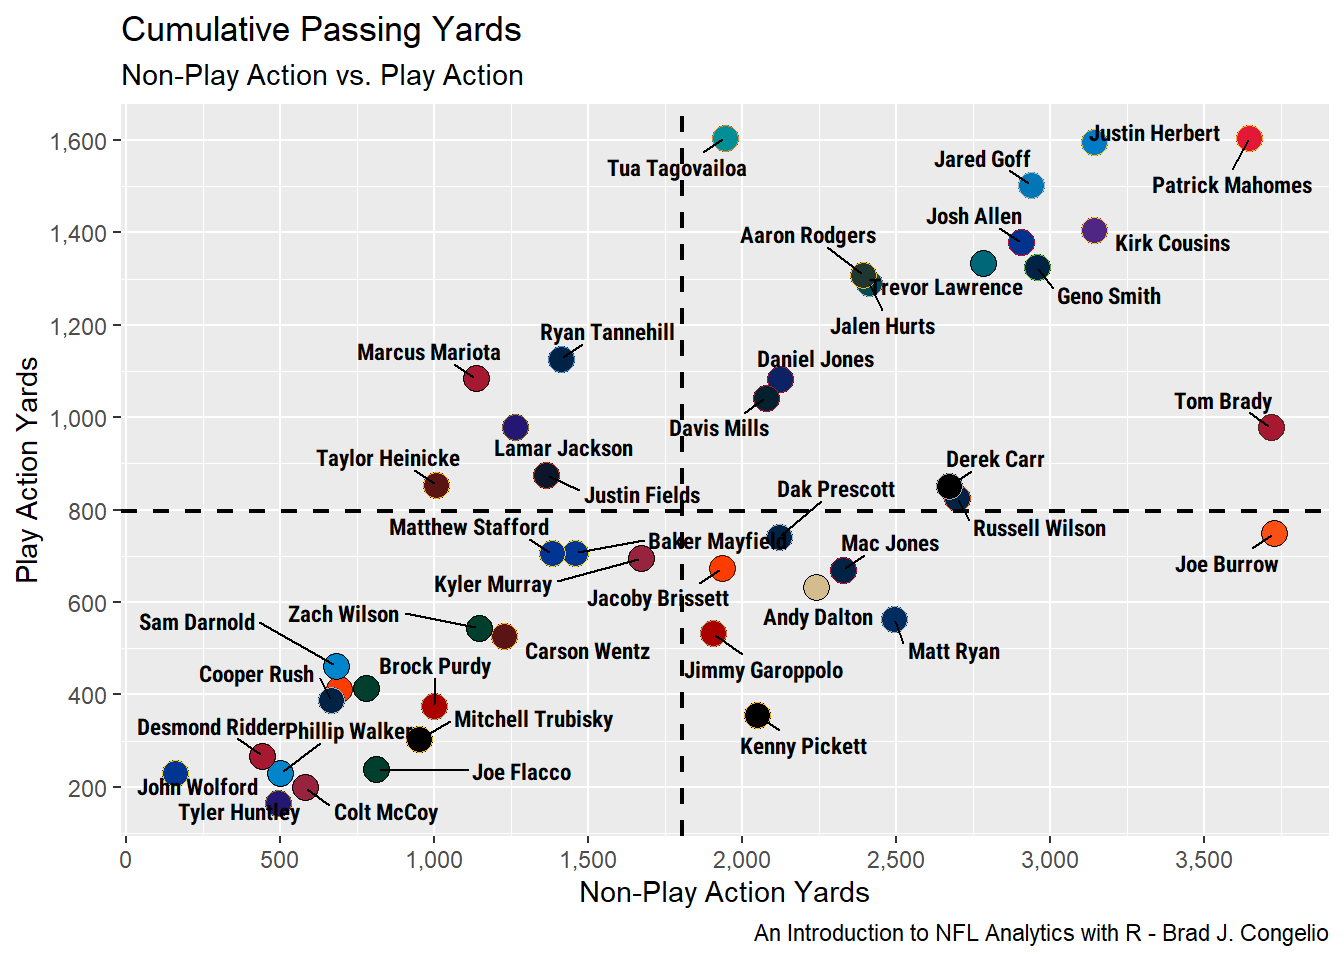
\includegraphics{04-nfl-analytics-visualization_files/figure-pdf/add-avg-lines-incorrectly-1.pdf}

}

\end{figure}

In the above output, we used \texttt{geom\_hline} and
\texttt{geom\_vline} to draw a dashed line at the average for both
\texttt{pa\_yds} at the \texttt{yintercept} and \texttt{yds} at the
\texttt{xintercept}. Because of this, we can see that - for example -
Marcus Mariota is above average for play action yards, but below average
for non-play action yards. Additionally, Matthew Stafford, Baker
Mayfield, Kyler Murray, and many others are all below average in both
metrics while Jared Goff, Justin Herbert, Patrick Mahomes, and others
are well above average in both.

However, adding the \texttt{geom\_hline} and \texttt{geom\_vline} at the
very end of the \texttt{ggplot} code creates an issues (and one I've
intentionally created for the purposes of education). As you look at the
plot, you will see that the dashed line runs \textbf{on top} of the
names and dots in the plot. This is because \texttt{ggplot} follows a
very specific ordering of layering.

\begin{tcolorbox}[enhanced jigsaw, left=2mm, toprule=.15mm, opacitybacktitle=0.6, leftrule=.75mm, bottomrule=.15mm, colbacktitle=quarto-callout-important-color!10!white, breakable, colback=white, bottomtitle=1mm, toptitle=1mm, title=\textcolor{quarto-callout-important-color}{\faExclamation}\hspace{0.5em}{Important}, coltitle=black, titlerule=0mm, arc=.35mm, opacityback=0, colframe=quarto-callout-important-color-frame, rightrule=.15mm]

In \texttt{ggplot}, it is important to remember that items in a plot are
layered in the order in which they are added to the plot. This process
of layering is important because it ultimately determines which items
end up on top of others, which can have significant implications on the
visual appearance of the plot.

As we've seen so far in the process, each layer of a plot is added by
including a \texttt{geom\_}. The first layer added will \emph{always} be
at the very bottom of the plot, with each additional layer building on
top of the previous layers.

\end{tcolorbox}

Because of the important layering issue highlighted above, it is
visually necessary for us to move the \texttt{geom\_hline} and
\texttt{geom\_vline} to the beginning of the \texttt{ggplot} code so
both are layered underneath everything else in the plot
(\texttt{geom\_point} and \texttt{geom\_text\_repel} in this case). As
well, we can apply the \texttt{alpha} option to each to slightly
decrease each line's transparency.

\begin{Shaded}
\begin{Highlighting}[]
\FunctionTok{ggplot}\NormalTok{(}\AttributeTok{data =}\NormalTok{ play\_action\_data, }\FunctionTok{aes}\NormalTok{(}\AttributeTok{x =}\NormalTok{ yds, }\AttributeTok{y =}\NormalTok{ pa\_yds)) }\SpecialCharTok{+}
  \FunctionTok{geom\_hline}\NormalTok{(}\AttributeTok{yintercept =} \FunctionTok{mean}\NormalTok{(play\_action\_data}\SpecialCharTok{$}\NormalTok{pa\_yds), }
             \AttributeTok{linewidth =}\NormalTok{ .}\DecValTok{8}\NormalTok{, }
             \AttributeTok{color =} \StringTok{"black"}\NormalTok{, }
             \AttributeTok{linetype =} \StringTok{"dashed"}\NormalTok{,}
             \AttributeTok{alpha =} \FloatTok{0.5}\NormalTok{) }\SpecialCharTok{+}
  \FunctionTok{geom\_vline}\NormalTok{(}\AttributeTok{xintercept =} \FunctionTok{mean}\NormalTok{(play\_action\_data}\SpecialCharTok{$}\NormalTok{yds), }
             \AttributeTok{linewidth =}\NormalTok{ .}\DecValTok{8}\NormalTok{, }
             \AttributeTok{color =} \StringTok{"black"}\NormalTok{, }
             \AttributeTok{linetype =} \StringTok{"dashed"}\NormalTok{,}
             \AttributeTok{alpha =} \FloatTok{0.5}\NormalTok{) }\SpecialCharTok{+}
   \FunctionTok{geom\_point}\NormalTok{(}\AttributeTok{shape =} \DecValTok{21}\NormalTok{,}
             \AttributeTok{fill =}\NormalTok{ play\_action\_data}\SpecialCharTok{$}\NormalTok{team\_color,}
             \AttributeTok{color =}\NormalTok{ play\_action\_data}\SpecialCharTok{$}\NormalTok{team\_color2,}
             \AttributeTok{size =} \FloatTok{4.5}\NormalTok{) }\SpecialCharTok{+}
  \FunctionTok{geom\_text\_repel}\NormalTok{(}\FunctionTok{aes}\NormalTok{(}\AttributeTok{label =}\NormalTok{ player),}
                  \AttributeTok{box.padding =} \FloatTok{0.45}\NormalTok{,}
                  \AttributeTok{size =} \DecValTok{3}\NormalTok{,}
                  \AttributeTok{family =} \StringTok{"Roboto"}\NormalTok{,}
                  \AttributeTok{fontface =} \StringTok{"bold"}\NormalTok{) }\SpecialCharTok{+}
  \FunctionTok{scale\_x\_continuous}\NormalTok{(}\AttributeTok{breaks =}\NormalTok{ scales}\SpecialCharTok{::}\FunctionTok{pretty\_breaks}\NormalTok{(}\AttributeTok{n =} \DecValTok{6}\NormalTok{),}
                     \AttributeTok{labels =}\NormalTok{ scales}\SpecialCharTok{::}\FunctionTok{label\_comma}\NormalTok{()) }\SpecialCharTok{+}
  \FunctionTok{scale\_y\_continuous}\NormalTok{(}\AttributeTok{breaks =}\NormalTok{ scales}\SpecialCharTok{::}\FunctionTok{pretty\_breaks}\NormalTok{(}\AttributeTok{n =} \DecValTok{6}\NormalTok{),}
                     \AttributeTok{labels =}\NormalTok{ scales}\SpecialCharTok{::}\FunctionTok{label\_comma}\NormalTok{()) }\SpecialCharTok{+}
  \FunctionTok{labs}\NormalTok{(}\AttributeTok{x =} \StringTok{"Non{-}Play Action Yards"}\NormalTok{,}
       \AttributeTok{y =} \StringTok{"Play Action Yards"}\NormalTok{,}
       \AttributeTok{title =} \StringTok{"**Cumulative Passing Yards**"}\NormalTok{,}
       \AttributeTok{subtitle =} \StringTok{"*Non{-}Play Action vs. Play Action*"}\NormalTok{,}
       \AttributeTok{caption =} \StringTok{"*An Introduction to NFL Analytics with R*\textless{}br\textgreater{}**Brad J. Congelio**"}\NormalTok{)}
\end{Highlighting}
\end{Shaded}

\begin{verbatim}
Warning: ggrepel: 17 unlabeled data points (too many overlaps). Consider
increasing max.overlaps
\end{verbatim}

\begin{figure}[H]

{\centering 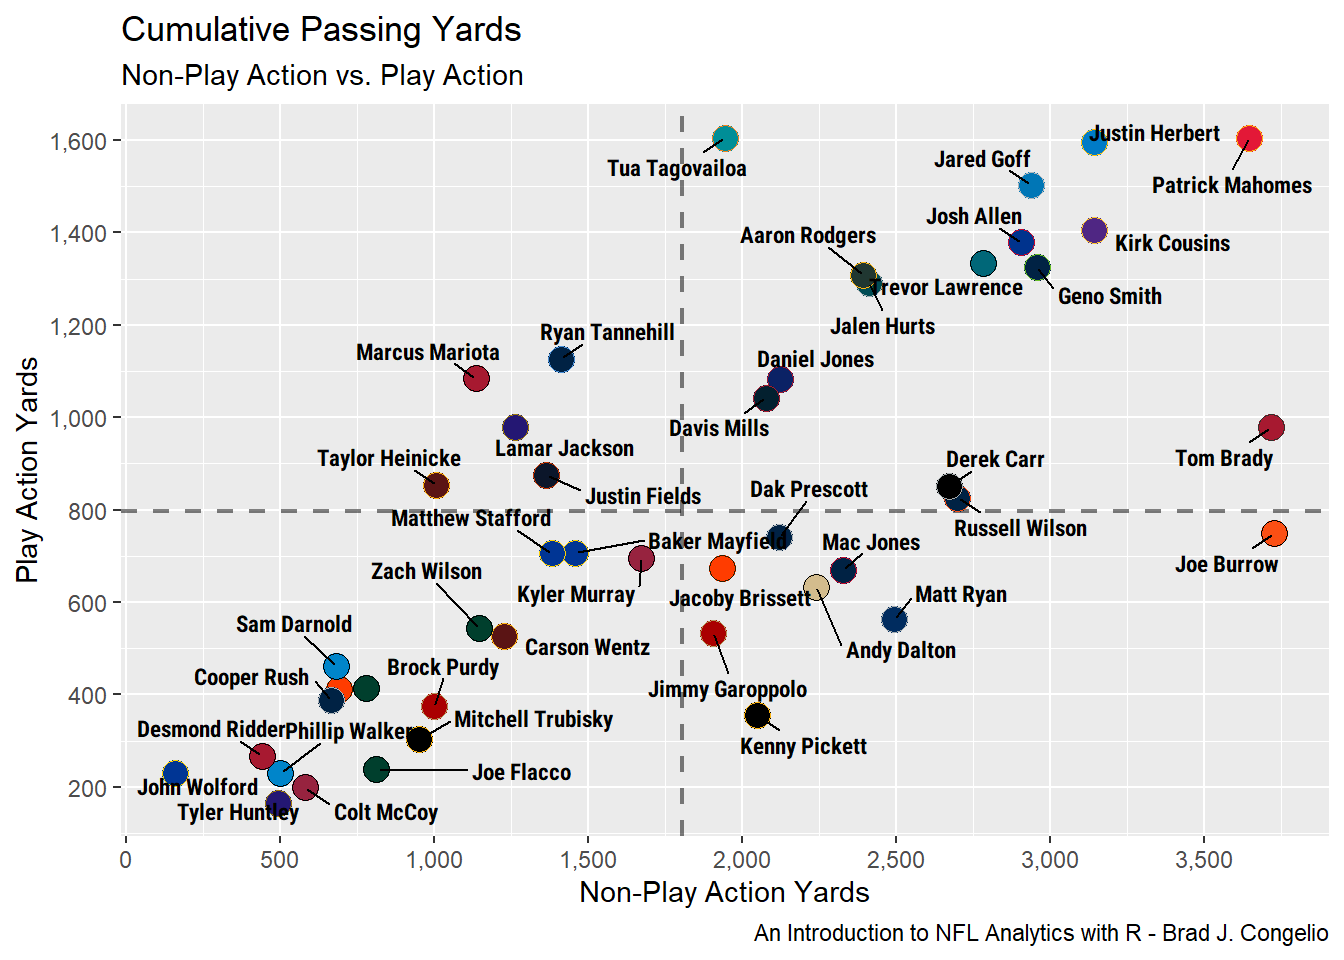
\includegraphics{04-nfl-analytics-visualization_files/figure-pdf/correctly-adding-avg-lines-1.pdf}

}

\end{figure}

By moving the average lines to the top of our \texttt{ggplot} code, both
are now layered under the other two \texttt{geom\_} and are not visually
impacting the final plot.

\hypertarget{adding-mean-lines-with-nflplotr}{%
\subsubsection{\texorpdfstring{Adding Mean Lines with
\texttt{nflplotR}}{Adding Mean Lines with nflplotR}}\label{adding-mean-lines-with-nflplotr}}

\begin{tcolorbox}[enhanced jigsaw, left=2mm, toprule=.15mm, opacitybacktitle=0.6, leftrule=.75mm, bottomrule=.15mm, colbacktitle=quarto-callout-tip-color!10!white, breakable, colback=white, bottomtitle=1mm, toptitle=1mm, title=\textcolor{quarto-callout-tip-color}{\faLightbulb}\hspace{0.5em}{Tip}, coltitle=black, titlerule=0mm, arc=.35mm, opacityback=0, colframe=quarto-callout-tip-color-frame, rightrule=.15mm]

Even though we were not able to use \texttt{nflplotR} to handle the
colors in this plot because the data lacked a corresponding
\texttt{team\_abbr} variable, we can still use \texttt{nflplotR} to add
our mean lines - and I actually recommend doing so, as it requires less
lines of code (thus less typing). See below for an example.

\end{tcolorbox}

\begin{Shaded}
\begin{Highlighting}[]
\FunctionTok{ggplot}\NormalTok{(}\AttributeTok{data =}\NormalTok{ play\_action\_data, }\FunctionTok{aes}\NormalTok{(}\AttributeTok{x =}\NormalTok{ yds, }\AttributeTok{y =}\NormalTok{ pa\_yds)) }\SpecialCharTok{+}
  \FunctionTok{geom\_mean\_lines}\NormalTok{(}\FunctionTok{aes}\NormalTok{(}\AttributeTok{v\_var =}\NormalTok{ yds, }\AttributeTok{h\_var =}\NormalTok{ pa\_yds), }
                  \AttributeTok{size =} \FloatTok{0.8}\NormalTok{,}
                  \AttributeTok{color =} \StringTok{"black"}\NormalTok{, }
                  \AttributeTok{linetype =} \StringTok{"dashed"}\NormalTok{,}
                  \AttributeTok{alpha =} \FloatTok{0.5}\NormalTok{) }\SpecialCharTok{+}
  \FunctionTok{geom\_point}\NormalTok{(}\AttributeTok{shape =} \DecValTok{21}\NormalTok{,}
             \AttributeTok{fill =}\NormalTok{ play\_action\_data}\SpecialCharTok{$}\NormalTok{team\_color,}
             \AttributeTok{color =}\NormalTok{ play\_action\_data}\SpecialCharTok{$}\NormalTok{team\_color2,}
             \AttributeTok{size =} \FloatTok{4.5}\NormalTok{) }\SpecialCharTok{+}
  \FunctionTok{geom\_text\_repel}\NormalTok{(}\FunctionTok{aes}\NormalTok{(}\AttributeTok{label =}\NormalTok{ player),}
                  \AttributeTok{box.padding =} \FloatTok{0.45}\NormalTok{,}
                  \AttributeTok{size =} \DecValTok{3}\NormalTok{,}
                  \AttributeTok{family =} \StringTok{"Roboto"}\NormalTok{,}
                  \AttributeTok{fontface =} \StringTok{"bold"}\NormalTok{) }\SpecialCharTok{+}
  \FunctionTok{scale\_x\_continuous}\NormalTok{(}\AttributeTok{breaks =}\NormalTok{ scales}\SpecialCharTok{::}\FunctionTok{pretty\_breaks}\NormalTok{(}\AttributeTok{n =} \DecValTok{6}\NormalTok{),}
                     \AttributeTok{labels =}\NormalTok{ scales}\SpecialCharTok{::}\FunctionTok{label\_comma}\NormalTok{()) }\SpecialCharTok{+}
  \FunctionTok{scale\_y\_continuous}\NormalTok{(}\AttributeTok{breaks =}\NormalTok{ scales}\SpecialCharTok{::}\FunctionTok{pretty\_breaks}\NormalTok{(}\AttributeTok{n =} \DecValTok{6}\NormalTok{),}
                     \AttributeTok{labels =}\NormalTok{ scales}\SpecialCharTok{::}\FunctionTok{label\_comma}\NormalTok{()) }\SpecialCharTok{+}
  \FunctionTok{labs}\NormalTok{(}\AttributeTok{x =} \StringTok{"Non{-}Play Action Yards"}\NormalTok{,}
       \AttributeTok{y =} \StringTok{"Play Action Yards"}\NormalTok{,}
       \AttributeTok{title =} \StringTok{"**Cumulative Passing Yards**"}\NormalTok{,}
       \AttributeTok{subtitle =} \StringTok{"*Non{-}Play Action vs. Play Action*"}\NormalTok{,}
       \AttributeTok{caption =} \StringTok{"*An Introduction to NFL Analytics with R*\textless{}br\textgreater{}**Brad J. Congelio**"}\NormalTok{)}
\end{Highlighting}
\end{Shaded}

\begin{verbatim}
Warning: Using the `size` aesthetic with geom_segment was deprecated in ggplot2 3.4.0.
i Please use the `linewidth` aesthetic instead.
\end{verbatim}

\begin{verbatim}
Warning: ggrepel: 17 unlabeled data points (too many overlaps). Consider
increasing max.overlaps
\end{verbatim}

\begin{figure}[H]

{\centering 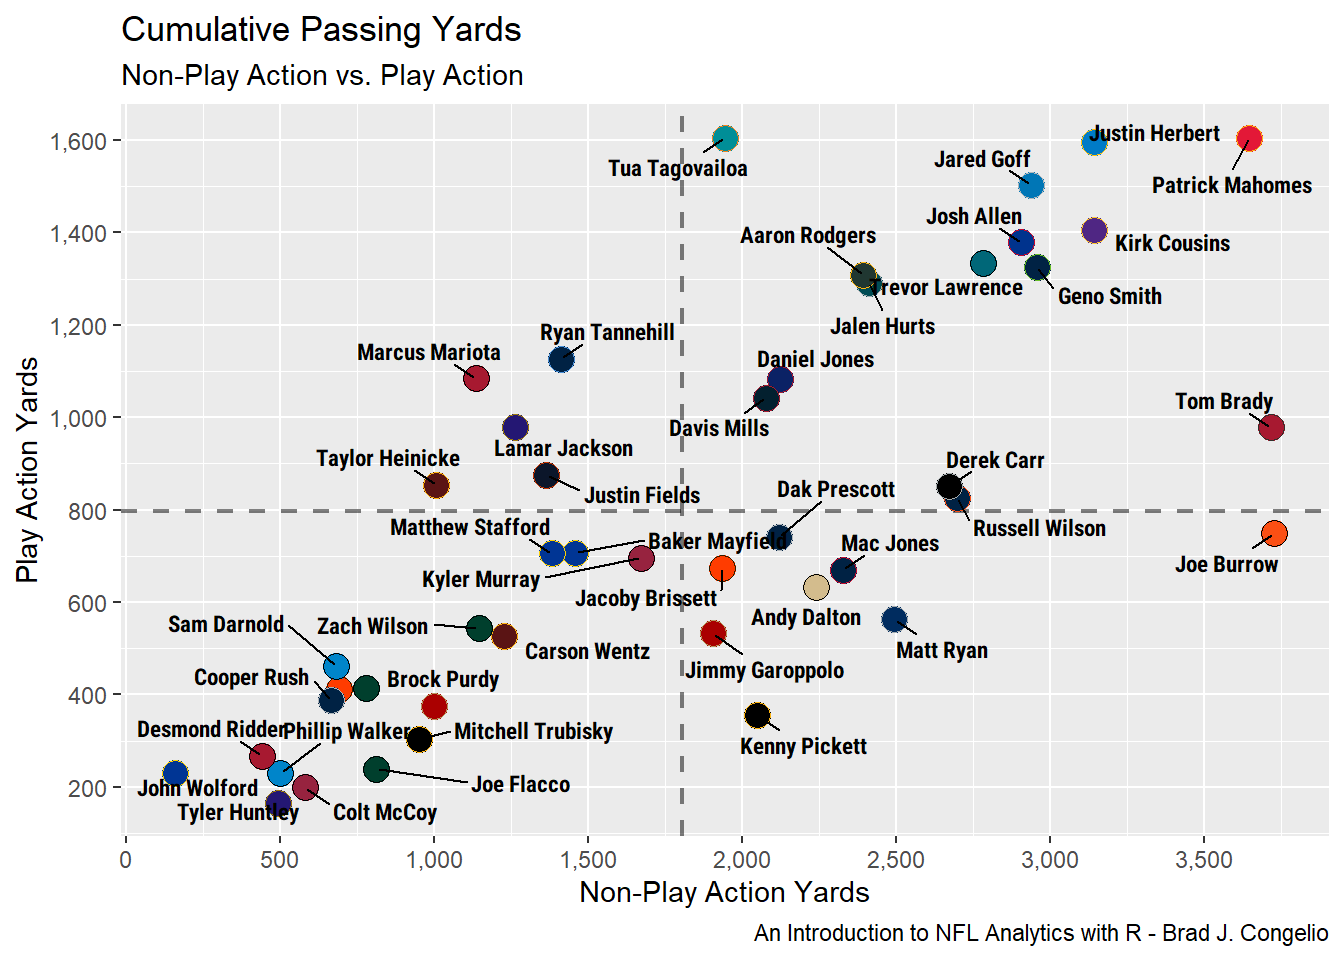
\includegraphics{04-nfl-analytics-visualization_files/figure-pdf/mean-lines-with-nflplotr-1.pdf}

}

\end{figure}

By using the \texttt{geom\_mean\_lines()} function within
\texttt{nflplotR}, we can construct both of the lines together rather
than needing to provide a \texttt{geom\_hline()} and a
\texttt{geom\_vline()} argument. Because of this, we can also provide
the size, width, and type of our line just once (rather than repeating
it again like we had to in the former method).

We can now move onto the final item on our data visualization ``to do
list.''

\begin{tcolorbox}[enhanced jigsaw, left=2mm, toprule=.15mm, opacitybacktitle=0.6, leftrule=.75mm, bottomrule=.15mm, colbacktitle=quarto-callout-note-color!10!white, breakable, colback=white, bottomtitle=1mm, toptitle=1mm, title=\textcolor{quarto-callout-note-color}{\faInfo}\hspace{0.5em}{Note}, coltitle=black, titlerule=0mm, arc=.35mm, opacityback=0, colframe=quarto-callout-note-color-frame, rightrule=.15mm]

\textbf{Our data visualization ``to do list'':}

\begin{enumerate}
\def\labelenumi{\arabic{enumi}.}
\item
  \st{Adding team colors to each point.}
\item
  \st{Increasing the size of each point.}
\item
  \st{Adding player names to each point.}
\item
  \st{Increasing the number of ticks on each axis.}
\item
  \st{Provide the numeric values in correct format (that is, including a
  , to correctly show thousands).}
\item
  \st{Rename the title of each axis.}
\item
  \st{Provide a title, subtitle, and caption for the plot.}
\item
  \st{Add mean lines to both x-axis and y-axis.}
\item
  Change theme elements to make data viz more appealing.
\end{enumerate}

\end{tcolorbox}

\hypertarget{making-changes-to-theme-elements}{%
\subsection{Making Changes to Theme
Elements}\label{making-changes-to-theme-elements}}

There is a laundry list of options to be explored when it comes to
editing your plot's theme elements to make it look exactly as you want.
Currently, according to the \texttt{ggplot2} website, the following is a
comprehensive list of elements that you can tinker with.

\begin{Shaded}
\begin{Highlighting}[]
\NormalTok{  line,}
\NormalTok{  rect,}
\NormalTok{  text,}
\NormalTok{  title,}
\NormalTok{  aspect.ratio,}
\NormalTok{  axis.title,}
\NormalTok{  axis.title.x,}
\NormalTok{  axis.title.x.top,}
\NormalTok{  axis.title.x.bottom,}
\NormalTok{  axis.title.y,}
\NormalTok{  axis.title.y.left,}
\NormalTok{  axis.title.y.right,}
\NormalTok{  axis.text,}
\NormalTok{  axis.text.x,}
\NormalTok{  axis.text.x.top,}
\NormalTok{  axis.text.x.bottom,}
\NormalTok{  axis.text.y,}
\NormalTok{  axis.text.y.left,}
\NormalTok{  axis.text.y.right,}
\NormalTok{  axis.ticks,}
\NormalTok{  axis.ticks.x,}
\NormalTok{  axis.ticks.x.top,}
\NormalTok{  axis.ticks.x.bottom,}
\NormalTok{  axis.ticks.y,}
\NormalTok{  axis.ticks.y.left,}
\NormalTok{  axis.ticks.y.right,}
\NormalTok{  axis.ticks.length,}
\NormalTok{  axis.ticks.length.x,}
\NormalTok{  axis.ticks.length.x.top,}
\NormalTok{  axis.ticks.length.x.bottom,}
\NormalTok{  axis.ticks.length.y,}
\NormalTok{  axis.ticks.length.y.left,}
\NormalTok{  axis.ticks.length.y.right,}
\NormalTok{  axis.line,}
\NormalTok{  axis.line.x,}
\NormalTok{  axis.line.x.top,}
\NormalTok{  axis.line.x.bottom,}
\NormalTok{  axis.line.y,}
\NormalTok{  axis.line.y.left,}
\NormalTok{  axis.line.y.right,}
\NormalTok{  legend.background,}
\NormalTok{  legend.margin,}
\NormalTok{  legend.spacing,}
\NormalTok{  legend.spacing.x,}
\NormalTok{  legend.spacing.y,}
\NormalTok{  legend.key,}
\NormalTok{  legend.key.size,}
\NormalTok{  legend.key.height,}
\NormalTok{  legend.key.width,}
\NormalTok{  legend.text,}
\NormalTok{  legend.text.align,}
\NormalTok{  legend.title,}
\NormalTok{  legend.title.align,}
\NormalTok{  legend.position,}
\NormalTok{  legend.direction,}
\NormalTok{  legend.justification,}
\NormalTok{  legend.box,}
\NormalTok{  legend.box.just,}
\NormalTok{  legend.box.margin,}
\NormalTok{  legend.box.background,}
\NormalTok{  legend.box.spacing,}
\NormalTok{  panel.background,}
\NormalTok{  panel.border,}
\NormalTok{  panel.spacing,}
\NormalTok{  panel.spacing.x,}
\NormalTok{  panel.spacing.y,}
\NormalTok{  panel.grid,}
\NormalTok{  panel.grid.major,}
\NormalTok{  panel.grid.minor,}
\NormalTok{  panel.grid.major.x,}
\NormalTok{  panel.grid.major.y,}
\NormalTok{  panel.grid.minor.x,}
\NormalTok{  panel.grid.minor.y,}
\NormalTok{  panel.ontop,}
\NormalTok{  plot.background,}
\NormalTok{  plot.title,}
\NormalTok{  plot.title.position,}
\NormalTok{  plot.subtitle,}
\NormalTok{  plot.caption,}
\NormalTok{  plot.caption.position,}
\NormalTok{  plot.tag,}
\NormalTok{  plot.tag.position,}
\NormalTok{  plot.margin,}
\NormalTok{  strip.background,}
\NormalTok{  strip.background.x,}
\NormalTok{  strip.background.y,}
\NormalTok{  strip.clip,}
\NormalTok{  strip.placement,}
\NormalTok{  strip.text,}
\NormalTok{  strip.text.x,}
\NormalTok{  strip.text.x.bottom,}
\NormalTok{  strip.text.x.top,}
\NormalTok{  strip.text.y,}
\NormalTok{  strip.text.y.left,}
\NormalTok{  strip.text.y.right,}
\NormalTok{  strip.switch.pad.grid,}
\NormalTok{  strip.switch.pad.wrap}
\end{Highlighting}
\end{Shaded}

It's not likely that we will encounter all these theme elements in this
book. But, the ones we do use, we will use heavily. For example, I
prefer to design all of my data visualizations without the ``axis
ticks'' (those small lines sticking out from the plot just above, or
beside, each yardage number).

\begin{tcolorbox}[enhanced jigsaw, left=2mm, toprule=.15mm, opacitybacktitle=0.6, leftrule=.75mm, bottomrule=.15mm, colbacktitle=quarto-callout-tip-color!10!white, breakable, colback=white, bottomtitle=1mm, toptitle=1mm, title=\textcolor{quarto-callout-tip-color}{\faLightbulb}\hspace{0.5em}{Tip}, coltitle=black, titlerule=0mm, arc=.35mm, opacityback=0, colframe=quarto-callout-tip-color-frame, rightrule=.15mm]

Please note the keywords in the above paragraph: ``\textbf{I prefer.''}

Nearly all the work you conduct within the \texttt{theme()} of your data
visualizations are just that - your preference. I very much have a
``personal preference'' that unites all the data viz work that I do and
share for public consumption.

You can feel free to follow along with my preferences, including the use
of the upcoming \texttt{nfl\_analytics\_theme()} I will provide, or to
make slight (or major!) adjustments to everything we cover in the coming
section to make it fit your artistic vision.

Be creative and do not be afraid to experiment with all the options
available to you in \texttt{theme()}.

\end{tcolorbox}

Let's start by removing the ticks on both the x- and y-axis. To do so,
we will add the \texttt{theme()} argument at the end of your prior
\texttt{ggplot} code and then start building out each and every change
we want to make from the above list of options.

\begin{Shaded}
\begin{Highlighting}[]
\FunctionTok{ggplot}\NormalTok{(}\AttributeTok{data =}\NormalTok{ play\_action\_data, }\FunctionTok{aes}\NormalTok{(}\AttributeTok{x =}\NormalTok{ yds, }\AttributeTok{y =}\NormalTok{ pa\_yds)) }\SpecialCharTok{+}
  \FunctionTok{geom\_mean\_lines}\NormalTok{(}\FunctionTok{aes}\NormalTok{(}\AttributeTok{v\_var =}\NormalTok{ yds, }\AttributeTok{h\_var =}\NormalTok{ pa\_yds), }
                  \AttributeTok{size =} \FloatTok{0.8}\NormalTok{,}
                  \AttributeTok{color =} \StringTok{"black"}\NormalTok{, }
                  \AttributeTok{linetype =} \StringTok{"dashed"}\NormalTok{,}
                  \AttributeTok{alpha =} \FloatTok{0.5}\NormalTok{) }\SpecialCharTok{+}
  \FunctionTok{geom\_point}\NormalTok{(}\AttributeTok{shape =} \DecValTok{21}\NormalTok{,}
             \AttributeTok{fill =}\NormalTok{ play\_action\_data}\SpecialCharTok{$}\NormalTok{team\_color,}
             \AttributeTok{color =}\NormalTok{ play\_action\_data}\SpecialCharTok{$}\NormalTok{team\_color2,}
             \AttributeTok{size =} \FloatTok{4.5}\NormalTok{) }\SpecialCharTok{+}
  \FunctionTok{geom\_text\_repel}\NormalTok{(}\FunctionTok{aes}\NormalTok{(}\AttributeTok{label =}\NormalTok{ player),}
                  \AttributeTok{box.padding =} \FloatTok{0.45}\NormalTok{,}
                  \AttributeTok{size =} \DecValTok{3}\NormalTok{,}
                  \AttributeTok{family =} \StringTok{"Roboto"}\NormalTok{,}
                  \AttributeTok{fontface =} \StringTok{"bold"}\NormalTok{) }\SpecialCharTok{+}
  \FunctionTok{scale\_x\_continuous}\NormalTok{(}\AttributeTok{breaks =}\NormalTok{ scales}\SpecialCharTok{::}\FunctionTok{pretty\_breaks}\NormalTok{(}\AttributeTok{n =} \DecValTok{6}\NormalTok{),}
                     \AttributeTok{labels =}\NormalTok{ scales}\SpecialCharTok{::}\FunctionTok{label\_comma}\NormalTok{()) }\SpecialCharTok{+}
  \FunctionTok{scale\_y\_continuous}\NormalTok{(}\AttributeTok{breaks =}\NormalTok{ scales}\SpecialCharTok{::}\FunctionTok{pretty\_breaks}\NormalTok{(}\AttributeTok{n =} \DecValTok{6}\NormalTok{),}
                     \AttributeTok{labels =}\NormalTok{ scales}\SpecialCharTok{::}\FunctionTok{label\_comma}\NormalTok{()) }\SpecialCharTok{+}
  \FunctionTok{labs}\NormalTok{(}\AttributeTok{x =} \StringTok{"Non{-}Play Action Yards"}\NormalTok{,}
       \AttributeTok{y =} \StringTok{"Play Action Yards"}\NormalTok{,}
       \AttributeTok{title =} \StringTok{"**Cumulative Passing Yards**"}\NormalTok{,}
       \AttributeTok{subtitle =} \StringTok{"*Non{-}Play Action vs. Play Action*"}\NormalTok{,}
       \AttributeTok{caption =} \StringTok{"*An Introduction to NFL Analytics with R*\textless{}br\textgreater{}**Brad J. Congelio**"}\NormalTok{) }\SpecialCharTok{+}
  \FunctionTok{theme}\NormalTok{(}
    \AttributeTok{axis.ticks =} \FunctionTok{element\_blank}\NormalTok{())}
\end{Highlighting}
\end{Shaded}

\begin{verbatim}
Warning: ggrepel: 17 unlabeled data points (too many overlaps). Consider
increasing max.overlaps
\end{verbatim}

\begin{figure}[H]

{\centering 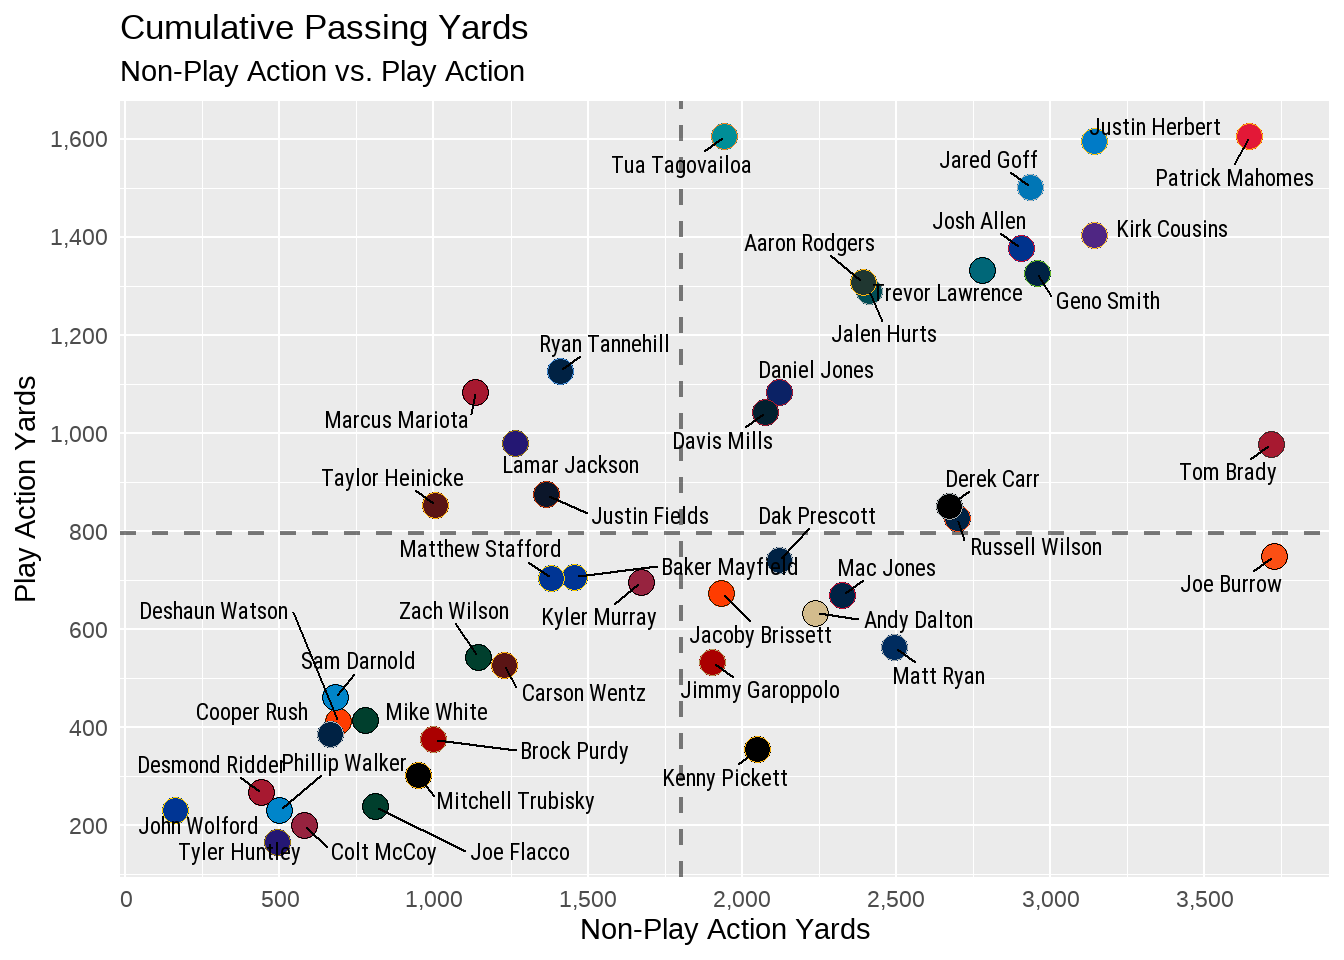
\includegraphics{04-nfl-analytics-visualization_files/figure-pdf/using-theme-to-remove-ticks-1.pdf}

}

\end{figure}

Within the \texttt{theme()} argument, as mentioned, we simply take the
specific element we wish to change (from the above list of possibilities
from the \texttt{ggplot2} website) and then provide the instruction on
what to do. In this case, since we wish to completely remove the
\texttt{axis.ticks} from the entire plot, we can provide
\texttt{element\_blank()} which removes them. We can continue making
changes to the plot's elements by adding all of these preferences to out
\texttt{theme()}.

\begin{Shaded}
\begin{Highlighting}[]
\FunctionTok{ggplot}\NormalTok{(}\AttributeTok{data =}\NormalTok{ play\_action\_data, }\FunctionTok{aes}\NormalTok{(}\AttributeTok{x =}\NormalTok{ yds, }\AttributeTok{y =}\NormalTok{ pa\_yds)) }\SpecialCharTok{+}
  \FunctionTok{geom\_mean\_lines}\NormalTok{(}\FunctionTok{aes}\NormalTok{(}\AttributeTok{v\_var =}\NormalTok{ yds, }\AttributeTok{h\_var =}\NormalTok{ pa\_yds), }
                  \AttributeTok{size =} \FloatTok{0.8}\NormalTok{,}
                  \AttributeTok{color =} \StringTok{"black"}\NormalTok{, }
                  \AttributeTok{linetype =} \StringTok{"dashed"}\NormalTok{,}
                  \AttributeTok{alpha =} \FloatTok{0.5}\NormalTok{) }\SpecialCharTok{+}
  \FunctionTok{geom\_point}\NormalTok{(}\AttributeTok{shape =} \DecValTok{21}\NormalTok{,}
             \AttributeTok{fill =}\NormalTok{ play\_action\_data}\SpecialCharTok{$}\NormalTok{team\_color,}
             \AttributeTok{color =}\NormalTok{ play\_action\_data}\SpecialCharTok{$}\NormalTok{team\_color2,}
             \AttributeTok{size =} \FloatTok{4.5}\NormalTok{) }\SpecialCharTok{+}
  \FunctionTok{geom\_text\_repel}\NormalTok{(}\FunctionTok{aes}\NormalTok{(}\AttributeTok{label =}\NormalTok{ player),}
                  \AttributeTok{box.padding =} \FloatTok{0.45}\NormalTok{,}
                  \AttributeTok{size =} \DecValTok{3}\NormalTok{,}
                  \AttributeTok{family =} \StringTok{"Roboto"}\NormalTok{,}
                  \AttributeTok{fontface =} \StringTok{"bold"}\NormalTok{) }\SpecialCharTok{+}
  \FunctionTok{scale\_x\_continuous}\NormalTok{(}\AttributeTok{breaks =}\NormalTok{ scales}\SpecialCharTok{::}\FunctionTok{pretty\_breaks}\NormalTok{(}\AttributeTok{n =} \DecValTok{6}\NormalTok{),}
                     \AttributeTok{labels =}\NormalTok{ scales}\SpecialCharTok{::}\FunctionTok{label\_comma}\NormalTok{()) }\SpecialCharTok{+}
  \FunctionTok{scale\_y\_continuous}\NormalTok{(}\AttributeTok{breaks =}\NormalTok{ scales}\SpecialCharTok{::}\FunctionTok{pretty\_breaks}\NormalTok{(}\AttributeTok{n =} \DecValTok{6}\NormalTok{),}
                     \AttributeTok{labels =}\NormalTok{ scales}\SpecialCharTok{::}\FunctionTok{label\_comma}\NormalTok{()) }\SpecialCharTok{+}
  \FunctionTok{labs}\NormalTok{(}\AttributeTok{x =} \StringTok{"Non{-}Play Action Yards"}\NormalTok{,}
       \AttributeTok{y =} \StringTok{"Play Action Yards"}\NormalTok{,}
       \AttributeTok{title =} \StringTok{"**Cumulative Passing Yards**"}\NormalTok{,}
       \AttributeTok{subtitle =} \StringTok{"*Non{-}Play Action vs. Play Action*"}\NormalTok{,}
       \AttributeTok{caption =} \StringTok{"*An Introduction to NFL Analytics with R*\textless{}br\textgreater{}**Brad J. Congelio**"}\NormalTok{) }\SpecialCharTok{+}
  \FunctionTok{theme}\NormalTok{(}
    \AttributeTok{axis.ticks =} \FunctionTok{element\_blank}\NormalTok{(),}
    \AttributeTok{axis.title =} \FunctionTok{element\_text}\NormalTok{(}\AttributeTok{family =} \StringTok{"Roboto"}\NormalTok{,}
                              \AttributeTok{size =} \DecValTok{10}\NormalTok{, }
                              \AttributeTok{color =} \StringTok{"black"}\NormalTok{),}
    \AttributeTok{axis.text =} \FunctionTok{element\_text}\NormalTok{(}\AttributeTok{family =} \StringTok{"Roboto"}\NormalTok{,}
                             \AttributeTok{face =} \StringTok{"bold"}\NormalTok{,}
                             \AttributeTok{size =} \DecValTok{10}\NormalTok{,}
                             \AttributeTok{color =} \StringTok{"black"}\NormalTok{),}
    \AttributeTok{plot.title.position =} \StringTok{"plot"}\NormalTok{,}
    \AttributeTok{plot.title =} \FunctionTok{element\_text}\NormalTok{(}\AttributeTok{family =} \StringTok{"Roboto"}\NormalTok{,}
                              \AttributeTok{size =} \DecValTok{16}\NormalTok{,}
                              \AttributeTok{face =} \StringTok{"bold"}\NormalTok{,}
                              \AttributeTok{color =} \StringTok{"\#E31837"}\NormalTok{,}
                              \AttributeTok{vjust =}\NormalTok{ .}\DecValTok{02}\NormalTok{,}
                              \AttributeTok{hjust =} \FloatTok{0.5}\NormalTok{),}
    \AttributeTok{plot.subtitle =} \FunctionTok{element\_text}\NormalTok{(}\AttributeTok{family =} \StringTok{"Roboto"}\NormalTok{,}
                                 \AttributeTok{size =} \DecValTok{12}\NormalTok{,}
                                 \AttributeTok{color =} \StringTok{"black"}\NormalTok{,}
                                 \AttributeTok{hjust =} \FloatTok{0.5}\NormalTok{),}
    \AttributeTok{plot.caption =} \FunctionTok{element\_text}\NormalTok{(}\AttributeTok{family =} \StringTok{"Roboto"}\NormalTok{,}
                                \AttributeTok{size =} \DecValTok{8}\NormalTok{,}
                                \AttributeTok{face =} \StringTok{"italic"}\NormalTok{,}
                                \AttributeTok{color =} \StringTok{"black"}\NormalTok{),}
    \AttributeTok{panel.grid.minor =} \FunctionTok{element\_blank}\NormalTok{(),}
    \AttributeTok{panel.grid.major =}  \FunctionTok{element\_line}\NormalTok{(}\AttributeTok{color =} \StringTok{"\#d0d0d0"}\NormalTok{),}
    \AttributeTok{panel.background =} \FunctionTok{element\_rect}\NormalTok{(}\AttributeTok{fill =} \StringTok{"\#f7f7f7"}\NormalTok{),}
    \AttributeTok{plot.background =} \FunctionTok{element\_rect}\NormalTok{(}\AttributeTok{fill =} \StringTok{"\#f7f7f7"}\NormalTok{),}
    \AttributeTok{panel.border =} \FunctionTok{element\_blank}\NormalTok{())}
\end{Highlighting}
\end{Shaded}

\begin{verbatim}
Warning: ggrepel: 19 unlabeled data points (too many overlaps). Consider
increasing max.overlaps
\end{verbatim}

\begin{figure}[H]

{\centering 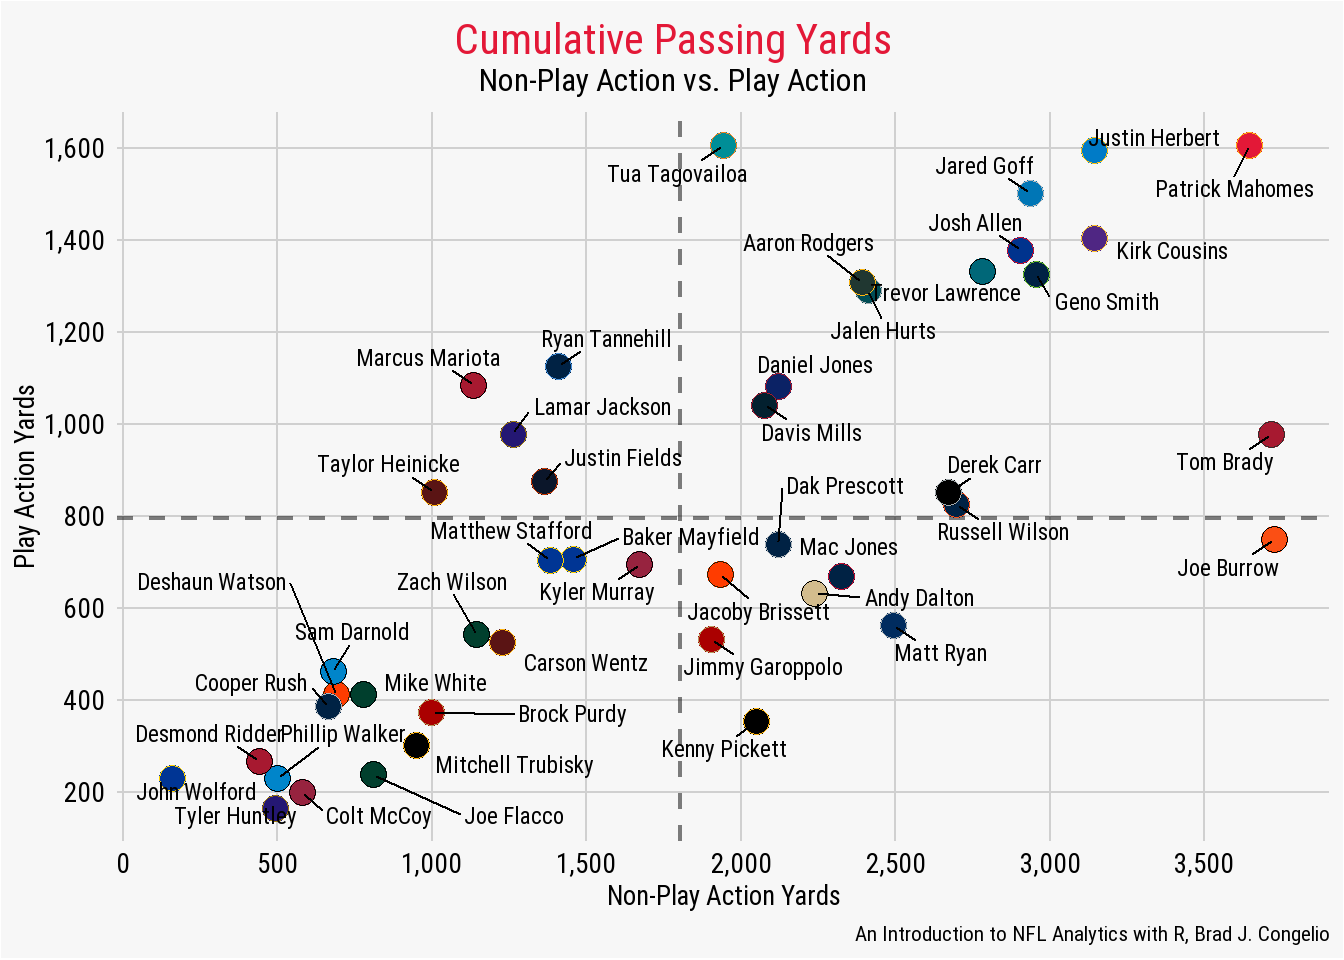
\includegraphics{04-nfl-analytics-visualization_files/figure-pdf/adding-theme-elements-to-plot-1.pdf}

}

\end{figure}

There is a lot going on now in our \texttt{theme()} argument.
Importantly, you may notice that we used \texttt{element\_blank()} to
remove the axis tick marks, but then switched to using
\texttt{element\_text()} for the reminder of the edits with our
\texttt{theme()}. Both are one of four theme elements that can be
modified in the above fashion.

\begin{tcolorbox}[enhanced jigsaw, left=2mm, toprule=.15mm, opacitybacktitle=0.6, leftrule=.75mm, bottomrule=.15mm, colbacktitle=quarto-callout-tip-color!10!white, breakable, colback=white, bottomtitle=1mm, toptitle=1mm, title=\textcolor{quarto-callout-tip-color}{\faLightbulb}\hspace{0.5em}{Tip}, coltitle=black, titlerule=0mm, arc=.35mm, opacityback=0, colframe=quarto-callout-tip-color-frame, rightrule=.15mm]

\textbf{The Four Theme Elements You Can Edit}

When working on editing your plot to your liking, you can make changes
to one of four theme elements:

\begin{enumerate}
\def\labelenumi{\arabic{enumi}.}
\tightlist
\item
  \texttt{element\_blank()} - this used to entirely remove an element
  from the plot like we did with \texttt{axis.ticks}.
\item
  \texttt{element\_rect()} - this is used to make changes to the borders
  and backgrounds of a plot.
\item
  \texttt{element\_lines()} - this is used to make changes to any
  element in the plot that is a line.
\item
  \texttt{element\_text()} - this is used to make change to any element
  in the plot that is text.
\end{enumerate}

\end{tcolorbox}

We first made changes to the text of the title associated with the x-
and y-axis and made edits to the text of the numeric values for each
yardage distance. This process is started by using \texttt{axis.title}
and \texttt{axis.text} in conjunction with \texttt{element\_text()},
since that is the specific element type we are wishing to edit. Within
our \texttt{element\_text()}, we provided the numerous argument on how
we wished to edit the text of both by providing the \texttt{family} (or
the font), the \texttt{face}, the \texttt{size}, and the \texttt{color}.

After, we got a little fancy in our edits to our plots title and
subtitle. I knew that I wanted to center both directly in the middle of
the plot. Rather than figuring out the specific horizontal adjustment
needed, I used the \texttt{plot.title.position()} argument and set it to
\texttt{"plot"}, which used the entire width of our plot as the
reference point for where to center the plot title and subtitle.

To take advantage of this, we followed by using the
\texttt{plot.title()} argument to set the title's horizontal adjustment
to 0.5 (\texttt{hjust\ =\ 0.5}). As you may guess, the inclusion of 0.5
instructs the output to center the title (and the subtitle in the
ensuing edit) directly over the middle of the plot (as calculated
through our prior use of \texttt{plot.title.position()}.

Our next significant changes occurred by changing the aesthetics of the
plot's grid lines, background, and border. Because we are working with
either line or background elements, we switch from
\texttt{element\_text()} and begin to use either
\texttt{element\_line()} or \texttt{element\_rect()} (as well as again
using \texttt{element\_blank()} to completely remove the panel's minor
grid lines).

\begin{tcolorbox}[enhanced jigsaw, left=2mm, toprule=.15mm, opacitybacktitle=0.6, leftrule=.75mm, bottomrule=.15mm, colbacktitle=quarto-callout-tip-color!10!white, breakable, colback=white, bottomtitle=1mm, toptitle=1mm, title=\textcolor{quarto-callout-tip-color}{\faLightbulb}\hspace{0.5em}{Tip}, coltitle=black, titlerule=0mm, arc=.35mm, opacityback=0, colframe=quarto-callout-tip-color-frame, rightrule=.15mm]

\textbf{In a plot, which are the minor grid lines and which are the
major?}

In a \texttt{ggplot2} plot, \textbf{minor grid lines} are those lines
that hit either the x- or y-axis between the continuous or discrete
values. Conversely, \textbf{major grid lines} are the lines that hit the
axis at the same spot as the data values.

In the case of the current plot, our major grid lines are those that hit
the x-axis at 500, 1,000, 1,500, and so on and hit the y-axis at 400,
600, 800, etc. The minor grid lines met the axis between the major grid
lines.

\end{tcolorbox}

After removing the panel's minor grid lines (again, a personal
preference of mine), we also change the color of the panel's major grid
lines, then change the color of the plot's background (both using
\texttt{element\_rect()}). The end result is a aesthetically pleasing
data visualization.

\hypertarget{creating-your-own-ggplot2-theme}{%
\section{\texorpdfstring{Creating Your Own \texttt{ggplot2}
Theme}{Creating Your Own ggplot2 Theme}}\label{creating-your-own-ggplot2-theme}}

As mentioned, I have a distinctive ``brand and look'' for the data
visualizations I create that make use of the same design elements and
choices. Rather than copy and paste those into each and every
\texttt{ggplot} piece of code I write, I've opted to consolidate all the
\texttt{theme()} element changes into my own
\texttt{nfl\_analytics\_theme()} function. In much the same way, I've
created a ``quick and easy'' theme for use in this book. To get started,
running the following chunk of code will create a function titled
\texttt{nfl\_analytics\_theme} and place it into your RStudio
environment.

\begin{Shaded}
\begin{Highlighting}[]
\NormalTok{nfl\_analytics\_theme }\OtherTok{\textless{}{-}} \ControlFlowTok{function}\NormalTok{(..., }\AttributeTok{base\_size =} \DecValTok{12}\NormalTok{) \{}
  
    \FunctionTok{theme}\NormalTok{(}
      \AttributeTok{text =} \FunctionTok{element\_text}\NormalTok{(}\AttributeTok{family =} \StringTok{"Roboto"}\NormalTok{, }\AttributeTok{size =}\NormalTok{ base\_size),}
      \AttributeTok{axis.ticks =} \FunctionTok{element\_blank}\NormalTok{(),}
      \AttributeTok{axis.title =} \FunctionTok{element\_text}\NormalTok{(}\AttributeTok{color =} \StringTok{"black"}\NormalTok{,}
                                \AttributeTok{face =} \StringTok{"bold"}\NormalTok{),}
      \AttributeTok{axis.text =} \FunctionTok{element\_text}\NormalTok{(}\AttributeTok{color =} \StringTok{"black"}\NormalTok{,}
                               \AttributeTok{face =} \StringTok{"bold"}\NormalTok{),}
      \AttributeTok{plot.title.position =} \StringTok{"plot"}\NormalTok{,}
      \AttributeTok{plot.title =} \FunctionTok{element\_text}\NormalTok{(}\AttributeTok{size =} \DecValTok{16}\NormalTok{,}
                                \AttributeTok{face =} \StringTok{"bold"}\NormalTok{,}
                                \AttributeTok{color =} \StringTok{"black"}\NormalTok{,}
                                \AttributeTok{vjust =}\NormalTok{ .}\DecValTok{02}\NormalTok{,}
                                \AttributeTok{hjust =} \FloatTok{0.5}\NormalTok{),}
      \AttributeTok{plot.subtitle =} \FunctionTok{element\_text}\NormalTok{(}\AttributeTok{color =} \StringTok{"black"}\NormalTok{,}
                                   \AttributeTok{hjust =} \FloatTok{0.5}\NormalTok{),}
      \AttributeTok{plot.caption =} \FunctionTok{element\_text}\NormalTok{(}\AttributeTok{size =} \DecValTok{8}\NormalTok{,}
                                  \AttributeTok{face =} \StringTok{"italic"}\NormalTok{,}
                                  \AttributeTok{color =} \StringTok{"black"}\NormalTok{),}
      \AttributeTok{panel.grid.minor =} \FunctionTok{element\_blank}\NormalTok{(),}
      \AttributeTok{panel.grid.major =}  \FunctionTok{element\_line}\NormalTok{(}\AttributeTok{color =} \StringTok{"\#d0d0d0"}\NormalTok{),}
      \AttributeTok{panel.background =} \FunctionTok{element\_rect}\NormalTok{(}\AttributeTok{fill =} \StringTok{"\#f7f7f7"}\NormalTok{),}
      \AttributeTok{plot.background =} \FunctionTok{element\_rect}\NormalTok{(}\AttributeTok{fill =} \StringTok{"\#f7f7f7"}\NormalTok{),}
      \AttributeTok{panel.border =} \FunctionTok{element\_blank}\NormalTok{())}
\NormalTok{\}}
\end{Highlighting}
\end{Shaded}

You may notice that the elements in the above theme creation are quite
similar to the ones we passed into our previous plot. And that is true,
and the results will be nearly 99.9\% identical. After wrapping our
\texttt{theme()} inside a function, indicated by the opening and closing
curly brackets \texttt{\{\ \}}, we can provide our desired theme element
appearances as we would within a regular \texttt{ggplot2} code block.

However, in the above theme function, we have streamlined the basis a
bit by indicating a \texttt{base\_size} of all the text, when means all
text output will be in size 12 font unless specifically indicated in the
element (for example, we have the \texttt{plot.title} set to have a
\texttt{size} of 16). As well, the same process was done for font
(Roboto) so there was not a need to type it repeatedly into every
element.

Based on the above example, you are free to create as detailed a theme
function as you desire. The beauty of creating your own theme like above
is you will no longer need to edit each portion of the every plot
element. Rather, you can simply call in your theme after you run it and
it resides in under the ``Functions'' in your RStudio environment.

\begin{Shaded}
\begin{Highlighting}[]
\FunctionTok{ggplot}\NormalTok{(}\AttributeTok{data =}\NormalTok{ play\_action\_data, }\FunctionTok{aes}\NormalTok{(}\AttributeTok{x =}\NormalTok{ yds, }\AttributeTok{y =}\NormalTok{ pa\_yds)) }\SpecialCharTok{+}
  \FunctionTok{geom\_mean\_lines}\NormalTok{(}\FunctionTok{aes}\NormalTok{(}\AttributeTok{v\_var =}\NormalTok{ yds, }\AttributeTok{h\_var =}\NormalTok{ pa\_yds), }
                  \AttributeTok{size =} \FloatTok{0.8}\NormalTok{,}
                  \AttributeTok{color =} \StringTok{"black"}\NormalTok{, }
                  \AttributeTok{linetype =} \StringTok{"dashed"}\NormalTok{,}
                  \AttributeTok{alpha =} \FloatTok{0.5}\NormalTok{) }\SpecialCharTok{+}
  \FunctionTok{geom\_point}\NormalTok{(}\AttributeTok{shape =} \DecValTok{21}\NormalTok{,}
             \AttributeTok{fill =}\NormalTok{ play\_action\_data}\SpecialCharTok{$}\NormalTok{team\_color,}
             \AttributeTok{color =}\NormalTok{ play\_action\_data}\SpecialCharTok{$}\NormalTok{team\_color2,}
             \AttributeTok{size =} \FloatTok{4.5}\NormalTok{) }\SpecialCharTok{+}
  \FunctionTok{geom\_text\_repel}\NormalTok{(}\FunctionTok{aes}\NormalTok{(}\AttributeTok{label =}\NormalTok{ player),}
                  \AttributeTok{box.padding =} \FloatTok{0.45}\NormalTok{,}
                  \AttributeTok{size =} \DecValTok{3}\NormalTok{,}
                  \AttributeTok{family =} \StringTok{"Roboto"}\NormalTok{,}
                  \AttributeTok{fontface =} \StringTok{"bold"}\NormalTok{) }\SpecialCharTok{+}
  \FunctionTok{scale\_x\_continuous}\NormalTok{(}\AttributeTok{breaks =}\NormalTok{ scales}\SpecialCharTok{::}\FunctionTok{pretty\_breaks}\NormalTok{(}\AttributeTok{n =} \DecValTok{6}\NormalTok{),}
                     \AttributeTok{labels =}\NormalTok{ scales}\SpecialCharTok{::}\FunctionTok{label\_comma}\NormalTok{()) }\SpecialCharTok{+}
  \FunctionTok{scale\_y\_continuous}\NormalTok{(}\AttributeTok{breaks =}\NormalTok{ scales}\SpecialCharTok{::}\FunctionTok{pretty\_breaks}\NormalTok{(}\AttributeTok{n =} \DecValTok{6}\NormalTok{),}
                     \AttributeTok{labels =}\NormalTok{ scales}\SpecialCharTok{::}\FunctionTok{label\_comma}\NormalTok{()) }\SpecialCharTok{+}
  \FunctionTok{labs}\NormalTok{(}\AttributeTok{x =} \StringTok{"Non{-}Play Action Yards"}\NormalTok{,}
       \AttributeTok{y =} \StringTok{"Play Action Yards"}\NormalTok{,}
       \AttributeTok{title =} \StringTok{"**Cumulative Passing Yards**"}\NormalTok{,}
       \AttributeTok{subtitle =} \StringTok{"*Non{-}Play Action vs. Play Action*"}\NormalTok{,}
       \AttributeTok{caption =} \StringTok{"*An Introduction to NFL Analytics with R*\textless{}br\textgreater{}**Brad J. Congelio**"}\NormalTok{) }\SpecialCharTok{+}
  \FunctionTok{nfl\_analytics\_theme}\NormalTok{()}
\end{Highlighting}
\end{Shaded}

\begin{verbatim}
Warning: ggrepel: 21 unlabeled data points (too many overlaps). Consider
increasing max.overlaps
\end{verbatim}

\begin{figure}[H]

{\centering 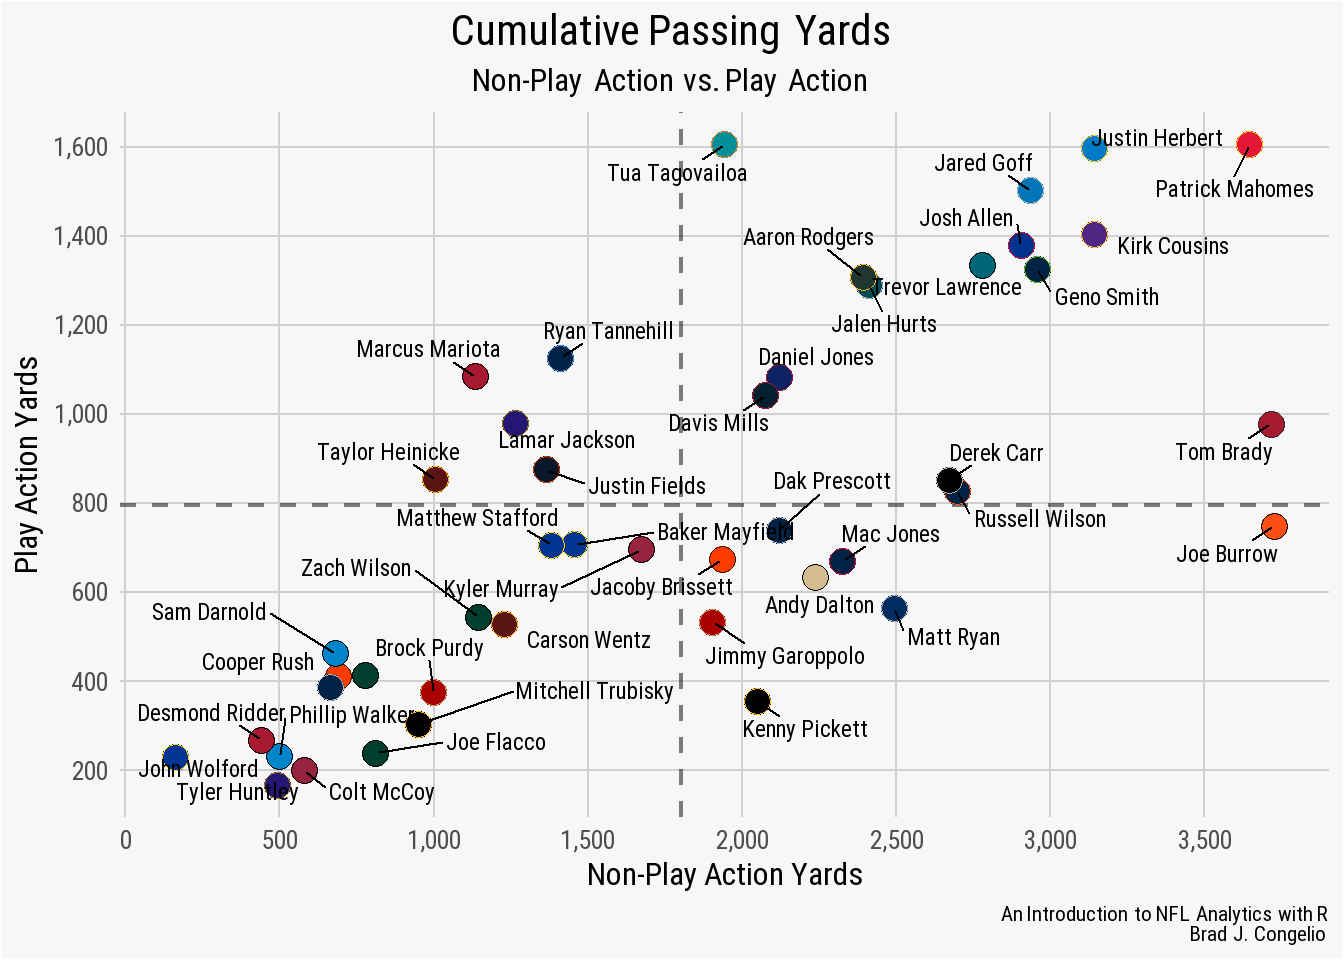
\includegraphics{04-nfl-analytics-visualization_files/figure-pdf/showcasing-use-of-theme-1.pdf}

}

\end{figure}

As you can see, we just consolidated 28 lines of code into a
\textbf{single line of code by wrapping all our theme elements into an
easy to construct function.}

Unfortunately, you will notice that the resulting plot does not output
with the title (``Cumulative Passing Yards'') in Kansas City red like in
our original. This is because, in our \texttt{nfl\_analytics\_theme()}
function, the \texttt{color} for \texttt{axis.title()} is set to
\texttt{"black"}. Thankfully, we can make this small edit within our
\texttt{ggplot} code to switch the title back to Kansas City red,
highlighting the idea that - despite the theme being built into a
function - we still have the ability to make necessary edits on the fly
without including all 28 lines of code. With the
\texttt{nfl\_analytics\_theme()} active, we can still add additional
\texttt{theme} elements as needed to make modifications, as seen below.

\begin{Shaded}
\begin{Highlighting}[]
\FunctionTok{ggplot}\NormalTok{(}\AttributeTok{data =}\NormalTok{ play\_action\_data, }\FunctionTok{aes}\NormalTok{(}\AttributeTok{x =}\NormalTok{ yds, }\AttributeTok{y =}\NormalTok{ pa\_yds)) }\SpecialCharTok{+}
  \FunctionTok{geom\_mean\_lines}\NormalTok{(}\FunctionTok{aes}\NormalTok{(}\AttributeTok{v\_var =}\NormalTok{ yds, }\AttributeTok{h\_var =}\NormalTok{ pa\_yds), }
                  \AttributeTok{size =} \FloatTok{0.8}\NormalTok{,}
                  \AttributeTok{color =} \StringTok{"black"}\NormalTok{, }
                  \AttributeTok{linetype =} \StringTok{"dashed"}\NormalTok{,}
                  \AttributeTok{alpha =} \FloatTok{0.5}\NormalTok{) }\SpecialCharTok{+}
  \FunctionTok{geom\_point}\NormalTok{(}\AttributeTok{shape =} \DecValTok{21}\NormalTok{,}
             \AttributeTok{fill =}\NormalTok{ play\_action\_data}\SpecialCharTok{$}\NormalTok{team\_color,}
             \AttributeTok{color =}\NormalTok{ play\_action\_data}\SpecialCharTok{$}\NormalTok{team\_color2,}
             \AttributeTok{size =} \FloatTok{4.5}\NormalTok{) }\SpecialCharTok{+}
  \FunctionTok{geom\_text\_repel}\NormalTok{(}\FunctionTok{aes}\NormalTok{(}\AttributeTok{label =}\NormalTok{ player),}
                  \AttributeTok{box.padding =} \FloatTok{0.45}\NormalTok{,}
                  \AttributeTok{size =} \DecValTok{3}\NormalTok{,}
                  \AttributeTok{family =} \StringTok{"Roboto"}\NormalTok{,}
                  \AttributeTok{fontface =} \StringTok{"bold"}\NormalTok{) }\SpecialCharTok{+}
  \FunctionTok{scale\_x\_continuous}\NormalTok{(}\AttributeTok{breaks =}\NormalTok{ scales}\SpecialCharTok{::}\FunctionTok{pretty\_breaks}\NormalTok{(}\AttributeTok{n =} \DecValTok{6}\NormalTok{),}
                     \AttributeTok{labels =}\NormalTok{ scales}\SpecialCharTok{::}\FunctionTok{label\_comma}\NormalTok{()) }\SpecialCharTok{+}
  \FunctionTok{scale\_y\_continuous}\NormalTok{(}\AttributeTok{breaks =}\NormalTok{ scales}\SpecialCharTok{::}\FunctionTok{pretty\_breaks}\NormalTok{(}\AttributeTok{n =} \DecValTok{6}\NormalTok{),}
                     \AttributeTok{labels =}\NormalTok{ scales}\SpecialCharTok{::}\FunctionTok{label\_comma}\NormalTok{()) }\SpecialCharTok{+}
  \FunctionTok{labs}\NormalTok{(}\AttributeTok{x =} \StringTok{"Non{-}Play Action Yards"}\NormalTok{,}
       \AttributeTok{y =} \StringTok{"Play Action Yards"}\NormalTok{,}
       \AttributeTok{title =} \StringTok{"**Cumulative Passing Yards**"}\NormalTok{,}
       \AttributeTok{subtitle =} \StringTok{"*Non{-}Play Action vs. Play Action*"}\NormalTok{,}
       \AttributeTok{caption =} \StringTok{"*An Introduction to NFL Analytics with R*\textless{}br\textgreater{}**Brad J. Congelio**"}\NormalTok{) }\SpecialCharTok{+}
  \FunctionTok{nfl\_analytics\_theme}\NormalTok{() }\SpecialCharTok{+}
  \FunctionTok{theme}\NormalTok{(}\AttributeTok{plot.title =} \FunctionTok{element\_markdown}\NormalTok{(}\AttributeTok{color =} \StringTok{"\#E31837"}\NormalTok{))}
\end{Highlighting}
\end{Shaded}

\begin{verbatim}
Warning: ggrepel: 21 unlabeled data points (too many overlaps). Consider
increasing max.overlaps
\end{verbatim}

\begin{figure}[H]

{\centering 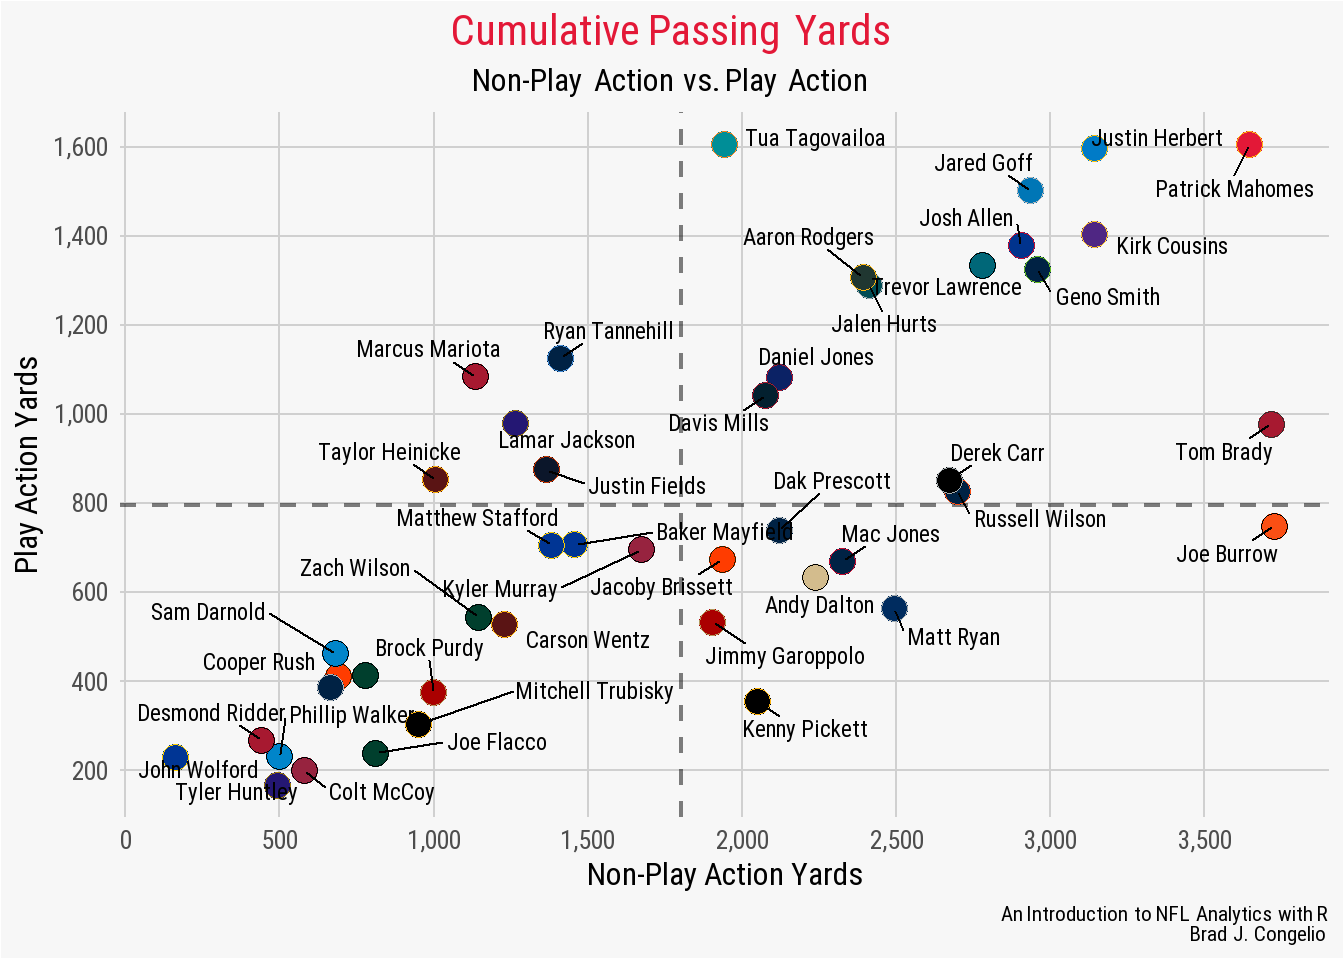
\includegraphics{04-nfl-analytics-visualization_files/figure-pdf/theme-code-with-modification-1.pdf}

}

\end{figure}

\hypertarget{using-team-logos-in-plots}{%
\section{Using Team Logos in Plots}\label{using-team-logos-in-plots}}

To explore the process of placing team logos into a plot, let's stick
with our previous example of working with play action passing data but
explore it at the team level rather than individual quarterbacks. To
gather the data, we can use \texttt{vroom} to read it in from the book's
GitHub.

\begin{Shaded}
\begin{Highlighting}[]
\NormalTok{team\_playaction }\OtherTok{\textless{}{-}}
  \FunctionTok{vroom}\NormalTok{(}\StringTok{"https://raw.githubusercontent.com/bcongelio/nfl{-}analytics{-}with{-}r{-}book/origin/example\_data/csv/team\_playaction.csv"}\NormalTok{)}
\end{Highlighting}
\end{Shaded}

The resulting \texttt{team\_playaction} data contains nearly identical
information to the previous QB-level data. However, there is a slight
change in how Sports Info Solutions charts passing yards on the team
level. You will notice a column for both \texttt{net\_yds} and
\texttt{gross\_yds}. When charting passing attempts in football, a
player's individual passing yards are aggregated under \textbf{gross
yards} with all lost yardage resulting from a sack being included. On
the other hand, team passing yards are always presented in \textbf{net
yards} and any lost yardage from sacks are not included. Case in point,
the \texttt{gross\_yds} number in our \texttt{team\_playaction} data is
greater than the \texttt{net\_yds} for all 32 NFL teams. In any case, we
will build our data visualization using \texttt{net\_yds}.

In order to include team logos in the plot, we must first merge in team
logo information (again with the understanding that we could use
\texttt{nflplotR} if team abbreviations were included in the data). We
can collect the team logo information using the \texttt{load\_teams()}
function within \texttt{nflreadR}. There are three different variations
of each team's logo available in the resulting data: (1.) the logo from
ESPN, (2.) the logo from Wikipedia, (3.) a pre-edited version of the
logo that is cropped into a square.

\begin{tcolorbox}[enhanced jigsaw, left=2mm, toprule=.15mm, opacitybacktitle=0.6, leftrule=.75mm, bottomrule=.15mm, colbacktitle=quarto-callout-note-color!10!white, breakable, colback=white, bottomtitle=1mm, toptitle=1mm, title=\textcolor{quarto-callout-note-color}{\faInfo}\hspace{0.5em}{Note}, coltitle=black, titlerule=0mm, arc=.35mm, opacityback=0, colframe=quarto-callout-note-color-frame, rightrule=.15mm]

\textbf{There are slight differences in disk space, pixels, and utility
in the provided ESPN, Wikipedia, and squared versions of the logos.}

The Wikipedia versions are, generally, smaller in size. The Arizona
Cardinals logo, for example, is just 9.11 KB in size from Wikipedia
while the ESPN version of the logo is 20.6 KB. This difference is disk
size is the result of each images dimensions and pixels. The ESPN
version, with the larger disk size, is also a higher quality image that
is scaled in 500x500 dimensions (and 500 pixels). The Wikipedia version
is scaled in 179x161 dimensions at 179 pixels and 161 pixels,
respectively. The squared version of the logo is a 200x200 image at 200
pixels with a background matching the team's primary color.

What does this mean? The ESPN version of the logo is better for those
applications where the logo will be large and you do not want any loss
of quality. The Wikipedia version, conversely, is better suited for
applications like our: for use in a small-scale data visualization. We
do not plan on ``blowing up'' the image, thus losing quality and the
smaller disk space size of the images allows for a slightly quicker
rendering time when we use the \texttt{ggimage} package. While sparingly
used, the squared version of the logo can be used in certain data
visualization applications that requires the team logo to quickly and
easily ``merge'' into the background of the plot (more on this later in
this chapter, though).

\end{tcolorbox}

Because of the above explanation, we can collect just the team nicknames
and the Wikipedia version of the logo to merge into our existing
\texttt{team\_playaction} data.

\begin{Shaded}
\begin{Highlighting}[]
\NormalTok{teams }\OtherTok{\textless{}{-}}\NormalTok{ nflreadr}\SpecialCharTok{::}\FunctionTok{load\_teams}\NormalTok{(}\AttributeTok{current =} \ConstantTok{TRUE}\NormalTok{) }\SpecialCharTok{\%\textgreater{}\%}
  \FunctionTok{select}\NormalTok{(team\_nick, team\_logo\_wikipedia)}

\NormalTok{team\_playaction }\OtherTok{\textless{}{-}}\NormalTok{ team\_playaction }\SpecialCharTok{\%\textgreater{}\%}
  \FunctionTok{left\_join}\NormalTok{(teams, }\AttributeTok{by =} \FunctionTok{c}\NormalTok{(}\StringTok{"team"} \OtherTok{=} \StringTok{"team\_nick"}\NormalTok{))}

\NormalTok{team\_playaction}
\end{Highlighting}
\end{Shaded}

With the data now containing the correct information, we can build a
basic version of our data visualization using the same
\texttt{geom\_point} as above, and continue to configure the information
on both the x- and y-axis, to verify that everything is working
correctly before switching out \texttt{geom\_point} for
\texttt{geom\_image} in order to bring the team logos into the plot.

\begin{Shaded}
\begin{Highlighting}[]
\FunctionTok{ggplot}\NormalTok{(}\AttributeTok{data =}\NormalTok{ team\_playaction, }\FunctionTok{aes}\NormalTok{(}\AttributeTok{x =}\NormalTok{ net\_yds, }\AttributeTok{y =}\NormalTok{ pa\_net\_yds)) }\SpecialCharTok{+}
  \FunctionTok{geom\_hline}\NormalTok{(}\AttributeTok{yintercept =} \FunctionTok{mean}\NormalTok{(team\_playaction}\SpecialCharTok{$}\NormalTok{pa\_net\_yds), }
             \AttributeTok{linewidth =} \FloatTok{0.8}\NormalTok{, }
             \AttributeTok{color =} \StringTok{"black"}\NormalTok{, }
             \AttributeTok{linetype =} \StringTok{"dashed"}\NormalTok{) }\SpecialCharTok{+}
  \FunctionTok{geom\_vline}\NormalTok{(}\AttributeTok{xintercept =} \FunctionTok{mean}\NormalTok{(team\_playaction}\SpecialCharTok{$}\NormalTok{net\_yds), }
             \AttributeTok{linewidth =} \FloatTok{0.8}\NormalTok{, }
             \AttributeTok{color =} \StringTok{"black"}\NormalTok{, }
             \AttributeTok{linetype =} \StringTok{"dashed"}\NormalTok{) }\SpecialCharTok{+}
  \FunctionTok{geom\_point}\NormalTok{() }\SpecialCharTok{+}
  \FunctionTok{scale\_x\_continuous}\NormalTok{(}\AttributeTok{breaks =}\NormalTok{ scales}\SpecialCharTok{::}\FunctionTok{pretty\_breaks}\NormalTok{(}\AttributeTok{n =} \DecValTok{6}\NormalTok{),}
                     \AttributeTok{labels =}\NormalTok{ scales}\SpecialCharTok{::}\FunctionTok{label\_comma}\NormalTok{()) }\SpecialCharTok{+}
  \FunctionTok{scale\_y\_continuous}\NormalTok{(}\AttributeTok{breaks =}\NormalTok{ scales}\SpecialCharTok{::}\FunctionTok{pretty\_breaks}\NormalTok{(}\AttributeTok{n =} \DecValTok{6}\NormalTok{),}
                     \AttributeTok{labels =}\NormalTok{ scales}\SpecialCharTok{::}\FunctionTok{label\_comma}\NormalTok{()) }\SpecialCharTok{+}
  \FunctionTok{labs}\NormalTok{(}\AttributeTok{title =} \StringTok{"**Net Passing Yards Without Play Action vs. With Play Action**"}\NormalTok{,}
       \AttributeTok{subtitle =} \StringTok{"*2022 NFL Regular Season*"}\NormalTok{,}
       \AttributeTok{caption =} \StringTok{"*An Introduction to NFL Analytics with R*\textless{}br\textgreater{}**Brad J. Congelio**"}\NormalTok{,}
       \AttributeTok{x =} \StringTok{"Net Yards Without Play Action"}\NormalTok{,}
       \AttributeTok{y =} \StringTok{"Net Yards With Play Action"}\NormalTok{) }\SpecialCharTok{+}
  \FunctionTok{nfl\_analytics\_theme}\NormalTok{()}
\end{Highlighting}
\end{Shaded}

\begin{figure}[H]

{\centering 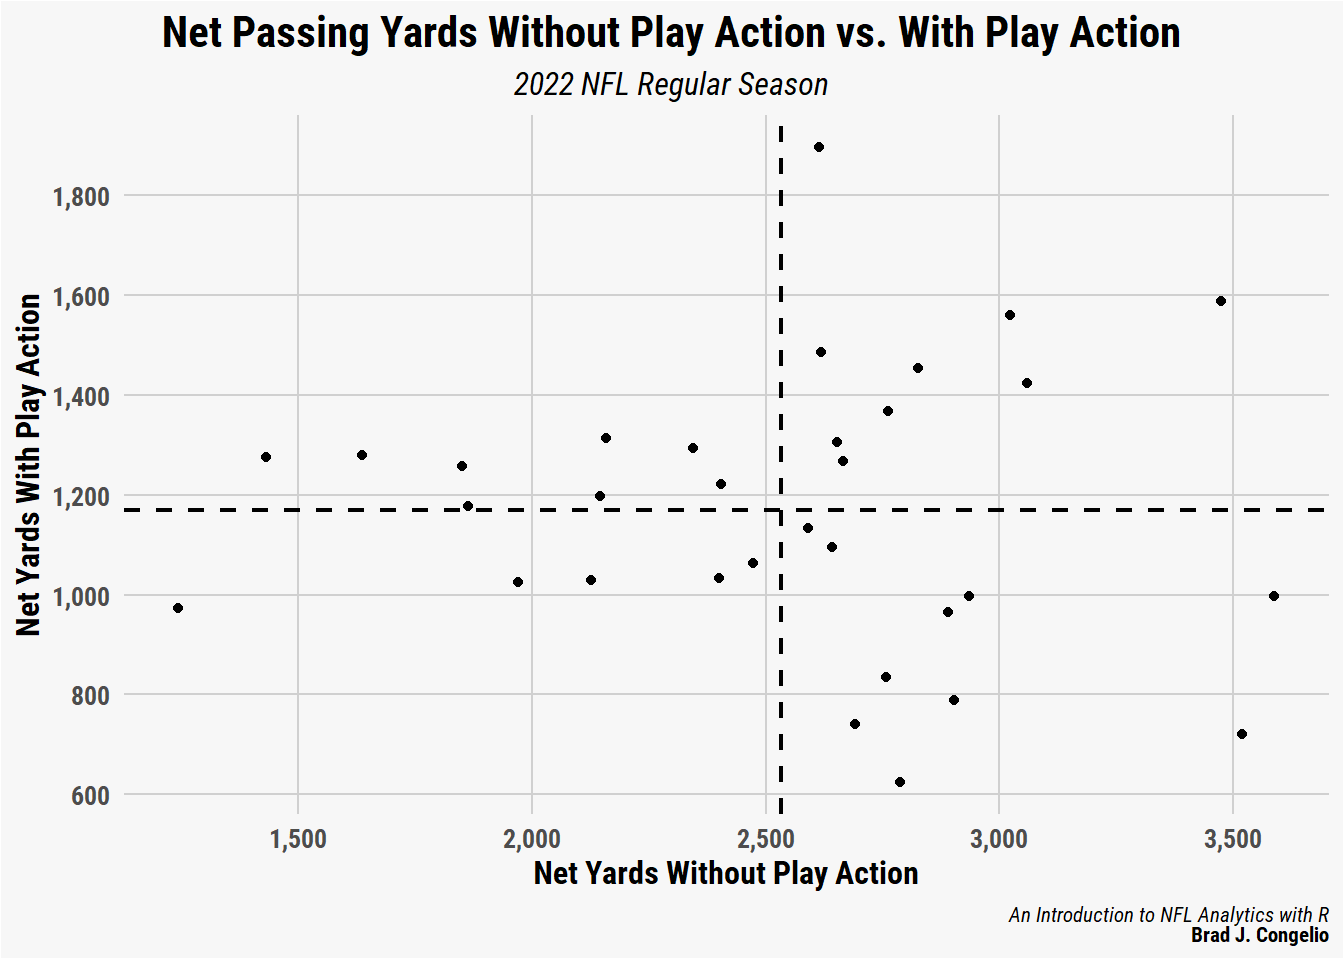
\includegraphics{04-nfl-analytics-visualization_files/figure-pdf/building-initial-team-pa-1.pdf}

}

\end{figure}

The resulting plot, constructed in nearly an identical manner to our
above example, looks correct and we are ready to swap out
\texttt{geom\_point} for team logos.

\begin{tcolorbox}[enhanced jigsaw, left=2mm, toprule=.15mm, opacitybacktitle=0.6, leftrule=.75mm, bottomrule=.15mm, colbacktitle=quarto-callout-important-color!10!white, breakable, colback=white, bottomtitle=1mm, toptitle=1mm, title=\textcolor{quarto-callout-important-color}{\faExclamation}\hspace{0.5em}{Important}, coltitle=black, titlerule=0mm, arc=.35mm, opacityback=0, colframe=quarto-callout-important-color-frame, rightrule=.15mm]

Before proceeding with this next step, be sure that you have the
\texttt{ggimage} package installed and loaded.

\end{tcolorbox}

\begin{Shaded}
\begin{Highlighting}[]
\FunctionTok{ggplot}\NormalTok{(}\AttributeTok{data =}\NormalTok{ team\_playaction, }\FunctionTok{aes}\NormalTok{(}\AttributeTok{x =}\NormalTok{ net\_yds, }\AttributeTok{y =}\NormalTok{ pa\_net\_yds)) }\SpecialCharTok{+}
  \FunctionTok{geom\_hline}\NormalTok{(}\AttributeTok{yintercept =} \FunctionTok{mean}\NormalTok{(team\_playaction}\SpecialCharTok{$}\NormalTok{pa\_net\_yds), }
             \AttributeTok{linewidth =} \FloatTok{0.8}\NormalTok{, }
             \AttributeTok{color =} \StringTok{"black"}\NormalTok{, }
             \AttributeTok{linetype =} \StringTok{"dashed"}\NormalTok{) }\SpecialCharTok{+}
  \FunctionTok{geom\_vline}\NormalTok{(}\AttributeTok{xintercept =} \FunctionTok{mean}\NormalTok{(team\_playaction}\SpecialCharTok{$}\NormalTok{net\_yds), }
             \AttributeTok{linewidth =} \FloatTok{0.8}\NormalTok{, }
             \AttributeTok{color =} \StringTok{"black"}\NormalTok{, }
             \AttributeTok{linetype =} \StringTok{"dashed"}\NormalTok{) }\SpecialCharTok{+}
  \FunctionTok{geom\_image}\NormalTok{(}\FunctionTok{aes}\NormalTok{(}\AttributeTok{image =}\NormalTok{ team\_logo\_wikipedia)) }\SpecialCharTok{+}
  \FunctionTok{scale\_x\_continuous}\NormalTok{(}\AttributeTok{breaks =}\NormalTok{ scales}\SpecialCharTok{::}\FunctionTok{pretty\_breaks}\NormalTok{(}\AttributeTok{n =} \DecValTok{6}\NormalTok{),}
                     \AttributeTok{labels =}\NormalTok{ scales}\SpecialCharTok{::}\FunctionTok{label\_comma}\NormalTok{()) }\SpecialCharTok{+}
  \FunctionTok{scale\_y\_continuous}\NormalTok{(}\AttributeTok{breaks =}\NormalTok{ scales}\SpecialCharTok{::}\FunctionTok{pretty\_breaks}\NormalTok{(}\AttributeTok{n =} \DecValTok{6}\NormalTok{),}
                     \AttributeTok{labels =}\NormalTok{ scales}\SpecialCharTok{::}\FunctionTok{label\_comma}\NormalTok{()) }\SpecialCharTok{+}
  \FunctionTok{labs}\NormalTok{(}\AttributeTok{title =} \StringTok{"**Net Passing Yards Without Play Action vs. With Play Action**"}\NormalTok{,}
       \AttributeTok{subtitle =} \StringTok{"*2022 NFL Regular Season*"}\NormalTok{,}
       \AttributeTok{caption =} \StringTok{"*An Introduction to NFL Analytics with R*\textless{}br\textgreater{}**Brad J. Congelio**"}\NormalTok{,}
       \AttributeTok{x =} \StringTok{"Net Yards Without Play Action"}\NormalTok{,}
       \AttributeTok{y =} \StringTok{"Net Yards With Play Action"}\NormalTok{) }\SpecialCharTok{+}
  \FunctionTok{nfl\_analytics\_theme}\NormalTok{()}
\end{Highlighting}
\end{Shaded}

\begin{figure}[H]

{\centering 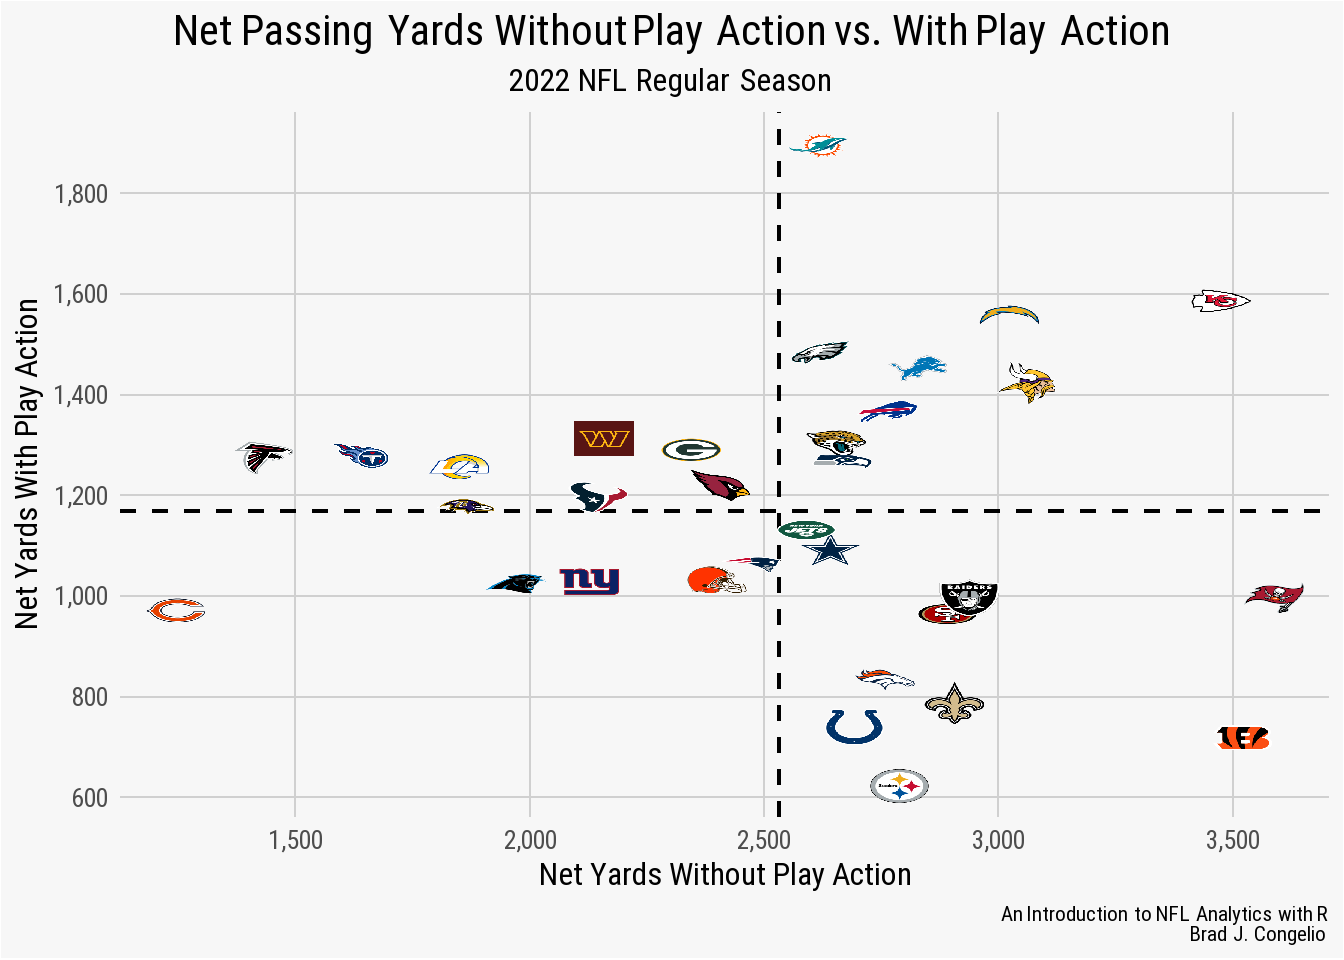
\includegraphics{04-nfl-analytics-visualization_files/figure-pdf/adding-logos-without-aspect-1.pdf}

}

\end{figure}

By using the \texttt{geom\_image} function, we are able to wrap the
\texttt{image} argument within an aesthetics call (that is,
\texttt{aes()}) and then stipulate that the
\texttt{team\_logo\_wikipedia} variable is to serve as the image
associated with each data point.

But, wait: \textbf{the image looks horrible, right?} Indeed, the logos
are pixelated, are skewed in shape, and are just generally unpleasant to
look at.

That is because we failed to provide an aspect ratio for the team logos.
In this case, we need to add \texttt{asp\ =\ 16/9}.

\begin{tcolorbox}[enhanced jigsaw, left=2mm, toprule=.15mm, opacitybacktitle=0.6, leftrule=.75mm, bottomrule=.15mm, colbacktitle=quarto-callout-note-color!10!white, breakable, colback=white, bottomtitle=1mm, toptitle=1mm, title=\textcolor{quarto-callout-note-color}{\faInfo}\hspace{0.5em}{Note}, coltitle=black, titlerule=0mm, arc=.35mm, opacityback=0, colframe=quarto-callout-note-color-frame, rightrule=.15mm]

Why are we including a specific aspect ratio of 16/9 for each team logo?
Good question.

An aspect ratio of 16/9 refers to the proportional relationship between
the width and height of a rectangular display or image. In this case,
the width of the image is 16 units, and the height is 9 units.
Importantly, this aspect ratio is commonly used for widescreen displays,
including most (if not all) modern televisions, computer monitors, and
smartphones.

As well, the 16/9 aspect ratio is sometimes referred to as 1.78:1, which
means that the width is 1.78 times the height of the image. This aspect
ratio is wider than the traditional 4:3 aspect ratio that was common
used in older television and CRT-based computer monitors.

\end{tcolorbox}

We can make the quick adjustment in our prior code to provide the
correct aspect ratio for each of our team logos:

\begin{Shaded}
\begin{Highlighting}[]
\FunctionTok{ggplot}\NormalTok{(}\AttributeTok{data =}\NormalTok{ team\_playaction, }\FunctionTok{aes}\NormalTok{(}\AttributeTok{x =}\NormalTok{ net\_yds, }\AttributeTok{y =}\NormalTok{ pa\_net\_yds)) }\SpecialCharTok{+}
  \FunctionTok{geom\_hline}\NormalTok{(}\AttributeTok{yintercept =} \FunctionTok{mean}\NormalTok{(team\_playaction}\SpecialCharTok{$}\NormalTok{pa\_net\_yds), }
             \AttributeTok{linewidth =} \FloatTok{0.8}\NormalTok{, }
             \AttributeTok{color =} \StringTok{"black"}\NormalTok{, }
             \AttributeTok{linetype =} \StringTok{"dashed"}\NormalTok{) }\SpecialCharTok{+}
  \FunctionTok{geom\_vline}\NormalTok{(}\AttributeTok{xintercept =} \FunctionTok{mean}\NormalTok{(team\_playaction}\SpecialCharTok{$}\NormalTok{net\_yds), }
             \AttributeTok{linewidth =} \FloatTok{0.8}\NormalTok{, }
             \AttributeTok{color =} \StringTok{"black"}\NormalTok{, }
             \AttributeTok{linetype =} \StringTok{"dashed"}\NormalTok{) }\SpecialCharTok{+}
  \FunctionTok{geom\_image}\NormalTok{(}\FunctionTok{aes}\NormalTok{(}\AttributeTok{image =}\NormalTok{ team\_logo\_wikipedia), }\AttributeTok{asp =} \DecValTok{16}\SpecialCharTok{/}\DecValTok{9}\NormalTok{) }\SpecialCharTok{+}
  \FunctionTok{scale\_x\_continuous}\NormalTok{(}\AttributeTok{breaks =}\NormalTok{ scales}\SpecialCharTok{::}\FunctionTok{pretty\_breaks}\NormalTok{(}\AttributeTok{n =} \DecValTok{6}\NormalTok{),}
                     \AttributeTok{labels =}\NormalTok{ scales}\SpecialCharTok{::}\FunctionTok{label\_comma}\NormalTok{()) }\SpecialCharTok{+}
  \FunctionTok{scale\_y\_continuous}\NormalTok{(}\AttributeTok{breaks =}\NormalTok{ scales}\SpecialCharTok{::}\FunctionTok{pretty\_breaks}\NormalTok{(}\AttributeTok{n =} \DecValTok{6}\NormalTok{),}
                     \AttributeTok{labels =}\NormalTok{ scales}\SpecialCharTok{::}\FunctionTok{label\_comma}\NormalTok{()) }\SpecialCharTok{+}
  \FunctionTok{labs}\NormalTok{(}\AttributeTok{title =} \StringTok{"**Net Passing Yards Without Play Action vs. With Play Action**"}\NormalTok{,}
       \AttributeTok{subtitle =} \StringTok{"*2022 NFL Regular Season*"}\NormalTok{,}
       \AttributeTok{caption =} \StringTok{"*An Introduction to NFL Analytics with R*\textless{}br\textgreater{}**Brad J. Congelio**"}\NormalTok{,}
       \AttributeTok{x =} \StringTok{"Net Yards Without Play Action"}\NormalTok{,}
       \AttributeTok{y =} \StringTok{"Net Yards With Play Action"}\NormalTok{) }\SpecialCharTok{+}
  \FunctionTok{nfl\_analytics\_theme}\NormalTok{()}
\end{Highlighting}
\end{Shaded}

\begin{figure}[H]

{\centering 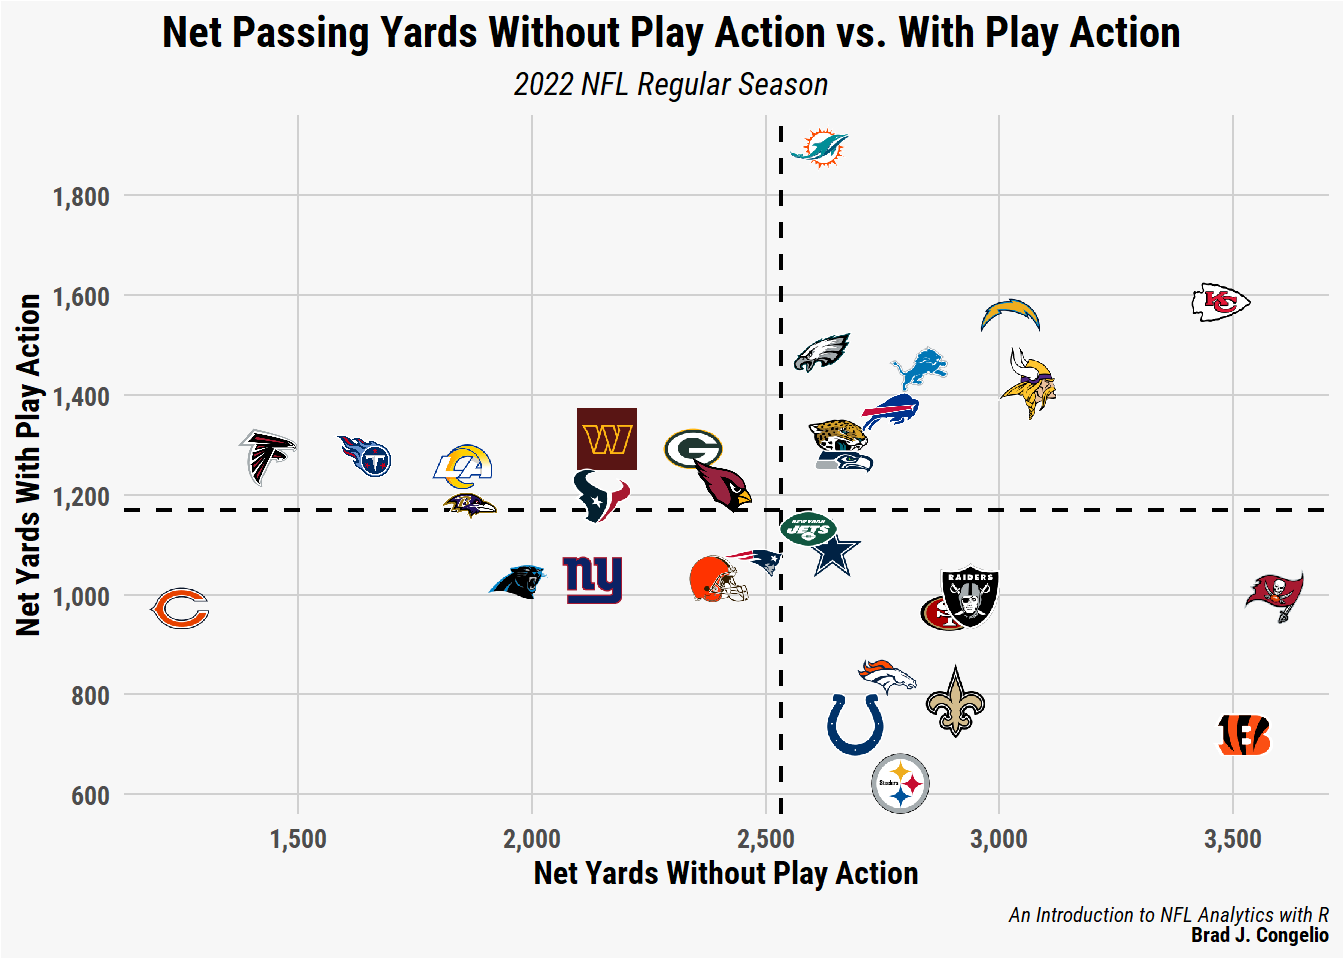
\includegraphics{04-nfl-analytics-visualization_files/figure-pdf/placing-logos-with-correct-asp-1.pdf}

}

\end{figure}

\hypertarget{creating-a-geom_line-plot}{%
\section{\texorpdfstring{Creating a \texttt{geom\_line}
Plot}{Creating a geom\_line Plot}}\label{creating-a-geom_line-plot}}

A \texttt{geom\_line()} plot are useful when you want to display the
trends and/or relationships in data over a continuous variable (such as
seasons). In that context a \texttt{geom\_line()} plot can be used to
explore player statistics over time (such as passing yards and rushing
yards), or to do the same but at the team level, or even comparing one
team against another by including two (or more!) lines on one plot.

Like all other \texttt{geom\_} types, the basic foundation of a line
graph can be created by, first, calling the \texttt{ggplot()} function
and then adding \texttt{geom\_line()} after. To begin building our first
line graph, let's read in the below data that contains information
regarding the fourth-down attempt percentages by the Philadelphia Eagles
into a data frame titled \texttt{eagles\_fourth\_downs}.

\begin{Shaded}
\begin{Highlighting}[]
\NormalTok{eagles\_fourth\_downs }\OtherTok{\textless{}{-}}
\NormalTok{  vroom}\SpecialCharTok{::}\FunctionTok{vroom}\NormalTok{(}\StringTok{"https://raw.githubusercontent.com/bcongelio/nfl{-}analytics{-}with{-}r{-}book/origin/example\_data/csv/eagles\_fourth\_downs.csv"}\NormalTok{)}
\end{Highlighting}
\end{Shaded}

The data frames includes information regarding the \texttt{season}, the
\texttt{total} fourth downs in each season, the number of fourth-down
attempts in \texttt{total\_go}, and the conversion percentage in
\texttt{go\_pct}. As well, the data has already been joined with
information from \texttt{nflreadr::load\_teams()} to include colors and
logos.

Let's build the foundation of the plot by using \texttt{ggplot()} and
\texttt{geom\_line()} and placing the \texttt{season} on the x-axis and
the \texttt{go\_pct} on the y-axis.

\begin{Shaded}
\begin{Highlighting}[]
\FunctionTok{ggplot}\NormalTok{(eagles\_fourth\_downs, }\FunctionTok{aes}\NormalTok{(}\AttributeTok{x =}\NormalTok{ season, }\AttributeTok{y =}\NormalTok{ go\_pct)) }\SpecialCharTok{+}
  \FunctionTok{geom\_line}\NormalTok{()}
\end{Highlighting}
\end{Shaded}

\begin{figure}[H]

{\centering \includegraphics{04-nfl-analytics-visualization_files/figure-pdf/eagles-line-1-1.pdf}

}

\end{figure}

The above output is a very basic line graph. Based on this output, we
can start making modifications to multiple items to reach the end result
in a step-by-step fashion. First, let's explore making changes to scale
of both the x and y-axis. Given that this is an examination of a yearly
statistic, the x-axis should include every season in the data frame
(whereas it currently from 2012 to 2015, and then 2015 to 2018). The
y-axis can be changed to be whole numbers, and to include the
\texttt{\%} after each number.

\begin{Shaded}
\begin{Highlighting}[]
\FunctionTok{ggplot}\NormalTok{(eagles\_fourth\_downs, }\FunctionTok{aes}\NormalTok{(}\AttributeTok{x =}\NormalTok{ season, }\AttributeTok{y =}\NormalTok{ go\_pct)) }\SpecialCharTok{+}
  \FunctionTok{geom\_line}\NormalTok{() }\SpecialCharTok{+}
  \FunctionTok{scale\_x\_continuous}\NormalTok{(}\AttributeTok{breaks =} \FunctionTok{seq}\NormalTok{(}\DecValTok{2012}\NormalTok{, }\DecValTok{2022}\NormalTok{, }\DecValTok{1}\NormalTok{)) }\SpecialCharTok{+}
  \FunctionTok{scale\_y\_continuous}\NormalTok{(}\AttributeTok{breaks =}\NormalTok{ scales}\SpecialCharTok{::}\FunctionTok{pretty\_breaks}\NormalTok{(),}
                     \AttributeTok{labels =}\NormalTok{ scales}\SpecialCharTok{::}\FunctionTok{percent\_format}\NormalTok{())}
\end{Highlighting}
\end{Shaded}

\begin{figure}[H]

{\centering \includegraphics{04-nfl-analytics-visualization_files/figure-pdf/eagles-line-2-1.pdf}

}

\end{figure}

Please note that difference in how the \texttt{breaks} on each scale was
handled. Because we want each year on the x-axis, we manually controlled
the output by using the \texttt{seq()} function to start the x-axis at
\texttt{2012} and to increase by \texttt{1} until the final number of
\texttt{2022} is reached. On the other hand, we used the
\texttt{pretty\_breaks()} function from \texttt{scales} to format the
number of breaks on the y-axis and then used \texttt{percent\_format()}
to edit the labels to be whole numbers with the percentage sign
included.

Next, we can add more \texttt{geom\_} types to highlight the general
percentage for each season on the x-axis. We will add one
\texttt{geom\_point()} to to indicate the percentage for each season.
And then, for aesthetic purposes, we will add a \emph{second}
\texttt{geom\_point()} that is larger than the original, with a color
that matches the eventual background, to give the visual impression that
the line doesn't quite ``reach'' the point. Lastly, because we are
dealing with aesthetic issues like size and color, we will increase the
size of the \texttt{geom\_line()} and also add the Eagles' secondary
team color to it.

\begin{Shaded}
\begin{Highlighting}[]
\FunctionTok{ggplot}\NormalTok{(eagles\_fourth\_downs, }\FunctionTok{aes}\NormalTok{(}\AttributeTok{x =}\NormalTok{ season, }\AttributeTok{y =}\NormalTok{ go\_pct)) }\SpecialCharTok{+}
  \FunctionTok{geom\_line}\NormalTok{(}\AttributeTok{size =} \DecValTok{2}\NormalTok{, }\AttributeTok{color =}\NormalTok{ eagles\_fourth\_downs}\SpecialCharTok{$}\NormalTok{team\_color2) }\SpecialCharTok{+}
  \FunctionTok{geom\_point}\NormalTok{(}\AttributeTok{size =} \DecValTok{5}\NormalTok{, }\AttributeTok{color =} \StringTok{"\#f7f7f7"}\NormalTok{) }\SpecialCharTok{+}
  \FunctionTok{geom\_point}\NormalTok{(}\AttributeTok{size =} \DecValTok{3}\NormalTok{, }\AttributeTok{color =}\NormalTok{ eagles\_fourth\_downs}\SpecialCharTok{$}\NormalTok{team\_color) }\SpecialCharTok{+}
  \FunctionTok{scale\_x\_continuous}\NormalTok{(}\AttributeTok{breaks =} \FunctionTok{seq}\NormalTok{(}\DecValTok{2012}\NormalTok{, }\DecValTok{2022}\NormalTok{, }\DecValTok{1}\NormalTok{)) }\SpecialCharTok{+}
  \FunctionTok{scale\_y\_continuous}\NormalTok{(}\AttributeTok{breaks =}\NormalTok{ scales}\SpecialCharTok{::}\FunctionTok{pretty\_breaks}\NormalTok{(),}
                     \AttributeTok{labels =}\NormalTok{ scales}\SpecialCharTok{::}\FunctionTok{percent\_format}\NormalTok{())}
\end{Highlighting}
\end{Shaded}

\begin{verbatim}
Warning: Using `size` aesthetic for lines was deprecated in ggplot2 3.4.0.
i Please use `linewidth` instead.
\end{verbatim}

\begin{figure}[H]

{\centering \includegraphics{04-nfl-analytics-visualization_files/figure-pdf/eagles-line-3-1.pdf}

}

\end{figure}

The order in which we apply all three \texttt{geom\_} types is important
because, as previously discussed, a \texttt{ggplot()} is layered with
the first items being placed under the items that come next. In this
case, \texttt{geom\_line()} is under the first \texttt{geom\_point()}
which is then placed under the second \texttt{geom\_point()}.

To complete the visualization, we can attached our custom
\texttt{nfl\_analytics\_theme()} and then use \texttt{xlab},
\texttt{ylab}, and \texttt{labs} to edit the titles of the each axis and
to include a title, subtitle, and caption.

\begin{Shaded}
\begin{Highlighting}[]
\FunctionTok{ggplot}\NormalTok{(eagles\_fourth\_downs, }\FunctionTok{aes}\NormalTok{(}\AttributeTok{x =}\NormalTok{ season, }\AttributeTok{y =}\NormalTok{ go\_pct)) }\SpecialCharTok{+}
  \FunctionTok{geom\_line}\NormalTok{(}\AttributeTok{size =} \DecValTok{2}\NormalTok{, }\AttributeTok{color =}\NormalTok{ eagles\_fourth\_downs}\SpecialCharTok{$}\NormalTok{team\_color2) }\SpecialCharTok{+}
  \FunctionTok{geom\_point}\NormalTok{(}\AttributeTok{size =} \DecValTok{5}\NormalTok{, }\AttributeTok{color =} \StringTok{"\#f7f7f7"}\NormalTok{) }\SpecialCharTok{+}
  \FunctionTok{geom\_point}\NormalTok{(}\AttributeTok{size =} \DecValTok{3}\NormalTok{, }\AttributeTok{color =}\NormalTok{ eagles\_fourth\_downs}\SpecialCharTok{$}\NormalTok{team\_color) }\SpecialCharTok{+}
  \FunctionTok{scale\_x\_continuous}\NormalTok{(}\AttributeTok{breaks =} \FunctionTok{seq}\NormalTok{(}\DecValTok{2012}\NormalTok{, }\DecValTok{2022}\NormalTok{, }\DecValTok{1}\NormalTok{)) }\SpecialCharTok{+}
  \FunctionTok{scale\_y\_continuous}\NormalTok{(}\AttributeTok{breaks =}\NormalTok{ scales}\SpecialCharTok{::}\FunctionTok{pretty\_breaks}\NormalTok{(),}
                     \AttributeTok{labels =}\NormalTok{ scales}\SpecialCharTok{::}\FunctionTok{percent\_format}\NormalTok{()) }\SpecialCharTok{+}
  \FunctionTok{nfl\_analytics\_theme}\NormalTok{() }\SpecialCharTok{+}
  \FunctionTok{xlab}\NormalTok{(}\StringTok{"Season"}\NormalTok{) }\SpecialCharTok{+}
  \FunctionTok{ylab}\NormalTok{(}\StringTok{"Go For It Percentage"}\NormalTok{) }\SpecialCharTok{+}
  \FunctionTok{labs}\NormalTok{(}\AttributeTok{title =} \StringTok{"**Philadelphia Eagles: Fourth{-}Down Attempt Percentage**"}\NormalTok{,}
       \AttributeTok{subtitle =} \StringTok{"*2012 {-} 2022: Regular Season*"}\NormalTok{,}
       \AttributeTok{caption =} \StringTok{"*An Introduction to NFL Analytics with R*\textless{}br\textgreater{}**Brad J. Congelio**"}\NormalTok{)}
\end{Highlighting}
\end{Shaded}

\begin{figure}[H]

{\centering \includegraphics{04-nfl-analytics-visualization_files/figure-pdf/finished_eagles_line-1.pdf}

}

\end{figure}

The resulting visualization shows cases how often the Philadelphia
Eagles went for it on fourth down between 2012 and 2022. The upward
trend , especially starting in 2019, generally follows an established
trend among NFL head coaches. Given that, how does the Eagles' trend
compare to the rest of the NFL?

We can visualize this by adding a second \texttt{geom\_line} that shows
the averaged \texttt{go\_pct} for the other 31 NFL teams.

\hypertarget{adding-secondary-geom_line-for-nfl-averages}{%
\subsection{\texorpdfstring{Adding Secondary \texttt{geom\_line} For NFL
Averages}{Adding Secondary geom\_line For NFL Averages}}\label{adding-secondary-geom_line-for-nfl-averages}}

The \texttt{combined\_fourth\_data} data frame created by running the
below code includes the same information as before for the Philadelphia
Eagles, but also includes the \texttt{NFL} as a \texttt{posteam} for the
2012-2022 seasons along with the total fourth down attempt and
conversion rate.

\begin{Shaded}
\begin{Highlighting}[]
\NormalTok{combined\_fourth\_data }\OtherTok{\textless{}{-}}
  \FunctionTok{vroom}\NormalTok{(}\StringTok{"https://raw.githubusercontent.com/bcongelio/nfl{-}analytics{-}with{-}r{-}book/origin/example\_data/csv/combined\_fourth\_data.csv"}\NormalTok{)}
\end{Highlighting}
\end{Shaded}

The addition of a second \texttt{geom\_line()} to the plot - one that
belongs to the Eagles and one that belongs to averaged number for all
other NFL teams - requires a few new additions to our previous code.
First, in the \texttt{ggplot()} call, we've added
\texttt{group\ =\ posteam}. Because the data is structured so that
\texttt{PHI} and \texttt{NFL} are both observations in the
\texttt{posteam} column, the use of \texttt{group\ =\ posteam} instructs
\texttt{ggplot()} to ``split'' that information into two and to create a
\texttt{geom\_line()} for each. Second, we've added
\texttt{scale\_color\_manual} to the code and manually assigned the
appropriate hex code colors to each like (\texttt{\#004C54} for the
Eagles and \texttt{\#013369} for the rest of the NFL).

\begin{Shaded}
\begin{Highlighting}[]
\FunctionTok{ggplot}\NormalTok{(combined\_fourth\_data, }\FunctionTok{aes}\NormalTok{(}\AttributeTok{x =}\NormalTok{ season,}
                                 \AttributeTok{y =}\NormalTok{ go\_pct,}
                                 \AttributeTok{group =}\NormalTok{ posteam)) }\SpecialCharTok{+}
  \FunctionTok{geom\_line}\NormalTok{(}\AttributeTok{size =} \DecValTok{2}\NormalTok{, }\FunctionTok{aes}\NormalTok{(}\AttributeTok{color =}\NormalTok{ posteam)) }\SpecialCharTok{+}
  \FunctionTok{scale\_color\_manual}\NormalTok{(}\AttributeTok{values =} \FunctionTok{c}\NormalTok{(}\StringTok{"\#013369"}\NormalTok{, }\StringTok{"\#004C54"}\NormalTok{)) }\SpecialCharTok{+}
  \FunctionTok{geom\_point}\NormalTok{(}\AttributeTok{size =} \DecValTok{5}\NormalTok{, }\AttributeTok{color =} \StringTok{"\#f7f7f7"}\NormalTok{) }\SpecialCharTok{+}
  \FunctionTok{geom\_point}\NormalTok{(}\AttributeTok{size =} \DecValTok{3}\NormalTok{, }\FunctionTok{aes}\NormalTok{(}\AttributeTok{color =}\NormalTok{ posteam)) }\SpecialCharTok{+}
  \FunctionTok{nfl\_analytics\_theme}\NormalTok{() }\SpecialCharTok{+}
  \FunctionTok{scale\_x\_continuous}\NormalTok{(}\AttributeTok{breaks =} \FunctionTok{seq}\NormalTok{(}\DecValTok{2012}\NormalTok{, }\DecValTok{2022}\NormalTok{, }\DecValTok{1}\NormalTok{)) }\SpecialCharTok{+}
  \FunctionTok{scale\_y\_continuous}\NormalTok{(}\AttributeTok{breaks =}\NormalTok{ scales}\SpecialCharTok{::}\FunctionTok{pretty\_breaks}\NormalTok{(),}
                     \AttributeTok{labels =}\NormalTok{ scales}\SpecialCharTok{::}\FunctionTok{percent\_format}\NormalTok{()) }\SpecialCharTok{+}
  \FunctionTok{nfl\_analytics\_theme}\NormalTok{() }\SpecialCharTok{+}
  \FunctionTok{theme}\NormalTok{(}\AttributeTok{legend.position =} \StringTok{"none"}\NormalTok{) }\SpecialCharTok{+}
  \FunctionTok{xlab}\NormalTok{(}\StringTok{"Season"}\NormalTok{) }\SpecialCharTok{+}
  \FunctionTok{ylab}\NormalTok{(}\StringTok{"Go For It Percentage"}\NormalTok{) }\SpecialCharTok{+}
  \FunctionTok{labs}\NormalTok{(}\AttributeTok{title =} \StringTok{"**Philadelphia Eagles vs. NFL: Fourth{-}Down Attempt Percentage**"}\NormalTok{,}
       \AttributeTok{subtitle =} \StringTok{"*2012 {-} 2022: Regular Season*"}\NormalTok{,}
       \AttributeTok{caption =} \StringTok{"*An Introduction to NFL Analytics with R*\textless{}br\textgreater{}**Brad J. Congelio**"}\NormalTok{)}
\end{Highlighting}
\end{Shaded}

\begin{figure}[H]

{\centering \includegraphics{04-nfl-analytics-visualization_files/figure-pdf/finished_two_line-1.pdf}

}

\end{figure}

The resulting visualization does a very good job at showing the upward
trend in head coaches going for it on fourth down and that the Eagles
are consistently more aggressive in such situations than the rest of the
NFL.

\hypertarget{creating-a-geom_area-plot}{%
\section{\texorpdfstring{Creating a \texttt{geom\_area}
Plot}{Creating a geom\_area Plot}}\label{creating-a-geom_area-plot}}

A \texttt{geom\_area()} plot is similar to a \texttt{geom\_line()} plot
in that it is also often used to display quantitative data over a
continuous variable. The core difference, however, is that the
\texttt{geom\_area()} plot provides the ability to fill in the surface
area between the x-axis and the line. To showcase this, the
\texttt{mahomes\_epa} data frame created by running the below code
contains Patrick Mahomes' average EPA for each week of the 2022 regular
season, as well as the opponent and the opponent's team logo.

\begin{Shaded}
\begin{Highlighting}[]
\NormalTok{mahomes\_epa }\OtherTok{\textless{}{-}}
  \FunctionTok{vroom}\NormalTok{(}\StringTok{"https://raw.githubusercontent.com/bcongelio/nfl{-}analytics{-}with{-}r{-}book/origin/example\_data/csv/mahomes\_epa.csv"}\NormalTok{)}
\end{Highlighting}
\end{Shaded}

The basics of the completed plot can be output by placing \texttt{week}
on the x-axis and \texttt{mean\_qb\_epa} on the y-axis and then using
\texttt{geom\_area()}. Also included in the \texttt{geom\_area()} are
two arguments (\texttt{fill} and \texttt{alpha}). The hex color for the
Kansas City Chiefs' secondary color is provided to ``fill'' in the area
and then the \texttt{alpha} is set to 0.4 to make it slightly
transparent.

\begin{Shaded}
\begin{Highlighting}[]
\FunctionTok{ggplot}\NormalTok{(}\AttributeTok{data =}\NormalTok{ mahomes\_epa, }\FunctionTok{aes}\NormalTok{(}\AttributeTok{x =}\NormalTok{ week, }\AttributeTok{y =}\NormalTok{ mean\_qb\_epa)) }\SpecialCharTok{+}
  \FunctionTok{geom\_area}\NormalTok{(}\AttributeTok{fill =} \StringTok{"\#FFB612"}\NormalTok{, }\AttributeTok{alpha =} \FloatTok{0.4}\NormalTok{)}
\end{Highlighting}
\end{Shaded}

\begin{figure}[H]

{\centering \includegraphics{04-nfl-analytics-visualization_files/figure-pdf/mahomes_epa_1-1.pdf}

}

\end{figure}

To help the \texttt{geom\_area()} ``pop'' a bit more off the background,
we will now included a \texttt{geom\_line()} that ``rides'' across the
top of the \texttt{geom\_area()} and also add \texttt{geom\_smooth()} to
show the week-by-week trend of Mahomes' average EPA.

\begin{Shaded}
\begin{Highlighting}[]
\FunctionTok{ggplot}\NormalTok{(}\AttributeTok{data =}\NormalTok{ mahomes\_epa, }\FunctionTok{aes}\NormalTok{(}\AttributeTok{x =}\NormalTok{ week, }\AttributeTok{y =}\NormalTok{ mean\_qb\_epa)) }\SpecialCharTok{+}
  \FunctionTok{geom\_smooth}\NormalTok{(}\AttributeTok{se =} \ConstantTok{FALSE}\NormalTok{, }\AttributeTok{color =} \StringTok{"black"}\NormalTok{, }\AttributeTok{linetype =} \StringTok{"dashed"}\NormalTok{) }\SpecialCharTok{+}
  \FunctionTok{geom\_area}\NormalTok{(}\AttributeTok{fill =} \StringTok{"\#FFB612"}\NormalTok{, }\AttributeTok{alpha =} \FloatTok{0.4}\NormalTok{) }\SpecialCharTok{+}
  \FunctionTok{geom\_line}\NormalTok{(}\AttributeTok{color =} \StringTok{"\#E31837"}\NormalTok{, }\AttributeTok{size =} \FloatTok{1.5}\NormalTok{)}
\end{Highlighting}
\end{Shaded}

\begin{verbatim}
`geom_smooth()` using method = 'loess' and formula = 'y ~ x'
\end{verbatim}

\begin{figure}[H]

{\centering \includegraphics{04-nfl-analytics-visualization_files/figure-pdf/mahomes_epa_2-1.pdf}

}

\end{figure}

While the plot does provide information regarding Mahomes' average EPA,
we still do not know who he was playing on any given week. To add this
information, we can use the \texttt{geom\_image()} function from
\texttt{ggimage} to add the logo of each opponent to the points of the
\texttt{geom\_area()}.

\begin{Shaded}
\begin{Highlighting}[]
\FunctionTok{ggplot}\NormalTok{(}\AttributeTok{data =}\NormalTok{ mahomes\_epa, }\FunctionTok{aes}\NormalTok{(}\AttributeTok{x =}\NormalTok{ week, }\AttributeTok{y =}\NormalTok{ mean\_qb\_epa)) }\SpecialCharTok{+}
  \FunctionTok{geom\_smooth}\NormalTok{(}\AttributeTok{se =} \ConstantTok{FALSE}\NormalTok{, }\AttributeTok{color =} \StringTok{"black"}\NormalTok{, }\AttributeTok{linetype =} \StringTok{"dashed"}\NormalTok{) }\SpecialCharTok{+}
  \FunctionTok{geom\_area}\NormalTok{(}\AttributeTok{fill =} \StringTok{"\#FFB612"}\NormalTok{, }\AttributeTok{alpha =} \FloatTok{0.4}\NormalTok{) }\SpecialCharTok{+}
  \FunctionTok{geom\_line}\NormalTok{(}\AttributeTok{color =} \StringTok{"\#E31837"}\NormalTok{, }\AttributeTok{size =} \FloatTok{1.5}\NormalTok{) }\SpecialCharTok{+}
  \FunctionTok{geom\_image}\NormalTok{(}\FunctionTok{aes}\NormalTok{(}\AttributeTok{image =}\NormalTok{ team\_logo\_wikipedia), }\AttributeTok{size =} \FloatTok{0.045}\NormalTok{, }\AttributeTok{asp =} \DecValTok{16}\SpecialCharTok{/}\DecValTok{9}\NormalTok{)}
\end{Highlighting}
\end{Shaded}

\begin{verbatim}
`geom_smooth()` using method = 'loess' and formula = 'y ~ x'
\end{verbatim}

\begin{figure}[H]

{\centering \includegraphics{04-nfl-analytics-visualization_files/figure-pdf/mahomes_epa_3-1.pdf}

}

\end{figure}

With the logos of each opponent added, we can turn to the finishing
touches including adding our custom theme, changing the title of each
axis, and adding a title. We also need to make edits to the scale of
each axis, again using \texttt{seq()} to include all 18 weeks on the
x-axis.

\begin{Shaded}
\begin{Highlighting}[]
\FunctionTok{ggplot}\NormalTok{(}\AttributeTok{data =}\NormalTok{ mahomes\_epa, }\FunctionTok{aes}\NormalTok{(}\AttributeTok{x =}\NormalTok{ week, }\AttributeTok{y =}\NormalTok{ mean\_qb\_epa)) }\SpecialCharTok{+}
  \FunctionTok{geom\_smooth}\NormalTok{(}\AttributeTok{se =} \ConstantTok{FALSE}\NormalTok{, }\AttributeTok{color =} \StringTok{"black"}\NormalTok{, }\AttributeTok{linetype =} \StringTok{"dashed"}\NormalTok{) }\SpecialCharTok{+}
  \FunctionTok{geom\_area}\NormalTok{(}\AttributeTok{fill =} \StringTok{"\#FFB612"}\NormalTok{, }\AttributeTok{alpha =} \FloatTok{0.4}\NormalTok{) }\SpecialCharTok{+}
  \FunctionTok{geom\_line}\NormalTok{(}\AttributeTok{color =} \StringTok{"\#E31837"}\NormalTok{, }\AttributeTok{size =} \FloatTok{1.5}\NormalTok{) }\SpecialCharTok{+}
  \FunctionTok{geom\_image}\NormalTok{(}\FunctionTok{aes}\NormalTok{(}\AttributeTok{image =}\NormalTok{ team\_logo\_wikipedia), }\AttributeTok{size =} \FloatTok{0.045}\NormalTok{, }\AttributeTok{asp =} \DecValTok{16}\SpecialCharTok{/}\DecValTok{9}\NormalTok{) }\SpecialCharTok{+}
  \FunctionTok{scale\_x\_continuous}\NormalTok{(}\AttributeTok{breaks =} \FunctionTok{seq}\NormalTok{(}\DecValTok{1}\NormalTok{,}\DecValTok{18}\NormalTok{,}\DecValTok{1}\NormalTok{)) }\SpecialCharTok{+}
  \FunctionTok{scale\_y\_continuous}\NormalTok{(}\AttributeTok{breaks =}\NormalTok{ scales}\SpecialCharTok{::}\FunctionTok{pretty\_breaks}\NormalTok{()) }\SpecialCharTok{+}
  \FunctionTok{nfl\_analytics\_theme}\NormalTok{() }\SpecialCharTok{+}
  \FunctionTok{xlab}\NormalTok{(}\StringTok{"Week"}\NormalTok{) }\SpecialCharTok{+}
  \FunctionTok{ylab}\NormalTok{(}\StringTok{"Average QB EPA"}\NormalTok{) }\SpecialCharTok{+}
  \FunctionTok{labs}\NormalTok{(}\AttributeTok{title =} \StringTok{"**Patrick Mahomes: Mean QB EPA per Week**"}\NormalTok{,}
       \AttributeTok{subtitle =} \StringTok{"*2022 Regular Season*"}\NormalTok{,}
       \AttributeTok{caption =} \StringTok{"*An Introduction to NFL Analytics with R*\textless{}br\textgreater{}**Brad J. Congelio**"}\NormalTok{)}
\end{Highlighting}
\end{Shaded}

\begin{verbatim}
`geom_smooth()` using method = 'loess' and formula = 'y ~ x'
\end{verbatim}

\begin{figure}[H]

{\centering \includegraphics{04-nfl-analytics-visualization_files/figure-pdf/mahomes_epa_finished-1.pdf}

}

\end{figure}

The finished visualization indicates that Mahomes' had his highest
average EPA in week 1 against the Arizona Cardinals (at roughly 0.8)
before dropping considerably for week two through six. However, after a
spike in week 7 against the 49ers, the \texttt{geom\_smooth()} shows a
continued downward trend for the remainder of the season, including four
poor performances (by Mahomes' standard, anyways) against the Broncos,
Seahawks, and Raiders to end the season.

\hypertarget{creating-a-geom_col-plot}{%
\section{\texorpdfstring{Creating a \texttt{geom\_col}
Plot}{Creating a geom\_col Plot}}\label{creating-a-geom_col-plot}}

To begin creating our \texttt{geom\_col} plot, we will use
\texttt{vroom} to gather the necessary data into a data frame titled
\texttt{qb\_thirddown\_data}.~The resulting data frame includes the top
ten quarterback in ``third down aggressiveness.'' The metric is
calculated by first gathering the total number of 3rd down passing
attempts by each quarterback with 10 or less yards to go. A pass attempt
is considered ``aggressive'' if the total air yards is equal to - or
greater than - the needed yards to go. Based on this calculation, Tua
Tagovailoa was the most aggressive quarterback on 3rd downs during the
2022 regular season.

Because this is \emph{not} a metric that is constructed against a
continuous variable (such as \texttt{season} in the
\texttt{geom\_line()} examples), we turn to using \texttt{geom\_col()}.

\begin{Shaded}
\begin{Highlighting}[]
\NormalTok{qb\_thirddown\_data }\OtherTok{\textless{}{-}}
  \FunctionTok{vroom}\NormalTok{(}\StringTok{"https://raw.githubusercontent.com/bcongelio/nfl{-}analytics{-}with{-}r{-}book/origin/example\_data/csv/qb\_thirddown\_plot.csv"}\NormalTok{)}
\end{Highlighting}
\end{Shaded}

To start, we will place \texttt{passer\_id} on the x-axis and
\texttt{qb\_agg\_pct} on the y-axis. However, to make sure the columns
are plotted in descending order, we use the \texttt{reorder()} function
to reorder \texttt{passer\_id} in descending order by the
\texttt{qb\_agg\_pct} variable.

\begin{Shaded}
\begin{Highlighting}[]
\FunctionTok{ggplot}\NormalTok{(}\AttributeTok{data =}\NormalTok{ qb\_thirddown\_data, }\FunctionTok{aes}\NormalTok{(}\AttributeTok{x =} \FunctionTok{reorder}\NormalTok{(passer\_id, }\SpecialCharTok{{-}}\NormalTok{qb\_agg\_pct), }\AttributeTok{y =}\NormalTok{ qb\_agg\_pct)) }\SpecialCharTok{+}
  \FunctionTok{geom\_col}\NormalTok{()}
\end{Highlighting}
\end{Shaded}

\begin{figure}[H]

{\centering \includegraphics{04-nfl-analytics-visualization_files/figure-pdf/geom_col_reorder-1.pdf}

}

\end{figure}

The resulting plot is a solid foundation and just needs aesthetic
adjustments and additions to bring it to the final version. We will
first use the \texttt{fill} argument to add the respective team colors
to each column and then the \texttt{color} argument to add the secondary
team color as an outline to each column.

\begin{Shaded}
\begin{Highlighting}[]
\FunctionTok{ggplot}\NormalTok{(}\AttributeTok{data =}\NormalTok{ qb\_thirddown\_data, }\FunctionTok{aes}\NormalTok{(}\AttributeTok{x =} \FunctionTok{reorder}\NormalTok{(passer\_id, }\SpecialCharTok{{-}}\NormalTok{qb\_agg\_pct),}
                                     \AttributeTok{y =}\NormalTok{ qb\_agg\_pct)) }\SpecialCharTok{+}
  \FunctionTok{geom\_col}\NormalTok{(}\AttributeTok{fill =}\NormalTok{ qb\_thirddown\_data}\SpecialCharTok{$}\NormalTok{team\_color,}
           \AttributeTok{color =}\NormalTok{ qb\_thirddown\_data}\SpecialCharTok{$}\NormalTok{team\_color2)}
\end{Highlighting}
\end{Shaded}

\begin{figure}[H]

{\centering \includegraphics{04-nfl-analytics-visualization_files/figure-pdf/geom_col_adding_color-1.pdf}

}

\end{figure}

Next we can make adjustments to each axis. Using
\texttt{scale\_y\_continuous}, we will set the number of breaks with
\texttt{pretty\_breaks()} and then use \texttt{percent\_format()} to
adjust the scale into whole numbers with the accompanying percentage
sign. The \texttt{expand()} argument is used is set to \texttt{c(0,0)}
to get rid of the ``dead space'' between the bottom of each column and
the y-axis.

We can also provide the \texttt{xlab()}, \texttt{ylab()}, and include
our custom \texttt{nfl\_analytics\_theme()} to the plot.

\begin{Shaded}
\begin{Highlighting}[]
\FunctionTok{ggplot}\NormalTok{(}\AttributeTok{data =}\NormalTok{ qb\_thirddown\_data, }\FunctionTok{aes}\NormalTok{(}\AttributeTok{x =} \FunctionTok{reorder}\NormalTok{(passer\_id, }\SpecialCharTok{{-}}\NormalTok{qb\_agg\_pct),}
                                     \AttributeTok{y =}\NormalTok{ qb\_agg\_pct)) }\SpecialCharTok{+}
  \FunctionTok{geom\_col}\NormalTok{(}\AttributeTok{fill =}\NormalTok{ qb\_thirddown\_data}\SpecialCharTok{$}\NormalTok{team\_color,}
           \AttributeTok{color =}\NormalTok{ qb\_thirddown\_data}\SpecialCharTok{$}\NormalTok{team\_color2) }\SpecialCharTok{+}
  \FunctionTok{scale\_y\_continuous}\NormalTok{(}\AttributeTok{breaks =}\NormalTok{ scales}\SpecialCharTok{::}\FunctionTok{pretty\_breaks}\NormalTok{(),}
                     \AttributeTok{labels =}\NormalTok{ scales}\SpecialCharTok{::}\FunctionTok{percent\_format}\NormalTok{(),}
                     \AttributeTok{expand =} \FunctionTok{c}\NormalTok{(}\DecValTok{0}\NormalTok{,}\DecValTok{0}\NormalTok{)) }\SpecialCharTok{+}
  \FunctionTok{xlab}\NormalTok{(}\StringTok{""}\NormalTok{) }\SpecialCharTok{+}
  \FunctionTok{ylab}\NormalTok{(}\StringTok{"QB Aggressiveness on 3rd Down"}\NormalTok{) }\SpecialCharTok{+}
  \FunctionTok{nfl\_analytics\_theme}\NormalTok{()}
\end{Highlighting}
\end{Shaded}

\begin{figure}[H]

{\centering \includegraphics{04-nfl-analytics-visualization_files/figure-pdf/geom_col_cleaning_scales-1.pdf}

}

\end{figure}

We will provide two ways to identify which column belong to which
quarterback: by adding the player name to the column and by including
each player's headshot at the bottom of each.

To place the player name on each column, we will use the
\texttt{geom\_text()} function wrapped inside the
\texttt{with\_outer\_glow()} function (which is part of the
\texttt{ggfx} package). The \texttt{with\_outer\_glow()} function allows
us to apply a drop shadow effect to the text, making sure that it is
easy to read on the colored background of each column. The
\texttt{geom\_text} function accepts the arguments relating to the
\texttt{angle}, horizontal adjustment \texttt{hjust}, \texttt{color},
font family, font face, and size of the text. The
\texttt{with\_outer\_glow} function is used to apply the \texttt{sigma}
(how dark or light to make the shadow/glow), \texttt{expand} (how far to
spread out the glow/shadow), and \texttt{color}.

\begin{Shaded}
\begin{Highlighting}[]
\FunctionTok{ggplot}\NormalTok{(}\AttributeTok{data =}\NormalTok{ qb\_thirddown\_data, }\FunctionTok{aes}\NormalTok{(}\AttributeTok{x =} \FunctionTok{reorder}\NormalTok{(passer\_id, }\SpecialCharTok{{-}}\NormalTok{qb\_agg\_pct),}
                                     \AttributeTok{y =}\NormalTok{ qb\_agg\_pct)) }\SpecialCharTok{+}
  \FunctionTok{geom\_col}\NormalTok{(}\AttributeTok{fill =}\NormalTok{ qb\_thirddown\_data}\SpecialCharTok{$}\NormalTok{team\_color,}
           \AttributeTok{color =}\NormalTok{ qb\_thirddown\_data}\SpecialCharTok{$}\NormalTok{team\_color2) }\SpecialCharTok{+}
  \FunctionTok{with\_outer\_glow}\NormalTok{(}\FunctionTok{geom\_text}\NormalTok{(}\FunctionTok{aes}\NormalTok{(}\AttributeTok{label =}\NormalTok{ passer),}
                            \AttributeTok{position =} \FunctionTok{position\_stack}\NormalTok{(}\AttributeTok{vjust =}\NormalTok{ .}\DecValTok{98}\NormalTok{),}
                            \AttributeTok{angle =} \DecValTok{90}\NormalTok{, }\AttributeTok{hjust =}\NormalTok{ .}\DecValTok{98}\NormalTok{, }\AttributeTok{color =} \StringTok{"white"}\NormalTok{,}
                            \AttributeTok{family =} \StringTok{"Roboto"}\NormalTok{,}
                            \AttributeTok{fontface =} \StringTok{"bold"}\NormalTok{, }\AttributeTok{size =} \DecValTok{8}\NormalTok{),}
                  \AttributeTok{sigma =} \DecValTok{6}\NormalTok{, }\AttributeTok{expand =} \DecValTok{1}\NormalTok{, }\AttributeTok{color =} \StringTok{"black"}\NormalTok{) }\SpecialCharTok{+}
  \FunctionTok{scale\_y\_continuous}\NormalTok{(}\AttributeTok{breaks =}\NormalTok{ scales}\SpecialCharTok{::}\FunctionTok{pretty\_breaks}\NormalTok{(),}
                     \AttributeTok{labels =}\NormalTok{ scales}\SpecialCharTok{::}\FunctionTok{percent\_format}\NormalTok{(),}
                     \AttributeTok{expand =} \FunctionTok{c}\NormalTok{(}\DecValTok{0}\NormalTok{,}\DecValTok{0}\NormalTok{)) }\SpecialCharTok{+}
  \FunctionTok{xlab}\NormalTok{(}\StringTok{""}\NormalTok{) }\SpecialCharTok{+}
  \FunctionTok{ylab}\NormalTok{(}\StringTok{"QB Aggressiveness on 3rd Down"}\NormalTok{) }\SpecialCharTok{+}
  \FunctionTok{nfl\_analytics\_theme}\NormalTok{()}
\end{Highlighting}
\end{Shaded}

\begin{figure}[H]

{\centering \includegraphics{04-nfl-analytics-visualization_files/figure-pdf/geom_col_adding_names-1.pdf}

}

\end{figure}

To add player headshot to the bottom of each column, we use the
\texttt{element\_nfl\_headshot} function from the \texttt{nflplotR}
package. Inside the \texttt{theme()} option, we use
\texttt{element\_nfl\_headshot()} to replace the
\texttt{axis\_text.x()}. It is important to remember to use
\texttt{passer\_id} on the x-axis (rather than \texttt{passer\_name} or
something similar). The \texttt{nflplotR} package uses the
\texttt{passer\_id} to automatically pull the correct headshot for each
player. Without including \texttt{passer\_id} in the x-axis, the
resulting headshots will be the ``blank'' NFL picture.

\begin{Shaded}
\begin{Highlighting}[]
\FunctionTok{ggplot}\NormalTok{(}\AttributeTok{data =}\NormalTok{ qb\_thirddown\_data, }\FunctionTok{aes}\NormalTok{(}\AttributeTok{x =} \FunctionTok{reorder}\NormalTok{(passer\_id, }\SpecialCharTok{{-}}\NormalTok{qb\_agg\_pct),}
                                     \AttributeTok{y =}\NormalTok{ qb\_agg\_pct)) }\SpecialCharTok{+}
  \FunctionTok{geom\_col}\NormalTok{(}\AttributeTok{fill =}\NormalTok{ qb\_thirddown\_data}\SpecialCharTok{$}\NormalTok{team\_color,}
           \AttributeTok{color =}\NormalTok{ qb\_thirddown\_data}\SpecialCharTok{$}\NormalTok{team\_color2) }\SpecialCharTok{+}
  \FunctionTok{with\_outer\_glow}\NormalTok{(}\FunctionTok{geom\_text}\NormalTok{(}\FunctionTok{aes}\NormalTok{(}\AttributeTok{label =}\NormalTok{ passer),}
                            \AttributeTok{position =} \FunctionTok{position\_stack}\NormalTok{(}\AttributeTok{vjust =}\NormalTok{ .}\DecValTok{98}\NormalTok{),}
                            \AttributeTok{angle =} \DecValTok{90}\NormalTok{,}
                            \AttributeTok{hjust =}\NormalTok{ .}\DecValTok{98}\NormalTok{,}
                            \AttributeTok{color =} \StringTok{"white"}\NormalTok{,}
                            \AttributeTok{family =} \StringTok{"Roboto"}\NormalTok{,}
                            \AttributeTok{fontface =} \StringTok{"bold"}\NormalTok{,}
                            \AttributeTok{size =} \DecValTok{8}\NormalTok{),}
                  \AttributeTok{sigma =} \DecValTok{6}\NormalTok{, }\AttributeTok{expand =} \DecValTok{1}\NormalTok{, }\AttributeTok{color =} \StringTok{"black"}\NormalTok{) }\SpecialCharTok{+}
  \FunctionTok{scale\_y\_continuous}\NormalTok{(}\AttributeTok{breaks =}\NormalTok{ scales}\SpecialCharTok{::}\FunctionTok{pretty\_breaks}\NormalTok{(),}
                     \AttributeTok{labels =}\NormalTok{ scales}\SpecialCharTok{::}\FunctionTok{percent\_format}\NormalTok{(),}
                     \AttributeTok{expand =} \FunctionTok{c}\NormalTok{(}\DecValTok{0}\NormalTok{,}\DecValTok{0}\NormalTok{)) }\SpecialCharTok{+}
  \FunctionTok{theme}\NormalTok{(}\AttributeTok{axis.text.x =}\NormalTok{ nflplotR}\SpecialCharTok{::}\FunctionTok{element\_nfl\_headshot}\NormalTok{(}\AttributeTok{size =} \DecValTok{1}\NormalTok{)) }\SpecialCharTok{+}
  \FunctionTok{xlab}\NormalTok{(}\StringTok{""}\NormalTok{) }\SpecialCharTok{+}
  \FunctionTok{ylab}\NormalTok{(}\StringTok{"QB Aggressiveness on 3rd Down"}\NormalTok{) }\SpecialCharTok{+}
  \FunctionTok{nfl\_analytics\_theme}\NormalTok{()}
\end{Highlighting}
\end{Shaded}

\begin{figure}[H]

{\centering \includegraphics{04-nfl-analytics-visualization_files/figure-pdf/geom_col_adding_headshots-1.pdf}

}

\end{figure}

To complete the plot, we can add the \texttt{title}, \texttt{subtitle},
and \texttt{caption} using the \texttt{labs} function.

\begin{Shaded}
\begin{Highlighting}[]
\FunctionTok{ggplot}\NormalTok{(}\AttributeTok{data =}\NormalTok{ qb\_thirddown\_data, }\FunctionTok{aes}\NormalTok{(}\AttributeTok{x =} \FunctionTok{reorder}\NormalTok{(passer\_id, }\SpecialCharTok{{-}}\NormalTok{qb\_agg\_pct),}
                                     \AttributeTok{y =}\NormalTok{ qb\_agg\_pct)) }\SpecialCharTok{+}
  \FunctionTok{geom\_col}\NormalTok{(}\AttributeTok{fill =}\NormalTok{ qb\_thirddown\_data}\SpecialCharTok{$}\NormalTok{team\_color,}
           \AttributeTok{color =}\NormalTok{ qb\_thirddown\_data}\SpecialCharTok{$}\NormalTok{team\_color2) }\SpecialCharTok{+}
  \FunctionTok{with\_outer\_glow}\NormalTok{(}\FunctionTok{geom\_text}\NormalTok{(}\FunctionTok{aes}\NormalTok{(}\AttributeTok{label =}\NormalTok{ passer),}
                            \AttributeTok{position =} \FunctionTok{position\_stack}\NormalTok{(}\AttributeTok{vjust =}\NormalTok{ .}\DecValTok{98}\NormalTok{),}
                            \AttributeTok{angle =} \DecValTok{90}\NormalTok{,}
                            \AttributeTok{hjust =}\NormalTok{ .}\DecValTok{98}\NormalTok{,}
                            \AttributeTok{color =} \StringTok{"white"}\NormalTok{,}
                            \AttributeTok{family =} \StringTok{"Roboto"}\NormalTok{,}
                            \AttributeTok{fontface =} \StringTok{"bold"}\NormalTok{,}
                            \AttributeTok{size =} \DecValTok{8}\NormalTok{),}
                  \AttributeTok{sigma =} \DecValTok{6}\NormalTok{, }\AttributeTok{expand =} \DecValTok{1}\NormalTok{, }\AttributeTok{color =} \StringTok{"black"}\NormalTok{) }\SpecialCharTok{+}
  \FunctionTok{scale\_y\_continuous}\NormalTok{(}\AttributeTok{breaks =}\NormalTok{ scales}\SpecialCharTok{::}\FunctionTok{pretty\_breaks}\NormalTok{(),}
                     \AttributeTok{labels =}\NormalTok{ scales}\SpecialCharTok{::}\FunctionTok{percent\_format}\NormalTok{(),}
                     \AttributeTok{expand =} \FunctionTok{c}\NormalTok{(}\DecValTok{0}\NormalTok{,}\DecValTok{0}\NormalTok{)) }\SpecialCharTok{+}
  \FunctionTok{theme}\NormalTok{(}\AttributeTok{axis.text.x =}\NormalTok{ nflplotR}\SpecialCharTok{::}\FunctionTok{element\_nfl\_headshot}\NormalTok{(}\AttributeTok{size =} \DecValTok{1}\NormalTok{)) }\SpecialCharTok{+}
  \FunctionTok{xlab}\NormalTok{(}\StringTok{""}\NormalTok{) }\SpecialCharTok{+}
  \FunctionTok{ylab}\NormalTok{(}\StringTok{"QB Aggressiveness on 3rd Down"}\NormalTok{) }\SpecialCharTok{+}
  \FunctionTok{nfl\_analytics\_theme}\NormalTok{() }\SpecialCharTok{+}
  \FunctionTok{labs}\NormalTok{(}\AttributeTok{title =} \StringTok{"**QB Aggressiveness on Third Down**"}\NormalTok{,}
       \AttributeTok{subtitle =} \StringTok{"*Numbers of Times Air Yards \textgreater{}= Yards To Go*"}\NormalTok{,}
       \AttributeTok{caption =} \StringTok{"*An Introduction to NFL Analytics with R*\textless{}br\textgreater{}**Brad J. Congelio**"}\NormalTok{)}
\end{Highlighting}
\end{Shaded}

\begin{figure}[H]

{\centering \includegraphics{04-nfl-analytics-visualization_files/figure-pdf/geom_col_final-1.pdf}

}

\end{figure}

As highlighted in the resulting plot, Tagovailoa was the only QB in the
league to go above 60\% in aggressiveness (Derek Carr was an even 60\%).
In this case, our domain knowledge of the NFL is important as we will
recall that Tua was out for portions of the 2022 regular season as a
result of concussions. His aggressive percentage could be slightly
inflated because of the fewer games compared to the other quarterbacks.

\hypertarget{an-alternative-geom_col-plot}{%
\subsection{\texorpdfstring{An Alternative \texttt{geom\_col}
Plot}{An Alternative geom\_col Plot}}\label{an-alternative-geom_col-plot}}

The \texttt{geom\_col()} plot is incredibly versatile, allowing you to
create multiple types of visualizations. For example, we can use the
data frame below, \texttt{epa\_per\_play}, to graph each teams average
EPA per play during the 2022 regular season. However, rather than plot
it in a standard column format like above, we will plot it in a
``left-to-right'' design with each team diverging from the 0.00 EPA per
Play.

\begin{Shaded}
\begin{Highlighting}[]
\NormalTok{epa\_per\_play }\OtherTok{\textless{}{-}}
  \FunctionTok{vroom}\NormalTok{(}\StringTok{"https://raw.githubusercontent.com/bcongelio/nfl{-}analytics{-}with{-}r{-}book/origin/example\_data/csv/epa\_per\_play.csv"}\NormalTok{)}
\end{Highlighting}
\end{Shaded}

The \texttt{ggplot()} code required to output the visualization is quite
similar to our above \texttt{geom\_col()} plot for QB aggressiveness.
There are several distinct differences, however.

\begin{enumerate}
\def\labelenumi{\arabic{enumi}.}
\tightlist
\item
  We've included a \texttt{fill\ =\ if\_else()} argument in
  \texttt{geom\_col()}. If a team has a positive EPA per play, the
  column for that team will be blue. If the team has a negative EPA per
  play, the column will be red.
\item
  The use of \texttt{scale\_fill\_identity()} is used because the data
  has already been scaled (by EPA per play) and already represents
  aesthetic values that are native to \texttt{ggplot2()}.
\item
  \texttt{scale\_y\_discrete} is used because the y-axis is team names
  rather than a continuous variables.
  Moreover,\texttt{expand\ =\ c(.05,\ 0))} is included to make sure that
  the Chiefs and Texans logos are not clipped during the processing of
  the plot.
\end{enumerate}

\begin{Shaded}
\begin{Highlighting}[]
\FunctionTok{ggplot}\NormalTok{(}\AttributeTok{data =}\NormalTok{ epa\_per\_play, }\FunctionTok{aes}\NormalTok{(}\AttributeTok{x =}\NormalTok{ epa\_per\_play,}
                                \AttributeTok{y =} \FunctionTok{reorder}\NormalTok{(posteam, epa\_per\_play))) }\SpecialCharTok{+}
  \FunctionTok{geom\_col}\NormalTok{(}\FunctionTok{aes}\NormalTok{(}\AttributeTok{fill =} \FunctionTok{if\_else}\NormalTok{(epa\_per\_play }\SpecialCharTok{\textgreater{}=} \DecValTok{0}\NormalTok{,}
                              \StringTok{"\#2c7bb6"}\NormalTok{, }\StringTok{"\#d7181c"}\NormalTok{)),}
           \AttributeTok{width =} \FloatTok{0.2}\NormalTok{) }\SpecialCharTok{+}
  \FunctionTok{geom\_vline}\NormalTok{(}\AttributeTok{xintercept =} \DecValTok{0}\NormalTok{, }\AttributeTok{color =} \StringTok{"black"}\NormalTok{) }\SpecialCharTok{+}
  \FunctionTok{scale\_fill\_identity}\NormalTok{() }\SpecialCharTok{+}
  \FunctionTok{geom\_image}\NormalTok{(}\FunctionTok{aes}\NormalTok{(}\AttributeTok{image =}\NormalTok{ team\_logo\_wikipedia),}
             \AttributeTok{asp =} \DecValTok{16}\SpecialCharTok{/}\DecValTok{9}\NormalTok{, }\AttributeTok{size =}\NormalTok{ .}\DecValTok{035}\NormalTok{) }\SpecialCharTok{+}
  \FunctionTok{xlab}\NormalTok{(}\StringTok{"EPA Per Play"}\NormalTok{) }\SpecialCharTok{+}
  \FunctionTok{ylab}\NormalTok{(}\StringTok{""}\NormalTok{) }\SpecialCharTok{+}
  \FunctionTok{scale\_x\_continuous}\NormalTok{(}\AttributeTok{breaks =}\NormalTok{ scales}\SpecialCharTok{::}\FunctionTok{pretty\_breaks}\NormalTok{(}\AttributeTok{n =} \DecValTok{6}\NormalTok{)) }\SpecialCharTok{+}
  \FunctionTok{scale\_y\_discrete}\NormalTok{(}\AttributeTok{expand =} \FunctionTok{c}\NormalTok{(.}\DecValTok{05}\NormalTok{, }\DecValTok{0}\NormalTok{)) }\SpecialCharTok{+}
  \FunctionTok{nfl\_analytics\_theme}\NormalTok{() }\SpecialCharTok{+}
  \FunctionTok{theme}\NormalTok{(}\AttributeTok{axis.text.y =} \FunctionTok{element\_blank}\NormalTok{()) }\SpecialCharTok{+}
  \FunctionTok{labs}\NormalTok{(}\AttributeTok{title =} \StringTok{"**Expected Points Added per Play**"}\NormalTok{,}
       \AttributeTok{subtitle =} \StringTok{"*2022 Regular Season*"}\NormalTok{,}
       \AttributeTok{caption =} \StringTok{"*An Introduction to NFL Analytics with R*\textless{}br\textgreater{}**Brad J. Congelio**"}\NormalTok{)}
\end{Highlighting}
\end{Shaded}

\begin{figure}[H]

{\centering \includegraphics{04-nfl-analytics-visualization_files/figure-pdf/epa_per_play_plot-1.pdf}

}

\end{figure}

It should not be a surprise that the Chiefs outperform - by a large
margin - the rest of the NFL. The Texans and Colts, on the other hand,
averaged -0.15 expected points added per play during the 2022 regular
season.

\hypertarget{creating-a-geom_box-plot}{%
\section{\texorpdfstring{Creating a \texttt{geom\_box}
Plot}{Creating a geom\_box Plot}}\label{creating-a-geom_box-plot}}

We can create a \texttt{geom\_box()} plot to examine the distribution of
air yards for each playoff team from the 2022 season. A box plot is a
suitable way to, as mentioned, view distribution but to also view the
``skewness'' of a metric by also including the interquartile ranges,
averages, and any outliers in the data.

\begin{Shaded}
\begin{Highlighting}[]
\NormalTok{playoff\_airyards\_plot }\OtherTok{\textless{}{-}}
  \FunctionTok{vroom}\NormalTok{(}\StringTok{"https://raw.githubusercontent.com/bcongelio/nfl{-}analytics{-}with{-}r{-}book/origin/example\_data/csv/playoff\_airyards\_plot.csv"}\NormalTok{)}
\end{Highlighting}
\end{Shaded}

The \texttt{geom\_boxplot()} function includes one more argument -
\texttt{color}. In this case, we have set the argument to
\texttt{black}. We will also include the \texttt{geom\_jitter()}
function, which will plot each pass underneath the box plot. This is not
a requirement for a box plot, but does add an additional level of
aesthetics and detail to the final plot. Last, we use the
\texttt{element\_nfl\_logo} function to place the respective team logo
under each box plot.

\begin{Shaded}
\begin{Highlighting}[]
\FunctionTok{ggplot}\NormalTok{(}\AttributeTok{data =}\NormalTok{ playoff\_airyards\_plot, }\FunctionTok{aes}\NormalTok{(}\AttributeTok{x =}\NormalTok{ posteam,}
                                         \AttributeTok{y =}\NormalTok{ air\_yards,}
                                         \AttributeTok{fill =}\NormalTok{ posteam)) }\SpecialCharTok{+}
  \FunctionTok{geom\_jitter}\NormalTok{(}\AttributeTok{color =}\NormalTok{ playoff\_airyards\_plot}\SpecialCharTok{$}\NormalTok{team\_color, }\AttributeTok{alpha =} \FloatTok{0.09}\NormalTok{) }\SpecialCharTok{+}
  \FunctionTok{geom\_boxplot}\NormalTok{(}\AttributeTok{color =} \StringTok{"black"}\NormalTok{) }\SpecialCharTok{+}
\NormalTok{  nflplotR}\SpecialCharTok{::}\FunctionTok{scale\_fill\_nfl}\NormalTok{() }\SpecialCharTok{+}
  \FunctionTok{scale\_y\_continuous}\NormalTok{(}\AttributeTok{breaks =}\NormalTok{ scales}\SpecialCharTok{::}\FunctionTok{pretty\_breaks}\NormalTok{()) }\SpecialCharTok{+}
  \FunctionTok{nfl\_analytics\_theme}\NormalTok{() }\SpecialCharTok{+}
  \FunctionTok{ylab}\NormalTok{(}\StringTok{"Air Yards"}\NormalTok{) }\SpecialCharTok{+}
  \FunctionTok{xlab}\NormalTok{(}\StringTok{""}\NormalTok{) }\SpecialCharTok{+}
  \FunctionTok{labs}\NormalTok{(}\AttributeTok{title =} \StringTok{"**Distribution of Regular Season Air Yards**"}\NormalTok{,}
       \AttributeTok{subtitle =} \StringTok{"*2022 NFL Playoff Teams*"}\NormalTok{,}
       \AttributeTok{caption =} \StringTok{"*An Introduction to NFL Analytics with R*\textless{}br\textgreater{}**Brad J. Congelio**"}\NormalTok{) }\SpecialCharTok{+}
  \FunctionTok{theme}\NormalTok{(}\AttributeTok{axis.text.x =} \FunctionTok{element\_nfl\_logo}\NormalTok{(}\AttributeTok{size =} \FloatTok{1.25}\NormalTok{))}
\end{Highlighting}
\end{Shaded}

\begin{figure}[H]

{\centering \includegraphics{04-nfl-analytics-visualization_files/figure-pdf/finished_boxplot-1.pdf}

}

\end{figure}

In the visualization, each box plot represent the interquartile range
(IQR) of air yards distribution for each team. The black line represents
the median average, while the area below the black line is the lower
quartile (Q1), or the 25th percentile, while the area above is the upper
quartile (Q3), or the 75th percentile. The ``whisker'' coming from both
ends of the box plot represent the minimum and maximum amounts (where
the minimum is \texttt{Q1\ -\ 1.5\ *\ IQR} and the maximum is
\texttt{Q3\ +\ 1.5\ *\ IQR}). The black dots above the whiskers indicate
outliers.

Based on the results, the Miami Dolphins had the highest median air
yards of the 2022 playoff teams while the New York Giants had the
smallest spread (indicated by the 25th and 75th percentiles being
closest to the median).

\hypertarget{creating-a-geom_ridges-plot}{%
\section{\texorpdfstring{Creating a \texttt{geom\_ridges}
Plot}{Creating a geom\_ridges Plot}}\label{creating-a-geom_ridges-plot}}

We can take the same idea used in the \texttt{geom\_boxplot()} graph to
reformat it to be used in a \texttt{geom\_ridges()} plot, which is
another option to represent the distribution of a continuous variable.

\begin{Shaded}
\begin{Highlighting}[]
\NormalTok{playoff\_airyards\_ridges\_plot }\OtherTok{\textless{}{-}}
  \FunctionTok{vroom}\NormalTok{(}\StringTok{"https://raw.githubusercontent.com/bcongelio/nfl{-}analytics{-}with{-}r{-}book/origin/example\_data/csv/playoff\_airyards\_ridges\_plot.csv"}\NormalTok{)}
\end{Highlighting}
\end{Shaded}

Before creating the plot, we will create a function titled
\texttt{meansd} that will assist in including lines within the
\texttt{geom\_ridges()} to show the mean and standard deviation for each
team.

The \texttt{meansd} function is included in the
\texttt{geom\_density\_ridges()} arguments. We do wish to show
\texttt{quantile\_lines}, so we provide \texttt{meansd} to the
\texttt{quantile\_fun} argument and then set the \texttt{color} of the
quantile lines.

\begin{Shaded}
\begin{Highlighting}[]
\DocumentationTok{\#\#\# creating function to add SD, mean, and mean + sd}
\NormalTok{meansd }\OtherTok{\textless{}{-}} \ControlFlowTok{function}\NormalTok{(x, ...) \{}
\NormalTok{  mean }\OtherTok{\textless{}{-}} \FunctionTok{mean}\NormalTok{(x)}
\NormalTok{  sd }\OtherTok{\textless{}{-}} \FunctionTok{sd}\NormalTok{(x)}
  \FunctionTok{c}\NormalTok{(mean }\SpecialCharTok{{-}}\NormalTok{ sd, mean, mean }\SpecialCharTok{+}\NormalTok{ sd)}
\NormalTok{\}}

\DocumentationTok{\#\#\# plotting the data}
\FunctionTok{ggplot}\NormalTok{(}\AttributeTok{data =}\NormalTok{ playoff\_airyards\_ridges\_plot, }\FunctionTok{aes}\NormalTok{(}\AttributeTok{x =}\NormalTok{ air\_yards,}
                                                \AttributeTok{y =} \FunctionTok{reorder}\NormalTok{(posteam,}
                                                            \SpecialCharTok{{-}}\NormalTok{air\_yards),}
                                                \AttributeTok{fill =}\NormalTok{ posteam)) }\SpecialCharTok{+}
  \FunctionTok{geom\_density\_ridges}\NormalTok{(}\AttributeTok{quantile\_lines =}\NormalTok{ T,}
                      \AttributeTok{quantile\_fun =}\NormalTok{ meansd,}
                      \AttributeTok{color =} \StringTok{"\#d0d0d0"}\NormalTok{) }\SpecialCharTok{+}
\NormalTok{  nflplotR}\SpecialCharTok{::}\FunctionTok{scale\_fill\_nfl}\NormalTok{() }\SpecialCharTok{+}
  \FunctionTok{scale\_x\_continuous}\NormalTok{(}\AttributeTok{breaks =}\NormalTok{ scales}\SpecialCharTok{::}\FunctionTok{pretty\_breaks}\NormalTok{()) }\SpecialCharTok{+}
  \FunctionTok{nfl\_analytics\_theme}\NormalTok{() }\SpecialCharTok{+}
  \FunctionTok{xlab}\NormalTok{(}\StringTok{"Air Yards"}\NormalTok{) }\SpecialCharTok{+}
  \FunctionTok{ylab}\NormalTok{(}\StringTok{""}\NormalTok{) }\SpecialCharTok{+}
  \FunctionTok{labs}\NormalTok{(}\AttributeTok{title =} \StringTok{"**Distribution of Regular Season Air Yards**"}\NormalTok{,}
       \AttributeTok{subtitle =} \StringTok{"*2022 NFL Playoff Teams*"}\NormalTok{,}
       \AttributeTok{caption =} \StringTok{"*An Introduction to NFL Analytics with R*\textless{}br\textgreater{}**Brad J. Congelio**"}\NormalTok{) }\SpecialCharTok{+}
  \FunctionTok{theme}\NormalTok{(}\AttributeTok{axis.text.y =} \FunctionTok{element\_nfl\_logo}\NormalTok{(}\AttributeTok{size =} \FloatTok{1.25}\NormalTok{))}
\end{Highlighting}
\end{Shaded}

\begin{verbatim}
Picking joint bandwidth of 1.93
\end{verbatim}

\begin{figure}[H]

{\centering \includegraphics{04-nfl-analytics-visualization_files/figure-pdf/finished_geom_ridges-1.pdf}

}

\end{figure}

\hypertarget{creating-a-geom_violin-plot}{%
\section{\texorpdfstring{Creating a \texttt{geom\_violin}
Plot}{Creating a geom\_violin Plot}}\label{creating-a-geom_violin-plot}}

\begin{Shaded}
\begin{Highlighting}[]
\NormalTok{yards\_gained\_compared }\OtherTok{\textless{}{-}}
  \FunctionTok{vroom}\NormalTok{(}\StringTok{"https://raw.githubusercontent.com/bcongelio/nfl{-}analytics{-}with{-}r{-}book/origin/example\_data/csv/yards\_gained\_compared.csv"}\NormalTok{)}
\end{Highlighting}
\end{Shaded}

\begin{Shaded}
\begin{Highlighting}[]
\NormalTok{custom\_labeller }\OtherTok{\textless{}{-}} \ControlFlowTok{function}\NormalTok{(variable, value)\{}
\NormalTok{  new\_labels }\OtherTok{\textless{}{-}} \FunctionTok{c}\NormalTok{(}\StringTok{"1st Down"}\NormalTok{, }\StringTok{"2nd Down"}\NormalTok{, }\StringTok{"3rd Down"}\NormalTok{)}
  \FunctionTok{return}\NormalTok{(new\_labels[value])}
\NormalTok{\}}

\FunctionTok{ggplot}\NormalTok{(}\AttributeTok{data =}\NormalTok{ yards\_gained\_compared, }\FunctionTok{aes}\NormalTok{(}\AttributeTok{x =}\NormalTok{ posteam,}
                                         \AttributeTok{y =}\NormalTok{ yards\_gained,}
                                         \AttributeTok{group =}\NormalTok{ posteam,}
                                         \AttributeTok{fill =}\NormalTok{ posteam)) }\SpecialCharTok{+}
  \FunctionTok{geom\_violin}\NormalTok{() }\SpecialCharTok{+}
  \FunctionTok{stat\_summary}\NormalTok{(}\AttributeTok{fun.y =}\NormalTok{ mean, }\AttributeTok{fun.ymin =}\NormalTok{ mean, }\AttributeTok{fun.ymax =}\NormalTok{ mean,}
               \AttributeTok{geom =} \StringTok{"crossbar"}\NormalTok{,}
               \AttributeTok{width =} \FloatTok{0.50}\NormalTok{,}
               \AttributeTok{position =} \FunctionTok{position\_dodge}\NormalTok{(}\AttributeTok{width =}\NormalTok{ .}\DecValTok{25}\NormalTok{)) }\SpecialCharTok{+}
  \FunctionTok{facet\_wrap}\NormalTok{(}\SpecialCharTok{\textasciitilde{}}\NormalTok{down, }\AttributeTok{labeller =} \FunctionTok{labeller}\NormalTok{(}\AttributeTok{down =}\NormalTok{ custom\_labeller)) }\SpecialCharTok{+}
  \FunctionTok{scale\_fill\_manual}\NormalTok{(}\AttributeTok{values =} \FunctionTok{c}\NormalTok{(}\StringTok{"\#E31837"}\NormalTok{, }\StringTok{"\#013369"}\NormalTok{)) }\SpecialCharTok{+}
  \FunctionTok{ylab}\NormalTok{(}\StringTok{"Average Yards Gained"}\NormalTok{) }\SpecialCharTok{+}
  \FunctionTok{xlab}\NormalTok{(}\StringTok{""}\NormalTok{) }\SpecialCharTok{+}
  \FunctionTok{labs}\NormalTok{(}\AttributeTok{title =} \StringTok{"*Averaged Yards Gained per Down*"}\NormalTok{,}
       \AttributeTok{subtitle =} \StringTok{"**KC Chiefs vs. NFL: 2022 Regular Season**"}\NormalTok{,}
       \AttributeTok{caption =} \StringTok{"**An Introduction to NFL Analytics with R**\textless{}br\textgreater{}*Brad J. Congelio*"}\NormalTok{) }\SpecialCharTok{+}
  \FunctionTok{theme}\NormalTok{(}\AttributeTok{axis.text.x =}\NormalTok{ nflplotR}\SpecialCharTok{::}\FunctionTok{element\_nfl\_logo}\NormalTok{(}\AttributeTok{size =} \FloatTok{1.5}\NormalTok{),}
        \AttributeTok{legend.position =} \StringTok{"none"}\NormalTok{,}
        \AttributeTok{strip.text =} \FunctionTok{element\_text}\NormalTok{(}\AttributeTok{family =} \StringTok{"Roboto"}\NormalTok{, }\AttributeTok{face =} \StringTok{"bold"}\NormalTok{),}
        \AttributeTok{strip.background =} \FunctionTok{element\_rect}\NormalTok{(}\AttributeTok{fill =} \StringTok{"\#f7f7f7"}\NormalTok{)) }\SpecialCharTok{+}
  \FunctionTok{nfl\_analytics\_theme}\NormalTok{()}
\end{Highlighting}
\end{Shaded}

\begin{verbatim}
Warning: The `fun.y` argument of `stat_summary()` is deprecated as of ggplot2 3.3.0.
i Please use the `fun` argument instead.
\end{verbatim}

\begin{verbatim}
Warning: The `fun.ymin` argument of `stat_summary()` is deprecated as of ggplot2 3.3.0.
i Please use the `fun.min` argument instead.
\end{verbatim}

\begin{verbatim}
Warning: The `fun.ymax` argument of `stat_summary()` is deprecated as of ggplot2 3.3.0.
i Please use the `fun.max` argument instead.
\end{verbatim}

\begin{figure}[H]

{\centering \includegraphics{04-nfl-analytics-visualization_files/figure-pdf/violin_plot_completed-1.pdf}

}

\end{figure}

\hypertarget{creating-a-geom_histogram-plot}{%
\section{\texorpdfstring{Creating a \texttt{geom\_histogram}
Plot}{Creating a geom\_histogram Plot}}\label{creating-a-geom_histogram-plot}}

\begin{Shaded}
\begin{Highlighting}[]
\NormalTok{def\_yards\_allowed }\OtherTok{\textless{}{-}}
  \FunctionTok{vroom}\NormalTok{(}\StringTok{"https://raw.githubusercontent.com/bcongelio/nfl{-}analytics{-}with{-}r{-}book/origin/example\_data/csv/def\_yards\_allowed.csv"}\NormalTok{)}
\end{Highlighting}
\end{Shaded}

\begin{Shaded}
\begin{Highlighting}[]
\FunctionTok{ggplot}\NormalTok{(}\AttributeTok{data =}\NormalTok{ def\_yards\_allowed, }\FunctionTok{aes}\NormalTok{(}\AttributeTok{x =}\NormalTok{ yards\_allowed, }\AttributeTok{fill =}\NormalTok{ defteam)) }\SpecialCharTok{+}
  \FunctionTok{geom\_histogram}\NormalTok{(}\AttributeTok{binwidth =} \DecValTok{50}\NormalTok{) }\SpecialCharTok{+}
\NormalTok{  nflplotR}\SpecialCharTok{::}\FunctionTok{scale\_fill\_nfl}\NormalTok{(}\AttributeTok{type =} \StringTok{"primary"}\NormalTok{) }\SpecialCharTok{+}
  \FunctionTok{scale\_x\_continuous}\NormalTok{(}\AttributeTok{breaks =} \FunctionTok{seq}\NormalTok{(}\DecValTok{200}\NormalTok{, }\DecValTok{500}\NormalTok{, }\DecValTok{100}\NormalTok{)) }\SpecialCharTok{+}
  \FunctionTok{scale\_y\_continuous}\NormalTok{(}\AttributeTok{breaks =}\NormalTok{ scales}\SpecialCharTok{::}\FunctionTok{pretty\_breaks}\NormalTok{()) }\SpecialCharTok{+}
  \FunctionTok{facet\_wrap}\NormalTok{(}\FunctionTok{vars}\NormalTok{(defteam), }\AttributeTok{scales =} \StringTok{"free\_x"}\NormalTok{) }\SpecialCharTok{+}
  \FunctionTok{nfl\_analytics\_theme}\NormalTok{() }\SpecialCharTok{+}
  \FunctionTok{theme}\NormalTok{(}\AttributeTok{strip.text =} \FunctionTok{element\_nfl\_wordmark}\NormalTok{(}\AttributeTok{size =}\NormalTok{ .}\DecValTok{5}\NormalTok{),}
        \AttributeTok{strip.background =} \FunctionTok{element\_rect}\NormalTok{(}\AttributeTok{fill =} \StringTok{"\#F7F7F7"}\NormalTok{)) }\SpecialCharTok{+}
  \FunctionTok{xlab}\NormalTok{(}\StringTok{"Defensive Yards Allowed"}\NormalTok{) }\SpecialCharTok{+}
  \FunctionTok{ylab}\NormalTok{(}\StringTok{"Total Count"}\NormalTok{) }\SpecialCharTok{+}
  \FunctionTok{labs}\NormalTok{(}\AttributeTok{title =} \StringTok{"*Histogram of Defensive Yards Allowed*"}\NormalTok{,}
       \AttributeTok{subtitle =} \StringTok{"**2022 NFL Regular Season**"}\NormalTok{,}
       \AttributeTok{caption =} \StringTok{"*An Introduction to NFL Analytics with R*\textless{}br\textgreater{}**Brad J. Congelio**"}\NormalTok{)}
\end{Highlighting}
\end{Shaded}

\begin{figure}[H]

{\centering \includegraphics{04-nfl-analytics-visualization_files/figure-pdf/histogram_plot_completed-1.pdf}

}

\end{figure}

\hypertarget{advanced-headshots-method}{%
\section{Advanced Headshots Method}\label{advanced-headshots-method}}

The ability to include player headshots onto plots is an outstanding
addition to the NFL analytics universe. However, the headshots
themselves quite often have ``harsh'' aesthetics in that the image is
cut off at the shoulders and, as a result, can result in plots where the
shoulders just seem to ``fall off'' into the abyss of the plot itself.

To correct this, we can use several different package to create circular
croppings of the of the individual headshot images and then wrap the
player's name around the image itself.

To showcase the process, let's create a data frame titled
\texttt{complete\_wr\_airyards} with the below code:

\begin{Shaded}
\begin{Highlighting}[]
\NormalTok{complete\_wr\_airyards }\OtherTok{\textless{}{-}}
  \FunctionTok{vroom}\NormalTok{(}\StringTok{"https://raw.githubusercontent.com/bcongelio/nfl{-}analytics{-}with{-}r{-}book/origin/example\_data/csv/complete\_wr\_ay.csv"}\NormalTok{)}
\end{Highlighting}
\end{Shaded}

To begin the process, we create a data frame called
\texttt{crop\_circles\_data} that includes just one observation for each
wide receive that includes the \texttt{receiver\_id} and
\texttt{headshot\_url} variables. After, we create a new column in
\texttt{crop\_circles\_data} called \texttt{circle} and then use the
\texttt{circle\_crop} function from the \texttt{cropcircles} package to
automatically crop each player's headshot into a uniform circle. The
resulting image is saved locally on your device. Last, since we no
longer need the \texttt{headshot\_url} information, we drop that from
the \texttt{crop\_circles\_data} data frame.

\begin{Shaded}
\begin{Highlighting}[]
\NormalTok{crop\_circles\_data }\OtherTok{\textless{}{-}}\NormalTok{ complete\_wr\_airyards }\SpecialCharTok{\%\textgreater{}\%}
  \FunctionTok{select}\NormalTok{(receiver\_id, headshot\_url) }\SpecialCharTok{\%\textgreater{}\%}
  \FunctionTok{distinct}\NormalTok{(receiver\_id, }\AttributeTok{.keep\_all =} \ConstantTok{TRUE}\NormalTok{)}

\NormalTok{crop\_circles\_data }\OtherTok{\textless{}{-}}\NormalTok{ crop\_circles\_data }\SpecialCharTok{\%\textgreater{}\%}
  \FunctionTok{mutate}\NormalTok{(}\AttributeTok{circle =}\NormalTok{ cropcircles}\SpecialCharTok{::}\FunctionTok{circle\_crop}\NormalTok{(headshot\_url))}

\NormalTok{crop\_circles\_data }\OtherTok{\textless{}{-}}\NormalTok{ crop\_circles\_data }\SpecialCharTok{\%\textgreater{}\%}
  \FunctionTok{select}\NormalTok{(receiver\_id, circle)}
\end{Highlighting}
\end{Shaded}

The next step, which is a modified version of an approach used by
\href{https://twitter.com/tanya_shapiro}{Tanya Shapiro}, is
multifaceted. We first use the \texttt{magick} package to create a
composite of the image and place a white background behind the circular
cropped headshot.

We then create a function called \texttt{plot\_image\_label} that will
wrap each player's name around the top of the circular headshot and then
proceed with producing the images with the names wrapped using
\texttt{ggplot()}.

\begin{Shaded}
\begin{Highlighting}[]
\NormalTok{border }\OtherTok{\textless{}{-}} \ControlFlowTok{function}\NormalTok{(im) \{}
\NormalTok{  ii }\OtherTok{\textless{}{-}}\NormalTok{ magick}\SpecialCharTok{::}\FunctionTok{image\_info}\NormalTok{(im)}
\NormalTok{  ii\_min }\OtherTok{\textless{}{-}} \FunctionTok{min}\NormalTok{(ii}\SpecialCharTok{$}\NormalTok{width, ii}\SpecialCharTok{$}\NormalTok{height)}
  
\NormalTok{  img }\OtherTok{\textless{}{-}} \FunctionTok{image\_blank}\NormalTok{(}\AttributeTok{width =}\NormalTok{ ii\_min, }\AttributeTok{height =}\NormalTok{ ii\_min, }\AttributeTok{color =} \StringTok{"none"}\NormalTok{)}
\NormalTok{  drawing }\OtherTok{\textless{}{-}} \FunctionTok{image\_draw}\NormalTok{(img)}
  \FunctionTok{symbols}\NormalTok{(ii\_min}\SpecialCharTok{/}\DecValTok{2}\NormalTok{, ii\_min}\SpecialCharTok{/}\DecValTok{2}\NormalTok{, }\AttributeTok{circles =}\NormalTok{ ii\_min}\SpecialCharTok{/}\FloatTok{2.2}\NormalTok{,}
          \AttributeTok{bg =} \StringTok{"white"}\NormalTok{, }\AttributeTok{inches =} \ConstantTok{FALSE}\NormalTok{, }\AttributeTok{add =} \ConstantTok{TRUE}\NormalTok{)}
  \FunctionTok{dev.off}\NormalTok{()}
  
\NormalTok{  x }\OtherTok{=} \FunctionTok{image\_composite}\NormalTok{(}\FunctionTok{image\_scale}\NormalTok{(drawing, }\StringTok{"x430"}\NormalTok{),}
                      \FunctionTok{image\_scale}\NormalTok{(im, }\StringTok{"x400"}\NormalTok{), }\AttributeTok{offset =} \StringTok{"+15+15"}\NormalTok{)}
  
\NormalTok{  x}
\NormalTok{\}}

\DocumentationTok{\#\#\# now let\textquotesingle{}s add the player\textquotesingle{}s name and wrap it around the circle}
\NormalTok{plot\_image\_label}\OtherTok{\textless{}{-}}\ControlFlowTok{function}\NormalTok{(image,}
\NormalTok{                           label,}
                           \AttributeTok{font\_color=}\StringTok{"black"}\NormalTok{, }
                           \AttributeTok{top\_bottom=}\StringTok{"top"}\NormalTok{,}
                           \AttributeTok{hjust =} \FloatTok{0.5}\NormalTok{)\{}
  
\NormalTok{  t }\OtherTok{=} \FunctionTok{seq}\NormalTok{(}\DecValTok{0}\NormalTok{, }\DecValTok{1}\NormalTok{, }\AttributeTok{length.out =} \DecValTok{100}\NormalTok{) }\SpecialCharTok{*}\NormalTok{ pi}
  
  \DocumentationTok{\#\#\# set up data}
  \ControlFlowTok{if}\NormalTok{(top\_bottom}\SpecialCharTok{==}\StringTok{"top"}\NormalTok{)\{data }\OtherTok{=} \FunctionTok{data.frame}\NormalTok{(}\AttributeTok{x =} \FunctionTok{cos}\NormalTok{(t),}\AttributeTok{y =} \FunctionTok{sin}\NormalTok{(t))\}}
  \ControlFlowTok{else} \ControlFlowTok{if}\NormalTok{(top\_bottom}\SpecialCharTok{==}\StringTok{"bottom"}\NormalTok{)\{data}\OtherTok{=}\FunctionTok{data.frame}\NormalTok{(}\AttributeTok{x =} \FunctionTok{cos}\NormalTok{(t),}\AttributeTok{y =} \FunctionTok{sin}\NormalTok{(t)}\SpecialCharTok{*{-}}\DecValTok{1}\NormalTok{)\}}
  
  \DocumentationTok{\#\#\# set up data   }\AlertTok{\#\#\#}\DocumentationTok{ the \textasciigrave{}vjust\textasciigrave{} option here changes how close name is}
  \ControlFlowTok{if}\NormalTok{(top\_bottom}\SpecialCharTok{==}\StringTok{"top"}\NormalTok{)\{vjust}\OtherTok{=}\FloatTok{0.5}\NormalTok{\}}
  \ControlFlowTok{else} \ControlFlowTok{if}\NormalTok{(top\_bottom}\SpecialCharTok{==}\StringTok{"bottom"}\NormalTok{)\{vjust}\OtherTok{=}\SpecialCharTok{{-}}\FloatTok{0.1}\NormalTok{\}}
  
  \DocumentationTok{\#\#\# set up data}
  \ControlFlowTok{if}\NormalTok{(top\_bottom}\SpecialCharTok{==}\StringTok{"top"}\NormalTok{)\{ymax}\OtherTok{=}\FloatTok{1.2}\NormalTok{\}}
  \ControlFlowTok{else} \ControlFlowTok{if}\NormalTok{(top\_bottom}\SpecialCharTok{==}\StringTok{"bottom"}\NormalTok{)\{ymax}\OtherTok{=}\FloatTok{0.9}\NormalTok{\}}
  
  \DocumentationTok{\#\#\# set up data}
  \ControlFlowTok{if}\NormalTok{(top\_bottom}\SpecialCharTok{==}\StringTok{"top"}\NormalTok{)\{ymin}\OtherTok{=}\SpecialCharTok{{-}}\FloatTok{0.9}\NormalTok{\}}
  \ControlFlowTok{else} \ControlFlowTok{if}\NormalTok{(top\_bottom}\SpecialCharTok{==}\StringTok{"bottom"}\NormalTok{)\{ymin}\OtherTok{=}\SpecialCharTok{{-}}\FloatTok{1.2}\NormalTok{\}}
  
  \DocumentationTok{\#\#\# now taking the text an adding it into a ggplot with the circle}
  \FunctionTok{ggplot}\NormalTok{() }\SpecialCharTok{+}
    \FunctionTok{geom\_image}\NormalTok{(}\FunctionTok{aes}\NormalTok{(}\AttributeTok{x=}\DecValTok{0}\NormalTok{, }\AttributeTok{y=}\DecValTok{0}\NormalTok{, }\AttributeTok{image =}\NormalTok{ image), }\AttributeTok{asp=}\FloatTok{2.4}\SpecialCharTok{/}\FloatTok{2.1}\NormalTok{,}
               \AttributeTok{size=}\NormalTok{.}\DecValTok{7}\NormalTok{, }\AttributeTok{image\_fun=}\NormalTok{border) }\SpecialCharTok{+}
    \FunctionTok{scale\_x\_continuous}\NormalTok{(}\AttributeTok{limits =} \FunctionTok{c}\NormalTok{(}\SpecialCharTok{{-}}\FloatTok{1.2}\NormalTok{, }\FloatTok{1.2}\NormalTok{))}\SpecialCharTok{+}
    \FunctionTok{scale\_y\_continuous}\NormalTok{(}\AttributeTok{limits=}\FunctionTok{c}\NormalTok{(ymin, ymax))}\SpecialCharTok{+}
    \FunctionTok{geom\_textpath}\NormalTok{(}\AttributeTok{data =}\NormalTok{ data, }\FunctionTok{aes}\NormalTok{(x,y,}\AttributeTok{label =} \FunctionTok{toupper}\NormalTok{(label)),}
                  \AttributeTok{linecolor=}\ConstantTok{NA}\NormalTok{, }\AttributeTok{color=}\NormalTok{font\_color,}
                  \AttributeTok{size =} \DecValTok{16}\NormalTok{,  }\AttributeTok{fontface=}\StringTok{"bold"}\NormalTok{,}
                  \AttributeTok{vjust =}\NormalTok{ vjust, }\AttributeTok{hjust=}\NormalTok{hjust, }\AttributeTok{family =} \StringTok{"Roboto"}\NormalTok{)}\SpecialCharTok{+}
    \FunctionTok{coord\_equal}\NormalTok{()}\SpecialCharTok{+}
    \FunctionTok{theme\_void}\NormalTok{()}
\NormalTok{\}}
\end{Highlighting}
\end{Shaded}

After the process finishes running (it may take a while depending on
your computing power), we create a new column titled
\texttt{new\_image\_path} and use \texttt{paste0} to copy the
\texttt{receiver\_id} for each player and add ``.png'' on the end.

\begin{Shaded}
\begin{Highlighting}[]
\NormalTok{crop\_circles\_data }\OtherTok{\textless{}{-}}\NormalTok{ crop\_circles\_data }\SpecialCharTok{\%\textgreater{}\%}
  \FunctionTok{mutate}\NormalTok{(}\AttributeTok{new\_image\_path =} \FunctionTok{paste0}\NormalTok{(receiver\_id, }\StringTok{".png"}\NormalTok{))}
\end{Highlighting}
\end{Shaded}

We then loop our \texttt{crop\_cirlces\_data} function back over the
images and save them into a new images folder on our computer.

\begin{Shaded}
\begin{Highlighting}[]
\ControlFlowTok{for}\NormalTok{(i }\ControlFlowTok{in} \DecValTok{1}\SpecialCharTok{:}\FunctionTok{nrow}\NormalTok{(crop\_circles\_data)) \{}
  
\NormalTok{  pos }\OtherTok{=} \StringTok{"top"}
\NormalTok{  hjust }\OtherTok{=} \FloatTok{0.5}
\NormalTok{  path }\OtherTok{=}\NormalTok{ crop\_circles\_data}\SpecialCharTok{$}\NormalTok{new\_image\_path[i]}
\NormalTok{  plot }\OtherTok{=} \FunctionTok{plot\_image\_label}\NormalTok{(}\AttributeTok{image =}\NormalTok{ crop\_circles\_data}\SpecialCharTok{$}\NormalTok{circle[i],}
                          \AttributeTok{label =}\NormalTok{ crop\_circles\_data}\SpecialCharTok{$}\NormalTok{receiver[i],}
                          \AttributeTok{font\_color =} \StringTok{"black"}\NormalTok{,}
                          \AttributeTok{top\_bottom =} \StringTok{"top"}\NormalTok{,}
                          \AttributeTok{hjust =}\NormalTok{ hjust)}
  
  \FunctionTok{ggsave}\NormalTok{(}\AttributeTok{filename =} \FunctionTok{glue}\NormalTok{(}\StringTok{"./images/circle\_headshots/\{path\}"}\NormalTok{),}
         \AttributeTok{plot=}\NormalTok{plot, }\AttributeTok{height=}\FloatTok{3.95}\NormalTok{, }\AttributeTok{width=}\FloatTok{4.5}\NormalTok{)}
\NormalTok{\}}
\end{Highlighting}
\end{Shaded}

\begin{tcolorbox}[enhanced jigsaw, left=2mm, toprule=.15mm, opacitybacktitle=0.6, leftrule=.75mm, bottomrule=.15mm, colbacktitle=quarto-callout-important-color!10!white, breakable, colback=white, bottomtitle=1mm, toptitle=1mm, title=\textcolor{quarto-callout-important-color}{\faExclamation}\hspace{0.5em}{Important}, coltitle=black, titlerule=0mm, arc=.35mm, opacityback=0, colframe=quarto-callout-important-color-frame, rightrule=.15mm]

If RStudio happens to stop outputting \texttt{ggplot()} visualizations
at this point, please run \texttt{dev.off()}.

\end{tcolorbox}

\begin{Shaded}
\begin{Highlighting}[]
\NormalTok{crop\_circles\_data }\OtherTok{\textless{}{-}}\NormalTok{ crop\_circles\_data }\SpecialCharTok{\%\textgreater{}\%}
  \FunctionTok{mutate}\NormalTok{(}\AttributeTok{image =} \FunctionTok{glue}\NormalTok{(}\StringTok{"./images/circle\_headshots/\{new\_image\_path\}"}\NormalTok{))}
\end{Highlighting}
\end{Shaded}

We can now take our new cropped headshots and bring them into a
visualization created with \texttt{ggplot()}.

\begin{Shaded}
\begin{Highlighting}[]
\FunctionTok{ggplot}\NormalTok{(complete\_wr\_ay, }\FunctionTok{aes}\NormalTok{(}\AttributeTok{x =}\NormalTok{ air\_yards, }\AttributeTok{fill =}\NormalTok{ posteam)) }\SpecialCharTok{+}
  \FunctionTok{geom\_density}\NormalTok{(}\AttributeTok{alpha =}\NormalTok{ .}\DecValTok{4}\NormalTok{) }\SpecialCharTok{+}
\NormalTok{  nflplotR}\SpecialCharTok{::}\FunctionTok{scale\_fill\_nfl}\NormalTok{() }\SpecialCharTok{+}
  \FunctionTok{geom\_image}\NormalTok{(}\AttributeTok{data =}\NormalTok{ complete\_wr\_ay, }\FunctionTok{aes}\NormalTok{(}\AttributeTok{x =} \DecValTok{40}\NormalTok{, }\AttributeTok{y =} \FloatTok{0.04}\NormalTok{,}
                                        \AttributeTok{image =}\NormalTok{ image),}
             \AttributeTok{size =} \FloatTok{0.5}\NormalTok{) }\SpecialCharTok{+}
  \FunctionTok{scale\_x\_continuous}\NormalTok{(}\AttributeTok{breaks =}\NormalTok{ scales}\SpecialCharTok{::}\FunctionTok{pretty\_breaks}\NormalTok{()) }\SpecialCharTok{+}
  \FunctionTok{scale\_y\_continuous}\NormalTok{(}\AttributeTok{breaks =}\NormalTok{ scales}\SpecialCharTok{::}\FunctionTok{pretty\_breaks}\NormalTok{()) }\SpecialCharTok{+}
  \FunctionTok{facet\_wrap}\NormalTok{(}\SpecialCharTok{\textasciitilde{}}\NormalTok{ receiver\_id) }\SpecialCharTok{+}
  \FunctionTok{nfl\_analytics\_theme}\NormalTok{() }\SpecialCharTok{+}
  \FunctionTok{theme}\NormalTok{(}\AttributeTok{strip.background =} \FunctionTok{element\_blank}\NormalTok{(),}
        \AttributeTok{strip.text=} \FunctionTok{element\_blank}\NormalTok{()) }\SpecialCharTok{+}
  \FunctionTok{xlab}\NormalTok{(}\StringTok{"Air Yards"}\NormalTok{) }\SpecialCharTok{+}
  \FunctionTok{ylab}\NormalTok{(}\StringTok{"Density"}\NormalTok{) }\SpecialCharTok{+}
  \FunctionTok{labs}\NormalTok{(}\AttributeTok{title =} \StringTok{"**Top Ten WRs in Total Air Yards**"}\NormalTok{,}
       \AttributeTok{subtitle =} \StringTok{"*Density Plot of How They Were Earned {-} 2022 Regular Season*"}\NormalTok{,}
       \AttributeTok{caption =} \StringTok{"*An Introduction to NFL Analytics with R*\textless{}br\textgreater{}**Brad J. Congelio**"}\NormalTok{)}
\end{Highlighting}
\end{Shaded}

\begin{verbatim}
Warning: Removed 1 rows containing non-finite values (`stat_density()`).
\end{verbatim}

\begin{figure}[H]

{\centering \includegraphics{04-nfl-analytics-visualization_files/figure-pdf/finished_kernel_density-1.pdf}

}

\end{figure}

\hypertarget{creating-tables-with-gt-and-gtextras}{%
\section{\texorpdfstring{Creating Tables with \texttt{gt} and
\texttt{gtExtras}}{Creating Tables with gt and gtExtras}}\label{creating-tables-with-gt-and-gtextras}}

In some instances, you may find that a plot produced by \texttt{ggplot2}
is not the best medium in which to display your data. In that case, you
may want to turn to use the \texttt{gt} package (and the accompanying
add-on from Thomas Mock, \texttt{gtExtras}). Much like \texttt{ggplot2}
stands for the ``grammar of graphics'', the \texttt{gt} package is short
for the ``grammar of tables.'' Taking a data frame into a \texttt{gt}
table is as simple as piping into the \texttt{gt()} function, but the
end result will likely not be visually pleasing. To make the necessary
adjustments, you will need to begin making changes to the output by
altering the core parts of a \texttt{gt} table: the table header, the
stub and stub head, the column labels, the table body, and the table
footer.

To provide a walk through of this process, let's read in prepared data
that examines the top ten average completion percentage over expected
for those attempts in a pure passing situation (that is, plays that have
a predictive probability of 70\% or greater of being a passing attempt).

\begin{Shaded}
\begin{Highlighting}[]
\NormalTok{pure\_cpoe }\OtherTok{\textless{}{-}}
  \FunctionTok{vroom}\NormalTok{(}\StringTok{"https://raw.githubusercontent.com/bcongelio/nfl{-}analytics{-}with{-}r{-}book/origin/example\_data/csv/pure\_cpoe.csv"}\NormalTok{)}
\end{Highlighting}
\end{Shaded}

As mentioned, we can quickly take the data and turn it into a
\texttt{gt} table by piping it directly into the package's core
function.

\begin{Shaded}
\begin{Highlighting}[]
\NormalTok{pure\_cpoe }\SpecialCharTok{\%\textgreater{}\%}
  \FunctionTok{gt}\NormalTok{()}
\end{Highlighting}
\end{Shaded}

\begin{longtable*}{rlrrll}
\toprule
season & passer & total\_attempts & mean\_cpoe & headshot & team\_logo\_wikipedia \\ 
\midrule
2013 & P.Rivers & 291 & 10.893818 & https://static.www.nfl.com/image/private/f\_auto,q\_auto/league/voakyrtj34sghkwxaxxf & https://upload.wikimedia.org/wikipedia/en/thumb/7/72/NFL\_Chargers\_logo.svg/100px-NFL\_Chargers\_logo.svg.png \\ 
2018 & P.Mahomes & 261 & 9.293220 & https://static.www.nfl.com/image/private/f\_auto,q\_auto/league/vs40h82nvqaqvyephwwu & https://upload.wikimedia.org/wikipedia/en/thumb/e/e1/Kansas\_City\_Chiefs\_logo.svg/100px-Kansas\_City\_Chiefs\_logo.svg.png \\ 
2020 & A.Rodgers & 242 & 8.573572 & https://static.www.nfl.com/image/private/f\_auto,q\_auto/league/mee42twdk3qpcdotzdka & https://upload.wikimedia.org/wikipedia/commons/thumb/5/50/Green\_Bay\_Packers\_logo.svg/100px-Green\_Bay\_Packers\_logo.svg.png \\ 
2013 & R.Wilson & 231 & 8.473162 & https://static.www.nfl.com/image/private/f\_auto,q\_auto/league/gebzv2aljujgleboe4ns & https://upload.wikimedia.org/wikipedia/en/thumb/8/8e/Seattle\_Seahawks\_logo.svg/100px-Seattle\_Seahawks\_logo.svg.png \\ 
2018 & R.Wilson & 277 & 8.448647 & https://static.www.nfl.com/image/private/f\_auto,q\_auto/league/gebzv2aljujgleboe4ns & https://upload.wikimedia.org/wikipedia/en/thumb/8/8e/Seattle\_Seahawks\_logo.svg/100px-Seattle\_Seahawks\_logo.svg.png \\ 
2011 & D.Brees & 311 & 8.285040 & https://static.www.nfl.com/image/private/f\_auto,q\_auto/league/i20xlpzdmn7xubotijjd & https://upload.wikimedia.org/wikipedia/commons/thumb/5/50/New\_Orleans\_Saints\_logo.svg/98px-New\_Orleans\_Saints\_logo.svg.png \\ 
2018 & M.Ryan & 315 & 8.233131 & https://static.www.nfl.com/image/private/f\_auto,q\_auto/league/s6zam4ekrrnonsck6vak & https://upload.wikimedia.org/wikipedia/en/thumb/c/c5/Atlanta\_Falcons\_logo.svg/192px-Atlanta\_Falcons\_logo.svg.png \\ 
2012 & M.Ryan & 303 & 8.108120 & https://static.www.nfl.com/image/private/f\_auto,q\_auto/league/s6zam4ekrrnonsck6vak & https://upload.wikimedia.org/wikipedia/en/thumb/c/c5/Atlanta\_Falcons\_logo.svg/192px-Atlanta\_Falcons\_logo.svg.png \\ 
2015 & R.Wilson & 279 & 7.515386 & https://static.www.nfl.com/image/private/f\_auto,q\_auto/league/gebzv2aljujgleboe4ns & https://upload.wikimedia.org/wikipedia/en/thumb/8/8e/Seattle\_Seahawks\_logo.svg/100px-Seattle\_Seahawks\_logo.svg.png \\ 
2021 & J.Burrow & 343 & 7.117319 & https://static.www.nfl.com/image/private/f\_auto,q\_auto/league/pbl27kxsr5ulgxmvtvfn & https://upload.wikimedia.org/wikipedia/commons/thumb/8/81/Cincinnati\_Bengals\_logo.svg/100px-Cincinnati\_Bengals\_logo.svg.png \\ 
\bottomrule
\end{longtable*}

In some cases, the results might not be \emph{terrible} \ldots{} but, in
this case, it is. The output is realistically just the data frame
outputted into a different format, including the complete URLs for both
the player headshot and team logos. Let's begin making incremental
changes to the table by first adding a title and subtitle, using
Markdown (\texttt{md()}) to provide bold and italicized styling to each.

\begin{Shaded}
\begin{Highlighting}[]
\NormalTok{pure\_cpoe }\SpecialCharTok{\%\textgreater{}\%}
  \FunctionTok{gt}\NormalTok{() }\SpecialCharTok{\%\textgreater{}\%}
  \FunctionTok{tab\_header}\NormalTok{(}
    \AttributeTok{title =} \FunctionTok{md}\NormalTok{(}\StringTok{"**Average CPOE in Pure Passing Situations**"}\NormalTok{),}
    \AttributeTok{subtitle =} \FunctionTok{md}\NormalTok{(}\StringTok{"*2010{-}2022  |  Pure Passing is \textgreater{}= 70\% Chance of Pass Attempt*"}\NormalTok{))}
\end{Highlighting}
\end{Shaded}

\begin{longtable*}{rlrrll}
\caption*{
{\large \textbf{Average CPOE in Pure Passing Situations}} \\ 
{\small \emph{2010-2022  \textbar{}  Pure Passing is \textgreater{}= 70\% Chance of Pass Attempt}}
} \\ 
\toprule
season & passer & total\_attempts & mean\_cpoe & headshot & team\_logo\_wikipedia \\ 
\midrule
2013 & P.Rivers & 291 & 10.893818 & https://static.www.nfl.com/image/private/f\_auto,q\_auto/league/voakyrtj34sghkwxaxxf & https://upload.wikimedia.org/wikipedia/en/thumb/7/72/NFL\_Chargers\_logo.svg/100px-NFL\_Chargers\_logo.svg.png \\ 
2018 & P.Mahomes & 261 & 9.293220 & https://static.www.nfl.com/image/private/f\_auto,q\_auto/league/vs40h82nvqaqvyephwwu & https://upload.wikimedia.org/wikipedia/en/thumb/e/e1/Kansas\_City\_Chiefs\_logo.svg/100px-Kansas\_City\_Chiefs\_logo.svg.png \\ 
2020 & A.Rodgers & 242 & 8.573572 & https://static.www.nfl.com/image/private/f\_auto,q\_auto/league/mee42twdk3qpcdotzdka & https://upload.wikimedia.org/wikipedia/commons/thumb/5/50/Green\_Bay\_Packers\_logo.svg/100px-Green\_Bay\_Packers\_logo.svg.png \\ 
2013 & R.Wilson & 231 & 8.473162 & https://static.www.nfl.com/image/private/f\_auto,q\_auto/league/gebzv2aljujgleboe4ns & https://upload.wikimedia.org/wikipedia/en/thumb/8/8e/Seattle\_Seahawks\_logo.svg/100px-Seattle\_Seahawks\_logo.svg.png \\ 
2018 & R.Wilson & 277 & 8.448647 & https://static.www.nfl.com/image/private/f\_auto,q\_auto/league/gebzv2aljujgleboe4ns & https://upload.wikimedia.org/wikipedia/en/thumb/8/8e/Seattle\_Seahawks\_logo.svg/100px-Seattle\_Seahawks\_logo.svg.png \\ 
2011 & D.Brees & 311 & 8.285040 & https://static.www.nfl.com/image/private/f\_auto,q\_auto/league/i20xlpzdmn7xubotijjd & https://upload.wikimedia.org/wikipedia/commons/thumb/5/50/New\_Orleans\_Saints\_logo.svg/98px-New\_Orleans\_Saints\_logo.svg.png \\ 
2018 & M.Ryan & 315 & 8.233131 & https://static.www.nfl.com/image/private/f\_auto,q\_auto/league/s6zam4ekrrnonsck6vak & https://upload.wikimedia.org/wikipedia/en/thumb/c/c5/Atlanta\_Falcons\_logo.svg/192px-Atlanta\_Falcons\_logo.svg.png \\ 
2012 & M.Ryan & 303 & 8.108120 & https://static.www.nfl.com/image/private/f\_auto,q\_auto/league/s6zam4ekrrnonsck6vak & https://upload.wikimedia.org/wikipedia/en/thumb/c/c5/Atlanta\_Falcons\_logo.svg/192px-Atlanta\_Falcons\_logo.svg.png \\ 
2015 & R.Wilson & 279 & 7.515386 & https://static.www.nfl.com/image/private/f\_auto,q\_auto/league/gebzv2aljujgleboe4ns & https://upload.wikimedia.org/wikipedia/en/thumb/8/8e/Seattle\_Seahawks\_logo.svg/100px-Seattle\_Seahawks\_logo.svg.png \\ 
2021 & J.Burrow & 343 & 7.117319 & https://static.www.nfl.com/image/private/f\_auto,q\_auto/league/pbl27kxsr5ulgxmvtvfn & https://upload.wikimedia.org/wikipedia/commons/thumb/8/81/Cincinnati\_Bengals\_logo.svg/100px-Cincinnati\_Bengals\_logo.svg.png \\ 
\bottomrule
\end{longtable*}

Adding the title and subtitle to the top of the table may not help much,
as the two long-form URLs are stretching out the table and making it
difficult to see the changes that are being made. Rather than including
both the player's picture and the team logo, let's remove
\texttt{team\_logo\_wikipedia} from being used by \texttt{gt} with the
\texttt{cols\_hide()} function and then place the player pictures into
table by using \texttt{gt\_img\_rows()} from the \texttt{gtExtras}
package.

\begin{Shaded}
\begin{Highlighting}[]
\NormalTok{pure\_cpoe }\SpecialCharTok{\%\textgreater{}\%}
  \FunctionTok{gt}\NormalTok{() }\SpecialCharTok{\%\textgreater{}\%}
  \FunctionTok{cols\_hide}\NormalTok{(team\_logo\_wikipedia) }\SpecialCharTok{\%\textgreater{}\%}
  \FunctionTok{tab\_header}\NormalTok{(}
    \AttributeTok{title =} \FunctionTok{md}\NormalTok{(}\StringTok{"**Average CPOE in Pure Passing Situations**"}\NormalTok{),}
    \AttributeTok{subtitle =} \FunctionTok{md}\NormalTok{(}\StringTok{"*2010{-}2022  |  Pure Passing is \textgreater{}= 70\% Chance of Pass Attempt*"}\NormalTok{)) }\SpecialCharTok{\%\textgreater{}\%}
  \FunctionTok{gt\_img\_rows}\NormalTok{(headshot, }\AttributeTok{height =} \DecValTok{25}\NormalTok{)}
\end{Highlighting}
\end{Shaded}

\includegraphics[width=6.61in,height=\textheight]{images/gt_table_1.png}

That is considerably better. But it can be even better. For example, the
column labels are still in the format from the \texttt{pure\_cpoe} data
frame with underscores and issues with capitalized letters. Let's make
these grammatical corrections using \texttt{cols\_label()}. As well,
let's move the \texttt{passer} column to the far left and use the
\texttt{tab\_stubhead()} function, allowing us to position the names to
the left of the column labels and with a vertical line separating them
from the other data being presented. This also requires placing
\texttt{rowname\_col\ =\ "passer"} into the call to the \texttt{gt()}
package.

\begin{Shaded}
\begin{Highlighting}[]
\NormalTok{pure\_cpoe }\SpecialCharTok{\%\textgreater{}\%}
  \FunctionTok{gt}\NormalTok{(}\AttributeTok{rowname\_col =} \StringTok{"passer"}\NormalTok{) }\SpecialCharTok{\%\textgreater{}\%}
  \FunctionTok{cols\_hide}\NormalTok{(team\_logo\_wikipedia) }\SpecialCharTok{\%\textgreater{}\%}
  \FunctionTok{tab\_header}\NormalTok{(}
    \AttributeTok{title =} \FunctionTok{md}\NormalTok{(}\StringTok{"**Average CPOE in Pure Passing Situations**"}\NormalTok{),}
    \AttributeTok{subtitle =} \FunctionTok{md}\NormalTok{(}\StringTok{"*2010{-}2022  |  Pure Passing is \textgreater{}= 70\% Chance of Pass Attempt*"}\NormalTok{)) }\SpecialCharTok{\%\textgreater{}\%}
  \FunctionTok{tab\_stubhead}\NormalTok{(}\AttributeTok{label =} \StringTok{"Quarterback"}\NormalTok{) }\SpecialCharTok{\%\textgreater{}\%}
  \FunctionTok{gt\_img\_rows}\NormalTok{(headshot, }\AttributeTok{height =} \DecValTok{25}\NormalTok{) }\SpecialCharTok{\%\textgreater{}\%}
  \FunctionTok{cols\_label}\NormalTok{(}
    \AttributeTok{passer =} \StringTok{"Quarterback"}\NormalTok{,}
    \AttributeTok{headshot =} \StringTok{""}\NormalTok{,}
    \AttributeTok{season =} \StringTok{"Season"}\NormalTok{,}
    \AttributeTok{total\_attempts =} \StringTok{"Attempts"}\NormalTok{,}
    \AttributeTok{mean\_cpoe =} \StringTok{"Mean CPOE"}\NormalTok{)}
\end{Highlighting}
\end{Shaded}

\includegraphics[width=6.61in,height=\textheight]{images/gt_table_2.png}

We are almost there. But, it looks strange to have the player's picture
so far removed from their name. Let's place the \texttt{headshot} column
as the first column and, while we are at it, use the
\texttt{cols\_align()} function to center align the \texttt{passer} and
\texttt{total\_attempts} columns.

\begin{Shaded}
\begin{Highlighting}[]
\NormalTok{pure\_cpoe }\SpecialCharTok{\%\textgreater{}\%}
  \FunctionTok{gt}\NormalTok{(}\AttributeTok{rowname\_col =} \StringTok{"passer"}\NormalTok{) }\SpecialCharTok{\%\textgreater{}\%}
  \FunctionTok{cols\_hide}\NormalTok{(team\_logo\_wikipedia) }\SpecialCharTok{\%\textgreater{}\%}
  \FunctionTok{tab\_header}\NormalTok{(}
    \AttributeTok{title =} \FunctionTok{md}\NormalTok{(}\StringTok{"**Average CPOE in Pure Passing Situations**"}\NormalTok{),}
    \AttributeTok{subtitle =} \FunctionTok{md}\NormalTok{(}\StringTok{"*2010{-}2022  |  Pure Passing is \textgreater{}= 70\% Chance of Pass Attempt*"}\NormalTok{)) }\SpecialCharTok{\%\textgreater{}\%}
  \FunctionTok{tab\_stubhead}\NormalTok{(}\AttributeTok{label =} \StringTok{"Quarterback"}\NormalTok{) }\SpecialCharTok{\%\textgreater{}\%}
\NormalTok{  gtExtras}\SpecialCharTok{::}\FunctionTok{gt\_img\_rows}\NormalTok{(headshot, }\AttributeTok{height =} \DecValTok{25}\NormalTok{) }\SpecialCharTok{\%\textgreater{}\%}
  \FunctionTok{cols\_label}\NormalTok{(}
    \AttributeTok{passer =} \StringTok{"Quarterback"}\NormalTok{,}
    \AttributeTok{headshot =} \StringTok{""}\NormalTok{,}
    \AttributeTok{season =} \StringTok{"Season"}\NormalTok{,}
    \AttributeTok{total\_attempts =} \StringTok{"Attempts"}\NormalTok{,}
    \AttributeTok{mean\_cpoe =} \StringTok{"Mean CPOE"}\NormalTok{) }\SpecialCharTok{\%\textgreater{}\%}
  \FunctionTok{cols\_move\_to\_start}\NormalTok{(}
    \AttributeTok{columns =}\NormalTok{ headshot) }\SpecialCharTok{\%\textgreater{}\%}
  \FunctionTok{cols\_align}\NormalTok{(}\AttributeTok{align =} \StringTok{"center"}\NormalTok{, }\AttributeTok{columns =} \FunctionTok{c}\NormalTok{(}\StringTok{"passer"}\NormalTok{, }\StringTok{"total\_attempts"}\NormalTok{))}
\end{Highlighting}
\end{Shaded}

\includegraphics[width=6.61in,height=\textheight]{images/gt_table_3.png}

As one last visual enhancement, we will use the gt\_color\_box()
function from gtExtras to replace the values in mean\_cpoe with
colorboxes that are similar to those used in data visualizations on Pro
Football Focus.

\begin{Shaded}
\begin{Highlighting}[]
\NormalTok{pure\_cpoe }\SpecialCharTok{\%\textgreater{}\%}
  \FunctionTok{gt}\NormalTok{(}\AttributeTok{rowname\_col =} \StringTok{"passer"}\NormalTok{) }\SpecialCharTok{\%\textgreater{}\%}
  \FunctionTok{cols\_hide}\NormalTok{(team\_logo\_wikipedia) }\SpecialCharTok{\%\textgreater{}\%}
  \FunctionTok{tab\_header}\NormalTok{(}
    \AttributeTok{title =} \FunctionTok{md}\NormalTok{(}\StringTok{"**Average CPOE in Pure Passing Situations**"}\NormalTok{),}
    \AttributeTok{subtitle =} \FunctionTok{md}\NormalTok{(}\StringTok{"*2010{-}2022  |  Pure Passing is \textgreater{}= 70\% Chance of Pass Attempt*"}\NormalTok{)) }\SpecialCharTok{\%\textgreater{}\%}
  \FunctionTok{tab\_stubhead}\NormalTok{(}\AttributeTok{label =} \StringTok{"Quarterback"}\NormalTok{) }\SpecialCharTok{\%\textgreater{}\%}
  \FunctionTok{gt\_img\_rows}\NormalTok{(headshot, }\AttributeTok{height =} \DecValTok{25}\NormalTok{) }\SpecialCharTok{\%\textgreater{}\%}
  \FunctionTok{cols\_label}\NormalTok{(}
    \AttributeTok{passer =} \StringTok{"Quarterback"}\NormalTok{,}
    \AttributeTok{headshot =} \StringTok{""}\NormalTok{,}
    \AttributeTok{season =} \StringTok{"Season"}\NormalTok{,}
    \AttributeTok{total\_attempts =} \StringTok{"Attempts"}\NormalTok{,}
    \AttributeTok{mean\_cpoe =} \StringTok{"Mean CPOE"}\NormalTok{) }\SpecialCharTok{\%\textgreater{}\%}
  \FunctionTok{cols\_move\_to\_start}\NormalTok{(}
    \AttributeTok{columns =}\NormalTok{ headshot) }\SpecialCharTok{\%\textgreater{}\%}
  \FunctionTok{cols\_align}\NormalTok{(}\AttributeTok{align =} \StringTok{"center"}\NormalTok{, }\AttributeTok{columns =} \FunctionTok{c}\NormalTok{(}\StringTok{"passer"}\NormalTok{, }\StringTok{"total\_attempts"}\NormalTok{)) }\SpecialCharTok{\%\textgreater{}\%}
  \FunctionTok{gt\_color\_box}\NormalTok{(mean\_cpoe, }\AttributeTok{domain =} \DecValTok{7}\SpecialCharTok{:}\DecValTok{11}\NormalTok{,}
               \AttributeTok{palette =} \StringTok{"ggsci::blue\_material"}\NormalTok{, }\AttributeTok{accuracy =} \FloatTok{0.01}\NormalTok{)}
\end{Highlighting}
\end{Shaded}

\includegraphics[width=6.61in,height=\textheight]{images/gt_table_4.png}

It is important to include the \texttt{accuracy\ =\ 0.01} within the
\texttt{gt\_color\_box()}, otherwise the output of the table includes
just whole numbers. At this point, the table is complete all for adding
a caption at the bottom and using one of the formatted themes from
\texttt{gtExtras} (I am partial to \texttt{gt\_theme\_538}).

\begin{Shaded}
\begin{Highlighting}[]
\NormalTok{pure\_cpoe }\SpecialCharTok{\%\textgreater{}\%}
  \FunctionTok{gt}\NormalTok{(}\AttributeTok{rowname\_col =} \StringTok{"passer"}\NormalTok{) }\SpecialCharTok{\%\textgreater{}\%}
  \FunctionTok{cols\_hide}\NormalTok{(team\_logo\_wikipedia) }\SpecialCharTok{\%\textgreater{}\%}
  \FunctionTok{tab\_header}\NormalTok{(}
    \AttributeTok{title =} \FunctionTok{md}\NormalTok{(}\StringTok{"**Average CPOE in Pure Passing Situations**"}\NormalTok{),}
    \AttributeTok{subtitle =} \FunctionTok{md}\NormalTok{(}\StringTok{"*2010{-}2022  |  Pure Passing is \textgreater{}= 70\% Chance of Pass Attempt*"}\NormalTok{)) }\SpecialCharTok{\%\textgreater{}\%}
  \FunctionTok{tab\_stubhead}\NormalTok{(}\AttributeTok{label =} \StringTok{"Quarterback"}\NormalTok{) }\SpecialCharTok{\%\textgreater{}\%}
  \FunctionTok{gt\_img\_rows}\NormalTok{(headshot, }\AttributeTok{height =} \DecValTok{25}\NormalTok{) }\SpecialCharTok{\%\textgreater{}\%}
  \FunctionTok{cols\_label}\NormalTok{(}
    \AttributeTok{passer =} \StringTok{"Quarterback"}\NormalTok{,}
    \AttributeTok{headshot =} \StringTok{""}\NormalTok{,}
    \AttributeTok{season =} \StringTok{"Season"}\NormalTok{,}
    \AttributeTok{total\_attempts =} \StringTok{"Attempts"}\NormalTok{,}
    \AttributeTok{mean\_cpoe =} \StringTok{"Mean CPOE"}\NormalTok{) }\SpecialCharTok{\%\textgreater{}\%}
  \FunctionTok{cols\_move\_to\_start}\NormalTok{(}
    \AttributeTok{columns =}\NormalTok{ headshot) }\SpecialCharTok{\%\textgreater{}\%}
  \FunctionTok{cols\_align}\NormalTok{(}\AttributeTok{align =} \StringTok{"center"}\NormalTok{, }\AttributeTok{columns =} \FunctionTok{c}\NormalTok{(}\StringTok{"passer"}\NormalTok{, }\StringTok{"total\_attempts"}\NormalTok{)) }\SpecialCharTok{\%\textgreater{}\%}
  \FunctionTok{gt\_color\_box}\NormalTok{(mean\_cpoe, }\AttributeTok{domain =} \DecValTok{7}\SpecialCharTok{:}\DecValTok{11}\NormalTok{,}
               \AttributeTok{palette =} \StringTok{"ggsci::blue\_material"}\NormalTok{, }\AttributeTok{accuracy =} \FloatTok{0.01}\NormalTok{) }\SpecialCharTok{\%\textgreater{}\%}
  \FunctionTok{tab\_source\_note}\NormalTok{(}
    \AttributeTok{source\_note =} \FunctionTok{md}\NormalTok{(}\StringTok{"*An Introduction to NFL Analytics with R*\textless{}br\textgreater{}}
\StringTok{                     **Brad J. Congelio**"}\NormalTok{)) }\SpecialCharTok{\%\textgreater{}\%}
\NormalTok{  gtExtras}\SpecialCharTok{::}\FunctionTok{gt\_theme\_538}\NormalTok{()}
\end{Highlighting}
\end{Shaded}

\includegraphics[width=6.61in,height=\textheight]{images/gt_table_5.png}

\hypertarget{creating-a-shiny-app}{%
\section{Creating a Shiny App}\label{creating-a-shiny-app}}

With a solid understanding of the data visualization process, we can now
turn our attention to take a completed data frame and transitioning it
into a Shiny App, resulting in an interactive application for users to
explore your data and findings.

To do this, we will be utilize a data frame that you will see again in
Chapter 5 that is created during an XGBoost modeling process. It
contains the actual rushing yards and expected rushing yards, based on
predictive machine learning, for all running backs from 2016 to 2022.
You can read in the data to view it with the following \texttt{vroom}
code.

\begin{Shaded}
\begin{Highlighting}[]
\NormalTok{ryoe\_shiny }\OtherTok{\textless{}{-}}
  \FunctionTok{vroom}\NormalTok{(}\StringTok{"https://raw.githubusercontent.com/bcongelio/nfl{-}analytics{-}with{-}r{-}book/origin/example\_data/csv/ryoe\_projs.csv"}\NormalTok{)}
\end{Highlighting}
\end{Shaded}

The resulting \texttt{ryoe\_shiny} data frame contains information
regarding \texttt{actual\_yards}, \texttt{season}, \texttt{down},
\texttt{ydstogo}, \texttt{red\_zone}, \texttt{rusher},
\texttt{rusher\_player\_id}, \texttt{posteam}, \texttt{defteam},
\texttt{exp\_yards}. As you will soon see, despite being in the data
frame, will will not use all of the variables while also adding some in
the backend of the Shiny App. To that end, the Shiny App we will be
producing will allow users to select one or more seasons to see each
running back's total rushing yards, total expected yards, and the
difference between the two (where a positive number indicates the
running back gained more yards than the XGBoost model predicted). Users
will be able to select specific downs and yards to go, as well as
indicate if they want to see the information pertaining to only those
rushing attempts in the red zone. We will also build in the capability
for the Shiny App to automatically update and format a \texttt{ggplot}
scatterplot to visualize the information.

You can see the end result and the functioning Shiny App here:
\href{https://bcongelio.shinyapps.io/nfl_r_book_ryoe/}{NFL Analytics
with R: RYOE Shiny App}.

\hypertarget{requirements-for-a-shiny-app}{%
\subsection{Requirements for a Shiny
App}\label{requirements-for-a-shiny-app}}

First, it is important to know that a Shiny App cannot be built within a
typical R script. Rather, you must select ``Shiny Web App'' from File
-\textgreater{} New File inside RStudio. You will then be prompted to
indicate the folder in which you would like to save the files and
whether or not you want a combined file or a separate \texttt{ui.R} and
\texttt{server.R}. A single file containing both is acceptable for a
simple Shiny App but more complex designs will require separate files to
maintain organization.

\begin{enumerate}
\def\labelenumi{\arabic{enumi}.}
\tightlist
\item
  \textbf{User Interface (\texttt{ui.R}}) - the \texttt{ui.R} file
  controls the layout and appearance of your Shiny App, including
  controlling all the elements of the user interface such as text,
  inputs, sliders, checkboxes, tables, and plots. The most basic
  requirements to construct a user interface are \texttt{fluidpage()},
  \texttt{sidebarLayout()}, \texttt{sidebarPanel()}, and
  \texttt{mainPanel()}. The \texttt{sidebarPanel()} is what contains the
  options for user input, while \texttt{mainPanel()} is where the
  results of the input display in the web app.
\item
  \textbf{Server Function (\texttt{server.R}}) - the \texttt{server.R}
  file contains the information needed to build and modify the outputs
  in response to user input, as well as where you construct the
  inner-workings of the Shiny App (like data manipulation). Each
  \texttt{server.R} file will contain a
  \texttt{function(input,\ output)} where the \texttt{input} is an
  object that contains the requests from the user input and
  \texttt{output} is the required items to be rendered.
\end{enumerate}

Both the \texttt{ui.R} and \texttt{server.R} are ultimately passed into
the \texttt{shinyApp()} function that outputs the final product.

\hypertarget{building-our-ui.r-file}{%
\subsection{\texorpdfstring{Building our \texttt{ui.R}
File}{Building our ui.R File}}\label{building-our-ui.r-file}}

Both the \texttt{ui.R} and \texttt{server.R} files will start with
similar information: reading in the data, any necessary preparation, and
- in our case - including the custom \texttt{nfl\_analytics\_theme()} to
be passed into the \texttt{ggplot} output.

\begin{Shaded}
\begin{Highlighting}[]
\FunctionTok{library}\NormalTok{(shiny)}
\FunctionTok{library}\NormalTok{(tidyverse)}
\FunctionTok{library}\NormalTok{(gt)}
\FunctionTok{library}\NormalTok{(vroom)}

\NormalTok{ryoe\_shiny }\OtherTok{\textless{}{-}}
  \FunctionTok{vroom}\NormalTok{(}\StringTok{"https://raw.githubusercontent.com/bcongelio/nfl{-}analytics{-}with{-}r{-}book/origin/example\_data/csv/ryoe\_projs.csv"}\NormalTok{)}

\NormalTok{ryoe\_shiny }\OtherTok{\textless{}{-}}\NormalTok{ ryoe\_shiny }\SpecialCharTok{\%\textgreater{}\%}
  \FunctionTok{filter}\NormalTok{(ydstogo }\SpecialCharTok{\textless{}=} \DecValTok{10}\NormalTok{)}

\NormalTok{teams }\OtherTok{\textless{}{-}}\NormalTok{ nflreadr}\SpecialCharTok{::}\FunctionTok{load\_teams}\NormalTok{(}\AttributeTok{current =} \ConstantTok{TRUE}\NormalTok{) }\SpecialCharTok{\%\textgreater{}\%}
  \FunctionTok{select}\NormalTok{(team\_abbr, team\_logo\_wikipedia, team\_color, team\_color2)}

\NormalTok{ryoe\_shiny }\OtherTok{\textless{}{-}}\NormalTok{ ryoe\_shiny }\SpecialCharTok{\%\textgreater{}\%}
  \FunctionTok{left\_join}\NormalTok{(teams, }\AttributeTok{by =} \FunctionTok{c}\NormalTok{(}\StringTok{"posteam"} \OtherTok{=} \StringTok{"team\_abbr"}\NormalTok{))}

\NormalTok{nfl\_analytics\_theme }\OtherTok{\textless{}{-}} \ControlFlowTok{function}\NormalTok{(..., }\AttributeTok{base\_size =} \DecValTok{12}\NormalTok{) \{}
  
  \FunctionTok{theme}\NormalTok{(}
    \AttributeTok{text =} \FunctionTok{element\_text}\NormalTok{(}\AttributeTok{family =} \StringTok{"Roboto"}\NormalTok{,}
                        \AttributeTok{size =}\NormalTok{ base\_size,}
                        \AttributeTok{color =} \StringTok{"black"}\NormalTok{),}
    \AttributeTok{axis.ticks =} \FunctionTok{element\_blank}\NormalTok{(),}
    \AttributeTok{axis.title =} \FunctionTok{element\_text}\NormalTok{(}\AttributeTok{face =} \StringTok{"bold"}\NormalTok{),}
    \AttributeTok{axis.text =} \FunctionTok{element\_text}\NormalTok{(}\AttributeTok{face =} \StringTok{"bold"}\NormalTok{),}
    \AttributeTok{plot.title.position =} \StringTok{"plot"}\NormalTok{,}
    \AttributeTok{plot.title =} \FunctionTok{element\_markdown}\NormalTok{(}\AttributeTok{size =} \DecValTok{16}\NormalTok{,}
                                  \AttributeTok{vjust =}\NormalTok{ .}\DecValTok{02}\NormalTok{,}
                                  \AttributeTok{hjust =} \FloatTok{0.5}\NormalTok{),}
    \AttributeTok{plot.subtitle =} \FunctionTok{element\_markdown}\NormalTok{(}\AttributeTok{hjust =} \FloatTok{0.5}\NormalTok{),}
    \AttributeTok{plot.caption =} \FunctionTok{element\_markdown}\NormalTok{(}\AttributeTok{size =} \DecValTok{8}\NormalTok{),}
    \AttributeTok{panel.grid.minor =} \FunctionTok{element\_blank}\NormalTok{(),}
    \AttributeTok{panel.grid.major =}  \FunctionTok{element\_line}\NormalTok{(}\AttributeTok{color =} \StringTok{"\#d0d0d0"}\NormalTok{),}
    \AttributeTok{panel.background =} \FunctionTok{element\_rect}\NormalTok{(}\AttributeTok{fill =} \StringTok{"\#f7f7f7"}\NormalTok{),}
    \AttributeTok{plot.background =} \FunctionTok{element\_rect}\NormalTok{(}\AttributeTok{fill =} \StringTok{"\#f7f7f7"}\NormalTok{),}
    \AttributeTok{panel.border =} \FunctionTok{element\_blank}\NormalTok{(),}
    \AttributeTok{legend.background =} \FunctionTok{element\_rect}\NormalTok{(}\AttributeTok{color =} \StringTok{"\#F7F7F7"}\NormalTok{),}
    \AttributeTok{legend.key =} \FunctionTok{element\_rect}\NormalTok{(}\AttributeTok{color =} \StringTok{"\#F7F7F7"}\NormalTok{),}
    \AttributeTok{legend.title =} \FunctionTok{element\_text}\NormalTok{(}\AttributeTok{face =} \StringTok{"bold"}\NormalTok{),}
    \AttributeTok{legend.title.align =} \FloatTok{0.5}\NormalTok{)}
\NormalTok{\}}
\end{Highlighting}
\end{Shaded}

After gathering the data into a data frame called \texttt{ryoe\_shiny},
we use \texttt{filter()} to limited the rushes plays to just those with
10 or less yards to go, and then use the \texttt{load\_teams()} function
from \texttt{nflreadr} to merge in \texttt{team\_color},
\texttt{team\_color2}, and \texttt{team\_logo\_wikipedia}. After pasting
in our existing code for the custom theme, we can construct the user
interface.

\begin{Shaded}
\begin{Highlighting}[]
\NormalTok{ui }\OtherTok{\textless{}{-}} \FunctionTok{fluidPage}\NormalTok{(}
  \FunctionTok{titlePanel}\NormalTok{(}\StringTok{"NFL Analytics with R: RYOE Shiny App"}\NormalTok{),}
  \FunctionTok{sidebarLayout}\NormalTok{(}\AttributeTok{fluid =} \ConstantTok{TRUE}\NormalTok{,}
    \FunctionTok{sidebarPanel}\NormalTok{(}
      \FunctionTok{selectInput}\NormalTok{(}\StringTok{"season"}\NormalTok{, }\StringTok{"Season:"}\NormalTok{,}
                  \AttributeTok{choices =} \FunctionTok{unique}\NormalTok{(ryoe\_shiny}\SpecialCharTok{$}\NormalTok{season),}
                  \AttributeTok{selected =} \ConstantTok{NULL}\NormalTok{, }\AttributeTok{multiple =} \ConstantTok{TRUE}\NormalTok{),}
      \FunctionTok{sliderInput}\NormalTok{(}\StringTok{"down"}\NormalTok{, }\StringTok{"Down:"}\NormalTok{,}
                  \AttributeTok{min =} \FunctionTok{min}\NormalTok{(ryoe\_shiny}\SpecialCharTok{$}\NormalTok{down),}
                  \AttributeTok{max =} \FunctionTok{max}\NormalTok{(ryoe\_shiny}\SpecialCharTok{$}\NormalTok{down),}
                  \AttributeTok{value =} \FunctionTok{range}\NormalTok{(ryoe\_shiny}\SpecialCharTok{$}\NormalTok{down)),}
      \FunctionTok{sliderInput}\NormalTok{(}\StringTok{"ydstogo"}\NormalTok{, }\StringTok{"Yards to Go:"}\NormalTok{,}
                  \AttributeTok{min =} \FunctionTok{min}\NormalTok{(ryoe\_shiny}\SpecialCharTok{$}\NormalTok{ydstogo),}
                  \AttributeTok{max =} \DecValTok{10}\NormalTok{,}
                  \AttributeTok{value =} \FunctionTok{range}\NormalTok{(ryoe\_shiny}\SpecialCharTok{$}\NormalTok{ydstogo)),}
      \FunctionTok{checkboxInput}\NormalTok{(}\StringTok{"red\_zone"}\NormalTok{, }\StringTok{"Red Zone:"}\NormalTok{, }\AttributeTok{value =} \ConstantTok{FALSE}\NormalTok{)),}
    \FunctionTok{mainPanel}\NormalTok{(}
      \FunctionTok{tableOutput}\NormalTok{(}\StringTok{"myTable"}\NormalTok{),}
      \FunctionTok{plotOutput}\NormalTok{(}\StringTok{"myPlot"}\NormalTok{, }\AttributeTok{width =} \StringTok{"500px"}\NormalTok{),}
      \AttributeTok{width =} \DecValTok{6}\NormalTok{)))}
\end{Highlighting}
\end{Shaded}

We begin constructing the user interface by calling in the
\texttt{fluidPage()} function. Each ``fluid page'' in a Shiny
application consists of rows, which are created either either with
\texttt{fluidRow()}/\texttt{column()} function or, in our case, by using
\texttt{sidebarLayout()}. Within \texttt{sidebarLayout()}, we can
provide the arguments for both \texttt{sidebarPanel()}, which is the
column that contains the user input controls, and \texttt{mainPanel()}
which shows the requested outputs.

Within the \texttt{sidebarPanel()}, we begin inputting the options that
users will be able to select. There are several different options in
which you can allow users manipulate the data, including text inputs,
selection inputs, check boxes, radio buttons, date inputs, and even file
uploads. For the purposes of our application, we are providing four
different options for input using four different options of input type:

\begin{enumerate}
\def\labelenumi{\arabic{enumi}.}
\tightlist
\item
  users can select a specific season/seasons using
  \texttt{selectInput()}. The first \texttt{season} in the input
  indicates the specific column name from the data to use, while the
  uppercase \texttt{Season:} is the title of the input that displays on
  the application. Within \texttt{choices}, we use the \texttt{unique()}
  function to pass in the individual season values in the data (2016,
  2017, 2018, 2019, 2020, 2021, and 2022). While the \texttt{selected}
  argument permits ``pre-filling'' the input with a selection, we will
  leave it at \texttt{NULL} and then set \texttt{multiple} to
  \texttt{TRUE} to allow for users to select more than one season at
  once.
\item
  Each \texttt{sliderInput()} allows the user to select from a
  predetermined set values: either 1-4 for down and 1-10 for yards to
  go. The \texttt{min} and \texttt{max} arguments are set to 1st and 4th
  down and 1 yard to go and 10 yards to go, respectively. For
  \texttt{value}, we are supplying all the numeric values in the data so
  that the user sees each number on the input bar.
\item
  Finally, the \texttt{checkboxInput} is permits users to either
  select/deselect the \texttt{Red\ Zone} argument to view the data when
  the offense is either in or outside of the opposing red zone.
\end{enumerate}

The \texttt{mainPanel()} options takes information that is constructed
within the \texttt{server.R} file (specifically, in this case, a table
with results and the including scatterplot of the data) and displays it
beside the user input area. We are also instructing the plot is to have
a width of 500px with the totality of the \texttt{mainPanel()} having,
itself, a width of 6.

\hypertarget{building-our-server.r-file}{%
\subsection{\texorpdfstring{Building our \texttt{server.R}
File}{Building our server.R File}}\label{building-our-server.r-file}}

The \texttt{server.R} file begins with three different arguments.

\begin{Shaded}
\begin{Highlighting}[]
\NormalTok{server }\OtherTok{\textless{}{-}} \ControlFlowTok{function}\NormalTok{(input, output) \{}
  
\NormalTok{  selectedSeasons }\OtherTok{\textless{}{-}} \FunctionTok{reactive}\NormalTok{(\{}
    \FunctionTok{paste}\NormalTok{(input}\SpecialCharTok{$}\NormalTok{season, }\AttributeTok{collapse =} \StringTok{", "}\NormalTok{)}
\NormalTok{  \})}
  
\NormalTok{  filteredData }\OtherTok{\textless{}{-}} \FunctionTok{reactive}\NormalTok{(\{}
\NormalTok{    ryoe\_shiny }\SpecialCharTok{\%\textgreater{}\%}
      \FunctionTok{filter}\NormalTok{(}
\NormalTok{        season }\SpecialCharTok{\%in\%}\NormalTok{ input}\SpecialCharTok{$}\NormalTok{season,}
\NormalTok{        down }\SpecialCharTok{\textgreater{}=}\NormalTok{ input}\SpecialCharTok{$}\NormalTok{down[}\DecValTok{1}\NormalTok{] }\SpecialCharTok{\&}\NormalTok{ down }\SpecialCharTok{\textless{}=}\NormalTok{ input}\SpecialCharTok{$}\NormalTok{down[}\DecValTok{2}\NormalTok{],}
\NormalTok{        ydstogo }\SpecialCharTok{\textgreater{}=}\NormalTok{ input}\SpecialCharTok{$}\NormalTok{ydstogo[}\DecValTok{1}\NormalTok{] }\SpecialCharTok{\&}\NormalTok{ ydstogo }\SpecialCharTok{\textless{}=}\NormalTok{ input}\SpecialCharTok{$}\NormalTok{ydstogo[}\DecValTok{2}\NormalTok{],}
\NormalTok{        red\_zone }\SpecialCharTok{==}\NormalTok{ input}\SpecialCharTok{$}\NormalTok{red\_zone}
\NormalTok{      )}
\NormalTok{  \})}
\end{Highlighting}
\end{Shaded}

Each \texttt{server.R} file will begin with
\texttt{function(input,\ output)} with the specifics of each application
coming after. After, the first object created in the Shiny App is
\texttt{selectedSeasons} which stores the season(s) that the user
selects so that the values can be placed in the resulting
\texttt{ggplot} data visualization. After, we take our
\texttt{ryoe\_shiny} data frame and wrap it inside the
\texttt{reactive()} function and write it into a data frame called
\texttt{filteredData}, thus causing \texttt{filteredData} to become what
is called a ``reactive expression.'' Reactive expressions are what give
Shiny the ability to update outputs (like tables and plots, in our case)
in response to user input.

The information \emph{after} the \texttt{reactive()} function is the
data that is to be updated in real time. For our Shiny App, we are using
the \texttt{filter()} function to keep only the criteria from
\texttt{ryoe\_shiny} that the user request. That is, we are filtering
for the \texttt{season} in the data frame that includes
(\texttt{\%in\%}) the season(s) selected on the user interface. The
filtering of \texttt{down} is done by instructing that the first
\texttt{down} must be greater than or equal to the user input while the
second \texttt{down} must be less than or equal to. The \texttt{{[}1{]}}
and \texttt{{[}2{]}} including in both \texttt{down} and
\texttt{ydstogo} are indices that specify the first and second elements
of the value. For example, if the user selects a range of \texttt{down}
from first to third, \texttt{input\$down{[}1{]}} would be \texttt{1} and
\texttt{input\$down{[}2{]}} would be \texttt{3} (with the equivalent
\texttt{tidyverse} version of it being
\texttt{filter(down\ \textgreater{}=\ 1\ \&\ down\ \textless{}=\ 3)}.
Last, if the box is checked for \texttt{red\_zone}, it will filter the
data to include only those plays that include the binary \texttt{1} in
the \texttt{red\_zone} variable.

The data, now filtered based on the user input, can be passed into the
output table and plot.

\begin{Shaded}
\begin{Highlighting}[]
\NormalTok{  output}\SpecialCharTok{$}\NormalTok{myTable }\OtherTok{\textless{}{-}} \FunctionTok{renderTable}\NormalTok{(\{}
\NormalTok{    resultTable }\OtherTok{\textless{}{-}} \FunctionTok{filteredData}\NormalTok{() }\SpecialCharTok{\%\textgreater{}\%}
      \FunctionTok{group\_by}\NormalTok{(rusher) }\SpecialCharTok{\%\textgreater{}\%}
      \FunctionTok{summarise}\NormalTok{(}
        \AttributeTok{total\_rushes =} \FunctionTok{as.integer}\NormalTok{(}\FunctionTok{n}\NormalTok{()),}
        \AttributeTok{total\_actual\_yards =} \FunctionTok{as.integer}\NormalTok{(}\FunctionTok{sum}\NormalTok{(actual\_yards)),  }
        \AttributeTok{total\_expected\_yards =} \FunctionTok{as.integer}\NormalTok{(}\FunctionTok{sum}\NormalTok{(exp\_yards)),       }
        \AttributeTok{difference =} \FunctionTok{as.integer}\NormalTok{(}\FunctionTok{sum}\NormalTok{(actual\_yards) }\SpecialCharTok{{-}} \FunctionTok{sum}\NormalTok{(exp\_yards)) }
\NormalTok{      ) }\SpecialCharTok{\%\textgreater{}\%}
      \FunctionTok{rename}\NormalTok{(}
        \StringTok{"Rusher"} \OtherTok{=}\NormalTok{ rusher,}
        \StringTok{"Total Rushes"} \OtherTok{=}\NormalTok{ total\_rushes,}
        \StringTok{"Total Actual Yards"} \OtherTok{=}\NormalTok{ total\_actual\_yards,}
        \StringTok{"Total Expected Yards"} \OtherTok{=}\NormalTok{ total\_expected\_yards,}
        \StringTok{"Difference"} \OtherTok{=}\NormalTok{ difference}
\NormalTok{      ) }\SpecialCharTok{\%\textgreater{}\%}
      \FunctionTok{arrange}\NormalTok{(}\FunctionTok{desc}\NormalTok{(Difference)) }\SpecialCharTok{\%\textgreater{}\%}
      \FunctionTok{head}\NormalTok{(}\DecValTok{10}\NormalTok{) }\SpecialCharTok{\%\textgreater{}\%}
      \FunctionTok{as.data.frame}\NormalTok{()}
    
\NormalTok{        resultTable}
\NormalTok{  \})}
\end{Highlighting}
\end{Shaded}

To create the output table, we use the \texttt{renderTable()} function,
another reactive element within the Shiny App. We write the information
contained in \texttt{filteredData()} (which was created above during the
\texttt{reactive()} filtering process) to a new data frame called
\texttt{resultTable}. After, we handle the data just like we would
within the \texttt{tidyverse} outside of \texttt{Shiny}, aside from
ensuring the information is written out in data frame form by including
\texttt{as.data.frame()} at the end. All of this is ultimately written
into the \texttt{output\$myTable} to be passed along to the user
interface. As highlighted in the below code, outputting the
\texttt{ggplot} is done in the same fashion, except for the use of
\texttt{renderPlot()}. After, we create the data frame called
\texttt{top10} that is also built off of the filtered data contained in
\texttt{filteredData()}. After, the process includes the basic tenants
of \texttt{group\_by()}, \texttt{summarize()}, and building out the
visualization in \texttt{ggplot()}.

\begin{Shaded}
\begin{Highlighting}[]
\NormalTok{  output}\SpecialCharTok{$}\NormalTok{myPlot }\OtherTok{\textless{}{-}} \FunctionTok{renderPlot}\NormalTok{(\{}
\NormalTok{    top10 }\OtherTok{\textless{}{-}} \FunctionTok{filteredData}\NormalTok{() }\SpecialCharTok{\%\textgreater{}\%}
      \FunctionTok{group\_by}\NormalTok{(rusher) }\SpecialCharTok{\%\textgreater{}\%}
      \FunctionTok{summarize}\NormalTok{(}
        \AttributeTok{team\_color =} \FunctionTok{last}\NormalTok{(team\_color),}
        \AttributeTok{total\_actual\_yards =} \FunctionTok{as.integer}\NormalTok{(}\FunctionTok{sum}\NormalTok{(actual\_yards)),  }
        \AttributeTok{total\_expected\_yards =} \FunctionTok{as.integer}\NormalTok{(}\FunctionTok{sum}\NormalTok{(exp\_yards))      }
\NormalTok{      ) }\SpecialCharTok{\%\textgreater{}\%}
      \FunctionTok{top\_n}\NormalTok{(}\DecValTok{10}\NormalTok{, }\AttributeTok{wt =}\NormalTok{ total\_actual\_yards)}
    
    \FunctionTok{ggplot}\NormalTok{(}\AttributeTok{data =}\NormalTok{ top10, }\FunctionTok{aes}\NormalTok{(}\AttributeTok{x =}\NormalTok{ total\_actual\_yards,}
                             \AttributeTok{y =}\NormalTok{ total\_expected\_yards)) }\SpecialCharTok{+}
      \FunctionTok{stat\_poly\_line}\NormalTok{(}\AttributeTok{method =} \StringTok{"lm"}\NormalTok{, }\AttributeTok{se =} \ConstantTok{FALSE}\NormalTok{,}
                     \AttributeTok{linetype =} \StringTok{"dashed"}\NormalTok{,}
                     \AttributeTok{color =} \StringTok{"black"}\NormalTok{) }\SpecialCharTok{+}
      \FunctionTok{stat\_poly\_eq}\NormalTok{(}\AttributeTok{mapping =} \FunctionTok{use\_label}\NormalTok{(}\FunctionTok{c}\NormalTok{(}\StringTok{"R2"}\NormalTok{, }\StringTok{"P"}\NormalTok{)),}
                   \AttributeTok{p.digits =} \DecValTok{2}\NormalTok{,}
                   \AttributeTok{label.x =}\NormalTok{ .}\DecValTok{20}\NormalTok{,}
                   \AttributeTok{label.y =} \DecValTok{3}\NormalTok{) }\SpecialCharTok{+}
      \FunctionTok{geom\_point}\NormalTok{(}\AttributeTok{color =}\NormalTok{ top10}\SpecialCharTok{$}\NormalTok{team\_color, }\AttributeTok{size =} \FloatTok{3.5}\NormalTok{) }\SpecialCharTok{+}
      \FunctionTok{geom\_text\_repel}\NormalTok{(}\AttributeTok{data =}\NormalTok{ top10, }\FunctionTok{aes}\NormalTok{(}\AttributeTok{label =}\NormalTok{ rusher)) }\SpecialCharTok{+}
      \FunctionTok{labs}\NormalTok{(}
        \AttributeTok{x =} \StringTok{"Total Actual Yards"}\NormalTok{, }
        \AttributeTok{y =} \StringTok{"Total Expected Yards"}\NormalTok{, }
        \AttributeTok{title =} \FunctionTok{paste}\NormalTok{(}\StringTok{"Actual Rushing Yards vs. Expected for Season(s):"}\NormalTok{,}
                      \FunctionTok{selectedSeasons}\NormalTok{()),}
        \AttributeTok{subtitle =} \StringTok{"Model: *LightGBM* in **tidymodels**"}\NormalTok{,}
        \AttributeTok{caption =} \StringTok{"*An Introduction to NFL Analytics With R*\textless{}br\textgreater{}**Brad J. Congelio**"}\NormalTok{) }\SpecialCharTok{+}
      \FunctionTok{nfl\_analytics\_theme}\NormalTok{()}
\NormalTok{  \}, }\AttributeTok{width =} \DecValTok{500}\NormalTok{)}
\ErrorTok{\}}
\end{Highlighting}
\end{Shaded}

As you build the \texttt{Shiny} app, you can check the validity of your
coding by clicking the \texttt{Run\ App} button in the upper-right part
of the coding screen. If everything is correct, the application will run
within your local system. If there are issues, the information will be
provided in the `Console' area of RStudio. Once you are content with
functioning and style of the application, you can publish it and host
it, for free, on \href{https://www.shinyapps.io/}{ShinyApps.io}.

\hypertarget{exercises-2}{%
\section{Exercises}\label{exercises-2}}

\hypertarget{exercise-1-2}{%
\subsection{Exercise 1}\label{exercise-1-2}}

To begin, run the following code to create the data frame titled
\texttt{rb\_third\_down}:

\begin{Shaded}
\begin{Highlighting}[]
\NormalTok{pbp }\OtherTok{\textless{}{-}}\NormalTok{ nflreadr}\SpecialCharTok{::}\FunctionTok{load\_pbp}\NormalTok{(}\DecValTok{2022}\NormalTok{) }\SpecialCharTok{\%\textgreater{}\%}
  \FunctionTok{filter}\NormalTok{(season\_type }\SpecialCharTok{==} \StringTok{"REG"}\NormalTok{)}

\NormalTok{rb\_third\_down }\OtherTok{\textless{}{-}}\NormalTok{ pbp }\SpecialCharTok{\%\textgreater{}\%}
  \FunctionTok{filter}\NormalTok{(play\_type }\SpecialCharTok{==} \StringTok{"run"} \SpecialCharTok{\&} \SpecialCharTok{!}\FunctionTok{is.na}\NormalTok{(rusher)) }\SpecialCharTok{\%\textgreater{}\%}
  \FunctionTok{filter}\NormalTok{(down }\SpecialCharTok{==} \DecValTok{3} \SpecialCharTok{\&}\NormalTok{ ydstogo }\SpecialCharTok{\textless{}=} \DecValTok{10}\NormalTok{) }\SpecialCharTok{\%\textgreater{}\%}
  \FunctionTok{group\_by}\NormalTok{(rusher, rusher\_player\_id) }\SpecialCharTok{\%\textgreater{}\%}
  \FunctionTok{summarize}\NormalTok{(}
    \AttributeTok{total =} \FunctionTok{n}\NormalTok{(),}
    \AttributeTok{total\_first =} \FunctionTok{sum}\NormalTok{(yards\_gained }\SpecialCharTok{\textgreater{}=}\NormalTok{ ydstogo, }\AttributeTok{na.rm =} \ConstantTok{TRUE}\NormalTok{),}
    \AttributeTok{total\_pct =}\NormalTok{ total\_first }\SpecialCharTok{/}\NormalTok{ total) }\SpecialCharTok{\%\textgreater{}\%}
  \FunctionTok{filter}\NormalTok{(total }\SpecialCharTok{\textgreater{}=} \DecValTok{20}\NormalTok{) }\SpecialCharTok{\%\textgreater{}\%}
  \FunctionTok{arrange}\NormalTok{(}\SpecialCharTok{{-}}\NormalTok{total\_pct)}
\end{Highlighting}
\end{Shaded}

After, do the following:

\begin{enumerate}
\def\labelenumi{\arabic{enumi}.}
\tightlist
\item
  Create a \texttt{geom\_col} plot
\item
  Place \texttt{rusher\_player\_id} on the x-axis and
  \texttt{total\_pct} on the y-axis
\item
  Reorder \texttt{rusher} in descending order by \texttt{total\_pct}
\item
  On the y-axis, set the \texttt{breaks} and \texttt{labels} use the
  \texttt{scales::} option (note: the y-axis should be in percent
  format)
\item
  Again on the y-axis, use \texttt{expand\ =\ c(0,0)} to remove the
  space of the bottom of the plot
\item
  Use \texttt{xlab()} and \texttt{ylab()} to add a title to \emph{only}
  the y-axis
\item
  Use the \texttt{nflplotR} package, add the primary team color as the
  column \texttt{fill} and secondary as \texttt{color}
\item
  Use the \texttt{nflplotR} package, edit the \texttt{axis.text.x}
  within the \texttt{theme()} option to add the player headshots
\item
  Add \texttt{theme\_minimal()} to the plot
\item
  Use \texttt{labs()} to include a title and subtitle
\end{enumerate}

\hypertarget{exercise-2-2}{%
\subsection{Exercise 2}\label{exercise-2-2}}

Run the code below to create the \texttt{offensive\_epa} data frame,
then follow the instructions below to complete the exercise.

\begin{Shaded}
\begin{Highlighting}[]
\NormalTok{pbp }\OtherTok{\textless{}{-}}\NormalTok{ nflreadr}\SpecialCharTok{::}\FunctionTok{load\_pbp}\NormalTok{(}\DecValTok{2022}\NormalTok{) }\SpecialCharTok{\%\textgreater{}\%}
  \FunctionTok{filter}\NormalTok{(season\_type }\SpecialCharTok{==} \StringTok{"REG"}\NormalTok{)}

\NormalTok{offensive\_epa }\OtherTok{\textless{}{-}}\NormalTok{ pbp }\SpecialCharTok{\%\textgreater{}\%}
  \FunctionTok{filter}\NormalTok{(}\SpecialCharTok{!}\FunctionTok{is.na}\NormalTok{(posteam) }\SpecialCharTok{\&} \SpecialCharTok{!}\FunctionTok{is.na}\NormalTok{(down)) }\SpecialCharTok{\%\textgreater{}\%}
  \FunctionTok{group\_by}\NormalTok{(posteam) }\SpecialCharTok{\%\textgreater{}\%}
  \FunctionTok{summarize}\NormalTok{(}\AttributeTok{mean\_epa =} \FunctionTok{mean}\NormalTok{(epa, }\AttributeTok{na.rm =} \ConstantTok{TRUE}\NormalTok{))}
\end{Highlighting}
\end{Shaded}

\begin{enumerate}
\def\labelenumi{\arabic{enumi}.}
\tightlist
\item
  Place \texttt{mean\_epa} on the x-axis and \texttt{posteam} on the
  y-axis, using reordering the teams by \texttt{mean\_epa}
\item
  Use \texttt{geom\_col} with the \texttt{posteam} set as both the
  \texttt{color} and \texttt{fill} and add a \texttt{width} of 0.75
\item
  Use \texttt{nflplotR} to set the \texttt{color} and \texttt{fill} to
  ``secondary'' and ``primary''
\item
  Add a \texttt{geom\_vline} with an \texttt{xintercept} of 0, add the
  color as ``black'' and a \texttt{linewidth} of 1
\item
  Use \texttt{nflplotR} to add team logos to the end of each bar
\item
  Use \texttt{theme\_minimal()}
\item
  Remove the y-axis text with \texttt{axis.text.y} within
  \texttt{theme()}
\item
  Use \texttt{xlab}, \texttt{ylab}, and \texttt{labs} to add the x-axis
  label and the title/subtitle
\end{enumerate}

\bookmarksetup{startatroot}

\hypertarget{statistical-modeling-with-nfl-data}{%
\chapter{Statistical Modeling with NFL
Data}\label{statistical-modeling-with-nfl-data}}

\hypertarget{introduction-to-statistical-modeling-with-nfl-data}{%
\section{Introduction to Statistical Modeling with NFL
Data}\label{introduction-to-statistical-modeling-with-nfl-data}}

The process of conducting statistical modeling with NFL data is
difficult to cover in a single chapter of a book, as the topic
realistically deserves an entire book as the field of modeling and
machine learning is vast and complex, and continues to grow as a result
of access to new data and the releases of packages (as of November 2020,
over 16,000 packages are available in the R ecosystem).(Wikipedia 2023)
The list of options for conducting statistical analysis and machine
learning is vast, with the more widely-used ones including
\texttt{caret} (combined functions for creating predictive models),
\texttt{mgcv} (for generalized additive models), \texttt{lme4} (for
linear mixed effects models), \texttt{randomForest} (for creating random
forests models), \texttt{torch} (for image recognition, time series
forecasting, and audio processing), and \texttt{glmnet} (for lasso and
elastic-net regression methods). A newer addition to the modeling and
machine learning ecosystem is \texttt{tidymodels}, which is a collection
of various packages that operate cohesively using \texttt{tidyverse}
principles.

While it is not possible for this chapter to cover every aspect of
modeling and machine learning, its goal is to provide the necessary
foundation in both to provide you with the necessary skills,
understanding, and knowledge to independently explore and analyze NFL
data using different methodologies and tools. The techniques covered in
this chapter, from creating a simple linear regression to a predictive
XGBoost model, are building blocks to all further analysis and machine
learning you will conduct. In doing so, you will learn how to use
built-in options such as \texttt{stats} to more technical packages such
as \texttt{tidymodels}.

To that end, by mastering these introductory concepts and techniques,
you not only learn the process and coding needed to create models or do
machine learning, but you will begin developing an analytical mindset
which will allow you to understand why one statistical approach is not
correct for your data and which one is, how to interpret the results of
your model, and - when necessary - how to correct issues and problems in
the process as they arise. The fundamentals provided in this chapter, I
believe, serve as a actionable stepping stone for a futher journey into
the modeling and machine learning in the R programming language, with or
without the use of NFL data.

\hypertarget{regression-models-with-nfl-data}{%
\section{Regression Models with NFL
Data}\label{regression-models-with-nfl-data}}

Regression models are the bedrock of many more advanced machine learning
techniques. For example, the ``decision tree'' process that is conducted
in random forests models and XGBoost, for example, are created based on
the split in variable relationships and neural networks are, at their
core, just a intricate web of regression-like calculations. Because of
this, regression models are an outstanding starting point for not only
learning the basics of modeling and machine learning in R, but an
important step in comprehending more advanced modeling techniques.

As you will see, a regression model is simply a mathematical
determination of the relationship between two or more variables (the
response and dependent variables). In the context of the NFL, a team's
average points per game would be a response variable while those metrics
that \emph{cause} the average points per game are the predictor
variables (average passing and rushing yards, turnovers, defensive yards
allowed, etc.). The results of regression models allow us to determine
which predictor variables have the largest impact on the response
variable. Are passing yards a more predictive variable to averaged
points per game than rushing yards? A regression model is capable of
answering that question.

This section starts with exploring simple linear regression and then
extends this knowledge to creating both multiple linear and logistic
regression models which deal, respectively, with multiple predictors and
categorical dependent variables. After, we will focus on creating binary
and multinomial regression models.

\hypertarget{simple-linear-regression}{%
\subsection{Simple Linear Regression}\label{simple-linear-regression}}

A linear regression is a fundamental statistical technique that is used
to explore the relationship between two variables - the dependent
variable (also called the ``response variable'') and the independent
variables (also called the ``predictor variables''). By using a simple
linear regression, we can model the relationship between the two
variables as a linear equation that best fits the observed data points.

A simple linear regression aims to fit a straight line through all the
observed data points in such a way that the total squared distance
between the actual observations and the values predicted by the model
are minimal. This line is often referred to as either the ``line of best
fit'' or the ``regression line'' and it represents the interaction
between the dependent and independent variables. Mathematically, the
equation for a simple linear regression is as follows:

\[
Y = {\beta}_0 + {\beta}_1 * X + \epsilon
\]

\begin{enumerate}
\def\labelenumi{\arabic{enumi}.}
\tightlist
\item
  \(Y\), in the above equation, is the dependent variable where the
  \(X\) represents the independent variable.
\item
  \({\beta}_o\) is the intercept of the regression model.
\item
  \({\beta}_1\) is the slope of the model's ``line of best fit.''
\item
  \(\epsilon\) represents the error term.
\end{enumerate}

To better illustrate this, let's use basic football terms using the
above regression equation to compare a team's offensive points scored in
a season based on how many offensive yards it accumulated. The intercept
(\({\beta}_o\)) represents the value when a team's points scored and
offensive yards are both zero. The slope (\({\beta}_1\)) represents the
rate of change in \(Y\) as the unit of \(X\) changes. The error term
(\(\epsilon\)) is represents the difference between the actual observed
values of the regression's dependent variable and the value as predicted
by the model.

Using our points scored/total yards example, a team's total yards gained
is the \textbf{independent variable} and total points scored is the
\textbf{dependent variable}, as a team's total yardage \textbf{is what
drives the change in total points} (in other words, a team's total
points \emph{is dependent} on its total yardage). A team will not score
points in the NFL if it is not also gaining yardage. We can view this
relationship by building a simple linear regression model in R using the
\texttt{lm()} function.

\begin{tcolorbox}[enhanced jigsaw, left=2mm, toprule=.15mm, opacitybacktitle=0.6, leftrule=.75mm, bottomrule=.15mm, colbacktitle=quarto-callout-note-color!10!white, breakable, colback=white, bottomtitle=1mm, toptitle=1mm, title=\textcolor{quarto-callout-note-color}{\faInfo}\hspace{0.5em}{Note}, coltitle=black, titlerule=0mm, arc=.35mm, opacityback=0, colframe=quarto-callout-note-color-frame, rightrule=.15mm]

The \texttt{lm()} function is a built-in RStudio tool as part of the
\texttt{stats} package and stand for ``linear model.'' It is used, as
described above, to fit a linear regression to the data that you
provide. The completed regression estimates the coefficients of the data
and also includes both the intercept and slope, which are the main
factors in explaining the relationship between the data's response and
predictor variables.

The \texttt{lm()} function requires just two argument in order to
provide results: the formula the data frame to use:

\texttt{model\_results\ \textless{}-\ lm(formula,\ data)}

The \texttt{formula} argument requires that you specify both the
response and predictor variables, as named in your data frame, in the
structure of \texttt{y\ \textasciitilde{}\ x} wherein \texttt{y} is the
response variable and \texttt{x} is the predictor. In the case that you
have more than one predictor variable, the \texttt{+} is used to add to
the formula:

\texttt{model\_results\ \textless{}-\ lm(y\ \textasciitilde{}\ x1\ +\ x2\ +\ x3,\ data)}

The returned coefficients, residuals, and other statistical results of
the model are return in a \texttt{lm} data object. There are several
ways to access this data and are discussed below in further detail.

\end{tcolorbox}

To put theory into action, \textbf{let's build a simple linear
regression model that explores the relationship between the total
yardage earned by a team over the course of a season and the number of
points scored}. To begin, gather the prepared information into a data
frame titled \texttt{simple\_regression\_data} by running the code
below.

\begin{Shaded}
\begin{Highlighting}[]
\NormalTok{simple\_regression\_data }\OtherTok{\textless{}{-}}
  \FunctionTok{vroom}\NormalTok{(}\StringTok{"https://raw.githubusercontent.com/bcongelio/nfl{-}analytics{-}with{-}r{-}book/origin/example\_data/csv/simple\_regression\_data.csv"}\NormalTok{)}
\end{Highlighting}
\end{Shaded}

The data contained the total yardage and points scored for each NFL team
between the 2012 and 2022 seasons (not including the playoffs). Before
running our first linear regression, let's first begin by selecting just
the 2022 data and create a basic visualization to examine the baseline
relationship between the two variables.

\begin{Shaded}
\begin{Highlighting}[]
\NormalTok{regression\_2022 }\OtherTok{\textless{}{-}}\NormalTok{ simple\_regression\_data }\SpecialCharTok{\%\textgreater{}\%}
  \FunctionTok{filter}\NormalTok{(season }\SpecialCharTok{==} \DecValTok{2022}\NormalTok{)}

\NormalTok{teams }\OtherTok{\textless{}{-}}\NormalTok{ nflreadr}\SpecialCharTok{::}\FunctionTok{load\_teams}\NormalTok{(}\AttributeTok{current =} \ConstantTok{TRUE}\NormalTok{)}

\NormalTok{regression\_2022 }\OtherTok{\textless{}{-}}\NormalTok{ regression\_2022 }\SpecialCharTok{\%\textgreater{}\%}
  \FunctionTok{left\_join}\NormalTok{(teams, }\AttributeTok{by =} \FunctionTok{c}\NormalTok{(}\StringTok{"team"} \OtherTok{=} \StringTok{"team\_abbr"}\NormalTok{))}

  \FunctionTok{ggplot}\NormalTok{(regression\_2022, }\FunctionTok{aes}\NormalTok{(}\AttributeTok{x =}\NormalTok{ total\_yards, }\AttributeTok{y =}\NormalTok{ total\_points)) }\SpecialCharTok{+}
  \FunctionTok{geom\_smooth}\NormalTok{(}\AttributeTok{method =} \StringTok{"lm"}\NormalTok{, }\AttributeTok{se =} \ConstantTok{FALSE}\NormalTok{,}
              \AttributeTok{color =} \StringTok{"black"}\NormalTok{,}
              \AttributeTok{linetype =} \StringTok{"dashed"}\NormalTok{,}
              \AttributeTok{size =}\NormalTok{ .}\DecValTok{8}\NormalTok{) }\SpecialCharTok{+}
  \FunctionTok{geom\_image}\NormalTok{(}\FunctionTok{aes}\NormalTok{(}\AttributeTok{image =}\NormalTok{ team\_logo\_wikipedia), }\AttributeTok{asp =} \DecValTok{16}\SpecialCharTok{/}\DecValTok{9}\NormalTok{) }\SpecialCharTok{+}
  \FunctionTok{scale\_x\_continuous}\NormalTok{(}\AttributeTok{breaks =}\NormalTok{ scales}\SpecialCharTok{::}\FunctionTok{pretty\_breaks}\NormalTok{(),}
                     \AttributeTok{labels =}\NormalTok{ scales}\SpecialCharTok{::}\FunctionTok{comma\_format}\NormalTok{()) }\SpecialCharTok{+}
  \FunctionTok{scale\_y\_continuous}\NormalTok{(}\AttributeTok{breaks =}\NormalTok{ scales}\SpecialCharTok{::}\FunctionTok{pretty\_breaks}\NormalTok{()) }\SpecialCharTok{+}
  \FunctionTok{labs}\NormalTok{(}\AttributeTok{title =} \StringTok{"**Line of Best Fit: 2022 Season**"}\NormalTok{,}
       \AttributeTok{subtitle =} \StringTok{"*Y = total\_yards \textasciitilde{} total\_points*"}\NormalTok{,}
       \AttributeTok{caption =} \StringTok{"*An Introduction to NFL Analytic with R*\textless{}br\textgreater{}Brad J. Congelio"}\NormalTok{) }\SpecialCharTok{+}
  \FunctionTok{xlab}\NormalTok{(}\StringTok{"Total Yards"}\NormalTok{) }\SpecialCharTok{+}
  \FunctionTok{ylab}\NormalTok{(}\StringTok{"Total Points"}\NormalTok{) }\SpecialCharTok{+}
  \FunctionTok{nfl\_analytics\_theme}\NormalTok{()}
\end{Highlighting}
\end{Shaded}

\begin{verbatim}
Warning: Using `size` aesthetic for lines was deprecated in ggplot2 3.4.0.
i Please use `linewidth` instead.
\end{verbatim}

\begin{verbatim}
`geom_smooth()` using formula = 'y ~ x'
\end{verbatim}

\begin{figure}[H]

{\centering \includegraphics{05-nfl-analytics-advanced-methods_files/figure-pdf/simple-linear-lobf-1.pdf}

}

\end{figure}

The plot shows that a regression between \texttt{total\_yards} and
\texttt{total\_points} results in several teams - the Titans, Giants,
Packers, Raiders, Jaguars, and Chiefs - being fitted nearly perfectly
with the line of best fit. These teams scored points based on total
yards in a \emph{linear fashion}. The Cowboys, however, are well above
the regression line. This indicates that Dallas scored more total points
than what the relationship between \texttt{total\_yards} and
\texttt{total\_points} found as ``normal'' for a team that earned just a
hair over 6,000 total yards. The opposite is true for the Colts, Jets,
and Denver. In each case, the \texttt{total\_points} scored is below
what is expected for teams that gained approximately 5,500 total yards.

The line of best fit can explain this relationship in slightly more
detail. For example, the \texttt{total\_yards} value of 5,500 cross the
regression line just below the \texttt{total\_points} value of 350. This
means that a team that gains a total of 5,500 yards should - based on
this fit - score just under 350 points during the season. Viewing it the
other way, if you want your team to score 450 points during the upcoming
season, you will need the offensive unit to gain roughly 6,500 total
yards.

To further examine this relationship, we can pass the data into a simple
linear regression model to start exploring the summary statistics.

\begin{Shaded}
\begin{Highlighting}[]
\NormalTok{results\_2022 }\OtherTok{\textless{}{-}} \FunctionTok{lm}\NormalTok{(total\_points }\SpecialCharTok{\textasciitilde{}}\NormalTok{ total\_yards,}
                   \AttributeTok{data =}\NormalTok{ regression\_2022)}
\end{Highlighting}
\end{Shaded}

Using the \texttt{lm()} function, the \(Y\) variable (the dependent) is
\texttt{total\_yards} and the \(X\) variable (the predictor) is entered
as \texttt{total\_yards} with the argument that the \texttt{data} is
coming from the \texttt{regression\_2022} dataframe stored in the
RStudio environment. We can view the results of the regression model by
using the \texttt{summary()} function.

\begin{Shaded}
\begin{Highlighting}[]
\FunctionTok{summary}\NormalTok{(results\_2022)}
\end{Highlighting}
\end{Shaded}

\begin{verbatim}

Call:
lm(formula = total_points ~ total_yards, data = regression_2022)

Residuals:
   Min     1Q Median     3Q    Max 
-71.44 -22.33   1.16  19.15  68.08 

Coefficients:
             Estimate Std. Error t value Pr(>|t|)    
(Intercept) -225.0352    65.4493   -3.44   0.0017 ** 
total_yards    0.1034     0.0113    9.14  3.6e-10 ***
---
Signif. codes:  0 '***' 0.001 '**' 0.01 '*' 0.05 '.' 0.1 ' ' 1

Residual standard error: 32 on 30 degrees of freedom
Multiple R-squared:  0.736, Adjusted R-squared:  0.727 
F-statistic: 83.5 on 1 and 30 DF,  p-value: 3.6e-10
\end{verbatim}

\begin{tcolorbox}[enhanced jigsaw, left=2mm, toprule=.15mm, opacitybacktitle=0.6, leftrule=.75mm, bottomrule=.15mm, colbacktitle=quarto-callout-important-color!10!white, breakable, colback=white, bottomtitle=1mm, toptitle=1mm, title=\textcolor{quarto-callout-important-color}{\faExclamation}\hspace{0.5em}{Reading \& Understanding Regression Results}, coltitle=black, titlerule=0mm, arc=.35mm, opacityback=0, colframe=quarto-callout-important-color-frame, rightrule=.15mm]

You have now run and output the summary statistics for your first linear
regression model that explore the relationship between an NFL team's
total yards and total points over the course of the 2022 season.

\emph{But what do they mean?}

The \texttt{summary()} output of any regression models contains two core
components: \textbf{the residuals and the coefficients.}

\textbf{\emph{Residuals}}

A model's residuals are the calculated difference between the actual
values of the predictor variables as found in the data and the values
\emph{predicted} by the regression model. In a perfect uniform
relationship, all of the values in the data frame would sit perfectly on
the line of best fit. Take the below graph, for example.

\begin{verbatim}
`geom_smooth()` using formula = 'y ~ x'
\end{verbatim}

\begin{figure}[H]

{\centering \includegraphics{05-nfl-analytics-advanced-methods_files/figure-pdf/perfect-line-of-fit-1.pdf}

}

\end{figure}

In this example, the regression model was able to successfully
``capture'' the entirety of the relationship between the predictor
variable on the x-axis and the response variable on the y-axis. This
means that the model leaves no unexplained or undetermined variance
between the variables. As a result, we could provide the model new,
unseen data and the result would predict - with 100\% accuracy - the
resulting values of the response variable.

\textbf{However, it is rare to have real-world data be perfectly
situated on the line of best fit.} In fact, it is more often than not a
sign of ``overfitting,'' which occurs when the model successfully
discovered the ``random noise'' in the data. In such cases, a model with
a ``perfect line of fit'' will perform incredibly poorly when introduced
to unseen data.

A regression model that is not overfitted will have data points that do
not fall on the line of best fit, but fall over and under it. The
results of the regression model uses a simple formula to help us
interpret the difference between those actual and estimated values:

\texttt{residuals\ =\ observed\_value\ -\ predicted\_value}

Information about these residual values are included first in our
\texttt{summary(results\_2022)} output and provide insight into the
distribution of the model's residual errors.

\begin{longtable}[]{@{}
  >{\centering\arraybackslash}p{(\columnwidth - 2\tabcolsep) * \real{0.0722}}
  >{\centering\arraybackslash}p{(\columnwidth - 2\tabcolsep) * \real{0.9278}}@{}}
\toprule\noalign{}
\endhead
\bottomrule\noalign{}
\endlastfoot
Summary Distribution & Meaning \\
The \texttt{Min} Distribution & The \texttt{Min} distribution provides
the smallest difference between the actual values of the model's
predictor variable (total points) and the predicted. In the example
summary, \textbf{the minimum residual is -71.443 which means that the
\texttt{lm()} model predicted that one specific team scored 71.443 more
points than it actually did.} \\
The \texttt{1Q} Distribution & The \texttt{1Q} distribution is based on
the first quartile of the data (or where the first 25\% of the model's
residual fall on the line of best fit). \textbf{The \texttt{1Q} residual
is -22.334, which means the \texttt{lm()} model predicted that 25\% of
the teams scored 22.334 more points than the actual values.} \\
The \texttt{Median} Distribution & The \texttt{Median} distribution,
much like the \texttt{1Q} distribution is data from the first quartile,
is the residuals from the 50th percentile of the data. \textbf{The
\texttt{Median} residual in the above summary is 1.157, which means that
the \texttt{lm()} model - for 50\% of teams - either overestimated or
underestimated a teams total points by less than 1.157 points.} \\
The \texttt{3Q} Distribution & Covering the third quartile of the
residuals, \textbf{the \texttt{3Q} Distribution is 19.145 which means
that 75\% of the NFL teams in the data had a total points prediction
either overestimated or underestimated by less than 19.145 points.} \\
The \texttt{Max} Distribution & The opposite of the \texttt{Min}
distribution, the \texttt{Max} distribution is the largest difference
between the model's observed and predicted values for a team's total
points. In this case, for one specific team, \textbf{the model predicted
the team scored 68.080 points less than the actual value.} \\
\end{longtable}

A model's residuals allow you to quickly get a broad view of accurately
it is predicting the data. Ideally, a well-performing model will return
residuals that are small and distributed evenly around zero. In such
cases, it is good first sign that the predictions are close to the
actual value in the data and the model is not producing over or under
estimates.

\textbf{But that is not always the case}.

For example, we can compare our above example residuals to the residuals
produced by manually created data.

\begin{verbatim}
   Min. 1st Qu.  Median    Mean 3rd Qu.    Max. 
 -13.70   -2.18   -0.60    0.00    4.16   10.54 
\end{verbatim}

Compared to the residuals from the above NFL data, the residuals from
the randomly created data are small in comparison and are more evenly
distributed around zero. Given that, it is likely that the linear model
is doing a good job at making predictions that are close to the actual
value.

\textbf{But that does not mean the residuals from the NFL data indicate
a flawed and unreliable model.}

It needs to be noted that the ``goodness'' of any specific linear
regression model is wholly dependent on both the context and the
specific problem that the model is attempting to predict. To that end,
it is also a matter of trusting your subject matter expertise on matters
regarding the NFL.

There could be any number of reasons that can explain why the residuals
from the regression model are large and not evenly distributed from
zero. For example:

\begin{enumerate}
\def\labelenumi{\arabic{enumi}.}
\item
  \textbf{Red-zone efficiency:} a team that moves the ball downfield
  with ease, but then struggles to score points once inside the
  20-yardline , will accumulate total\_yards but failed to produce
  total\_points in the way the model predicted.
\item
  \textbf{Turnovers:} Similar to above, a team may rack up total\_yards
  but ultimately continue to turn the ball over prior to being able to
  score.
\item
  \textbf{Defensive scoring:} a score by a team's defense, in this
  model, still counts towards total\_points but does not count towards
  total\_yards.
\item
  \textbf{Strength of Opponent:} At the end of the 2022 season, the
  Philadelphia Eagles and the New York Jets both allowed just 4.8 yards
  per play. The model's predicted values of the other three teams in
  each respective division (NFC East and AFC East) could be incorrect
  because information, for example, the opponent's strength of defense
  was not included in the model.
\end{enumerate}

All that to say: residuals are a first glance at the results of the data
and provide a broad generalization of how the model performed without
taking outside contextual factors into consideration.

\textbf{Coefficients}

The coefficients of the model are the weights assigned to each predictor
variable and provide insight into the relationship between the various
predictor and response variables, with the provided table outlining the
statistical metrics.

\begin{enumerate}
\def\labelenumi{\arabic{enumi}.}
\tightlist
\item
  \textbf{Estimate} - representing the actual coefficient of the model,
  these numbers represent the mathematical relationship between the
  predictor and response variables. In our case, the estimate for
  \texttt{total\_yards} is 0.1034 which means that, for each additional
  one yard gained, we can expected a team's \texttt{total\_points} to
  increase by approximately 0.1034.
\item
  \textbf{Std. Error} - the standard error is the numeric value for the
  level of uncertainty in the model's estimate. In general, a lower
  standard error indicates a more reliable estimate. In other words, if
  we were to resample the data and then run the regression model again,
  we could expect the \texttt{total\_yards} coefficient to vary by
  approximately 0.0113, on average, for each re-fitting of the model.
\item
  \textbf{t value} - The t-statistic value, this is the measure of how
  many standard deviations the estimate is from 0. A larger t-value
  indicates that it is less likely that the model's coefficient is not
  equal to 0 by chance.
\item
  \textbf{Pr(\textgreater\textbar t\textbar)} - This value is the
  p-value associated with the hypothesis test for the coefficient. The
  level of significance for a statistical model is typically 0.05,
  meaning a value less than this results in a rejection of the null
  hypothesis and the conclusion that the predictor does have a
  statistically significant relationship with the response variable. In
  the case of our regression model, a \emph{p-value} of 0.00000000036
  indicates a highly significant relationship.
\end{enumerate}

\end{tcolorbox}

Returning to the summary statistics of our analysis of the 2022 season,
the residuals have a wide spread and an inconsistent deviation from
zero. While the \texttt{median} residual value is the closest to zero at
1.157, it is still a bit too high to safely conclude that the model is
making predictions that adequately reflect the actual values. Moreover,
both tail ends of the residual values (\texttt{Min} and \texttt{Max})
are a large negative and positive number, respectively, which is a
possible indication that both over- and underestimating a team's
\texttt{total\_points} by statistically significant amount.

However, as mentioned in this chapter's explanation of how to interpret
residuals from a model's summary statistics, the widespread and
deviation from zero in the results is likely the result of numerous
factors outside the model's purview that occur in any one NFL game. To
get a better idea of what the residual values represent, we can plot the
data and include NFL team logos.

\begin{Shaded}
\begin{Highlighting}[]
\NormalTok{regression\_2022}\SpecialCharTok{$}\NormalTok{residuals }\OtherTok{\textless{}{-}} \FunctionTok{residuals}\NormalTok{(results\_2022)}

\FunctionTok{ggplot}\NormalTok{(regression\_2022, }\FunctionTok{aes}\NormalTok{(}\AttributeTok{x =}\NormalTok{ total\_yards, }\AttributeTok{y =}\NormalTok{ residuals)) }\SpecialCharTok{+}
  \FunctionTok{geom\_hline}\NormalTok{(}\AttributeTok{yintercept =} \DecValTok{0}\NormalTok{, }\AttributeTok{color =} \StringTok{"black"}\NormalTok{, }\AttributeTok{linewidth =}\NormalTok{ .}\DecValTok{7}\NormalTok{) }\SpecialCharTok{+}
  \FunctionTok{stat\_fit\_residuals}\NormalTok{(}\AttributeTok{size =} \FloatTok{0.01}\NormalTok{) }\SpecialCharTok{+}
  \FunctionTok{stat\_fit\_deviations}\NormalTok{(}\AttributeTok{size =} \FloatTok{1.75}\NormalTok{, }\AttributeTok{color =}\NormalTok{ regression\_2022}\SpecialCharTok{$}\NormalTok{team\_color) }\SpecialCharTok{+}
  \FunctionTok{geom\_image}\NormalTok{(}\FunctionTok{aes}\NormalTok{(}\AttributeTok{image =}\NormalTok{ team\_logo\_wikipedia), }\AttributeTok{asp =} \DecValTok{16}\SpecialCharTok{/}\DecValTok{9}\NormalTok{, }\AttributeTok{size =}\NormalTok{ .}\DecValTok{0325}\NormalTok{) }\SpecialCharTok{+}
  \FunctionTok{scale\_x\_continuous}\NormalTok{(}\AttributeTok{breaks =}\NormalTok{ scales}\SpecialCharTok{::}\FunctionTok{pretty\_breaks}\NormalTok{(),}
                     \AttributeTok{labels =}\NormalTok{ scales}\SpecialCharTok{::}\FunctionTok{comma\_format}\NormalTok{()) }\SpecialCharTok{+}
  \FunctionTok{scale\_y\_continuous}\NormalTok{(}\AttributeTok{breaks =}\NormalTok{ scales}\SpecialCharTok{::}\FunctionTok{pretty\_breaks}\NormalTok{(}\AttributeTok{n =} \DecValTok{5}\NormalTok{)) }\SpecialCharTok{+}
  \FunctionTok{labs}\NormalTok{(}\AttributeTok{title =} \StringTok{"**Total Yards \& Residual Values**"}\NormalTok{,}
       \AttributeTok{subtitle =} \StringTok{"*Y = total\_points \textasciitilde{} total\_yards*"}\NormalTok{,}
       \AttributeTok{caption =} \StringTok{"*An Introduction to NFL Analytic with R*\textless{}br\textgreater{}Brad J. Congelio"}\NormalTok{) }\SpecialCharTok{+}
  \FunctionTok{xlab}\NormalTok{(}\StringTok{"Total Yards"}\NormalTok{) }\SpecialCharTok{+}
  \FunctionTok{ylab}\NormalTok{(}\StringTok{"Residual of Total Points"}\NormalTok{) }\SpecialCharTok{+}
  \FunctionTok{nfl\_analytics\_theme}\NormalTok{() }\SpecialCharTok{+}
  \FunctionTok{theme}\NormalTok{(}\AttributeTok{panel.grid.minor.y =} \FunctionTok{element\_line}\NormalTok{(}\AttributeTok{color =} \StringTok{"\#d0d0d0"}\NormalTok{))}
\end{Highlighting}
\end{Shaded}

\begin{figure}[H]

{\centering \includegraphics{05-nfl-analytics-advanced-methods_files/figure-pdf/plotting-residual-values-1.pdf}

}

\end{figure}

With the data visualized, it is clear that the model's \texttt{Min}
distribution of -71.44 is associated with the Tampa Bay Buccaneers,
while the \texttt{Max} distribution of 68.08 is the prediction for the
total points earned by the Dallas Cowboys. Because a negative residual
means that the model's predicted value is too high, and a positive
residual means it was too low, we can conclude that the Buccaneers
actually scored 71.4 points less than the the results of the model,
while the Cowboys scored 68.08 more than predicted.

\begin{Shaded}
\begin{Highlighting}[]
\StringTok{\textasciigrave{}}\AttributeTok{Coefficients:}
\AttributeTok{             Estimate Std. Error t value      Pr(\textgreater{}|t|)    }
\AttributeTok{(Intercept) {-}225.0352    65.4493   {-}3.44        0.0017 ** }
\AttributeTok{total\_yards    0.1034     0.0113    9.14 0.00000000036 ***}
\AttributeTok{{-}{-}{-}}
\AttributeTok{Signif. codes:  0 ‘***’ 0.001 ‘**’ 0.01 ‘*’ 0.05 ‘.’ 0.1 ‘ ’ 1}\StringTok{\textasciigrave{}}
\end{Highlighting}
\end{Shaded}

The \texttt{(Intercept)} of the model, or where the regression line
crosses the y-axis, is -225.0350. When working with NFL data, it of
course does not make sense that the \texttt{(Intercept)} is negative.
Given the model is built on a team's total yards and total points, it
seems intuitive that the regression line would cross the y-axis at the
point of (0,0) as an NFL team not gaining any yards is highly unlike to
score any points.

It is important to remember that the linear model attempts to position
the regression line to come as close to all the individual points as
possible. Because of this, it is not uncommon for regression line to not
cross exactly where the x-axis and y-axis meet. Again, contextual
factors of an NFL game are not account for in the model's data: strength
of the opponent's defense, the quality of special teams play, defensive
turnovers and/or touchdowns, field position, etc. can all impact a
team's ability to score points without gaining any yardage. The lack of
this information in the data ultimately impact the positioning of the
line of best fit.

The \texttt{total\_yards} coefficient represents the slope of the
model's regression line. It is this slope that represents how a team's
total points are predicted to change with every additional gain of one
yard. In this example, the \texttt{total\_yards} coefficient is 0.10341
- so for every additional yard gained by a team, it is expected to add
0.10341 points to the team's cumulative amount.

The \texttt{Std.\ Error} summary statistic provides guidance on the
accuracy of the other estimated coefficients. The \texttt{Std.\ Error}
for the model's \texttt{(Intercept)} is quite large at 65.44927. Given
the ability to resample the data from NFL terms numerous times and then
allowing the linear model to predict again, this specific
\texttt{Std.\ Error} argues that the regression line will cross the
y-axis with 65.44972 of -225.03520 in either direction. Under normal
circumstances, a large \texttt{Std.\ Error} for the \texttt{(Intercept)}
would cause concern about the validity of the regression line's crossing
point. However, given the nature of this data - an NFL team cannot score
negative points - we should not have any significant concern about the
large \texttt{Std.\ Error} summary statistic for the
\texttt{(Intercept)}.

At 0.01132, the \texttt{Std.\ Error} for the \texttt{total\_yards}
coefficient is small and indicates that the \texttt{Estimate} of
\texttt{total\_yards} - that is, the increase in points per every yard
gained - is quite accurate. Given repeated re-estimating of the data,
the relationship between \texttt{total\_yards} and
\texttt{total\_points} would vary by just 0.01132, either positively or
negatively.

With a \texttt{t-value} of 9.135, the \texttt{total\_yards} coefficient
has a significant relationship with \texttt{total\_points}. The A value
of -3.438 indicates that the \texttt{(Intercept)} is statistically
different from 0 but we should still largely ignore this relationship
given the nature of the data.

The model's \texttt{Pr(\textgreater{}\textbar{}t\textbar{})} value of
highly significant for \texttt{total\_yards} and is still quite strong
for the \texttt{(Intercept)}. The value of 0.00000000036 indicates an
incredibly significant relationship between \texttt{total\_yards} and
\texttt{total\_points}.

The linear model's \texttt{Residual\ Standard\ Error} is 32.04, which
means that the average predicted values of \texttt{total\_points} are
32.04 points different from the actual values in the data. The linear
model was able to explain 73.56\% of the variance between
\texttt{total\_yards} and \texttt{total\_points} based on the
\texttt{multiple\ R-squared} value of 0.7356. Additionally, the
\texttt{Adjusted\ R-squared} value of 0.7268 is nearly identical to the
multiple R2, which is a sign that the linear model is not overfitting
(in this case because of the simplicity of the data). The model's
\texttt{F-Statistic} of 83.45 indicates a overall significance to the
data, which is backed up by an extremely strong \texttt{p-value}.

Based on the summary statistics, the linear model did an extremely good
job at capturing the relationship between a team's \texttt{total\_yards}
and \texttt{total\_points}. However, with residuals ranging from -71.443
to 68.080, it is likely that the model can be improved upon by adding
additional information and statistics. However, before providing
additional metrics, we can try to improve the model's predictions by
including all of the data (rather than just the 2022 season). By
including 20-seasons worth of \texttt{total\_yards} and
\texttt{total\_points}, we are increasing the sample size which, in
theory, allows for a reduced impact of any outliers and an improve
generalizability.

\begin{tcolorbox}[enhanced jigsaw, left=2mm, toprule=.15mm, opacitybacktitle=0.6, leftrule=.75mm, bottomrule=.15mm, colbacktitle=quarto-callout-important-color!10!white, breakable, colback=white, bottomtitle=1mm, toptitle=1mm, title=\textcolor{quarto-callout-important-color}{\faExclamation}\hspace{0.5em}{Important}, coltitle=black, titlerule=0mm, arc=.35mm, opacityback=0, colframe=quarto-callout-important-color-frame, rightrule=.15mm]

Working with 10+ years of play-by-play data can be problematic in that
them model, using just \texttt{total\_yards} and \texttt{total\_points},
is not aware of changes in the overall style of play NFL. The balance
between rushing and passing has shifted, there's been a philosophical
shift in the coaching ranks in ``going for it'' on 4th down, etc. A
simple linear regression cannot account for how these shifts impact the
data on a season-by-season basis.

\end{tcolorbox}

The results from including the \texttt{total\_points} and
\texttt{total\_yards} for each NFL team from 2012-2022 show an
improvement of the model, specifically with the residual values.

\begin{Shaded}
\begin{Highlighting}[]
\NormalTok{regression\_all\_seasons }\OtherTok{\textless{}{-}}\NormalTok{ simple\_regression\_data }\SpecialCharTok{\%\textgreater{}\%}
  \FunctionTok{select}\NormalTok{(}\SpecialCharTok{{-}}\NormalTok{season)}

\NormalTok{all\_season\_results }\OtherTok{\textless{}{-}} \FunctionTok{lm}\NormalTok{(total\_points }\SpecialCharTok{\textasciitilde{}}\NormalTok{ total\_yards,}
                         \AttributeTok{data =}\NormalTok{ regression\_all\_seasons)}

\FunctionTok{summary}\NormalTok{(all\_season\_results)}
\end{Highlighting}
\end{Shaded}

The residual values after including 20-seasons worth of data are a bit
better. The \texttt{Median} is -1.26 which is slightly higher than just
one season (\texttt{M} = 1.16). The \texttt{1Q} and \texttt{3Q}
distributions are both approximately symmetric around the model's
\texttt{M} value compared to just the 2022 season regression that
results in a deviation between \texttt{1Q} and \texttt{3Q} (-22.33 and
19.15, respectively). The \texttt{Min} and \texttt{Max} values of the
new model still indicate longtail cases on both ends of the regression
line much like the 2022 model found.

\begin{tcolorbox}[enhanced jigsaw, left=2mm, toprule=.15mm, opacitybacktitle=0.6, leftrule=.75mm, bottomrule=.15mm, colbacktitle=quarto-callout-tip-color!10!white, breakable, colback=white, bottomtitle=1mm, toptitle=1mm, title=\textcolor{quarto-callout-tip-color}{\faLightbulb}\hspace{0.5em}{Tip}, coltitle=black, titlerule=0mm, arc=.35mm, opacityback=0, colframe=quarto-callout-tip-color-frame, rightrule=.15mm]

To further examine the residual values, we can use a
\textbf{Shapiro-Wilk Test} to test the whether results are normally
distributed.

The Shapiro-Wilk Test provides two values with the output: the test
statistic (provided as a \texttt{W} score) and the model's
\texttt{p-value}. Scores for \texttt{W} can range between 0 and 1, where
results closer to 1 meaning the residuals are in a normal distribution.
The \texttt{p-value} is used make decision on the null hypothesis (that
there \emph{is} enough evidence to conclude that there is uneven
distribution). In most cases, if the \texttt{p-value} is larger than the
regression's level of significance (typically 0.05), than you may
\textbf{reject} the null hypothesis.

We can run the Shapiro-Wilk Test on our 2012-2022 data using the
\texttt{shapiro.test} function that is part of the \texttt{stats}
package in R.

\begin{Shaded}
\begin{Highlighting}[]
\NormalTok{results\_2012\_2020 }\OtherTok{\textless{}{-}} \FunctionTok{residuals}\NormalTok{(all\_season\_results)}

\NormalTok{shapiro\_test\_result }\OtherTok{\textless{}{-}} \FunctionTok{shapiro.test}\NormalTok{(results\_2012\_2020)}

\NormalTok{shapiro\_test\_result}
\end{Highlighting}
\end{Shaded}

\begin{verbatim}

    Shapiro-Wilk normality test

data:  results_2012_2020
W = 1, p-value = 0.8
\end{verbatim}

The \texttt{W} score for the residual is 1, meaning a very strong
indication that the data in our model is part of a normal distribution.
The \texttt{p-value} is 0.8, which is much large than the regression's
level of significance (0.05). As a result, we can reject the null
hypothesis and again conclude that the data is in a normal distribution.

\end{tcolorbox}

\begin{Shaded}
\begin{Highlighting}[]
\NormalTok{teams }\OtherTok{\textless{}{-}}\NormalTok{ nflreadr}\SpecialCharTok{::}\FunctionTok{load\_teams}\NormalTok{(}\AttributeTok{current =} \ConstantTok{TRUE}\NormalTok{)}

\NormalTok{regression\_all\_seasons }\OtherTok{\textless{}{-}} \FunctionTok{left\_join}\NormalTok{(regression\_all\_seasons,}
\NormalTok{                                    teams, }\AttributeTok{by =} \FunctionTok{c}\NormalTok{(}\StringTok{"team"} \OtherTok{=} \StringTok{"team\_abbr"}\NormalTok{))}

\NormalTok{regression\_all\_seasons}\SpecialCharTok{$}\NormalTok{residuals }\OtherTok{\textless{}{-}} \FunctionTok{residuals}\NormalTok{(all\_season\_results)}

\FunctionTok{ggplot}\NormalTok{(regression\_all\_seasons, }\FunctionTok{aes}\NormalTok{(}\AttributeTok{x =}\NormalTok{ total\_yards, }\AttributeTok{y =}\NormalTok{ residuals)) }\SpecialCharTok{+}
  \FunctionTok{geom\_hline}\NormalTok{(}\AttributeTok{yintercept =} \DecValTok{0}\NormalTok{,}
             \AttributeTok{color =} \StringTok{"black"}\NormalTok{, }\AttributeTok{linewidth =}\NormalTok{ .}\DecValTok{7}\NormalTok{) }\SpecialCharTok{+}
  \FunctionTok{stat\_fit\_residuals}\NormalTok{(}\AttributeTok{size =} \DecValTok{2}\NormalTok{,}
                     \AttributeTok{color =}\NormalTok{ regression\_all\_seasons}\SpecialCharTok{$}\NormalTok{team\_color) }\SpecialCharTok{+}
  \FunctionTok{stat\_fit\_deviations}\NormalTok{(}\AttributeTok{size =} \DecValTok{1}\NormalTok{,}
                      \AttributeTok{color =}\NormalTok{ regression\_all\_seasons}\SpecialCharTok{$}\NormalTok{team\_color, }\AttributeTok{alpha =} \FloatTok{0.5}\NormalTok{) }\SpecialCharTok{+}
  \FunctionTok{scale\_x\_continuous}\NormalTok{(}\AttributeTok{breaks =}\NormalTok{ scales}\SpecialCharTok{::}\FunctionTok{pretty\_breaks}\NormalTok{(),}
                     \AttributeTok{labels =}\NormalTok{ scales}\SpecialCharTok{::}\FunctionTok{comma\_format}\NormalTok{()) }\SpecialCharTok{+}
  \FunctionTok{scale\_y\_continuous}\NormalTok{(}\AttributeTok{breaks =}\NormalTok{ scales}\SpecialCharTok{::}\FunctionTok{pretty\_breaks}\NormalTok{(}\AttributeTok{n =} \DecValTok{5}\NormalTok{)) }\SpecialCharTok{+}
  \FunctionTok{labs}\NormalTok{(}\AttributeTok{title =} \StringTok{"**Total Yards \& Residual Values: 2012{-}2022**"}\NormalTok{,}
       \AttributeTok{subtitle =} \StringTok{"*Y = total\_points \textasciitilde{} total\_yards*"}\NormalTok{,}
       \AttributeTok{caption =} \StringTok{"*An Introduction to NFL Analytic with R*\textless{}br\textgreater{}Brad J. Congelio"}\NormalTok{) }\SpecialCharTok{+}
  \FunctionTok{xlab}\NormalTok{(}\StringTok{"Total Yards"}\NormalTok{) }\SpecialCharTok{+}
  \FunctionTok{ylab}\NormalTok{(}\StringTok{"Residual of Total Points"}\NormalTok{) }\SpecialCharTok{+}
  \FunctionTok{nfl\_analytics\_theme}\NormalTok{() }\SpecialCharTok{+}
  \FunctionTok{theme}\NormalTok{(}\AttributeTok{panel.grid.minor.y =} \FunctionTok{element\_line}\NormalTok{(}\AttributeTok{color =} \StringTok{"\#d0d0d0"}\NormalTok{))}
\end{Highlighting}
\end{Shaded}

\begin{figure}[H]

{\centering \includegraphics{05-nfl-analytics-advanced-methods_files/figure-pdf/plotting-all-season-residuals-1.pdf}

}

\end{figure}

We can also compare the multiple R2 and adjusted R2 score between the
two regression models.

\begin{verbatim}
2012 - 2022 Data:
Multiple R-squared:  0.683
Adjusted R-squared:  0.682

2022 Data
Multiple R-squared:  0.736
Adjusted R-squared:  0.727
\end{verbatim}

The regression using just the 2022 data results in a slightly better
multiple and adjusted R2 score compared to using data from the last
twenty seasons of the NFL. While this does indicate that the model based
on the single season is better at defining the relationship between a
team's \texttt{total\_yards} and \texttt{total\_points} it is essential
to remember that there is different underlying patterns in the data as a
result of the changing culture in the NFL and, ultimately, the epp and
flow of team performance as a result of high levels of parity in the
league.

In order to account for this ``epp and flow'' in both team performance
and the changing culture/rules of the NFL, we need to turn to a multiple
linear regression in include these additional factors as it is a model
that is capable of better accounting for the nuances of NFL data.

\hypertarget{multiple-linear-regression}{%
\subsection{Multiple Linear
Regression}\label{multiple-linear-regression}}

A multiple linear regression is extremely similar to a simple linear
regression (both in design and implementation in RStudio). The main
difference is that a multiple linear regression allows for us to include
additional predictor variables by using the \texttt{+} sign in the
model's formula. The inclusion of these additional predictive variables,
in theory, allow the model to compute more complex relationships in NFL
data and improve on the model's final performance.

We will again create our first multiple regression linear regression
with data from just the 2022 regular season that includes the same
predictor (\texttt{total\_yards}) and response variable
(\texttt{total\_points}). For additional predictors, we must consider
what circumstances may lead a team to have high \texttt{total\_yards}
but an amount of \texttt{total\_points} that would fall below the
model's predicted value. We will include the following as additional
predictors:

\begin{enumerate}
\def\labelenumi{\arabic{enumi}.}
\tightlist
\item
  \textbf{Redzone Efficiency:} provided as a percentage, this is a
  calculation of how many times a team drove into the red zone and
  scored. A higher percentage is better.
\item
  \textbf{Redzone Touchdown Efficiency:} This is the same as redzone
  efficiency, but includes only the number of red zone trips divided by
  the total touchdowns scored from the redzone.
\item
  \textbf{Redzone Field Goal Efficiency:} The same as redzone touchdown
  efficiency, but with field goals.
\item
  \textbf{Cumulative Turnovers}: The total number of turnovers during
  the regular season.
\item
  \textbf{Defensive Touchdowns}: The number of touchdowns scored by each
  team's defensive unit.
\item
  \textbf{Special Teams Touchdowns}: The number of touchdowns scored by
  special teams (kick/punt returns).
\end{enumerate}

To begin building the multiple linear regression model for the 2022
season, we can read in the data below using \texttt{vroom::vroom()}.

\begin{Shaded}
\begin{Highlighting}[]
\NormalTok{multiple\_lm\_data }\OtherTok{\textless{}{-}}
  \FunctionTok{vroom}\NormalTok{(}\StringTok{"https://raw.githubusercontent.com/bcongelio/nfl{-}analytics{-}with{-}r{-}book/origin/example\_data/csv/multiple\_lm\_data.csv"}\NormalTok{)}

\NormalTok{multiple\_lm\_data }\OtherTok{\textless{}{-}}\NormalTok{ multiple\_lm\_data }\SpecialCharTok{\%\textgreater{}\%}
  \FunctionTok{filter}\NormalTok{(season }\SpecialCharTok{==} \DecValTok{2022}\NormalTok{)}

\NormalTok{teams }\OtherTok{\textless{}{-}}\NormalTok{ multiple\_lm\_data}\SpecialCharTok{$}\NormalTok{team}
\end{Highlighting}
\end{Shaded}

The data for our multiple linear regression has the same four columns as
the simple linear regression (\texttt{season}, \texttt{team},
\texttt{total\_points}, and \texttt{total\_yards}) but also includes the
new predictor variables (\texttt{rz\_eff}, \texttt{rz\_td\_eff},
\texttt{rz\_fg\_eff}, \texttt{def\_td}, and \texttt{spec\_tds}).

\begin{tcolorbox}[enhanced jigsaw, left=2mm, toprule=.15mm, opacitybacktitle=0.6, leftrule=.75mm, bottomrule=.15mm, colbacktitle=quarto-callout-caution-color!10!white, breakable, colback=white, bottomtitle=1mm, toptitle=1mm, title=\textcolor{quarto-callout-caution-color}{\faFire}\hspace{0.5em}{Caution}, coltitle=black, titlerule=0mm, arc=.35mm, opacityback=0, colframe=quarto-callout-caution-color-frame, rightrule=.15mm]

Please note that, of the predictor and response variables, all of the
values are in whole number format except for \texttt{rz\_eff},
\texttt{rz\_td\_eff}, and \texttt{rz\_fg\_eff}. While it is not a
problem to include predictors that are on differing scales (in this
case, whole numbers and percentages), it may cause difficulty in
interpreting the summary statistics. If this is the case, the issue can
be resolved by using the \texttt{scale()} function to standardize all
the data's predictors against one another.

\end{tcolorbox}

The construction of the multiple linear regression model is the same
process of the simple regression, with the inclusion of additional
predictors to the formula using the \texttt{+} sign. We are also
applying a \texttt{filter()} to our \texttt{multiple\_lm\_data} to
retrieve just the 2022 season.

\begin{Shaded}
\begin{Highlighting}[]
\NormalTok{lm\_multiple\_2022 }\OtherTok{\textless{}{-}} \FunctionTok{lm}\NormalTok{(total\_points }\SpecialCharTok{\textasciitilde{}}\NormalTok{ total\_yards }\SpecialCharTok{+}\NormalTok{ rz\_eff }\SpecialCharTok{+}\NormalTok{ rz\_td\_eff }\SpecialCharTok{+}\NormalTok{ rz\_fg\_eff}
                       \SpecialCharTok{+}\NormalTok{ total\_to }\SpecialCharTok{+}\NormalTok{ def\_td }\SpecialCharTok{+}\NormalTok{ spec\_tds, }\AttributeTok{data =}\NormalTok{ multiple\_lm\_data)}

\FunctionTok{summary}\NormalTok{(lm\_multiple\_2022)}
\end{Highlighting}
\end{Shaded}

\begin{verbatim}

Call:
lm(formula = total_points ~ total_yards + rz_eff + rz_td_eff + 
    rz_fg_eff + total_to + def_td + spec_tds, data = multiple_lm_data)

Residuals:
   Min     1Q Median     3Q    Max 
-53.03 -15.58  -0.35  14.60  43.53 

Coefficients: (1 not defined because of singularities)
             Estimate Std. Error t value Pr(>|t|)    
(Intercept) -459.5225   128.5557   -3.57   0.0015 ** 
total_yards    0.0906     0.0113    8.02  2.2e-08 ***
rz_eff       228.8853   113.5625    2.02   0.0547 .  
rz_td_eff    167.2323    82.7097    2.02   0.0540 .  
rz_fg_eff          NA         NA      NA       NA    
total_to       0.4058     1.4934    0.27   0.7881    
def_td         4.4560     4.0573    1.10   0.2826    
spec_tds       5.4977     7.8674    0.70   0.4911    
---
Signif. codes:  0 '***' 0.001 '**' 0.01 '*' 0.05 '.' 0.1 ' ' 1

Residual standard error: 26.9 on 25 degrees of freedom
Multiple R-squared:  0.844, Adjusted R-squared:  0.807 
F-statistic: 22.6 on 6 and 25 DF,  p-value: 5.81e-09
\end{verbatim}

The summary statistic residuals for the multiple linear regression are
more evenly distributed towards the mean than our simple linear
regression. Based on the residuals, we can conclude that - for 50\% of
the teams - the model either over or underestimated their
\texttt{total\_points} by just -0.35 (as listed in the \texttt{Median}
residual). The interquartile range (within the \texttt{1Q} and
\texttt{3Q} quartiles) are both close to the median and the \texttt{Min}
and \texttt{Max} residuals both decreased significantly from our simple
linear model, indicating a overall better line of fit.

We can confirm that the multiple linear regression resulted in an even
distribution of the residuals by again using a Shapiro-Wilk's Test.

\begin{verbatim}

    Shapiro-Wilk normality test

data:  results_lm_2022
W = 1, p-value = 0.9
\end{verbatim}

The results of the Shapiro-Wilk's test (\texttt{W\ =\ 1} and
\texttt{p-value\ =\ 0.9}) confirm that residuals are indeed evenly
distributed. A visualization showcases the model's even distribution of
the residuals.

\begin{Shaded}
\begin{Highlighting}[]
\NormalTok{mlm\_2022\_fitted }\OtherTok{\textless{}{-}} \FunctionTok{predict}\NormalTok{(lm\_multiple\_2022)}
\NormalTok{mlm\_2022\_residuals }\OtherTok{\textless{}{-}} \FunctionTok{residuals}\NormalTok{(lm\_multiple\_2022)}

\NormalTok{plot\_data\_2022 }\OtherTok{\textless{}{-}} \FunctionTok{data.frame}\NormalTok{(}\AttributeTok{Fitted =}\NormalTok{ mlm\_2022\_fitted,}
                             \AttributeTok{Residuals =}\NormalTok{ mlm\_2022\_residuals)}

\NormalTok{plot\_data\_2022 }\OtherTok{\textless{}{-}}\NormalTok{ plot\_data\_2022 }\SpecialCharTok{\%\textgreater{}\%}
  \FunctionTok{cbind}\NormalTok{(teams)}

\NormalTok{nfl\_teams }\OtherTok{\textless{}{-}}\NormalTok{ nflreadr}\SpecialCharTok{::}\FunctionTok{load\_teams}\NormalTok{(}\AttributeTok{current =} \ConstantTok{TRUE}\NormalTok{)}

\NormalTok{plot\_data\_2022 }\OtherTok{\textless{}{-}}\NormalTok{ plot\_data\_2022 }\SpecialCharTok{\%\textgreater{}\%}
  \FunctionTok{left\_join}\NormalTok{(nfl\_teams, }\AttributeTok{by =} \FunctionTok{c}\NormalTok{(}\StringTok{"teams"} \OtherTok{=} \StringTok{"team\_abbr"}\NormalTok{))}

\FunctionTok{ggplot}\NormalTok{(plot\_data\_2022, }\FunctionTok{aes}\NormalTok{(}\AttributeTok{x =}\NormalTok{ Fitted, }\AttributeTok{y =}\NormalTok{ Residuals)) }\SpecialCharTok{+}
  \FunctionTok{geom\_hline}\NormalTok{(}\AttributeTok{yintercept =} \DecValTok{0}\NormalTok{,}
             \AttributeTok{color =} \StringTok{"black"}\NormalTok{, }\AttributeTok{linewidth =}\NormalTok{ .}\DecValTok{7}\NormalTok{) }\SpecialCharTok{+}
  \FunctionTok{stat\_fit\_deviations}\NormalTok{(}\AttributeTok{size =} \FloatTok{1.75}\NormalTok{,}
                      \AttributeTok{color =}\NormalTok{ plot\_data\_2022}\SpecialCharTok{$}\NormalTok{team\_color) }\SpecialCharTok{+}
  \FunctionTok{geom\_image}\NormalTok{(}\FunctionTok{aes}\NormalTok{(}\AttributeTok{image =}\NormalTok{ team\_logo\_espn),}
             \AttributeTok{asp =} \DecValTok{16}\SpecialCharTok{/}\DecValTok{9}\NormalTok{, }\AttributeTok{size =}\NormalTok{ .}\DecValTok{0325}\NormalTok{) }\SpecialCharTok{+}
  \FunctionTok{scale\_x\_continuous}\NormalTok{(}\AttributeTok{breaks =}\NormalTok{ scales}\SpecialCharTok{::}\FunctionTok{pretty\_breaks}\NormalTok{(),}
                     \AttributeTok{labels =}\NormalTok{ scales}\SpecialCharTok{::}\FunctionTok{comma\_format}\NormalTok{()) }\SpecialCharTok{+}
  \FunctionTok{scale\_y\_continuous}\NormalTok{(}\AttributeTok{breaks =}\NormalTok{ scales}\SpecialCharTok{::}\FunctionTok{pretty\_breaks}\NormalTok{()) }\SpecialCharTok{+}
  \FunctionTok{labs}\NormalTok{(}\AttributeTok{title =} \StringTok{"**Multiple Linear Regression Model: 2022**"}\NormalTok{,}
       \AttributeTok{caption =} \StringTok{"*An Introduction to NFL Analytic with R*\textless{}br\textgreater{}Brad J. Congelio"}\NormalTok{) }\SpecialCharTok{+}
  \FunctionTok{xlab}\NormalTok{(}\StringTok{"Fitted Values"}\NormalTok{) }\SpecialCharTok{+}
  \FunctionTok{ylab}\NormalTok{(}\StringTok{"Residual Values"}\NormalTok{) }\SpecialCharTok{+}
  \FunctionTok{nfl\_analytics\_theme}\NormalTok{() }\SpecialCharTok{+}
  \FunctionTok{theme}\NormalTok{(}\AttributeTok{panel.grid.minor.y =} \FunctionTok{element\_line}\NormalTok{(}\AttributeTok{color =} \StringTok{"\#d0d0d0"}\NormalTok{))}
\end{Highlighting}
\end{Shaded}

\begin{figure}[H]

{\centering \includegraphics{05-nfl-analytics-advanced-methods_files/figure-pdf/multiple-regression-plot-1.pdf}

}

\end{figure}

Just as the residual values in the summary statistics indicated,
plotting the \texttt{fitted\_values} against the
\texttt{residual\_values} shows an acceptable spread in the
distribution, especially given the nature of NFL data. Despite positive
results in the residual values, the summary statistics of the multiple
linear regression indicates a significant issue with the data. Within
the \texttt{Coefficients}, it is explained that one of the items is
``not defined because of singularities.''

\begin{tcolorbox}[enhanced jigsaw, left=2mm, toprule=.15mm, opacitybacktitle=0.6, leftrule=.75mm, bottomrule=.15mm, colbacktitle=quarto-callout-important-color!10!white, breakable, colback=white, bottomtitle=1mm, toptitle=1mm, title=\textcolor{quarto-callout-important-color}{\faExclamation}\hspace{0.5em}{Important}, coltitle=black, titlerule=0mm, arc=.35mm, opacityback=0, colframe=quarto-callout-important-color-frame, rightrule=.15mm]

``Singularities'' occur in the data as a result of the dreaded
multicollinearity between two or more predictors. The involved
predictors were found to have a high amount of correlation between one
another, meaning \textbf{that one of the variables can be predicted in a
near linear fashion with one or more of the other predictive variables}.
As a result, it is difficult for the regression model to correctly
estimate the contribution of these dependent variables to the response
variable.

The model's Coefficients of our multiple linear regression shows
\texttt{NA} values for the \texttt{rz\_fg\_eff} predictor (the
percentage of times a team made a field goal in the red zone rather than
a touchdown). This is because \texttt{rz\_fg\_eff} was one of the
predictive variables strongly correlated with another but just that it
was the one dropped by the regression model to avoid producing flawed
statistics as a result of the multicollinearity.

\textbf{If you are comfortable producing the linear regression with
\texttt{rz\_fg\_eff}} \textbf{being a dropped predictor, that are no
issues with that}. However, we can create a correlation plot that allows
is to determine which predictors have high correlation values with
others. Examining the issue allows us to determine if
\texttt{rz\_fg\_eff} is, indeed, the predictive variable we want the
regression to drop or if we'd rather, for example, drop \texttt{rz\_eff}
and keep just the split between touchdowns and field goals.

\begin{Shaded}
\begin{Highlighting}[]
\NormalTok{regression\_corr }\OtherTok{\textless{}{-}}
  \FunctionTok{cor}\NormalTok{(multiple\_lm\_data[, }\FunctionTok{c}\NormalTok{(}\StringTok{"total\_yards"}\NormalTok{,}
                           \StringTok{"rz\_eff"}\NormalTok{, }\StringTok{"rz\_td\_eff"}\NormalTok{,}
                           \StringTok{"rz\_fg\_eff"}\NormalTok{, }\StringTok{"total\_to"}\NormalTok{,}
                           \StringTok{"def\_td"}\NormalTok{, }\StringTok{"spec\_tds"}\NormalTok{)])}

\NormalTok{melted\_regression\_corr }\OtherTok{\textless{}{-}} \FunctionTok{melt}\NormalTok{(regression\_corr)}

\FunctionTok{ggplot}\NormalTok{(}\AttributeTok{data =}\NormalTok{ melted\_regression\_corr, }\FunctionTok{aes}\NormalTok{(}\AttributeTok{x =}\NormalTok{ Var1,}
                                          \AttributeTok{y =}\NormalTok{ Var2,}
                                          \AttributeTok{fill =}\NormalTok{ value)) }\SpecialCharTok{+}
  \FunctionTok{geom\_tile}\NormalTok{() }\SpecialCharTok{+}
  \FunctionTok{scale\_fill\_distiller}\NormalTok{(}\AttributeTok{palette =} \StringTok{"PuBu"}\NormalTok{,}
                       \AttributeTok{direction =} \SpecialCharTok{{-}}\DecValTok{1}\NormalTok{,}
                       \AttributeTok{limits =} \FunctionTok{c}\NormalTok{(}\SpecialCharTok{{-}}\DecValTok{1}\NormalTok{, }\SpecialCharTok{+}\DecValTok{1}\NormalTok{)) }\SpecialCharTok{+}
  \FunctionTok{geom\_text}\NormalTok{(}\FunctionTok{aes}\NormalTok{(}\AttributeTok{x =}\NormalTok{ Var1, }\AttributeTok{y =}\NormalTok{ Var2, }\AttributeTok{label =} \FunctionTok{round}\NormalTok{(value, }\DecValTok{2}\NormalTok{)),}
            \AttributeTok{color =} \StringTok{"black"}\NormalTok{,}
            \AttributeTok{fontface =} \StringTok{"bold"}\NormalTok{,}
            \AttributeTok{family =} \StringTok{"Roboto"}\NormalTok{, }\AttributeTok{size =} \DecValTok{5}\NormalTok{) }\SpecialCharTok{+}
  \FunctionTok{labs}\NormalTok{(}\AttributeTok{title =} \StringTok{"Multicollinearity Correlation Matrix"}\NormalTok{,}
       \AttributeTok{subtitle =} \StringTok{"Multiple Linear Regression: 2022 Data"}\NormalTok{,}
       \AttributeTok{caption =} \StringTok{"**An Introduction to NFL Analytics with R**\textless{}br\textgreater{}Brad J. Congelio"}\NormalTok{) }\SpecialCharTok{+}
  \FunctionTok{nfl\_analytics\_theme}\NormalTok{() }\SpecialCharTok{+}
  \FunctionTok{labs}\NormalTok{(}\AttributeTok{fill =} \StringTok{"Correlation }\SpecialCharTok{\textbackslash{}n}\StringTok{ Measure"}\NormalTok{, }\AttributeTok{x =} \StringTok{""}\NormalTok{, }\AttributeTok{y =} \StringTok{""}\NormalTok{) }\SpecialCharTok{+}
  \FunctionTok{theme}\NormalTok{(}\AttributeTok{legend.background =} \FunctionTok{element\_rect}\NormalTok{(}\AttributeTok{fill =} \StringTok{"\#F7F7F7"}\NormalTok{),}
        \AttributeTok{legend.key =} \FunctionTok{element\_rect}\NormalTok{(}\AttributeTok{fill =} \StringTok{"\#F7F7F7"}\NormalTok{))}
\end{Highlighting}
\end{Shaded}

\begin{figure}[H]

{\centering \includegraphics{05-nfl-analytics-advanced-methods_files/figure-pdf/building-corr-matrix-1.pdf}

}

\end{figure}

Using a correlation plot allows for easy identification of those
predictive variables that have high correlation with one another. The
general rule is that two predictors become problematic in the regression
model in the coefficient between the two is above 0.7 (or 0.8, given
domain knowledge about the context of the data).

In our correlation plot, there are two squares in (indicated by the
darkest blue color) that have a value greater than 0.7 (or -0.7 in this
case, as both strong and negative correlations are capable of producing
multicollinearity. The two squares happen to relate to the same
relationship between the \texttt{rz\_fg\_eff} and \texttt{rz\_td\_eff}
predictors.

Recall that the regression model automatically removed the
\texttt{rz\_fg\_eff} from the measured Coefficients. Given the context
of the data, I am not sure that is the best decision. Given we are
examining the relationship the predictive variables and
\texttt{total\_points}, removing the \texttt{rz\_fg\_eff} variable
inherently erases a core source of points in a game of football.

Because of this - and since our \texttt{rz\_eff} predictor accounts for
both touchdowns and field goals - I believe we could move forward on
rerunning the regression without either \texttt{rz\_fg\_eff} and
\texttt{rz\_td\_eff}.

\end{tcolorbox}

To run the multiple linear regression again, without the predictors
relating to red zone touchdown and field efficiency, we will drop both
from our \texttt{multiple\_lm\_2022} dataframe, rerun the regression
model, and then examine the ensuing summary statistics.

\begin{Shaded}
\begin{Highlighting}[]
\NormalTok{lm\_multiple\_2022\_edit }\OtherTok{\textless{}{-}}\NormalTok{ multiple\_lm\_data }\SpecialCharTok{\%\textgreater{}\%}
  \FunctionTok{select}\NormalTok{(}\SpecialCharTok{{-}}\NormalTok{rz\_td\_eff, }\SpecialCharTok{{-}}\NormalTok{rz\_fg\_eff)}

\NormalTok{lm\_multiple\_2022\_edit }\OtherTok{\textless{}{-}} \FunctionTok{lm}\NormalTok{(total\_points }\SpecialCharTok{\textasciitilde{}}\NormalTok{ total\_yards }\SpecialCharTok{+}\NormalTok{ rz\_eff }\SpecialCharTok{+}
\NormalTok{                         total\_to }\SpecialCharTok{+}\NormalTok{ def\_td }\SpecialCharTok{+}\NormalTok{ spec\_tds,}
                         \AttributeTok{data =}\NormalTok{ lm\_multiple\_2022\_edit)}

\FunctionTok{summary}\NormalTok{(lm\_multiple\_2022\_edit)}
\end{Highlighting}
\end{Shaded}

\begin{verbatim}

Call:
lm(formula = total_points ~ total_yards + rz_eff + total_to + 
    def_td + spec_tds, data = lm_multiple_2022_edit)

Residuals:
   Min     1Q Median     3Q    Max 
-60.18 -14.83  -3.79  18.99  55.92 

Coefficients:
             Estimate Std. Error t value Pr(>|t|)    
(Intercept) -472.5877   135.8042   -3.48   0.0018 ** 
total_yards    0.0998     0.0109    9.13  1.4e-09 ***
rz_eff       309.1167   112.5462    2.75   0.0108 *  
total_to      -0.2760     1.5388   -0.18   0.8591    
def_td         3.5808     4.2670    0.84   0.4090    
spec_tds       4.9584     8.3167    0.60   0.5562    
---
Signif. codes:  0 '***' 0.001 '**' 0.01 '*' 0.05 '.' 0.1 ' ' 1

Residual standard error: 28.5 on 26 degrees of freedom
Multiple R-squared:  0.819, Adjusted R-squared:  0.784 
F-statistic: 23.5 on 5 and 26 DF,  p-value: 7.03e-09
\end{verbatim}

We have certainly simplified the model by removing both
\texttt{rz\_td\_eff} and \texttt{rz\_fg\_eff} but the impact of this
change is a fair trade off, it seems, to avoid further issues with
multicollinearity. Our new adjusted R is still high (0.784), only
dropping a bit from the original model that included both predictors
(0.807). Both models did well at explaining the amount of variance
between the predictors and the response variable. While the
\texttt{F-statistic} and the \texttt{p-value} are strong in both models,
it is important to note that the \texttt{Residual\ standard\ error}
dropped from 27 in the original model to 28 in the more simplified
version. Given that this value is the average difference between the
data's actual values and the predicted equivalents in the regression,
both would ideally be smaller.

With multiple linear regression model producing acceptable results over
the course of the 2022 season, we can now see if the results remain
stable when produced from the course of 2012-2022.

\begin{Shaded}
\begin{Highlighting}[]
\NormalTok{multiple\_lm\_data\_all }\OtherTok{\textless{}{-}}\NormalTok{ multiple\_lm\_data }\SpecialCharTok{\%\textgreater{}\%}
  \FunctionTok{select}\NormalTok{(}\SpecialCharTok{{-}}\NormalTok{rz\_td\_eff, }\SpecialCharTok{{-}}\NormalTok{rz\_fg\_eff, }\SpecialCharTok{{-}}\NormalTok{season)}

\NormalTok{lm\_multiple\_all }\OtherTok{\textless{}{-}} \FunctionTok{lm}\NormalTok{(total\_points }\SpecialCharTok{\textasciitilde{}}\NormalTok{ total\_yards }\SpecialCharTok{+}\NormalTok{ rz\_eff }\SpecialCharTok{+}
\NormalTok{                              total\_to }\SpecialCharTok{+}\NormalTok{ def\_td }\SpecialCharTok{+}\NormalTok{ spec\_tds,}
                      \AttributeTok{data =}\NormalTok{ multiple\_lm\_data\_all)}

\FunctionTok{summary}\NormalTok{(lm\_multiple\_all)}
\end{Highlighting}
\end{Shaded}

\begin{verbatim}

Call:
lm(formula = total_points ~ total_yards + rz_eff + total_to + 
    def_td + spec_tds, data = multiple_lm_data_all)

Residuals:
   Min     1Q Median     3Q    Max 
-60.18 -14.83  -3.79  18.99  55.92 

Coefficients:
             Estimate Std. Error t value Pr(>|t|)    
(Intercept) -472.5877   135.8042   -3.48   0.0018 ** 
total_yards    0.0998     0.0109    9.13  1.4e-09 ***
rz_eff       309.1167   112.5462    2.75   0.0108 *  
total_to      -0.2760     1.5388   -0.18   0.8591    
def_td         3.5808     4.2670    0.84   0.4090    
spec_tds       4.9584     8.3167    0.60   0.5562    
---
Signif. codes:  0 '***' 0.001 '**' 0.01 '*' 0.05 '.' 0.1 ' ' 1

Residual standard error: 28.5 on 26 degrees of freedom
Multiple R-squared:  0.819, Adjusted R-squared:  0.784 
F-statistic: 23.5 on 5 and 26 DF,  p-value: 7.03e-09
\end{verbatim}

The results of the multiple linear regression over data from the
2012-2022 indicates a statistically significant relationship between our
predictor variables and a team's total yards. That said, two items are
worth further exploration.

\begin{enumerate}
\def\labelenumi{\arabic{enumi}.}
\tightlist
\item
  The model's Residual standard error increased closer to 30, as opposed
  to the values of 27 and 28 from the models built on a single season of
  data. This means that the model, on average, is over or
  underpredicting the actual values by approximately total points. To
  verify that a residual standard error of 30 is not too high given the
  nature of our data, we can need to evaluate its value against the
  scale of our data based on the mean and/or median averages of the
  \texttt{total\_points} variable. As seen below, the model's RSE as a
  percentage of the mean is \texttt{8.1\%} and its percentage of the
  median is \texttt{8.2\%}. Given that both values are below 10\%, it is
  reasonable to conclude that the value of the model's residual standard
  error is statistically small compared to the scale of the
  \texttt{total\_points} dependent variable.
\end{enumerate}

\begin{tcolorbox}[enhanced jigsaw, left=2mm, toprule=.15mm, opacitybacktitle=0.6, leftrule=.75mm, bottomrule=.15mm, colbacktitle=quarto-callout-tip-color!10!white, breakable, colback=white, bottomtitle=1mm, toptitle=1mm, title=\textcolor{quarto-callout-tip-color}{\faLightbulb}\hspace{0.5em}{Tip}, coltitle=black, titlerule=0mm, arc=.35mm, opacityback=0, colframe=quarto-callout-tip-color-frame, rightrule=.15mm]

\begin{Shaded}
\begin{Highlighting}[]
\NormalTok{total\_mean\_points }\OtherTok{\textless{}{-}} \FunctionTok{mean}\NormalTok{(multiple\_lm\_data\_all}\SpecialCharTok{$}\NormalTok{total\_points)}
\NormalTok{total\_points\_median }\OtherTok{\textless{}{-}} \FunctionTok{median}\NormalTok{(multiple\_lm\_data\_all}\SpecialCharTok{$}\NormalTok{total\_points)}

\NormalTok{rse\_mean\_percentage }\OtherTok{\textless{}{-}}\NormalTok{ (}\DecValTok{30} \SpecialCharTok{/}\NormalTok{ total\_mean\_points) }\SpecialCharTok{*} \DecValTok{100}
\NormalTok{rse\_median\_percentage }\OtherTok{\textless{}{-}}\NormalTok{ (}\DecValTok{30} \SpecialCharTok{/}\NormalTok{ total\_points\_median) }\SpecialCharTok{*} \DecValTok{100}
\end{Highlighting}
\end{Shaded}

\end{tcolorbox}

\begin{enumerate}
\def\labelenumi{\arabic{enumi}.}
\setcounter{enumi}{1}
\tightlist
\item
  The \texttt{spec\_tds} predictor, which is the total number of special
  teams touchdowns scored by a team, has a \texttt{p-value} of 0.61.
  This high of a \texttt{p-value} indicates that the amount of special
  teams touchdowns earned by a team is not a dependable predictor of the
  team's total points. Given the rarity of kickoff and punt returns, it
  is not surprising that the predictor returned a high \texttt{p-value}.
  If we run the regression again, without the \texttt{spec\_tds}
  predictive variable, we get results that are nearly identical to the
  regression model that includes it as a predictor. The only significant
  difference is a decrease in the \texttt{F-statistic} from 398 to 317.
  Given the small decrease, we will keep \texttt{spec\_tds} in the
  model.
\end{enumerate}

\begin{tcolorbox}[enhanced jigsaw, left=2mm, toprule=.15mm, opacitybacktitle=0.6, leftrule=.75mm, bottomrule=.15mm, colbacktitle=quarto-callout-important-color!10!white, breakable, colback=white, bottomtitle=1mm, toptitle=1mm, title=\textcolor{quarto-callout-important-color}{\faExclamation}\hspace{0.5em}{Important}, coltitle=black, titlerule=0mm, arc=.35mm, opacityback=0, colframe=quarto-callout-important-color-frame, rightrule=.15mm]

The final step of our multiple linear regression model is feeding it new
data to make predictions on.

To begin, we need to create a new dataframe that holds the new predictor
variables. For nothing more than fun, let's grab the highest value from
each predictive variable between the 2012-2022 season.

\begin{Shaded}
\begin{Highlighting}[]
\NormalTok{new\_observations }\OtherTok{\textless{}{-}} \FunctionTok{data.frame}\NormalTok{(}
  \AttributeTok{total\_yards =} \FunctionTok{max}\NormalTok{(multiple\_lm\_data}\SpecialCharTok{$}\NormalTok{total\_yards),}
  \AttributeTok{rz\_eff =} \FunctionTok{max}\NormalTok{(multiple\_lm\_data}\SpecialCharTok{$}\NormalTok{rz\_eff),}
  \AttributeTok{total\_to =} \FunctionTok{max}\NormalTok{(multiple\_lm\_data}\SpecialCharTok{$}\NormalTok{total\_to),}
  \AttributeTok{def\_td =} \FunctionTok{max}\NormalTok{(multiple\_lm\_data}\SpecialCharTok{$}\NormalTok{def\_td),}
  \AttributeTok{spec\_tds =} \FunctionTok{max}\NormalTok{(multiple\_lm\_data}\SpecialCharTok{$}\NormalTok{spec\_tds))}
\end{Highlighting}
\end{Shaded}

This hypothetical team gained a total of 7,317 yards in one season and
was incredibly efficient in the red zone, scoring 96\% of the time. It
also scored nine defensive touchdowns and returned a punt or a touchdown
to the house four times. Unfortunately, the offense also turned the ball
over a whopping total of 41 times.

We can now pass this information into our existing model using the
\texttt{predict} function and it will output the predicted
\texttt{total\_points} earned by this hypothetical team based on the
multiple linear regression model we built with 20 years of NFL data.

\begin{Shaded}
\begin{Highlighting}[]
\NormalTok{new\_predictions }\OtherTok{\textless{}{-}} \FunctionTok{predict}\NormalTok{(lm\_multiple\_all, }\AttributeTok{newdata =}\NormalTok{ new\_observations)}

\NormalTok{new\_predictions}
\end{Highlighting}
\end{Shaded}

The model determined, based on the new predictor variables provided,
that this hypothetical team will score a total of 563 points, which is
the second-highest cumulative amount scored by a team dating back to the
2012 season (the 2013 Denver Broncos scored 606 total points). In this
situation, the hypothetical team has nearly double the turnovers as the
2013 Bronco (41 turnovers to 21). It is reasonable that providing this
hypothetical team a lower number of turnovers would result in it
becoming the highest scoring team since 2012.

\end{tcolorbox}

\hypertarget{logistic-regression}{%
\subsection{Logistic Regression}\label{logistic-regression}}

Logistic regressions are particularity useful when modeling the
relationship between a categorical dependent variable and a given set of
predictor variables. While linear models, as covered in the last
section, handles data with a continuous dependent variable, logistic
regressions are used when the response variable is categorical (whether
a team successfully converted a third down, whether a pass was
completed, whether a running back fumbled on the play, etc.). In each
example, there are only two possible outcomes: ``yes'' or ``no''.

Moreover, a logistic regression model does not model the relationship
between the predictors and the response variables in a linear fashion.
Instead, logistic regressions use seek to mutate the predictors into a
values between 0 and 1. Specifically, the formula for a logistic
regression is as follows:

\[
P(Y=1|X) = \frac{1}{1 + e^{-(\beta_0 + \beta_1X_1 + \beta_2X_2 + ... + \beta_nX_n)}}
\]

\begin{enumerate}
\def\labelenumi{\arabic{enumi}.}
\tightlist
\item
  \(P(Y=1|X)\) in the equation is the likelihood of the event \(Y=1\)
  taking place given the provided predictor variables (\(X\)).
\item
  The model's coefficients are represented by
  \(\beta_0 + \beta_1X_1 + \beta_2\).
\item
  \(X1, X2, ..., Xn\) represent the model's predictor variables.
\item
  The \(1\) in the formula's numerator results in the model's
  probability values always being between 0 and 1.
\item
  The \(1\) in the denominator is a part of the underlying logistic
  function and ensures that the value is always greater than or equal to
  1.
\item
  Finally, the \(e\) is part of the model's logarithm (or the constant
  of 2.71828). In short, this function allows the linear combination to
  be a positive value.
\end{enumerate}

To better explain the formula, let's assume we want to predict the
probability of any one NFL team winning a game (again, in a binary
\texttt{1} for winning, or \texttt{0} for losing). These binary outcome
is represented by the \(Y\). The predictor variables, such as the team's
average points scored, the average points allowed by the opposing
defense, home-field advantage, and any other statistics likely to be
important in making the prediction are represented by
\(X1, X2, ..., Xn\). The model's coefficients, or the relationship
between the predictors and a team's chance of winning, are represented
by \(\beta_0 + \beta_1X_1 + \beta_2\). In the event that a team's
average passing yards is represented by the \(B1\) coefficient, a
positive number suggests that higher average passing yards results in an
increase in the probability of winning. Conversely, a negative
coefficient number indicates the statistic has a negative impact on
winning probability.

To that end, there are three distinct types of logistic regressions:
binary, multinomial, and ordinal (we will only be covering binary and
ordinal in this chapter). All three allow for working with various types
of dependent variables.

\textbf{Binary regression models} are used when the dependent variable
(the outcome) has just two outcomes (typically presented in binary
format - \texttt{1} or \texttt{0}). Using the logistic function, a
binary regression model determines the probability of the dependent
event occurring given the predictor variables. As highlighted below, a
binary regression model can be used to predict the probability that a QB
is named MVP at the conclusion of the season. The response variable is a
binary (\texttt{1} indicating that the player was named MVP and
\texttt{0} indicating that the player did not win MVP). Various passing
statistics can serve as the predictor variables.

A \textbf{multinomial regression model} is an extension of the binary
model in that it allows for the dependent variable to have more than two
unordered categories. For example, a multinomial regression model would
be used to predict the type of play a team is going to run (run or pass)
based on the predictor variables (down and distance, time remaining,
score differential, etc.).

An \textbf{ordinal regression model} is used when the dependent
variables not only have ordered categories, but the structure and/or
order of these categories house meaningful information. Ordinal
regression could be used, for example, to possibly predict the severity
of a player's injury. The ordered and meaningful categories of the
dependent variable can coincide with the severity of the injury itself
(mild, moderate, severe, season-ending) while the predictor variables
include several other types of categories (the type of contact, the
playing surface, what position the player played, how late into the
season it occurred, whether the team is coming off a bye week, etc.).

\hypertarget{logistic-regression-1-binary-classification}{%
\subsubsection{Logistic Regression 1: Binary
Classification}\label{logistic-regression-1-binary-classification}}

A binary regression model is used when the dependent variable is in
binary format (that is, \texttt{1} for ``yes'' or \texttt{0} for ``no).
This binary represents two - and only two - possible outcomes such as a
a team converting on third down or not or if a team won or lost the
game. Constructing binary regression models allows use to predict the
likelihood of the dependent event occurring based on the provided set of
predictor variables.

We will build a binary regression model to predict the probability that
an NFL QB will win the MVP at the conclusion of the season.

Let's first create a dataframe, called \texttt{qb\_mvp}, that contains
the statistics for quarterbacks that we intuitively believe impact the
likelihood of a QB being named MVP.

\begin{Shaded}
\begin{Highlighting}[]
\NormalTok{player\_stats }\OtherTok{\textless{}{-}}\NormalTok{ nflreadr}\SpecialCharTok{::}\FunctionTok{load\_player\_stats}\NormalTok{(}\DecValTok{2000}\SpecialCharTok{:}\DecValTok{2022}\NormalTok{) }\SpecialCharTok{\%\textgreater{}\%}
  \FunctionTok{filter}\NormalTok{(season\_type }\SpecialCharTok{==} \StringTok{"REG"} \SpecialCharTok{\&}\NormalTok{ position }\SpecialCharTok{==} \StringTok{"QB"}\NormalTok{) }\SpecialCharTok{\%\textgreater{}\%}
  \FunctionTok{filter}\NormalTok{(season }\SpecialCharTok{!=} \DecValTok{2000} \SpecialCharTok{\&}\NormalTok{ season }\SpecialCharTok{!=} \DecValTok{2005} \SpecialCharTok{\&}\NormalTok{ season }\SpecialCharTok{!=} \DecValTok{2006} \SpecialCharTok{\&}\NormalTok{ season }\SpecialCharTok{!=} \DecValTok{2012}\NormalTok{) }\SpecialCharTok{\%\textgreater{}\%}
  \FunctionTok{group\_by}\NormalTok{(season, player\_display\_name, player\_id) }\SpecialCharTok{\%\textgreater{}\%}
  \FunctionTok{summarize}\NormalTok{(}
    \AttributeTok{total\_cmp =} \FunctionTok{sum}\NormalTok{(completions, }\AttributeTok{na.rm =} \ConstantTok{TRUE}\NormalTok{),}
    \AttributeTok{total\_attempts =} \FunctionTok{sum}\NormalTok{(attempts, }\AttributeTok{na.rm =} \ConstantTok{TRUE}\NormalTok{),}
    \AttributeTok{total\_yards =} \FunctionTok{sum}\NormalTok{(passing\_yards }\SpecialCharTok{+}\NormalTok{ rushing\_yards, }\AttributeTok{na.rm =} \ConstantTok{TRUE}\NormalTok{),}
    \AttributeTok{total\_tds =} \FunctionTok{sum}\NormalTok{(passing\_tds }\SpecialCharTok{+}\NormalTok{ rushing\_tds, }\AttributeTok{na.rm =} \ConstantTok{TRUE}\NormalTok{),}
    \AttributeTok{total\_interceptions =} \FunctionTok{sum}\NormalTok{(interceptions, }\AttributeTok{na.rm =} \ConstantTok{TRUE}\NormalTok{),}
    \AttributeTok{mean\_epa =} \FunctionTok{mean}\NormalTok{(passing\_epa, }\AttributeTok{na.rm =} \ConstantTok{TRUE}\NormalTok{)) }\SpecialCharTok{\%\textgreater{}\%}
  \FunctionTok{filter}\NormalTok{(total\_attempts }\SpecialCharTok{\textgreater{}=} \DecValTok{150}\NormalTok{) }\SpecialCharTok{\%\textgreater{}\%}
  \FunctionTok{ungroup}\NormalTok{()}
\end{Highlighting}
\end{Shaded}

We are using data from over the course of 22 NFL seasons (2000 to 2022),
but then removing the 2000, 2005, 2006, and 2012 seasons as the MVP for
each was not a quarterback (Marshall Faulk, Shaun Alexander, LaDainian
Tomlison, and Adrian Peterson, respectively). To begin building the
model, collect QB-specific metric from the
\texttt{load\_player\_stats()} function from \texttt{nflreadr},
including: total completions, total attempts, total yards (passing +
rushing), total touchdowns (passing + rushing), the QB's average EPA
(only for pass attempts).

Because the style of play in the NFL has changed between the earliest
seasons in the data frame and the 2022 season, I may not be fair to
compare the specific statistics to each other. Rather, we can rank the
quarterbacks for each season, per statistic, in a decreasing fashion as
the statistical numbers increase. For example, Patrick Mahomes led the
league in passing yards in the 2022 season. As a result, he is ranked as
\texttt{1} in the forthcoming \texttt{yds\_rank} column while the QB
with the second-most yards (Justin Herbert, with 4,739) will be ranked
as \texttt{2} in the \texttt{yds\_rank} column. This process allows us
to normalize the data and takes into the account the change in play
style in the NFL over the time span of the data frame. To add the
rankings to our data, we will create a new data frame titled
\texttt{qb\_mvp\_stats} off our existing \texttt{player\_stats} and then
use the \texttt{order} function from base R to provide the rankings in
descending order. After, we use the \texttt{select()} function to gather
the \texttt{season}, \texttt{player\_display\_name}, and
\texttt{player\_id} as well as the rankings that we created using
\texttt{order()}.

\begin{Shaded}
\begin{Highlighting}[]
\NormalTok{qb\_mvp\_stats }\OtherTok{\textless{}{-}}\NormalTok{ player\_stats }\SpecialCharTok{\%\textgreater{}\%}
\NormalTok{  dplyr}\SpecialCharTok{::}\FunctionTok{group\_by}\NormalTok{(season) }\SpecialCharTok{\%\textgreater{}\%}
  \FunctionTok{mutate}\NormalTok{(}\AttributeTok{cmp\_rank =} \FunctionTok{order}\NormalTok{(}\FunctionTok{order}\NormalTok{(total\_cmp, }\AttributeTok{decreasing =} \ConstantTok{TRUE}\NormalTok{)),}
         \AttributeTok{att\_rank =} \FunctionTok{order}\NormalTok{(}\FunctionTok{order}\NormalTok{(total\_attempts, }\AttributeTok{decreasing =} \ConstantTok{TRUE}\NormalTok{)),}
         \AttributeTok{yds\_rank =} \FunctionTok{order}\NormalTok{(}\FunctionTok{order}\NormalTok{(total\_yards, }\AttributeTok{decreasing =} \ConstantTok{TRUE}\NormalTok{)),}
         \AttributeTok{tds\_rank =} \FunctionTok{order}\NormalTok{(}\FunctionTok{order}\NormalTok{(total\_tds, }\AttributeTok{decreasing =} \ConstantTok{TRUE}\NormalTok{)),}
         \AttributeTok{int\_rank =} \FunctionTok{order}\NormalTok{(}\FunctionTok{order}\NormalTok{(total\_interceptions, }\AttributeTok{decreasing =} \ConstantTok{FALSE}\NormalTok{)),}
         \AttributeTok{epa\_rank =} \FunctionTok{order}\NormalTok{(}\FunctionTok{order}\NormalTok{(mean\_epa, }\AttributeTok{decreasing =} \ConstantTok{TRUE}\NormalTok{))) }\SpecialCharTok{\%\textgreater{}\%}
  \FunctionTok{select}\NormalTok{(season, player\_display\_name, player\_id, cmp\_rank, att\_rank, yds\_rank, tds\_rank,}
\NormalTok{         int\_rank, epa\_rank)}
\end{Highlighting}
\end{Shaded}

The data, as collected from \texttt{load\_player\_stats()}, does not
contain information pertaining to MVP winners. To include this, we can
load a prepared file using data from Pro Football Reference. The data
contains two variables: \texttt{season} and \texttt{player\_name}
wherein the name represents the player that won that season's MVP. After
reading the data in, we can use the \texttt{mutate} function to create a
new variable called \texttt{mvp} that is in binary (\texttt{1}
representing that the player was the MVP). After, we can merge this data
into our \texttt{qb\_mvp\_stats} data frame. After merging, you will
notice that the \texttt{mvp} column has mainly \texttt{NA} values. As we
only brought in \texttt{1} in binary, we must set all the \texttt{NA}
values to \texttt{0} to indicate that those players did not win the MVP
that season.

\begin{Shaded}
\begin{Highlighting}[]
\NormalTok{pfr\_mvp\_data }\OtherTok{\textless{}{-}}
  \FunctionTok{vroom}\NormalTok{(}\StringTok{"https://raw.githubusercontent.com/bcongelio/nfl{-}analytics{-}with{-}r{-}book/origin/example\_data/csv/pfr\_mvp\_data.csv"}\NormalTok{)}

\NormalTok{pfr\_mvp\_data}\SpecialCharTok{$}\NormalTok{mvp }\OtherTok{\textless{}{-}} \DecValTok{1}

\NormalTok{qb\_mvp\_stats }\OtherTok{\textless{}{-}}\NormalTok{ qb\_mvp\_stats }\SpecialCharTok{\%\textgreater{}\%}
  \FunctionTok{left\_join}\NormalTok{(pfr\_mvp\_data, }\AttributeTok{by =} \FunctionTok{c}\NormalTok{(}\StringTok{"season"} \OtherTok{=} \StringTok{"season"}\NormalTok{,}
                                 \StringTok{"player\_display\_name"} \OtherTok{=} \StringTok{"player\_name"}\NormalTok{))}

\NormalTok{qb\_mvp\_stats}\SpecialCharTok{$}\NormalTok{mvp[}\FunctionTok{is.na}\NormalTok{(qb\_mvp\_stats}\SpecialCharTok{$}\NormalTok{mvp)] }\OtherTok{\textless{}{-}} \DecValTok{0}
\end{Highlighting}
\end{Shaded}

The above results in a data frame with 723 observations with 6
predictive variables used to determine the probability of the QB being
named MVP. We can now turn to the construction of the regression model.

\begin{tcolorbox}[enhanced jigsaw, left=2mm, toprule=.15mm, opacitybacktitle=0.6, leftrule=.75mm, bottomrule=.15mm, colbacktitle=quarto-callout-important-color!10!white, breakable, colback=white, bottomtitle=1mm, toptitle=1mm, title=\textcolor{quarto-callout-important-color}{\faExclamation}\hspace{0.5em}{Important}, coltitle=black, titlerule=0mm, arc=.35mm, opacityback=0, colframe=quarto-callout-important-color-frame, rightrule=.15mm]

If you have not already done so, please install \texttt{tidymodels} and
load it.

\begin{Shaded}
\begin{Highlighting}[]
\FunctionTok{install.packages}\NormalTok{(}\StringTok{"tidymodels"}\NormalTok{)}
\FunctionTok{library}\NormalTok{(tidymodels)}
\end{Highlighting}
\end{Shaded}

\end{tcolorbox}

While we will not be building the binary model with the
\texttt{tidymodels} package, we will be utilizing the associated
\texttt{rsample} package - which is used to created various types of
resamples and classes for analysis - to split our
\texttt{qb\_mvp\_stats} data into both a training and testing set.

\begin{tcolorbox}[enhanced jigsaw, left=2mm, toprule=.15mm, opacitybacktitle=0.6, leftrule=.75mm, bottomrule=.15mm, colbacktitle=quarto-callout-important-color!10!white, breakable, colback=white, bottomtitle=1mm, toptitle=1mm, title=\textcolor{quarto-callout-important-color}{\faExclamation}\hspace{0.5em}{Important}, coltitle=black, titlerule=0mm, arc=.35mm, opacityback=0, colframe=quarto-callout-important-color-frame, rightrule=.15mm]

Like many of the models to follow in this chapter, it is important to
have both a training and testing set of data when performing a binary
regression study for three reasons:

\begin{enumerate}
\def\labelenumi{\arabic{enumi}.}
\tightlist
\item
  \textbf{Assess model performance}. Have a trained set of data allows
  us to evaluate the models performance on the testing set, allowing us
  to gather information regarding how we can expect the model to handle
  new data.
\item
  \textbf{It allow us to avoid overfitting}. Overfitting is a process
  that occurs when the regression model recognizes the ``statistical
  noise'' in the training data but not necessarily the underlying
  patterns. When this happens, the model will perform quite well on the
  training data but will then fail when fed new, unseen data. By
  splitting the data, we can use the withheld testing data to make sure
  the model is not ``memorizing'' the information in the training set.
\item
  \textbf{Model selection}. In the case that you are evaluating several
  different model types to identify the best performing one, having a
  testing set allows us to determine which model type is likely to
  perform best when provided unseen data.
\end{enumerate}

\end{tcolorbox}

The process of splitting the data into a training and testing set
involves three lines of code with the \texttt{rsample} package. Prior to
splitting the data, we will create a new data frame titled
\texttt{mvp\_model\_data} that is our existing \texttt{qb\_mvp\_stats}
information, but then using the \texttt{ungroup()} function to overwrite
any prior \texttt{group\_by()} that was applied to the data frame. We
first use the \texttt{initial\_split} function to create a binary split
of the data into a training and testing set. Moreover, we use the
\texttt{strata} argument to conduct what is called ``stratified
sampling.'' Because there are very few MVPs in our data compared to
those non-MVP players, using the \texttt{strata} argument allows us to
create a training and test set with a similar amount of MVPs in each. We
then use the \texttt{training} and \texttt{testing} argument to create
our data off of the initial split.

\begin{Shaded}
\begin{Highlighting}[]
\NormalTok{mvp\_model\_data }\OtherTok{\textless{}{-}}\NormalTok{ qb\_mvp\_stats }\SpecialCharTok{\%\textgreater{}\%}
  \FunctionTok{ungroup}\NormalTok{()}

\NormalTok{mvp\_model\_split }\OtherTok{\textless{}{-}}\NormalTok{ rsample}\SpecialCharTok{::}\FunctionTok{initial\_split}\NormalTok{(mvp\_model\_data, }\AttributeTok{strata =}\NormalTok{ mvp)}
\NormalTok{mvp\_model\_train }\OtherTok{\textless{}{-}}\NormalTok{ rsample}\SpecialCharTok{::}\FunctionTok{training}\NormalTok{(mvp\_model\_split)}
\NormalTok{mvp\_model\_test }\OtherTok{\textless{}{-}}\NormalTok{ rsample}\SpecialCharTok{::}\FunctionTok{testing}\NormalTok{(mvp\_model\_split)}
\end{Highlighting}
\end{Shaded}

With the MVP data split into both a training and testing set, we can use
the \texttt{glm} package to conduct the regression analysis on the
\texttt{mvp\_model\_train} data frame.

\begin{Shaded}
\begin{Highlighting}[]
\NormalTok{mvp\_model }\OtherTok{\textless{}{-}} \FunctionTok{glm}\NormalTok{(}\AttributeTok{formula =}\NormalTok{ mvp }\SpecialCharTok{\textasciitilde{}}\NormalTok{ cmp\_rank }\SpecialCharTok{+}\NormalTok{ att\_rank }\SpecialCharTok{+}\NormalTok{ yds\_rank }\SpecialCharTok{+}
\NormalTok{                   tds\_rank }\SpecialCharTok{+}\NormalTok{ int\_rank }\SpecialCharTok{+}\NormalTok{ epa\_rank,}
                 \AttributeTok{data =}\NormalTok{ mvp\_model\_train, }\AttributeTok{family =}\NormalTok{ binomial)}
\end{Highlighting}
\end{Shaded}

While the model does run, creating the \texttt{mvp\_model} in the
RStudio environment, we receive the following warning message in the
Console:

\texttt{Warning\ message:\ glm.fit:\ fitted\ probabilities\ numerically\ 0\ or\ 1\ occurred}

As the message indicates, this is not necessarily an error in the
modeling process, but an indication that some of the fitted
probabilities in the model are fitted numerically to 0 or 1. This most
often occurs in binomial regression models when there is nearly perfect
separation within the data underpinning the model, meaning there is one
or more predictor variables (passing yards, passing touchdowns, etc.)
that are able to perfectly classify the outcome (MVP) of the model. This
type of ``perfect separation'' in modeling is usual when working with
data that is both limited and ``rare'' - only one QB per season in our
data is able to win the MVP award. We can create a quick histogram of
the fitted probabilities wherein multitudes of probabilities close to
either 0 or 1 is a good explanation for the warning message.

\begin{Shaded}
\begin{Highlighting}[]
\FunctionTok{plot}\NormalTok{(}\FunctionTok{residuals}\NormalTok{(mvp\_model))}
\end{Highlighting}
\end{Shaded}

\begin{figure}[H]

{\centering \includegraphics{05-nfl-analytics-advanced-methods_files/figure-pdf/mvp-model-histogram-1.pdf}

}

\end{figure}

The histogram clearly shows the separation issue in the model's data.
The majority of the QBs in the data have a 0\% to an incredibly slim
chance to win the MVP, while the bar for those fitted probability from
0.2 to 1.0 are barely visible in the plot. While a warning that ``fitted
probabilities numerically 0 or 1 occurred'' is cause for further
examination, we are quickly able to diagnose the issue by using our
``domain knowledge'' of the data - that is, of course separation is
going to occur since only one QB can be MVP in any season.

To verify that the model is predicting reasonable probabilities, we can
calculate the predicted values and probabilities on the existing
training data.

\begin{Shaded}
\begin{Highlighting}[]
\NormalTok{training\_probs }\OtherTok{\textless{}{-}}\NormalTok{ mvp\_model\_train }\SpecialCharTok{\%\textgreater{}\%}
  \FunctionTok{mutate}\NormalTok{(}\AttributeTok{pred =} \FunctionTok{predict}\NormalTok{(mvp\_model, mvp\_model\_train,}
                        \AttributeTok{type =} \StringTok{"response"}\NormalTok{)) }\SpecialCharTok{\%\textgreater{}\%}
  \FunctionTok{group\_by}\NormalTok{(season) }\SpecialCharTok{\%\textgreater{}\%}
  \FunctionTok{mutate}\NormalTok{(}\AttributeTok{pred\_mvp =} \FunctionTok{as.numeric}\NormalTok{(pred }\SpecialCharTok{==} \FunctionTok{max}\NormalTok{(pred, }\AttributeTok{na.rm =} \ConstantTok{TRUE}\NormalTok{)),}
         \AttributeTok{mvp\_prob =}\NormalTok{ pred }\SpecialCharTok{/} \FunctionTok{sum}\NormalTok{(pred))}
\end{Highlighting}
\end{Shaded}

With the model now trained, we can take the results of the model and
apply it to our withheld \texttt{mvp\_model\_test} data frame. Using the
\texttt{predict} function, we instruct to take the modeled predictions
from the satisfactorily trained \texttt{mvp\_model} and generate further
predictions on the \texttt{mvp\_model\_test} data frame. Because the the
\texttt{type\ =\ "response"} argument results in a probability between
\texttt{0} and \texttt{1}, we use \texttt{ifelse} to create a ``cutoff''
for the probabilities, where any number above 0.5 will be \texttt{1}
while any number below will be \texttt{0}.

\begin{Shaded}
\begin{Highlighting}[]
\NormalTok{test\_predictions }\OtherTok{\textless{}{-}} \FunctionTok{predict}\NormalTok{(mvp\_model,}
                            \AttributeTok{newdata =}\NormalTok{ mvp\_model\_test, }\AttributeTok{type =} \StringTok{"response"}\NormalTok{)}

\NormalTok{test\_class\_predictions }\OtherTok{\textless{}{-}} \FunctionTok{ifelse}\NormalTok{(test\_predictions }\SpecialCharTok{\textgreater{}} \FloatTok{0.5}\NormalTok{, }\DecValTok{1}\NormalTok{, }\DecValTok{0}\NormalTok{)}
\end{Highlighting}
\end{Shaded}

With the model now fitted to previously unseen data (the withheld
\texttt{mvp\_model\_test} data frame), we can calculate the its
accuracy.

\begin{Shaded}
\begin{Highlighting}[]
\NormalTok{accuracy }\OtherTok{\textless{}{-}} \FunctionTok{sum}\NormalTok{(test\_class\_predictions }\SpecialCharTok{==}\NormalTok{ mvp\_model\_test}\SpecialCharTok{$}\NormalTok{mvp) }\SpecialCharTok{/} \FunctionTok{nrow}\NormalTok{(mvp\_model\_test)}

\NormalTok{accuracy }\OtherTok{\textless{}{-}} \FunctionTok{round}\NormalTok{(accuracy, }\DecValTok{2}\NormalTok{)}

\FunctionTok{print}\NormalTok{(}\FunctionTok{paste}\NormalTok{(}\StringTok{"Accuracy:"}\NormalTok{, accuracy))}
\end{Highlighting}
\end{Shaded}

\begin{verbatim}
[1] "Accuracy: 0.98"
\end{verbatim}

\begin{tcolorbox}[enhanced jigsaw, left=2mm, toprule=.15mm, opacitybacktitle=0.6, leftrule=.75mm, bottomrule=.15mm, colbacktitle=quarto-callout-important-color!10!white, breakable, colback=white, bottomtitle=1mm, toptitle=1mm, title=\textcolor{quarto-callout-important-color}{\faExclamation}\hspace{0.5em}{Important}, coltitle=black, titlerule=0mm, arc=.35mm, opacityback=0, colframe=quarto-callout-important-color-frame, rightrule=.15mm]

A model with that predicts with 97\% accuracy seems great, right?

However, we must keep in mind the significant class imbalance in our
data as visualized on our earlier histogram. Roughly 3\% of the
quarterbacks in the \texttt{qb\_mvp\_stats} data frame won the MVP
award, meaning the remaining 97\% of the quarterbacks did not.

Because of this, a model could always predict ``not MVP'' and, as a
result, also have an accuracy of 97\%.

While a high accuracy score like the model produced is a promising first
sign, it is important to remember that accuracy - as a metric - only
gives the broad picture. It does not depict how the model is performing
on each individual class (that is, \texttt{0} and \texttt{1}). To get a
more granular understanding of the model's performance, we can turn to
metrics such as precision, recall, and the F1-score.

To begin determining the scores for each, we must conduct a bit of data
preparation by ensuring that both \texttt{test\_class\_predictions} and
\texttt{mvp\_model\_test\$mvp} are both \texttt{as.factor()}. After, we
use the \texttt{confusionMatrix} function from the \texttt{caret}
package to build a matrix between the binary class predictions (from
\texttt{test\_class\_predictions}) and the true labels (from
\texttt{mvp\_model\_test\$mvp}).

\begin{Shaded}
\begin{Highlighting}[]
\FunctionTok{library}\NormalTok{(caret)}

\NormalTok{test\_class\_predictions }\OtherTok{\textless{}{-}} \FunctionTok{as.factor}\NormalTok{(test\_class\_predictions)}
\NormalTok{mvp\_model\_test}\SpecialCharTok{$}\NormalTok{mvp }\OtherTok{\textless{}{-}} \FunctionTok{as.factor}\NormalTok{(mvp\_model\_test}\SpecialCharTok{$}\NormalTok{mvp)}

\NormalTok{mvp\_cm }\OtherTok{\textless{}{-}} \FunctionTok{confusionMatrix}\NormalTok{(test\_class\_predictions, mvp\_model\_test}\SpecialCharTok{$}\NormalTok{mvp)}
\end{Highlighting}
\end{Shaded}

After constructing the confusion matrix, we can calculate the results
for precision, recall, and F1.

\begin{Shaded}
\begin{Highlighting}[]
\NormalTok{precision }\OtherTok{\textless{}{-}}\NormalTok{ mvp\_cm}\SpecialCharTok{$}\NormalTok{byClass[}\StringTok{\textquotesingle{}Pos Pred Value\textquotesingle{}}\NormalTok{]}

\NormalTok{recall }\OtherTok{\textless{}{-}}\NormalTok{ mvp\_cm}\SpecialCharTok{$}\NormalTok{byClass[}\StringTok{\textquotesingle{}Sensitivity\textquotesingle{}}\NormalTok{]}

\NormalTok{f1 }\OtherTok{\textless{}{-}} \DecValTok{2} \SpecialCharTok{*}\NormalTok{ (precision }\SpecialCharTok{*}\NormalTok{ recall) }\SpecialCharTok{/}\NormalTok{ (precision }\SpecialCharTok{+}\NormalTok{ recall)}

\FunctionTok{print}\NormalTok{(}\FunctionTok{paste}\NormalTok{(}\StringTok{"Precision:"}\NormalTok{, precision))}
\end{Highlighting}
\end{Shaded}

\begin{verbatim}
[1] "Precision: 0.988636363636364"
\end{verbatim}

\begin{Shaded}
\begin{Highlighting}[]
\FunctionTok{print}\NormalTok{(}\FunctionTok{paste}\NormalTok{(}\StringTok{"Recall:"}\NormalTok{, recall))}
\end{Highlighting}
\end{Shaded}

\begin{verbatim}
[1] "Recall: 0.994285714285714"
\end{verbatim}

\begin{Shaded}
\begin{Highlighting}[]
\FunctionTok{print}\NormalTok{(}\FunctionTok{paste}\NormalTok{(}\StringTok{"F1 Score:"}\NormalTok{, f1))}
\end{Highlighting}
\end{Shaded}

\begin{verbatim}
[1] "F1 Score: 0.991452991452991"
\end{verbatim}

The resulting scores further indicate a well-trained and performing
model.

\begin{enumerate}
\def\labelenumi{\arabic{enumi}.}
\tightlist
\item
  \textbf{Precision} - the Positive Predictive Value is the fraction of
  true positives among all positive predictions (including false
  positives). The resulting score of 0.96 means that the model correctly
  predicted the MVP 96\% of the time.
\item
  \textbf{Recall} - the Sensitivity or True Positive Rate is similar to
  precision in that it is also the fraction of true positive
  predictions, but only those among all true positives. Our recall
  scores of 0.994 means that the model correctly predicted the MVP
  99.4\% of the time.
\item
  \textbf{F1 Score} - the F1 Score is the ``harmonic mean'' between
  precision and recall, providing a balanced combination of both. With
  another score of 0.98, the model's F1 Score indicates a healthy
  balance between both precision and recall in its predictions.
\end{enumerate}

The model producing the same score for each metric is indicative that it
contains an equal number of both false positives and false negatives,
which is ultimately a sign of balance in the prediction making process.

\end{tcolorbox}

Based on the results of accruacy, precision, recall, and the F1 Score,
our model is quite accurate. We can now create our own ``fictional''
data frame with corresponding predictor variables to determine the
probabilities for each of the quarterbacks to be named MVP.

\begin{Shaded}
\begin{Highlighting}[]
\NormalTok{new\_mvp\_data }\OtherTok{\textless{}{-}} \FunctionTok{data.frame}\NormalTok{(}
  \AttributeTok{cmp\_rank =} \FunctionTok{c}\NormalTok{(}\DecValTok{1}\NormalTok{, }\DecValTok{4}\NormalTok{, }\DecValTok{2}\NormalTok{),}
  \AttributeTok{att\_rank =} \FunctionTok{c}\NormalTok{(}\DecValTok{2}\NormalTok{, }\DecValTok{1}\NormalTok{, }\DecValTok{5}\NormalTok{),}
  \AttributeTok{yds\_rank =} \FunctionTok{c}\NormalTok{(}\DecValTok{5}\NormalTok{, }\DecValTok{3}\NormalTok{, }\DecValTok{7}\NormalTok{),}
  \AttributeTok{tds\_rank =} \FunctionTok{c}\NormalTok{(}\DecValTok{3}\NormalTok{, }\DecValTok{1}\NormalTok{, }\DecValTok{2}\NormalTok{),}
  \AttributeTok{int\_rank =} \FunctionTok{c}\NormalTok{(}\DecValTok{21}\NormalTok{, }\DecValTok{17}\NormalTok{, }\DecValTok{14}\NormalTok{),}
  \AttributeTok{epa\_rank =} \FunctionTok{c}\NormalTok{(}\DecValTok{3}\NormalTok{, }\DecValTok{1}\NormalTok{, }\DecValTok{5}\NormalTok{))}

\NormalTok{new\_mvp\_predictions }\OtherTok{\textless{}{-}} \FunctionTok{predict}\NormalTok{(mvp\_model,}
                               \AttributeTok{newdata =}\NormalTok{ new\_mvp\_data, }\AttributeTok{type =} \StringTok{"response"}\NormalTok{)}

\NormalTok{new\_mvp\_predictions}
\end{Highlighting}
\end{Shaded}

\begin{verbatim}
     1      2      3 
0.2413 0.9350 0.0861 
\end{verbatim}

According to our fully trained and tested model, fictional quarterback 2
has almost over a 90\% probability of winning the MVP when compared to
the two other opposing quarterbacks.

Finally, we use use the \texttt{broom} package to transform the model's
information into a tidyverse-friendly data frame allowing us to
visualize the information using \texttt{ggplot}.

\begin{Shaded}
\begin{Highlighting}[]
\NormalTok{tidy\_mvp\_model }\OtherTok{\textless{}{-}}\NormalTok{ broom}\SpecialCharTok{::}\FunctionTok{tidy}\NormalTok{(mvp\_model) }\SpecialCharTok{\%\textgreater{}\%}
  \FunctionTok{filter}\NormalTok{(term }\SpecialCharTok{!=} \StringTok{"(Intercept)"}\NormalTok{)}

\FunctionTok{ggplot}\NormalTok{(tidy\_mvp\_model, }\FunctionTok{aes}\NormalTok{(}\AttributeTok{x =} \FunctionTok{reorder}\NormalTok{(term, estimate),}
                           \AttributeTok{y =}\NormalTok{ estimate, }\AttributeTok{fill =}\NormalTok{ estimate)) }\SpecialCharTok{+}
  \FunctionTok{geom\_col}\NormalTok{() }\SpecialCharTok{+}
  \FunctionTok{coord\_flip}\NormalTok{() }\SpecialCharTok{+}
  \FunctionTok{labs}\NormalTok{(}\AttributeTok{x =} \StringTok{"Predictive Variables"}\NormalTok{,}
       \AttributeTok{y =} \StringTok{"Estimate"}\NormalTok{,}
       \AttributeTok{title =} \StringTok{"**Probability of a QB Being NFL MVP**"}\NormalTok{,}
       \AttributeTok{subtitle =} \StringTok{"*GLM Model | F1{-}Score: 99.4\%*"}\NormalTok{,}
       \AttributeTok{caption =} \StringTok{"*An Introduction to NFL Analytics With R*\textless{}br\textgreater{}**Brad J. Congelio**"}\NormalTok{) }\SpecialCharTok{+}
  \FunctionTok{theme}\NormalTok{(}\AttributeTok{legend.position =} \StringTok{"none"}\NormalTok{) }\SpecialCharTok{+}
  \FunctionTok{nfl\_analytics\_theme}\NormalTok{()}
\end{Highlighting}
\end{Shaded}

\begin{figure}[H]

{\centering \includegraphics{05-nfl-analytics-advanced-methods_files/figure-pdf/visualizing-glm-model-1.pdf}

}

\end{figure}

A negative \texttt{Estimate} for a \texttt{Predictive\ Variable} means
that as that statistics increases (a player has a worse rank among his
peers), the probable odds of that quarterback being awarded the Most
Value Players decreases. For example, in our model, the
\texttt{epa\_rank} predictor has an \texttt{Estimate} of approximately
-0.8 which means for each drop in rank, a quarterback's chance of being
named MVP decreases by -0.8. Within the model, \texttt{int\_rank},
\texttt{att\_rank}, \texttt{yds\_rank}, \texttt{tds\_ranks}, and
\texttt{epa\_rank} align with our domain knowledge intuition: as
quarterbacks perform worse in these areas, their chance of being MVP
decreases.

Why, then, does a worse performance in \texttt{cmp\_rank} provide a
quarterback an increased chance in becoming MVP? Several issues could be
causing this, including statistical noise, a variable that is highly
correlated with \texttt{cmp\_rank}, or a general non-linear relationship
between \texttt{cmp\_rank} and the response variable. If we were to
continue working on this model, a good first step would using the
\texttt{filter()} function to remove those quarterbacks with a limited
number of attempts during the season.

\hypertarget{logistic-regression-2-multinomial-regression-with-tidymodels}{%
\subsubsection{\texorpdfstring{Logistic Regression 2: Multinomial
Regression with
\texttt{tidymodels}}{Logistic Regression 2: Multinomial Regression with tidymodels}}\label{logistic-regression-2-multinomial-regression-with-tidymodels}}

In our previous example building a binomial regression model, there were
only two exactly outcomes: \texttt{0} and \texttt{1} for whether the
specific quarterback was named that season's MVP. A multinomial
regression is an extension of the binomial model, but is used when there
are multiple categories of outcomes rather than just two. The model
itself ultimately determines the probability of each dependent variable
based on the given set of predictive values. Using the softmax function
to ensure that the probabilities for each dependent variable total 1,
the main assumptions of th model are:

\begin{enumerate}
\def\labelenumi{\arabic{enumi}.}
\tightlist
\item
  the dependent variable must be categorical with multiple unordered
  categories
\item
  the predictor variables can be a combination of continuous values or
  categorical
\item
  much like all the other models we've worked on, there must not be
  multicollinearity among the predictor values
\item
  the observations must be independent of each other
\end{enumerate}

The specific formula for a multinomial regression is as follows:

\[
P(Y_{i} = k | X_{i}) = \frac{e^{(\beta_{k0} + \beta_{k1}X_{i1} + \beta_{k2}X_{i2} + … + \beta_{kp}X_{ip})}}{\sum_{j=1}^{K} e^{(\beta_{j0} + \beta_{j1}X_{i1} + \beta_{j2}X_{i2} + … + \beta_{jp}X_{ip})}}
\]

\begin{enumerate}
\def\labelenumi{\arabic{enumi}.}
\tightlist
\item
  \(P(Y_{i} = k | X_{i})\) is the likelihood of the observation \(i\)
  belonging to class \(k\) given the model's predictive variables
\item
  In the formula, \(X_{i1}, X_{i2}, ..., X_{ip}\) are the predictive
  variables
\item
  The coefficients are represented by
  \(\beta_{k0}, \beta_{k1}, ...,\beta_{kp}\)
\item
  Finally, \(K\) represents the number of categories the dependent
  variable has
\end{enumerate}

As an example, let's build a multinomial regression model that predicts
the type of offensive play call based on contextual factors of the game.
We will build the model around five depending categories:

\begin{enumerate}
\def\labelenumi{\arabic{enumi}.}
\tightlist
\item
  run inside (noted as \texttt{middle} in the play-by-play data)
\item
  run outside (noted as \texttt{left} or \texttt{right} in the
  play-by-play data)
\item
  short pass (passes with air yards under 5 yards)
\item
  medium pass (passes with air yards between 6-10 yards)
\item
  long passes (passes with air yards of 11+ yards)
\end{enumerate}

The construction of a multinomial regression will allow us to find the
probability of each play type based on factors in the game. Such a model
speaks directly to coach play-calling tendencies given the situations.
To begin, we will gather data from the 2010-2022 NFL regular season.
After loading the data, we will select the predictor variables and then
conduct some featured engineering (which is, in this case, inspired by a
presentation given by Thomas Mock on how to use \texttt{tidymodels} to
predict a run or pass using binary regression)(Mock 2020).

\begin{tcolorbox}[enhanced jigsaw, left=2mm, toprule=.15mm, opacitybacktitle=0.6, leftrule=.75mm, bottomrule=.15mm, colbacktitle=quarto-callout-important-color!10!white, breakable, colback=white, bottomtitle=1mm, toptitle=1mm, title=\textcolor{quarto-callout-important-color}{\faExclamation}\hspace{0.5em}{Important}, coltitle=black, titlerule=0mm, arc=.35mm, opacityback=0, colframe=quarto-callout-important-color-frame, rightrule=.15mm]

\textbf{An Introduction to the \texttt{tidymodels} package.}

As just mentioned, the
\href{https://www.tidymodels.org/}{\texttt{tidymodels} package} is a
collection of various packages for statistical modeling and machine
learning. Importantly, the \texttt{tidymodels} package is structured
much in the same way that \texttt{tidyverse} is - meaning that the
packages work together to provide a unified and efficient workflow for
constructing, testing, and evaluating models. A total of 43 different
model types come in the base installation of \texttt{tidymodels},
ranging from simple linear regressions to more complex approaches such
as neural networks and Bayesian analysis. You can view the different
model types, housed within the \texttt{parsnip} package at the
\texttt{tidymodels} website:
\href{https://www.tidymodels.org/find/parsnip/}{Type of models included
in \texttt{tidymodels}.}

Because \texttt{tidymodels} follows the \texttt{tidyverse} philosophy of
``providing a uniform interface'' so that ``packages work together
naturally,'' there is a general flow in which users construct a model.

\begin{enumerate}
\def\labelenumi{\arabic{enumi}.}
\tightlist
\item
  First, data preprocessing and feature engineering is done with the
  \texttt{recipes} package.
\item
  Next, the \texttt{parsnip} package is used to create a model
  specification.
\item
  If any resampling or tuning is being conducted during the model, the
  \texttt{rsample} package is used to organize the necessary type of
  hyperparameter tuning (grid search, regular search, etc.).
\item
  The \texttt{workflows} package is then used to combine all of the
  prior steps into a singular object in your RStudio environment.
\item
  After training the model on the initial split of data, the
  \texttt{yardstick} packages allows for various forms of evaluation,
  including accuracy, precision, recall, F-1 score, RMSE, and MAE.
\item
  Once you are happy with the training evaluation of the model. the
  \texttt{last\_fit()} conducts the process on the entire dataset to
  generate predictions.
\end{enumerate}

Below, we will take our newly created \texttt{model\_data\_clean} data
frame and conduct a multinomial logistic regression using the
\texttt{tidymodels} package.

\end{tcolorbox}

\begin{Shaded}
\begin{Highlighting}[]
\NormalTok{pbp }\OtherTok{\textless{}{-}}\NormalTok{ nflreadr}\SpecialCharTok{::}\FunctionTok{load\_pbp}\NormalTok{(}\DecValTok{2006}\SpecialCharTok{:}\DecValTok{2022}\NormalTok{) }\SpecialCharTok{\%\textgreater{}\%}
  \FunctionTok{filter}\NormalTok{(season\_type }\SpecialCharTok{==} \StringTok{"REG"}\NormalTok{)}

\NormalTok{pbp\_prep }\OtherTok{\textless{}{-}}\NormalTok{ pbp }\SpecialCharTok{\%\textgreater{}\%}
  \FunctionTok{select}\NormalTok{(}
\NormalTok{    game\_id, game\_date, game\_seconds\_remaining,}
\NormalTok{    week, season, play\_type, yards\_gained,}
\NormalTok{    ydstogo, down, yardline\_100, qtr, posteam,}
\NormalTok{    posteam\_score, defteam, defteam\_score,}
\NormalTok{    score\_differential, shotgun, no\_huddle,}
\NormalTok{    posteam\_timeouts\_remaining, defteam\_timeouts\_remaining,}
\NormalTok{    wp, penalty, half\_seconds\_remaining, goal\_to\_go,}
\NormalTok{    td\_prob, fixed\_drive, run\_location, air\_yards) }\SpecialCharTok{\%\textgreater{}\%}
  \FunctionTok{filter}\NormalTok{(play\_type }\SpecialCharTok{\%in\%} \FunctionTok{c}\NormalTok{(}\StringTok{"run"}\NormalTok{, }\StringTok{"pass"}\NormalTok{),}
\NormalTok{         penalty }\SpecialCharTok{==} \DecValTok{0}\NormalTok{, }\SpecialCharTok{!}\FunctionTok{is.na}\NormalTok{(down), }\SpecialCharTok{!}\FunctionTok{is.na}\NormalTok{(yardline\_100)) }\SpecialCharTok{\%\textgreater{}\%}
  \FunctionTok{mutate}\NormalTok{(}\AttributeTok{in\_red\_zone =} \FunctionTok{if\_else}\NormalTok{(yardline\_100 }\SpecialCharTok{\textless{}=} \DecValTok{20}\NormalTok{, }\DecValTok{1}\NormalTok{, }\DecValTok{0}\NormalTok{),}
         \AttributeTok{in\_fg\_range =} \FunctionTok{if\_else}\NormalTok{(yardline\_100 }\SpecialCharTok{\textless{}=} \DecValTok{35}\NormalTok{, }\DecValTok{1}\NormalTok{, }\DecValTok{0}\NormalTok{),}
         \AttributeTok{two\_min\_drill =} \FunctionTok{if\_else}\NormalTok{(half\_seconds\_remaining }\SpecialCharTok{\textless{}=} \DecValTok{120}\NormalTok{, }\DecValTok{1}\NormalTok{, }\DecValTok{0}\NormalTok{)) }\SpecialCharTok{\%\textgreater{}\%}
  \FunctionTok{select}\NormalTok{(}\SpecialCharTok{{-}}\NormalTok{penalty, }\SpecialCharTok{{-}}\NormalTok{half\_seconds\_remaining)}
\end{Highlighting}
\end{Shaded}

There is a lot going in on the first bit of code to prepare our
multinomial regression. We first collect regular season play-by-play
data from 2006 to 2022. It is important to note that the 2006 season was
not arbitrarily chosen. Rather, it is the first season in which the
\texttt{air\_yards} variable is included in the data. After gathering
the data, we use the \texttt{select()} function to keep just those
variables that may give an indication of what type of pay to expect
next. Lastly, we conduct feature engineering by creating three new
metrics in the data (\texttt{in\_red\_zone}, \texttt{in\_fg\_range}, and
\texttt{two\_min\_drill}) and use \texttt{if\_else()} to turn all three
into a \texttt{1}/\texttt{0} binary.

\begin{tcolorbox}[enhanced jigsaw, left=2mm, toprule=.15mm, opacitybacktitle=0.6, leftrule=.75mm, bottomrule=.15mm, colbacktitle=quarto-callout-warning-color!10!white, breakable, colback=white, bottomtitle=1mm, toptitle=1mm, title=\textcolor{quarto-callout-warning-color}{\faExclamationTriangle}\hspace{0.5em}{Warning}, coltitle=black, titlerule=0mm, arc=.35mm, opacityback=0, colframe=quarto-callout-warning-color-frame, rightrule=.15mm]

Before running the next bit of code, \textbf{be sure that your installed
version of \texttt{dplyr}} \textbf{is 1.1.1 or newer}.

An issue was discovered in version 1.1.0 that created major
computational slowdowns when using \texttt{case\_when()} and
\texttt{mutate()} together within a \texttt{group\_by()} variable. Prior
to discovering this issue, running the below code took an absurd 22
minutes.

As a result, you will notice I resorted to using the \texttt{fcase()}
function from the \texttt{data.table()} package. You can also use the
\texttt{dt\_case\_when()} function from \texttt{tidyfast} if you prefer
to use the same syntax of \texttt{case\_when()} but utilize the speed of
\texttt{data.table::ifelse()}.

After switching to \texttt{fcase()}, the code finished running in 17.69
seconds. After upgrading to \texttt{dplyr} 1.1.1, the
\texttt{case\_when()} version of the code completed in 18.94 seconds.

\end{tcolorbox}

\begin{Shaded}
\begin{Highlighting}[]
\NormalTok{model\_data }\OtherTok{\textless{}{-}}\NormalTok{ pbp\_prep }\SpecialCharTok{\%\textgreater{}\%}
  \FunctionTok{group\_by}\NormalTok{(game\_id, posteam) }\SpecialCharTok{\%\textgreater{}\%}
  \FunctionTok{mutate}\NormalTok{(}\AttributeTok{run\_inside =} \FunctionTok{fcase}\NormalTok{(}
\NormalTok{    play\_type }\SpecialCharTok{==} \StringTok{"run"} \SpecialCharTok{\&}\NormalTok{ run\_location }\SpecialCharTok{==} \StringTok{"middle"}\NormalTok{, }\DecValTok{1}\NormalTok{,}
\NormalTok{    play\_type }\SpecialCharTok{==} \StringTok{"run"}\NormalTok{, }\DecValTok{0}\NormalTok{,}
    \AttributeTok{default =} \DecValTok{0}\NormalTok{),}
    \AttributeTok{run\_outside =} \FunctionTok{fcase}\NormalTok{(}
\NormalTok{      play\_type }\SpecialCharTok{==} \StringTok{"run"} \SpecialCharTok{\&}\NormalTok{ (run\_location }\SpecialCharTok{==} \StringTok{"left"} \SpecialCharTok{|}
\NormalTok{                              run\_location }\SpecialCharTok{==} \StringTok{"right"}\NormalTok{), }\DecValTok{1}\NormalTok{,}
\NormalTok{      play\_type }\SpecialCharTok{==} \StringTok{"run"}\NormalTok{, }\DecValTok{0}\NormalTok{,}
      \AttributeTok{default =} \DecValTok{0}\NormalTok{),}
    \AttributeTok{short\_pass =} \FunctionTok{fcase}\NormalTok{(}
\NormalTok{      play\_type }\SpecialCharTok{==} \StringTok{"pass"} \SpecialCharTok{\&}\NormalTok{ air\_yards }\SpecialCharTok{\textless{}=} \DecValTok{5}\NormalTok{, }\DecValTok{1}\NormalTok{,}
\NormalTok{      play\_type }\SpecialCharTok{==} \StringTok{"pass"}\NormalTok{, }\DecValTok{0}\NormalTok{,}
      \AttributeTok{default =} \DecValTok{0}\NormalTok{),}
    \AttributeTok{medium\_pass =} \FunctionTok{fcase}\NormalTok{(}
\NormalTok{      play\_type }\SpecialCharTok{==} \StringTok{"pass"} \SpecialCharTok{\&}\NormalTok{ air\_yards }\SpecialCharTok{\textgreater{}} \DecValTok{5} \SpecialCharTok{\&}
\NormalTok{        air\_yards }\SpecialCharTok{\textless{}=} \DecValTok{10}\NormalTok{, }\DecValTok{1}\NormalTok{,}
\NormalTok{      play\_type }\SpecialCharTok{==} \StringTok{"pass"}\NormalTok{, }\DecValTok{0}\NormalTok{,}
      \AttributeTok{default =} \DecValTok{0}\NormalTok{),}
    \AttributeTok{long\_pass =} \FunctionTok{fcase}\NormalTok{(}
\NormalTok{      play\_type }\SpecialCharTok{==} \StringTok{"pass"} \SpecialCharTok{\&}\NormalTok{ air\_yards }\SpecialCharTok{\textgreater{}} \DecValTok{10}\NormalTok{, }\DecValTok{1}\NormalTok{,}
\NormalTok{      play\_type }\SpecialCharTok{==} \StringTok{"pass"}\NormalTok{, }\DecValTok{0}\NormalTok{,}
      \AttributeTok{default =} \DecValTok{0}\NormalTok{),}
    \AttributeTok{run =} \FunctionTok{if\_else}\NormalTok{(play\_type }\SpecialCharTok{==} \StringTok{"run"}\NormalTok{, }\DecValTok{1}\NormalTok{, }\DecValTok{0}\NormalTok{),}
    \AttributeTok{pass =} \FunctionTok{if\_else}\NormalTok{(play\_type }\SpecialCharTok{==} \StringTok{"pass"}\NormalTok{, }\DecValTok{1}\NormalTok{, }\DecValTok{0}\NormalTok{),}
    \AttributeTok{total\_runs =} \FunctionTok{if\_else}\NormalTok{(play\_type }\SpecialCharTok{==} \StringTok{"run"}\NormalTok{,}
                         \FunctionTok{cumsum}\NormalTok{(run) }\SpecialCharTok{{-}} \DecValTok{1}\NormalTok{, }\FunctionTok{cumsum}\NormalTok{(run)),}
    \AttributeTok{total\_pass =} \FunctionTok{if\_else}\NormalTok{(play\_type }\SpecialCharTok{==} \StringTok{"pass"}\NormalTok{,}
                         \FunctionTok{cumsum}\NormalTok{(pass) }\SpecialCharTok{{-}} \DecValTok{1}\NormalTok{, }\FunctionTok{cumsum}\NormalTok{(pass)),}
    \AttributeTok{previous\_play =} \FunctionTok{if\_else}\NormalTok{(posteam }\SpecialCharTok{==} \FunctionTok{lag}\NormalTok{(posteam),}
                            \FunctionTok{lag}\NormalTok{(play\_type),}
                            \StringTok{"First play of drive"}\NormalTok{),}
    \AttributeTok{previous\_play =} \FunctionTok{if\_else}\NormalTok{(}\FunctionTok{is.na}\NormalTok{(previous\_play),}
                            \FunctionTok{replace\_na}\NormalTok{(}\StringTok{"First play of drive"}\NormalTok{),}
\NormalTok{                            previous\_play)) }\SpecialCharTok{\%\textgreater{}\%}
  \FunctionTok{ungroup}\NormalTok{() }\SpecialCharTok{\%\textgreater{}\%}
  \FunctionTok{mutate}\NormalTok{(}\FunctionTok{across}\NormalTok{(}\FunctionTok{c}\NormalTok{(play\_type, season, posteam, defteam,}
\NormalTok{                  shotgun, down, qtr, no\_huddle,}
\NormalTok{                  posteam\_timeouts\_remaining,}
\NormalTok{                  defteam\_timeouts\_remaining, in\_red\_zone,}
\NormalTok{                  in\_fg\_range, previous\_play, goal\_to\_go,}
\NormalTok{                  two\_min\_drill), as.factor)) }\SpecialCharTok{\%\textgreater{}\%}
  \FunctionTok{select}\NormalTok{(}\SpecialCharTok{{-}}\NormalTok{game\_id, }\SpecialCharTok{{-}}\NormalTok{game\_date, }\SpecialCharTok{{-}}\NormalTok{week, }\SpecialCharTok{{-}}\NormalTok{play\_type,}
         \SpecialCharTok{{-}}\NormalTok{yards\_gained, }\SpecialCharTok{{-}}\NormalTok{defteam, }\SpecialCharTok{{-}}\NormalTok{run, }\SpecialCharTok{{-}}\NormalTok{pass,}
         \SpecialCharTok{{-}}\NormalTok{air\_yards, }\SpecialCharTok{{-}}\NormalTok{run\_location)}
\end{Highlighting}
\end{Shaded}

We are now using the \texttt{mutate()} and \texttt{case\_when()}
functions to create our response variables (\texttt{run\_inside},
\texttt{run\_outside}, \texttt{short\_pass}, \texttt{medium\_pass},
\texttt{long\_pass}) by providing both the binary \texttt{1} and
\texttt{0} arguments for the \texttt{play\_type}. After, we create two
more binary columns based on whether the called play was a rush or a
pass and then use those two columns to calculate each team's cumulative
runs and passes for each game. We conclude the feature engineering
process by using the \texttt{lag()} function to provide the the previous
play (or, to use ``First play of drive'' if there was no prior play).

Before moving on to building out the model, we use
\texttt{mutate(across(c())} to turn categorical variables in factors, as
well as those numeric variables that are not continuous in nature.
Variables \textbf{that can take on just a limited number of unique
values are typically made into a factor.} For example, the
\texttt{previous\_play} variable is categorical and is only capable of
being one of two values: \texttt{run} or \texttt{pass}. Because of this,
it will be converted into a factor.

Deciding which numeric variables to convert with \texttt{as.factor()}
can be a bit more tricky. We can compare the \texttt{down} and
\texttt{half\_seconds\_remaining} variables, as you see the first in the
\texttt{mutate()} function but not the second. This is because
\texttt{down} is not a continuous variable as it can only take on a
specific number of unique values (1, 2, 3, or 4). On the other hand,
\texttt{half\_seconds\_remaining} is not continuous as there is no rhyme
or reason to how it appears in the data - or, in other hands, there is
no specific amount by which the \texttt{half\_seconds\_remaining}
decreases for each individual play (while there \emph{is} an ordered
increase in how \texttt{down} changes).

Because we are focusing on completing a multinomial regression, it must
now convert the various play type columns (\texttt{run\_inside},
\texttt{run\_outside}, etc.) from binary format and then unite all five
into a single response variable column titled \texttt{play\_call}.

\begin{Shaded}
\begin{Highlighting}[]
\NormalTok{model\_data }\OtherTok{\textless{}{-}}\NormalTok{ model\_data }\SpecialCharTok{\%\textgreater{}\%}
  \FunctionTok{mutate}\NormalTok{(}\AttributeTok{play\_call =} \FunctionTok{case\_when}\NormalTok{(}
\NormalTok{    run\_outside }\SpecialCharTok{==} \DecValTok{1} \SpecialCharTok{\textasciitilde{}} \StringTok{"run\_outside"}\NormalTok{,}
\NormalTok{    run\_inside }\SpecialCharTok{==} \DecValTok{1} \SpecialCharTok{\textasciitilde{}} \StringTok{"run\_inside"}\NormalTok{,}
\NormalTok{    short\_pass }\SpecialCharTok{==} \DecValTok{1} \SpecialCharTok{\textasciitilde{}} \StringTok{"short\_pass"}\NormalTok{,}
\NormalTok{    medium\_pass }\SpecialCharTok{==} \DecValTok{1} \SpecialCharTok{\textasciitilde{}} \StringTok{"medium\_pass"}\NormalTok{,}
\NormalTok{    long\_pass }\SpecialCharTok{==} \DecValTok{1} \SpecialCharTok{\textasciitilde{}} \StringTok{"long\_pass"}\NormalTok{,}
    \ConstantTok{TRUE} \SpecialCharTok{\textasciitilde{}} \ConstantTok{NA}\NormalTok{)) }\SpecialCharTok{\%\textgreater{}\%}
  \FunctionTok{select}\NormalTok{(}\SpecialCharTok{{-}}\NormalTok{run\_outside, }\SpecialCharTok{{-}}\NormalTok{run\_inside, }\SpecialCharTok{{-}}\NormalTok{short\_pass,}
         \SpecialCharTok{{-}}\NormalTok{medium\_pass, }\SpecialCharTok{{-}}\NormalTok{long\_pass) }\SpecialCharTok{\%\textgreater{}\%}
  \FunctionTok{mutate}\NormalTok{(}\AttributeTok{play\_call =} \FunctionTok{as.factor}\NormalTok{(play\_call))}

\NormalTok{model\_data\_clean }\OtherTok{\textless{}{-}} \FunctionTok{na.omit}\NormalTok{(model\_data)}
\end{Highlighting}
\end{Shaded}

With data preparation and feature engineering complete, we can turn to
constructing the model and examining the results by starting with
splitting the data into training and testing sets.

Before doing any feature engineering with the \texttt{recipes} package,
we will first split the data into training and testing sets using the
aforementioned \texttt{rsample} package. The model is first trained on
the training data and then evaluated on the testing data. This crucial
first step ensures that the model is able to generalize well to any
unseen data (as is withheld in the testing data). As well, splitting the
data helps in avoiding overfitting, which occurs when the model is able
to recognize any random noise in the data. As a result, the model may
perform very well on training data but then fail to reach acceptable
evaluation metrics when fit on the withheld testing data.

To start the splitting process of the \texttt{qb\_mvp\_stats} data
frame, we first use \texttt{set.seed()} and pick a random number to run
with it. The number inside \texttt{set.seed()} literally does not
matter, as it is simply the initial value of what is otherwise a
random-number as the rows are split - at random - into training and
testing sets. However, using \texttt{set.seed()} allows for reproducible
results in that conducting the split a second time, with the same
initial value in \texttt{set.seed()} will result in an identical split
from the first time.

We then use the \texttt{initial\_split} function in \texttt{rsample} to
create the \texttt{qb\_mvp\_split} data frame. The
\texttt{initial\_split} process take the provided data frame and creates
a single binary split of the information. Because there is an imbalance
in the number of players that have won the MVP and those who have not,
we use the \texttt{strata} argument to collect a balanced number of
\texttt{mvp\ ==\ 1} in both the training and testing data.

With the \texttt{initial\_split()} process completed, the data is
divided into a \texttt{qb\_mvp\_training} data frame and a
\texttt{qb\_mvp\_testing} data frame using the \texttt{training()} and
\texttt{testing()} functions within \texttt{rsample} to conduct the
process on the \texttt{\textasciigrave{}qb\_mvp\_split\textasciigrave{}}
data. Last, we create folds of the data using the \texttt{vfold\_cv}
function in \texttt{rsample} that will allow use to conduct K-fold cross
validation during the training process.

\begin{Shaded}
\begin{Highlighting}[]
\FunctionTok{set.seed}\NormalTok{(}\DecValTok{1984}\NormalTok{)}

\NormalTok{multinom\_play\_split }\OtherTok{\textless{}{-}}\NormalTok{ rsample}\SpecialCharTok{::}\FunctionTok{initial\_split}\NormalTok{(model\_data\_clean,}
                                              \AttributeTok{strata =}\NormalTok{ play\_call)}
\NormalTok{multinom\_play\_train }\OtherTok{\textless{}{-}}\NormalTok{ rsample}\SpecialCharTok{::}\FunctionTok{training}\NormalTok{(multinom\_play\_split)}
\NormalTok{multinom\_play\_test }\OtherTok{\textless{}{-}}\NormalTok{ rsample}\SpecialCharTok{::}\FunctionTok{testing}\NormalTok{(multinom\_play\_split)}

\FunctionTok{set.seed}\NormalTok{(}\DecValTok{1958}\NormalTok{)}
\NormalTok{multinom\_play\_folds }\OtherTok{\textless{}{-}}\NormalTok{ rsample}\SpecialCharTok{::}\FunctionTok{vfold\_cv}\NormalTok{(model\_data\_clean,}
                                         \AttributeTok{strata =}\NormalTok{ play\_call)}
\end{Highlighting}
\end{Shaded}

The \texttt{recipes} package within \texttt{tidymodels}, first and
foremost, is where the formula for the model is passed into the eventful
\texttt{workflow}. However, it also provides the opportunity for further
preprocessing of the data by using the the \texttt{step\_} function that
allows for multitudes of refinement, including imputation, individual
transformations, discretization, the creation of dummy variables and
encodings, interactions, normalization, multivariate transformations,
filters, and row operations. The complete list of possible
\texttt{step\_} functions can be fond on the
\href{https://recipes.tidymodels.org/reference/index.html}{reference
section of the \texttt{recipes} website.} We use several of these
\texttt{step\_} functions below in preparing the \texttt{recipes} for
our multinomial logisitic regression model.

\begin{tcolorbox}[enhanced jigsaw, left=2mm, toprule=.15mm, opacitybacktitle=0.6, leftrule=.75mm, bottomrule=.15mm, colbacktitle=quarto-callout-tip-color!10!white, breakable, colback=white, bottomtitle=1mm, toptitle=1mm, title=\textcolor{quarto-callout-tip-color}{\faLightbulb}\hspace{0.5em}{Tip}, coltitle=black, titlerule=0mm, arc=.35mm, opacityback=0, colframe=quarto-callout-tip-color-frame, rightrule=.15mm]

When building your recipe in the \texttt{tidymodels} framework, there is
a general suggested order that your steps should be in to avoid issues
with how the data becomes structure for the tuning/modeling process.

\begin{enumerate}
\def\labelenumi{\arabic{enumi}.}
\tightlist
\item
  Imputation
\item
  Handle factor levels
\item
  Transformations
\item
  Discretize
\item
  Creating dummy variables and (if needed) one-hot encoding
\item
  Creating interactions between variables
\item
  Normalization steps
\item
  Multivariate transformations
\end{enumerate}

Not every recipe will require all of these steps, of course. But, when
using more than one, it is important to follow the above order when
building the recipe.

\end{tcolorbox}

We provide the formula for our regression model
(\texttt{play\_call\ \textasciitilde{}\ .}, and then provide the name of
our training data (\texttt{multinom\_play\_train}). We then apply the
optional \texttt{update\_role()} function to both the \texttt{posteam}
and \texttt{season} variables from the data before adding additional
steps into the recipe using the pipe operator.

\begin{enumerate}
\def\labelenumi{\arabic{enumi}.}
\tightlist
\item
  \textbf{\texttt{update\_role()}} - by applying the the
  \texttt{update\_role()} function to the \texttt{posteam} and
  \texttt{season} variables, we are able to retain the information
  without including it in the model process allowing us to investigate
  the prediction on a season and team basis.
\item
  \textbf{\texttt{step\_zv()}} - the \texttt{step\_zv()} function will
  remove any variables that contain zero variance (that is, only a
  single value).
\item
  \textbf{\texttt{step\_normalize()}} - in short, the
  \texttt{step\_normalize()} function applies both the mean and the
  standard deviation from the split training set to the testing set.
  Doing so helps prevent data leakage during the process.
\item
  \textbf{\texttt{step\_dummy()}} - the \texttt{step\_dummy()} function
  creates a set of binary variables from the inputted factor.
\end{enumerate}

\begin{Shaded}
\begin{Highlighting}[]
\NormalTok{multinom\_play\_recipe }\OtherTok{\textless{}{-}} 
  \FunctionTok{recipe}\NormalTok{(}\AttributeTok{formula =}\NormalTok{ play\_call }\SpecialCharTok{\textasciitilde{}}\NormalTok{ ., }\AttributeTok{data =}\NormalTok{ multinom\_play\_train) }\SpecialCharTok{\%\textgreater{}\%}
  \FunctionTok{update\_role}\NormalTok{(posteam, }\AttributeTok{new\_role =} \StringTok{"variable\_id"}\NormalTok{) }\SpecialCharTok{\%\textgreater{}\%}
  \FunctionTok{update\_role}\NormalTok{(season, }\AttributeTok{new\_role =} \StringTok{"variable\_id"}\NormalTok{) }\SpecialCharTok{\%\textgreater{}\%}
  \FunctionTok{step\_zv}\NormalTok{(}\FunctionTok{all\_predictors}\NormalTok{(),}
          \SpecialCharTok{{-}}\FunctionTok{has\_role}\NormalTok{(}\StringTok{"variable\_id"}\NormalTok{)) }\SpecialCharTok{\%\textgreater{}\%} 
  \FunctionTok{step\_normalize}\NormalTok{(}\FunctionTok{all\_numeric\_predictors}\NormalTok{(),}
                 \SpecialCharTok{{-}} \FunctionTok{has\_role}\NormalTok{(}\StringTok{"variable\_id"}\NormalTok{)) }\SpecialCharTok{\%\textgreater{}\%}
  \FunctionTok{step\_dummy}\NormalTok{(down, qtr, posteam\_timeouts\_remaining,}
\NormalTok{             defteam\_timeouts\_remaining,}
\NormalTok{             in\_red\_zone, in\_fg\_range,}
\NormalTok{             two\_min\_drill, previous\_play)}
\end{Highlighting}
\end{Shaded}

With the recipe for our model created, we can build the model itself and
then pass both \texttt{multinom\_play\_recipe} and the below
\texttt{multinom\_play\_model} into a combined \texttt{workflow()}
created within the \texttt{tidymodels} framework.

\begin{Shaded}
\begin{Highlighting}[]
\NormalTok{multinom\_play\_model }\OtherTok{\textless{}{-}}
  \FunctionTok{multinom\_reg}\NormalTok{(}\AttributeTok{penalty =} \FunctionTok{tune}\NormalTok{(), }\AttributeTok{mixture =} \FunctionTok{tune}\NormalTok{()) }\SpecialCharTok{\%\textgreater{}\%}
  \FunctionTok{set\_mode}\NormalTok{(}\StringTok{"classification"}\NormalTok{) }\SpecialCharTok{\%\textgreater{}\%}
  \FunctionTok{set\_engine}\NormalTok{(}\StringTok{"glmnet"}\NormalTok{, }\AttributeTok{family =} \StringTok{"multinomial"}\NormalTok{)}

\NormalTok{multinom\_play\_workflow }\OtherTok{\textless{}{-}} \FunctionTok{workflow}\NormalTok{() }\SpecialCharTok{\%\textgreater{}\%}
  \FunctionTok{add\_recipe}\NormalTok{(multinom\_play\_recipe) }\SpecialCharTok{\%\textgreater{}\%}
  \FunctionTok{add\_model}\NormalTok{(multinom\_play\_model)}
\end{Highlighting}
\end{Shaded}

There are three important items provided to
\texttt{multinom\_play\_model}: the \textbf{model type}, the
\textbf{mode}, and the \textbf{computational engine.}

\begin{enumerate}
\def\labelenumi{\arabic{enumi}.}
\tightlist
\item
  \textbf{Model type} - the first argument provided is the specific type
  of model that will be used in the analysis. As of the writing of this
  book, the \texttt{parsnip} package within \texttt{tidymodels} provides
  access to 43 various model types. You can see the complete list on the
  \href{https://www.tidymodels.org/find/parsnip/}{\texttt{tidymodels}
  Explore Models page}. In this case, we are using the
  \texttt{multinom\_reg()} model type. In many cases, each type of each
  maintains its own page on the \texttt{parsnip} website that provides
  further details about the various engines that be used to run the
  model.
\item
  \textbf{Mode} - Because we are utilizing a multinomial regression, the
  only valid \texttt{mode} for the model is ``classification.'' The most
  common modes in the \texttt{tidymodels} universe are
  ``classification'' and ``regression.'' In those circumstances where a
  model's mode can accept various arguments, the list of available
  options is provided on the engine's website (such as ``censored
  regression'', ``risk regression'', and ``clustering'').
\item
  \textbf{Engine} - the engine provides instructions on how the model is
  to be fit. In many cases, the provide engine type results in
  \texttt{tidymodels} calling in outside R packages (such as
  \texttt{randomForest} or \texttt{ranger}) to complete the process. In
  the case of a \texttt{multinom\_reg()} model, there are six available
  type of engines: \texttt{nnet}, \texttt{brulee}, \texttt{glmnet},
  \texttt{h20}, \texttt{keras}, and \texttt{spark}. While not wanting to
  over complicate the process for first-time users of
  \texttt{tidymodels}, it is important to know that each engine type
  within a model type comes with various options for tuning parameters
  (if that is a desired part of your model design). Our model will be
  using the \texttt{glmnet} engine which provides the ability to tune
  for \texttt{penalty} (the amount of regularization within the model)
  and \texttt{mixture} (the proportion of Lasso Penalty, if desired,
  wherein a \texttt{mixture} of \texttt{1} results in a pure Lasso
  model, \texttt{0} results in a ridge regression and anything between
  is an elastic net model. Other engines, like \texttt{brulee} provides
  upwards of nine tuning parameters (such as \texttt{epochs},
  \texttt{learn\_rate}, \texttt{momentum}, and \texttt{class\_weights}).
  The parameters you wish to tune during the training process are
  providing when providing your model type. We will be conducting a
  tuning process for both \texttt{penalty} and \texttt{mixture}.
\end{enumerate}

\begin{tcolorbox}[enhanced jigsaw, left=2mm, toprule=.15mm, opacitybacktitle=0.6, leftrule=.75mm, bottomrule=.15mm, colbacktitle=quarto-callout-note-color!10!white, breakable, colback=white, bottomtitle=1mm, toptitle=1mm, title=\textcolor{quarto-callout-note-color}{\faInfo}\hspace{0.5em}{Note}, coltitle=black, titlerule=0mm, arc=.35mm, opacityback=0, colframe=quarto-callout-note-color-frame, rightrule=.15mm]

You will notice that we've included \texttt{family\ =\ "multinomial"} in
the construction of our model's engine, which makes since as the model
we are using is a multinomial regression. However, the \texttt{glmnet}
engine allows you to fit multiple family types, including gaussian,
binomial, Possion.

\end{tcolorbox}

Because we provided specific tuning parameters in the model type, it is
necessary to provide a grid for the process of finding the best
hyperparameters - which are those parameters within the model (again,
\texttt{penalty} and \texttt{mixture}) that are not provided in the
original data frame. The use of these parameters ultimately control the
learning process of the model and, as a result, can have a significant
impact on the performance and accuracy of the final results. Because of
this, we create what is called a ``grid'' in order to allow the model to
run over and over again on a set range of each parameter, a process
coined hyperparameter tuning. The end result is a model that has
determined the best \texttt{penalty} and \texttt{mixture}.

We will use the \texttt{crossing} function from the \texttt{tidyr}
package to manually create a grid for the hyperparameter tuning process.

\begin{Shaded}
\begin{Highlighting}[]
\NormalTok{multinom\_play\_grid }\OtherTok{\textless{}{-}}\NormalTok{ tidyr}\SpecialCharTok{::}\FunctionTok{crossing}\NormalTok{(}\AttributeTok{penalty =} \DecValTok{10}\SpecialCharTok{\^{}}\FunctionTok{seq}\NormalTok{(}\SpecialCharTok{{-}}\DecValTok{6}\NormalTok{, }\SpecialCharTok{{-}}\DecValTok{1}\NormalTok{,}
                                                       \AttributeTok{length.out =} \DecValTok{20}\NormalTok{),}
                                      \AttributeTok{mixture =} \FunctionTok{c}\NormalTok{(}\FloatTok{0.05}\NormalTok{, }\FloatTok{0.2}\NormalTok{,}
                                                  \FloatTok{0.4}\NormalTok{, }\FloatTok{0.6}\NormalTok{,}
                                                  \FloatTok{0.8}\NormalTok{, }\DecValTok{1}\NormalTok{))}
\end{Highlighting}
\end{Shaded}

\begin{enumerate}
\def\labelenumi{\arabic{enumi}.}
\tightlist
\item
  \textbf{Penalty} - we are creating a sequence of 20 numbers that are
  evenly spaced on a log scale between 10\^{}-6 and 10\^{}-1. The
  training process will be conducted with each number in the
  \texttt{penalty} argument. A correctly tuned \texttt{penalty} allows
  us to avoid overfitting.
\item
  \textbf{Mixture} - to tune the \texttt{mixture} parameter, we create a
  simple sequence of 6 values between 0.05 and 1.
\end{enumerate}

The model will use \texttt{multinom\_play\_grid} to train and evaluate
against every possible combination of \texttt{penalty} and
\texttt{mixture} as defined in our above arguments. With the
hyperparameter tuning grid created, we now turn to actually running the
model.

\begin{Shaded}
\begin{Highlighting}[]
\NormalTok{all\_cores }\OtherTok{\textless{}{-}}\NormalTok{ parallel}\SpecialCharTok{::}\FunctionTok{detectCores}\NormalTok{(}\AttributeTok{logical =} \ConstantTok{FALSE}\NormalTok{) }\SpecialCharTok{{-}} \DecValTok{1}

\FunctionTok{registerDoParallel}\NormalTok{(all\_cores)}

\FunctionTok{set.seed}\NormalTok{(}\DecValTok{1988}\NormalTok{)}

\NormalTok{multinom\_play\_tune }\OtherTok{\textless{}{-}} \FunctionTok{tune\_grid}\NormalTok{(}
\NormalTok{  multinom\_play\_workflow,}
  \AttributeTok{resample =}\NormalTok{ multinom\_play\_folds,}
  \AttributeTok{grid =}\NormalTok{ multinom\_play\_grid,}
  \AttributeTok{control =} \FunctionTok{control\_grid}\NormalTok{(}\AttributeTok{save\_pred =} \ConstantTok{TRUE}\NormalTok{,}
                         \AttributeTok{verbose =} \ConstantTok{TRUE}\NormalTok{))}

\NormalTok{doParallel}\SpecialCharTok{::}\FunctionTok{stopImplicitCluster}\NormalTok{()}
\end{Highlighting}
\end{Shaded}

\begin{tcolorbox}[enhanced jigsaw, left=2mm, toprule=.15mm, opacitybacktitle=0.6, leftrule=.75mm, bottomrule=.15mm, colbacktitle=quarto-callout-warning-color!10!white, breakable, colback=white, bottomtitle=1mm, toptitle=1mm, title=\textcolor{quarto-callout-warning-color}{\faExclamationTriangle}\hspace{0.5em}{Warning}, coltitle=black, titlerule=0mm, arc=.35mm, opacityback=0, colframe=quarto-callout-warning-color-frame, rightrule=.15mm]

The process of using the \texttt{paralell} package is included in the
above code.

The process is important if you want to speed up the training of your
model as, by default, RStudio runs \textbf{one just one core of your
CPU}. The processor in my computer, an Intel Core i5-10400F, has 6
cores. The \texttt{paralell} package allows us to provide more
computational cores to RStudio, which in turns allows the modeling
process to be conducting different tasks on different cores, then
compiling the information back together when completed.

When using the \texttt{parallel} package, our multinomial model took 25
minutes to complete on my computer. Out of curiosity, I spun up an
Ubuntu server running R and RStudio in the Amazon cloud on an instance
with 16 cores. Just this small increase in computing power dropped the
model's training time to under three minutes.

\end{tcolorbox}

As mentioned, we are using the \texttt{parallel} package to provide the
model as much computational power we can. We let the package discover
the exact number of cores in the computer by using the
\texttt{detectCores} function and then place this number in a vector
called \texttt{all\_cores} after subtracting one from it (as the
computer will need one free core during the modeling process to stay
operational). Next, we utilize the \texttt{doParallel} package to
physically begin the process of parallel processing.

Finally, we use the \texttt{tune\_grid()} function, from \texttt{tune}
housed within \texttt{tidymodels}, to begin the tuning process on our
play-by-play data. At bare minium, the \texttt{tune\_grid()} function
requires the model's \texttt{workflow} and \texttt{grid} to successfully
run. In our case, we are passing in \texttt{multinom\_play\_workflow},
our \texttt{multinom\_play\_folds} resample data to allow for K-fold
cross validation, and \texttt{multinom\_play\_grid}. Additionally, we
are requesting, via the \texttt{control} argument in \texttt{grid} to
both save the model's predictions and to provide verbose output in the
Console regarding the current status of the tuning process. When the
model completes the tuning process, be sure to run
\texttt{doParallel::stopImplicitCluster()} to stop your computer from
parallel processing.

\begin{tcolorbox}[enhanced jigsaw, left=2mm, toprule=.15mm, opacitybacktitle=0.6, leftrule=.75mm, bottomrule=.15mm, colbacktitle=quarto-callout-note-color!10!white, breakable, colback=white, bottomtitle=1mm, toptitle=1mm, title=\textcolor{quarto-callout-note-color}{\faInfo}\hspace{0.5em}{Note}, coltitle=black, titlerule=0mm, arc=.35mm, opacityback=0, colframe=quarto-callout-note-color-frame, rightrule=.15mm]

If conducting the tuning process in a parallel processing environment,
there will be not verbose output in the console regardless of how you
set the argument. In many cases, even when parallel processing, I will
set this option to \texttt{TRUE}, as the lack of verbose output is an
indication itself that the model is properly tuning and still working.

\end{tcolorbox}

When the tuning process is complete, we can use the
\texttt{show\_best()} function to retrieve the top 5 models as
determined, in this case, by AUC (area under the curve). The output of
\texttt{show\_best()} includes important pieces of information
pertaining to specific performance metrics for each tuning of the model.

\begin{enumerate}
\def\labelenumi{\arabic{enumi}.}
\tightlist
\item
  \texttt{penalty} and \texttt{mixture} - each respective column
  displays the value used from the hyperparameter tuning grid used in
  that specific model's configuration. In model 1, the \texttt{penalty}
  was set to 0.000001 while the \texttt{mixture} used was 0.2.
\item
  \texttt{.metric} - this column provides the type of performance metric
  being used to evaluate each model. As mentioned, we are used
  \texttt{roc\_auc} to help in determining the best performing model.
\item
  \texttt{.estimator} - the \texttt{.estimator} indicates the specific
  method used to calculate the \texttt{.metric}. In the case of our
  model using the \texttt{glmnet} engine, the ``hand and till''
  estimator, a method described in Hand, Till (2001), was used to
  determine the area \texttt{roc\_auc}.
\item
  \texttt{mean} - this is the average of the \texttt{roc\_auc} among
  those folds in the cross-validation with the same \texttt{penalty} and
  \texttt{mixture} configuration.
\item
  \texttt{n} - this number represents the specific number of folds used
  in the cross validation process.
\item
  \texttt{std\_err} - each model's standard error metric.
\item
  \texttt{.config} - the unique identifier for each model.
\end{enumerate}

\begin{Shaded}
\begin{Highlighting}[]
\FunctionTok{show\_best}\NormalTok{(multinom\_play\_tune, }\AttributeTok{metric =} \StringTok{"roc\_auc"}\NormalTok{)}

\StringTok{\textasciigrave{}}
\AttributeTok{     penalty mixture .metric .estimator  mean     n  std\_err .config               }
\AttributeTok{       \textless{}dbl\textgreater{}   \textless{}dbl\textgreater{} \textless{}chr\textgreater{}   \textless{}chr\textgreater{}      \textless{}dbl\textgreater{} \textless{}int\textgreater{}    \textless{}dbl\textgreater{} \textless{}chr\textgreater{}                 }
\AttributeTok{1 0.000001       0.2 roc\_auc hand\_till  0.668    10 0.000537 Preprocessor1\_Model021}
\AttributeTok{2 0.00000183     0.2 roc\_auc hand\_till  0.668    10 0.000537 Preprocessor1\_Model022}
\AttributeTok{3 0.00000336     0.2 roc\_auc hand\_till  0.668    10 0.000537 Preprocessor1\_Model023}
\AttributeTok{4 0.00000616     0.2 roc\_auc hand\_till  0.668    10 0.000537 Preprocessor1\_Model024}
\AttributeTok{5 0.0000113      0.2 roc\_auc hand\_till  0.668    10 0.000537 Preprocessor1\_Model025}\StringTok{\textasciigrave{}}
\end{Highlighting}
\end{Shaded}

There is very little difference among the five top-performing models
from the tuning process. Among the five best, the \texttt{mixtures} is
the same (0.2), the \texttt{mean} is the same (0.668), as well as the
\texttt{n} (10) and \texttt{std\_err} (0.000537). The only difference
between each model is found in the \texttt{penalty}, wherein a smaller
number equates to a model with less regularization, allowing the model
to fit more closely to the training data. On the other hand, a larger
\texttt{penalty} value provides a model with more regularization,
forcing the model to fit less closely to the training data. However, the
amount of regularization in the model had no significant impact on any
other performance metric, as they remained static across all models.

Rather than make an arbitrary choice in the model to take forward in the
process, we will use the \texttt{select\_by\_one\_std\_err()} function
to select the appropriate model. The function operates under the
``one-standard-error-rule'', which argues that we should move forward
with the model whose standard error is no more than one standard error
above the error of the best model. Moreover, we can sort by models in
descending order by \texttt{penalty}, thus following the principles of
Occam's Razor, as selecting the model with the largest \texttt{penalty}
is essentially selecting simplest model we can based on the criteria of
the ``one-standard-error-rule.''

\begin{Shaded}
\begin{Highlighting}[]
\NormalTok{final\_penalty }\OtherTok{\textless{}{-}}\NormalTok{ multinom\_play\_tune }\SpecialCharTok{\%\textgreater{}\%}
  \FunctionTok{select\_by\_one\_std\_err}\NormalTok{(}\AttributeTok{metric =} \StringTok{"roc\_auc"}\NormalTok{, }\FunctionTok{desc}\NormalTok{(penalty))}
\end{Highlighting}
\end{Shaded}

After identifying the best model in the above step and storing it in
\texttt{final\_penalty}, we pass it along into the
\texttt{finalize\_workflow()}. This ``finalized workflow'' cancels out
our previously constructed \texttt{workflow()} and replaces it with
\emph{only} our select best model. We then use the \texttt{last\_fit()}
function to run the \texttt{finalize\_workflow()} over the previously
created \texttt{multinom\_play\_split}, which again fits the model on
the training data and evaluates it on the withheld validation data.

\begin{Shaded}
\begin{Highlighting}[]
\NormalTok{multinom\_final\_results }\OtherTok{\textless{}{-}}\NormalTok{ multinom\_play\_workflow }\SpecialCharTok{\%\textgreater{}\%}
  \FunctionTok{finalize\_workflow}\NormalTok{(final\_penalty) }\SpecialCharTok{\%\textgreater{}\%}
  \FunctionTok{last\_fit}\NormalTok{(multinom\_play\_split)}
\end{Highlighting}
\end{Shaded}

With the the \texttt{finalize\_workflow()} fitted to our data, we can
now make and collect predictions on both the training and test data
frames and then combine both to explore the model's performance.

\begin{Shaded}
\begin{Highlighting}[]
\NormalTok{workflow\_for\_merging }\OtherTok{\textless{}{-}}\NormalTok{ multinom\_final\_results}\SpecialCharTok{$}\NormalTok{.workflow[[}\DecValTok{1}\NormalTok{]]}

\NormalTok{multinom\_all\_predictions }\OtherTok{\textless{}{-}} \FunctionTok{bind\_rows}\NormalTok{(}
  \FunctionTok{augment}\NormalTok{(workflow\_for\_merging, }\AttributeTok{new\_data =}\NormalTok{ multinom\_play\_train) }\SpecialCharTok{\%\textgreater{}\%}
    \FunctionTok{mutate}\NormalTok{(}\AttributeTok{type =} \StringTok{"train"}\NormalTok{),}
  \FunctionTok{augment}\NormalTok{(workflow\_for\_merging, }\AttributeTok{new\_data =}\NormalTok{ multinom\_play\_test) }\SpecialCharTok{\%\textgreater{}\%}
    \FunctionTok{mutate}\NormalTok{(}\AttributeTok{type =} \StringTok{"test"}\NormalTok{))}
\end{Highlighting}
\end{Shaded}

In the first step, we are extracting the final workflow creating in the
prior step and placing the information into an object called
\texttt{workflow\_for\_merging}. Next, we create a data frame called
\texttt{multinom\_all\_predictions} that uses the \texttt{augment}
function to make predictions on both the training and testing data using
the workflow that holds the parameters of the best model. After creating
a column called \texttt{type} that indicates whether the play was from
the training or testing data, we combine both sets of predictions using
the \texttt{bind\_rows()} function.

With both sets of predictions combined, we can use the
\texttt{collect\_predictions} function to gather the predictions into a
data frame that allows us to further evaluate how the model performed.
Additionally, by piping into the \texttt{roc\_curve()} function, we can
calculate the the ROC curve for each class in our data frame
(\texttt{long\_pass}, \texttt{short\_pass}, etc.). The resulting
\texttt{predictions\_with\_auc} data frame includes the true positive
and false positive rates for each different play type at various
classification thresholds. Including the calculated ROC curve gives us
the ability to visualize the model's performance using the area under
the curve (AUC).

\begin{Shaded}
\begin{Highlighting}[]
\NormalTok{predictions\_with\_auc }\OtherTok{\textless{}{-}} \FunctionTok{collect\_predictions}\NormalTok{(multinom\_final\_results) }\SpecialCharTok{\%\textgreater{}\%}
  \FunctionTok{roc\_curve}\NormalTok{(}\AttributeTok{truth =}\NormalTok{ play\_call, .pred\_long\_pass}\SpecialCharTok{:}\NormalTok{.pred\_short\_pass)}
\end{Highlighting}
\end{Shaded}

\begin{tcolorbox}[enhanced jigsaw, left=2mm, toprule=.15mm, opacitybacktitle=0.6, leftrule=.75mm, bottomrule=.15mm, colbacktitle=quarto-callout-important-color!10!white, breakable, colback=white, bottomtitle=1mm, toptitle=1mm, title=\textcolor{quarto-callout-important-color}{\faExclamation}\hspace{0.5em}{Important}, coltitle=black, titlerule=0mm, arc=.35mm, opacityback=0, colframe=quarto-callout-important-color-frame, rightrule=.15mm]

The area under the curve (AUC) is a single-value of the model's
performance. In this case, we are calculating it for each play type
classification. An AUC score ranges from 0 to 1, wherein a score of 1
(100\%) means the model's predictions were never incorrect. A score of
0.5 (50\%) indicates that the model's performance was no more predictive
than flipping a coin to determine the response variable.

\end{tcolorbox}

\begin{Shaded}
\begin{Highlighting}[]
\FunctionTok{ggplot}\NormalTok{(}\AttributeTok{data =}\NormalTok{ predictions\_with\_auc, }\FunctionTok{aes}\NormalTok{(}\DecValTok{1} \SpecialCharTok{{-}}\NormalTok{ specificity,}
\NormalTok{                                        sensitivity, }\AttributeTok{color =}\NormalTok{ .level)) }\SpecialCharTok{+}
  \FunctionTok{geom\_abline}\NormalTok{(}\AttributeTok{slope =} \DecValTok{1}\NormalTok{, }\AttributeTok{color =} \StringTok{"black"}\NormalTok{, }\AttributeTok{lty =} \DecValTok{23}\NormalTok{, }\AttributeTok{alpha =} \FloatTok{0.8}\NormalTok{) }\SpecialCharTok{+}
  \FunctionTok{geom\_path}\NormalTok{(}\AttributeTok{size =} \FloatTok{1.5}\NormalTok{) }\SpecialCharTok{+}
  \FunctionTok{scale\_x\_continuous}\NormalTok{(}\AttributeTok{breaks =}\NormalTok{ scales}\SpecialCharTok{::}\FunctionTok{pretty\_breaks}\NormalTok{(),}
                     \AttributeTok{labels =}\NormalTok{ scales}\SpecialCharTok{::}\FunctionTok{number\_format}\NormalTok{(}\AttributeTok{accuracy =} \FloatTok{0.01}\NormalTok{)) }\SpecialCharTok{+}
  \FunctionTok{scale\_y\_continuous}\NormalTok{(}\AttributeTok{breaks =}\NormalTok{ scales}\SpecialCharTok{::}\FunctionTok{pretty\_breaks}\NormalTok{(),}
                     \AttributeTok{labels =}\NormalTok{ scales}\SpecialCharTok{::}\FunctionTok{number\_format}\NormalTok{(}\AttributeTok{accuracy =} \FloatTok{0.01}\NormalTok{)) }\SpecialCharTok{+}
  \FunctionTok{scale\_color\_brewer}\NormalTok{(}\AttributeTok{palette =} \StringTok{"Paired"}\NormalTok{,}
                     \AttributeTok{labels =} \FunctionTok{c}\NormalTok{(}\StringTok{"Long Pass"}\NormalTok{, }\StringTok{"Medium Pass"}\NormalTok{, }\StringTok{"Run Inside"}\NormalTok{,}
                                                    \StringTok{"Run Outside"}\NormalTok{, }\StringTok{"Short Pass"}\NormalTok{)) }\SpecialCharTok{+}
  \FunctionTok{coord\_fixed}\NormalTok{() }\SpecialCharTok{+}
  \FunctionTok{nfl\_analytics\_theme}\NormalTok{() }\SpecialCharTok{+}
  \FunctionTok{theme}\NormalTok{(}\AttributeTok{legend.background =} \FunctionTok{element\_rect}\NormalTok{(}\StringTok{"\#F7F7F7"}\NormalTok{),}
        \AttributeTok{legend.key =} \FunctionTok{element\_rect}\NormalTok{(}\StringTok{"\#F7F7F7"}\NormalTok{)) }\SpecialCharTok{+}
  \FunctionTok{xlab}\NormalTok{(}\StringTok{"1 {-} Specificity"}\NormalTok{) }\SpecialCharTok{+}
  \FunctionTok{ylab}\NormalTok{(}\StringTok{"Sensitivity"}\NormalTok{)}
\end{Highlighting}
\end{Shaded}

\begin{figure}

{\centering \includegraphics{05-nfl-analytics-advanced-methods_files/figure-pdf/roc-curve-for-show-1.pdf}

}

\end{figure}

This visualization is a Receiver Operating Characteristic (ROC) curve,
which is created by plotting the \texttt{True\ Positive\ Rate} against
the \texttt{False\ Positive\ Rate} for each of the different play types
in the data frame. The ``arching'' of the \texttt{run\_outside} line
towards the 0.80 mark indicates that the model is doing a commendable
job at recognizing the patterns that result in the \texttt{run\_outside}
class against the others. The model had slightly more difficulty in
distinguishing the other play types (\texttt{long\_pass},
\texttt{medium\_pass}, \texttt{run\_inside}, and \texttt{short\_pass})
from one another. But, each is still solidly above the line of
no-discrimination (shown as the dashed, diagonal line in the plot) where
the model's performance would be no better than random guesses.

With reasonably good results given the complexity in both NFL offenses
and decision making, we can use the results of our model to determine
which teams over the course of the model's time period were most
predictable. To start, we will created a data frame titled
\texttt{predictions\_by\_team} from the combined
\texttt{multinom\_all\_predictions}. Next, we need to switch
\texttt{.pred\_class} to \texttt{as.character} as well as
\texttt{play\_call} and \texttt{posteam}. After using
\texttt{summarize()} to find the \texttt{total\_plays}, the
\texttt{total\_pred}, and \texttt{pred\_pct} for each team by season, we
find that the 2017 New Orleans Saints when the most predictable team in
the data, with the model selecting the right play type nearly 59\% of
the time.

\begin{Shaded}
\begin{Highlighting}[]
\NormalTok{predictions\_by\_team }\OtherTok{\textless{}{-}}\NormalTok{ multinom\_all\_predictions }\SpecialCharTok{\%\textgreater{}\%}
  \FunctionTok{mutate}\NormalTok{(}\AttributeTok{.pred\_class =} \FunctionTok{as.character}\NormalTok{(.pred\_class),}
         \AttributeTok{play\_call =} \FunctionTok{as.character}\NormalTok{(play\_call),}
         \AttributeTok{posteam =} \FunctionTok{as.character}\NormalTok{(posteam)) }\SpecialCharTok{\%\textgreater{}\%}
  \FunctionTok{group\_by}\NormalTok{(season, posteam) }\SpecialCharTok{\%\textgreater{}\%}
  \FunctionTok{summarize}\NormalTok{(}\AttributeTok{total\_plays =} \FunctionTok{n}\NormalTok{(),}
            \AttributeTok{total\_pred =} \FunctionTok{sum}\NormalTok{(.pred\_class }\SpecialCharTok{==}\NormalTok{ play\_call),}
            \AttributeTok{pred\_pct =}\NormalTok{ total\_pred }\SpecialCharTok{/}\NormalTok{ total\_plays }\SpecialCharTok{*} \DecValTok{100}\NormalTok{) }\SpecialCharTok{\%\textgreater{}\%}
  \FunctionTok{ungroup}\NormalTok{()}
\end{Highlighting}
\end{Shaded}

\begin{verbatim}
`summarise()` has grouped output by 'season'. You can override using the
`.groups` argument.
\end{verbatim}

\begin{Shaded}
\begin{Highlighting}[]
\NormalTok{predictions\_by\_team }\OtherTok{\textless{}{-}} \FunctionTok{as.data.frame}\NormalTok{(predictions\_by\_team)}
\end{Highlighting}
\end{Shaded}

Finally, to conclude the process of designing a multinomial regression
model, we can use the data we just created in
\texttt{predictions\_by\_team} and use knowledge we've gained in the
Data Visualization chapter to place the data into a visually appealing
table using \texttt{gt} and \texttt{gtExtra}.

\begin{Shaded}
\begin{Highlighting}[]
\NormalTok{teams }\OtherTok{\textless{}{-}}\NormalTok{ nflreadr}\SpecialCharTok{::}\FunctionTok{load\_teams}\NormalTok{(}\AttributeTok{current =} \ConstantTok{TRUE}\NormalTok{)}

\NormalTok{predictions\_by\_team }\OtherTok{\textless{}{-}}\NormalTok{ predictions\_by\_team }\SpecialCharTok{\%\textgreater{}\%}
  \FunctionTok{left\_join}\NormalTok{(teams, }\AttributeTok{by =} \FunctionTok{c}\NormalTok{(}\StringTok{"posteam"} \OtherTok{=} \StringTok{"team\_abbr"}\NormalTok{))}

\FunctionTok{options}\NormalTok{(}\AttributeTok{digits =} \DecValTok{3}\NormalTok{)}

\NormalTok{predictions\_by\_team }\SpecialCharTok{\%\textgreater{}\%}
\NormalTok{  dplyr}\SpecialCharTok{::}\FunctionTok{select}\NormalTok{(season, team\_logo\_wikipedia,}
\NormalTok{                total\_plays, total\_pred, pred\_pct) }\SpecialCharTok{\%\textgreater{}\%}
\NormalTok{  dplyr}\SpecialCharTok{::}\FunctionTok{arrange}\NormalTok{(}\SpecialCharTok{{-}}\NormalTok{pred\_pct) }\SpecialCharTok{\%\textgreater{}\%}
\NormalTok{  dplyr}\SpecialCharTok{::}\FunctionTok{slice}\NormalTok{(}\DecValTok{1}\SpecialCharTok{:}\DecValTok{10}\NormalTok{) }\SpecialCharTok{\%\textgreater{}\%}
  \FunctionTok{gt}\NormalTok{() }\SpecialCharTok{\%\textgreater{}\%}
  \FunctionTok{tab\_spanner}\NormalTok{(}
    \AttributeTok{label =} \StringTok{"Most Predictable Offenses: 2006 {-} 2022"}\NormalTok{,}
    \AttributeTok{columns =} \FunctionTok{c}\NormalTok{(}\StringTok{"season"}\NormalTok{, }\StringTok{"team\_logo\_wikipedia"}\NormalTok{,}
                \StringTok{"total\_plays"}\NormalTok{, }\StringTok{"total\_pred"}\NormalTok{, }\StringTok{"pred\_pct"}\NormalTok{)) }\SpecialCharTok{\%\textgreater{}\%}
  \FunctionTok{cols\_label}\NormalTok{(}
    \AttributeTok{season =} \StringTok{"Season"}\NormalTok{,}
    \AttributeTok{team\_logo\_wikipedia =} \StringTok{""}\NormalTok{,}
    \AttributeTok{total\_plays =} \StringTok{"\# of Plays"}\NormalTok{,}
    \AttributeTok{total\_pred =} \StringTok{"\# Predicted"}\NormalTok{,}
    \AttributeTok{pred\_pct =} \StringTok{"Percent Predicted"}\NormalTok{) }\SpecialCharTok{\%\textgreater{}\%}
  \FunctionTok{cols\_align}\NormalTok{(}\AttributeTok{align =} \StringTok{"center"}\NormalTok{, }\AttributeTok{columns =} \FunctionTok{everything}\NormalTok{()) }\SpecialCharTok{\%\textgreater{}\%}
  \FunctionTok{gt\_img\_rows}\NormalTok{(}\AttributeTok{columns =}\NormalTok{ team\_logo\_wikipedia, }\AttributeTok{height =} \DecValTok{25}\NormalTok{) }\SpecialCharTok{\%\textgreater{}\%}
  \FunctionTok{gt\_color\_rows}\NormalTok{(pred\_pct, }\AttributeTok{palette =} \StringTok{"ggsci::blue\_material"}\NormalTok{) }\SpecialCharTok{\%\textgreater{}\%}
\NormalTok{  gtExtras}\SpecialCharTok{::}\FunctionTok{gt\_theme\_espn}\NormalTok{()}
\end{Highlighting}
\end{Shaded}

\begin{verbatim}
Warning: Domain not specified, defaulting to observed range within each
specified column.
\end{verbatim}

\begin{longtable*}{ccccc}
\toprule
\multicolumn{5}{c}{Most Predictable Offenses: 2006 - 2022} \\ 
\cmidrule(lr){1-5}
Season &  & \# of Plays & \# Predicted & Percent Predicted \\ 
\midrule
2017 & <img src="https://upload.wikimedia.org/wikipedia/commons/thumb/5/50/New\_Orleans\_Saints\_logo.svg/98px-New\_Orleans\_Saints\_logo.svg.png" style="height:25px;"> & 925 & 543 & 58.7 \\ 
2017 & <img src="https://upload.wikimedia.org/wikipedia/commons/thumb/5/5c/Chicago\_Bears\_logo.svg/100px-Chicago\_Bears\_logo.svg.png" style="height:25px;"> & 833 & 485 & 58.2 \\ 
2014 & <img src="https://upload.wikimedia.org/wikipedia/commons/thumb/1/15/Dallas\_Cowboys.svg/100px-Dallas\_Cowboys.svg.png" style="height:25px;"> & 929 & 525 & 56.5 \\ 
2018 & <img src="https://upload.wikimedia.org/wikipedia/commons/thumb/5/50/New\_Orleans\_Saints\_logo.svg/98px-New\_Orleans\_Saints\_logo.svg.png" style="height:25px;"> & 912 & 497 & 54.5 \\ 
2015 & <img src="https://upload.wikimedia.org/wikipedia/commons/thumb/1/15/Dallas\_Cowboys.svg/100px-Dallas\_Cowboys.svg.png" style="height:25px;"> & 891 & 485 & 54.4 \\ 
2009 & <img src="https://upload.wikimedia.org/wikipedia/commons/thumb/8/81/Cincinnati\_Bengals\_logo.svg/100px-Cincinnati\_Bengals\_logo.svg.png" style="height:25px;"> & 913 & 496 & 54.3 \\ 
2014 & <img src="https://upload.wikimedia.org/wikipedia/commons/thumb/5/50/New\_Orleans\_Saints\_logo.svg/98px-New\_Orleans\_Saints\_logo.svg.png" style="height:25px;"> & 998 & 535 & 53.6 \\ 
2009 & <img src="https://upload.wikimedia.org/wikipedia/en/thumb/6/6b/New\_York\_Jets\_logo.svg/100px-New\_York\_Jets\_logo.svg.png" style="height:25px;"> & 932 & 499 & 53.5 \\ 
2014 & <img src="https://upload.wikimedia.org/wikipedia/en/thumb/c/c5/Atlanta\_Falcons\_logo.svg/192px-Atlanta\_Falcons\_logo.svg.png" style="height:25px;"> & 964 & 513 & 53.2 \\ 
2015 & <img src="https://upload.wikimedia.org/wikipedia/commons/thumb/e/e2/Washington\_commanders.svg/100px-Washington\_commanders.svg.png" style="height:25px;"> & 935 & 497 & 53.2 \\ 
\bottomrule
\end{longtable*}

\hypertarget{advanced-model-creation-with-nfl-data}{%
\section{Advanced Model Creation with NFL
Data}\label{advanced-model-creation-with-nfl-data}}

\hypertarget{k-means-clustering}{%
\subsection{K-means Clustering}\label{k-means-clustering}}

The K-means technique, originally titled as ``bagging predictors,'' was
originally formulated by Hugo Steinhaus, a Polish mathematician, in 1956
and was introduced in his paper \emph{``}Sur la Division des Corps
Materielsen Parties.'' The modern and refined version of the algorithm
that is widely-used today was developed a year later by Stuart Lloyd, an
electrical engineer employed at Bell Labs. The process was dubbed with
the \emph{K-means} moniker in 1967.

In short, K-means is an unsupervised machine learning algorithm that is
used for the clustering process. The algorithm aims to find similarities
between data points and then group, or cluster, them into the same class
(wherein ``K'' is the defined number of clusters for the data to be
grouped into). The assumption that underpins the K-means process is that
a closer data point to the center of the cluster is more related than a
data point that is at a further distance, with this measure of closeness
typically determined through the use of Euclidean distance.

The K-means process is used in a wide range of applications, including
in business to segment customers into different groups based on their
purchase history or used to help develop markets for advertising and
promotional efforts. In this example, we will be conducting the process
on running backs from the 2022 NFL season (with at least 50 rushing
attempts) over various different metrics collected from both Sports Info
Solutions and Pro Football Focus, including:

\begin{enumerate}
\def\labelenumi{\arabic{enumi}.}
\tightlist
\item
  the player's elusive rating from PFF (success of runner independently
  of blocking
\item
  the number of broken and/or missed tackle created by the runner
\item
  the amount of runs that results in first downs
\item
  the number of time the runner was stuffed at the line
\item
  the number of times the runner used the play's designed running gap
\item
  the player's boom percent (rushes with an EPA of at least 1)
\item
  the player's bust percent (rushes with an EPA of less than -1)
\end{enumerate}

Before jumping into the K-means process, a principal component analysis
(PCA) is conducted on the data frame. It is common practice to do so, as
the PCA process reduces the dimensionality in the data resulting in
noise reduction. The PCA process takes our provided data frame and
converts it into linearly correlated set of values called principal
components. The first principal component produced (PC1) has accounts
for the largest amount of variance in the data, while PC2 accounts for
the next largest amount with the continued results being cumulative in
nature. That is, if PC1 accounts for 25\% of the variance in the data
and PC2 accounts for 15\%, the cumulative variance explained between the
two principal components is 40\%.

The results of conducting a PCA and a K-means on the running backs data
is a division of the players into groups, where those players in the
same group have similar attributes based on the variables we have
collected from SIS and PFF. This clustering process allows us to produce
a quantitative and data-driven way to both understand and compare
running back attributes and tendencies from the 2022 season.

\hypertarget{principal-component-analysis}{%
\subsubsection{Principal Component
Analysis}\label{principal-component-analysis}}

The Principal Component Analysis process is a common part of data
preprocessing prior to conducting the k-means analysis, allowing us to
achieve several results with the data.

\begin{enumerate}
\def\labelenumi{\arabic{enumi}.}
\tightlist
\item
  \textbf{Variable scaling} - In many cases, the variables within a data
  frame will be in different units (such ain our case, as some of the
  statistics are provided in whole numbers, like attempts and
  touchdowns, while others are in ``per attempt'' like fumbles and
  designed gap.). Because of this, scaling the data ensures that each of
  the variables - regardless of numeric unit - contribute equally to the
  K-means process. Otherwise, it is possible that one single variable
  could become dominant, thus introducing bias into the process. The
  scaling process processes the data frame so that each variable has a
  standard deviation of one and a mean of zero, with the equation to
  produce these results below.
\end{enumerate}

\[
\frac{x-1 - \text{mean}(x)}{\text{sd}(x)}
\]

\begin{enumerate}
\def\labelenumi{\arabic{enumi}.}
\setcounter{enumi}{1}
\tightlist
\item
  \textbf{Dimensionality Reduction} - Our data frame has 12 variables,
  with each of these serving as a dimension. The PCA process seeks to
  find a simpler way to represent all 12 of these variables, while still
  capturing as much as possible of the original information. These
  simplified dimensions are outputted into numbered principal components
  (Principal Component 1, Principal Component 2, etc.) with each
  additional one adding to the cumulative total of variance explained in
  the data.
\item
  \textbf{Noise Reduction} - Because the principal components outputted
  in the PCA process are ranked in the order of variance explained, the
  higher-numbered ones that provide little cumulative impact on the
  variance explained are typically the ones holding the noise and other
  minor nuances in the data. To provide a more robust data frame to the
  K-means process, we can drop these components that contain unhelpful
  data.
\end{enumerate}

To begin this process, first download the
\texttt{rushing\_kmeans\_data}. After, we create a vector of each
rusher's name and unique ID number from the
\texttt{rushing\_kmeans\_data} data frame, as we will want to use the
names as the data frame's row names during the data visualization
process and have the player's ID to merge in further data, if needed
(such as headshot URLs). After, we create a data frame titled
\texttt{rushers\_pca} that is a copy of \texttt{rushing\_kmeans\_data}
but using \texttt{filter()} to drop both \texttt{player} and
\texttt{player\_id}, but then adding each name back into the data frame
using the \texttt{rownames} function. Now, rather than each row being
associated by an ascending number, each rusher's name will be the
identification method.

\begin{Shaded}
\begin{Highlighting}[]
\NormalTok{rushing\_kmeans\_data }\OtherTok{\textless{}{-}}
  \FunctionTok{vroom}\NormalTok{(}\StringTok{"https://raw.githubusercontent.com/bcongelio/nfl{-}analytics{-}with{-}r{-}book/origin/example\_data/csv/rushing\_kmeans\_data.csv"}\NormalTok{)}
\end{Highlighting}
\end{Shaded}

\begin{Shaded}
\begin{Highlighting}[]
\NormalTok{rusher\_names }\OtherTok{\textless{}{-}}\NormalTok{ rushing\_kmeans\_data}\SpecialCharTok{$}\NormalTok{player}
\NormalTok{rusher\_ids }\OtherTok{\textless{}{-}}\NormalTok{ rushing\_kmeans\_data}\SpecialCharTok{$}\NormalTok{player\_id}

\NormalTok{rushers\_pca }\OtherTok{\textless{}{-}}\NormalTok{ rushing\_kmeans\_data }\SpecialCharTok{\%\textgreater{}\%}
  \FunctionTok{select}\NormalTok{(}\SpecialCharTok{{-}}\NormalTok{player, }\SpecialCharTok{{-}}\NormalTok{player\_id)}

\FunctionTok{rownames}\NormalTok{(rushers\_pca) }\OtherTok{\textless{}{-}}\NormalTok{ rusher\_names}

\NormalTok{rushers\_pca }\OtherTok{\textless{}{-}} \FunctionTok{prcomp}\NormalTok{(rushers\_pca, }\AttributeTok{center =} \ConstantTok{TRUE}\NormalTok{, }\AttributeTok{scale =} \ConstantTok{TRUE}\NormalTok{)}
\end{Highlighting}
\end{Shaded}

After that brief bit of data cleaning and preparation, we use the
\texttt{prcomp} function from the \texttt{stats} package to both center
and scale the variables in the data frame. The results of the PCA
process includes the first look at relationship between all of our
variables.

\begin{verbatim}
Standard deviations (1, .., p=7):
[1] 1.583 1.312 0.987 0.869 0.731 0.546 0.456

Rotation (n x k) = (7 x 7):
                  PC1      PC2     PC3     PC4     PC5      PC6      PC7
elusive_rating -0.557  0.04196 -0.0755  0.2275 -0.3645  0.03989 -0.70437
broken_missed  -0.552 -0.00659 -0.1902  0.2322 -0.3176  0.10692  0.70196
fd_rush        -0.178 -0.56078 -0.0400 -0.6319 -0.0425  0.49942 -0.04228
stuff_percent  -0.314  0.52663  0.0670 -0.0239  0.6037  0.50434 -0.01936
designed_gap   -0.145 -0.08014  0.9750  0.0548 -0.1115  0.00318  0.08065
boom_percent   -0.461 -0.33119 -0.0254 -0.0885  0.5526 -0.60328 -0.00129
bust_percent   -0.147  0.53876  0.0258 -0.6954 -0.2866 -0.34533  0.04956
\end{verbatim}

First, the results provided the standard deviations for each variable as
well as the \texttt{Rotation} in which a number is provided to show how
much each variable contributed to each principal component. For example,
\texttt{bust\_percent} and \texttt{designed\_gap} both contributed very
little to \texttt{PC1} with values of -0.14, while
\texttt{elusive\_rating} had the largest contribution with a value of
-0.55. A further examination of the results show that \texttt{PC1} is
perhaps a measure of a running back's ability to use his elusive ability
to break tackle and break the ``homerun'' plays. Further, \texttt{PC2}
has a strong contribution from \texttt{fd\_rush} (-0.56) and very little
from \texttt{broken\_missed} (-0.006), suggesting that \texttt{PC2} is
favoring those running backs that are regularly gaining short yardage on
the ground and getting first downs, but not producing much EPA (based on
the high contribution from \texttt{bust\_percent}).

\begin{tcolorbox}[enhanced jigsaw, left=2mm, toprule=.15mm, opacitybacktitle=0.6, leftrule=.75mm, bottomrule=.15mm, colbacktitle=quarto-callout-note-color!10!white, breakable, colback=white, bottomtitle=1mm, toptitle=1mm, title=\textcolor{quarto-callout-note-color}{\faInfo}\hspace{0.5em}{Note}, coltitle=black, titlerule=0mm, arc=.35mm, opacityback=0, colframe=quarto-callout-note-color-frame, rightrule=.15mm]

It is important to note that a negative sign does that indicate
``negative influence,'' or a a lack of. Rather, a negative sign means
that the specific variable is inversely related to the principal
component. In \texttt{PC3}, for example, \texttt{elusive\_rating} has a
value of -0.399, which means that as the value of
\texttt{elusive\_rating} decreases, the values of \texttt{PC3}
increases.

\end{tcolorbox}

We can also visualize these results using the \texttt{factoextra}
package which provides the ability to extract and visualize the output
of various types of multivariate data analyses, including a Principal
Component Analysis. Using \texttt{factoextra}, we can explore the
results in three different arrangements: the individual data points (in
this case, the play callers) using \texttt{fviz\_pca\_ind()}, the
variables using \texttt{fviz\_pca\_var()}, or a combination of both
using \texttt{fviz\_pca\_biplot()}. As an example, let's construct a
biplot that shows \texttt{PC1} on the x-axis and \texttt{PC2} on the
y-axis along with the positioning of the variables and rusher names.

\begin{Shaded}
\begin{Highlighting}[]
\FunctionTok{fviz\_pca\_biplot}\NormalTok{(rushers\_pca, }\AttributeTok{geom =} \FunctionTok{c}\NormalTok{(}\StringTok{"point"}\NormalTok{, }\StringTok{"text"}\NormalTok{),}
                \AttributeTok{ggtheme =} \FunctionTok{nfl\_analytics\_theme}\NormalTok{()) }\SpecialCharTok{+}
  \FunctionTok{xlim}\NormalTok{(}\SpecialCharTok{{-}}\DecValTok{6}\NormalTok{, }\DecValTok{3}\NormalTok{) }\SpecialCharTok{+}
  \FunctionTok{labs}\NormalTok{(}\AttributeTok{title =} \StringTok{"**PCA Biplot: PC1 and PC2**"}\NormalTok{) }\SpecialCharTok{+}
  \FunctionTok{xlab}\NormalTok{(}\StringTok{"PC1 {-} 35.8\%"}\NormalTok{) }\SpecialCharTok{+}
  \FunctionTok{ylab}\NormalTok{(}\StringTok{"PC2 {-} 24.6\%"}\NormalTok{)}
\end{Highlighting}
\end{Shaded}

\begin{figure}[H]

{\centering \includegraphics{05-nfl-analytics-advanced-methods_files/figure-pdf/pca-biplot-1.pdf}

}

\end{figure}

The resulting plot contains a few unique pieces of information regarding
the principle component analysis. The information on each axis provides
a numeric value regarding how much variance each principle component
account for. In this case, \texttt{PC1} captured 35.8\% of the variance
while \texttt{PC2} captured 24.6\%. Between both, a cumulative total of
60.4\% of the variance was explained.

Each point on the plot, represented by the rusher's name, is a single
sample in the reduced-dimensionality space created with the PCA process.
The positioning of each rusher is determined his values from the
principal components, where each value is a weighted averaged of the
original variable for each sample. In other words, the placement of each
runner is dependent on their traits and attributes. The arrows and
associated variable labels are also representative of the
reduced-dimensionality space with the direction and length of each arrow
being determine by the contribution tot he variable for each principal
component.

\hypertarget{determining-the-amount-of-k}{%
\subsubsection{Determining the Amount of
K}\label{determining-the-amount-of-k}}

In our biplot, we determined that \texttt{PC1} and \texttt{PC2}
accounted for 60.4\% of the variance in the data. The total number of
principal components we select, based on cumulative variance explained,
will be the number of clusters the running backs are grouped into during
the K-means process. To get a better understanding of the amount being
explained, we can use the \texttt{get\_eigenvalue} function from
\texttt{factoextra}.

\begin{Shaded}
\begin{Highlighting}[]
\FunctionTok{get\_eigenvalue}\NormalTok{(rushers\_pca)}
\end{Highlighting}
\end{Shaded}

\begin{verbatim}
      eigenvalue variance.percent cumulative.variance.percent
Dim.1      2.507            35.81                        35.8
Dim.2      1.722            24.61                        60.4
Dim.3      0.974            13.92                        74.3
Dim.4      0.755            10.79                        85.1
Dim.5      0.534             7.63                        92.8
Dim.6      0.299             4.27                        97.0
Dim.7      0.208             2.98                       100.0
\end{verbatim}

The output provides the amount of variance explained by each principal
(\texttt{Dim}) along with the cumulative value. We can see what we
already discovered about \texttt{PC1} (35.8\%) and \texttt{PC2} (24.6\%)
with the cumulative total of the two being correct at 60.4\%. Going
further, \texttt{PC3} explains 13.9\% more of the variance in the data,
bringing the cumulative total to 74.3\%. Adding \texttt{PC4} bring the
cumulative total to 85.1\%. The fifth principal component brings the
cumulative total to over 90\%, with the remaining two (\texttt{PC6},
\texttt{PC7}) more than likely accounting for noise and small nuances
within the data.

Unfortunately, there is no widely-accepted process to decide with
certainty how many components are enough. A popular method, however, is
called the ``elbow method'' or the Scree plot wherein the ``elbow of the
curve'' reflects the correct number of components to select, as the
resulting cumulative amount of variance explained is not worth the noise
brought in.

We can product a Scree plot using the \texttt{fviz\_eig} function.

\begin{Shaded}
\begin{Highlighting}[]
\FunctionTok{fviz\_eig}\NormalTok{(rushers\_pca, }\AttributeTok{addlabels =} \ConstantTok{TRUE}\NormalTok{,}
         \AttributeTok{ggtheme =} \FunctionTok{nfl\_analytics\_theme}\NormalTok{()) }\SpecialCharTok{+}
  \FunctionTok{xlab}\NormalTok{(}\StringTok{"Principal Component"}\NormalTok{) }\SpecialCharTok{+}
  \FunctionTok{ylab}\NormalTok{(}\StringTok{"\% of Variance Explained"}\NormalTok{) }\SpecialCharTok{+}
  \FunctionTok{labs}\NormalTok{(}\AttributeTok{title =} \StringTok{"**PCA Analysis: Scree Plot**"}\NormalTok{)}
\end{Highlighting}
\end{Shaded}

\begin{figure}[H]

{\centering \includegraphics{05-nfl-analytics-advanced-methods_files/figure-pdf/pca-scree-plot-1.pdf}

}

\end{figure}

In the plot, each bar represents the amount of variance explained for
each principal component with the included numeric value at top. In this
case, there is a fairly evident ``elbow'' in the plot at the third
principal component. Compared to the rapid growth in the cumulative gain
in the first three principal components, the final six provide
diminishing returns.

We can view the contribution to the variables of each component in a
combined manner using the \texttt{fviz\_contrib} function and then
arranging the results together using the \texttt{plot\_grid} function
from \texttt{cowplot}.

\begin{Shaded}
\begin{Highlighting}[]
\NormalTok{pc1 }\OtherTok{\textless{}{-}} \FunctionTok{fviz\_contrib}\NormalTok{(rushers\_pca, }\AttributeTok{choice =} \StringTok{"var"}\NormalTok{, }\AttributeTok{axes =} \DecValTok{1}\NormalTok{)}
\NormalTok{pc2 }\OtherTok{\textless{}{-}} \FunctionTok{fviz\_contrib}\NormalTok{(rushers\_pca, }\AttributeTok{choice =} \StringTok{"var"}\NormalTok{, }\AttributeTok{axes =} \DecValTok{2}\NormalTok{)}
\NormalTok{pc3 }\OtherTok{\textless{}{-}} \FunctionTok{fviz\_contrib}\NormalTok{(rushers\_pca, }\AttributeTok{choice =} \StringTok{"var"}\NormalTok{, }\AttributeTok{axes =} \DecValTok{3}\NormalTok{)}

\FunctionTok{plot\_grid}\NormalTok{(pc1, pc2, pc3)}
\end{Highlighting}
\end{Shaded}

\begin{figure}[H]

{\centering \includegraphics{05-nfl-analytics-advanced-methods_files/figure-pdf/pca-contributions-1.pdf}

}

\end{figure}

The results mirror the information we gathered from \texttt{Rotation}
when we first explored the results of \texttt{rusher\_pca}. However, the
plots include the expected average contribution of each variable as
represented by the dashed line. For each principal component, a variable
that ha a contribution higher than this average contribution is
considered to be important in explaining the variance within that
component.

With the PCA completed and knowing that four components account for an
acceptable amount of variance in the data, the K-means process can be
conducted.

\hypertarget{conducting-the-k-means-process}{%
\subsubsection{Conducting the K-means
Process}\label{conducting-the-k-means-process}}

As a result of the PCA process, we know we will be grouping the running
back into four distinctive clusters, so we will create a value in our
environment called \texttt{k} and set it to \texttt{4}.

\begin{Shaded}
\begin{Highlighting}[]
\NormalTok{k }\OtherTok{\textless{}{-}} \DecValTok{3}
\end{Highlighting}
\end{Shaded}

We then must extract the values created during the PCA process and write
them into a new data frame in order to pass the information into the
\texttt{kmeans()} function. This information is stored within
\texttt{rushers\_pca\$x}.

\begin{Shaded}
\begin{Highlighting}[]
\NormalTok{pca\_scores }\OtherTok{\textless{}{-}}\NormalTok{ rushers\_pca}\SpecialCharTok{$}\NormalTok{x}
\end{Highlighting}
\end{Shaded}

We write the PCA results into a data frame called \texttt{pca\_scores}
and are now able to conduct the K-means process on the data, passing the
correct number of \texttt{K} into the function's required arguments.

\begin{Shaded}
\begin{Highlighting}[]
\FunctionTok{set.seed}\NormalTok{(}\DecValTok{1928}\NormalTok{)}
\NormalTok{rushing\_kmeans }\OtherTok{\textless{}{-}} \FunctionTok{kmeans}\NormalTok{(pca\_scores, }\AttributeTok{centers =}\NormalTok{ k)}
\end{Highlighting}
\end{Shaded}

Compared to other models in this chapter, a K-means process completes
almost instantly. After, the created \texttt{rushing\_kmeans} provides
access to eight components pertaining to the results, including
\texttt{cluster}, \texttt{centers}, \texttt{totss}, \texttt{withinss},
\texttt{tot.withinss}, \texttt{betweenss}, \texttt{size}, \texttt{iter},
and \texttt{ifault}. For our purposes, we can view the cluster assigned
to each running back. After, we write this information out into a data
frame called \texttt{cluster\_assignment} and then merge it back into
the original data frame.

\begin{Shaded}
\begin{Highlighting}[]
\NormalTok{rushing\_kmeans}\SpecialCharTok{$}\NormalTok{cluster}
\end{Highlighting}
\end{Shaded}

\begin{verbatim}
      Derrick Henry         Josh Jacobs      Saquon Barkley          Nick Chubb 
                  3                   1                   2                   1 
      Miles Sanders Christian McCaffrey         Dalvin Cook        Najee Harris 
                  2                   1                   3                   3 
    Jamaal Williams     Ezekiel Elliott      Travis Etienne           Joe Mixon 
                  2                   2                   1                   2 
 Kenneth Walker III        Alvin Kamara       Dameon Pierce       Austin Ekeler 
                  1                   3                   1                   3 
       Tony Pollard         Aaron Jones      Tyler Allgeier Rhamondre Stevenson 
                  1                   1                   1                   1 
      Isiah Pacheco  Brian Robinson Jr.      D'Onta Foreman    David Montgomery 
                  2                   2                   2                   3 
  Leonard Fournette    Devin Singletary     Jonathan Taylor           Cam Akers 
                  3                   2                   3                   3 
    Jeff Wilson Jr.         A.J. Dillon        James Conner      Raheem Mostert 
                  2                   2                   2                   1 
    Latavius Murray 
                  2 
\end{verbatim}

\begin{Shaded}
\begin{Highlighting}[]
\NormalTok{cluster\_assignment }\OtherTok{\textless{}{-}}\NormalTok{ rushing\_kmeans}\SpecialCharTok{$}\NormalTok{cluster}

\NormalTok{rushing\_kmeans\_data}\SpecialCharTok{$}\NormalTok{cluster }\OtherTok{\textless{}{-}}\NormalTok{ cluster\_assignment}
\end{Highlighting}
\end{Shaded}

The results of the K-means process placed, for example, Derrick Henry,
Josh Jacobs, and Nick Chubb all into cluster \texttt{2} and Najee
Harris, Tony Pollard, Aaron Jones into cluster \texttt{3}. To better
visualize the traits and attributes associated with each cluster, we can
conduct some preparation and then produce a plot.

\begin{Shaded}
\begin{Highlighting}[]
\NormalTok{kmean\_dataviz }\OtherTok{\textless{}{-}}\NormalTok{ rushing\_kmeans\_data }\SpecialCharTok{\%\textgreater{}\%}
  \FunctionTok{rename}\NormalTok{(}\FunctionTok{c}\NormalTok{(}\StringTok{"Elusiveness"} \OtherTok{=}\NormalTok{ elusive\_rating,}
           \StringTok{"Broken/Missed"} \OtherTok{=}\NormalTok{ broken\_missed,}
           \StringTok{"1st Downs"} \OtherTok{=}\NormalTok{ fd\_rush,}
           \StringTok{"Stuffed"} \OtherTok{=}\NormalTok{ stuff\_percent,}
           \StringTok{"Desi. Gap"} \OtherTok{=}\NormalTok{ designed\_gap,}
           \StringTok{"Boom \%"} \OtherTok{=}\NormalTok{ boom\_percent,}
           \StringTok{"Bust \%"} \OtherTok{=}\NormalTok{ bust\_percent))}

\NormalTok{kmean\_dataviz }\OtherTok{\textless{}{-}}\NormalTok{ kmean\_dataviz }\SpecialCharTok{\%\textgreater{}\%}
  \FunctionTok{mutate}\NormalTok{(}\AttributeTok{cluster =} \FunctionTok{case\_when}\NormalTok{(}
\NormalTok{    cluster }\SpecialCharTok{==} \DecValTok{1} \SpecialCharTok{\textasciitilde{}} \StringTok{"Cluster 1"}\NormalTok{,}
\NormalTok{    cluster }\SpecialCharTok{==} \DecValTok{2} \SpecialCharTok{\textasciitilde{}} \StringTok{"Cluster 2"}\NormalTok{,}
\NormalTok{    cluster }\SpecialCharTok{==} \DecValTok{3} \SpecialCharTok{\textasciitilde{}} \StringTok{"Cluster 3"}\NormalTok{))}

\NormalTok{kmean\_data\_long }\OtherTok{\textless{}{-}}\NormalTok{ kmean\_dataviz }\SpecialCharTok{\%\textgreater{}\%}
  \FunctionTok{gather}\NormalTok{(}\StringTok{"Variable"}\NormalTok{, }\StringTok{"Value"}\NormalTok{, }\SpecialCharTok{{-}}\NormalTok{player, }\SpecialCharTok{{-}}\NormalTok{player\_id, }\SpecialCharTok{{-}}\NormalTok{cluster)}
\end{Highlighting}
\end{Shaded}

\begin{Shaded}
\begin{Highlighting}[]
\FunctionTok{ggplot}\NormalTok{(kmean\_data\_long, }\FunctionTok{aes}\NormalTok{(}\AttributeTok{x =}\NormalTok{ Variable, }\AttributeTok{y =}\NormalTok{ Value, }\AttributeTok{color =}\NormalTok{ cluster)) }\SpecialCharTok{+}
  \FunctionTok{geom\_point}\NormalTok{(}\AttributeTok{size =} \DecValTok{3}\NormalTok{) }\SpecialCharTok{+}
  \FunctionTok{facet\_wrap}\NormalTok{(}\SpecialCharTok{\textasciitilde{}}\NormalTok{ cluster) }\SpecialCharTok{+}
  \FunctionTok{scale\_color\_brewer}\NormalTok{(}\AttributeTok{palette =} \StringTok{"Set1"}\NormalTok{) }\SpecialCharTok{+}
  \FunctionTok{gghighlight}\NormalTok{(}\AttributeTok{use\_direct\_label =} \ConstantTok{FALSE}\NormalTok{) }\SpecialCharTok{+}
  \FunctionTok{nfl\_analytics\_theme}\NormalTok{() }\SpecialCharTok{+}
  \FunctionTok{theme}\NormalTok{(}\AttributeTok{axis.text =} \FunctionTok{element\_text}\NormalTok{(}\AttributeTok{angle =} \DecValTok{90}\NormalTok{, }\AttributeTok{size =} \DecValTok{8}\NormalTok{),}
        \AttributeTok{strip.text =} \FunctionTok{element\_text}\NormalTok{(}\AttributeTok{face =} \StringTok{"bold"}\NormalTok{),}
        \AttributeTok{legend.position =} \StringTok{"none"}\NormalTok{)}
\end{Highlighting}
\end{Shaded}

\begin{figure}[H]

{\centering \includegraphics{05-nfl-analytics-advanced-methods_files/figure-pdf/cluster-plot-1.pdf}

}

\end{figure}

When visualized, we are able to see and note the differences in the
attributes and traits among the clustered running backs.

\begin{enumerate}
\def\labelenumi{\arabic{enumi}.}
\tightlist
\item
  \textbf{Cluster 1 - ``Feast or Famine''}

  \begin{enumerate}
  \def\labelenumii{\arabic{enumii}.}
  \tightlist
  \item
    Highest contribution in 1st down runs
  \item
    Average broken/missed tackles
  \item
    High use of designed gap
  \item
    Just as like to boom as bust per run
  \item
    Most elusiveness among the clusters
  \item
    Gets stuffed at line more than others
  \end{enumerate}
\item
  \textbf{Cluster 2 - ``Blue Collar Backs''}

  \begin{enumerate}
  \def\labelenumii{\arabic{enumii}.}
  \tightlist
  \item
    Also high contribution in 1st down runs
  \item
    Does not break or cause missed tackles
  \item
    Not very elusive running backs
  \item
    Rarely gets stuffed at the line of scrimmage
  \end{enumerate}
\item
  \textbf{Cluster 3 - ``Cautious Carriers''}

  \begin{enumerate}
  \def\labelenumii{\arabic{enumii}.}
  \tightlist
  \item
    Low contribution in 1st down runs
  \item
    Low boom percentage
  \item
    High bust percentage
  \item
    Average elusiveness
  \item
    Occasionally gets stuffed at the line of scrimmage
  \end{enumerate}
\end{enumerate}

To complete the process, we can take the completed model and transition
the data into a presentable \texttt{gt} table. Before creating it,
though, we must complete a bit of data preparation, such as merging in
player headshots and team logos.

\begin{Shaded}
\begin{Highlighting}[]
\NormalTok{roster }\OtherTok{\textless{}{-}}\NormalTok{ nflreadr}\SpecialCharTok{::}\FunctionTok{load\_rosters}\NormalTok{(}\AttributeTok{seasons =} \DecValTok{2022}\NormalTok{) }\SpecialCharTok{\%\textgreater{}\%}
  \FunctionTok{select}\NormalTok{(pff\_id, team, headshot\_url) }\SpecialCharTok{\%\textgreater{}\%}
  \FunctionTok{mutate}\NormalTok{(}\AttributeTok{pff\_id =} \FunctionTok{as.numeric}\NormalTok{(}\FunctionTok{as.character}\NormalTok{(pff\_id)))}

\NormalTok{teams }\OtherTok{\textless{}{-}}\NormalTok{ nflreadr}\SpecialCharTok{::}\FunctionTok{load\_teams}\NormalTok{(}\AttributeTok{current =} \ConstantTok{TRUE}\NormalTok{) }\SpecialCharTok{\%\textgreater{}\%}
  \FunctionTok{select}\NormalTok{(team\_abbr, team\_logo\_wikipedia)}

\NormalTok{gt\_table\_data }\OtherTok{\textless{}{-}}\NormalTok{ rushing\_kmeans\_data }\SpecialCharTok{\%\textgreater{}\%}
  \FunctionTok{left\_join}\NormalTok{(roster, }\AttributeTok{by =} \FunctionTok{c}\NormalTok{(}\StringTok{"player\_id"} \OtherTok{=} \StringTok{"pff\_id"}\NormalTok{))}

\NormalTok{gt\_table\_data }\OtherTok{\textless{}{-}} \FunctionTok{na.omit}\NormalTok{(gt\_table\_data)}

\NormalTok{gt\_table\_data }\OtherTok{\textless{}{-}}\NormalTok{ gt\_table\_data }\SpecialCharTok{\%\textgreater{}\%}
  \FunctionTok{left\_join}\NormalTok{(teams, }\AttributeTok{by =} \FunctionTok{c}\NormalTok{(}\StringTok{"team"} \OtherTok{=} \StringTok{"team\_abbr"}\NormalTok{))}

\NormalTok{gt\_table\_data }\OtherTok{\textless{}{-}}\NormalTok{ gt\_table\_data }\SpecialCharTok{\%\textgreater{}\%}
  \FunctionTok{select}\NormalTok{(player, cluster, headshot\_url, team\_logo\_wikipedia)}

\NormalTok{gt\_table\_data }\OtherTok{\textless{}{-}}\NormalTok{ gt\_table\_data }\SpecialCharTok{\%\textgreater{}\%}
  \FunctionTok{mutate}\NormalTok{(}\AttributeTok{cluster =} \FunctionTok{case\_when}\NormalTok{(}
\NormalTok{    cluster }\SpecialCharTok{==} \DecValTok{1} \SpecialCharTok{\textasciitilde{}} \StringTok{"Cluster 1 {-} Feast or Famine"}\NormalTok{,}
\NormalTok{    cluster }\SpecialCharTok{==} \DecValTok{2} \SpecialCharTok{\textasciitilde{}} \StringTok{"Cluster 2 {-} Blue Collar Backs"}\NormalTok{,}
\NormalTok{    cluster }\SpecialCharTok{==} \DecValTok{3} \SpecialCharTok{\textasciitilde{}} \StringTok{"Cluster 3 {-} Cautious Carriers"}\NormalTok{))}
\end{Highlighting}
\end{Shaded}

First, we use the \texttt{load\_rosters} and \texttt{load\_teams}
function from \texttt{nflreadr} to bring in the necessary columns that
contain the information for player headshot and team logos (matching on
\texttt{pff\_id} for roster information and the \texttt{team} column to
bring in logos). Unfortunately, a small number of the running backs are
missing headshot URLS\footnote{At the time of writing this book, this
  was an ongoing issue. Most missing headshots in the data are those
  belonging to rookies. The issue is a result of an issue with how the
  the data is collected and a change to the API that provides access to
  the information.}. Rather than including missing images in the table,
we will use \texttt{na.omit()} to drop this players. Next, we create a
data frame called \texttt{gt\_table\_data} that includes just the
\texttt{player}, \texttt{cluster}, \texttt{headshot\_url}, and
\texttt{team\_logo\_wikipedia}. Last, we format the \texttt{cluster}
information from numeric values to a character-based description based
on the previous created titles for each.

With the data addition and preparation completed, we can use both the
\texttt{gt} and \texttt{gtExtras} package to create the table.

\begin{Shaded}
\begin{Highlighting}[]
\NormalTok{gt\_table\_data }\SpecialCharTok{\%\textgreater{}\%}
  \FunctionTok{mutate}\NormalTok{(}\AttributeTok{cluster =} \FunctionTok{fct\_relevel}\NormalTok{(cluster,}
                               \FunctionTok{c}\NormalTok{(}\StringTok{"Cluster 1 {-} Feast or Famine"}\NormalTok{,}
                                 \StringTok{"Cluster 2 {-} Blue Collar Backs"}\NormalTok{,}
                                 \StringTok{"Cluster 3 {-} Cautious Carriers"}\NormalTok{))) }\SpecialCharTok{\%\textgreater{}\%}
  \FunctionTok{arrange}\NormalTok{(cluster, player) }\SpecialCharTok{\%\textgreater{}\%}
  \FunctionTok{gt}\NormalTok{(}\AttributeTok{groupname\_col =} \StringTok{"cluster"}\NormalTok{) }\SpecialCharTok{\%\textgreater{}\%}
  \FunctionTok{tab\_spanner}\NormalTok{(}\AttributeTok{label =} \StringTok{"Clustered Running Backs"}\NormalTok{,}
              \AttributeTok{columns =} \FunctionTok{c}\NormalTok{(}\StringTok{"player"}\NormalTok{, }\StringTok{"headshot\_url"}\NormalTok{,}
                          \StringTok{"team\_logo\_wikipedia"}\NormalTok{)) }\SpecialCharTok{\%\textgreater{}\%}
  \FunctionTok{cols\_align}\NormalTok{(}\AttributeTok{align =} \StringTok{"center"}\NormalTok{,}
             \AttributeTok{columns =} \FunctionTok{everything}\NormalTok{()) }\SpecialCharTok{\%\textgreater{}\%}
  \FunctionTok{cols\_label}\NormalTok{(}\AttributeTok{headshot\_url =} \StringTok{""}\NormalTok{, }\AttributeTok{team\_logo\_wikipedia =} \StringTok{"Team"}\NormalTok{) }\SpecialCharTok{\%\textgreater{}\%}
  \FunctionTok{gt\_img\_rows}\NormalTok{(}\AttributeTok{columns =}\NormalTok{ team\_logo\_wikipedia, }\AttributeTok{height =} \DecValTok{25}\NormalTok{) }\SpecialCharTok{\%\textgreater{}\%}
  \FunctionTok{gt\_img\_rows}\NormalTok{(}\AttributeTok{columns =}\NormalTok{ headshot\_url, }\AttributeTok{height =} \DecValTok{25}\NormalTok{) }\SpecialCharTok{\%\textgreater{}\%}
  \FunctionTok{cols\_label}\NormalTok{(}\AttributeTok{player =} \StringTok{"Running Back"}\NormalTok{) }\SpecialCharTok{\%\textgreater{}\%}
  \FunctionTok{tab\_source\_note}\NormalTok{(}\AttributeTok{source\_note =}
                    \FunctionTok{md}\NormalTok{(}\StringTok{"**An Introduction to NFL Analytics with R**\textless{}br\textgreater{}*Brad J. Congelio*"}\NormalTok{)) }\SpecialCharTok{\%\textgreater{}\%}
\NormalTok{  gtExtras}\SpecialCharTok{::}\FunctionTok{gt\_theme\_pff}\NormalTok{()}
\end{Highlighting}
\end{Shaded}

\begin{verbatim}
Warning: HTML tags found, and they will be removed.
* Set `options(gt.html_tag_check = FALSE)` to disable this check.
\end{verbatim}

\setlength{\LTpost}{0mm}
\begin{longtable*}{ccc}
\toprule
\multicolumn{3}{c}{Clustered Running Backs} \\ 
\cmidrule(lr){1-3}
Running Back &  & Team \\ 
\midrule
\multicolumn{3}{l}{Cluster 1 - Feast or Famine} \\ 
\midrule
Aaron Jones & <img src="https://static.www.nfl.com/image/private/f\_auto,q\_auto/league/oo8yixhsahh4gznox7th" style="height:25px;"> & <img src="https://upload.wikimedia.org/wikipedia/commons/thumb/5/50/Green\_Bay\_Packers\_logo.svg/100px-Green\_Bay\_Packers\_logo.svg.png" style="height:25px;"> \\ 
Christian McCaffrey & <img src="https://static.www.nfl.com/image/private/f\_auto,q\_auto/league/navqer4chxxut5povzzw" style="height:25px;"> & <img src="https://upload.wikimedia.org/wikipedia/commons/thumb/3/3a/San\_Francisco\_49ers\_logo.svg/100px-San\_Francisco\_49ers\_logo.svg.png" style="height:25px;"> \\ 
Josh Jacobs & <img src="https://static.www.nfl.com/image/private/f\_auto,q\_auto/league/sagoqkubeaz5yht01ow7" style="height:25px;"> & <img src="https://upload.wikimedia.org/wikipedia/en/thumb/4/48/Las\_Vegas\_Raiders\_logo.svg/100px-Las\_Vegas\_Raiders\_logo.svg.png" style="height:25px;"> \\ 
Nick Chubb & <img src="https://static.www.nfl.com/image/private/f\_auto,q\_auto/league/a8ib0haur75wrhqrbtyo" style="height:25px;"> & <img src="https://upload.wikimedia.org/wikipedia/en/thumb/d/d9/Cleveland\_Browns\_logo.svg/100px-Cleveland\_Browns\_logo.svg.png" style="height:25px;"> \\ 
Raheem Mostert & <img src="https://static.www.nfl.com/image/private/f\_auto,q\_auto/league/g6j057yduej7p98lk1br" style="height:25px;"> & <img src="https://upload.wikimedia.org/wikipedia/en/thumb/3/37/Miami\_Dolphins\_logo.svg/100px-Miami\_Dolphins\_logo.svg.png" style="height:25px;"> \\ 
Rhamondre Stevenson & <img src="https://static.www.nfl.com/image/private/f\_auto,q\_auto/league/ro2fqabc4qndtnxykvm7" style="height:25px;"> & <img src="https://upload.wikimedia.org/wikipedia/en/thumb/b/b9/New\_England\_Patriots\_logo.svg/100px-New\_England\_Patriots\_logo.svg.png" style="height:25px;"> \\ 
Tony Pollard & <img src="https://static.www.nfl.com/image/private/f\_auto,q\_auto/league/rvesbybzmlucxce3hkwf" style="height:25px;"> & <img src="https://upload.wikimedia.org/wikipedia/commons/thumb/1/15/Dallas\_Cowboys.svg/100px-Dallas\_Cowboys.svg.png" style="height:25px;"> \\ 
Travis Etienne & <img src="https://static.www.nfl.com/image/private/f\_auto,q\_auto/league/d8xhoicgjybtyvttcxhu" style="height:25px;"> & <img src="https://upload.wikimedia.org/wikipedia/en/thumb/7/74/Jacksonville\_Jaguars\_logo.svg/100px-Jacksonville\_Jaguars\_logo.svg.png" style="height:25px;"> \\ 
\midrule
\multicolumn{3}{l}{Cluster 2 - Blue Collar Backs} \\ 
\midrule
A.J. Dillon & <img src="https://static.www.nfl.com/image/private/f\_auto,q\_auto/league/w270owegdowada3phhr2" style="height:25px;"> & <img src="https://upload.wikimedia.org/wikipedia/commons/thumb/5/50/Green\_Bay\_Packers\_logo.svg/100px-Green\_Bay\_Packers\_logo.svg.png" style="height:25px;"> \\ 
D'Onta Foreman & <img src="https://static.www.nfl.com/image/private/f\_auto,q\_auto/league/kvowcl8ebdanhiuiwcrp" style="height:25px;"> & <img src="https://upload.wikimedia.org/wikipedia/en/thumb/1/1c/Carolina\_Panthers\_logo.svg/100px-Carolina\_Panthers\_logo.svg.png" style="height:25px;"> \\ 
Devin Singletary & <img src="https://static.www.nfl.com/image/private/f\_auto,q\_auto/league/d9ifpvw57zivczxlpxdh" style="height:25px;"> & <img src="https://upload.wikimedia.org/wikipedia/en/thumb/7/77/Buffalo\_Bills\_logo.svg/189px-Buffalo\_Bills\_logo.svg.png" style="height:25px;"> \\ 
Ezekiel Elliott & <img src="https://static.www.nfl.com/image/private/f\_auto,q\_auto/league/eazag7iwciy9ari8hoju" style="height:25px;"> & <img src="https://upload.wikimedia.org/wikipedia/commons/thumb/1/15/Dallas\_Cowboys.svg/100px-Dallas\_Cowboys.svg.png" style="height:25px;"> \\ 
Jamaal Williams & <img src="https://static.www.nfl.com/image/private/f\_auto,q\_auto/league/hl8dsrs7awapodhiwvgn" style="height:25px;"> & <img src="https://upload.wikimedia.org/wikipedia/en/thumb/7/71/Detroit\_Lions\_logo.svg/100px-Detroit\_Lions\_logo.svg.png" style="height:25px;"> \\ 
James Conner & <img src="https://static.www.nfl.com/image/private/f\_auto,q\_auto/league/taqsrcjxasdwhdmhallf" style="height:25px;"> & <img src="https://upload.wikimedia.org/wikipedia/en/thumb/7/72/Arizona\_Cardinals\_logo.svg/179px-Arizona\_Cardinals\_logo.svg.png" style="height:25px;"> \\ 
Jeff Wilson Jr. & <img src="https://static.www.nfl.com/image/private/f\_auto,q\_auto/league/rq7a1zluwjhoxrsuhpgi" style="height:25px;"> & <img src="https://upload.wikimedia.org/wikipedia/en/thumb/3/37/Miami\_Dolphins\_logo.svg/100px-Miami\_Dolphins\_logo.svg.png" style="height:25px;"> \\ 
Joe Mixon & <img src="https://static.www.nfl.com/image/private/f\_auto,q\_auto/league/rd210pq6ch22vpoygtfn" style="height:25px;"> & <img src="https://upload.wikimedia.org/wikipedia/commons/thumb/8/81/Cincinnati\_Bengals\_logo.svg/100px-Cincinnati\_Bengals\_logo.svg.png" style="height:25px;"> \\ 
Latavius Murray & <img src="https://static.www.nfl.com/image/private/f\_auto,q\_auto/league/e0c55kmyf6le5v6jmmrm" style="height:25px;"> & <img src="https://upload.wikimedia.org/wikipedia/en/thumb/4/44/Denver\_Broncos\_logo.svg/100px-Denver\_Broncos\_logo.svg.png" style="height:25px;"> \\ 
Miles Sanders & <img src="https://static.www.nfl.com/image/private/f\_auto,q\_auto/league/byt89vdiisuyc8of2kcn" style="height:25px;"> & <img src="https://upload.wikimedia.org/wikipedia/en/thumb/8/8e/Philadelphia\_Eagles\_logo.svg/100px-Philadelphia\_Eagles\_logo.svg.png" style="height:25px;"> \\ 
Saquon Barkley & <img src="https://static.www.nfl.com/image/private/f\_auto,q\_auto/league/o8tlhps5u1tvnaaxlpjk" style="height:25px;"> & <img src="https://upload.wikimedia.org/wikipedia/commons/thumb/6/60/New\_York\_Giants\_logo.svg/100px-New\_York\_Giants\_logo.svg.png" style="height:25px;"> \\ 
\midrule
\multicolumn{3}{l}{Cluster 3 - Cautious Carriers} \\ 
\midrule
Alvin Kamara & <img src="https://static.www.nfl.com/image/private/f\_auto,q\_auto/league/uulstglrpmhqsvqyr5v3" style="height:25px;"> & <img src="https://upload.wikimedia.org/wikipedia/commons/thumb/5/50/New\_Orleans\_Saints\_logo.svg/98px-New\_Orleans\_Saints\_logo.svg.png" style="height:25px;"> \\ 
Austin Ekeler & <img src="https://static.www.nfl.com/image/private/f\_auto,q\_auto/league/tl0nhc7kyf4aumbyzs5b" style="height:25px;"> & <img src="https://upload.wikimedia.org/wikipedia/en/thumb/7/72/NFL\_Chargers\_logo.svg/100px-NFL\_Chargers\_logo.svg.png" style="height:25px;"> \\ 
Cam Akers & <img src="https://static.www.nfl.com/image/private/f\_auto,q\_auto/league/mxqasyvni1bgyvxxhx4i" style="height:25px;"> & <img src="https://upload.wikimedia.org/wikipedia/en/thumb/8/8a/Los\_Angeles\_Rams\_logo.svg/100px-Los\_Angeles\_Rams\_logo.svg.png" style="height:25px;"> \\ 
Dalvin Cook & <img src="https://static.www.nfl.com/image/private/f\_auto,q\_auto/league/gfwvqolvz9vegp1amhf3" style="height:25px;"> & <img src="https://upload.wikimedia.org/wikipedia/en/thumb/4/48/Minnesota\_Vikings\_logo.svg/98px-Minnesota\_Vikings\_logo.svg.png" style="height:25px;"> \\ 
David Montgomery & <img src="https://static.www.nfl.com/image/private/f\_auto,q\_auto/league/sqahircgbz406rjbglpe" style="height:25px;"> & <img src="https://upload.wikimedia.org/wikipedia/commons/thumb/5/5c/Chicago\_Bears\_logo.svg/100px-Chicago\_Bears\_logo.svg.png" style="height:25px;"> \\ 
Derrick Henry & <img src="https://static.www.nfl.com/image/private/f\_auto,q\_auto/league/lvdvmkqltz7zz7fjtopr" style="height:25px;"> & <img src="https://github.com/nflverse/nflverse-pbp/raw/master/titans.png" style="height:25px;"> \\ 
Jonathan Taylor & <img src="https://static.www.nfl.com/image/private/f\_auto,q\_auto/league/vts6mscfg5le5zugxbtj" style="height:25px;"> & <img src="https://upload.wikimedia.org/wikipedia/commons/thumb/0/00/Indianapolis\_Colts\_logo.svg/100px-Indianapolis\_Colts\_logo.svg.png" style="height:25px;"> \\ 
Leonard Fournette & <img src="https://static.www.nfl.com/image/private/f\_auto,q\_auto/league/atxppoc7zqcjnbnk0awz" style="height:25px;"> & <img src="https://upload.wikimedia.org/wikipedia/en/thumb/a/a2/Tampa\_Bay\_Buccaneers\_logo.svg/100px-Tampa\_Bay\_Buccaneers\_logo.svg.png" style="height:25px;"> \\ 
Najee Harris & <img src="https://static.www.nfl.com/image/private/f\_auto,q\_auto/league/lj0qlwa2pvyrihyiriox" style="height:25px;"> & <img src="https://upload.wikimedia.org/wikipedia/commons/thumb/d/de/Pittsburgh\_Steelers\_logo.svg/100px-Pittsburgh\_Steelers\_logo.svg.png" style="height:25px;"> \\ 
\bottomrule
\end{longtable*}
\begin{minipage}{\linewidth}
\textbf{An Introduction to NFL Analytics with R}\emph{Brad J. Congelio}\\
\end{minipage}

\hypertarget{creating-an-xgboost-model-for-rushing-yards-over-expected}{%
\subsection{Creating an XGBoost Model for Rushing Yards over
Expected}\label{creating-an-xgboost-model-for-rushing-yards-over-expected}}

Back in January of 2021, Tej Seth posted an article to the
\href{https://mfootballanalytics.com/2021/01/14/creating-a-public-expected-rushing-yards-model/}{Michigan
Football Analytics Society blog} that outlined his vision for creating a
``public expected rushing yards model.'' The structure of his model, as
explained by Tej, was inspired by the prior work of Michael Egle, an
honorable mention in both the 2021 and 2023 NFL Big Data Bowl, who
previously used the college football equivalent of open-source data
(\href{https://cfbfastr.sportsdataverse.org/}{\texttt{cfbfastR}}) to
create an RYOE model for the collegiate game.\footnote{Thanks to Tej
  Seth for briefly chatting with me over Twitter regarding the history
  of both Michael's RYOE model and his own.} In Tej's case, his approach
to created an NFL-centric RYOE model culminated with the creation of his
\href{https://mfbanalytics.shinyapps.io/RYOE/}{RYOE Shiny App} that
allows anybody to explore his RYOE metric by season or team and even
through three-way rusher comparisons.

Despite a slightly intimidating title, rushing yards over expected is a
fantastic entry point into exploring model creation and analysis in NFL
analytics - in fact, the growing number of ``over expected'' metrics in
the NFL are all great ways to begin learning about and understanding
advanced modeling. Robby Greerre, the owner of
\href{https://www.nfeloapp.com/}{nfeloapp.com} - a website that provides
``data-driven analytics, picks, and predictions for the NFL'' - explains
that over expected metrics are a increasingly popular avenue in which
analysts can ``paint a more accurate picture of performance by adjusting
familiar statistics like `completion percentage' or `yards per rush' for
conflating factors like degree of difficulty or game text'' (Greerre
2022).

Some of these metrics, like completion percentage over expected (CPOE),
are widely accepted. Specifically, CPOE calculates how likely any
quarterback's pass is going to be complete or incomplete compared to
other passing attempts. It is considered ``widely accepted'' because the
metric itself is considered ``stable'' in that the r-squared value
retains a strong correlation for individual quarterbacks across several
seasons. In fact, as Greerre points out, the r-squared value for CPOE
for just one season is 0.226 which is extremely strong based on NFL
analytics standards.

On the other hand, RYOE - based on Greerre's analysis - maintains an
r-squared value below 0.15 until a running back's fourth season, wherein
the average improves to 0.263 (an otherwise stable value). But that does
not mean that RYOE is not a metric worth further exploration. The
effectiveness of any one metric to account for factors such as degree of
difficulty or game text largely relies on our ability to provide
adequate feature engineering - specifically, how much relevant data the
machine learning model can ingest to begin making predictions.

Because of that, significant machine learning models have been built
with information provided by the NFL's Big Data Bowl as it is the one
chance that the public receives to feature engineer with the NFL's
tracking data (wherein a player's position, speed, direction, etc. is
tracked and recorded every 1/10th of a second). Unfortunately, only
small windows of data exist from the Big Data Bowl releases and, as a
result, we are often required to find creative ways to provide further
context to each play/player for the machine learning model.

To showcase this idea, we are going to begin exploring ways to add
additional feature engineering to Tej Seth's already fantastic Rushing
Yard Over Expected model. While not the most stable metric, as
mentioned, the idea of RYOE is generally easy to understand for even the
most analyst. Broadly, given what we know about every other rushing play
during a specific span of seasons, what is the most likely amount of
yards a running back is going to gain on a specific rushing play as
predicted by the model on other similar situations?

That difference is rushing yards over expected.

Using Tej's Shiny app, we can explore all seasons between 2015 and 2022
for those running backs that had a minimum of 755 rushing attempts.

\includegraphics[width=2.85in,height=\textheight]{images/ryoe_2015_2022.jpg}

According to Tej's model, since 2015, Nick Chubb of the Cleveland Browns
earned - on average - 0.66 over expected. Aaron Jones is closely behind
with 0.61 over expected and then a significant drop occurs for the third
and fourth players.

To understand how Tej engineered his model and to begin exploring other
possible features to feed into the model, we can dive into his
\href{https://github.com/tejseth/RYOE/blob/main/ryoe-2.R}{publicly
available code}.

\begin{tcolorbox}[enhanced jigsaw, left=2mm, toprule=.15mm, opacitybacktitle=0.6, leftrule=.75mm, bottomrule=.15mm, colbacktitle=quarto-callout-important-color!10!white, breakable, colback=white, bottomtitle=1mm, toptitle=1mm, title=\textcolor{quarto-callout-important-color}{\faExclamation}\hspace{0.5em}{Important}, coltitle=black, titlerule=0mm, arc=.35mm, opacityback=0, colframe=quarto-callout-important-color-frame, rightrule=.15mm]

It is important to immediately point out that Tej built his RYOE model
using the \texttt{xgboost} package whereas we will begin constructing
ours using \texttt{tidymodels}.

While the underlying eXtreme Gradient Boosting process is largely the
same with both approaches, the necessary framework we will construct
with \texttt{tidymodels} differs \emph{greatly} from the coding used
with the \texttt{xgboost}package.

The \texttt{xgboost} package is a standalone package in R that provide
an implementation of the eXtreme Gradient Boosting algorithm. To that
end, it offers a highly efficient and flexible way to train gradient
boosting models for various machine learning tasks, such as
classification, regression, and ranking. The package provides its own
set of functions for training, cross-validation, prediction, and feature
importance evaluation.

\end{tcolorbox}

Just like the model we will be building in this chapter, Tej constructed
his model via eXtreme Gradient Boosting.

Which may lead to a very obvious question if you are new to machine
learning: \textbf{what exactly \emph{is} eXtreme Gradient Boosting?}

\hypertarget{extreme-gradient-boosting-explained}{%
\subsubsection{eXtreme Gradient Boosting
Explained}\label{extreme-gradient-boosting-explained}}

eXtreme Gradient Boosting is a powerful machine learning technique that
is particularly good at solving supervised machine learning problems,
such as classification (categorizing data into classes, for example) and
regression (predicting numerical values).

eXtreme Gradient Boosting can be thought of as an ``expert team'' that
combines the knowledge and skills of multiple ``individual experts'' to
make better decisions or predictions. Each of these ``experts'' in this
context is what we call a decision tree, which is a flowchart structure
used for making decisions based on a series of question about the data.

Once provided data, XGBoost seeks to iteratively build a collection of
``bad'' decision trees and then build an ensemble of these poor ones
into a more accurate and robust model. The term ``gradient'' comes from
the fact that the algorithm uses the gradient (or the slope) of the loss
function (a measure of how well the model fits the data) to guide the
learning process.

\hypertarget{xtreme-gradient-boosting-with-tidymodels}{%
\subsubsection{Xtreme Gradient Boosting with
Tidymodels}\label{xtreme-gradient-boosting-with-tidymodels}}

As always, the first step in the modeling process is gathering the data
and conducting the necessary feature engineering. In the case of our
XGBoost model, we will gather play-by-play data from the 2016-2022
season and begin the work of creating additional metrics from the
information contained in the data.

\hypertarget{data-preparation-and-feature-engineering}{%
\paragraph{Data Preparation and Feature
Engineering}\label{data-preparation-and-feature-engineering}}

\begin{Shaded}
\begin{Highlighting}[]
\NormalTok{pbp }\OtherTok{\textless{}{-}}\NormalTok{ nflreadr}\SpecialCharTok{::}\FunctionTok{load\_pbp}\NormalTok{(}\DecValTok{2016}\SpecialCharTok{:}\DecValTok{2022}\NormalTok{)}

\NormalTok{rush\_attempts }\OtherTok{\textless{}{-}}\NormalTok{ pbp }\SpecialCharTok{\%\textgreater{}\%}
  \FunctionTok{filter}\NormalTok{(season\_type }\SpecialCharTok{==} \StringTok{"REG"}\NormalTok{) }\SpecialCharTok{\%\textgreater{}\%}
  \FunctionTok{filter}\NormalTok{(rush\_attempt }\SpecialCharTok{==} \DecValTok{1}\NormalTok{, qb\_scramble }\SpecialCharTok{==} \DecValTok{0}\NormalTok{,}
\NormalTok{         qb\_dropback }\SpecialCharTok{==} \DecValTok{0}\NormalTok{, }\SpecialCharTok{!}\FunctionTok{is.na}\NormalTok{(yards\_gained))}

\NormalTok{def\_ypc }\OtherTok{\textless{}{-}}\NormalTok{ rush\_attempts }\SpecialCharTok{\%\textgreater{}\%}
  \FunctionTok{filter}\NormalTok{(}\SpecialCharTok{!}\FunctionTok{is.na}\NormalTok{(defteam)) }\SpecialCharTok{\%\textgreater{}\%}
  \FunctionTok{group\_by}\NormalTok{(defteam, season) }\SpecialCharTok{\%\textgreater{}\%}
  \FunctionTok{summarize}\NormalTok{(}\AttributeTok{def\_ypc =} \FunctionTok{mean}\NormalTok{(yards\_gained))}

\NormalTok{rush\_attempts }\OtherTok{\textless{}{-}}\NormalTok{ rush\_attempts }\SpecialCharTok{\%\textgreater{}\%}
  \FunctionTok{left\_join}\NormalTok{(def\_ypc, }\AttributeTok{by =} \FunctionTok{c}\NormalTok{(}\StringTok{"defteam"}\NormalTok{, }\StringTok{"season"}\NormalTok{))}
\end{Highlighting}
\end{Shaded}

After gathering the play-by-play data from 2016-2022 and doing a bit of
preparation, we conduct our first bit of feature engineering by
determining the average yards per carry allowed by each defense by
season and then merge the results back into the main
\texttt{rush\_attempts} data frame.

Aside from the typical contextual variables such as down, yards to go,
score, time remaining, etc., we can use the \texttt{load\_participation}
function from \texttt{nflreadr} to include information regarding what
formation both the offense and defense were in, per play, as well as the
personnel on the field for each and the total number of defenders in the
box.

\begin{Shaded}
\begin{Highlighting}[]
\NormalTok{participation }\OtherTok{\textless{}{-}}\NormalTok{ nflreadr}\SpecialCharTok{::}\FunctionTok{load\_participation}\NormalTok{(}\AttributeTok{seasons =} \DecValTok{2016}\SpecialCharTok{:}\DecValTok{2022}\NormalTok{) }\SpecialCharTok{\%\textgreater{}\%}
  \FunctionTok{select}\NormalTok{(nflverse\_game\_id, play\_id, possession\_team, offense\_formation,}
\NormalTok{         offense\_personnel, defense\_personnel, defenders\_in\_box)}

\NormalTok{rush\_attempts }\OtherTok{\textless{}{-}}\NormalTok{ rush\_attempts }\SpecialCharTok{\%\textgreater{}\%}
  \FunctionTok{left\_join}\NormalTok{(participation, }\AttributeTok{by =} \FunctionTok{c}\NormalTok{(}\StringTok{"game\_id"} \OtherTok{=} \StringTok{"nflverse\_game\_id"}\NormalTok{,}
                                  \StringTok{"play\_id"} \OtherTok{=} \StringTok{"play\_id"}\NormalTok{,}
                                  \StringTok{"posteam"} \OtherTok{=} \StringTok{"possession\_team"}\NormalTok{))}
\end{Highlighting}
\end{Shaded}

After collecting the information for each \texttt{play\_id} in the data
from 2016-2022, we again use \texttt{left\_join()} to bring it into the
\texttt{rush\_attempts} data frame, joining by the matching
\texttt{game\_id}, \texttt{play\_id}, and \texttt{posteam}. Before
continuing with the feature engineering process, we will create a
secondary data frame to work with called \texttt{rushing\_data\_join}
that will allow us to bring player names back into the data after the
modeling process is complete.

\begin{Shaded}
\begin{Highlighting}[]
\NormalTok{rushing\_data\_join }\OtherTok{\textless{}{-}}\NormalTok{ rush\_attempts }\SpecialCharTok{\%\textgreater{}\%}
  \FunctionTok{group\_by}\NormalTok{(game\_id, rusher, fixed\_drive) }\SpecialCharTok{\%\textgreater{}\%}
  \FunctionTok{mutate}\NormalTok{(}\AttributeTok{drive\_rush\_count =} \FunctionTok{cumsum}\NormalTok{(rush\_attempt)) }\SpecialCharTok{\%\textgreater{}\%}
  \FunctionTok{ungroup}\NormalTok{() }\SpecialCharTok{\%\textgreater{}\%}
  \FunctionTok{group\_by}\NormalTok{(game\_id, rusher) }\SpecialCharTok{\%\textgreater{}\%}
  \FunctionTok{mutate}\NormalTok{(}\AttributeTok{game\_rush\_count =} \FunctionTok{cumsum}\NormalTok{(rush\_attempt)) }\SpecialCharTok{\%\textgreater{}\%}
  \FunctionTok{mutate}\NormalTok{(}\AttributeTok{rush\_prob =}\NormalTok{ (}\DecValTok{1} \SpecialCharTok{{-}}\NormalTok{ xpass) }\SpecialCharTok{*} \DecValTok{100}\NormalTok{,}
         \AttributeTok{strat\_score =}\NormalTok{ rush\_prob }\SpecialCharTok{/}\NormalTok{ defenders\_in\_box,}
         \AttributeTok{wp =}\NormalTok{ wp }\SpecialCharTok{*} \DecValTok{100}\NormalTok{) }\SpecialCharTok{\%\textgreater{}\%}
  \FunctionTok{ungroup}\NormalTok{() }\SpecialCharTok{\%\textgreater{}\%}
  \FunctionTok{mutate}\NormalTok{(}\AttributeTok{red\_zone =} \FunctionTok{if\_else}\NormalTok{(yardline\_100 }\SpecialCharTok{\textless{}=} \DecValTok{20}\NormalTok{, }\DecValTok{1}\NormalTok{, }\DecValTok{0}\NormalTok{),}
         \AttributeTok{fg\_range =} \FunctionTok{if\_else}\NormalTok{(yardline\_100 }\SpecialCharTok{\textless{}=} \DecValTok{35}\NormalTok{, }\DecValTok{1}\NormalTok{, }\DecValTok{0}\NormalTok{),}
         \AttributeTok{two\_min\_drill =} \FunctionTok{if\_else}\NormalTok{(half\_seconds\_remaining }\SpecialCharTok{\textless{}=} \DecValTok{120}\NormalTok{, }\DecValTok{1}\NormalTok{, }\DecValTok{0}\NormalTok{)) }\SpecialCharTok{\%\textgreater{}\%}
  \FunctionTok{select}\NormalTok{(}\AttributeTok{label =}\NormalTok{ yards\_gained, season, week, yardline\_100,}
\NormalTok{         quarter\_seconds\_remaining, half\_seconds\_remaining,}
\NormalTok{         qtr, down, ydstogo, shotgun, no\_huddle,}
\NormalTok{         ep, wp, drive\_rush\_count, game\_rush\_count,}
\NormalTok{         red\_zone, fg\_range, two\_min\_drill,}
\NormalTok{         offense\_formation, offense\_personnel,}
\NormalTok{         defense\_personnel, defenders\_in\_box,}
\NormalTok{         rusher, rush\_prob, def\_ypc, strat\_score,}
\NormalTok{         rusher\_player\_id, posteam, defteam) }\SpecialCharTok{\%\textgreater{}\%}
  \FunctionTok{na.omit}\NormalTok{()}
\end{Highlighting}
\end{Shaded}

There are multiple new features being created within our data in the
above code:

\begin{enumerate}
\def\labelenumi{\arabic{enumi}.}
\tightlist
\item
  We first group the data by \texttt{game\_id}, \texttt{rusher}, and
  \texttt{fixed\_drive} and then create a new column titled
  \texttt{drive\_rush\_count}. This column calculated, using the
  \texttt{cumsum()} function the cumulative total of rushes, per running
  back, on each the offensive drives in the game.
\item
  The pre-snap probability that the play is going to be a rush is
  calculated in the created \texttt{rush\_prob} column that uses the
  \texttt{xpass} variable to determine the likelihood. The
  \texttt{strat\_score} column attempts to quantify the team's decision
  to run based on the just calculated \texttt{rush\_prob} against the
  total number of defenders in the box.
\item
  Finally, numeric \texttt{1} and \texttt{0} values are provided based
  on if the offense is in the \texttt{red\_zone}, in \texttt{fg\_range},
  or if it is in a two-minute drill scenario.
\end{enumerate}

We can continue to add to the data frame using information from the
\texttt{next\_gen\_stats()} function, specifically information
pertaining to the percent of rushing attempts that had eight defenders
in the box and each running back's average time from handoff to the line
of scrimmage.

\begin{Shaded}
\begin{Highlighting}[]
\NormalTok{next\_gen\_stats }\OtherTok{\textless{}{-}} \FunctionTok{load\_nextgen\_stats}\NormalTok{(}\AttributeTok{seasons =} \DecValTok{2016}\SpecialCharTok{:}\DecValTok{2022}\NormalTok{,}
                                     \AttributeTok{stat\_type =} \StringTok{"rushing"}\NormalTok{) }\SpecialCharTok{\%\textgreater{}\%}
  \FunctionTok{filter}\NormalTok{(week }\SpecialCharTok{\textgreater{}} \DecValTok{0} \SpecialCharTok{\&}\NormalTok{ season\_type }\SpecialCharTok{==} \StringTok{"REG"}\NormalTok{) }\SpecialCharTok{\%\textgreater{}\%}
  \FunctionTok{select}\NormalTok{(season, week, player\_gsis\_id,}
         \AttributeTok{against\_eight =}\NormalTok{ percent\_attempts\_gte\_eight\_defenders,}
\NormalTok{         avg\_time\_to\_los)}

\NormalTok{rushing\_data\_join }\OtherTok{\textless{}{-}}\NormalTok{ rushing\_data\_join }\SpecialCharTok{\%\textgreater{}\%}
  \FunctionTok{left\_join}\NormalTok{(next\_gen\_stats,}
            \AttributeTok{by =} \FunctionTok{c}\NormalTok{(}\StringTok{"season"}\NormalTok{, }\StringTok{"week"}\NormalTok{,}
                   \StringTok{"rusher\_player\_id"} \OtherTok{=} \StringTok{"player\_gsis\_id"}\NormalTok{)) }\SpecialCharTok{\%\textgreater{}\%}
  \FunctionTok{na.omit}\NormalTok{()}
\end{Highlighting}
\end{Shaded}

Last, we will conduct a bit of engineering on both the
\texttt{offense\_personnel} and \texttt{defense\_personnel} we
previously added into the data. Currently, the information for each is
structured, for example, as \texttt{1\ RB,\ 1\ TE,\ 3\ WR}. Instead, we
can create a new column for each position with the numeric value
indicating the number on the field for each play.

\begin{Shaded}
\begin{Highlighting}[]
\NormalTok{rushing\_data\_join }\OtherTok{\textless{}{-}}\NormalTok{ rushing\_data\_join }\SpecialCharTok{\%\textgreater{}\%}
  \FunctionTok{mutate}\NormalTok{(}
    \AttributeTok{ol =} \FunctionTok{str\_extract}\NormalTok{(offense\_personnel,}
                     \StringTok{"(?\textless{}=}\SpecialCharTok{\textbackslash{}\textbackslash{}}\StringTok{s|\^{})}\SpecialCharTok{\textbackslash{}\textbackslash{}}\StringTok{d+(?=}\SpecialCharTok{\textbackslash{}\textbackslash{}}\StringTok{sOL)"}\NormalTok{) }\SpecialCharTok{\%\textgreater{}\%} \FunctionTok{as.numeric}\NormalTok{(),}
    \AttributeTok{rb =} \FunctionTok{str\_extract}\NormalTok{(offense\_personnel,}
                     \StringTok{"(?\textless{}=}\SpecialCharTok{\textbackslash{}\textbackslash{}}\StringTok{s|\^{})}\SpecialCharTok{\textbackslash{}\textbackslash{}}\StringTok{d+(?=}\SpecialCharTok{\textbackslash{}\textbackslash{}}\StringTok{sRB)"}\NormalTok{) }\SpecialCharTok{\%\textgreater{}\%} \FunctionTok{as.numeric}\NormalTok{(),}
    \AttributeTok{te =} \FunctionTok{str\_extract}\NormalTok{(offense\_personnel,}
                     \StringTok{"(?\textless{}=}\SpecialCharTok{\textbackslash{}\textbackslash{}}\StringTok{s|\^{})}\SpecialCharTok{\textbackslash{}\textbackslash{}}\StringTok{d+(?=}\SpecialCharTok{\textbackslash{}\textbackslash{}}\StringTok{sTE)"}\NormalTok{) }\SpecialCharTok{\%\textgreater{}\%} \FunctionTok{as.numeric}\NormalTok{(),}
    \AttributeTok{wr =} \FunctionTok{str\_extract}\NormalTok{(offense\_personnel,}
                     \StringTok{"(?\textless{}=}\SpecialCharTok{\textbackslash{}\textbackslash{}}\StringTok{s|\^{})}\SpecialCharTok{\textbackslash{}\textbackslash{}}\StringTok{d+(?=}\SpecialCharTok{\textbackslash{}\textbackslash{}}\StringTok{sWR)"}\NormalTok{) }\SpecialCharTok{\%\textgreater{}\%} \FunctionTok{as.numeric}\NormalTok{()) }\SpecialCharTok{\%\textgreater{}\%}
  \FunctionTok{replace\_na}\NormalTok{(}\FunctionTok{list}\NormalTok{(}\AttributeTok{ol =} \DecValTok{5}\NormalTok{)) }\SpecialCharTok{\%\textgreater{}\%}
  \FunctionTok{mutate}\NormalTok{(}\AttributeTok{extra\_ol =} \FunctionTok{if\_else}\NormalTok{(ol }\SpecialCharTok{\textgreater{}} \DecValTok{5}\NormalTok{, }\DecValTok{1}\NormalTok{, }\DecValTok{0}\NormalTok{)) }\SpecialCharTok{\%\textgreater{}\%}
  \FunctionTok{mutate}\NormalTok{(}\FunctionTok{across}\NormalTok{(ol}\SpecialCharTok{:}\NormalTok{wr, as.factor)) }\SpecialCharTok{\%\textgreater{}\%}
  \FunctionTok{select}\NormalTok{(}\SpecialCharTok{{-}}\NormalTok{ol, }\SpecialCharTok{{-}}\NormalTok{offense\_personnel)}

\NormalTok{rushing\_data\_join }\OtherTok{\textless{}{-}}\NormalTok{ rushing\_data\_join }\SpecialCharTok{\%\textgreater{}\%}
  \FunctionTok{mutate}\NormalTok{(}\AttributeTok{dl =} \FunctionTok{str\_extract}\NormalTok{(defense\_personnel,}
                          \StringTok{"(?\textless{}=}\SpecialCharTok{\textbackslash{}\textbackslash{}}\StringTok{s|\^{})}\SpecialCharTok{\textbackslash{}\textbackslash{}}\StringTok{d+(?=}\SpecialCharTok{\textbackslash{}\textbackslash{}}\StringTok{sDL)"}\NormalTok{) }\SpecialCharTok{\%\textgreater{}\%} \FunctionTok{as.numeric}\NormalTok{(),}
         \AttributeTok{lb =} \FunctionTok{str\_extract}\NormalTok{(defense\_personnel,}
                          \StringTok{"(?\textless{}=}\SpecialCharTok{\textbackslash{}\textbackslash{}}\StringTok{s|\^{})}\SpecialCharTok{\textbackslash{}\textbackslash{}}\StringTok{d+(?=}\SpecialCharTok{\textbackslash{}\textbackslash{}}\StringTok{sLB)"}\NormalTok{) }\SpecialCharTok{\%\textgreater{}\%} \FunctionTok{as.numeric}\NormalTok{(),}
         \AttributeTok{db =} \FunctionTok{str\_extract}\NormalTok{(defense\_personnel,}
                          \StringTok{"(?\textless{}=}\SpecialCharTok{\textbackslash{}\textbackslash{}}\StringTok{s|\^{})}\SpecialCharTok{\textbackslash{}\textbackslash{}}\StringTok{d+(?=}\SpecialCharTok{\textbackslash{}\textbackslash{}}\StringTok{sLB)"}\NormalTok{) }\SpecialCharTok{\%\textgreater{}\%} \FunctionTok{as.numeric}\NormalTok{()) }\SpecialCharTok{\%\textgreater{}\%}
  \FunctionTok{mutate}\NormalTok{(}\FunctionTok{across}\NormalTok{(dl}\SpecialCharTok{:}\NormalTok{db, as.factor)) }\SpecialCharTok{\%\textgreater{}\%}
  \FunctionTok{select}\NormalTok{(}\SpecialCharTok{{-}}\NormalTok{defense\_personnel)}
\end{Highlighting}
\end{Shaded}

We use the \texttt{str\_extract} function to identify the abbreviation
for each position, and then place the associated number with each with
the specific \texttt{play\_id}. The offensive personnel included the
additional requirement of including a column for offensive linemen, in
that the offensive line is not accounted for in the data unless there
are more than six on the line of scrimmage. In this case, we use the
\texttt{ol} column to determine if there is an extra lineman on the
field (indicated by the new \texttt{extra\_ol} variable).

\begin{Shaded}
\begin{Highlighting}[]
\NormalTok{rushing\_data\_join }\OtherTok{\textless{}{-}}\NormalTok{ rushing\_data\_join }\SpecialCharTok{\%\textgreater{}\%}
  \FunctionTok{filter}\NormalTok{(qtr }\SpecialCharTok{\textless{}} \DecValTok{5}\NormalTok{) }\SpecialCharTok{\%\textgreater{}\%}
  \FunctionTok{mutate}\NormalTok{(}\AttributeTok{qtr =} \FunctionTok{as.factor}\NormalTok{(qtr),}
         \AttributeTok{down =} \FunctionTok{as.factor}\NormalTok{(down),}
         \AttributeTok{shotgun =} \FunctionTok{as.factor}\NormalTok{(shotgun),}
         \AttributeTok{no\_huddle =} \FunctionTok{as.factor}\NormalTok{(no\_huddle),}
         \AttributeTok{red\_zone =} \FunctionTok{as.factor}\NormalTok{(red\_zone),}
         \AttributeTok{fg\_range =} \FunctionTok{as.factor}\NormalTok{(fg\_range),}
         \AttributeTok{two\_min\_drill =} \FunctionTok{as.factor}\NormalTok{(two\_min\_drill),}
         \AttributeTok{extra\_ol =} \FunctionTok{as.factor}\NormalTok{(extra\_ol))}

\NormalTok{rushes }\OtherTok{\textless{}{-}}\NormalTok{ rushing\_data\_join }\SpecialCharTok{\%\textgreater{}\%}
  \FunctionTok{select}\NormalTok{(}\SpecialCharTok{{-}}\NormalTok{season, }\SpecialCharTok{{-}}\NormalTok{week, }\SpecialCharTok{{-}}\NormalTok{rusher, }\SpecialCharTok{{-}}\NormalTok{rusher\_player\_id,}
         \SpecialCharTok{{-}}\NormalTok{posteam, }\SpecialCharTok{{-}}\NormalTok{defteam) }\SpecialCharTok{\%\textgreater{}\%}
  \FunctionTok{mutate}\NormalTok{(}\FunctionTok{across}\NormalTok{(}\FunctionTok{where}\NormalTok{(is.character), as.factor))}
\end{Highlighting}
\end{Shaded}

In the last step of data preparation, we use \texttt{filter()} to remove
any plays that took place in overtime, turn the created binary variables
into factors using \texttt{as.factor()} and then created a data frame
called \texttt{rushes} to use in our model that excludes identifying
information and turns any remaining character variables into factors as
well.

\hypertarget{model-creation-in-tidymodels}{%
\paragraph{\texorpdfstring{Model Creation in
\texttt{tidymodels}}{Model Creation in tidymodels}}\label{model-creation-in-tidymodels}}

To begin creating the model, we will follow much the same steps as we
did in creating our multinomial regression by following the
\texttt{tidymodels} framework which needs split data, folds for
cross-validation, a recipe, a model specification, a grid for
hyperparameter tuning, and a workflow that combines all these elements.
Using the \texttt{rushes} data frame, we use the \texttt{rsample}
packages to create an initial split of the data and then produce the
model's training and testing data sets from that split. Lastly, we
utilize the \texttt{vfold\_cv()} function to create folds of the
training data to pass into the hyperparameter tuning grid.

\begin{Shaded}
\begin{Highlighting}[]
\FunctionTok{set.seed}\NormalTok{(}\DecValTok{1988}\NormalTok{)}

\NormalTok{rushing\_split }\OtherTok{\textless{}{-}} \FunctionTok{initial\_split}\NormalTok{(rushes)}
\NormalTok{rushing\_train }\OtherTok{\textless{}{-}} \FunctionTok{training}\NormalTok{(rushing\_split)}
\NormalTok{rushing\_test }\OtherTok{\textless{}{-}} \FunctionTok{testing}\NormalTok{(rushing\_split)}
\NormalTok{rushing\_folds }\OtherTok{\textless{}{-}} \FunctionTok{vfold\_cv}\NormalTok{(rushing\_train)}
\end{Highlighting}
\end{Shaded}

With the data split into the required components, we can create the
recipe for our XGBoost model.

\begin{Shaded}
\begin{Highlighting}[]
\NormalTok{rushing\_recipe }\OtherTok{\textless{}{-}}
  \FunctionTok{recipe}\NormalTok{(}\AttributeTok{formula =}\NormalTok{ label }\SpecialCharTok{\textasciitilde{}}\NormalTok{ ., }\AttributeTok{data =}\NormalTok{ rushing\_train) }\SpecialCharTok{\%\textgreater{}\%}
  \FunctionTok{step\_dummy}\NormalTok{(}\FunctionTok{all\_nominal\_predictors}\NormalTok{(), }\AttributeTok{one\_hot =} \ConstantTok{TRUE}\NormalTok{)}
\end{Highlighting}
\end{Shaded}

The formula in our recipe is \texttt{label\ \textasciitilde{}\ .} as we
renamed the rushing yards gained variable and all other columns in the
data frame are the predictive variables. We are also using
\texttt{step\_dummy} to one hot encode all the model's nomial
predictors, which are those variables that contain two or more
categories but do not contain any intrinsic order.

The next required component to push into the model's \texttt{workflow()}
is the model specification.

\begin{Shaded}
\begin{Highlighting}[]
\NormalTok{rushing\_specs }\OtherTok{\textless{}{-}} \FunctionTok{boost\_tree}\NormalTok{(}
  \AttributeTok{trees =} \FunctionTok{tune}\NormalTok{(),}
  \AttributeTok{tree\_depth =} \FunctionTok{tune}\NormalTok{(), }
  \AttributeTok{min\_n =} \FunctionTok{tune}\NormalTok{(),}
  \AttributeTok{mtry =} \FunctionTok{tune}\NormalTok{(),}
  \AttributeTok{loss\_reduction =} \FunctionTok{tune}\NormalTok{(),}
  \AttributeTok{sample\_size =} \FunctionTok{tune}\NormalTok{(),}
  \AttributeTok{learn\_rate =} \FunctionTok{tune}\NormalTok{(),}
  \AttributeTok{stop\_iter =} \FunctionTok{tune}\NormalTok{()) }\SpecialCharTok{\%\textgreater{}\%}
  \FunctionTok{set\_engine}\NormalTok{(}\StringTok{"lightgbm"}\NormalTok{, }\AttributeTok{num\_leaves =} \FunctionTok{tune}\NormalTok{()) }\SpecialCharTok{\%\textgreater{}\%}
  \FunctionTok{set\_mode}\NormalTok{(}\StringTok{"regression"}\NormalTok{)}
\end{Highlighting}
\end{Shaded}

Given that we are building an XGBoost model, we will specify the use of
the \texttt{boost\_tree()} function from the \texttt{parsnip} package
which will create a decision tree wherein each tree depends on the
results of the previous trees. Within the \texttt{tidymodels} framework,
there are six engines that can drive a \texttt{boost\_tree()} model:
\texttt{xgboost}, \texttt{C5.0}, \texttt{h20}, \texttt{lightgbm},
\texttt{mboost}, and \texttt{spark}. As you will notice, rather than
using the default \texttt{xgboost} engine, we are opting to run the
model using \texttt{lightgbm}.

\begin{tcolorbox}[enhanced jigsaw, left=2mm, toprule=.15mm, opacitybacktitle=0.6, leftrule=.75mm, bottomrule=.15mm, colbacktitle=quarto-callout-note-color!10!white, breakable, colback=white, bottomtitle=1mm, toptitle=1mm, title=\textcolor{quarto-callout-note-color}{\faInfo}\hspace{0.5em}{Note}, coltitle=black, titlerule=0mm, arc=.35mm, opacityback=0, colframe=quarto-callout-note-color-frame, rightrule=.15mm]

Why are we using \texttt{lightgbm} instead of \texttt{xgboost} as the
engine for the model?

Using \texttt{lightgbm} and \texttt{xgboost} on the same model and data
will provide nearly identical results, as they are both decision tree
framework at their core. However, \texttt{lightgbm} performs
significantly faster than \texttt{xgboost}, as it uses a
histrogram-based process for optimization that reduces the amount of
data required to complete one tree in the ensemble.

This speed increase is the result of \texttt{lightgbm} building the tree
in a vertical growth pattern while \texttt{xgboost} does so in a
horizontal fashion. While the vertical ensemble-building approach is
unquestionably faster, it is prone to overfitting in the training
process (but this can be adequately addressed through hyperparameter
tuning). The caveat is that despite using \texttt{lightgbm}, the
training process still required 4.5 hours when tuning for
hyperparameters over 100 grids.

\end{tcolorbox}

Regardless of using \texttt{lightgbm} or \texttt{xgboost} as the model's
engine, we have the ability to tune the same items, including
\texttt{tree}, \texttt{tree\_depth}, \texttt{min\_n}, \texttt{mtry},
\texttt{loss\_reduction}, \texttt{sample\_size}, \texttt{learn\_rate},
and \texttt{stop\_iter}. The \texttt{lightgbm} engine, specifically, can
tune for the \texttt{num\_leaves} in the vertical growth pattern. After
creating the model's specifications, we pass the required
\texttt{tune()} information into \texttt{grid\_latin\_hypercube()} and
then pass the created recipe and model specifications into our
\texttt{workflow()}.

\begin{Shaded}
\begin{Highlighting}[]
\NormalTok{rushing\_grid }\OtherTok{\textless{}{-}} \FunctionTok{grid\_latin\_hypercube}\NormalTok{(}
  \FunctionTok{trees}\NormalTok{(),}
  \FunctionTok{tree\_depth}\NormalTok{(),}
  \FunctionTok{finalize}\NormalTok{(}\FunctionTok{mtry}\NormalTok{(), rushes),}
  \FunctionTok{min\_n}\NormalTok{(),}
  \FunctionTok{num\_leaves}\NormalTok{(),}
  \FunctionTok{loss\_reduction}\NormalTok{(),}
  \AttributeTok{sample\_size =} \FunctionTok{sample\_prop}\NormalTok{(),}
  \FunctionTok{learn\_rate}\NormalTok{(),}
  \FunctionTok{stop\_iter}\NormalTok{(),}
  \AttributeTok{size =} \DecValTok{100}\NormalTok{)}

\NormalTok{rushing\_workflow }\OtherTok{\textless{}{-}}
  \FunctionTok{workflow}\NormalTok{() }\SpecialCharTok{\%\textgreater{}\%}
  \FunctionTok{add\_recipe}\NormalTok{(rushing\_recipe) }\SpecialCharTok{\%\textgreater{}\%}
  \FunctionTok{add\_model}\NormalTok{(rushing\_specs)}
\end{Highlighting}
\end{Shaded}

With a completed workflow that contains the recipe and the model's
engine and tuning requirements, we can tune the hyperparameters using
the \texttt{tune\_grid()} function.

\begin{Shaded}
\begin{Highlighting}[]
\NormalTok{rushing\_tune }\OtherTok{\textless{}{-}} \FunctionTok{tune\_grid}\NormalTok{(rushing\_workflow,}
                          \AttributeTok{resample =}\NormalTok{ rushing\_folds,}
                          \AttributeTok{grid =}\NormalTok{ rushing\_grid,}
                          \FunctionTok{control\_grid}\NormalTok{(}\AttributeTok{save\_pred =} \ConstantTok{TRUE}\NormalTok{))}
\end{Highlighting}
\end{Shaded}

Depending on your computing power, the process of tuning the
hyperparameters can take a significant amount of time, even when using
\texttt{DoParallel} to conduct the process with parallel processing.
Manually setting for 100 trees over 30 grids took just 5 minutes, while
increasing it to 1,000 trees over 60 grids took 96 minutes. Tuning for
the number of trees over 100 grids took, as mentioned, 4.5 hours.

With the hyperparameter tuning process complete we can view the best
performing ones based on RMSE (Root Mean Square Error).

\begin{Shaded}
\begin{Highlighting}[]
\NormalTok{best\_params }\OtherTok{\textless{}{-}}\NormalTok{ rushing\_tune }\SpecialCharTok{\%\textgreater{}\%}
  \FunctionTok{select\_best}\NormalTok{(}\AttributeTok{metric =} \StringTok{"rmse"}\NormalTok{)}

\NormalTok{best\_params}
\end{Highlighting}
\end{Shaded}

\begin{verbatim}
# A tibble: 1 x 10
   mtry trees min_n tree_depth learn_r~1 loss_~2 sampl~3 stop_~4 num_l~5 .config
  <int> <int> <int>      <int>     <dbl>   <dbl>   <dbl>   <int>   <int> <chr>  
1     5   644    37          8    0.0257  0.0359   0.533       9      71 Prepro~
# ... with abbreviated variable names 1: learn_rate, 2: loss_reduction,
#   3: sample_size, 4: stop_iter, 5: num_leaves
\end{verbatim}

The values in the output of \texttt{best\_params} are the result of the
hyperparameter tuning process and represent the values for each item
that provided the best performance on a withheld validation set.

\begin{enumerate}
\def\labelenumi{\arabic{enumi}.}
\tightlist
\item
  \textbf{mtry (5)} - this represented the number of variables that are
  randomly sampled as candidates at each split in the ensemble building
  process
\item
  \textbf{trees (644)} - the \texttt{trees} item is the total number of
  trees within the model, with each subsequent tree helping to correct
  the errors made in prior trained trees
\item
  \textbf{min\_n (37)} - this is the minimum number of observations that
  need to reside in a node before the model permits a split to occur
\item
  \textbf{tree\_depth (8)} - this is the maximum number of nodes allowed
  in any one tree
\item
  \textbf{learn\_rate (0.0257)} - the \texttt{learn\_rate} represents
  the ``shrinkage'' within the model and controls the contribution of
  each tree in the model, wherein lower rates require more trees but
  generally provide more robust results
\item
  \textbf{loss\_reduction (0.0359)} - this is the minimum loss reduction
  the model requires before making a split in the trees. A larger value
  equates to a more conservative model
\item
  \textbf{sample\_size (0.533)} - the \texttt{sample\_size} value is the
  fraction of the training data used to sample the building of each tree
  within the tuning process.
\item
  \textbf{stop\_iter (9)} - This is the number of iterations permitted
  if the validation scores does not make enough improvement
\item
  \textbf{num\_leaves (71)} - the total number of leaves permitted in
  each node before a new tree must be created
\end{enumerate}

In totality , the tuning of our model's hyperparameters suggest that it
is fairly complex, as indicated by the number of \texttt{trees} and
\texttt{tree\_depth}. Specifically, the high number of \texttt{trees}
suggests that the model is likely detecting and capturing very subtle
patterns within the data. The low \texttt{learning\_rate} and
\texttt{stop\_itr} will help the model avoid overfitting, while the
moderate \texttt{sample\_size} and \texttt{mtry} values indicate the
potential for a robust final result.

With the tuning process complete and the best hyperparameters selected,
we can take those parameters and pass them into a final workflow to
verify the model on the testing data using only those metrics.

\begin{Shaded}
\begin{Highlighting}[]
\NormalTok{rushing\_final\_workflow }\OtherTok{\textless{}{-}}\NormalTok{ rushing\_workflow }\SpecialCharTok{\%\textgreater{}\%}
  \FunctionTok{finalize\_workflow}\NormalTok{(best\_params)}

\NormalTok{final\_model }\OtherTok{\textless{}{-}}\NormalTok{ rushing\_final\_workflow }\SpecialCharTok{\%\textgreater{}\%}
  \FunctionTok{fit}\NormalTok{(}\AttributeTok{data =}\NormalTok{ rushing\_test)}

\NormalTok{rushing\_predictions }\OtherTok{\textless{}{-}} \FunctionTok{predict}\NormalTok{(final\_model, rushing\_data\_join)}

\NormalTok{ryoe\_projs }\OtherTok{\textless{}{-}} \FunctionTok{cbind}\NormalTok{(rushing\_data\_join, rushing\_predictions) }\SpecialCharTok{\%\textgreater{}\%}
  \FunctionTok{rename}\NormalTok{(}\AttributeTok{actual\_yards =}\NormalTok{ label,}
         \AttributeTok{exp\_yards =}\NormalTok{ .pred)}
\end{Highlighting}
\end{Shaded}

In the above code, we are creating a second \texttt{workflow} titled
\texttt{rushing\_final\_workflow} that will still contain the
information from \texttt{rushing\_recipe} and \texttt{rushing\_specs}
but will now only conduct the process using the tuned hyperparamters. We
then take the final workflow and fit it onto the testing data.

When the final fitting process is complete, which is typically much
faster than the tuning process, we can take the results of
\texttt{final\_model} and use the \texttt{predict()} function to create
a combined data frame and then, in the next step, use \texttt{cbind()}
to create a file containing all of the projections created by the model
called \texttt{ryoe\_projs}.

At this point, the modeling process is completed and how there is left
to do is explore the results To do so, we will use basic commands from
\texttt{tidyverse} to make some necessary manipulations, merge in team
color information from \texttt{nflreadr} and then visualize the data.

\begin{Shaded}
\begin{Highlighting}[]
\NormalTok{mean\_ryoe }\OtherTok{\textless{}{-}}\NormalTok{ ryoe\_projs }\SpecialCharTok{\%\textgreater{}\%}
\NormalTok{  dplyr}\SpecialCharTok{::}\FunctionTok{group\_by}\NormalTok{(season) }\SpecialCharTok{\%\textgreater{}\%}
  \FunctionTok{summarize}\NormalTok{(}\AttributeTok{nfl\_mean\_ryoe =} \FunctionTok{mean}\NormalTok{(actual\_yards) }\SpecialCharTok{{-}} \FunctionTok{mean}\NormalTok{(exp\_yards))}

\NormalTok{ryoe\_projs }\OtherTok{\textless{}{-}}\NormalTok{ ryoe\_projs }\SpecialCharTok{\%\textgreater{}\%}
  \FunctionTok{left\_join}\NormalTok{(mean\_ryoe, }\AttributeTok{by =} \FunctionTok{c}\NormalTok{(}\StringTok{"season"} \OtherTok{=} \StringTok{"season"}\NormalTok{))}

\NormalTok{ryoe\_projs }\OtherTok{\textless{}{-}}\NormalTok{ ryoe\_projs }\SpecialCharTok{\%\textgreater{}\%}
  \FunctionTok{mutate}\NormalTok{(}\AttributeTok{ryoe =}\NormalTok{ actual\_yards }\SpecialCharTok{{-}}\NormalTok{ exp\_yards }\SpecialCharTok{+}\NormalTok{ nfl\_mean\_ryoe)}

\NormalTok{for\_plot }\OtherTok{\textless{}{-}}\NormalTok{ ryoe\_projs }\SpecialCharTok{\%\textgreater{}\%}
  \FunctionTok{group\_by}\NormalTok{(rusher) }\SpecialCharTok{\%\textgreater{}\%}
  \FunctionTok{summarize}\NormalTok{(}
    \AttributeTok{rushes =} \FunctionTok{n}\NormalTok{(),}
    \AttributeTok{team =} \FunctionTok{last}\NormalTok{(posteam),}
    \AttributeTok{yards =} \FunctionTok{sum}\NormalTok{(actual\_yards),}
    \AttributeTok{exp\_yards =} \FunctionTok{sum}\NormalTok{(exp\_yards),}
    \AttributeTok{ypc =}\NormalTok{ yards }\SpecialCharTok{/}\NormalTok{ rushes,}
    \AttributeTok{exp\_ypc =}\NormalTok{ exp\_yards }\SpecialCharTok{/}\NormalTok{ rushes,}
    \AttributeTok{avg\_ryoe =} \FunctionTok{mean}\NormalTok{(ryoe)) }\SpecialCharTok{\%\textgreater{}\%}
  \FunctionTok{arrange}\NormalTok{(}\SpecialCharTok{{-}}\NormalTok{avg\_ryoe)}

\NormalTok{teams }\OtherTok{\textless{}{-}}\NormalTok{ nflreadr}\SpecialCharTok{::}\FunctionTok{load\_teams}\NormalTok{(}\AttributeTok{current =} \ConstantTok{TRUE}\NormalTok{)}

\NormalTok{for\_plot }\OtherTok{\textless{}{-}}\NormalTok{ for\_plot }\SpecialCharTok{\%\textgreater{}\%}
  \FunctionTok{left\_join}\NormalTok{(teams, }\AttributeTok{by =} \FunctionTok{c}\NormalTok{(}\StringTok{"team"} \OtherTok{=} \StringTok{"team\_abbr"}\NormalTok{))}
\end{Highlighting}
\end{Shaded}

\begin{Shaded}
\begin{Highlighting}[]
\FunctionTok{ggplot}\NormalTok{(}\AttributeTok{data =}\NormalTok{ for\_plot, }\FunctionTok{aes}\NormalTok{(}\AttributeTok{x =}\NormalTok{ yards, }\AttributeTok{y =}\NormalTok{ exp\_yards)) }\SpecialCharTok{+}
  \FunctionTok{stat\_poly\_line}\NormalTok{(}\AttributeTok{method =} \StringTok{"lm"}\NormalTok{, }\AttributeTok{se =} \ConstantTok{FALSE}\NormalTok{,}
                 \AttributeTok{linetype =} \StringTok{"dashed"}\NormalTok{, }\AttributeTok{color =} \StringTok{"black"}\NormalTok{) }\SpecialCharTok{+}
  \FunctionTok{stat\_poly\_eq}\NormalTok{(}\AttributeTok{mapping =} \FunctionTok{use\_label}\NormalTok{(}\FunctionTok{c}\NormalTok{(}\StringTok{"R2"}\NormalTok{, }\StringTok{"P"}\NormalTok{)),}
               \AttributeTok{p.digits =} \DecValTok{2}\NormalTok{, }\AttributeTok{label.x =}\NormalTok{ .}\DecValTok{35}\NormalTok{, }\AttributeTok{label.y =} \DecValTok{3}\NormalTok{) }\SpecialCharTok{+}
  \FunctionTok{geom\_point}\NormalTok{(}\AttributeTok{color =}\NormalTok{ for\_plot}\SpecialCharTok{$}\NormalTok{team\_color2, }\AttributeTok{size =}\NormalTok{ for\_plot}\SpecialCharTok{$}\NormalTok{rushes }\SpecialCharTok{/} \DecValTok{165}\NormalTok{) }\SpecialCharTok{+}
  \FunctionTok{geom\_point}\NormalTok{(}\AttributeTok{color =}\NormalTok{ for\_plot}\SpecialCharTok{$}\NormalTok{team\_color, }\AttributeTok{size =}\NormalTok{ for\_plot}\SpecialCharTok{$}\NormalTok{rushes }\SpecialCharTok{/} \DecValTok{200}\NormalTok{) }\SpecialCharTok{+}
  \FunctionTok{scale\_x\_continuous}\NormalTok{(}\AttributeTok{breaks =}\NormalTok{ scales}\SpecialCharTok{::}\FunctionTok{pretty\_breaks}\NormalTok{(),}
                     \AttributeTok{labels =}\NormalTok{ scales}\SpecialCharTok{::}\FunctionTok{comma\_format}\NormalTok{()) }\SpecialCharTok{+}
  \FunctionTok{scale\_y\_continuous}\NormalTok{(}\AttributeTok{breaks =}\NormalTok{ scales}\SpecialCharTok{::}\FunctionTok{pretty\_breaks}\NormalTok{(),}
                     \AttributeTok{labels =}\NormalTok{ scales}\SpecialCharTok{::}\FunctionTok{comma\_format}\NormalTok{()) }\SpecialCharTok{+}
  \FunctionTok{labs}\NormalTok{(}\AttributeTok{title =} \StringTok{"**Actual Rushing Yards vs. Expected Rushing Yards**"}\NormalTok{,}
       \AttributeTok{subtitle =} \StringTok{"*2016 {-} 2022 | Model: LightGBM*"}\NormalTok{,}
       \AttributeTok{caption =} \StringTok{"*An Introduction to NFL Analytics with R*\textless{}br\textgreater{}**Brad J. Congelio**"}\NormalTok{) }\SpecialCharTok{+}
  \FunctionTok{xlab}\NormalTok{(}\StringTok{"Actual Rushing Yards"}\NormalTok{) }\SpecialCharTok{+}
  \FunctionTok{ylab}\NormalTok{(}\StringTok{"Expected Rushing Yards"}\NormalTok{) }\SpecialCharTok{+}
  \FunctionTok{nfl\_analytics\_theme}\NormalTok{() }\SpecialCharTok{+}
  \FunctionTok{geom\_text\_repel}\NormalTok{(}\AttributeTok{data =} \FunctionTok{filter}\NormalTok{(for\_plot, yards }\SpecialCharTok{\textgreater{}=} \DecValTok{4600}\NormalTok{),}
                  \FunctionTok{aes}\NormalTok{(}\AttributeTok{label =}\NormalTok{ rusher),}
                  \AttributeTok{box.padding =} \FloatTok{1.7}\NormalTok{,}
                  \AttributeTok{segment.curvature =} \SpecialCharTok{{-}}\FloatTok{0.1}\NormalTok{,}
                  \AttributeTok{segment.ncp =} \DecValTok{3}\NormalTok{, }\AttributeTok{segment.angle =} \DecValTok{20}\NormalTok{,}
                  \AttributeTok{family =} \StringTok{"Roboto"}\NormalTok{, }\AttributeTok{size =} \DecValTok{4}\NormalTok{, }\AttributeTok{fontface =} \StringTok{"bold"}\NormalTok{)}
\end{Highlighting}
\end{Shaded}

\begin{figure}[H]

{\centering \includegraphics{05-nfl-analytics-advanced-methods_files/figure-pdf/ryoe-plot-1.pdf}

}

\end{figure}

The graph shows the ``line of best fit'' between
\texttt{Actual\ Rushing\ Yards} and \texttt{Expected\ Rushing\ Yards}.
Those running backs that outperformed the models expectations (that is,
more actual rushing yards than expected rushing yards) fall below the
line, while those that underperformed the model are above the line of
best fit. Nick Chubb, for example, accumulated a total of 5,982 rushing
yards over this period of time while the model expected him to gain just
5,097 (a net difference of 885 yards over expected). On the other side
of the line of best fit is Joe Mixon, whose 5,025 actual rushing yards
fell short of the model's expectation of 5,156 (a net difference of -131
rushing yards over expected). Those rushers very close to being on the
line of best fit had an expected rushing yards prediction nearly
identical to their actual performs (such as Dalvin Cook's 5,656 actual
yards and 5,342 expected yards).

However, these results are over all of 2016-2022. We can use the results
stored in our \texttt{ryoe\_projs} data frame to produce more granular
results to see which running backs performed the best against the
model's expectation based on a number of different factors. For example,
let's view the data by season and determine which rusher had the largest
positive difference between their actual yards and expected yards.

\begin{Shaded}
\begin{Highlighting}[]
\NormalTok{diff\_per\_season }\OtherTok{\textless{}{-}}\NormalTok{ ryoe\_projs }\SpecialCharTok{\%\textgreater{}\%}
  \FunctionTok{group\_by}\NormalTok{(season, rusher) }\SpecialCharTok{\%\textgreater{}\%}
  \FunctionTok{summarize}\NormalTok{(}
    \AttributeTok{rushes =} \FunctionTok{n}\NormalTok{(),}
    \AttributeTok{team =} \FunctionTok{last}\NormalTok{(posteam),}
    \AttributeTok{yards =} \FunctionTok{sum}\NormalTok{(actual\_yards),}
    \AttributeTok{exp\_yards =} \FunctionTok{sum}\NormalTok{(exp\_yards),}
    \AttributeTok{yards\_diff =}\NormalTok{ yards }\SpecialCharTok{{-}}\NormalTok{ exp\_yards)}

\NormalTok{diff\_per\_season }\OtherTok{\textless{}{-}}\NormalTok{ diff\_per\_season }\SpecialCharTok{\%\textgreater{}\%}
  \FunctionTok{left\_join}\NormalTok{(teams, }\AttributeTok{by =} \FunctionTok{c}\NormalTok{(}\StringTok{"team"} \OtherTok{=} \StringTok{"team\_abbr"}\NormalTok{))}

\NormalTok{diff\_per\_season }\OtherTok{\textless{}{-}}\NormalTok{ diff\_per\_season }\SpecialCharTok{\%\textgreater{}\%}
  \FunctionTok{group\_by}\NormalTok{(season) }\SpecialCharTok{\%\textgreater{}\%}
  \FunctionTok{mutate}\NormalTok{(}\AttributeTok{is\_max\_diff =} \FunctionTok{ifelse}\NormalTok{(yards\_diff }\SpecialCharTok{==} \FunctionTok{max}\NormalTok{(yards\_diff), }\DecValTok{1}\NormalTok{, }\DecValTok{0}\NormalTok{))}
\end{Highlighting}
\end{Shaded}

To plot the leaders per season required just two additions to the
current \texttt{ryoe\_projs} data frame. We first use
\texttt{summarize()} to gather each running back's rushes, team, actual
yards, and expected rushing yards per season and then created the
\texttt{yards\_diff} column which is simply the difference between the
player's \texttt{yards} and \texttt{exp\_yards}. In order to label just
the leader's name in the plot for each season, we use \texttt{mutate()}
to create the \texttt{is\_max\_diff} column where a rusher is provided a
numeric \texttt{1} if their \texttt{yards\_diff} was the highest
positive value for the season.

\begin{Shaded}
\begin{Highlighting}[]
\FunctionTok{ggplot}\NormalTok{(diff\_per\_season, }\FunctionTok{aes}\NormalTok{(}\AttributeTok{x =}\NormalTok{ yards, }\AttributeTok{y =}\NormalTok{ exp\_yards)) }\SpecialCharTok{+}
  \FunctionTok{stat\_poly\_line}\NormalTok{(}\AttributeTok{method =} \StringTok{"lm"}\NormalTok{, }\AttributeTok{se =} \ConstantTok{FALSE}\NormalTok{,}
                 \AttributeTok{linetype =} \StringTok{"dashed"}\NormalTok{, }\AttributeTok{color =} \StringTok{"black"}\NormalTok{) }\SpecialCharTok{+}
  \FunctionTok{stat\_poly\_eq}\NormalTok{(}\AttributeTok{mapping =} \FunctionTok{use\_label}\NormalTok{(}\FunctionTok{c}\NormalTok{(}\StringTok{"R2"}\NormalTok{, }\StringTok{"P"}\NormalTok{)),}
               \AttributeTok{p.digits =} \DecValTok{2}\NormalTok{, }\AttributeTok{label.x =}\NormalTok{ .}\DecValTok{20}\NormalTok{, }\AttributeTok{label.y =} \DecValTok{3}\NormalTok{) }\SpecialCharTok{+}
  \FunctionTok{geom\_point}\NormalTok{(}\AttributeTok{color =}\NormalTok{ diff\_per\_season}\SpecialCharTok{$}\NormalTok{team\_color2,}
             \AttributeTok{size =}\NormalTok{ diff\_per\_season}\SpecialCharTok{$}\NormalTok{rushes }\SpecialCharTok{/} \DecValTok{165}\NormalTok{) }\SpecialCharTok{+}
  \FunctionTok{geom\_point}\NormalTok{(}\AttributeTok{color =}\NormalTok{ diff\_per\_season}\SpecialCharTok{$}\NormalTok{team\_color,}
             \AttributeTok{size =}\NormalTok{ diff\_per\_season}\SpecialCharTok{$}\NormalTok{rushes }\SpecialCharTok{/} \DecValTok{200}\NormalTok{) }\SpecialCharTok{+}
  \FunctionTok{scale\_x\_continuous}\NormalTok{(}\AttributeTok{breaks =}\NormalTok{ scales}\SpecialCharTok{::}\FunctionTok{pretty\_breaks}\NormalTok{(),}
                     \AttributeTok{labels =}\NormalTok{ scales}\SpecialCharTok{::}\FunctionTok{comma\_format}\NormalTok{()) }\SpecialCharTok{+}
  \FunctionTok{scale\_y\_continuous}\NormalTok{(}\AttributeTok{breaks =}\NormalTok{ scales}\SpecialCharTok{::}\FunctionTok{pretty\_breaks}\NormalTok{(),}
                     \AttributeTok{labels =}\NormalTok{ scales}\SpecialCharTok{::}\FunctionTok{comma\_format}\NormalTok{()) }\SpecialCharTok{+}
  \FunctionTok{geom\_label\_repel}\NormalTok{(}\AttributeTok{data =} \FunctionTok{subset}\NormalTok{(diff\_per\_season,}
\NormalTok{                                 is\_max\_diff }\SpecialCharTok{==} \DecValTok{1}\NormalTok{),}
                  \FunctionTok{aes}\NormalTok{(}\AttributeTok{label =}\NormalTok{ rusher),}
                  \AttributeTok{box.padding =} \FloatTok{1.5}\NormalTok{, }\AttributeTok{nudge\_y =} \DecValTok{1}\NormalTok{, }\AttributeTok{nudge\_x =} \DecValTok{2}\NormalTok{,}
                  \AttributeTok{segment.curvature =} \SpecialCharTok{{-}}\FloatTok{0.1}\NormalTok{,}
                  \AttributeTok{segment.ncp =} \DecValTok{3}\NormalTok{, }\AttributeTok{segment.angle =} \DecValTok{20}\NormalTok{,}
                  \AttributeTok{family =} \StringTok{"Roboto"}\NormalTok{, }\AttributeTok{size =} \FloatTok{3.5}\NormalTok{,}
                  \AttributeTok{fontface =} \StringTok{"bold"}\NormalTok{) }\SpecialCharTok{+}
  \FunctionTok{labs}\NormalTok{(}\AttributeTok{title =} \StringTok{"**Rushing Yards over Expected Leader Per Season**"}\NormalTok{,}
       \AttributeTok{subtitle =} \StringTok{"*2016 {-} 2022 | Model: LightGBM*"}\NormalTok{,}
       \AttributeTok{caption =} \StringTok{"*An Introduction to NFL Analytics with R*\textless{}br\textgreater{}**Brad J. Congelio**"}\NormalTok{) }\SpecialCharTok{+}
  \FunctionTok{xlab}\NormalTok{(}\StringTok{"Actual Rushing Yards"}\NormalTok{) }\SpecialCharTok{+}
  \FunctionTok{ylab}\NormalTok{(}\StringTok{"Expected Rushing Yards"}\NormalTok{) }\SpecialCharTok{+}
  \FunctionTok{facet\_wrap}\NormalTok{(}\SpecialCharTok{\textasciitilde{}}\NormalTok{ season, }\AttributeTok{scales =} \StringTok{"free"}\NormalTok{) }\SpecialCharTok{+}
  \FunctionTok{nfl\_analytics\_theme}\NormalTok{() }\SpecialCharTok{+}
  \FunctionTok{theme}\NormalTok{(}\AttributeTok{strip.text =} \FunctionTok{element\_text}\NormalTok{(}\AttributeTok{face =} \StringTok{"bold"}\NormalTok{, }\AttributeTok{family =} \StringTok{"Roboto"}\NormalTok{, }\AttributeTok{size =} \DecValTok{12}\NormalTok{),}
        \AttributeTok{strip.background =} \FunctionTok{element\_rect}\NormalTok{(}\AttributeTok{fill =} \StringTok{"\#F6F6F6"}\NormalTok{))}
\end{Highlighting}
\end{Shaded}

\begin{figure}[H]

{\centering \includegraphics{05-nfl-analytics-advanced-methods_files/figure-pdf/ryoe-season-leaders-plot-1.pdf}

}

\end{figure}

Last, given the success of Jonathan Taylor's 2021 season, it may be
interesting to plot the trajectory of both his cumulative actual rushing
yards and cumulative expected rushing yards against the his carries.
Given the difference between his actual rushing yards and expected
rushing yards was 414, there should be a increasingly growing gap
between the lines on the plot that represent each.

\begin{Shaded}
\begin{Highlighting}[]
\NormalTok{j\_taylor\_2021 }\OtherTok{\textless{}{-}}\NormalTok{ ryoe\_projs }\SpecialCharTok{\%\textgreater{}\%}
  \FunctionTok{filter}\NormalTok{(rusher }\SpecialCharTok{==} \StringTok{"J.Taylor"} \SpecialCharTok{\&}\NormalTok{ posteam }\SpecialCharTok{==} \StringTok{"IND"} \SpecialCharTok{\&}\NormalTok{ season }\SpecialCharTok{==} \DecValTok{2021}\NormalTok{) }\SpecialCharTok{\%\textgreater{}\%}
  \FunctionTok{reframe}\NormalTok{(}
    \AttributeTok{rusher =}\NormalTok{ rusher,}
    \AttributeTok{team =} \FunctionTok{last}\NormalTok{(posteam),}
    \AttributeTok{cumulative\_yards =} \FunctionTok{cumsum}\NormalTok{(actual\_yards),}
    \AttributeTok{cumulative\_exyards =} \FunctionTok{cumsum}\NormalTok{(exp\_yards))}

\NormalTok{j\_taylor\_2021}\SpecialCharTok{$}\NormalTok{cumulative\_rushes }\OtherTok{=} \FunctionTok{as.numeric}\NormalTok{(}\FunctionTok{rownames}\NormalTok{(j\_taylor\_2021))}

\NormalTok{j\_taylor\_image }\OtherTok{\textless{}{-}}\NormalTok{ png}\SpecialCharTok{::}\FunctionTok{readPNG}\NormalTok{(}\StringTok{"./images/j\_taylor\_background.png"}\NormalTok{)}
\end{Highlighting}
\end{Shaded}

In order to create the \texttt{j\_taylor\_2021} data frame, we are first
creating a new variables titled \texttt{cumulative\_rushes} that is
simply copying the numeric row names so that each subsequent rushing
attempt increases this number, resulting in his total number of carries
in the season. Similarly , the \texttt{cumulative\_yards} and
\texttt{cumulative\_exyards} are calculated using the \texttt{cumsum}
function which sums the results, play by play, in a rolling fashion.

Lastly, in order to provide a bit of ``eye candy'' to the plot, we use
the \texttt{readPNG()} function from the \texttt{png} package to read in
an image of Taylor rushing the football. We will place this image into
the plot.

\begin{Shaded}
\begin{Highlighting}[]
\FunctionTok{ggplot}\NormalTok{() }\SpecialCharTok{+}
  \FunctionTok{geom\_line}\NormalTok{(}\FunctionTok{aes}\NormalTok{(}\AttributeTok{x =}\NormalTok{ j\_taylor\_2021}\SpecialCharTok{$}\NormalTok{cumulative\_rushes,}
                \AttributeTok{y =}\NormalTok{ j\_taylor\_2021}\SpecialCharTok{$}\NormalTok{cumulative\_yards),}
            \AttributeTok{color =} \StringTok{"\#002C5F"}\NormalTok{, }\AttributeTok{size =} \FloatTok{1.75}\NormalTok{) }\SpecialCharTok{+}
  \FunctionTok{geom\_line}\NormalTok{(}\FunctionTok{aes}\NormalTok{(}\AttributeTok{x =}\NormalTok{ j\_taylor\_2021}\SpecialCharTok{$}\NormalTok{cumulative\_rushes,}
                \AttributeTok{y =}\NormalTok{ j\_taylor\_2021}\SpecialCharTok{$}\NormalTok{cumulative\_exyards),}
            \AttributeTok{color =} \StringTok{"\#A2AAAD"}\NormalTok{, }\AttributeTok{size =} \FloatTok{1.75}\NormalTok{) }\SpecialCharTok{+}
  \FunctionTok{scale\_x\_continuous}\NormalTok{(}\AttributeTok{breaks =}\NormalTok{ scales}\SpecialCharTok{::}\FunctionTok{pretty\_breaks}\NormalTok{(}\AttributeTok{n =} \DecValTok{12}\NormalTok{),}
                     \AttributeTok{labels =}\NormalTok{ scales}\SpecialCharTok{::}\FunctionTok{comma\_format}\NormalTok{()) }\SpecialCharTok{+}
  \FunctionTok{scale\_y\_continuous}\NormalTok{(}\AttributeTok{breaks =}\NormalTok{ scales}\SpecialCharTok{::}\FunctionTok{pretty\_breaks}\NormalTok{(}\AttributeTok{n =} \DecValTok{10}\NormalTok{),}
                     \AttributeTok{labels =}\NormalTok{ scales}\SpecialCharTok{::}\FunctionTok{comma\_format}\NormalTok{()) }\SpecialCharTok{+}
  \FunctionTok{annotate}\NormalTok{(}\AttributeTok{geom =} \StringTok{"text"}\NormalTok{, }\AttributeTok{label =} \StringTok{"Cumulative Actual Yards"}\NormalTok{, }\AttributeTok{x =} \DecValTok{200}\NormalTok{, }\AttributeTok{y =} \DecValTok{1050}\NormalTok{,}
           \AttributeTok{angle =} \DecValTok{38}\NormalTok{, }\AttributeTok{family =} \StringTok{"Roboto"}\NormalTok{, }\AttributeTok{size =} \DecValTok{5}\NormalTok{) }\SpecialCharTok{+}
  \FunctionTok{annotate}\NormalTok{(}\AttributeTok{geom =} \StringTok{"text"}\NormalTok{, }\AttributeTok{label =} \StringTok{"Cumulative Expected Yards"}\NormalTok{, }\AttributeTok{x =} \DecValTok{200}\NormalTok{, }\AttributeTok{y =} \DecValTok{700}\NormalTok{,}
           \AttributeTok{angle =} \DecValTok{35}\NormalTok{, }\AttributeTok{family =} \StringTok{"Roboto"}\NormalTok{, }\AttributeTok{size =} \DecValTok{5}\NormalTok{) }\SpecialCharTok{+}
  \FunctionTok{annotation\_custom}\NormalTok{(grid}\SpecialCharTok{::}\FunctionTok{rasterGrob}\NormalTok{(j\_taylor\_image, }
                               \AttributeTok{width =} \FunctionTok{unit}\NormalTok{(}\DecValTok{1}\NormalTok{,}\StringTok{"npc"}\NormalTok{), }
                               \AttributeTok{height =} \FunctionTok{unit}\NormalTok{(}\DecValTok{1}\NormalTok{,}\StringTok{"npc"}\NormalTok{)),}
                    \DecValTok{175}\NormalTok{, }\DecValTok{375}\NormalTok{, }\DecValTok{0}\NormalTok{, }\DecValTok{1000}\NormalTok{) }\SpecialCharTok{+}
  \FunctionTok{labs}\NormalTok{(}\AttributeTok{title =} \StringTok{"**Jonathan Taylor: 2021 Cumulative Actual Yards vs. Expected Yards**"}\NormalTok{,}
       \AttributeTok{subtitle =} \StringTok{"*Model: **LightGBM** Using ***boost\_trees()*** in ***tidymodels****"}\NormalTok{,}
       \AttributeTok{caption =} \StringTok{"*An Introduction to NFL Analytics with R*\textless{}br\textgreater{}**Brad J. Congelio**"}\NormalTok{) }\SpecialCharTok{+}
  \FunctionTok{xlab}\NormalTok{(}\StringTok{"Cumulative Rushes in 2021 Season"}\NormalTok{) }\SpecialCharTok{+}
  \FunctionTok{ylab}\NormalTok{(}\StringTok{"Cumulative Actual Yards and Expected Yards"}\NormalTok{) }\SpecialCharTok{+}
  \FunctionTok{nfl\_analytics\_theme}\NormalTok{()}
\end{Highlighting}
\end{Shaded}

\begin{figure}[H]

{\centering \includegraphics{05-nfl-analytics-advanced-methods_files/figure-pdf/j-taylor-2021-plot-1.pdf}

}

\end{figure}

\hypertarget{exercises-3}{%
\section{Exercises}\label{exercises-3}}

\hypertarget{exercise-1-3}{%
\subsection{Exercise 1}\label{exercise-1-3}}

First, run the code below to create the data frame titled
\texttt{fieldgoal\_regression}

\begin{Shaded}
\begin{Highlighting}[]
\NormalTok{pbp }\OtherTok{\textless{}{-}}\NormalTok{ nflreadr}\SpecialCharTok{::}\FunctionTok{load\_pbp}\NormalTok{(}\DecValTok{2015}\SpecialCharTok{:}\DecValTok{2022}\NormalTok{) }\SpecialCharTok{\%\textgreater{}\%}
  \FunctionTok{filter}\NormalTok{(season\_type }\SpecialCharTok{==} \StringTok{"REG"}\NormalTok{)}

\NormalTok{fieldgoal\_regression }\OtherTok{\textless{}{-}}\NormalTok{ pbp }\SpecialCharTok{\%\textgreater{}\%}
  \FunctionTok{filter}\NormalTok{(play\_type }\SpecialCharTok{==} \StringTok{"field\_goal"} \SpecialCharTok{\&}\NormalTok{ field\_goal\_result }\SpecialCharTok{!=} \StringTok{"blocked"}\NormalTok{) }\SpecialCharTok{\%\textgreater{}\%}
  \FunctionTok{select}\NormalTok{(play\_type, field\_goal\_result, kick\_distance) }\SpecialCharTok{\%\textgreater{}\%}
  \FunctionTok{mutate}\NormalTok{(}\AttributeTok{field\_goal\_result =} \FunctionTok{ifelse}\NormalTok{(}
\NormalTok{    field\_goal\_result }\SpecialCharTok{==} \StringTok{"made"}\NormalTok{, }\DecValTok{1}\NormalTok{, }\DecValTok{0}\NormalTok{))}
\end{Highlighting}
\end{Shaded}

Using the data, construct a generalized linear model (\texttt{glm()})
with the \texttt{family} set to \texttt{binomial}. Use
\texttt{field\_goal\_result} as the target variable and
\texttt{kick\_distance} as the predictor. View the results using
\texttt{summary()}.

\hypertarget{exercise-2-3}{%
\subsection{Exercise 2}\label{exercise-2-3}}

Reproduce the above model into a data frame called
\texttt{fieldgoal\_regression\_2} and include information pertaining to
the field playing surface, the temperature, and the wind. Use
\texttt{na.omit()} to exclude those plays with missing information.
After, rerun the \texttt{glm()} model and view the results using
\texttt{summary()}.

\bookmarksetup{startatroot}

\hypertarget{references}{%
\chapter*{References}\label{references}}
\addcontentsline{toc}{chapter}{References}

\markboth{References}{References}

\hypertarget{refs}{}
\begin{CSLReferences}{1}{0}
\leavevmode\vadjust pre{\hypertarget{ref-awbrey2020}{}}%
Awbrey, Jake. 2020. {``The Future of NFL Analytics.''}
\url{https://www.samford.edu/sports-analytics/fans/2020/The-Future-of-NFL-Data-Analytics}.

\leavevmode\vadjust pre{\hypertarget{ref-bechtold2021}{}}%
Bechtold, Taylor. 2021. {``How the Analytics Movement Has Changed the
NFL and Where It Has Fallen Short.''}
\url{https://theanalyst.com/na/2021/04/evolution-of-the-analytics-movement-in-the-nfl/}.

\leavevmode\vadjust pre{\hypertarget{ref-bigdatabowl-ws}{}}%
{``Big Data Bowl: The Annual Analytics Contest Explores Statistical
Innovations in Football.''} n.d.
\url{https://operations.nfl.com/gameday/analytics/big-data-bowl/}.

\leavevmode\vadjust pre{\hypertarget{ref-bushnell2021}{}}%
Bushnell, Henry. 2021. {``NFL Teams Are Taking 4th-down Risks More Than
Ever - but Still Not Often Enough.''}
\url{https://sports.yahoo.com/nfl-teams-are-taking-4th-down-risks-more-than-ever-but-still-not-often-enough-163650973.html}.

\leavevmode\vadjust pre{\hypertarget{ref-carl2022}{}}%
Carl, Sebastian. 2022. {``nflplotR.''}
\url{https://nflplotr.nflverse.com/}.

\leavevmode\vadjust pre{\hypertarget{ref-fortier2020}{}}%
Fortier, Sam. 2020. {``The NFL's Analytics Movement Has Finally Reached
the Sport's Mainstream.''}
\url{https://www.washingtonpost.com/sports/2020/01/16/nfls-analytics-movement-has-finally-reached-sports-mainstream/}.

\leavevmode\vadjust pre{\hypertarget{ref-nfelo}{}}%
Greerre, Robby. 2022. {``Over Expected Metrics Explained -- What Are
CPOE, RYOE, and YACOE.''}
\url{https://www.nfeloapp.com/analysis/over-expected-explained-what-are-cpoe-ryoe-and-yacoe/}.

\leavevmode\vadjust pre{\hypertarget{ref-heifetz2019}{}}%
Heifetz, Danney. 2019. {``We Salute You, Founding Father of the NFL's
Analytics Movement.''}
\url{https://www.theringer.com/nfl-preview/2019/8/15/20806241/nfl-analytics-pro-football-focus}.

\leavevmode\vadjust pre{\hypertarget{ref-kirschner2022}{}}%
Kirschner, Alex. 2022. {``The Rams' Super Bowl Afterparty Turned into a
Historic Hangover.''}
\url{https://fivethirtyeight.com/features/the-rams-super-bowl-afterparty-turned-into-a-historic-hangover/}.

\leavevmode\vadjust pre{\hypertarget{ref-kozora2015}{}}%
Kozora, Alex. 2015. {``Tomlin Prefers "Feel over Analytics".''}
\url{http://steelersdepot.com/2015/09/tomlin-prefers-feel-over-analytics/}.

\leavevmode\vadjust pre{\hypertarget{ref-thomas_mock}{}}%
Mock, Thomas. 2020. {``Intro to Tidyodels with nflscrapR
Play-by-Play.''} \url{https://jthomasmock.github.io/nfl_hanic/\#1}.

\leavevmode\vadjust pre{\hypertarget{ref-rosenthal2018}{}}%
Rosenthal, Gregg. 2018. {``Super Bowl LII: How the 2017 Philadelphia
Eagles Were Built.''}
\url{https://www.nfl.com/news/super-bowl-lii-how-the-2017-philadelphia-eagles-were-built-0ap3000000912753}.

\leavevmode\vadjust pre{\hypertarget{ref-silge}{}}%
Silge, Julia. n.d. {``Tidymodels.''} \url{https://tidymodels.org}.

\leavevmode\vadjust pre{\hypertarget{ref-stikeleather2013}{}}%
Stikeleather, Jim. 2013. {``The Three Elements of Successful Data
Visualizations.''}
\url{https://hbr.org/2013/04/the-three-elements-of-successf}.

\leavevmode\vadjust pre{\hypertarget{ref-tidyverse}{}}%
Wickham, Hadley. 2022. {``Tidyverse Packages.''}
\url{https://www.tidyverse.org/packages/}.

\leavevmode\vadjust pre{\hypertarget{ref-Wikipedia}{}}%
Wikipedia. 2023. {``R Package.''}
\url{https://en.wikipedia.org/wiki/R_package}.

\end{CSLReferences}

\cleardoublepage
\phantomsection
\addcontentsline{toc}{part}{Appendices}
\appendix

\hypertarget{sec-appendix-starting}{%
\chapter{NFL Analytics Quick Reference
Guide}\label{sec-appendix-starting}}

\hypertarget{air-yards}{%
\section{Air Yards}\label{air-yards}}

Air yards is the measure that the ball travels through the air, from the
line of scrimmage, to the exact point where the wide receivers catches,
or does not catch, the football. It does not take into consideration the
amount of yardage gained after the catch by the wide receiver (which
would be \emph{yards after catch}).

For an example, please see the below illustration. In it, the line of
scrimmage is at the 20-yardline. The QB completes a pass that is caught
at midfield (the 50-yardline). After catching the football, the wide
receiver is able to advance the ball down to the opposing 30-yardline
before getting tackled. First and foremost, the quarterback is credited
with a total of 50 passing yards on the play, while the wide receiver is
credited with the same.

However, because air yards is a better metric to explore a QB's
\emph{true} impact on a play, he is credited with 30 air yards while the
wide receiver is credited with 20 yards after catch.

In the end, quarterbacks with higher air yards per attempt are generally
assumed to be throwing the ball deeper downfield than QBs with lower air
yards per attempt.

\includegraphics[width=3.15in,height=\textheight]{images/airyards_101.png}

There are multiple ways to collect data pertaining to air yards.
However, the most straightforward way is to use
\texttt{load\_player\_stats}:

\begin{Shaded}
\begin{Highlighting}[]
\NormalTok{data }\OtherTok{\textless{}{-}}\NormalTok{ nflreadr}\SpecialCharTok{::}\FunctionTok{load\_player\_stats}\NormalTok{(}\DecValTok{2021}\NormalTok{)}

\NormalTok{air.yards }\OtherTok{\textless{}{-}}\NormalTok{ data }\SpecialCharTok{\%\textgreater{}\%}
  \FunctionTok{filter}\NormalTok{(season\_type }\SpecialCharTok{==} \StringTok{"REG"}\NormalTok{) }\SpecialCharTok{\%\textgreater{}\%}
  \FunctionTok{group\_by}\NormalTok{(player\_id) }\SpecialCharTok{\%\textgreater{}\%}
  \FunctionTok{summarize}\NormalTok{(}
    \AttributeTok{attempts =} \FunctionTok{sum}\NormalTok{(attempts),}
    \AttributeTok{name =} \FunctionTok{first}\NormalTok{(player\_name),}
    \AttributeTok{air.yards =} \FunctionTok{sum}\NormalTok{(passing\_air\_yards),}
    \AttributeTok{avg.ay =} \FunctionTok{mean}\NormalTok{(passing\_air\_yards)) }\SpecialCharTok{\%\textgreater{}\%}
  \FunctionTok{filter}\NormalTok{(attempts }\SpecialCharTok{\textgreater{}=} \DecValTok{100}\NormalTok{) }\SpecialCharTok{\%\textgreater{}\%}
  \FunctionTok{select}\NormalTok{(name, air.yards, avg.ay) }\SpecialCharTok{\%\textgreater{}\%}
  \FunctionTok{arrange}\NormalTok{(}\SpecialCharTok{{-}}\NormalTok{air.yards)}

\NormalTok{air.yards}
\end{Highlighting}
\end{Shaded}

\begin{verbatim}
# A tibble: 42 x 3
   name       air.yards avg.ay
   <chr>          <dbl>  <dbl>
 1 T.Brady         5821   342.
 2 J.Allen         5295   311.
 3 M.Stafford      5094   300.
 4 D.Carr          5084   299.
 5 J.Herbert       5069   298.
 6 P.Mahomes       4825   284.
 7 T.Lawrence      4732   278.
 8 D.Prescott      4612   288.
 9 K.Cousins       4575   286.
10 J.Burrow        4225   264.
# ... with 32 more rows
\end{verbatim}

In the above example, we can see that Tom Brady led the NFL during the
2021 regular season with a comined total of 5,821 air yards which works
out to an average of 342 air yards per game.

\hypertarget{air-yards-share}{%
\section{Air Yards Share}\label{air-yards-share}}

A receiving statistics, air yards share is the measure of a player's
share of the team's total air yards in a game/season. This metric can be
found using \texttt{load\_player\_stats()}.

\begin{Shaded}
\begin{Highlighting}[]
\NormalTok{nfl\_stats }\OtherTok{\textless{}{-}}\NormalTok{ nflreadr}\SpecialCharTok{::}\FunctionTok{load\_player\_stats}\NormalTok{()}

\NormalTok{total\_ay\_share }\OtherTok{\textless{}{-}}\NormalTok{ nfl\_stats }\SpecialCharTok{\%\textgreater{}\%}
  \FunctionTok{filter}\NormalTok{(position }\SpecialCharTok{==} \StringTok{"WR"}\NormalTok{) }\SpecialCharTok{\%\textgreater{}\%}
  \FunctionTok{group\_by}\NormalTok{(player\_name) }\SpecialCharTok{\%\textgreater{}\%}
  \FunctionTok{summarize}\NormalTok{(}
    \AttributeTok{total\_rec =} \FunctionTok{sum}\NormalTok{(receptions, }\AttributeTok{na.rm =} \ConstantTok{TRUE}\NormalTok{),}
    \AttributeTok{ay\_share =} \FunctionTok{sum}\NormalTok{(air\_yards\_share, }\AttributeTok{na.rm =} \ConstantTok{TRUE}\NormalTok{)) }\SpecialCharTok{\%\textgreater{}\%}
  \FunctionTok{filter}\NormalTok{(total\_rec }\SpecialCharTok{\textgreater{}=} \DecValTok{100}\NormalTok{) }\SpecialCharTok{\%\textgreater{}\%}
  \FunctionTok{arrange}\NormalTok{(}\SpecialCharTok{{-}}\NormalTok{ay\_share) }\SpecialCharTok{\%\textgreater{}\%}
  \FunctionTok{slice}\NormalTok{(}\DecValTok{1}\SpecialCharTok{:}\DecValTok{10}\NormalTok{)}

\NormalTok{total\_ay\_share}
\end{Highlighting}
\end{Shaded}

\begin{verbatim}
# A tibble: 10 x 3
   player_name total_rec ay_share
   <chr>           <int>    <dbl>
 1 A.Brown           101     8.17
 2 D.Adams           100     7.15
 3 J.Jefferson       135     7.07
 4 T.Hill            126     7.01
 5 C.Lamb            121     6.79
 6 D.Metcalf         100     6.69
 7 D.Smith           111     6.11
 8 S.Diggs           119     6.08
 9 J.Chase           107     5.78
10 A.St. Brown       106     4.66
\end{verbatim}

\hypertarget{average-cushion}{%
\section{Average Cushion}\label{average-cushion}}

The average cushion measures the distance, in yards, between a WR/TE and
the defender lined up against them at the line of scrimmage. This metric
is included in the \texttt{load\_nextgen\_stats()} function.

\begin{Shaded}
\begin{Highlighting}[]
\NormalTok{nextgen\_stats }\OtherTok{\textless{}{-}}\NormalTok{ nflreadr}\SpecialCharTok{::}\FunctionTok{load\_nextgen\_stats}\NormalTok{(}\AttributeTok{stat\_type =} \StringTok{"receiving"}\NormalTok{)}

\NormalTok{wr\_cushion }\OtherTok{\textless{}{-}}\NormalTok{ nextgen\_stats }\SpecialCharTok{\%\textgreater{}\%}
  \FunctionTok{filter}\NormalTok{(week }\SpecialCharTok{==} \DecValTok{0} \SpecialCharTok{\&}\NormalTok{ season }\SpecialCharTok{==} \DecValTok{2022} \SpecialCharTok{\&}\NormalTok{ receptions }\SpecialCharTok{\textgreater{}=} \DecValTok{100}\NormalTok{) }\SpecialCharTok{\%\textgreater{}\%}
  \FunctionTok{select}\NormalTok{(player\_display\_name, avg\_cushion) }\SpecialCharTok{\%\textgreater{}\%}
  \FunctionTok{arrange}\NormalTok{(}\SpecialCharTok{{-}}\NormalTok{avg\_cushion) }\SpecialCharTok{\%\textgreater{}\%}
  \FunctionTok{slice}\NormalTok{(}\DecValTok{1}\SpecialCharTok{:}\DecValTok{10}\NormalTok{)}

\NormalTok{wr\_cushion}
\end{Highlighting}
\end{Shaded}

\begin{verbatim}
-- nflverse Next Gen Stats weekly receiving data -------------------------------
\end{verbatim}

\begin{verbatim}
i Data updated: 2023-02-28 02:17:32 EST
\end{verbatim}

\begin{verbatim}
# A tibble: 8 x 2
  player_display_name avg_cushion
  <chr>                     <dbl>
1 Chris Godwin               6.68
2 CeeDee Lamb                6.56
3 Amon-Ra St. Brown          6.52
4 Tyreek Hill                6.38
5 Travis Kelce               6.28
6 Davante Adams              5.55
7 Justin Jefferson           5.43
8 Stefon Diggs               5.36
\end{verbatim}

\hypertarget{average-separation}{%
\section{Average Separation}\label{average-separation}}

Average separation measures the distance (in yards) between the
receivers and the nearest defender at the time of catch/incompletion.

\begin{Shaded}
\begin{Highlighting}[]
\NormalTok{nextgen\_stats }\OtherTok{\textless{}{-}}\NormalTok{ nflreadr}\SpecialCharTok{::}\FunctionTok{load\_nextgen\_stats}\NormalTok{(}\AttributeTok{stat\_type =} \StringTok{"receiving"}\NormalTok{)}

\NormalTok{wr\_separation }\OtherTok{\textless{}{-}}\NormalTok{ nextgen\_stats }\SpecialCharTok{\%\textgreater{}\%}
  \FunctionTok{filter}\NormalTok{(week }\SpecialCharTok{==} \DecValTok{0} \SpecialCharTok{\&}\NormalTok{ season }\SpecialCharTok{==} \DecValTok{2022} \SpecialCharTok{\&}\NormalTok{ receptions }\SpecialCharTok{\textgreater{}=} \DecValTok{100}\NormalTok{) }\SpecialCharTok{\%\textgreater{}\%}
  \FunctionTok{select}\NormalTok{(player\_display\_name, avg\_separation) }\SpecialCharTok{\%\textgreater{}\%}
  \FunctionTok{arrange}\NormalTok{(}\SpecialCharTok{{-}}\NormalTok{avg\_separation) }\SpecialCharTok{\%\textgreater{}\%}
  \FunctionTok{slice}\NormalTok{(}\DecValTok{1}\SpecialCharTok{:}\DecValTok{10}\NormalTok{)}

\NormalTok{wr\_separation}
\end{Highlighting}
\end{Shaded}

\begin{verbatim}
-- nflverse Next Gen Stats weekly receiving data -------------------------------
\end{verbatim}

\begin{verbatim}
i Data updated: 2023-02-28 02:17:32 EST
\end{verbatim}

\begin{verbatim}
# A tibble: 8 x 2
  player_display_name avg_separation
  <chr>                        <dbl>
1 Tyreek Hill                   3.31
2 Amon-Ra St. Brown             3.10
3 Justin Jefferson              3.09
4 CeeDee Lamb                   3.07
5 Chris Godwin                  2.98
6 Davante Adams                 2.95
7 Travis Kelce                  2.88
8 Stefon Diggs                  2.83
\end{verbatim}

\hypertarget{average-depth-of-target}{%
\section{Average Depth of Target}\label{average-depth-of-target}}

As mentioned above, a QB's air yards per attempt can highlight whether
or not he is attempting to push the ball deeper down field than his
counterparts. The official name of this is \textbf{Average Depth of
Target} (or ADOT). We can easily generate this statistic using the
\texttt{load\_player\_stats} function within \texttt{nflreader}:

\begin{Shaded}
\begin{Highlighting}[]
\NormalTok{data }\OtherTok{\textless{}{-}}\NormalTok{ nflreadr}\SpecialCharTok{::}\FunctionTok{load\_player\_stats}\NormalTok{(}\DecValTok{2021}\NormalTok{)}

\NormalTok{adot }\OtherTok{\textless{}{-}}\NormalTok{ data }\SpecialCharTok{\%\textgreater{}\%}
  \FunctionTok{filter}\NormalTok{(season\_type }\SpecialCharTok{==} \StringTok{"REG"}\NormalTok{) }\SpecialCharTok{\%\textgreater{}\%}
  \FunctionTok{group\_by}\NormalTok{(player\_id) }\SpecialCharTok{\%\textgreater{}\%}
  \FunctionTok{summarize}\NormalTok{(}
    \AttributeTok{name =} \FunctionTok{first}\NormalTok{(player\_name),}
    \AttributeTok{attempts =} \FunctionTok{sum}\NormalTok{(attempts),}
    \AttributeTok{air.yards =} \FunctionTok{sum}\NormalTok{(passing\_air\_yards),}
    \AttributeTok{adot =}\NormalTok{ air.yards }\SpecialCharTok{/}\NormalTok{ attempts) }\SpecialCharTok{\%\textgreater{}\%}
  \FunctionTok{filter}\NormalTok{(attempts }\SpecialCharTok{\textgreater{}=} \DecValTok{100}\NormalTok{) }\SpecialCharTok{\%\textgreater{}\%}
  \FunctionTok{arrange}\NormalTok{(}\SpecialCharTok{{-}}\NormalTok{adot)}

\NormalTok{adot}
\end{Highlighting}
\end{Shaded}

\begin{verbatim}
# A tibble: 42 x 5
   player_id  name       attempts air.yards  adot
   <chr>      <chr>         <int>     <dbl> <dbl>
 1 00-0035704 D.Lock          111      1117 10.1 
 2 00-0029263 R.Wilson        400      3955  9.89
 3 00-0036945 J.Fields        270      2636  9.76
 4 00-0034796 L.Jackson       382      3531  9.24
 5 00-0036389 J.Hurts         432      3882  8.99
 6 00-0034855 B.Mayfield      418      3651  8.73
 7 00-0026498 M.Stafford      601      5094  8.48
 8 00-0031503 J.Winston       161      1340  8.32
 9 00-0034857 J.Allen         646      5295  8.20
10 00-0029604 K.Cousins       561      4575  8.16
# ... with 32 more rows
\end{verbatim}

As seen in the results, if we ignore Drew Lock's 10.1 ADOT on just 111
attempts during the 2021 regular season, Russell Wilson attempted to
push the ball, on average, furthest downfield among QBs with at least
100 attempts.

\hypertarget{completion-percentage-over-expected-cpoe}{%
\section{Completion Percentage Over Expected
(CPOE)}\label{completion-percentage-over-expected-cpoe}}

At the conclusion fo the 2016 season, Sam Bradford, the quarterback of
the Minnesota Vikings, recorded the highest completion percentage in NFL
history, connecting on 71.6\% of his attempts during the season.
However, Bradford achieved this record by averaging just 6.4 yards per
attempt. Bradford's record-breaking completion percentage is suddenly
less impressive when one realizes that he was rarely attempting
downfield passes.

Because of this example, we can conclude that a quarterback's completion
percentage may not tell us the whole ``story.'' To adjust a
quarterback's completion percentage to include such contextual inputs
such as air yards, we can turn to using completion percentage over
expected (CPOE). A pre-calculated metric based on historical attempts in
similar situations, CPOE take into account multiple variables,
including: field position, down, yards to go, total air yards, etc.

The CPOE metric in the \texttt{nflverse} was developed by Ben Baldwin
with a further explanation of it here:
\href{https://www.opensourcefootball.com/posts/2020-09-28-nflfastr-ep-wp-and-cp-models/}{nflfastR
EP, WP, CP, xYAC, and xPass Models}. The data is included in the
\texttt{load\_pbp()} function of \texttt{nflreadR}.

\begin{Shaded}
\begin{Highlighting}[]
\NormalTok{pbp }\OtherTok{\textless{}{-}}\NormalTok{ nflreadr}\SpecialCharTok{::}\FunctionTok{load\_pbp}\NormalTok{(}\DecValTok{2022}\NormalTok{) }\SpecialCharTok{\%\textgreater{}\%}
  \FunctionTok{filter}\NormalTok{(season\_type }\SpecialCharTok{==} \StringTok{"REG"}\NormalTok{)}

\NormalTok{cpoe\_2022 }\OtherTok{\textless{}{-}}\NormalTok{ pbp }\SpecialCharTok{\%\textgreater{}\%}
  \FunctionTok{group\_by}\NormalTok{(passer) }\SpecialCharTok{\%\textgreater{}\%}
  \FunctionTok{filter}\NormalTok{(complete\_pass }\SpecialCharTok{==} \DecValTok{1} \SpecialCharTok{|}
\NormalTok{           incomplete\_pass }\SpecialCharTok{==} \DecValTok{1} \SpecialCharTok{|}
\NormalTok{           interception }\SpecialCharTok{==} \DecValTok{1}\NormalTok{,}
         \SpecialCharTok{!}\FunctionTok{is.na}\NormalTok{(down)) }\SpecialCharTok{\%\textgreater{}\%}
  \FunctionTok{summarize}\NormalTok{(}\AttributeTok{total\_attempts =} \FunctionTok{n}\NormalTok{(),}
            \AttributeTok{mean\_cpoe =} \FunctionTok{mean}\NormalTok{(cpoe, }\AttributeTok{na.rm =} \ConstantTok{TRUE}\NormalTok{)) }\SpecialCharTok{\%\textgreater{}\%}
  \FunctionTok{filter}\NormalTok{(total\_attempts }\SpecialCharTok{\textgreater{}=} \DecValTok{300}\NormalTok{) }\SpecialCharTok{\%\textgreater{}\%}
  \FunctionTok{arrange}\NormalTok{(}\SpecialCharTok{{-}}\NormalTok{mean\_cpoe) }\SpecialCharTok{\%\textgreater{}\%}
  \FunctionTok{slice}\NormalTok{(}\DecValTok{1}\SpecialCharTok{:}\DecValTok{10}\NormalTok{)}

\NormalTok{cpoe\_2022}
\end{Highlighting}
\end{Shaded}

\begin{verbatim}
# A tibble: 10 x 3
   passer       total_attempts mean_cpoe
   <chr>                 <int>     <dbl>
 1 G.Smith                 571      5.68
 2 P.Mahomes               648      3.59
 3 J.Brissett              366      2.86
 4 J.Burrow                605      2.74
 5 J.Hurts                 460      2.73
 6 D.Jones                 467      2.32
 7 T.Lawrence              582      1.45
 8 T.Tagovailoa            399      1.43
 9 J.Herbert               697      1.35
10 K.Cousins               640      1.26
\end{verbatim}

\hypertarget{dakota}{%
\section{DAKOTA}\label{dakota}}

A QB's DAKOTA score is the adjusted EPA+CPOE composite that is based on
the coefficients which best predicted the adjusted EPA/play in the prior
year. The DAKOTA score is available in the
\texttt{load\_player\_stats()} function within the \texttt{nflverse}.

\begin{Shaded}
\begin{Highlighting}[]
\NormalTok{nfl\_stats }\OtherTok{\textless{}{-}}\NormalTok{ nflreadr}\SpecialCharTok{::}\FunctionTok{load\_player\_stats}\NormalTok{()}

\NormalTok{mean\_dakota }\OtherTok{\textless{}{-}}\NormalTok{ nfl\_stats }\SpecialCharTok{\%\textgreater{}\%}
  \FunctionTok{filter}\NormalTok{(position }\SpecialCharTok{==} \StringTok{"QB"}\NormalTok{) }\SpecialCharTok{\%\textgreater{}\%}
  \FunctionTok{group\_by}\NormalTok{(player\_name) }\SpecialCharTok{\%\textgreater{}\%}
  \FunctionTok{summarize}\NormalTok{(}
    \AttributeTok{total\_cmp =} \FunctionTok{sum}\NormalTok{(completions, }\AttributeTok{na.rm =} \ConstantTok{TRUE}\NormalTok{),}
    \AttributeTok{mean\_dakota =} \FunctionTok{mean}\NormalTok{(dakota, }\AttributeTok{na.rm =} \ConstantTok{TRUE}\NormalTok{)) }\SpecialCharTok{\%\textgreater{}\%}
  \FunctionTok{filter}\NormalTok{(total\_cmp }\SpecialCharTok{\textgreater{}=} \DecValTok{250}\NormalTok{) }\SpecialCharTok{\%\textgreater{}\%}
  \FunctionTok{arrange}\NormalTok{(}\SpecialCharTok{{-}}\NormalTok{mean\_dakota) }\SpecialCharTok{\%\textgreater{}\%}
  \FunctionTok{slice}\NormalTok{(}\DecValTok{1}\SpecialCharTok{:}\DecValTok{10}\NormalTok{)}

\NormalTok{mean\_dakota}
\end{Highlighting}
\end{Shaded}

\begin{verbatim}
# A tibble: 10 x 3
   player_name  total_cmp mean_dakota
   <chr>            <int>       <dbl>
 1 P.Mahomes          507       0.181
 2 D.Prescott         309       0.149
 3 J.Hurts            365       0.142
 4 T.Tagovailoa       259       0.135
 5 J.Burrow           486       0.133
 6 G.Smith            424       0.127
 7 J.Allen            407       0.126
 8 J.Goff             382       0.116
 9 K.Cousins          455       0.114
10 D.Jones            356       0.112
\end{verbatim}

\hypertarget{running-back-efficiency}{%
\section{Running Back Efficiency}\label{running-back-efficiency}}

A running back's efficiency is measured by taking the total distance
traveled, according to NextGen Stats, per the total of yards gained on
the run. A lower number indicates a more North/South type runner, while
a higher number indicates a running back that ``dances'' and runs
laterally relevant to the line of scrimmage.

\begin{Shaded}
\begin{Highlighting}[]
\NormalTok{nextgen\_stats }\OtherTok{\textless{}{-}}\NormalTok{ nflreadr}\SpecialCharTok{::}\FunctionTok{load\_nextgen\_stats}\NormalTok{(}\AttributeTok{stat\_type =} \StringTok{"rushing"}\NormalTok{)}

\NormalTok{rb\_efficiency }\OtherTok{\textless{}{-}}\NormalTok{ nextgen\_stats }\SpecialCharTok{\%\textgreater{}\%}
  \FunctionTok{filter}\NormalTok{(week }\SpecialCharTok{==} \DecValTok{0} \SpecialCharTok{\&}\NormalTok{ rush\_attempts }\SpecialCharTok{\textgreater{}=} \DecValTok{300}\NormalTok{) }\SpecialCharTok{\%\textgreater{}\%}
  \FunctionTok{select}\NormalTok{(player\_display\_name, efficiency) }\SpecialCharTok{\%\textgreater{}\%}
  \FunctionTok{arrange}\NormalTok{(efficiency)}

\NormalTok{rb\_efficiency}
\end{Highlighting}
\end{Shaded}

\begin{verbatim}
-- nflverse Next Gen Stats weekly rushing data ---------------------------------
\end{verbatim}

\begin{verbatim}
i Data updated: 2023-02-28 02:17:30 EST
\end{verbatim}

\begin{verbatim}
# A tibble: 12 x 2
   player_display_name efficiency
   <chr>                    <dbl>
 1 Jonathan Taylor           3.17
 2 Josh Jacobs               3.33
 3 Derrick Henry             3.45
 4 Ezekiel Elliott           3.49
 5 Ezekiel Elliott           3.57
 6 Derrick Henry             3.57
 7 Ezekiel Elliott           3.65
 8 Dalvin Cook               3.74
 9 Nick Chubb                3.80
10 Derrick Henry             3.85
11 Najee Harris              3.97
12 Le'Veon Bell              4.17
\end{verbatim}

\hypertarget{expected-points-added-epa}{%
\section{Expected Points Added (EPA)}\label{expected-points-added-epa}}

Expected Points Added is a measure of how well a team/player performed
on a single play against relative expectations. At its core, EPA is the
difference in \emph{expected points} before and after each play. Because
of this, on any given play, a team has the ability to either increase or
decrease the \emph{expected points}, with EPA being that specific
difference. Importantly, EPA includes various contextual factors into
its calculation such as down, distance, position on the field, etc.
Then, based on historical data, an estimation of how many points, on
average, a team is expected to score on a given situation is provided.

For instance, if the Chiefs are on their own 20-yard line with a 1st and
10, the \emph{expected points} might be 0.5 based on historical data.
This is the \emph{expected points} before the play. If Mahomes completes
a 10-yard pass, and now it is 1st and 10 on their own 30-yard line, the
\emph{expected points} for this new situation may increase to 0.8.

Therefore, the \emph{expected points added} (EPA) of that 10-yard pass
would be \texttt{0.8\ -\ 0.5\ =\ 0.3\ points}. The resulting positive
number indicates that the pass was beneficial and increased the team's
\emph{expected points}.

The \texttt{EP} and \texttt{EPA} values are provided for each play in
the play-by-play data.

\begin{Shaded}
\begin{Highlighting}[]
\NormalTok{ep\_and\_epa }\OtherTok{\textless{}{-}}\NormalTok{ nflreadr}\SpecialCharTok{::}\FunctionTok{load\_pbp}\NormalTok{(}\DecValTok{2022}\NormalTok{) }\SpecialCharTok{\%\textgreater{}\%}
  \FunctionTok{filter}\NormalTok{(season\_type }\SpecialCharTok{==} \StringTok{"REG"} \SpecialCharTok{\&}\NormalTok{ posteam }\SpecialCharTok{==} \StringTok{"KC"}\NormalTok{) }\SpecialCharTok{\%\textgreater{}\%}
  \FunctionTok{filter}\NormalTok{(}\SpecialCharTok{!}\NormalTok{play\_type }\SpecialCharTok{\%in\%} \FunctionTok{c}\NormalTok{(}\StringTok{"kickoff"}\NormalTok{, }\StringTok{"no\_play"}\NormalTok{)) }\SpecialCharTok{\%\textgreater{}\%}
  \FunctionTok{select}\NormalTok{(posteam, down, ydstogo, desc, play\_type, ep, epa)}

\NormalTok{ep\_and\_epa}
\end{Highlighting}
\end{Shaded}

\begin{verbatim}
-- nflverse play by play data --------------------------------------------------
\end{verbatim}

\begin{verbatim}
i Data updated: 2023-02-28 04:24:38 EST
\end{verbatim}

\begin{verbatim}
# A tibble: 1,252 x 7
   posteam  down ydstogo desc                               play_~1    ep    epa
   <chr>   <dbl>   <dbl> <chr>                              <chr>   <dbl>  <dbl>
 1 KC          1      10 (15:00) (Shotgun) 25-C.Edwards-He~ run     0.931  0.841
 2 KC          2       1 (14:27) (Shotgun) 15-P.Mahomes sc~ run     1.77  -0.263
 3 KC          1      10 (13:52) 25-C.Edwards-Helaire up t~ run     1.51   0.454
 4 KC          2       3 (13:15) (Shotgun) 25-C.Edwards-He~ run     1.96   1.37 
 5 KC          1      10 (12:36) (Shotgun) 15-P.Mahomes pa~ pass    3.34  -0.573
 6 KC          2      10 (12:30) (Shotgun) 15-P.Mahomes pa~ pass    2.76   1.32 
 7 KC          1      10 (11:54) 15-P.Mahomes pass short r~ pass    4.09  -0.178
 8 KC          2       7 (11:11) (Shotgun) 25-C.Edwards-He~ run     3.91  -0.634
 9 KC          3       7 (10:28) (Shotgun) 15-P.Mahomes pa~ pass    3.28   2.03 
10 KC          1       9 (9:47) (Shotgun) 15-P.Mahomes pas~ pass    5.30  -0.565
# ... with 1,242 more rows, and abbreviated variable name 1: play_type
\end{verbatim}

As well, the \texttt{load\_player\_stats()} function provides calculated
\texttt{passing\_epa}, \texttt{rushing\_epa}, and
\texttt{receiving\_epa} per player on a weekly basis.

\begin{Shaded}
\begin{Highlighting}[]
\NormalTok{weekly\_epa }\OtherTok{\textless{}{-}}\NormalTok{ nflreadr}\SpecialCharTok{::}\FunctionTok{load\_player\_stats}\NormalTok{() }\SpecialCharTok{\%\textgreater{}\%}
  \FunctionTok{filter}\NormalTok{(player\_display\_name }\SpecialCharTok{==} \StringTok{"Tom Brady"}\NormalTok{) }\SpecialCharTok{\%\textgreater{}\%}
  \FunctionTok{select}\NormalTok{(player\_display\_name, week, passing\_epa)}

\NormalTok{weekly\_epa}
\end{Highlighting}
\end{Shaded}

\begin{verbatim}
-- nflverse player stats: offense ----------------------------------------------
\end{verbatim}

\begin{verbatim}
i Data updated: 2023-02-28 04:26:47 EST
\end{verbatim}

\begin{verbatim}
# A tibble: 18 x 3
   player_display_name  week passing_epa
   <chr>               <int>       <dbl>
 1 Tom Brady               1       1.05 
 2 Tom Brady               2       2.43 
 3 Tom Brady               3       1.08 
 4 Tom Brady               4       9.51 
 5 Tom Brady               5      13.0  
 6 Tom Brady               6       8.72 
 7 Tom Brady               7      -2.38 
 8 Tom Brady               8       4.88 
 9 Tom Brady               9      -4.88 
10 Tom Brady              10      15.3  
11 Tom Brady              12      -1.71 
12 Tom Brady              13       0.435
13 Tom Brady              14      -9.47 
14 Tom Brady              15       5.47 
15 Tom Brady              16      -1.86 
16 Tom Brady              17      17.3  
17 Tom Brady              18       3.00 
18 Tom Brady              19      -3.68 
\end{verbatim}

\hypertarget{expected-yards-after-catch-success-xyac-success}{%
\section{Expected Yards After Catch Success (xYAC
Success)}\label{expected-yards-after-catch-success-xyac-success}}

xYAC Success is the probability that a play results in positive EPA
(relative to where the play started) based on where the receiver caught
the ball.

\begin{Shaded}
\begin{Highlighting}[]
\NormalTok{pbp }\OtherTok{\textless{}{-}}\NormalTok{ nflreadr}\SpecialCharTok{::}\FunctionTok{load\_pbp}\NormalTok{(}\DecValTok{2022}\NormalTok{) }\SpecialCharTok{\%\textgreater{}\%}
  \FunctionTok{filter}\NormalTok{(season\_type }\SpecialCharTok{==} \StringTok{"REG"}\NormalTok{)}

\NormalTok{xyac }\OtherTok{\textless{}{-}}\NormalTok{ pbp }\SpecialCharTok{\%\textgreater{}\%}
  \FunctionTok{filter}\NormalTok{(}\SpecialCharTok{!}\FunctionTok{is.na}\NormalTok{(xyac\_success)) }\SpecialCharTok{\%\textgreater{}\%}
  \FunctionTok{group\_by}\NormalTok{(receiver) }\SpecialCharTok{\%\textgreater{}\%}
  \FunctionTok{summarize}\NormalTok{(}
    \AttributeTok{completetions =} \FunctionTok{sum}\NormalTok{(complete\_pass }\SpecialCharTok{==} \DecValTok{1}\NormalTok{, }\AttributeTok{na.rm =} \ConstantTok{TRUE}\NormalTok{),}
    \AttributeTok{mean\_xyac =} \FunctionTok{mean}\NormalTok{(xyac\_success, }\AttributeTok{na.rm =} \ConstantTok{TRUE}\NormalTok{)) }\SpecialCharTok{\%\textgreater{}\%}
  \FunctionTok{filter}\NormalTok{(completetions }\SpecialCharTok{\textgreater{}=} \DecValTok{100}\NormalTok{) }\SpecialCharTok{\%\textgreater{}\%}
  \FunctionTok{arrange}\NormalTok{(}\SpecialCharTok{{-}}\NormalTok{mean\_xyac) }\SpecialCharTok{\%\textgreater{}\%}
  \FunctionTok{slice}\NormalTok{(}\DecValTok{1}\SpecialCharTok{:}\DecValTok{10}\NormalTok{)}

\NormalTok{xyac}
\end{Highlighting}
\end{Shaded}

\begin{verbatim}
# A tibble: 8 x 3
  receiver    completetions mean_xyac
  <chr>               <int>     <dbl>
1 S.Diggs               100     0.872
2 T.Kelce               106     0.872
3 J.Jefferson           124     0.863
4 T.Hill                125     0.856
5 C.Lamb                103     0.832
6 A.St. Brown           103     0.810
7 C.Godwin              103     0.788
8 A.Ekeler              106     0.548
\end{verbatim}

Considering only those receivers with 100 or more receptions during the
2022 regular season, Stefon Diggs and Travis Kelcoe had the highest
expected yards after catch success rate, with the model predicting that
just over 82\% of their receptions would result with a positive EPA once
factoring in yards after catch.

\hypertarget{expected-yards-after-catch-mean-yardage-xyac-mean-yardage}{%
\section{Expected Yards After Catch Mean Yardage (xYAC Mean
Yardage)}\label{expected-yards-after-catch-mean-yardage-xyac-mean-yardage}}

Just as above XYAC Success is the probability that the reception results
in a positive EPA, xYAC Mean Yardage is the expected yards after catch
based on where the ball was caught. We can use this metric to determine
how much impact the receiver had after the reception against what the
xYAC Mean Yardage model predicted.

\begin{Shaded}
\begin{Highlighting}[]
\NormalTok{pbp }\OtherTok{\textless{}{-}}\NormalTok{ nflreadr}\SpecialCharTok{::}\FunctionTok{load\_pbp}\NormalTok{(}\DecValTok{2022}\NormalTok{) }\SpecialCharTok{\%\textgreater{}\%}
  \FunctionTok{filter}\NormalTok{(season\_type }\SpecialCharTok{==} \StringTok{"REG"}\NormalTok{)}

\NormalTok{xyac\_meanyardage }\OtherTok{\textless{}{-}}\NormalTok{ pbp }\SpecialCharTok{\%\textgreater{}\%}
  \FunctionTok{filter}\NormalTok{(}\SpecialCharTok{!}\FunctionTok{is.na}\NormalTok{(xyac\_mean\_yardage)) }\SpecialCharTok{\%\textgreater{}\%}
  \FunctionTok{group\_by}\NormalTok{(receiver) }\SpecialCharTok{\%\textgreater{}\%}
  \FunctionTok{mutate}\NormalTok{(}\AttributeTok{mean\_yardage\_result =} \FunctionTok{ifelse}\NormalTok{(yards\_after\_catch }\SpecialCharTok{\textgreater{}=}\NormalTok{ xyac\_mean\_yardage,}
                                      \DecValTok{1}\NormalTok{, }\DecValTok{0}\NormalTok{)) }\SpecialCharTok{\%\textgreater{}\%}
  \FunctionTok{summarize}\NormalTok{(}\AttributeTok{total\_receptions =} \FunctionTok{sum}\NormalTok{(complete\_pass }\SpecialCharTok{==} \DecValTok{1}\NormalTok{,}
                                   \AttributeTok{na.rm =} \ConstantTok{TRUE}\NormalTok{),}
            \AttributeTok{total\_higher =} \FunctionTok{sum}\NormalTok{(mean\_yardage\_result,}
                               \AttributeTok{na.rm =} \ConstantTok{TRUE}\NormalTok{),}
            \AttributeTok{pct =}\NormalTok{ total\_higher }\SpecialCharTok{/}\NormalTok{ total\_receptions) }\SpecialCharTok{\%\textgreater{}\%}
  \FunctionTok{filter}\NormalTok{(total\_receptions }\SpecialCharTok{\textgreater{}=} \DecValTok{100}\NormalTok{) }\SpecialCharTok{\%\textgreater{}\%}
  \FunctionTok{arrange}\NormalTok{(}\SpecialCharTok{{-}}\NormalTok{pct) }\SpecialCharTok{\%\textgreater{}\%}
  \FunctionTok{slice}\NormalTok{(}\DecValTok{1}\SpecialCharTok{:}\DecValTok{10}\NormalTok{)}

\NormalTok{xyac\_meanyardage}
\end{Highlighting}
\end{Shaded}

\begin{verbatim}
# A tibble: 8 x 4
  receiver    total_receptions total_higher   pct
  <chr>                  <int>        <dbl> <dbl>
1 T.Kelce                  106           51 0.481
2 A.Ekeler                 106           47 0.443
3 A.St. Brown              103           44 0.427
4 J.Jefferson              124           47 0.379
5 S.Diggs                  100           37 0.37 
6 C.Lamb                   103           35 0.340
7 T.Hill                   125           41 0.328
8 C.Godwin                 103           29 0.282
\end{verbatim}

\hypertarget{pass-over-expected}{%
\section{Pass Over Expected}\label{pass-over-expected}}

Pass Over Expected is the probability that a play will be a pass scaled
from 0 to 100 and is based on multiple factors, including yard line,
score differential, to who is the home team. The numeric value indicates
how much over (or under) expectation each offense called a pass play in
a given situation.

For example, we can use the metric to determine the pass over expected
value for Buffalo, Cincinnati, Kansas City, and Philadelphia on 1st down
with between 1 and 10 yards to go.

\begin{Shaded}
\begin{Highlighting}[]
\NormalTok{pbp }\OtherTok{\textless{}{-}}\NormalTok{ nflreadr}\SpecialCharTok{::}\FunctionTok{load\_pbp}\NormalTok{(}\DecValTok{2022}\NormalTok{) }\SpecialCharTok{\%\textgreater{}\%}
  \FunctionTok{filter}\NormalTok{(season\_type }\SpecialCharTok{==} \StringTok{"REG"}\NormalTok{)}

\NormalTok{pass\_over\_expected }\OtherTok{\textless{}{-}}\NormalTok{ pbp }\SpecialCharTok{\%\textgreater{}\%}
  \FunctionTok{filter}\NormalTok{(down }\SpecialCharTok{==} \DecValTok{1} \SpecialCharTok{\&}\NormalTok{ ydstogo }\SpecialCharTok{\textless{}=} \DecValTok{10}\NormalTok{) }\SpecialCharTok{\%\textgreater{}\%}
  \FunctionTok{filter}\NormalTok{(posteam }\SpecialCharTok{\%in\%} \FunctionTok{c}\NormalTok{(}\StringTok{"BUF"}\NormalTok{, }\StringTok{"CIN"}\NormalTok{, }\StringTok{"KC"}\NormalTok{, }\StringTok{"PHI"}\NormalTok{)) }\SpecialCharTok{\%\textgreater{}\%}
  \FunctionTok{group\_by}\NormalTok{(posteam, ydstogo) }\SpecialCharTok{\%\textgreater{}\%}
  \FunctionTok{summarize}\NormalTok{(}\AttributeTok{mean\_passoe =} \FunctionTok{mean}\NormalTok{(pass\_oe, }\AttributeTok{na.rm =} \ConstantTok{TRUE}\NormalTok{))}
\end{Highlighting}
\end{Shaded}

\begin{verbatim}
`summarise()` has grouped output by 'posteam'. You can override using the
`.groups` argument.
\end{verbatim}

\begin{Shaded}
\begin{Highlighting}[]
\FunctionTok{ggplot}\NormalTok{(pass\_over\_expected, }\FunctionTok{aes}\NormalTok{(}\AttributeTok{x =}\NormalTok{ ydstogo, }\AttributeTok{y =}\NormalTok{ mean\_passoe,}
                               \AttributeTok{group =}\NormalTok{ posteam)) }\SpecialCharTok{+}
  \FunctionTok{geom\_smooth}\NormalTok{(}\AttributeTok{se =} \ConstantTok{FALSE}\NormalTok{, }\FunctionTok{aes}\NormalTok{(}\AttributeTok{color =}\NormalTok{ posteam), }\AttributeTok{size =} \DecValTok{2}\NormalTok{) }\SpecialCharTok{+}
\NormalTok{  nflplotR}\SpecialCharTok{::}\FunctionTok{scale\_color\_nfl}\NormalTok{(}\AttributeTok{type =} \StringTok{"primary"}\NormalTok{) }\SpecialCharTok{+}
  \FunctionTok{scale\_x\_continuous}\NormalTok{(}\AttributeTok{breaks =} \FunctionTok{seq}\NormalTok{(}\DecValTok{1}\NormalTok{,}\DecValTok{10}\NormalTok{, }\DecValTok{1}\NormalTok{)) }\SpecialCharTok{+}
  \FunctionTok{scale\_y\_continuous}\NormalTok{(}\AttributeTok{breaks =}\NormalTok{ scales}\SpecialCharTok{::}\FunctionTok{pretty\_breaks}\NormalTok{(),}
                     \AttributeTok{labels =}\NormalTok{ scales}\SpecialCharTok{::}\FunctionTok{percent\_format}\NormalTok{(}\AttributeTok{scale =} \DecValTok{1}\NormalTok{)) }\SpecialCharTok{+}
  \FunctionTok{nfl\_analytics\_theme}\NormalTok{() }\SpecialCharTok{+}
  \FunctionTok{xlab}\NormalTok{(}\StringTok{"1st Down {-} Yards To Go"}\NormalTok{) }\SpecialCharTok{+}
  \FunctionTok{ylab}\NormalTok{(}\StringTok{"Average Pass Over Expected"}\NormalTok{) }\SpecialCharTok{+}
  \FunctionTok{labs}\NormalTok{(}\AttributeTok{title =} \StringTok{"**Average Pass Over Expected**"}\NormalTok{,}
       \AttributeTok{subtitle =} \StringTok{"*1st Down: BUF, CIN, KC, PHI*"}\NormalTok{,}
       \AttributeTok{caption =} \StringTok{"*An Introduction to NFL Analytics with R*\textless{}br\textgreater{}**Brad J. Congelio**"}\NormalTok{)}
\end{Highlighting}
\end{Shaded}

\begin{verbatim}
Warning: Using `size` aesthetic for lines was deprecated in ggplot2 3.4.0.
i Please use `linewidth` instead.
\end{verbatim}

\begin{verbatim}
`geom_smooth()` using method = 'loess' and formula = 'y ~ x'
\end{verbatim}

\begin{figure}[H]

{\centering \includegraphics{a1-nfl-analytics-dictionary_files/figure-pdf/pass-oe-dictionary-1.pdf}

}

\end{figure}

Noticeably, the Chiefs pass well over expected (especially compared to
the other three teams) when it is 1st down with six yards to go.

\hypertarget{success-rate}{%
\section{Success Rate}\label{success-rate}}

Prior to the formulation of EP and EPA, success rate was calculated
based on the percentage of yardage gained on a play (40\% of the
necessary yards on 1st down, 60\% on 2nd down, and 100\% of the yards
needed for a 1st down on both 3rd and 4th downs). However, modern
success rate is determined simply by whether or not the specific play
had an EPA greater than 0. Using success rate allows us to determine,
for example, whether an offensive unit is stronger in rushing or passing
attempts, as well as serving as a baseline indicator of a team's
consistency.

\begin{Shaded}
\begin{Highlighting}[]
\NormalTok{pbp }\OtherTok{\textless{}{-}}\NormalTok{ nflreadr}\SpecialCharTok{::}\FunctionTok{load\_pbp}\NormalTok{(}\DecValTok{2022}\NormalTok{) }\SpecialCharTok{\%\textgreater{}\%}
  \FunctionTok{filter}\NormalTok{(season\_type }\SpecialCharTok{==} \StringTok{"REG"}\NormalTok{)}

\NormalTok{success\_rate }\OtherTok{\textless{}{-}}\NormalTok{ pbp }\SpecialCharTok{\%\textgreater{}\%}
  \FunctionTok{filter}\NormalTok{(play\_type }\SpecialCharTok{\%in\%} \FunctionTok{c}\NormalTok{(}\StringTok{"pass"}\NormalTok{, }\StringTok{"run"}\NormalTok{)) }\SpecialCharTok{\%\textgreater{}\%}
  \FunctionTok{group\_by}\NormalTok{(posteam, play\_type) }\SpecialCharTok{\%\textgreater{}\%}
  \FunctionTok{summarize}\NormalTok{(}\AttributeTok{mean\_success =} \FunctionTok{mean}\NormalTok{(success, }\AttributeTok{na.rm =} \ConstantTok{TRUE}\NormalTok{)) }\SpecialCharTok{\%\textgreater{}\%}
  \FunctionTok{filter}\NormalTok{(posteam }\SpecialCharTok{\%in\%} \FunctionTok{c}\NormalTok{(}\StringTok{"BAL"}\NormalTok{, }\StringTok{"CIN"}\NormalTok{, }\StringTok{"CLE"}\NormalTok{, }\StringTok{"PIT"}\NormalTok{))}
\end{Highlighting}
\end{Shaded}

\begin{verbatim}
`summarise()` has grouped output by 'posteam'. You can override using the
`.groups` argument.
\end{verbatim}

\begin{Shaded}
\begin{Highlighting}[]
\NormalTok{success\_rate}
\end{Highlighting}
\end{Shaded}

\begin{verbatim}
# A tibble: 8 x 3
# Groups:   posteam [4]
  posteam play_type mean_success
  <chr>   <chr>            <dbl>
1 BAL     pass             0.423
2 BAL     run              0.484
3 CIN     pass             0.492
4 CIN     run              0.439
5 CLE     pass             0.433
6 CLE     run              0.449
7 PIT     pass             0.434
8 PIT     run              0.470
\end{verbatim}

As seen in the output of \texttt{success\_rate}, the teams in the AFC
North were generally evenly matched. The Ravens had more success running
the ball (.48 to .42) while the Bengals found more success in the air
(.49 to .43). The Browns' success rate on passing and rushing attempts
were nearly equal (.43 to .44).

\hypertarget{time-to-line-of-scrimmage}{%
\section{Time to Line of Scrimmage}\label{time-to-line-of-scrimmage}}

Measured by NextGen Stats, this is a calculation (to the 1/10th of a
second), regarding how long it take the running back to cross the line
of scrimmage.

\begin{Shaded}
\begin{Highlighting}[]
\NormalTok{nextgen\_stats }\OtherTok{\textless{}{-}}\NormalTok{ nflreadr}\SpecialCharTok{::}\FunctionTok{load\_nextgen\_stats}\NormalTok{(}\AttributeTok{stat\_type =} \StringTok{"rushing"}\NormalTok{)}

\NormalTok{avg\_los }\OtherTok{\textless{}{-}}\NormalTok{ nextgen\_stats }\SpecialCharTok{\%\textgreater{}\%}
  \FunctionTok{filter}\NormalTok{(week }\SpecialCharTok{==} \DecValTok{0} \SpecialCharTok{\&}\NormalTok{ season }\SpecialCharTok{==} \DecValTok{2022} \SpecialCharTok{\&}\NormalTok{ rush\_attempts }\SpecialCharTok{\textgreater{}=} \DecValTok{200}\NormalTok{) }\SpecialCharTok{\%\textgreater{}\%}
  \FunctionTok{select}\NormalTok{(player\_display\_name, avg\_time\_to\_los) }\SpecialCharTok{\%\textgreater{}\%}
  \FunctionTok{arrange}\NormalTok{(avg\_time\_to\_los) }\SpecialCharTok{\%\textgreater{}\%}
  \FunctionTok{slice}\NormalTok{(}\DecValTok{1}\SpecialCharTok{:}\DecValTok{10}\NormalTok{)}

\NormalTok{avg\_los}
\end{Highlighting}
\end{Shaded}

\begin{verbatim}
-- nflverse Next Gen Stats weekly rushing data ---------------------------------
\end{verbatim}

\begin{verbatim}
i Data updated: 2023-02-28 02:17:30 EST
\end{verbatim}

\begin{verbatim}
# A tibble: 10 x 2
   player_display_name avg_time_to_los
   <chr>                         <dbl>
 1 Jamaal Williams                2.64
 2 D'Onta Foreman                 2.64
 3 Joe Mixon                      2.66
 4 Saquon Barkley                 2.70
 5 Derrick Henry                  2.70
 6 Najee Harris                   2.72
 7 Ezekiel Elliott                2.72
 8 Rhamondre Stevenson            2.73
 9 Alvin Kamara                   2.75
10 Austin Ekeler                  2.76
\end{verbatim}

\hypertarget{sec-appendix-reading}{%
\chapter{Further Reading Suggestions}\label{sec-appendix-reading}}

This book is, of course, not comprehensive when it comes to highlighting
the R programming language. Because of this, the list below are
suggested readings that will increase your knowledge/skill of R.

\hypertarget{introduction-to-r-programming-books}{%
\section{Introduction to R Programming
Books}\label{introduction-to-r-programming-books}}

\begin{enumerate}
\def\labelenumi{\arabic{enumi}.}
\item
  \href{https://amzn.to/3ovLXUB}{R for Data Science: Import, Tidy,
  Transform, Visualize, and Model Data}
\item
  \href{https://amzn.to/3PYUVWf}{Hands-On Programming with R: Write Your
  Own Functions and Simulations}
\item
  \href{https://amzn.to/3J8lWEv}{The Book of R: A First Course in
  Programming and Statistics}
\item
  \href{https://amzn.to/3zcjYhA}{Learning R: A Step-by-Step Function
  Guide to Data Analysis}
\item
  \href{https://amzn.to/3OBMjn2}{The Art of R Programming: A Tour of
  Statistical Software Design}
\item
  \href{https://amzn.to/3zbBT8f}{Advanced R (Second Edition)}
\end{enumerate}

\hypertarget{data-visualization-in-r-and-visualization-guides}{%
\section{Data Visualization in R and Visualization
Guides}\label{data-visualization-in-r-and-visualization-guides}}

\begin{enumerate}
\def\labelenumi{\arabic{enumi}.}
\item
  \href{https://amzn.to/3oulxTa}{R Graphics Cookbook: Practicl Recipes
  for Visualizing Data}
\item
  \href{https://amzn.to/3PAOB7y}{Storytelling with Data: A Data
  Visualization Guides for Business Professionals}
\item
  \href{https://amzn.to/3PE3QfP}{Better Data Visualizations: A Guide for
  Scholars, Researchers, and Wonks}
\end{enumerate}

\hypertarget{sport-analytics-guidesbooks}{%
\section{Sport Analytics
Guides/Books}\label{sport-analytics-guidesbooks}}

\begin{enumerate}
\def\labelenumi{\arabic{enumi}.}
\item
  \href{https://amzn.to/3PE2LEK}{The Midrange Theory: Basketball's
  Evolution in the Age of Analytics}
\item
  \href{https://amzn.to/3vgIyNl}{Analyzing Baseball Data with R (2nd
  edition)}
\item
  \href{https://amzn.to/3zwXcCA}{A Fan's Guide to Baseball Analytics:
  Why WAR, WHIP, wOBA, and other Advanced Sabermetrics Are Essential to
  Understanding Modern Baseball}
\item
  \href{https://amzn.to/3vgR3rM}{The Book: Playing the Percentages in
  Baseball}
\item
  \href{https://amzn.to/3oy66t4}{The Hidden Game of Baseball: A
  Revolutionary Approach to Baseball and Its Statistics}
\item
  \href{https://amzn.to/3PZt7kf}{The Hidden Game of Football: A
  Revealing and Lively Look at the Pro Game, With New Stats,
  Revolutionary Strategies, and Keys to Picking the Winners}
\item
  \href{https://amzn.to/3zwXysU}{Mathletics: How Gamblers, Managers, and
  Fans Use Mathematics in Sports}
\item
  \href{https://amzn.to/3Bnd23U}{Basketball Data Science: With
  Applications in R}
\item
  \href{https://amzn.to/3PE4bPA}{Data Analytics in Football (Soccer):
  Positional Data Collection, Modelling, and Analysis}
\end{enumerate}



\end{document}
